\documentclass[twoside]{book}

% Packages required by doxygen
\usepackage{fixltx2e}
\usepackage{calc}
\usepackage{doxygen}
\usepackage[export]{adjustbox} % also loads graphicx
\usepackage{graphicx}
\usepackage[utf8]{inputenc}
\usepackage{makeidx}
\usepackage{multicol}
\usepackage{multirow}
\PassOptionsToPackage{warn}{textcomp}
\usepackage{textcomp}
\usepackage[nointegrals]{wasysym}
\usepackage[table]{xcolor}

% Font selection
\usepackage[T1]{fontenc}
\usepackage[scaled=.90]{helvet}
\usepackage{courier}
\usepackage{amssymb}
\usepackage{sectsty}
\renewcommand{\familydefault}{\sfdefault}
\allsectionsfont{%
  \fontseries{bc}\selectfont%
  \color{darkgray}%
}
\renewcommand{\DoxyLabelFont}{%
  \fontseries{bc}\selectfont%
  \color{darkgray}%
}
\newcommand{\+}{\discretionary{\mbox{\scriptsize$\hookleftarrow$}}{}{}}

% Page & text layout
\usepackage{geometry}
\geometry{%
  a4paper,%
  top=2.5cm,%
  bottom=2.5cm,%
  left=2.5cm,%
  right=2.5cm%
}
\tolerance=750
\hfuzz=15pt
\hbadness=750
\setlength{\emergencystretch}{15pt}
\setlength{\parindent}{0cm}
\setlength{\parskip}{3ex plus 2ex minus 2ex}
\makeatletter
\renewcommand{\paragraph}{%
  \@startsection{paragraph}{4}{0ex}{-1.0ex}{1.0ex}{%
    \normalfont\normalsize\bfseries\SS@parafont%
  }%
}
\renewcommand{\subparagraph}{%
  \@startsection{subparagraph}{5}{0ex}{-1.0ex}{1.0ex}{%
    \normalfont\normalsize\bfseries\SS@subparafont%
  }%
}
\makeatother

% Headers & footers
\usepackage{fancyhdr}
\pagestyle{fancyplain}
\fancyhead[LE]{\fancyplain{}{\bfseries\thepage}}
\fancyhead[CE]{\fancyplain{}{}}
\fancyhead[RE]{\fancyplain{}{\bfseries\leftmark}}
\fancyhead[LO]{\fancyplain{}{\bfseries\rightmark}}
\fancyhead[CO]{\fancyplain{}{}}
\fancyhead[RO]{\fancyplain{}{\bfseries\thepage}}
\fancyfoot[LE]{\fancyplain{}{}}
\fancyfoot[CE]{\fancyplain{}{}}
\fancyfoot[RE]{\fancyplain{}{\bfseries\scriptsize Generated by Doxygen }}
\fancyfoot[LO]{\fancyplain{}{\bfseries\scriptsize Generated by Doxygen }}
\fancyfoot[CO]{\fancyplain{}{}}
\fancyfoot[RO]{\fancyplain{}{}}
\renewcommand{\footrulewidth}{0.4pt}
\renewcommand{\chaptermark}[1]{%
  \markboth{#1}{}%
}
\renewcommand{\sectionmark}[1]{%
  \markright{\thesection\ #1}%
}

% Indices & bibliography
\usepackage{natbib}
\usepackage[titles]{tocloft}
\setcounter{tocdepth}{3}
\setcounter{secnumdepth}{5}
\makeindex

% Hyperlinks (required, but should be loaded last)
\usepackage{ifpdf}
\ifpdf
  \usepackage[pdftex,pagebackref=true]{hyperref}
\else
  \usepackage[ps2pdf,pagebackref=true]{hyperref}
\fi
\hypersetup{%
  colorlinks=true,%
  linkcolor=blue,%
  citecolor=blue,%
  unicode%
}

% Custom commands
\newcommand{\clearemptydoublepage}{%
  \newpage{\pagestyle{empty}\cleardoublepage}%
}

\usepackage{caption}
\captionsetup{labelsep=space,justification=centering,font={bf},singlelinecheck=off,skip=4pt,position=top}

%===== C O N T E N T S =====

\begin{document}

% Titlepage & ToC
\hypersetup{pageanchor=false,
             bookmarksnumbered=true,
             pdfencoding=unicode
            }
\pagenumbering{alph}
\begin{titlepage}
\vspace*{7cm}
\begin{center}%
{\Large Kolev Graph Library \\[1ex]\large 1.\+03 }\\
\vspace*{1cm}
{\large Generated by Doxygen 1.8.14}\\
\end{center}
\end{titlepage}
\clearemptydoublepage
\pagenumbering{roman}
\tableofcontents
\clearemptydoublepage
\pagenumbering{arabic}
\hypersetup{pageanchor=true}

%--- Begin generated contents ---
\chapter{kolev-\/graph-\/library}
\label{md__r_e_a_d_m_e}
\Hypertarget{md__r_e_a_d_m_e}
This is the K\+GL (Kolev Graph Library) from \href{http://github.com/stfkolev/kgl}{\tt http\+://github.\+com/stfkolev/kgl}. The original author is Stf Kolev. The code is licensed under both the G\+PL and L\+G\+PL. 
\chapter{Deprecated List}
\label{deprecated}
\Hypertarget{deprecated}

\begin{DoxyRefList}
\item[\label{deprecated__deprecated000004}%
\Hypertarget{deprecated__deprecated000004}%
Member \mbox{\hyperlink{classgraph_a8d2de5158a430ba21a85871a9657104b}{graph\+:\+:all\+\_\+edges}} () const]
\item[\label{deprecated__deprecated000003}%
\Hypertarget{deprecated__deprecated000003}%
Member \mbox{\hyperlink{classgraph_a13155130debfd891efcd132702016bde}{graph\+:\+:all\+\_\+nodes}} () const]
\item[\label{deprecated__deprecated000005}%
\Hypertarget{deprecated__deprecated000005}%
Member \mbox{\hyperlink{classgraph_aec5c11c90a94ebd145f059a541db860e}{graph\+:\+:choose\+\_\+node}} () const]
\item[\label{deprecated__deprecated000002}%
\Hypertarget{deprecated__deprecated000002}%
Member \mbox{\hyperlink{classgraph_aae52be443c5aef001b5f6758855f15ad}{graph\+:\+:del\+\_\+all\+\_\+edges}} ()]Deletes all visible edges, i.\+e. the hidden ones stay.  
\item[\label{deprecated__deprecated000001}%
\Hypertarget{deprecated__deprecated000001}%
Member \mbox{\hyperlink{classgraph_ad0ca1578643a51f96a76a846f14558df}{graph\+:\+:del\+\_\+all\+\_\+nodes}} ()]Deletes all visible nodes, i.\+e. the hidden ones stay.  
\item[\label{deprecated__deprecated000006}%
\Hypertarget{deprecated__deprecated000006}%
Member \mbox{\hyperlink{classgraph_a14c2481f74ba9222732accddf01861bc}{graph\+:\+:insert\+\_\+reverse\+\_\+edges}} ()]inserts for all edges of the graph a reverse edge N\+O\+TE\+: this functions does N\+OT care about existing reverse edges 
\end{DoxyRefList}
\chapter{Hierarchical Index}
\section{Class Hierarchy}
This inheritance list is sorted roughly, but not completely, alphabetically\+:\begin{DoxyCompactList}
\item adj\+\_\+edges\+\_\+iterator public bi\+\_\+iter\+\_\+edge\begin{DoxyCompactList}
\item \contentsline{section}{node}{\pageref{classnode}}{}
\end{DoxyCompactList}
\item adj\+\_\+nodes\+\_\+iterator public bi\+\_\+iter\+\_\+node\begin{DoxyCompactList}
\item \contentsline{section}{node}{\pageref{classnode}}{}
\end{DoxyCompactList}
\item \contentsline{section}{algorithm}{\pageref{classalgorithm}}{}
\begin{DoxyCompactList}
\item \contentsline{section}{bellman\+\_\+ford}{\pageref{classbellman__ford}}{}
\item \contentsline{section}{bfs}{\pageref{classbfs}}{}
\item \contentsline{section}{bid\+\_\+dijkstra}{\pageref{classbid__dijkstra}}{}
\item \contentsline{section}{dfs}{\pageref{classdfs}}{}
\begin{DoxyCompactList}
\item \contentsline{section}{biconnectivity}{\pageref{classbiconnectivity}}{}
\item \contentsline{section}{components}{\pageref{classcomponents}}{}
\item \contentsline{section}{topsort}{\pageref{classtopsort}}{}
\end{DoxyCompactList}
\item \contentsline{section}{dijkstra}{\pageref{classdijkstra}}{}
\item \contentsline{section}{fm\+\_\+partition}{\pageref{classfm__partition}}{}
\item \contentsline{section}{maxflow\+\_\+ff}{\pageref{classmaxflow__ff}}{}
\item \contentsline{section}{maxflow\+\_\+pp}{\pageref{classmaxflow__pp}}{}
\item \contentsline{section}{maxflow\+\_\+sap}{\pageref{classmaxflow__sap}}{}
\item \contentsline{section}{min\+\_\+tree}{\pageref{classmin__tree}}{}
\item \contentsline{section}{planarity}{\pageref{classplanarity}}{}
\item \contentsline{section}{ratio\+\_\+cut\+\_\+partition}{\pageref{classratio__cut__partition}}{}
\item \contentsline{section}{st\+\_\+number}{\pageref{classst__number}}{}
\end{DoxyCompactList}
\item \contentsline{section}{bin\+\_\+heap$<$ T, Pred $>$}{\pageref{classbin__heap}}{}
\item binary\+\_\+function\begin{DoxyCompactList}
\item \contentsline{section}{less\+\_\+dist}{\pageref{classless__dist}}{}
\item \contentsline{section}{less\+\_\+dist}{\pageref{classless__dist}}{}
\end{DoxyCompactList}
\item \contentsline{section}{pathfinder\+:\+:const\+\_\+iterator}{\pageref{classpathfinder_1_1const__iterator}}{}
\item \contentsline{section}{edge}{\pageref{classedge}}{}
\item \contentsline{section}{edge\+\_\+data}{\pageref{classedge__data}}{}
\item \contentsline{section}{graph}{\pageref{classgraph}}{}
\item \contentsline{section}{heap\+\_\+node$<$ T $>$}{\pageref{classheap__node}}{}
\item inout\+\_\+edges\+\_\+iterator public bi\+\_\+iter\+\_\+edge\begin{DoxyCompactList}
\item \contentsline{section}{node}{\pageref{classnode}}{}
\end{DoxyCompactList}
\item \contentsline{section}{K\+G\+L\+\_\+debug}{\pageref{class_k_g_l__debug}}{}
\item \contentsline{section}{K\+M\+L\+\_\+error}{\pageref{struct_k_m_l__error}}{}
\item \contentsline{section}{K\+M\+L\+\_\+list\+\_\+elem}{\pageref{struct_k_m_l__list__elem}}{}
\item \contentsline{section}{K\+M\+L\+\_\+pair}{\pageref{struct_k_m_l__pair}}{}
\item \contentsline{section}{K\+M\+L\+\_\+pair\+\_\+val}{\pageref{union_k_m_l__pair__val}}{}
\item \contentsline{section}{K\+M\+L\+\_\+stat}{\pageref{struct_k_m_l__stat}}{}
\item \contentsline{section}{K\+M\+L\+\_\+tok\+\_\+val}{\pageref{union_k_m_l__tok__val}}{}
\item \contentsline{section}{K\+M\+L\+\_\+token}{\pageref{struct_k_m_l__token}}{}
\item \contentsline{section}{ne\+\_\+map$<$ Key, Value, Graph, Alloc $>$}{\pageref{classne__map}}{}
\item \contentsline{section}{ne\+\_\+map$<$ edge, bool, graph, allocator$<$ bool $>$ $>$}{\pageref{classne__map}}{}
\begin{DoxyCompactList}
\item \contentsline{section}{edge\+\_\+map$<$ bool $>$}{\pageref{classedge__map}}{}
\end{DoxyCompactList}
\item \contentsline{section}{ne\+\_\+map$<$ edge, double, graph, allocator$<$ double $>$ $>$}{\pageref{classne__map}}{}
\begin{DoxyCompactList}
\item \contentsline{section}{edge\+\_\+map$<$ double $>$}{\pageref{classedge__map}}{}
\end{DoxyCompactList}
\item \contentsline{section}{ne\+\_\+map$<$ edge, edge, graph, allocator$<$ edge $>$ $>$}{\pageref{classne__map}}{}
\begin{DoxyCompactList}
\item \contentsline{section}{edge\+\_\+map$<$ edge $>$}{\pageref{classedge__map}}{}
\end{DoxyCompactList}
\item \contentsline{section}{ne\+\_\+map$<$ edge, int, graph, allocator$<$ int $>$ $>$}{\pageref{classne__map}}{}
\begin{DoxyCompactList}
\item \contentsline{section}{edge\+\_\+map$<$ int $>$}{\pageref{classedge__map}}{}
\end{DoxyCompactList}
\item \contentsline{section}{ne\+\_\+map$<$ edge, list$<$ node $>$, graph, allocator$<$ list$<$ node $>$ $>$ $>$}{\pageref{classne__map}}{}
\begin{DoxyCompactList}
\item \contentsline{section}{edge\+\_\+map$<$ list$<$ node $>$ $>$}{\pageref{classedge__map}}{}
\end{DoxyCompactList}
\item \contentsline{section}{ne\+\_\+map$<$ edge, pos\+\_\+pair, graph, allocator$<$ pos\+\_\+pair $>$ $>$}{\pageref{classne__map}}{}
\begin{DoxyCompactList}
\item \contentsline{section}{edge\+\_\+map$<$ pos\+\_\+pair $>$}{\pageref{classedge__map}}{}
\end{DoxyCompactList}
\item \contentsline{section}{ne\+\_\+map$<$ edge, symlist\+\_\+iterator, graph, allocator$<$ symlist\+\_\+iterator $>$ $>$}{\pageref{classne__map}}{}
\begin{DoxyCompactList}
\item \contentsline{section}{edge\+\_\+map$<$ symlist\+\_\+iterator $>$}{\pageref{classedge__map}}{}
\end{DoxyCompactList}
\item \contentsline{section}{ne\+\_\+map$<$ edge, T, graph, Alloc $>$}{\pageref{classne__map}}{}
\begin{DoxyCompactList}
\item \contentsline{section}{edge\+\_\+map$<$ T, Alloc $>$}{\pageref{classedge__map}}{}
\end{DoxyCompactList}
\item \contentsline{section}{ne\+\_\+map$<$ node, bool, graph, allocator$<$ bool $>$ $>$}{\pageref{classne__map}}{}
\begin{DoxyCompactList}
\item \contentsline{section}{node\+\_\+map$<$ bool $>$}{\pageref{classnode__map}}{}
\end{DoxyCompactList}
\item \contentsline{section}{ne\+\_\+map$<$ node, component\+\_\+iterator, graph, allocator$<$ component\+\_\+iterator $>$ $>$}{\pageref{classne__map}}{}
\begin{DoxyCompactList}
\item \contentsline{section}{node\+\_\+map$<$ component\+\_\+iterator $>$}{\pageref{classnode__map}}{}
\end{DoxyCompactList}
\item \contentsline{section}{ne\+\_\+map$<$ node, double, graph, allocator$<$ double $>$ $>$}{\pageref{classne__map}}{}
\begin{DoxyCompactList}
\item \contentsline{section}{node\+\_\+map$<$ double $>$}{\pageref{classnode__map}}{}
\end{DoxyCompactList}
\item \contentsline{section}{ne\+\_\+map$<$ node, edge, graph, allocator$<$ edge $>$ $>$}{\pageref{classne__map}}{}
\begin{DoxyCompactList}
\item \contentsline{section}{node\+\_\+map$<$ edge $>$}{\pageref{classnode__map}}{}
\end{DoxyCompactList}
\item \contentsline{section}{ne\+\_\+map$<$ node, fix\+\_\+type, graph, allocator$<$ fix\+\_\+type $>$ $>$}{\pageref{classne__map}}{}
\begin{DoxyCompactList}
\item \contentsline{section}{node\+\_\+map$<$ fix\+\_\+type $>$}{\pageref{classnode__map}}{}
\end{DoxyCompactList}
\item \contentsline{section}{ne\+\_\+map$<$ node, int, graph, allocator$<$ int $>$ $>$}{\pageref{classne__map}}{}
\begin{DoxyCompactList}
\item \contentsline{section}{node\+\_\+map$<$ int $>$}{\pageref{classnode__map}}{}
\end{DoxyCompactList}
\item \contentsline{section}{ne\+\_\+map$<$ node, list$<$ edge $>$, graph, allocator$<$ list$<$ edge $>$ $>$ $>$}{\pageref{classne__map}}{}
\begin{DoxyCompactList}
\item \contentsline{section}{node\+\_\+map$<$ list$<$ edge $>$ $>$}{\pageref{classnode__map}}{}
\end{DoxyCompactList}
\item \contentsline{section}{ne\+\_\+map$<$ node, list$<$ edge $>$\+:\+:iterator, graph, allocator$<$ list$<$ edge $>$\+:\+:iterator $>$ $>$}{\pageref{classne__map}}{}
\begin{DoxyCompactList}
\item \contentsline{section}{node\+\_\+map$<$ list$<$ edge $>$\+:\+:iterator $>$}{\pageref{classnode__map}}{}
\end{DoxyCompactList}
\item \contentsline{section}{ne\+\_\+map$<$ node, list$<$ node $>$, graph, allocator$<$ list$<$ node $>$ $>$ $>$}{\pageref{classne__map}}{}
\begin{DoxyCompactList}
\item \contentsline{section}{node\+\_\+map$<$ list$<$ node $>$ $>$}{\pageref{classnode__map}}{}
\end{DoxyCompactList}
\item \contentsline{section}{ne\+\_\+map$<$ node, list$<$ node $>$\+:\+:iterator, graph, allocator$<$ list$<$ node $>$\+:\+:iterator $>$ $>$}{\pageref{classne__map}}{}
\begin{DoxyCompactList}
\item \contentsline{section}{node\+\_\+map$<$ list$<$ node $>$\+:\+:iterator $>$}{\pageref{classnode__map}}{}
\end{DoxyCompactList}
\item \contentsline{section}{ne\+\_\+map$<$ node, node, graph, allocator$<$ node $>$ $>$}{\pageref{classne__map}}{}
\begin{DoxyCompactList}
\item \contentsline{section}{node\+\_\+map$<$ node $>$}{\pageref{classnode__map}}{}
\end{DoxyCompactList}
\item \contentsline{section}{ne\+\_\+map$<$ node, side\+\_\+type, graph, allocator$<$ side\+\_\+type $>$ $>$}{\pageref{classne__map}}{}
\begin{DoxyCompactList}
\item \contentsline{section}{node\+\_\+map$<$ side\+\_\+type $>$}{\pageref{classnode__map}}{}
\end{DoxyCompactList}
\item \contentsline{section}{ne\+\_\+map$<$ node, symlist, graph, allocator$<$ symlist $>$ $>$}{\pageref{classne__map}}{}
\begin{DoxyCompactList}
\item \contentsline{section}{node\+\_\+map$<$ symlist $>$}{\pageref{classnode__map}}{}
\end{DoxyCompactList}
\item \contentsline{section}{ne\+\_\+map$<$ node, T, graph, Alloc $>$}{\pageref{classne__map}}{}
\begin{DoxyCompactList}
\item \contentsline{section}{node\+\_\+map$<$ T, Alloc $>$}{\pageref{classnode__map}}{}
\end{DoxyCompactList}
\item \contentsline{section}{node\+\_\+data}{\pageref{classnode__data}}{}
\item \contentsline{section}{pathfinder}{\pageref{classpathfinder}}{}
\item \contentsline{section}{planar\+\_\+embedding}{\pageref{classplanar__embedding}}{}
\item \contentsline{section}{pq\+\_\+node}{\pageref{classpq__node}}{}
\begin{DoxyCompactList}
\item \contentsline{section}{direction\+\_\+indicator}{\pageref{classdirection__indicator}}{}
\item \contentsline{section}{p\+\_\+node}{\pageref{classp__node}}{}
\item \contentsline{section}{pq\+\_\+leaf}{\pageref{classpq__leaf}}{}
\item \contentsline{section}{q\+\_\+node}{\pageref{classq__node}}{}
\end{DoxyCompactList}
\item \contentsline{section}{pq\+\_\+tree}{\pageref{classpq__tree}}{}
\item \contentsline{section}{symlist$<$ T $>$}{\pageref{classsymlist}}{}
\item \contentsline{section}{symlist$<$ pq\+\_\+node $\ast$$>$}{\pageref{classsymlist}}{}
\item \contentsline{section}{symlist\+\_\+iterator$<$ T, Ref $>$}{\pageref{structsymlist__iterator}}{}
\item \contentsline{section}{symlist\+\_\+iterator$<$ pq\+\_\+node $\ast$, pq\+\_\+node $\ast$\& $>$}{\pageref{structsymlist__iterator}}{}
\item \contentsline{section}{symlist\+\_\+iterator$<$ T, T \& $>$}{\pageref{structsymlist__iterator}}{}
\item \contentsline{section}{symnode$<$ T $>$}{\pageref{structsymnode}}{}
\item \contentsline{section}{symnode$<$ pq\+\_\+node $\ast$$>$}{\pageref{structsymnode}}{}
\end{DoxyCompactList}

\chapter{Class Index}
\section{Class List}
Here are the classes, structs, unions and interfaces with brief descriptions\+:\begin{DoxyCompactList}
\item\contentsline{section}{\mbox{\hyperlink{classalgorithm}{algorithm}} \\*Abstract baseclass for all algoritm-\/classes }{\pageref{classalgorithm}}{}
\item\contentsline{section}{\mbox{\hyperlink{classbellman__ford}{bellman\+\_\+ford}} \\*Bellman Ford algorithm }{\pageref{classbellman__ford}}{}
\item\contentsline{section}{\mbox{\hyperlink{classbfs}{bfs}} \\*Breadth-\/\+First-\/\+Search (B\+FS) algorithm }{\pageref{classbfs}}{}
\item\contentsline{section}{\mbox{\hyperlink{classbiconnectivity}{biconnectivity}} \\*Biconnectivity-\/test and low-\/numbers }{\pageref{classbiconnectivity}}{}
\item\contentsline{section}{\mbox{\hyperlink{classbid__dijkstra}{bid\+\_\+dijkstra}} \\*Dijkstra\textquotesingle{}s Algorithm for computing a shortest path from a single source to a single target }{\pageref{classbid__dijkstra}}{}
\item\contentsline{section}{\mbox{\hyperlink{classbin__heap}{bin\+\_\+heap$<$ T, Pred $>$}} \\*Binary heap }{\pageref{classbin__heap}}{}
\item\contentsline{section}{\mbox{\hyperlink{classcomponents}{components}} \\*Connected components algorithm }{\pageref{classcomponents}}{}
\item\contentsline{section}{\mbox{\hyperlink{classpathfinder_1_1const__iterator}{pathfinder\+::const\+\_\+iterator}} }{\pageref{classpathfinder_1_1const__iterator}}{}
\item\contentsline{section}{\mbox{\hyperlink{classdfs}{dfs}} \\*Depth-\/\+First-\/\+Search (D\+FS) algorithm }{\pageref{classdfs}}{}
\item\contentsline{section}{\mbox{\hyperlink{classdijkstra}{dijkstra}} \\*Dijkstra\textquotesingle{}s Algorithm for computing single source shortest path }{\pageref{classdijkstra}}{}
\item\contentsline{section}{\mbox{\hyperlink{classdirection__indicator}{direction\+\_\+indicator}} }{\pageref{classdirection__indicator}}{}
\item\contentsline{section}{\mbox{\hyperlink{classedge}{edge}} \\*An edge in a graph }{\pageref{classedge}}{}
\item\contentsline{section}{\mbox{\hyperlink{classedge__data}{edge\+\_\+data}} }{\pageref{classedge__data}}{}
\item\contentsline{section}{\mbox{\hyperlink{classedge__map}{edge\+\_\+map$<$ T, Alloc $>$}} \\*A specialized map with edges as keys }{\pageref{classedge__map}}{}
\item\contentsline{section}{\mbox{\hyperlink{classfm__partition}{fm\+\_\+partition}} \\*Heuristic graph bi-\/partitioning algorithm (Fiduccia-\/\+Mattheyses) }{\pageref{classfm__partition}}{}
\item\contentsline{section}{\mbox{\hyperlink{classgraph}{graph}} \\*A directed or undirected graph }{\pageref{classgraph}}{}
\item\contentsline{section}{\mbox{\hyperlink{classheap__node}{heap\+\_\+node$<$ T $>$}} }{\pageref{classheap__node}}{}
\item\contentsline{section}{\mbox{\hyperlink{class_k_g_l__debug}{K\+G\+L\+\_\+debug}} }{\pageref{class_k_g_l__debug}}{}
\item\contentsline{section}{\mbox{\hyperlink{struct_k_m_l__error}{K\+M\+L\+\_\+error}} \\*Reason and position of an error in a G\+ML file }{\pageref{struct_k_m_l__error}}{}
\item\contentsline{section}{\mbox{\hyperlink{struct_k_m_l__list__elem}{K\+M\+L\+\_\+list\+\_\+elem}} }{\pageref{struct_k_m_l__list__elem}}{}
\item\contentsline{section}{\mbox{\hyperlink{struct_k_m_l__pair}{K\+M\+L\+\_\+pair}} }{\pageref{struct_k_m_l__pair}}{}
\item\contentsline{section}{\mbox{\hyperlink{union_k_m_l__pair__val}{K\+M\+L\+\_\+pair\+\_\+val}} }{\pageref{union_k_m_l__pair__val}}{}
\item\contentsline{section}{\mbox{\hyperlink{struct_k_m_l__stat}{K\+M\+L\+\_\+stat}} }{\pageref{struct_k_m_l__stat}}{}
\item\contentsline{section}{\mbox{\hyperlink{union_k_m_l__tok__val}{K\+M\+L\+\_\+tok\+\_\+val}} }{\pageref{union_k_m_l__tok__val}}{}
\item\contentsline{section}{\mbox{\hyperlink{struct_k_m_l__token}{K\+M\+L\+\_\+token}} }{\pageref{struct_k_m_l__token}}{}
\item\contentsline{section}{\mbox{\hyperlink{classless__dist}{less\+\_\+dist}} }{\pageref{classless__dist}}{}
\item\contentsline{section}{\mbox{\hyperlink{classmaxflow__ff}{maxflow\+\_\+ff}} \\*Maximum flow algorithm (Edmonds-\/\+Karp) }{\pageref{classmaxflow__ff}}{}
\item\contentsline{section}{\mbox{\hyperlink{classmaxflow__pp}{maxflow\+\_\+pp}} \\*Maximum flow algorithm (Malhotra, Kumar, Maheshwari) }{\pageref{classmaxflow__pp}}{}
\item\contentsline{section}{\mbox{\hyperlink{classmaxflow__sap}{maxflow\+\_\+sap}} \\*Maximum flow algorithm with shortest augmenting paths }{\pageref{classmaxflow__sap}}{}
\item\contentsline{section}{\mbox{\hyperlink{classmin__tree}{min\+\_\+tree}} \\*Kruskal\textquotesingle{}s algorithm for finding minimal spanning tree of a graph }{\pageref{classmin__tree}}{}
\item\contentsline{section}{\mbox{\hyperlink{classne__map}{ne\+\_\+map$<$ Key, Value, Graph, Alloc $>$}} \\*Baseclass for \mbox{\hyperlink{classnode__map}{node\+\_\+map}} and \mbox{\hyperlink{classedge__map}{edge\+\_\+map}} }{\pageref{classne__map}}{}
\item\contentsline{section}{\mbox{\hyperlink{classnode}{node}} \\*A node in a graph }{\pageref{classnode}}{}
\item\contentsline{section}{\mbox{\hyperlink{classnode__data}{node\+\_\+data}} }{\pageref{classnode__data}}{}
\item\contentsline{section}{\mbox{\hyperlink{classnode__map}{node\+\_\+map$<$ T, Alloc $>$}} \\*A specialized map with nodes as keys }{\pageref{classnode__map}}{}
\item\contentsline{section}{\mbox{\hyperlink{classp__node}{p\+\_\+node}} }{\pageref{classp__node}}{}
\item\contentsline{section}{\mbox{\hyperlink{classpathfinder}{pathfinder}} }{\pageref{classpathfinder}}{}
\item\contentsline{section}{\mbox{\hyperlink{classplanar__embedding}{planar\+\_\+embedding}} \\*Ordered adjacency lists as a result of planarity testing }{\pageref{classplanar__embedding}}{}
\item\contentsline{section}{\mbox{\hyperlink{classplanarity}{planarity}} \\*Tests if a graph can be drawn on a plane without any edge crossings }{\pageref{classplanarity}}{}
\item\contentsline{section}{\mbox{\hyperlink{classpq__leaf}{pq\+\_\+leaf}} }{\pageref{classpq__leaf}}{}
\item\contentsline{section}{\mbox{\hyperlink{classpq__node}{pq\+\_\+node}} }{\pageref{classpq__node}}{}
\item\contentsline{section}{\mbox{\hyperlink{classpq__tree}{pq\+\_\+tree}} \\*P\+Q-\/\+Trees }{\pageref{classpq__tree}}{}
\item\contentsline{section}{\mbox{\hyperlink{classq__node}{q\+\_\+node}} }{\pageref{classq__node}}{}
\item\contentsline{section}{\mbox{\hyperlink{classratio__cut__partition}{ratio\+\_\+cut\+\_\+partition}} \\*Heuristic graph bi-\/partitioning algorithm (Wei-\/\+Cheng) }{\pageref{classratio__cut__partition}}{}
\item\contentsline{section}{\mbox{\hyperlink{classst__number}{st\+\_\+number}} \\*S\+T-\/number algorithm }{\pageref{classst__number}}{}
\item\contentsline{section}{\mbox{\hyperlink{classsymlist}{symlist$<$ T $>$}} \\*List which can be reversed in $\mathcal{O}(1)$ }{\pageref{classsymlist}}{}
\item\contentsline{section}{\mbox{\hyperlink{structsymlist__iterator}{symlist\+\_\+iterator$<$ T, Ref $>$}} }{\pageref{structsymlist__iterator}}{}
\item\contentsline{section}{\mbox{\hyperlink{structsymnode}{symnode$<$ T $>$}} }{\pageref{structsymnode}}{}
\item\contentsline{section}{\mbox{\hyperlink{classtopsort}{topsort}} \\*Topological sorting }{\pageref{classtopsort}}{}
\end{DoxyCompactList}

\chapter{Class Documentation}
\hypertarget{classalgorithm}{}\section{algorithm Class Reference}
\label{classalgorithm}\index{algorithm@{algorithm}}


Abstract baseclass for all algoritm-\/classes.  




{\ttfamily \#include $<$algorithm.\+h$>$}

Inheritance diagram for algorithm\+:\begin{figure}[H]
\begin{center}
\leavevmode
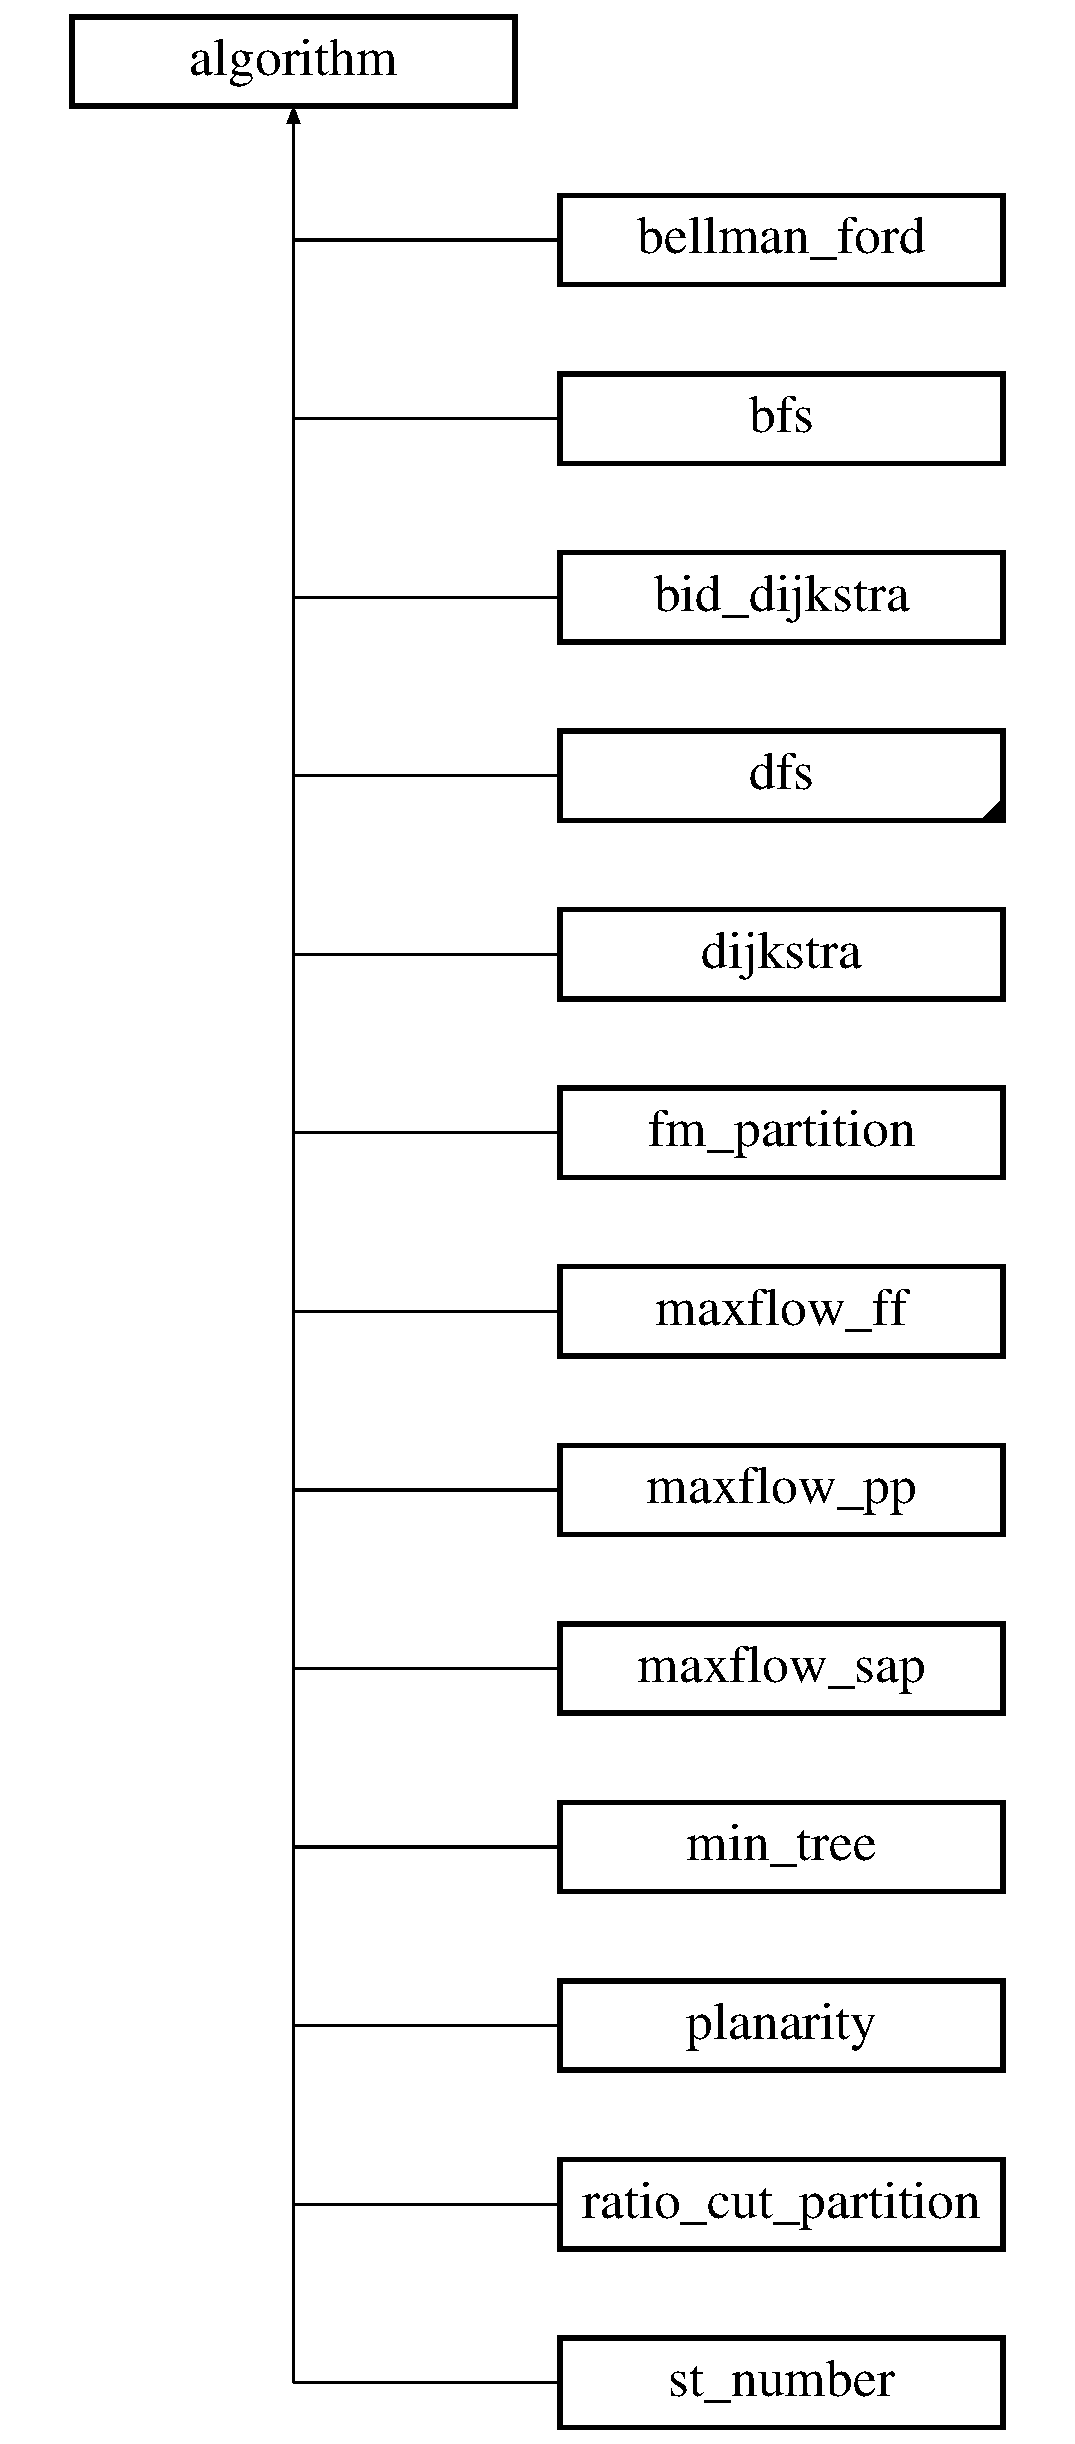
\includegraphics[height=12.000000cm]{classalgorithm}
\end{center}
\end{figure}
\subsection*{Public Types}
\begin{DoxyCompactItemize}
\item 
enum \{ \mbox{\hyperlink{classalgorithm_af1a0078e153aa99c24f9bdf0d97f6710aae4c1cd7fe8d8cf4b143241a6e7c31cf}{K\+G\+L\+\_\+\+OK}} = 1, 
\mbox{\hyperlink{classalgorithm_af1a0078e153aa99c24f9bdf0d97f6710ae67bf27b2ef31f73e545a7f9f4a69556}{K\+G\+L\+\_\+\+E\+R\+R\+OR}} = 0
 \}
\begin{DoxyCompactList}\small\item\em Return values for \mbox{\hyperlink{classalgorithm_a76361fb03ad1cf643affc51821e43bed}{algorithm\+::check}} and \mbox{\hyperlink{classalgorithm_a734b189509a8d6b56b65f8ff772d43ca}{algorithm\+::run}}. \end{DoxyCompactList}\end{DoxyCompactItemize}
\subsection*{Public Member Functions}
\begin{DoxyCompactItemize}
\item 
\mbox{\Hypertarget{classalgorithm_ab79e1ddec2f2afdf4b36b10724db8b15}\label{classalgorithm_ab79e1ddec2f2afdf4b36b10724db8b15}} 
\mbox{\hyperlink{classalgorithm_ab79e1ddec2f2afdf4b36b10724db8b15}{algorithm}} ()
\begin{DoxyCompactList}\small\item\em Creates an algorithm object. \end{DoxyCompactList}\item 
\mbox{\Hypertarget{classalgorithm_adca9b1e7fa3afd914519a9dbb44e9fd5}\label{classalgorithm_adca9b1e7fa3afd914519a9dbb44e9fd5}} 
virtual \mbox{\hyperlink{classalgorithm_adca9b1e7fa3afd914519a9dbb44e9fd5}{$\sim$algorithm}} ()
\begin{DoxyCompactList}\small\item\em Destroys the algorithm object. \end{DoxyCompactList}\item 
virtual int \mbox{\hyperlink{classalgorithm_a734b189509a8d6b56b65f8ff772d43ca}{run}} (\mbox{\hyperlink{classgraph}{graph}} \&g)=0
\begin{DoxyCompactList}\small\item\em Applies algorithm to graph g. \end{DoxyCompactList}\item 
virtual int \mbox{\hyperlink{classalgorithm_a76361fb03ad1cf643affc51821e43bed}{check}} (\mbox{\hyperlink{classgraph}{graph}} \&g)=0
\begin{DoxyCompactList}\small\item\em Checks whether all preconditions are satisfied. \end{DoxyCompactList}\item 
virtual void \mbox{\hyperlink{classalgorithm_a21aba63d066ae7897de6ca7d8425c408}{reset}} ()=0
\begin{DoxyCompactList}\small\item\em Resets algorithm. \end{DoxyCompactList}\end{DoxyCompactItemize}


\subsection{Detailed Description}
Abstract baseclass for all algoritm-\/classes. 

\begin{DoxyParagraph}{Date}
2019/05/07 15\+:58\+:54 
\end{DoxyParagraph}
\begin{DoxyParagraph}{Revision}
1.\+14 
\end{DoxyParagraph}


\subsection{Member Enumeration Documentation}
\mbox{\Hypertarget{classalgorithm_af1a0078e153aa99c24f9bdf0d97f6710}\label{classalgorithm_af1a0078e153aa99c24f9bdf0d97f6710}} 
\subsubsection{\texorpdfstring{anonymous enum}{anonymous enum}}
{\footnotesize\ttfamily anonymous enum}



Return values for \mbox{\hyperlink{classalgorithm_a76361fb03ad1cf643affc51821e43bed}{algorithm\+::check}} and \mbox{\hyperlink{classalgorithm_a734b189509a8d6b56b65f8ff772d43ca}{algorithm\+::run}}. 

\begin{DoxyEnumFields}{Enumerator}
\raisebox{\heightof{T}}[0pt][0pt]{\index{K\+G\+L\+\_\+\+OK@{K\+G\+L\+\_\+\+OK}!algorithm@{algorithm}}\index{algorithm@{algorithm}!K\+G\+L\+\_\+\+OK@{K\+G\+L\+\_\+\+OK}}}\mbox{\Hypertarget{classalgorithm_af1a0078e153aa99c24f9bdf0d97f6710aae4c1cd7fe8d8cf4b143241a6e7c31cf}\label{classalgorithm_af1a0078e153aa99c24f9bdf0d97f6710aae4c1cd7fe8d8cf4b143241a6e7c31cf}} 
K\+G\+L\+\_\+\+OK&Used as (positive) return value of \mbox{\hyperlink{classalgorithm_a76361fb03ad1cf643affc51821e43bed}{algorithm\+::check}} and \mbox{\hyperlink{classalgorithm_a734b189509a8d6b56b65f8ff772d43ca}{algorithm\+::run}}. \\
\hline

\raisebox{\heightof{T}}[0pt][0pt]{\index{K\+G\+L\+\_\+\+E\+R\+R\+OR@{K\+G\+L\+\_\+\+E\+R\+R\+OR}!algorithm@{algorithm}}\index{algorithm@{algorithm}!K\+G\+L\+\_\+\+E\+R\+R\+OR@{K\+G\+L\+\_\+\+E\+R\+R\+OR}}}\mbox{\Hypertarget{classalgorithm_af1a0078e153aa99c24f9bdf0d97f6710ae67bf27b2ef31f73e545a7f9f4a69556}\label{classalgorithm_af1a0078e153aa99c24f9bdf0d97f6710ae67bf27b2ef31f73e545a7f9f4a69556}} 
K\+G\+L\+\_\+\+E\+R\+R\+OR&Used as (negative) return value of \mbox{\hyperlink{classalgorithm_a76361fb03ad1cf643affc51821e43bed}{algorithm\+::check}} and \mbox{\hyperlink{classalgorithm_a734b189509a8d6b56b65f8ff772d43ca}{algorithm\+::run}}. \\
\hline

\end{DoxyEnumFields}


\subsection{Member Function Documentation}
\mbox{\Hypertarget{classalgorithm_a76361fb03ad1cf643affc51821e43bed}\label{classalgorithm_a76361fb03ad1cf643affc51821e43bed}} 
\index{algorithm@{algorithm}!check@{check}}
\index{check@{check}!algorithm@{algorithm}}
\subsubsection{\texorpdfstring{check()}{check()}}
{\footnotesize\ttfamily virtual int algorithm\+::check (\begin{DoxyParamCaption}\item[{\mbox{\hyperlink{classgraph}{graph}} \&}]{g }\end{DoxyParamCaption})\hspace{0.3cm}{\ttfamily [pure virtual]}}



Checks whether all preconditions are satisfied. 

{\itshape Please} {\itshape note\+:} It is definitly required (and \mbox{\hyperlink{classalgorithm_a734b189509a8d6b56b65f8ff772d43ca}{run}} relies on it), that this method was called in advance.


\begin{DoxyParams}{Parameters}
{\em g} & graph \\
\hline
\end{DoxyParams}

\begin{DoxyRetVals}{Return values}
{\em \mbox{\hyperlink{classalgorithm_af1a0078e153aa99c24f9bdf0d97f6710aae4c1cd7fe8d8cf4b143241a6e7c31cf}{algorithm\+::\+K\+G\+L\+\_\+\+OK}}} & if algorithm can be applied \\
\hline
{\em \mbox{\hyperlink{classalgorithm_af1a0078e153aa99c24f9bdf0d97f6710ae67bf27b2ef31f73e545a7f9f4a69556}{algorithm\+::\+K\+G\+L\+\_\+\+E\+R\+R\+OR}}} & otherwise. \\
\hline
\end{DoxyRetVals}


Implemented in \mbox{\hyperlink{classst__number_a2aad4550b821c52d6998bff35fd8648f}{st\+\_\+number}}, \mbox{\hyperlink{classratio__cut__partition_a469c613c69db19cb63e492075346fea2}{ratio\+\_\+cut\+\_\+partition}}, \mbox{\hyperlink{classfm__partition_af72a9fcc300ab0f202168c819b089e5d}{fm\+\_\+partition}}, \mbox{\hyperlink{classdijkstra_a51ff4657e0ddb1ca5231a21e6dea1808}{dijkstra}}, \mbox{\hyperlink{classbid__dijkstra_a504aa04d114f27f2f886ee3b025ad95b}{bid\+\_\+dijkstra}}, \mbox{\hyperlink{classdfs_a1af70060897529e67910f589b047e576}{dfs}}, \mbox{\hyperlink{classbfs_a6dd7e852f7768814aafba8962befca56}{bfs}}, \mbox{\hyperlink{classtopsort_a777a9a68c4081d22e7b698ed3c515343}{topsort}}, \mbox{\hyperlink{classmaxflow__sap_aa2974bf25fb597677848fdb23c12d338}{maxflow\+\_\+sap}}, \mbox{\hyperlink{classmaxflow__ff_a4d0deee7d70bac4c9dad942341d87e37}{maxflow\+\_\+ff}}, \mbox{\hyperlink{classmaxflow__pp_a7ea24bd88999718e5e4e28ac028131cd}{maxflow\+\_\+pp}}, \mbox{\hyperlink{classplanarity_ae06c471d957a116aad14e338c341f8b1}{planarity}}, \mbox{\hyperlink{classbiconnectivity_a65e0e821f5e9ce8d210648d462fd2cfa}{biconnectivity}}, \mbox{\hyperlink{classbellman__ford_a9da2fb7d20ef1f726ee935474302d80b}{bellman\+\_\+ford}}, \mbox{\hyperlink{classmin__tree_ad87b1bfbc687ad943c07538fa0c3d270}{min\+\_\+tree}}, and \mbox{\hyperlink{classcomponents_aeeda901d02c65d6c31c8b6148540d7c1}{components}}.

\mbox{\Hypertarget{classalgorithm_a21aba63d066ae7897de6ca7d8425c408}\label{classalgorithm_a21aba63d066ae7897de6ca7d8425c408}} 
\index{algorithm@{algorithm}!reset@{reset}}
\index{reset@{reset}!algorithm@{algorithm}}
\subsubsection{\texorpdfstring{reset()}{reset()}}
{\footnotesize\ttfamily virtual void algorithm\+::reset (\begin{DoxyParamCaption}{ }\end{DoxyParamCaption})\hspace{0.3cm}{\ttfamily [pure virtual]}}



Resets algorithm. 

Prepares the algorithm to be applied to another graph. {\itshape Please} {\itshape note\+:} The options an algorithm may support do {\itshape not} get reset by this. It is just to reset internally used datastructures. 

Implemented in \mbox{\hyperlink{classst__number_ae6f86706b8ae3495d3794b8c684fff0f}{st\+\_\+number}}, \mbox{\hyperlink{classratio__cut__partition_ad017eaf98f9ae4ca9dbe6b3eda9fc94d}{ratio\+\_\+cut\+\_\+partition}}, \mbox{\hyperlink{classfm__partition_a6db2eeb6ae968dbab78302f0448c0ced}{fm\+\_\+partition}}, \mbox{\hyperlink{classdijkstra_a444c288b3a49ec1c2973459dad55ffb3}{dijkstra}}, \mbox{\hyperlink{classbid__dijkstra_a6df2769941bc73fc5626b084745a2258}{bid\+\_\+dijkstra}}, \mbox{\hyperlink{classmaxflow__sap_a14574d2f9ce31a3cdeb0888e57fc0616}{maxflow\+\_\+sap}}, \mbox{\hyperlink{classmaxflow__ff_a893e5136d4f7f1d4b67ef5b67306d17b}{maxflow\+\_\+ff}}, \mbox{\hyperlink{classmaxflow__pp_a2179764baf624f1414211f3a7181b1a0}{maxflow\+\_\+pp}}, \mbox{\hyperlink{classdfs_affaffda8be8418d6dbf396c5b1d6b81a}{dfs}}, \mbox{\hyperlink{classbfs_a6398bc230f9723cd5fdd32cd603647cc}{bfs}}, \mbox{\hyperlink{classplanarity_aca500e3d46a99c6231aff86afa2a71b1}{planarity}}, \mbox{\hyperlink{classtopsort_af93d2f617ceae83ee2a4f9106fbc32c3}{topsort}}, \mbox{\hyperlink{classbellman__ford_a7d28afa62ce8068c4d0f2d1f96136fd6}{bellman\+\_\+ford}}, \mbox{\hyperlink{classbiconnectivity_a4393dd1e626887472f6967722349abc6}{biconnectivity}}, \mbox{\hyperlink{classmin__tree_a0edbe612424dc5f4de4701b8fd0df931}{min\+\_\+tree}}, and \mbox{\hyperlink{classcomponents_a07b6bab5962524ae26ccb478b35cd76c}{components}}.

\mbox{\Hypertarget{classalgorithm_a734b189509a8d6b56b65f8ff772d43ca}\label{classalgorithm_a734b189509a8d6b56b65f8ff772d43ca}} 
\index{algorithm@{algorithm}!run@{run}}
\index{run@{run}!algorithm@{algorithm}}
\subsubsection{\texorpdfstring{run()}{run()}}
{\footnotesize\ttfamily virtual int algorithm\+::run (\begin{DoxyParamCaption}\item[{\mbox{\hyperlink{classgraph}{graph}} \&}]{g }\end{DoxyParamCaption})\hspace{0.3cm}{\ttfamily [pure virtual]}}



Applies algorithm to graph g. 


\begin{DoxyParams}{Parameters}
{\em g} & graph \\
\hline
\end{DoxyParams}

\begin{DoxyRetVals}{Return values}
{\em \mbox{\hyperlink{classalgorithm_af1a0078e153aa99c24f9bdf0d97f6710aae4c1cd7fe8d8cf4b143241a6e7c31cf}{algorithm\+::\+K\+G\+L\+\_\+\+OK}}} & on success \\
\hline
{\em \mbox{\hyperlink{classalgorithm_af1a0078e153aa99c24f9bdf0d97f6710ae67bf27b2ef31f73e545a7f9f4a69556}{algorithm\+::\+K\+G\+L\+\_\+\+E\+R\+R\+OR}}} & otherwise \\
\hline
\end{DoxyRetVals}


Implemented in \mbox{\hyperlink{classst__number_af902a0c05d07d47b587e8f7a6b7beaa1}{st\+\_\+number}}, \mbox{\hyperlink{classratio__cut__partition_a4ab180ca4cf57c811e3478c3de4c4dc3}{ratio\+\_\+cut\+\_\+partition}}, \mbox{\hyperlink{classfm__partition_a015b171fcaa01973ebe6c6a46a727097}{fm\+\_\+partition}}, \mbox{\hyperlink{classdijkstra_a7b30f3d8ad42baae27989bc14befe0d0}{dijkstra}}, \mbox{\hyperlink{classbid__dijkstra_a1d2f36d3977ef90285442a269a03b919}{bid\+\_\+dijkstra}}, \mbox{\hyperlink{classdfs_af0863b8974d5fd58cd0375c78ed8163b}{dfs}}, \mbox{\hyperlink{classbfs_a06ae16bd0f3bb2f8eb6b3e36659ba82e}{bfs}}, \mbox{\hyperlink{classmaxflow__sap_ab4305a2bb370ad9c43cc68d339b2dda0}{maxflow\+\_\+sap}}, \mbox{\hyperlink{classplanarity_a93232e765c08dd2a4c00d192bb48b5fc}{planarity}}, \mbox{\hyperlink{classmaxflow__ff_a0a4391b9093d6966b47c023a555099e2}{maxflow\+\_\+ff}}, \mbox{\hyperlink{classmaxflow__pp_a07c7cb1ae5db23d87cf49ce7769b2814}{maxflow\+\_\+pp}}, \mbox{\hyperlink{classbellman__ford_a226308389f3c36dfc02768c09f777a3b}{bellman\+\_\+ford}}, and \mbox{\hyperlink{classmin__tree_ac025e8dad0db7a6a1e0e7b476b547802}{min\+\_\+tree}}.



The documentation for this class was generated from the following file\+:\begin{DoxyCompactItemize}
\item 
include/\+K\+G\+L/algorithm.\+h\end{DoxyCompactItemize}

\hypertarget{classbellman__ford}{}\section{bellman\+\_\+ford Class Reference}
\label{classbellman__ford}\index{bellman\+\_\+ford@{bellman\+\_\+ford}}


Bellman Ford algorithm.  




{\ttfamily \#include $<$bellman\+\_\+ford.\+h$>$}

Inheritance diagram for bellman\+\_\+ford\+:\begin{figure}[H]
\begin{center}
\leavevmode
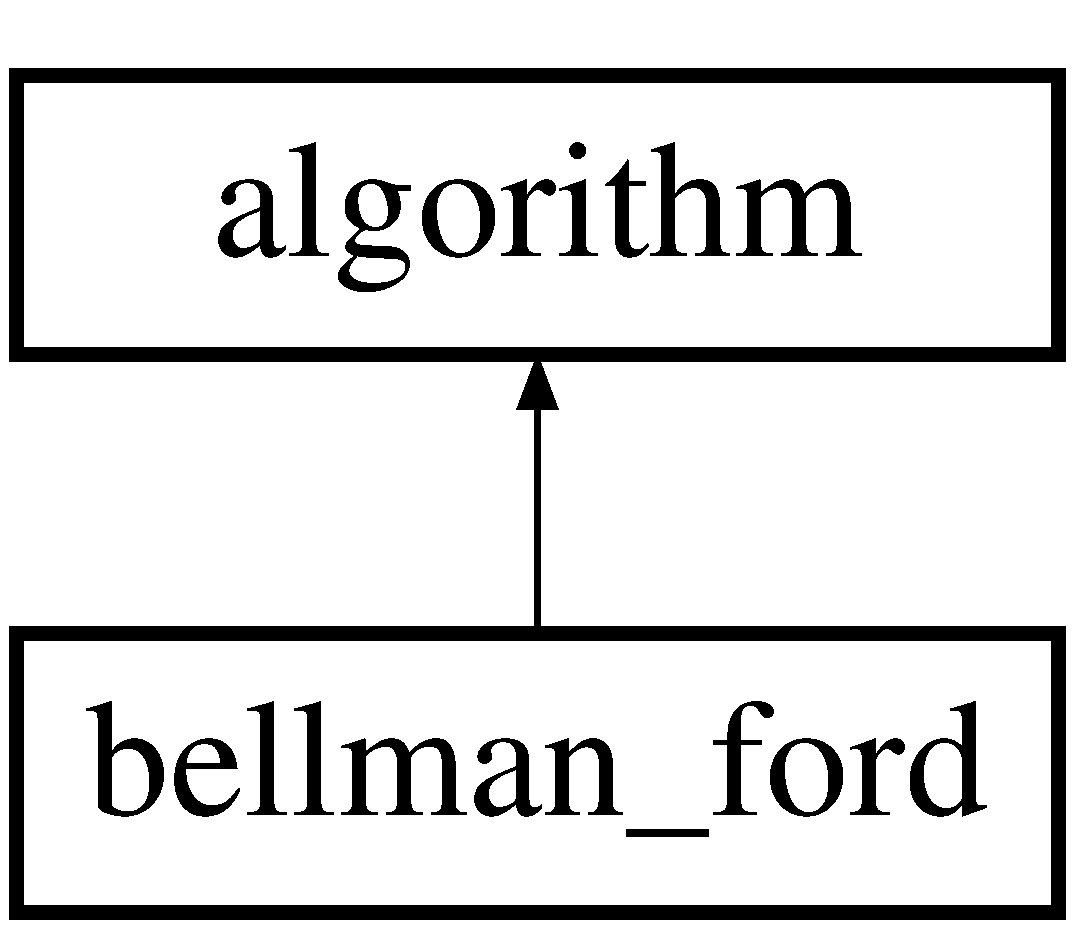
\includegraphics[height=2.000000cm]{classbellman__ford}
\end{center}
\end{figure}
\subsection*{Public Member Functions}
\begin{DoxyCompactItemize}
\item 
\mbox{\Hypertarget{classbellman__ford_ae732e7ea1c63e3ed64779b31a3a9a208}\label{classbellman__ford_ae732e7ea1c63e3ed64779b31a3a9a208}} 
\mbox{\hyperlink{classbellman__ford_ae732e7ea1c63e3ed64779b31a3a9a208}{bellman\+\_\+ford}} ()
\begin{DoxyCompactList}\small\item\em Constructor. \end{DoxyCompactList}\item 
\mbox{\Hypertarget{classbellman__ford_a8461c6b8d7663b05a97b6d270347a49c}\label{classbellman__ford_a8461c6b8d7663b05a97b6d270347a49c}} 
virtual \mbox{\hyperlink{classbellman__ford_a8461c6b8d7663b05a97b6d270347a49c}{$\sim$bellman\+\_\+ford}} ()
\begin{DoxyCompactList}\small\item\em Destructor. \end{DoxyCompactList}\item 
int \mbox{\hyperlink{classbellman__ford_a9da2fb7d20ef1f726ee935474302d80b}{check}} (\mbox{\hyperlink{classgraph}{graph}} \&G)
\begin{DoxyCompactList}\small\item\em Checks whether the preconditions for Bellman Ford are satisfied. \end{DoxyCompactList}\item 
int \mbox{\hyperlink{classbellman__ford_a226308389f3c36dfc02768c09f777a3b}{run}} (\mbox{\hyperlink{classgraph}{graph}} \&G)
\begin{DoxyCompactList}\small\item\em Applies algorithm to graph g. \end{DoxyCompactList}\item 
void \mbox{\hyperlink{classbellman__ford_a7d28afa62ce8068c4d0f2d1f96136fd6}{reset}} ()
\begin{DoxyCompactList}\small\item\em Resets the algorithm. \end{DoxyCompactList}\item 
void \mbox{\hyperlink{classbellman__ford_a98cad540fd2d211c1ba44bb6fa8416f3}{source}} (const \mbox{\hyperlink{classnode}{node}} \&n)
\begin{DoxyCompactList}\small\item\em Sets source. \end{DoxyCompactList}\item 
\mbox{\hyperlink{classnode}{node}} \mbox{\hyperlink{classbellman__ford_a86e3fe7fe71d7569cc73e9e531d58539}{source}} () const
\begin{DoxyCompactList}\small\item\em Returns source. \end{DoxyCompactList}\item 
void \mbox{\hyperlink{classbellman__ford_a9e276cc9f30c2e608d320db4a08b2a74}{weights}} (const \mbox{\hyperlink{classedge__map}{edge\+\_\+map}}$<$ double $>$ \&weight)
\begin{DoxyCompactList}\small\item\em Sets weights of the edges. \end{DoxyCompactList}\item 
void \mbox{\hyperlink{classbellman__ford_aac87169a3cf4f95477ce215a0cb7a12b}{store\+\_\+preds}} (bool set)
\begin{DoxyCompactList}\small\item\em Enables or disables the storing of predecessors. \end{DoxyCompactList}\item 
bool \mbox{\hyperlink{classbellman__ford_a2ded0950bfaca6c3ee65a3617c1ccaa8}{store\+\_\+preds}} () const
\begin{DoxyCompactList}\small\item\em Returns whether the storing of predecessors is enabled. \end{DoxyCompactList}\item 
bool \mbox{\hyperlink{classbellman__ford_a93f7c34ec9662690230ca7a9c31933cd}{reached}} (const \mbox{\hyperlink{classnode}{node}} \&n) const
\begin{DoxyCompactList}\small\item\em Returns whether is reachable from source. \end{DoxyCompactList}\item 
double \mbox{\hyperlink{classbellman__ford_a881e5b021e69aced997185208438f910}{distance}} (const \mbox{\hyperlink{classnode}{node}} \&n) const
\begin{DoxyCompactList}\small\item\em Returns the distance from source to {\itshape n}. \end{DoxyCompactList}\item 
\mbox{\hyperlink{classedge}{edge}} \mbox{\hyperlink{classbellman__ford_a39f93b0b1e427cf26059fa6141c6f61c}{predecessor\+\_\+edge}} (const \mbox{\hyperlink{classnode}{node}} \&n) const
\begin{DoxyCompactList}\small\item\em edge to predecessor of node {\itshape n} on the shortest path from source \end{DoxyCompactList}\item 
\mbox{\hyperlink{classnode}{node}} \mbox{\hyperlink{classbellman__ford_a403e286ec8cbe3c30a7a729c5041155e}{predecessor\+\_\+node}} (const \mbox{\hyperlink{classnode}{node}} \&n) const
\begin{DoxyCompactList}\small\item\em predecessor of node {\itshape n} on the shortest path from source \end{DoxyCompactList}\item 
\mbox{\Hypertarget{classbellman__ford_af9cd8be38bb1504089997581d9aa4f64}\label{classbellman__ford_af9cd8be38bb1504089997581d9aa4f64}} 
bool \mbox{\hyperlink{classbellman__ford_af9cd8be38bb1504089997581d9aa4f64}{negative\+\_\+cycle}} () const
\begin{DoxyCompactList}\small\item\em Returns whether there is a cycle with negative weight. \end{DoxyCompactList}\end{DoxyCompactItemize}
\subsection*{Additional Inherited Members}


\subsection{Detailed Description}
Bellman Ford algorithm. 

\begin{DoxyParagraph}{Date}
2019/05/07 15\+:58\+:54 
\end{DoxyParagraph}
\begin{DoxyParagraph}{Revision}
1.\+5 
\end{DoxyParagraph}


Implementation of the single source shortest path due to Bellman and Ford. Unlike Dijkstra\textquotesingle{}s S\+S\+SP algorithm this one allows negative edge weights, as long as there are no cycles with negative weight. If there are negative cycles this implementation finds them. 

\subsection{Member Function Documentation}
\mbox{\Hypertarget{classbellman__ford_a9da2fb7d20ef1f726ee935474302d80b}\label{classbellman__ford_a9da2fb7d20ef1f726ee935474302d80b}} 
\index{bellman\+\_\+ford@{bellman\+\_\+ford}!check@{check}}
\index{check@{check}!bellman\+\_\+ford@{bellman\+\_\+ford}}
\subsubsection{\texorpdfstring{check()}{check()}}
{\footnotesize\ttfamily int bellman\+\_\+ford\+::check (\begin{DoxyParamCaption}\item[{\mbox{\hyperlink{classgraph}{graph}} \&}]{G }\end{DoxyParamCaption})\hspace{0.3cm}{\ttfamily [virtual]}}



Checks whether the preconditions for Bellman Ford are satisfied. 

The Precondition are that the weights of the edges have been set and that the graph has at least one node.


\begin{DoxyParams}{Parameters}
{\em G} & graph. \\
\hline
\end{DoxyParams}

\begin{DoxyRetVals}{Return values}
{\em \mbox{\hyperlink{classalgorithm_af1a0078e153aa99c24f9bdf0d97f6710aae4c1cd7fe8d8cf4b143241a6e7c31cf}{algorithm\+::\+K\+G\+L\+\_\+\+OK}}} & if algorithm can be applied \\
\hline
{\em \mbox{\hyperlink{classalgorithm_af1a0078e153aa99c24f9bdf0d97f6710ae67bf27b2ef31f73e545a7f9f4a69556}{algorithm\+::\+K\+G\+L\+\_\+\+E\+R\+R\+OR}}} & otherwise. \\
\hline
\end{DoxyRetVals}


Implements \mbox{\hyperlink{classalgorithm_a76361fb03ad1cf643affc51821e43bed}{algorithm}}.

\mbox{\Hypertarget{classbellman__ford_a881e5b021e69aced997185208438f910}\label{classbellman__ford_a881e5b021e69aced997185208438f910}} 
\index{bellman\+\_\+ford@{bellman\+\_\+ford}!distance@{distance}}
\index{distance@{distance}!bellman\+\_\+ford@{bellman\+\_\+ford}}
\subsubsection{\texorpdfstring{distance()}{distance()}}
{\footnotesize\ttfamily double bellman\+\_\+ford\+::distance (\begin{DoxyParamCaption}\item[{const \mbox{\hyperlink{classnode}{node}} \&}]{n }\end{DoxyParamCaption}) const\hspace{0.3cm}{\ttfamily [inline]}}



Returns the distance from source to {\itshape n}. 


\begin{DoxyParams}{Parameters}
{\em n} & node \\
\hline
\end{DoxyParams}
\mbox{\Hypertarget{classbellman__ford_a39f93b0b1e427cf26059fa6141c6f61c}\label{classbellman__ford_a39f93b0b1e427cf26059fa6141c6f61c}} 
\index{bellman\+\_\+ford@{bellman\+\_\+ford}!predecessor\+\_\+edge@{predecessor\+\_\+edge}}
\index{predecessor\+\_\+edge@{predecessor\+\_\+edge}!bellman\+\_\+ford@{bellman\+\_\+ford}}
\subsubsection{\texorpdfstring{predecessor\+\_\+edge()}{predecessor\_edge()}}
{\footnotesize\ttfamily \mbox{\hyperlink{classedge}{edge}} bellman\+\_\+ford\+::predecessor\+\_\+edge (\begin{DoxyParamCaption}\item[{const \mbox{\hyperlink{classnode}{node}} \&}]{n }\end{DoxyParamCaption}) const\hspace{0.3cm}{\ttfamily [inline]}}



edge to predecessor of node {\itshape n} on the shortest path from source 

If {\itshape n} is a root or wasn\textquotesingle{}t reached the return value is the invalid edge \mbox{\hyperlink{classedge_a41859d2473a15e24255d7bc0de1f49b4}{edge\+::edge()}}.

{\itshape Please} {\itshape note} that this requires that this option was enabled during last run.


\begin{DoxyParams}{Parameters}
{\em n} & node. \\
\hline
\end{DoxyParams}
\begin{DoxyReturn}{Returns}
predecessor of {\itshape n}. 
\end{DoxyReturn}
\begin{DoxySeeAlso}{See also}
\mbox{\hyperlink{classbellman__ford_aac87169a3cf4f95477ce215a0cb7a12b}{bellman\+\_\+ford\+::store\+\_\+preds}} 
\end{DoxySeeAlso}
\mbox{\Hypertarget{classbellman__ford_a403e286ec8cbe3c30a7a729c5041155e}\label{classbellman__ford_a403e286ec8cbe3c30a7a729c5041155e}} 
\index{bellman\+\_\+ford@{bellman\+\_\+ford}!predecessor\+\_\+node@{predecessor\+\_\+node}}
\index{predecessor\+\_\+node@{predecessor\+\_\+node}!bellman\+\_\+ford@{bellman\+\_\+ford}}
\subsubsection{\texorpdfstring{predecessor\+\_\+node()}{predecessor\_node()}}
{\footnotesize\ttfamily \mbox{\hyperlink{classnode}{node}} bellman\+\_\+ford\+::predecessor\+\_\+node (\begin{DoxyParamCaption}\item[{const \mbox{\hyperlink{classnode}{node}} \&}]{n }\end{DoxyParamCaption}) const\hspace{0.3cm}{\ttfamily [inline]}}



predecessor of node {\itshape n} on the shortest path from source 

If {\itshape n} is a root or wasn\textquotesingle{}t reached the return value is the invalid node \mbox{\hyperlink{classnode_ad603259398d5667e3b97a6322a2bcc20}{node\+::node()}}.

{\itshape Please} {\itshape note} that this requires that this option was enabled during last run.


\begin{DoxyParams}{Parameters}
{\em n} & node. \\
\hline
\end{DoxyParams}
\begin{DoxyReturn}{Returns}
predecessor of {\itshape n}. 
\end{DoxyReturn}
\begin{DoxySeeAlso}{See also}
\mbox{\hyperlink{classbellman__ford_aac87169a3cf4f95477ce215a0cb7a12b}{bellman\+\_\+ford\+::store\+\_\+preds}} 
\end{DoxySeeAlso}
\mbox{\Hypertarget{classbellman__ford_a93f7c34ec9662690230ca7a9c31933cd}\label{classbellman__ford_a93f7c34ec9662690230ca7a9c31933cd}} 
\index{bellman\+\_\+ford@{bellman\+\_\+ford}!reached@{reached}}
\index{reached@{reached}!bellman\+\_\+ford@{bellman\+\_\+ford}}
\subsubsection{\texorpdfstring{reached()}{reached()}}
{\footnotesize\ttfamily bool bellman\+\_\+ford\+::reached (\begin{DoxyParamCaption}\item[{const \mbox{\hyperlink{classnode}{node}} \&}]{n }\end{DoxyParamCaption}) const\hspace{0.3cm}{\ttfamily [inline]}}



Returns whether is reachable from source. 


\begin{DoxyParams}{Parameters}
{\em n} & node \\
\hline
\end{DoxyParams}
\mbox{\Hypertarget{classbellman__ford_a7d28afa62ce8068c4d0f2d1f96136fd6}\label{classbellman__ford_a7d28afa62ce8068c4d0f2d1f96136fd6}} 
\index{bellman\+\_\+ford@{bellman\+\_\+ford}!reset@{reset}}
\index{reset@{reset}!bellman\+\_\+ford@{bellman\+\_\+ford}}
\subsubsection{\texorpdfstring{reset()}{reset()}}
{\footnotesize\ttfamily void bellman\+\_\+ford\+::reset (\begin{DoxyParamCaption}{ }\end{DoxyParamCaption})\hspace{0.3cm}{\ttfamily [virtual]}}



Resets the algorithm. 

The weights are not reset. You can apply this algorithms twice without setting the weights for the second call. 

Implements \mbox{\hyperlink{classalgorithm_a21aba63d066ae7897de6ca7d8425c408}{algorithm}}.

\mbox{\Hypertarget{classbellman__ford_a226308389f3c36dfc02768c09f777a3b}\label{classbellman__ford_a226308389f3c36dfc02768c09f777a3b}} 
\index{bellman\+\_\+ford@{bellman\+\_\+ford}!run@{run}}
\index{run@{run}!bellman\+\_\+ford@{bellman\+\_\+ford}}
\subsubsection{\texorpdfstring{run()}{run()}}
{\footnotesize\ttfamily int bellman\+\_\+ford\+::run (\begin{DoxyParamCaption}\item[{\mbox{\hyperlink{classgraph}{graph}} \&}]{g }\end{DoxyParamCaption})\hspace{0.3cm}{\ttfamily [virtual]}}



Applies algorithm to graph g. 


\begin{DoxyParams}{Parameters}
{\em g} & graph \\
\hline
\end{DoxyParams}

\begin{DoxyRetVals}{Return values}
{\em \mbox{\hyperlink{classalgorithm_af1a0078e153aa99c24f9bdf0d97f6710aae4c1cd7fe8d8cf4b143241a6e7c31cf}{algorithm\+::\+K\+G\+L\+\_\+\+OK}}} & on success \\
\hline
{\em \mbox{\hyperlink{classalgorithm_af1a0078e153aa99c24f9bdf0d97f6710ae67bf27b2ef31f73e545a7f9f4a69556}{algorithm\+::\+K\+G\+L\+\_\+\+E\+R\+R\+OR}}} & otherwise \\
\hline
\end{DoxyRetVals}


Implements \mbox{\hyperlink{classalgorithm_a734b189509a8d6b56b65f8ff772d43ca}{algorithm}}.

\mbox{\Hypertarget{classbellman__ford_a98cad540fd2d211c1ba44bb6fa8416f3}\label{classbellman__ford_a98cad540fd2d211c1ba44bb6fa8416f3}} 
\index{bellman\+\_\+ford@{bellman\+\_\+ford}!source@{source}}
\index{source@{source}!bellman\+\_\+ford@{bellman\+\_\+ford}}
\subsubsection{\texorpdfstring{source()}{source()}\hspace{0.1cm}{\footnotesize\ttfamily [1/2]}}
{\footnotesize\ttfamily void bellman\+\_\+ford\+::source (\begin{DoxyParamCaption}\item[{const \mbox{\hyperlink{classnode}{node}} \&}]{n }\end{DoxyParamCaption})\hspace{0.3cm}{\ttfamily [inline]}}



Sets source. 

The default source is the invalid node (\mbox{\hyperlink{classnode_ad603259398d5667e3b97a6322a2bcc20}{node\+::node()}}), in this case an arbitrary node is chosen and stored when this algorithm is run.


\begin{DoxyParams}{Parameters}
{\em n} & source. \\
\hline
\end{DoxyParams}
\mbox{\Hypertarget{classbellman__ford_a86e3fe7fe71d7569cc73e9e531d58539}\label{classbellman__ford_a86e3fe7fe71d7569cc73e9e531d58539}} 
\index{bellman\+\_\+ford@{bellman\+\_\+ford}!source@{source}}
\index{source@{source}!bellman\+\_\+ford@{bellman\+\_\+ford}}
\subsubsection{\texorpdfstring{source()}{source()}\hspace{0.1cm}{\footnotesize\ttfamily [2/2]}}
{\footnotesize\ttfamily \mbox{\hyperlink{classnode}{node}} bellman\+\_\+ford\+::source (\begin{DoxyParamCaption}{ }\end{DoxyParamCaption}) const\hspace{0.3cm}{\ttfamily [inline]}}



Returns source. 

\begin{DoxyReturn}{Returns}
source. 
\end{DoxyReturn}
\mbox{\Hypertarget{classbellman__ford_aac87169a3cf4f95477ce215a0cb7a12b}\label{classbellman__ford_aac87169a3cf4f95477ce215a0cb7a12b}} 
\index{bellman\+\_\+ford@{bellman\+\_\+ford}!store\+\_\+preds@{store\+\_\+preds}}
\index{store\+\_\+preds@{store\+\_\+preds}!bellman\+\_\+ford@{bellman\+\_\+ford}}
\subsubsection{\texorpdfstring{store\+\_\+preds()}{store\_preds()}\hspace{0.1cm}{\footnotesize\ttfamily [1/2]}}
{\footnotesize\ttfamily void bellman\+\_\+ford\+::store\+\_\+preds (\begin{DoxyParamCaption}\item[{bool}]{set }\end{DoxyParamCaption})}



Enables or disables the storing of predecessors. 

If enabled for every node the predecessor on the shortest path from will be stored.


\begin{DoxyParams}{Parameters}
{\em set} & if true predecessors will be stored. \\
\hline
\end{DoxyParams}
\begin{DoxySeeAlso}{See also}
\mbox{\hyperlink{classbellman__ford_a403e286ec8cbe3c30a7a729c5041155e}{bellman\+\_\+ford\+::predecessor\+\_\+node}}, \mbox{\hyperlink{classbellman__ford_a39f93b0b1e427cf26059fa6141c6f61c}{bellman\+\_\+ford\+::predecessor\+\_\+edge}} 
\end{DoxySeeAlso}
\mbox{\Hypertarget{classbellman__ford_a2ded0950bfaca6c3ee65a3617c1ccaa8}\label{classbellman__ford_a2ded0950bfaca6c3ee65a3617c1ccaa8}} 
\index{bellman\+\_\+ford@{bellman\+\_\+ford}!store\+\_\+preds@{store\+\_\+preds}}
\index{store\+\_\+preds@{store\+\_\+preds}!bellman\+\_\+ford@{bellman\+\_\+ford}}
\subsubsection{\texorpdfstring{store\+\_\+preds()}{store\_preds()}\hspace{0.1cm}{\footnotesize\ttfamily [2/2]}}
{\footnotesize\ttfamily bool bellman\+\_\+ford\+::store\+\_\+preds (\begin{DoxyParamCaption}{ }\end{DoxyParamCaption}) const\hspace{0.3cm}{\ttfamily [inline]}}



Returns whether the storing of predecessors is enabled. 


\begin{DoxyRetVals}{Return values}
{\em true} & iff the storing of predecessors is enabled. ~\newline
 \\
\hline
\end{DoxyRetVals}
\begin{DoxySeeAlso}{See also}
\mbox{\hyperlink{classbellman__ford_a403e286ec8cbe3c30a7a729c5041155e}{bellman\+\_\+ford\+::predecessor\+\_\+node}}, \mbox{\hyperlink{classbellman__ford_a39f93b0b1e427cf26059fa6141c6f61c}{bellman\+\_\+ford\+::predecessor\+\_\+edge}} 
\end{DoxySeeAlso}
\mbox{\Hypertarget{classbellman__ford_a9e276cc9f30c2e608d320db4a08b2a74}\label{classbellman__ford_a9e276cc9f30c2e608d320db4a08b2a74}} 
\index{bellman\+\_\+ford@{bellman\+\_\+ford}!weights@{weights}}
\index{weights@{weights}!bellman\+\_\+ford@{bellman\+\_\+ford}}
\subsubsection{\texorpdfstring{weights()}{weights()}}
{\footnotesize\ttfamily void bellman\+\_\+ford\+::weights (\begin{DoxyParamCaption}\item[{const \mbox{\hyperlink{classedge__map}{edge\+\_\+map}}$<$ double $>$ \&}]{weight }\end{DoxyParamCaption})\hspace{0.3cm}{\ttfamily [inline]}}



Sets weights of the edges. 

This method {\bfseries must} be called before run.


\begin{DoxyParams}{Parameters}
{\em w} & weights of the edges. \\
\hline
\end{DoxyParams}


The documentation for this class was generated from the following files\+:\begin{DoxyCompactItemize}
\item 
include/\+K\+G\+L/bellman\+\_\+ford.\+h\item 
src/bellman\+\_\+ford.\+cpp\end{DoxyCompactItemize}

\hypertarget{classbfs}{}\section{bfs Class Reference}
\label{classbfs}\index{bfs@{bfs}}


Breadth-\/\+First-\/\+Search (B\+FS) algorithm.  




{\ttfamily \#include $<$bfs.\+h$>$}

Inheritance diagram for bfs\+:\begin{figure}[H]
\begin{center}
\leavevmode
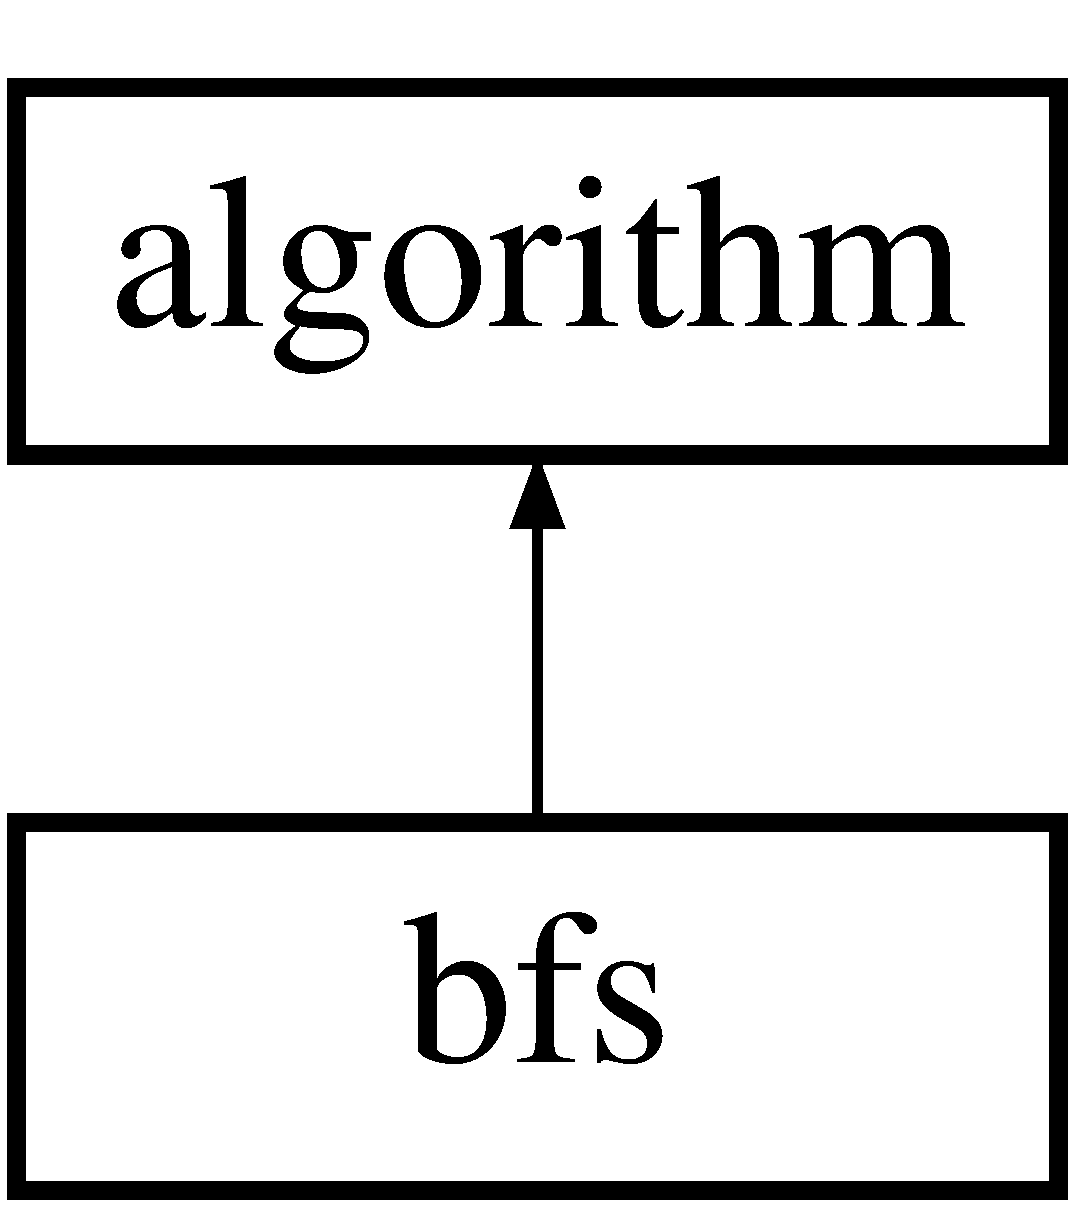
\includegraphics[height=2.000000cm]{classbfs}
\end{center}
\end{figure}
\subsection*{Public Types}
\begin{DoxyCompactItemize}
\item 
\mbox{\Hypertarget{classbfs_aa0b58a03ca2fc32117948ab27a806bd1}\label{classbfs_aa0b58a03ca2fc32117948ab27a806bd1}} 
typedef list$<$ \mbox{\hyperlink{classedge}{edge}} $>$\+::const\+\_\+iterator \mbox{\hyperlink{classbfs_aa0b58a03ca2fc32117948ab27a806bd1}{tree\+\_\+edges\+\_\+iterator}}
\begin{DoxyCompactList}\small\item\em Iterator for tree-\/edges. \end{DoxyCompactList}\item 
\mbox{\Hypertarget{classbfs_acafce54954100cc7bc9f80eb318a7bee}\label{classbfs_acafce54954100cc7bc9f80eb318a7bee}} 
typedef list$<$ \mbox{\hyperlink{classnode}{node}} $>$\+::const\+\_\+iterator \mbox{\hyperlink{classbfs_acafce54954100cc7bc9f80eb318a7bee}{bfs\+\_\+iterator}}
\begin{DoxyCompactList}\small\item\em Iterator for nodes in B\+F\+S-\/order. \end{DoxyCompactList}\item 
\mbox{\Hypertarget{classbfs_aecd86c7c1f1086d4b6b11c2a0eb12afe}\label{classbfs_aecd86c7c1f1086d4b6b11c2a0eb12afe}} 
typedef list$<$ \mbox{\hyperlink{classedge}{edge}} $>$\+::const\+\_\+iterator \mbox{\hyperlink{classbfs_aecd86c7c1f1086d4b6b11c2a0eb12afe}{non\+\_\+tree\+\_\+edges\+\_\+iterator}}
\begin{DoxyCompactList}\small\item\em Iterator for non-\/tree-\/edges. \end{DoxyCompactList}\item 
\mbox{\Hypertarget{classbfs_a386ac6f3c63e38c3f5263e15c3ab9d01}\label{classbfs_a386ac6f3c63e38c3f5263e15c3ab9d01}} 
typedef list$<$ \mbox{\hyperlink{classbfs_acafce54954100cc7bc9f80eb318a7bee}{bfs\+\_\+iterator}} $>$\+::const\+\_\+iterator \mbox{\hyperlink{classbfs_a386ac6f3c63e38c3f5263e15c3ab9d01}{roots\+\_\+iterator}}
\begin{DoxyCompactList}\small\item\em Iterator for roots of trees in B\+F\+S-\/forest. \end{DoxyCompactList}\end{DoxyCompactItemize}
\subsection*{Public Member Functions}
\begin{DoxyCompactItemize}
\item 
\mbox{\Hypertarget{classbfs_a16543f987ad29303e7d13650d5463605}\label{classbfs_a16543f987ad29303e7d13650d5463605}} 
\mbox{\hyperlink{classbfs_a16543f987ad29303e7d13650d5463605}{bfs}} ()
\begin{DoxyCompactList}\small\item\em Constructor. \end{DoxyCompactList}\item 
\mbox{\Hypertarget{classbfs_a6999a08f3cee2b54f07ffeac0d484df1}\label{classbfs_a6999a08f3cee2b54f07ffeac0d484df1}} 
virtual \mbox{\hyperlink{classbfs_a6999a08f3cee2b54f07ffeac0d484df1}{$\sim$bfs}} ()
\begin{DoxyCompactList}\small\item\em Destructor. \end{DoxyCompactList}\item 
auto \+\_\+\+\_\+cdecl \mbox{\hyperlink{classbfs_aaeebfe1628febd8d4ba658efc0ef51ed}{run}} (\mbox{\hyperlink{classgraph}{graph}} \&G) -\/$>$ int
\begin{DoxyCompactList}\small\item\em Applies algorithm to graph g. \end{DoxyCompactList}\item 
virtual auto \+\_\+\+\_\+cdecl \mbox{\hyperlink{classbfs_a57bc562775d63c4bbec63ee403e0fde7}{check}} (\mbox{\hyperlink{classgraph}{graph}} \&G) -\/$>$ int
\begin{DoxyCompactList}\small\item\em Checks whether the preconditions for B\+FS are satisfied. \end{DoxyCompactList}\item 
virtual auto \+\_\+\+\_\+cdecl \mbox{\hyperlink{classbfs_a9f93abba43ea1fa130a4c26b32793f2f}{reset}} () -\/$>$ void
\begin{DoxyCompactList}\small\item\em Resets algorithm. \end{DoxyCompactList}\item 
auto \+\_\+\+\_\+cdecl \mbox{\hyperlink{classbfs_aecb495d5cc06f8a0f89239d70668abba}{start\+\_\+node}} (const \mbox{\hyperlink{classnode}{node}} \&n) -\/$>$ void
\begin{DoxyCompactList}\small\item\em Sets start-\/node for B\+FS. \end{DoxyCompactList}\item 
auto \+\_\+\+\_\+cdecl \mbox{\hyperlink{classbfs_a80a7ae50880684eb261e7e8e807645ef}{start\+\_\+node}} () const -\/$>$ \mbox{\hyperlink{classnode}{node}}
\begin{DoxyCompactList}\small\item\em Returns start-\/node for B\+FS. \end{DoxyCompactList}\item 
auto \+\_\+\+\_\+cdecl \mbox{\hyperlink{classbfs_ac58d930764e6aa859fe706b1d916b9ad}{scan\+\_\+whole\+\_\+graph}} (bool set) -\/$>$ void
\begin{DoxyCompactList}\small\item\em Enables or disables scanning of the whole graph. \end{DoxyCompactList}\item 
auto \+\_\+\+\_\+cdecl \mbox{\hyperlink{classbfs_a558df71124787874724d67eeace62022}{scan\+\_\+whole\+\_\+graph}} () const -\/$>$ void
\begin{DoxyCompactList}\small\item\em Returns whether the whole graph will be scanned. \end{DoxyCompactList}\item 
auto \+\_\+\+\_\+cdecl \mbox{\hyperlink{classbfs_aa02df0b00c5fbaa29b9a41a211732e0f}{calc\+\_\+level}} (bool set) -\/$>$ void
\begin{DoxyCompactList}\small\item\em Enables or disables the calculation of level-\/numbers for each node. \end{DoxyCompactList}\item 
auto \+\_\+\+\_\+cdecl \mbox{\hyperlink{classbfs_a2d36d5c58653acfb219bed569e399a51}{calc\+\_\+level}} () const -\/$>$ bool
\begin{DoxyCompactList}\small\item\em Returns whether level-\/numbers will be calculated. \end{DoxyCompactList}\item 
auto \+\_\+\+\_\+cdecl \mbox{\hyperlink{classbfs_afed1aa751dbea4b6fb9dbdcea24b04f2}{store\+\_\+non\+\_\+tree\+\_\+edges}} (bool set) -\/$>$ void
\begin{DoxyCompactList}\small\item\em Enables or disables the storing of non-\/tree-\/edges. \end{DoxyCompactList}\item 
auto \+\_\+\+\_\+cdecl \mbox{\hyperlink{classbfs_a9c0188bc1f5a26aa48201640adcaa078}{store\+\_\+non\+\_\+tree\+\_\+edges}} () const -\/$>$ bool
\begin{DoxyCompactList}\small\item\em Returns whether the storing of non-\/tree-\/edges is enabled. \end{DoxyCompactList}\item 
auto \+\_\+\+\_\+cdecl \mbox{\hyperlink{classbfs_aa7200a3b11a17b8c87675b1a9bc010aa}{store\+\_\+preds}} (bool set) -\/$>$ void
\begin{DoxyCompactList}\small\item\em Enables or disables the storing of predecessors. \end{DoxyCompactList}\item 
auto \+\_\+\+\_\+cdecl \mbox{\hyperlink{classbfs_add14dde492d4df084198ff2957c9b610}{store\+\_\+preds}} () const -\/$>$ bool
\begin{DoxyCompactList}\small\item\em Returns whether the storing of predecessors is enabled. \end{DoxyCompactList}\item 
auto \+\_\+\+\_\+cdecl \mbox{\hyperlink{classbfs_a589d9acf6d6aeeac5f586a5fdac6528e}{reached}} (const \mbox{\hyperlink{classnode}{node}} \&n) const -\/$>$ bool
\begin{DoxyCompactList}\small\item\em Checks whether node {\itshape n} was reached in B\+FS. \end{DoxyCompactList}\item 
auto \+\_\+\+\_\+cdecl \mbox{\hyperlink{classbfs_aa7e557aefbff0b1308462d9b31ae3de1}{bfs\+\_\+num}} (const \mbox{\hyperlink{classnode}{node}} \&n) const -\/$>$ int
\begin{DoxyCompactList}\small\item\em B\+F\+S-\/number of {\itshape n}. \end{DoxyCompactList}\item 
auto \+\_\+\+\_\+cdecl \mbox{\hyperlink{classbfs_a8cd9e96931e8b8c087f962eb9323dac4}{operator\mbox{[}$\,$\mbox{]}}} (const \mbox{\hyperlink{classnode}{node}} \&n) const -\/$>$ int
\begin{DoxyCompactList}\small\item\em B\+F\+S-\/number of {\itshape n}. \end{DoxyCompactList}\item 
auto \+\_\+\+\_\+cdecl \mbox{\hyperlink{classbfs_a9c2effb945b67f73b3abe33682df139f}{level}} (const \mbox{\hyperlink{classnode}{node}} \&n) const -\/$>$ int
\begin{DoxyCompactList}\small\item\em Level-\/number of node {\itshape n}. \end{DoxyCompactList}\item 
auto \+\_\+\+\_\+cdecl \mbox{\hyperlink{classbfs_ab8a8b65048c4ffb6caa7651b793e4e56}{father}} (const \mbox{\hyperlink{classnode}{node}} \&n) const -\/$>$ \mbox{\hyperlink{classnode}{node}}
\begin{DoxyCompactList}\small\item\em Father of node {\itshape n} in B\+F\+S-\/forest. \end{DoxyCompactList}\item 
auto \+\_\+\+\_\+cdecl \mbox{\hyperlink{classbfs_aef8c6f063e1d1e52770f5adf12c7cb28}{tree\+\_\+edges\+\_\+begin}} () const -\/$>$ \mbox{\hyperlink{classbfs_aa0b58a03ca2fc32117948ab27a806bd1}{tree\+\_\+edges\+\_\+iterator}}
\begin{DoxyCompactList}\small\item\em Iterate through all tree-\/edges of last B\+FS. \end{DoxyCompactList}\item 
auto \+\_\+\+\_\+cdecl \mbox{\hyperlink{classbfs_a55e57b15957b08f3334568eeefb4223a}{tree\+\_\+edges\+\_\+end}} () const -\/$>$ \mbox{\hyperlink{classbfs_aa0b58a03ca2fc32117948ab27a806bd1}{tree\+\_\+edges\+\_\+iterator}}
\begin{DoxyCompactList}\small\item\em End-\/iterator for iteration through all tree-\/edges picked of last B\+FS. \end{DoxyCompactList}\item 
auto \+\_\+\+\_\+cdecl \mbox{\hyperlink{classbfs_a350eb3e4fcfea5c9c9cd18f54a722289}{begin}} () const -\/$>$ \mbox{\hyperlink{classbfs_acafce54954100cc7bc9f80eb318a7bee}{bfs\+\_\+iterator}}
\begin{DoxyCompactList}\small\item\em Iterate through all (reached) nodes in B\+F\+S-\/\+Order. \end{DoxyCompactList}\item 
auto \+\_\+\+\_\+cdecl \mbox{\hyperlink{classbfs_a355a37450bce8f14548983d5c6097aea}{end}} () const -\/$>$ \mbox{\hyperlink{classbfs_acafce54954100cc7bc9f80eb318a7bee}{bfs\+\_\+iterator}}
\begin{DoxyCompactList}\small\item\em End-\/iterator for iteration through all (reached) nodes in B\+F\+S-\/\+Order. \end{DoxyCompactList}\item 
auto \+\_\+\+\_\+cdecl \mbox{\hyperlink{classbfs_a15d846159cfe9524081ad318fb72661f}{non\+\_\+tree\+\_\+edges\+\_\+begin}} () const -\/$>$ \mbox{\hyperlink{classbfs_aecd86c7c1f1086d4b6b11c2a0eb12afe}{non\+\_\+tree\+\_\+edges\+\_\+iterator}}
\begin{DoxyCompactList}\small\item\em Iterate through all non-\/tree-\/edges (if enabled). \end{DoxyCompactList}\item 
auto \+\_\+\+\_\+cdecl \mbox{\hyperlink{classbfs_ae4d59095371f625a831de4262ab16d31}{non\+\_\+tree\+\_\+edges\+\_\+end}} () const -\/$>$ \mbox{\hyperlink{classbfs_aecd86c7c1f1086d4b6b11c2a0eb12afe}{non\+\_\+tree\+\_\+edges\+\_\+iterator}}
\begin{DoxyCompactList}\small\item\em End-\/iterator for iteration through all non-\/tree-\/edges (if enabled). \end{DoxyCompactList}\item 
auto \+\_\+\+\_\+cdecl \mbox{\hyperlink{classbfs_a8ba1e13916302d68faafc5c5098b04fe}{roots\+\_\+begin}} () const -\/$>$ \mbox{\hyperlink{classbfs_a386ac6f3c63e38c3f5263e15c3ab9d01}{roots\+\_\+iterator}}
\begin{DoxyCompactList}\small\item\em Iterator pointing towards the first root in the B\+F\+S-\/forest. \end{DoxyCompactList}\item 
auto \+\_\+\+\_\+cdecl \mbox{\hyperlink{classbfs_ab120a4a529a9cbf407e5dcba8d33598e}{roots\+\_\+end}} () const -\/$>$ \mbox{\hyperlink{classbfs_a386ac6f3c63e38c3f5263e15c3ab9d01}{roots\+\_\+iterator}}
\begin{DoxyCompactList}\small\item\em Iterator pointing to the end of all roots. \end{DoxyCompactList}\item 
auto \+\_\+\+\_\+cdecl \mbox{\hyperlink{classbfs_a98b86a661aa5284b77c260908f0872a0}{number\+\_\+of\+\_\+reached\+\_\+nodes}} () const -\/$>$ int
\begin{DoxyCompactList}\small\item\em Number of nodes reached in last B\+FS. \end{DoxyCompactList}\item 
virtual auto \+\_\+\+\_\+cdecl \mbox{\hyperlink{classbfs_a5f6e0f575ee3d851ffbb24bdda90ed85}{init\+\_\+handler}} (\mbox{\hyperlink{classgraph}{graph}} \&G) -\/$>$ void
\begin{DoxyCompactList}\small\item\em Called at the start of B\+FS. \end{DoxyCompactList}\item 
virtual auto \+\_\+\+\_\+cdecl \mbox{\hyperlink{classbfs_a6c31ed93b4646218a90ded9ef7bb8366}{end\+\_\+handler}} (\mbox{\hyperlink{classgraph}{graph}} \&G) -\/$>$ void
\begin{DoxyCompactList}\small\item\em Called right before the end of B\+FS. \end{DoxyCompactList}\item 
virtual auto \+\_\+\+\_\+cdecl \mbox{\hyperlink{classbfs_a4ae61f9bbdfddf3f3a8b083e1aed9eeb}{popped\+\_\+node\+\_\+handler}} (\mbox{\hyperlink{classgraph}{graph}} \&G, \mbox{\hyperlink{classnode}{node}} \&n) -\/$>$ void
\begin{DoxyCompactList}\small\item\em Called after the node {\itshape n} was taken out of the queue. \end{DoxyCompactList}\item 
virtual auto \+\_\+\+\_\+cdecl \mbox{\hyperlink{classbfs_a4543e9eb32673c20271baea923340ab3}{finished\+\_\+node\+\_\+handler}} (\mbox{\hyperlink{classgraph}{graph}} \&G, \mbox{\hyperlink{classnode}{node}} \&n) -\/$>$ void
\begin{DoxyCompactList}\small\item\em Called when finished with the node {\itshape n}. \end{DoxyCompactList}\item 
virtual auto \+\_\+\+\_\+cdecl \mbox{\hyperlink{classbfs_a39cda7554a4ddce1331af32271904faa}{unused\+\_\+node\+\_\+handler}} (\mbox{\hyperlink{classgraph}{graph}} \&G, \mbox{\hyperlink{classnode}{node}} \&n, \mbox{\hyperlink{classnode}{node}} \&f) -\/$>$ void
\begin{DoxyCompactList}\small\item\em Called when an unused node {\itshape n} was discovered. \end{DoxyCompactList}\item 
virtual auto \+\_\+\+\_\+cdecl \mbox{\hyperlink{classbfs_a85beb51af51c14a193b3cbf09e2aa9fc}{used\+\_\+node\+\_\+handler}} (\mbox{\hyperlink{classgraph}{graph}} \&G, \mbox{\hyperlink{classnode}{node}} \&n, \mbox{\hyperlink{classnode}{node}} \&f) -\/$>$ void
\begin{DoxyCompactList}\small\item\em Called when an used node {\itshape n} was found. \end{DoxyCompactList}\item 
virtual auto \+\_\+\+\_\+cdecl \mbox{\hyperlink{classbfs_ab4b0ac22769cedc2a45e72efb3dd5565}{new\+\_\+start\+\_\+handler}} (\mbox{\hyperlink{classgraph}{graph}} \&G, \mbox{\hyperlink{classnode}{node}} \&n) -\/$>$ void
\begin{DoxyCompactList}\small\item\em Called when B\+FS is started with start-\/node {\itshape n}. \end{DoxyCompactList}\end{DoxyCompactItemize}
\subsection*{Protected Attributes}
\begin{DoxyCompactItemize}
\item 
\mbox{\Hypertarget{classbfs_a5a4adad9562896536b8b58ab237e8478}\label{classbfs_a5a4adad9562896536b8b58ab237e8478}} 
int \mbox{\hyperlink{classbfs_a5a4adad9562896536b8b58ab237e8478}{act\+\_\+bfs\+\_\+num}}
\begin{DoxyCompactList}\small\item\em B\+FS number that will be assigned next. \end{DoxyCompactList}\item 
\mbox{\Hypertarget{classbfs_aff965242124a7e3a6308de0c0ebfa741}\label{classbfs_aff965242124a7e3a6308de0c0ebfa741}} 
deque$<$ \mbox{\hyperlink{classnode}{node}} $>$ \mbox{\hyperlink{classbfs_aff965242124a7e3a6308de0c0ebfa741}{qu}}
\begin{DoxyCompactList}\small\item\em queue used in B\+FS. \end{DoxyCompactList}\item 
list$<$ \mbox{\hyperlink{classnode}{node}} $>$ \mbox{\hyperlink{classbfs_a35b0acd44887615142fd5f2fc6197452}{bfs\+\_\+order}}
\begin{DoxyCompactList}\small\item\em List of nodes in B\+F\+S-\/order. \end{DoxyCompactList}\item 
list$<$ \mbox{\hyperlink{classedge}{edge}} $>$ \mbox{\hyperlink{classbfs_aa259f09ada9928cda41bcb540f685e80}{tree}}
\begin{DoxyCompactList}\small\item\em List of all edges of the B\+F\+S-\/tree. \end{DoxyCompactList}\item 
\mbox{\Hypertarget{classbfs_a59d0c5c5ad2715776b20b1aec03dbc3a}\label{classbfs_a59d0c5c5ad2715776b20b1aec03dbc3a}} 
\mbox{\hyperlink{classnode__map}{node\+\_\+map}}$<$ int $>$ \mbox{\hyperlink{classbfs_a59d0c5c5ad2715776b20b1aec03dbc3a}{bfs\+\_\+number}}
\begin{DoxyCompactList}\small\item\em Stores B\+F\+S-\/number of nodes. \end{DoxyCompactList}\item 
\mbox{\Hypertarget{classbfs_ac3db80b59d5db049199936445a6c2da8}\label{classbfs_ac3db80b59d5db049199936445a6c2da8}} 
int \mbox{\hyperlink{classbfs_ac3db80b59d5db049199936445a6c2da8}{reached\+\_\+nodes}}
\begin{DoxyCompactList}\small\item\em Number of nodes reached so far. \end{DoxyCompactList}\item 
list$<$ \mbox{\hyperlink{classbfs_acafce54954100cc7bc9f80eb318a7bee}{bfs\+\_\+iterator}} $>$ \mbox{\hyperlink{classbfs_a79d19028002766f7992fe94689217f99}{roots}}
\begin{DoxyCompactList}\small\item\em List of all roots of the B\+F\+S-\/tree. \end{DoxyCompactList}\item 
bool \mbox{\hyperlink{classbfs_a6c08fbcc90d71f1cbdd03a1cdaa9dc99}{whole\+\_\+graph}}
\begin{DoxyCompactList}\small\item\em Stores whether whole graph will be scanned. \end{DoxyCompactList}\item 
\mbox{\hyperlink{classnode}{node}} \mbox{\hyperlink{classbfs_af2ab561d9e60a9fc2e25b02d1f807f96}{start}}
\begin{DoxyCompactList}\small\item\em Stores start node. \end{DoxyCompactList}\item 
\mbox{\hyperlink{classnode__map}{node\+\_\+map}}$<$ int $>$ $\ast$ \mbox{\hyperlink{classbfs_aab92e9d128612c28324aafe4750dbc84}{level\+\_\+number}}
\begin{DoxyCompactList}\small\item\em Stores level number of each node (if enabled) \end{DoxyCompactList}\item 
list$<$ \mbox{\hyperlink{classedge}{edge}} $>$ $\ast$ \mbox{\hyperlink{classbfs_aa6783e3e2ac4235403b37df3ee3ee968}{non\+\_\+tree}}
\begin{DoxyCompactList}\small\item\em List of non-\/tree edges (if enabled) \end{DoxyCompactList}\item 
\mbox{\hyperlink{classnode__map}{node\+\_\+map}}$<$ \mbox{\hyperlink{classnode}{node}} $>$ $\ast$ \mbox{\hyperlink{classbfs_a3bac5ed333bb78a30a67099c3b94aa0c}{preds}}
\begin{DoxyCompactList}\small\item\em Stores father of each node (if enabled) \end{DoxyCompactList}\end{DoxyCompactItemize}


\subsection{Detailed Description}
Breadth-\/\+First-\/\+Search (B\+FS) algorithm. 

\begin{DoxyParagraph}{Date}
2019/05/07 15\+:58\+:54 
\end{DoxyParagraph}
\begin{DoxyParagraph}{Revision}
1.\+14 
\end{DoxyParagraph}


Encapsulates the B\+FS algorithm together with all data produced by it. There are a few parameters, which on the one hand influence the behaviour of B\+FS (e.\+g. \mbox{\hyperlink{classbfs_aecb495d5cc06f8a0f89239d70668abba}{bfs\+::start\+\_\+node}}) and on the other hand toggle the storing of extra information, such as the level-\/number of each node. In detail these are\+:
\begin{DoxyItemize}
\item \mbox{\hyperlink{classbfs_aecb495d5cc06f8a0f89239d70668abba}{bfs\+::start\+\_\+node}} (default\+: an arbitrary node will be chosen)
\item \mbox{\hyperlink{classbfs_ac58d930764e6aa859fe706b1d916b9ad}{bfs\+::scan\+\_\+whole\+\_\+graph}} states whether B\+FS will be continued in the unused part of the graph, if not all nodes were touched at the end of B\+FS started at the start-\/node. (default\+: disabled)
\item \mbox{\hyperlink{classbfs_aa02df0b00c5fbaa29b9a41a211732e0f}{bfs\+::calc\+\_\+level}} toggle storing of level-\/numbers for each node, i.\+e. its distance from the start-\/node. (default\+: disabled)
\item \mbox{\hyperlink{classbfs_aa7200a3b11a17b8c87675b1a9bc010aa}{bfs\+::store\+\_\+preds}} toggle storing the predecessor of each node, i.\+e. the father in the B\+F\+S-\/tree. (default\+: disabled)
\item \mbox{\hyperlink{classbfs_afed1aa751dbea4b6fb9dbdcea24b04f2}{bfs\+::store\+\_\+non\+\_\+tree\+\_\+edges}} toggle storing of all non\+\_\+tree\+\_\+edges (tree\+\_\+edges are always stored) in a list and thus enable or disable iteration through all non\+\_\+tree\+\_\+edges. (default\+: disabled)
\end{DoxyItemize}

{\itshape Please} {\itshape note} that the algorithm always starts with the given start-\/node (if none was given, the first node is chosen and stored, thus after B\+FS the root of the tree is always accesible via \mbox{\hyperlink{classbfs_aecb495d5cc06f8a0f89239d70668abba}{bfs\+::start\+\_\+node}}) and continues until no more unused nodes are reachable from already used ones. Thus if the graph isn\textquotesingle{}t connected not {\itshape all} nodes will be reached. If \mbox{\hyperlink{classbfs_ac58d930764e6aa859fe706b1d916b9ad}{bfs\+::scan\+\_\+whole\+\_\+graph}} isn\textquotesingle{}t set the B\+FS stops here. If it is set, the B\+FS will be continued with the next unused node and so on until all nodes were used.

For further customization a few virtual functions, so called handler, are called at crucial stages of the algorithm. In this basic implementation all of these handler are empty. So if one wants to add only a few lines of code (e.\+g. some new numbering) he is likely to take this class as base-\/class and override the handler where neccessary. In detail these are (please look at the source code to see where they are called)\+:
\begin{DoxyItemize}
\item \mbox{\hyperlink{classbfs_a5f6e0f575ee3d851ffbb24bdda90ed85}{bfs\+::init\+\_\+handler}}
\item \mbox{\hyperlink{classbfs_a6c31ed93b4646218a90ded9ef7bb8366}{bfs\+::end\+\_\+handler}}
\item \mbox{\hyperlink{classbfs_a4ae61f9bbdfddf3f3a8b083e1aed9eeb}{bfs\+::popped\+\_\+node\+\_\+handler}}
\item \mbox{\hyperlink{classbfs_a4543e9eb32673c20271baea923340ab3}{bfs\+::finished\+\_\+node\+\_\+handler}}
\item \mbox{\hyperlink{classbfs_a39cda7554a4ddce1331af32271904faa}{bfs\+::unused\+\_\+node\+\_\+handler}}
\item \mbox{\hyperlink{classbfs_a85beb51af51c14a193b3cbf09e2aa9fc}{bfs\+::used\+\_\+node\+\_\+handler}}
\item \mbox{\hyperlink{classbfs_ab4b0ac22769cedc2a45e72efb3dd5565}{bfs\+::new\+\_\+start\+\_\+handler}}
\end{DoxyItemize}

{\itshape Please} {\itshape note\+:} We do {\itshape not} claim that the set of handlers provided is sufficient in any way. So if you believe that some new handler is needed urgently please let us know.

There is a lot of information stored during B\+FS (e.\+g. nodes in bfs-\/order, list of non-\/tree edges). Some of it can be obtained directly by using the corresponding member-\/function (e.\+g. \mbox{\hyperlink{classbfs_aa7e557aefbff0b1308462d9b31ae3de1}{bfs\+::bfs\+\_\+num}}), but all information that can be thought of as a list (e.\+g. nodes in bfs-\/order) can be accessed through iterators. In detail these are (of course depending on what options are chosen!)\+:
\begin{DoxyItemize}
\item \mbox{\hyperlink{classbfs_acafce54954100cc7bc9f80eb318a7bee}{bfs\+::bfs\+\_\+iterator}}
\item \mbox{\hyperlink{classbfs_aa0b58a03ca2fc32117948ab27a806bd1}{bfs\+::tree\+\_\+edges\+\_\+iterator}}
\item \mbox{\hyperlink{classbfs_aecd86c7c1f1086d4b6b11c2a0eb12afe}{bfs\+::non\+\_\+tree\+\_\+edges\+\_\+iterator}}
\item \mbox{\hyperlink{classbfs_a386ac6f3c63e38c3f5263e15c3ab9d01}{bfs\+::roots\+\_\+iterator}} 
\end{DoxyItemize}

\subsection{Member Function Documentation}
\mbox{\Hypertarget{classbfs_a350eb3e4fcfea5c9c9cd18f54a722289}\label{classbfs_a350eb3e4fcfea5c9c9cd18f54a722289}} 
\index{bfs@{bfs}!begin@{begin}}
\index{begin@{begin}!bfs@{bfs}}
\subsubsection{\texorpdfstring{begin()}{begin()}}
{\footnotesize\ttfamily auto \+\_\+\+\_\+cdecl bfs\+::begin (\begin{DoxyParamCaption}{ }\end{DoxyParamCaption}) const -\/$>$ \mbox{\hyperlink{classbfs_acafce54954100cc7bc9f80eb318a7bee}{bfs\+\_\+iterator}}
	\hspace{0.3cm}{\ttfamily [inline]}}



Iterate through all (reached) nodes in B\+F\+S-\/\+Order. 

\begin{DoxyReturn}{Returns}
Start for iteration through all nodes in B\+F\+S-\/order. 
\end{DoxyReturn}
\mbox{\Hypertarget{classbfs_aa7e557aefbff0b1308462d9b31ae3de1}\label{classbfs_aa7e557aefbff0b1308462d9b31ae3de1}} 
\index{bfs@{bfs}!bfs\+\_\+num@{bfs\+\_\+num}}
\index{bfs\+\_\+num@{bfs\+\_\+num}!bfs@{bfs}}
\subsubsection{\texorpdfstring{bfs\+\_\+num()}{bfs\_num()}}
{\footnotesize\ttfamily auto \+\_\+\+\_\+cdecl bfs\+::bfs\+\_\+num (\begin{DoxyParamCaption}\item[{const \mbox{\hyperlink{classnode}{node}} \&}]{n }\end{DoxyParamCaption}) const -\/$>$ int
	\hspace{0.3cm}{\ttfamily [inline]}}



B\+F\+S-\/number of {\itshape n}. 

{\itshape Please} {\itshape note} that B\+F\+S-\/number 0 means that this node wasn\textquotesingle{}t reached.


\begin{DoxyParams}{Parameters}
{\em n} & node. \\
\hline
\end{DoxyParams}
\begin{DoxyReturn}{Returns}
B\+F\+S-\/number of {\itshape n}. 
\end{DoxyReturn}
\mbox{\Hypertarget{classbfs_aa02df0b00c5fbaa29b9a41a211732e0f}\label{classbfs_aa02df0b00c5fbaa29b9a41a211732e0f}} 
\index{bfs@{bfs}!calc\+\_\+level@{calc\+\_\+level}}
\index{calc\+\_\+level@{calc\+\_\+level}!bfs@{bfs}}
\subsubsection{\texorpdfstring{calc\+\_\+level()}{calc\_level()}\hspace{0.1cm}{\footnotesize\ttfamily [1/2]}}
{\footnotesize\ttfamily void bfs\+::calc\+\_\+level (\begin{DoxyParamCaption}\item[{bool}]{set }\end{DoxyParamCaption}) -\/$>$ void}



Enables or disables the calculation of level-\/numbers for each node. 

If enabled each node gets a level-\/number, i.\+e. its distance from the start-\/node.


\begin{DoxyParams}{Parameters}
{\em set} & if true level-\/number will be calculated. \\
\hline
\end{DoxyParams}
\begin{DoxySeeAlso}{See also}
\mbox{\hyperlink{classbfs_a9c2effb945b67f73b3abe33682df139f}{bfs\+::level}} 
\end{DoxySeeAlso}
\mbox{\Hypertarget{classbfs_a2d36d5c58653acfb219bed569e399a51}\label{classbfs_a2d36d5c58653acfb219bed569e399a51}} 
\index{bfs@{bfs}!calc\+\_\+level@{calc\+\_\+level}}
\index{calc\+\_\+level@{calc\+\_\+level}!bfs@{bfs}}
\subsubsection{\texorpdfstring{calc\+\_\+level()}{calc\_level()}\hspace{0.1cm}{\footnotesize\ttfamily [2/2]}}
{\footnotesize\ttfamily auto \+\_\+\+\_\+cdecl bfs\+::calc\+\_\+level (\begin{DoxyParamCaption}{ }\end{DoxyParamCaption}) const -\/$>$ bool \hspace{0.3cm}{\ttfamily [inline]}}



Returns whether level-\/numbers will be calculated. 


\begin{DoxyRetVals}{Return values}
{\em true} & iff level-\/numbers will be calculated. \\
\hline
\end{DoxyRetVals}
\begin{DoxySeeAlso}{See also}
\mbox{\hyperlink{classbfs_a9c2effb945b67f73b3abe33682df139f}{bfs\+::level}} 
\end{DoxySeeAlso}
\mbox{\Hypertarget{classbfs_a57bc562775d63c4bbec63ee403e0fde7}\label{classbfs_a57bc562775d63c4bbec63ee403e0fde7}} 
\index{bfs@{bfs}!check@{check}}
\index{check@{check}!bfs@{bfs}}
\subsubsection{\texorpdfstring{check()}{check()}}
{\footnotesize\ttfamily virtual auto \+\_\+\+\_\+cdecl bfs\+::check (\begin{DoxyParamCaption}\item[{\mbox{\hyperlink{classgraph}{graph}} \&}]{G }\end{DoxyParamCaption}) -\/$>$ int \hspace{0.3cm}{\ttfamily [inline]}, {\ttfamily [virtual]}}



Checks whether the preconditions for B\+FS are satisfied. 

Currently there aren\textquotesingle{}t any restricitions for the B\+FS algorithm.


\begin{DoxyParams}{Parameters}
{\em G} & graph. \\
\hline
\end{DoxyParams}

\begin{DoxyRetVals}{Return values}
{\em \mbox{\hyperlink{classalgorithm_af1a0078e153aa99c24f9bdf0d97f6710aae4c1cd7fe8d8cf4b143241a6e7c31cf}{algorithm\+::\+K\+G\+L\+\_\+\+OK}}} & if algorithm can be applied \\
\hline
{\em \mbox{\hyperlink{classalgorithm_af1a0078e153aa99c24f9bdf0d97f6710ae67bf27b2ef31f73e545a7f9f4a69556}{algorithm\+::\+K\+G\+L\+\_\+\+E\+R\+R\+OR}}} & otherwise. \\
\hline
\end{DoxyRetVals}


Implements \mbox{\hyperlink{classalgorithm_a05c0f25463eb35a77b2d73fc06bb2c0e}{algorithm}}.

\mbox{\Hypertarget{classbfs_a355a37450bce8f14548983d5c6097aea}\label{classbfs_a355a37450bce8f14548983d5c6097aea}} 
\index{bfs@{bfs}!end@{end}}
\index{end@{end}!bfs@{bfs}}
\subsubsection{\texorpdfstring{end()}{end()}}
{\footnotesize\ttfamily auto \+\_\+\+\_\+cdecl bfs\+::end (\begin{DoxyParamCaption}{ }\end{DoxyParamCaption}) const -\/$>$ \mbox{\hyperlink{classbfs_acafce54954100cc7bc9f80eb318a7bee}{bfs\+\_\+iterator}}
	\hspace{0.3cm}{\ttfamily [inline]}}



End-\/iterator for iteration through all (reached) nodes in B\+F\+S-\/\+Order. 

\begin{DoxyReturn}{Returns}
End for iteration through all (reached) nodes 
\end{DoxyReturn}
\mbox{\Hypertarget{classbfs_a6c31ed93b4646218a90ded9ef7bb8366}\label{classbfs_a6c31ed93b4646218a90ded9ef7bb8366}} 
\index{bfs@{bfs}!end\+\_\+handler@{end\+\_\+handler}}
\index{end\+\_\+handler@{end\+\_\+handler}!bfs@{bfs}}
\subsubsection{\texorpdfstring{end\+\_\+handler()}{end\_handler()}}
{\footnotesize\ttfamily virtual auto \+\_\+\+\_\+cdecl bfs\+::end\+\_\+handler (\begin{DoxyParamCaption}\item[{\mbox{\hyperlink{classgraph}{graph}} \&}]{G }\end{DoxyParamCaption}) -\/$>$ void \hspace{0.3cm}{\ttfamily [inline]}, {\ttfamily [virtual]}}



Called right before the end of B\+FS. 


\begin{DoxyParams}{Parameters}
{\em G} & graph for which B\+FS was invoked. \\
\hline
\end{DoxyParams}
\mbox{\Hypertarget{classbfs_ab8a8b65048c4ffb6caa7651b793e4e56}\label{classbfs_ab8a8b65048c4ffb6caa7651b793e4e56}} 
\index{bfs@{bfs}!father@{father}}
\index{father@{father}!bfs@{bfs}}
\subsubsection{\texorpdfstring{father()}{father()}}
{\footnotesize\ttfamily auto \+\_\+\+\_\+cdecl bfs\+::father (\begin{DoxyParamCaption}\item[{const \mbox{\hyperlink{classnode}{node}} \&}]{n }\end{DoxyParamCaption}) const -\/$>$ \mbox{\hyperlink{classnode}{node}}
	\hspace{0.3cm}{\ttfamily [inline]}}



Father of node {\itshape n} in B\+F\+S-\/forest. 

If {\itshape n} is a root in the forest or wasn\textquotesingle{}t reached the return value is the invalid node \mbox{\hyperlink{classnode_ad603259398d5667e3b97a6322a2bcc20}{node\+::node()}}. ~\newline
 {\itshape Please} {\itshape note} that this requires that this option was enabled during last run.


\begin{DoxyParams}{Parameters}
{\em n} & node. \\
\hline
\end{DoxyParams}
\begin{DoxyReturn}{Returns}
Father of {\itshape n}. 
\end{DoxyReturn}
\begin{DoxySeeAlso}{See also}
\mbox{\hyperlink{classbfs_aa7200a3b11a17b8c87675b1a9bc010aa}{bfs\+::store\+\_\+preds}} 
\end{DoxySeeAlso}
\mbox{\Hypertarget{classbfs_a4543e9eb32673c20271baea923340ab3}\label{classbfs_a4543e9eb32673c20271baea923340ab3}} 
\index{bfs@{bfs}!finished\+\_\+node\+\_\+handler@{finished\+\_\+node\+\_\+handler}}
\index{finished\+\_\+node\+\_\+handler@{finished\+\_\+node\+\_\+handler}!bfs@{bfs}}
\subsubsection{\texorpdfstring{finished\+\_\+node\+\_\+handler()}{finished\_node\_handler()}}
{\footnotesize\ttfamily virtual auto \+\_\+\+\_\+cdecl bfs\+::finished\+\_\+node\+\_\+handler (\begin{DoxyParamCaption}\item[{\mbox{\hyperlink{classgraph}{graph}} \&}]{G,  }\item[{\mbox{\hyperlink{classnode}{node}} \&}]{n }\end{DoxyParamCaption}) -\/$>$ void \hspace{0.3cm}{\ttfamily [inline]}, {\ttfamily [virtual]}}



Called when finished with the node {\itshape n}. 

A node is finished after all its neighbors have been visited.


\begin{DoxyParams}{Parameters}
{\em G} & graph for which B\+FS was invoked. \\
\hline
{\em n} & finished node. \\
\hline
\end{DoxyParams}
\mbox{\Hypertarget{classbfs_a5f6e0f575ee3d851ffbb24bdda90ed85}\label{classbfs_a5f6e0f575ee3d851ffbb24bdda90ed85}} 
\index{bfs@{bfs}!init\+\_\+handler@{init\+\_\+handler}}
\index{init\+\_\+handler@{init\+\_\+handler}!bfs@{bfs}}
\subsubsection{\texorpdfstring{init\+\_\+handler()}{init\_handler()}}
{\footnotesize\ttfamily virtual auto \+\_\+\+\_\+cdecl bfs\+::init\+\_\+handler (\begin{DoxyParamCaption}\item[{\mbox{\hyperlink{classgraph}{graph}} \&}]{G }\end{DoxyParamCaption}) -\/$>$ void \hspace{0.3cm}{\ttfamily [inline]}, {\ttfamily [virtual]}}



Called at the start of B\+FS. 


\begin{DoxyParams}{Parameters}
{\em G} & graph for which B\+FS was invoked. \\
\hline
\end{DoxyParams}
\mbox{\Hypertarget{classbfs_a9c2effb945b67f73b3abe33682df139f}\label{classbfs_a9c2effb945b67f73b3abe33682df139f}} 
\index{bfs@{bfs}!level@{level}}
\index{level@{level}!bfs@{bfs}}
\subsubsection{\texorpdfstring{level()}{level()}}
{\footnotesize\ttfamily auto \+\_\+\+\_\+cdecl bfs\+::level (\begin{DoxyParamCaption}\item[{const \mbox{\hyperlink{classnode}{node}} \&}]{n }\end{DoxyParamCaption}) const -\/$>$ int
	\hspace{0.3cm}{\ttfamily [inline]}}



Level-\/number of node {\itshape n}. 

{\itshape Please} {\itshape note} that this requires that this option was enabled during last run.


\begin{DoxyParams}{Parameters}
{\em n} & node. \\
\hline
\end{DoxyParams}
\begin{DoxyReturn}{Returns}
level-\/number of {\itshape n}. 
\end{DoxyReturn}
\begin{DoxySeeAlso}{See also}
\mbox{\hyperlink{classbfs_aa02df0b00c5fbaa29b9a41a211732e0f}{bfs\+::calc\+\_\+level}} 
\end{DoxySeeAlso}
\mbox{\Hypertarget{classbfs_ab4b0ac22769cedc2a45e72efb3dd5565}\label{classbfs_ab4b0ac22769cedc2a45e72efb3dd5565}} 
\index{bfs@{bfs}!new\+\_\+start\+\_\+handler@{new\+\_\+start\+\_\+handler}}
\index{new\+\_\+start\+\_\+handler@{new\+\_\+start\+\_\+handler}!bfs@{bfs}}
\subsubsection{\texorpdfstring{new\+\_\+start\+\_\+handler()}{new\_start\_handler()}}
{\footnotesize\ttfamily virtual auto \+\_\+\+\_\+cdecl bfs\+::new\+\_\+start\+\_\+handler (\begin{DoxyParamCaption}\item[{\mbox{\hyperlink{classgraph}{graph}} \&}]{G,  }\item[{\mbox{\hyperlink{classnode}{node}} \&}]{n }\end{DoxyParamCaption}) -\/$>$ void \hspace{0.3cm}{\ttfamily [inline]}, {\ttfamily [virtual]}}



Called when B\+FS is started with start-\/node {\itshape n}. 

This is particularly useful when B\+FS was invoked with the {\ttfamily scan\+\_\+whole\+\_\+graph} option.


\begin{DoxyParams}{Parameters}
{\em G} & graph for which B\+FS was invoked. \\
\hline
{\em n} & start-\/node. \\
\hline
\end{DoxyParams}
\begin{DoxySeeAlso}{See also}
\mbox{\hyperlink{classbfs_ac58d930764e6aa859fe706b1d916b9ad}{bfs\+::scan\+\_\+whole\+\_\+graph}} 
\end{DoxySeeAlso}
\mbox{\Hypertarget{classbfs_a15d846159cfe9524081ad318fb72661f}\label{classbfs_a15d846159cfe9524081ad318fb72661f}} 
\index{bfs@{bfs}!non\+\_\+tree\+\_\+edges\+\_\+begin@{non\+\_\+tree\+\_\+edges\+\_\+begin}}
\index{non\+\_\+tree\+\_\+edges\+\_\+begin@{non\+\_\+tree\+\_\+edges\+\_\+begin}!bfs@{bfs}}
\subsubsection{\texorpdfstring{non\+\_\+tree\+\_\+edges\+\_\+begin()}{non\_tree\_edges\_begin()}}
{\footnotesize\ttfamily auto \+\_\+\+\_\+cdecl bfs\+::non\+\_\+tree\+\_\+edges\+\_\+begin (\begin{DoxyParamCaption}{ }\end{DoxyParamCaption}) const -\/$>$ \mbox{\hyperlink{classbfs_aecd86c7c1f1086d4b6b11c2a0eb12afe}{non\+\_\+tree\+\_\+edges\+\_\+iterator}}
	\hspace{0.3cm}{\ttfamily [inline]}}



Iterate through all non-\/tree-\/edges (if enabled). 

\begin{DoxyReturn}{Returns}
Start for iteration through all non-\/tree-\/edges. 
\end{DoxyReturn}
\begin{DoxySeeAlso}{See also}
\mbox{\hyperlink{classbfs_afed1aa751dbea4b6fb9dbdcea24b04f2}{bfs\+::store\+\_\+non\+\_\+tree\+\_\+edges}} 
\end{DoxySeeAlso}
\mbox{\Hypertarget{classbfs_ae4d59095371f625a831de4262ab16d31}\label{classbfs_ae4d59095371f625a831de4262ab16d31}} 
\index{bfs@{bfs}!non\+\_\+tree\+\_\+edges\+\_\+end@{non\+\_\+tree\+\_\+edges\+\_\+end}}
\index{non\+\_\+tree\+\_\+edges\+\_\+end@{non\+\_\+tree\+\_\+edges\+\_\+end}!bfs@{bfs}}
\subsubsection{\texorpdfstring{non\+\_\+tree\+\_\+edges\+\_\+end()}{non\_tree\_edges\_end()}}
{\footnotesize\ttfamily auto \+\_\+\+\_\+cdecl bfs\+::non\+\_\+tree\+\_\+edges\+\_\+end (\begin{DoxyParamCaption}{ }\end{DoxyParamCaption}) const -\/$>$ \mbox{\hyperlink{classbfs_aecd86c7c1f1086d4b6b11c2a0eb12afe}{non\+\_\+tree\+\_\+edges\+\_\+iterator}}
	\hspace{0.3cm}{\ttfamily [inline]}}



End-\/iterator for iteration through all non-\/tree-\/edges (if enabled). 

\begin{DoxyReturn}{Returns}
End for iteration through all non-\/tree-\/edges. 
\end{DoxyReturn}
\begin{DoxySeeAlso}{See also}
\mbox{\hyperlink{classbfs_afed1aa751dbea4b6fb9dbdcea24b04f2}{bfs\+::store\+\_\+non\+\_\+tree\+\_\+edges}} 
\end{DoxySeeAlso}
\mbox{\Hypertarget{classbfs_a98b86a661aa5284b77c260908f0872a0}\label{classbfs_a98b86a661aa5284b77c260908f0872a0}} 
\index{bfs@{bfs}!number\+\_\+of\+\_\+reached\+\_\+nodes@{number\+\_\+of\+\_\+reached\+\_\+nodes}}
\index{number\+\_\+of\+\_\+reached\+\_\+nodes@{number\+\_\+of\+\_\+reached\+\_\+nodes}!bfs@{bfs}}
\subsubsection{\texorpdfstring{number\+\_\+of\+\_\+reached\+\_\+nodes()}{number\_of\_reached\_nodes()}}
{\footnotesize\ttfamily auto \+\_\+\+\_\+cdecl bfs\+::number\+\_\+of\+\_\+reached\+\_\+nodes (\begin{DoxyParamCaption}{ }\end{DoxyParamCaption}) const -\/$>$ int
	\hspace{0.3cm}{\ttfamily [inline]}}



Number of nodes reached in last B\+FS. 

\begin{DoxyReturn}{Returns}
Number of reached nodes. 
\end{DoxyReturn}
\begin{DoxySeeAlso}{See also}
\mbox{\hyperlink{classbfs_ac58d930764e6aa859fe706b1d916b9ad}{bfs\+::scan\+\_\+whole\+\_\+graph}} 
\end{DoxySeeAlso}
\mbox{\Hypertarget{classbfs_a8cd9e96931e8b8c087f962eb9323dac4}\label{classbfs_a8cd9e96931e8b8c087f962eb9323dac4}} 
\index{bfs@{bfs}!operator\mbox{[}\mbox{]}@{operator[]}}
\index{operator\mbox{[}\mbox{]}@{operator[]}!bfs@{bfs}}
\subsubsection{\texorpdfstring{operator[]()}{operator[]()}}
{\footnotesize\ttfamily auto \+\_\+\+\_\+cdecl bfs\+::operator\mbox{[}$\,$\mbox{]} (\begin{DoxyParamCaption}\item[{const \mbox{\hyperlink{classnode}{node}} \&}]{n }\end{DoxyParamCaption}) const -\/$>$ int
	\hspace{0.3cm}{\ttfamily [inline]}}



B\+F\+S-\/number of {\itshape n}. 

{\itshape Please} {\itshape note} that B\+F\+S-\/number 0 means that this node wasn\textquotesingle{}t reached.


\begin{DoxyParams}{Parameters}
{\em n} & node. \\
\hline
\end{DoxyParams}
\begin{DoxyReturn}{Returns}
B\+F\+S-\/number of {\itshape n}. 
\end{DoxyReturn}
\mbox{\Hypertarget{classbfs_a4ae61f9bbdfddf3f3a8b083e1aed9eeb}\label{classbfs_a4ae61f9bbdfddf3f3a8b083e1aed9eeb}} 
\index{bfs@{bfs}!popped\+\_\+node\+\_\+handler@{popped\+\_\+node\+\_\+handler}}
\index{popped\+\_\+node\+\_\+handler@{popped\+\_\+node\+\_\+handler}!bfs@{bfs}}
\subsubsection{\texorpdfstring{popped\+\_\+node\+\_\+handler()}{popped\_node\_handler()}}
{\footnotesize\ttfamily virtual auto \+\_\+\+\_\+cdecl bfs\+::popped\+\_\+node\+\_\+handler (\begin{DoxyParamCaption}\item[{\mbox{\hyperlink{classgraph}{graph}} \&}]{G,  }\item[{\mbox{\hyperlink{classnode}{node}} \&}]{n }\end{DoxyParamCaption}) -\/$>$ void \hspace{0.3cm}{\ttfamily [inline]}, {\ttfamily [virtual]}}



Called after the node {\itshape n} was taken out of the queue. 


\begin{DoxyParams}{Parameters}
{\em G} & graph for which B\+FS was invoked. \\
\hline
{\em n} & node taken out of the queue. \\
\hline
\end{DoxyParams}
\mbox{\Hypertarget{classbfs_a589d9acf6d6aeeac5f586a5fdac6528e}\label{classbfs_a589d9acf6d6aeeac5f586a5fdac6528e}} 
\index{bfs@{bfs}!reached@{reached}}
\index{reached@{reached}!bfs@{bfs}}
\subsubsection{\texorpdfstring{reached()}{reached()}}
{\footnotesize\ttfamily auto \+\_\+\+\_\+cdecl bfs\+::reached (\begin{DoxyParamCaption}\item[{const \mbox{\hyperlink{classnode}{node}} \&}]{n }\end{DoxyParamCaption}) const -\/$>$ bool
	\hspace{0.3cm}{\ttfamily [inline]}}



Checks whether node {\itshape n} was reached in B\+FS. 


\begin{DoxyParams}{Parameters}
{\em n} & node. \\
\hline
\end{DoxyParams}

\begin{DoxyRetVals}{Return values}
{\em true} & iff {\itshape n} was reached. \\
\hline
\end{DoxyRetVals}
\mbox{\Hypertarget{classbfs_a9f93abba43ea1fa130a4c26b32793f2f}\label{classbfs_a9f93abba43ea1fa130a4c26b32793f2f}} 
\index{bfs@{bfs}!reset@{reset}}
\index{reset@{reset}!bfs@{bfs}}
\subsubsection{\texorpdfstring{reset()}{reset()}}
{\footnotesize\ttfamily void bfs\+::reset (\begin{DoxyParamCaption}{ }\end{DoxyParamCaption}) -\/$>$  void\hspace{0.3cm}{\ttfamily [virtual]}}



Resets algorithm. 

Prepares the algorithm to be applied to another graph. {\itshape Please} {\itshape note\+:} The options an algorithm may support do {\itshape not} get reset by this. It is just to reset internally used datastructures. 

Implements \mbox{\hyperlink{classalgorithm_aea645f2e39976a477c8f8564656fd1b6}{algorithm}}.

\mbox{\Hypertarget{classbfs_a8ba1e13916302d68faafc5c5098b04fe}\label{classbfs_a8ba1e13916302d68faafc5c5098b04fe}} 
\index{bfs@{bfs}!roots\+\_\+begin@{roots\+\_\+begin}}
\index{roots\+\_\+begin@{roots\+\_\+begin}!bfs@{bfs}}
\subsubsection{\texorpdfstring{roots\+\_\+begin()}{roots\_begin()}}
{\footnotesize\ttfamily auto \+\_\+\+\_\+cdecl bfs\+::roots\+\_\+begin (\begin{DoxyParamCaption}{ }\end{DoxyParamCaption}) const -\/$>$ \mbox{\hyperlink{classbfs_a386ac6f3c63e38c3f5263e15c3ab9d01}{roots\+\_\+iterator}}
	\hspace{0.3cm}{\ttfamily [inline]}}



Iterator pointing towards the first root in the B\+F\+S-\/forest. 

{\itshape Please} {\itshape note} that instead of pointing directly towards the node (i.\+e. {\ttfamily $\ast$it} is of type {\ttfamily node}) the iterator points towards a bfs-\/iterator, which represents the root (i.\+e. {\ttfamily $\ast$it} is of type {\ttfamily bfs\+\_\+iterator}).

Using this technique makes it possible not only to obtain all the roots in the forest, but also the whole trees associated with each one. This can be achieved because a {\ttfamily root\+\_\+iterator} specifies the exact position of the root in the B\+F\+S-\/ordering and by definition of B\+FS all the descendents of the root, i.\+e. the whole tree below, will come later in B\+FS, such that by incrementing the {\ttfamily bfs\+\_\+iterator} a {\ttfamily roots\+\_\+iterator} refers to, one can traverse the whole tree with this given root.

Of course if the root isn\textquotesingle{}t the last node in the B\+F\+S-\/forest all following trees also will be traversed. But since the first node of such a tree, that will be discovered, is its root, the successor of the {\ttfamily roots\+\_\+iterator} can be used as end-\/iterator.

\begin{DoxyReturn}{Returns}
Start for iteration through all roots in B\+F\+S-\/forest. 
\end{DoxyReturn}
\begin{DoxySeeAlso}{See also}
\mbox{\hyperlink{classbfs_ac58d930764e6aa859fe706b1d916b9ad}{bfs\+::scan\+\_\+whole\+\_\+graph}} 
\end{DoxySeeAlso}
\mbox{\Hypertarget{classbfs_ab120a4a529a9cbf407e5dcba8d33598e}\label{classbfs_ab120a4a529a9cbf407e5dcba8d33598e}} 
\index{bfs@{bfs}!roots\+\_\+end@{roots\+\_\+end}}
\index{roots\+\_\+end@{roots\+\_\+end}!bfs@{bfs}}
\subsubsection{\texorpdfstring{roots\+\_\+end()}{roots\_end()}}
{\footnotesize\ttfamily auto \+\_\+\+\_\+cdecl bfs\+::roots\+\_\+end (\begin{DoxyParamCaption}{ }\end{DoxyParamCaption}) const -\/$>$ \mbox{\hyperlink{classbfs_a386ac6f3c63e38c3f5263e15c3ab9d01}{roots\+\_\+iterator}}
	\hspace{0.3cm}{\ttfamily [inline]}}



Iterator pointing to the end of all roots. 

\begin{DoxyReturn}{Returns}
End for iteration through all roots in B\+F\+S-\/forest. 
\end{DoxyReturn}
\begin{DoxySeeAlso}{See also}
\mbox{\hyperlink{classbfs_ac58d930764e6aa859fe706b1d916b9ad}{bfs\+::scan\+\_\+whole\+\_\+graph}} 
\end{DoxySeeAlso}
\mbox{\Hypertarget{classbfs_aaeebfe1628febd8d4ba658efc0ef51ed}\label{classbfs_aaeebfe1628febd8d4ba658efc0ef51ed}} 
\index{bfs@{bfs}!run@{run}}
\index{run@{run}!bfs@{bfs}}
\subsubsection{\texorpdfstring{run()}{run()}}
{\footnotesize\ttfamily int bfs\+::run (\begin{DoxyParamCaption}\item[{\mbox{\hyperlink{classgraph}{graph}} \&}]{g }\end{DoxyParamCaption}) -\/$>$  int\hspace{0.3cm}{\ttfamily [virtual]}}



Applies algorithm to graph g. 


\begin{DoxyParams}{Parameters}
{\em g} & graph \\
\hline
\end{DoxyParams}

\begin{DoxyRetVals}{Return values}
{\em \mbox{\hyperlink{classalgorithm_af1a0078e153aa99c24f9bdf0d97f6710aae4c1cd7fe8d8cf4b143241a6e7c31cf}{algorithm\+::\+K\+G\+L\+\_\+\+OK}}} & on success \\
\hline
{\em \mbox{\hyperlink{classalgorithm_af1a0078e153aa99c24f9bdf0d97f6710ae67bf27b2ef31f73e545a7f9f4a69556}{algorithm\+::\+K\+G\+L\+\_\+\+E\+R\+R\+OR}}} & otherwise \\
\hline
\end{DoxyRetVals}


Implements \mbox{\hyperlink{classalgorithm_a482eb28cacba018b5a86d3a819a50a2f}{algorithm}}.

\mbox{\Hypertarget{classbfs_ac58d930764e6aa859fe706b1d916b9ad}\label{classbfs_ac58d930764e6aa859fe706b1d916b9ad}} 
\index{bfs@{bfs}!scan\+\_\+whole\+\_\+graph@{scan\+\_\+whole\+\_\+graph}}
\index{scan\+\_\+whole\+\_\+graph@{scan\+\_\+whole\+\_\+graph}!bfs@{bfs}}
\subsubsection{\texorpdfstring{scan\+\_\+whole\+\_\+graph()}{scan\_whole\_graph()}\hspace{0.1cm}{\footnotesize\ttfamily [1/2]}}
{\footnotesize\ttfamily auto \+\_\+\+\_\+cdecl bfs\+::scan\+\_\+whole\+\_\+graph (\begin{DoxyParamCaption}\item[{bool}]{set }\end{DoxyParamCaption}) -\/$>$ void \hspace{0.3cm}{\ttfamily [inline]}}



Enables or disables scanning of the whole graph. 

If enabled and the B\+FS started at the given start-\/node stops without having touched all nodes, it will be continued with the next unused node, and so on until all nodes were used. This makes sure that for every node \mbox{\hyperlink{classbfs_aa7e557aefbff0b1308462d9b31ae3de1}{bfs\+::bfs\+\_\+num}} is defined.

If this feature is disabled, you are able to check what nodes can be reached, when starting a B\+FS at the start-\/node, because for those not reached \mbox{\hyperlink{classbfs_aa7e557aefbff0b1308462d9b31ae3de1}{bfs\+::bfs\+\_\+num}} will be 0.


\begin{DoxyParams}{Parameters}
{\em set} & if true enable scanning the whole graph. \\
\hline
\end{DoxyParams}
\begin{DoxySeeAlso}{See also}
\mbox{\hyperlink{classbfs_a8ba1e13916302d68faafc5c5098b04fe}{bfs\+::roots\+\_\+begin}}, \mbox{\hyperlink{classbfs_ab120a4a529a9cbf407e5dcba8d33598e}{bfs\+::roots\+\_\+end}} 
\end{DoxySeeAlso}
\mbox{\Hypertarget{classbfs_a558df71124787874724d67eeace62022}\label{classbfs_a558df71124787874724d67eeace62022}} 
\index{bfs@{bfs}!scan\+\_\+whole\+\_\+graph@{scan\+\_\+whole\+\_\+graph}}
\index{scan\+\_\+whole\+\_\+graph@{scan\+\_\+whole\+\_\+graph}!bfs@{bfs}}
\subsubsection{\texorpdfstring{scan\+\_\+whole\+\_\+graph()}{scan\_whole\_graph()}\hspace{0.1cm}{\footnotesize\ttfamily [2/2]}}
{\footnotesize\ttfamily auto \+\_\+\+\_\+cdecl bfs\+::scan\+\_\+whole\+\_\+graph (\begin{DoxyParamCaption}{ }\end{DoxyParamCaption}) const -\/$>$ void \hspace{0.3cm}{\ttfamily [inline]}}



Returns whether the whole graph will be scanned. 


\begin{DoxyRetVals}{Return values}
{\em true} & iff the whole graph will be scanned. \\
\hline
\end{DoxyRetVals}
\begin{DoxySeeAlso}{See also}
\mbox{\hyperlink{classbfs_a8ba1e13916302d68faafc5c5098b04fe}{bfs\+::roots\+\_\+begin}}, \mbox{\hyperlink{classbfs_ab120a4a529a9cbf407e5dcba8d33598e}{bfs\+::roots\+\_\+end}} 
\end{DoxySeeAlso}
\mbox{\Hypertarget{classbfs_aecb495d5cc06f8a0f89239d70668abba}\label{classbfs_aecb495d5cc06f8a0f89239d70668abba}} 
\index{bfs@{bfs}!start\+\_\+node@{start\+\_\+node}}
\index{start\+\_\+node@{start\+\_\+node}!bfs@{bfs}}
\subsubsection{\texorpdfstring{start\+\_\+node()}{start\_node()}\hspace{0.1cm}{\footnotesize\ttfamily [1/2]}}
{\footnotesize\ttfamily auto \+\_\+\+\_\+cdecl bfs\+::start\+\_\+node (\begin{DoxyParamCaption}\item[{const \mbox{\hyperlink{classnode}{node}} \&}]{n }\end{DoxyParamCaption}) -\/$>$ void \hspace{0.3cm}{\ttfamily [inline]}}



Sets start-\/node for B\+FS. 

The default start-\/node is the invalid node (\mbox{\hyperlink{classnode_ad603259398d5667e3b97a6322a2bcc20}{node\+::node()}}), in this case an arbitrary node is chosen and stored when B\+FS is run.


\begin{DoxyParams}{Parameters}
{\em n} & start-\/node. \\
\hline
\end{DoxyParams}
\mbox{\Hypertarget{classbfs_a80a7ae50880684eb261e7e8e807645ef}\label{classbfs_a80a7ae50880684eb261e7e8e807645ef}} 
\index{bfs@{bfs}!start\+\_\+node@{start\+\_\+node}}
\index{start\+\_\+node@{start\+\_\+node}!bfs@{bfs}}
\subsubsection{\texorpdfstring{start\+\_\+node()}{start\_node()}\hspace{0.1cm}{\footnotesize\ttfamily [2/2]}}
{\footnotesize\ttfamily auto \+\_\+\+\_\+cdecl bfs\+::start\+\_\+node (\begin{DoxyParamCaption}{ }\end{DoxyParamCaption}) const -\/$>$ \mbox{\hyperlink{classnode}{node}} \hspace{0.3cm}{\ttfamily [inline]}}



Returns start-\/node for B\+FS. 

\begin{DoxyReturn}{Returns}
start-\/node. 
\end{DoxyReturn}
\mbox{\Hypertarget{classbfs_afed1aa751dbea4b6fb9dbdcea24b04f2}\label{classbfs_afed1aa751dbea4b6fb9dbdcea24b04f2}} 
\index{bfs@{bfs}!store\+\_\+non\+\_\+tree\+\_\+edges@{store\+\_\+non\+\_\+tree\+\_\+edges}}
\index{store\+\_\+non\+\_\+tree\+\_\+edges@{store\+\_\+non\+\_\+tree\+\_\+edges}!bfs@{bfs}}
\subsubsection{\texorpdfstring{store\+\_\+non\+\_\+tree\+\_\+edges()}{store\_non\_tree\_edges()}\hspace{0.1cm}{\footnotesize\ttfamily [1/2]}}
{\footnotesize\ttfamily void bfs\+::store\+\_\+non\+\_\+tree\+\_\+edges (\begin{DoxyParamCaption}\item[{bool}]{set }\end{DoxyParamCaption}) -\/$>$ void}



Enables or disables the storing of non-\/tree-\/edges. 

If enabled all non-\/tree-\/edges will be stored in the order they occured.


\begin{DoxyParams}{Parameters}
{\em set} & if true non-\/tree-\/edges will be stored. \\
\hline
\end{DoxyParams}
\begin{DoxySeeAlso}{See also}
\mbox{\hyperlink{classbfs_a15d846159cfe9524081ad318fb72661f}{bfs\+::non\+\_\+tree\+\_\+edges\+\_\+begin}}, \mbox{\hyperlink{classbfs_ae4d59095371f625a831de4262ab16d31}{bfs\+::non\+\_\+tree\+\_\+edges\+\_\+end}} 
\end{DoxySeeAlso}
\mbox{\Hypertarget{classbfs_a9c0188bc1f5a26aa48201640adcaa078}\label{classbfs_a9c0188bc1f5a26aa48201640adcaa078}} 
\index{bfs@{bfs}!store\+\_\+non\+\_\+tree\+\_\+edges@{store\+\_\+non\+\_\+tree\+\_\+edges}}
\index{store\+\_\+non\+\_\+tree\+\_\+edges@{store\+\_\+non\+\_\+tree\+\_\+edges}!bfs@{bfs}}
\subsubsection{\texorpdfstring{store\+\_\+non\+\_\+tree\+\_\+edges()}{store\_non\_tree\_edges()}\hspace{0.1cm}{\footnotesize\ttfamily [2/2]}}
{\footnotesize\ttfamily auto \+\_\+\+\_\+cdecl bfs\+::store\+\_\+non\+\_\+tree\+\_\+edges (\begin{DoxyParamCaption}{ }\end{DoxyParamCaption}) const -\/$>$ bool \hspace{0.3cm}{\ttfamily [inline]}}



Returns whether the storing of non-\/tree-\/edges is enabled. 


\begin{DoxyRetVals}{Return values}
{\em true} & iff the storing of non-\/tree-\/edges is enabled. \\
\hline
\end{DoxyRetVals}
\begin{DoxySeeAlso}{See also}
\mbox{\hyperlink{classbfs_a15d846159cfe9524081ad318fb72661f}{bfs\+::non\+\_\+tree\+\_\+edges\+\_\+begin}}, \mbox{\hyperlink{classbfs_ae4d59095371f625a831de4262ab16d31}{bfs\+::non\+\_\+tree\+\_\+edges\+\_\+end}} 
\end{DoxySeeAlso}
\mbox{\Hypertarget{classbfs_aa7200a3b11a17b8c87675b1a9bc010aa}\label{classbfs_aa7200a3b11a17b8c87675b1a9bc010aa}} 
\index{bfs@{bfs}!store\+\_\+preds@{store\+\_\+preds}}
\index{store\+\_\+preds@{store\+\_\+preds}!bfs@{bfs}}
\subsubsection{\texorpdfstring{store\+\_\+preds()}{store\_preds()}\hspace{0.1cm}{\footnotesize\ttfamily [1/2]}}
{\footnotesize\ttfamily void bfs\+::store\+\_\+preds (\begin{DoxyParamCaption}\item[{bool}]{set }\end{DoxyParamCaption}) -\/$>$ void}



Enables or disables the storing of predecessors. 

If enabled for every node the predecessor in the B\+F\+S-\/forest will be stored.


\begin{DoxyParams}{Parameters}
{\em set} & if true predecessors will be stored. \\
\hline
\end{DoxyParams}
\begin{DoxySeeAlso}{See also}
\mbox{\hyperlink{classbfs_ab8a8b65048c4ffb6caa7651b793e4e56}{bfs\+::father}} 
\end{DoxySeeAlso}
\mbox{\Hypertarget{classbfs_add14dde492d4df084198ff2957c9b610}\label{classbfs_add14dde492d4df084198ff2957c9b610}} 
\index{bfs@{bfs}!store\+\_\+preds@{store\+\_\+preds}}
\index{store\+\_\+preds@{store\+\_\+preds}!bfs@{bfs}}
\subsubsection{\texorpdfstring{store\+\_\+preds()}{store\_preds()}\hspace{0.1cm}{\footnotesize\ttfamily [2/2]}}
{\footnotesize\ttfamily auto \+\_\+\+\_\+cdecl bfs\+::store\+\_\+preds (\begin{DoxyParamCaption}{ }\end{DoxyParamCaption}) const -\/$>$ bool \hspace{0.3cm}{\ttfamily [inline]}}



Returns whether the storing of predecessors is enabled. 


\begin{DoxyRetVals}{Return values}
{\em true} & iff the storing of predecessors is enabled. \\
\hline
\end{DoxyRetVals}
\begin{DoxySeeAlso}{See also}
\mbox{\hyperlink{classbfs_ab8a8b65048c4ffb6caa7651b793e4e56}{bfs\+::father}} 
\end{DoxySeeAlso}
\mbox{\Hypertarget{classbfs_aef8c6f063e1d1e52770f5adf12c7cb28}\label{classbfs_aef8c6f063e1d1e52770f5adf12c7cb28}} 
\index{bfs@{bfs}!tree\+\_\+edges\+\_\+begin@{tree\+\_\+edges\+\_\+begin}}
\index{tree\+\_\+edges\+\_\+begin@{tree\+\_\+edges\+\_\+begin}!bfs@{bfs}}
\subsubsection{\texorpdfstring{tree\+\_\+edges\+\_\+begin()}{tree\_edges\_begin()}}
{\footnotesize\ttfamily auto \+\_\+\+\_\+cdecl bfs\+::tree\+\_\+edges\+\_\+begin (\begin{DoxyParamCaption}{ }\end{DoxyParamCaption}) const -\/$>$ \mbox{\hyperlink{classbfs_aa0b58a03ca2fc32117948ab27a806bd1}{tree\+\_\+edges\+\_\+iterator}}
	\hspace{0.3cm}{\ttfamily [inline]}}



Iterate through all tree-\/edges of last B\+FS. 

{\itshape Please} {\itshape note} that this edges not always form a tree. In case the graph is not (strongly) connected and the whole graph was scanned, they form a forest.

\begin{DoxyReturn}{Returns}
Start for iteration through all tree-\/edges. 
\end{DoxyReturn}
\mbox{\Hypertarget{classbfs_a55e57b15957b08f3334568eeefb4223a}\label{classbfs_a55e57b15957b08f3334568eeefb4223a}} 
\index{bfs@{bfs}!tree\+\_\+edges\+\_\+end@{tree\+\_\+edges\+\_\+end}}
\index{tree\+\_\+edges\+\_\+end@{tree\+\_\+edges\+\_\+end}!bfs@{bfs}}
\subsubsection{\texorpdfstring{tree\+\_\+edges\+\_\+end()}{tree\_edges\_end()}}
{\footnotesize\ttfamily auto \+\_\+\+\_\+cdecl bfs\+::tree\+\_\+edges\+\_\+end (\begin{DoxyParamCaption}{ }\end{DoxyParamCaption}) const -\/$>$ \mbox{\hyperlink{classbfs_aa0b58a03ca2fc32117948ab27a806bd1}{tree\+\_\+edges\+\_\+iterator}}
	\hspace{0.3cm}{\ttfamily [inline]}}



End-\/iterator for iteration through all tree-\/edges picked of last B\+FS. 

\begin{DoxyReturn}{Returns}
End for iteration through all tree-\/edges. 
\end{DoxyReturn}
\mbox{\Hypertarget{classbfs_a39cda7554a4ddce1331af32271904faa}\label{classbfs_a39cda7554a4ddce1331af32271904faa}} 
\index{bfs@{bfs}!unused\+\_\+node\+\_\+handler@{unused\+\_\+node\+\_\+handler}}
\index{unused\+\_\+node\+\_\+handler@{unused\+\_\+node\+\_\+handler}!bfs@{bfs}}
\subsubsection{\texorpdfstring{unused\+\_\+node\+\_\+handler()}{unused\_node\_handler()}}
{\footnotesize\ttfamily virtual auto \+\_\+\+\_\+cdecl bfs\+::unused\+\_\+node\+\_\+handler (\begin{DoxyParamCaption}\item[{\mbox{\hyperlink{classgraph}{graph}} \&}]{G,  }\item[{\mbox{\hyperlink{classnode}{node}} \&}]{n,  }\item[{\mbox{\hyperlink{classnode}{node}} \&}]{f }\end{DoxyParamCaption}) -\/$>$ void \hspace{0.3cm}{\ttfamily [inline]}, {\ttfamily [virtual]}}



Called when an unused node {\itshape n} was discovered. 

This means that the actual node\textquotesingle{}s {\itshape f} neighbor {\itshape n} was not previously discovered.


\begin{DoxyParams}{Parameters}
{\em G} & graph for which B\+FS was invoked. \\
\hline
{\em n} & unused node. \\
\hline
{\em f} & actual node. \\
\hline
\end{DoxyParams}
\mbox{\Hypertarget{classbfs_a85beb51af51c14a193b3cbf09e2aa9fc}\label{classbfs_a85beb51af51c14a193b3cbf09e2aa9fc}} 
\index{bfs@{bfs}!used\+\_\+node\+\_\+handler@{used\+\_\+node\+\_\+handler}}
\index{used\+\_\+node\+\_\+handler@{used\+\_\+node\+\_\+handler}!bfs@{bfs}}
\subsubsection{\texorpdfstring{used\+\_\+node\+\_\+handler()}{used\_node\_handler()}}
{\footnotesize\ttfamily virtual auto \+\_\+\+\_\+cdecl bfs\+::used\+\_\+node\+\_\+handler (\begin{DoxyParamCaption}\item[{\mbox{\hyperlink{classgraph}{graph}} \&}]{G,  }\item[{\mbox{\hyperlink{classnode}{node}} \&}]{n,  }\item[{\mbox{\hyperlink{classnode}{node}} \&}]{f }\end{DoxyParamCaption}) -\/$>$ void \hspace{0.3cm}{\ttfamily [inline]}, {\ttfamily [virtual]}}



Called when an used node {\itshape n} was found. 

This means that the actual node\textquotesingle{}s ({\itshape f}) neighbor {\itshape n} has already been discovered.


\begin{DoxyParams}{Parameters}
{\em G} & graph for which B\+FS was invoked. \\
\hline
{\em n} & used node. \\
\hline
{\em f} & actual node. \\
\hline
\end{DoxyParams}


\subsection{Member Data Documentation}
\mbox{\Hypertarget{classbfs_a35b0acd44887615142fd5f2fc6197452}\label{classbfs_a35b0acd44887615142fd5f2fc6197452}} 
\index{bfs@{bfs}!bfs\+\_\+order@{bfs\+\_\+order}}
\index{bfs\+\_\+order@{bfs\+\_\+order}!bfs@{bfs}}
\subsubsection{\texorpdfstring{bfs\+\_\+order}{bfs\_order}}
{\footnotesize\ttfamily list$<$\mbox{\hyperlink{classnode}{node}}$>$ bfs\+::bfs\+\_\+order\hspace{0.3cm}{\ttfamily [protected]}}



List of nodes in B\+F\+S-\/order. 

\begin{DoxySeeAlso}{See also}
\mbox{\hyperlink{classbfs_a350eb3e4fcfea5c9c9cd18f54a722289}{bfs\+::begin}}, \mbox{\hyperlink{classbfs_a355a37450bce8f14548983d5c6097aea}{bfs\+::end}} 
\end{DoxySeeAlso}
\mbox{\Hypertarget{classbfs_aab92e9d128612c28324aafe4750dbc84}\label{classbfs_aab92e9d128612c28324aafe4750dbc84}} 
\index{bfs@{bfs}!level\+\_\+number@{level\+\_\+number}}
\index{level\+\_\+number@{level\+\_\+number}!bfs@{bfs}}
\subsubsection{\texorpdfstring{level\+\_\+number}{level\_number}}
{\footnotesize\ttfamily \mbox{\hyperlink{classnode__map}{node\+\_\+map}}$<$int$>$$\ast$ bfs\+::level\+\_\+number\hspace{0.3cm}{\ttfamily [protected]}}



Stores level number of each node (if enabled) 

\begin{DoxySeeAlso}{See also}
\mbox{\hyperlink{classbfs_aa02df0b00c5fbaa29b9a41a211732e0f}{bfs\+::calc\+\_\+level}} 
\end{DoxySeeAlso}
\mbox{\Hypertarget{classbfs_aa6783e3e2ac4235403b37df3ee3ee968}\label{classbfs_aa6783e3e2ac4235403b37df3ee3ee968}} 
\index{bfs@{bfs}!non\+\_\+tree@{non\+\_\+tree}}
\index{non\+\_\+tree@{non\+\_\+tree}!bfs@{bfs}}
\subsubsection{\texorpdfstring{non\+\_\+tree}{non\_tree}}
{\footnotesize\ttfamily list$<$\mbox{\hyperlink{classedge}{edge}}$>$$\ast$ bfs\+::non\+\_\+tree\hspace{0.3cm}{\ttfamily [protected]}}



List of non-\/tree edges (if enabled) 

\begin{DoxySeeAlso}{See also}
\mbox{\hyperlink{classbfs_afed1aa751dbea4b6fb9dbdcea24b04f2}{bfs\+::store\+\_\+non\+\_\+tree\+\_\+edges}} 
\end{DoxySeeAlso}
\mbox{\Hypertarget{classbfs_a3bac5ed333bb78a30a67099c3b94aa0c}\label{classbfs_a3bac5ed333bb78a30a67099c3b94aa0c}} 
\index{bfs@{bfs}!preds@{preds}}
\index{preds@{preds}!bfs@{bfs}}
\subsubsection{\texorpdfstring{preds}{preds}}
{\footnotesize\ttfamily \mbox{\hyperlink{classnode__map}{node\+\_\+map}}$<$\mbox{\hyperlink{classnode}{node}}$>$$\ast$ bfs\+::preds\hspace{0.3cm}{\ttfamily [protected]}}



Stores father of each node (if enabled) 

\begin{DoxySeeAlso}{See also}
\mbox{\hyperlink{classbfs_aa7200a3b11a17b8c87675b1a9bc010aa}{bfs\+::store\+\_\+preds}} 
\end{DoxySeeAlso}
\mbox{\Hypertarget{classbfs_a79d19028002766f7992fe94689217f99}\label{classbfs_a79d19028002766f7992fe94689217f99}} 
\index{bfs@{bfs}!roots@{roots}}
\index{roots@{roots}!bfs@{bfs}}
\subsubsection{\texorpdfstring{roots}{roots}}
{\footnotesize\ttfamily list$<$\mbox{\hyperlink{classbfs_acafce54954100cc7bc9f80eb318a7bee}{bfs\+\_\+iterator}}$>$ bfs\+::roots\hspace{0.3cm}{\ttfamily [protected]}}



List of all roots of the B\+F\+S-\/tree. 

\begin{DoxySeeAlso}{See also}
\mbox{\hyperlink{classbfs_a8ba1e13916302d68faafc5c5098b04fe}{bfs\+::roots\+\_\+begin}}, \mbox{\hyperlink{classbfs_ab120a4a529a9cbf407e5dcba8d33598e}{bfs\+::roots\+\_\+end}} 
\end{DoxySeeAlso}
\mbox{\Hypertarget{classbfs_af2ab561d9e60a9fc2e25b02d1f807f96}\label{classbfs_af2ab561d9e60a9fc2e25b02d1f807f96}} 
\index{bfs@{bfs}!start@{start}}
\index{start@{start}!bfs@{bfs}}
\subsubsection{\texorpdfstring{start}{start}}
{\footnotesize\ttfamily \mbox{\hyperlink{classnode}{node}} bfs\+::start\hspace{0.3cm}{\ttfamily [protected]}}



Stores start node. 

\begin{DoxySeeAlso}{See also}
\mbox{\hyperlink{classbfs}{bfs}}\+:\mbox{\hyperlink{classbfs_aecb495d5cc06f8a0f89239d70668abba}{start\+\_\+node}} 
\end{DoxySeeAlso}
\mbox{\Hypertarget{classbfs_aa259f09ada9928cda41bcb540f685e80}\label{classbfs_aa259f09ada9928cda41bcb540f685e80}} 
\index{bfs@{bfs}!tree@{tree}}
\index{tree@{tree}!bfs@{bfs}}
\subsubsection{\texorpdfstring{tree}{tree}}
{\footnotesize\ttfamily list$<$\mbox{\hyperlink{classedge}{edge}}$>$ bfs\+::tree\hspace{0.3cm}{\ttfamily [protected]}}



List of all edges of the B\+F\+S-\/tree. 

\begin{DoxySeeAlso}{See also}
\mbox{\hyperlink{classbfs_aef8c6f063e1d1e52770f5adf12c7cb28}{bfs\+::tree\+\_\+edges\+\_\+begin}}, \mbox{\hyperlink{classbfs_a55e57b15957b08f3334568eeefb4223a}{bfs\+::tree\+\_\+edges\+\_\+end}} 
\end{DoxySeeAlso}
\mbox{\Hypertarget{classbfs_a6c08fbcc90d71f1cbdd03a1cdaa9dc99}\label{classbfs_a6c08fbcc90d71f1cbdd03a1cdaa9dc99}} 
\index{bfs@{bfs}!whole\+\_\+graph@{whole\+\_\+graph}}
\index{whole\+\_\+graph@{whole\+\_\+graph}!bfs@{bfs}}
\subsubsection{\texorpdfstring{whole\+\_\+graph}{whole\_graph}}
{\footnotesize\ttfamily bool bfs\+::whole\+\_\+graph\hspace{0.3cm}{\ttfamily [protected]}}



Stores whether whole graph will be scanned. 

\begin{DoxySeeAlso}{See also}
\mbox{\hyperlink{classbfs_ac58d930764e6aa859fe706b1d916b9ad}{bfs\+::scan\+\_\+whole\+\_\+graph}} 
\end{DoxySeeAlso}


The documentation for this class was generated from the following files\+:\begin{DoxyCompactItemize}
\item 
include/\+K\+G\+L/bfs.\+h\item 
src/bfs.\+cpp\end{DoxyCompactItemize}

\hypertarget{classbiconnectivity}{}\section{biconnectivity Class Reference}
\label{classbiconnectivity}\index{biconnectivity@{biconnectivity}}


Biconnectivity-\/test and low-\/numbers.  




{\ttfamily \#include $<$biconnectivity.\+h$>$}

Inheritance diagram for biconnectivity\+:\begin{figure}[H]
\begin{center}
\leavevmode
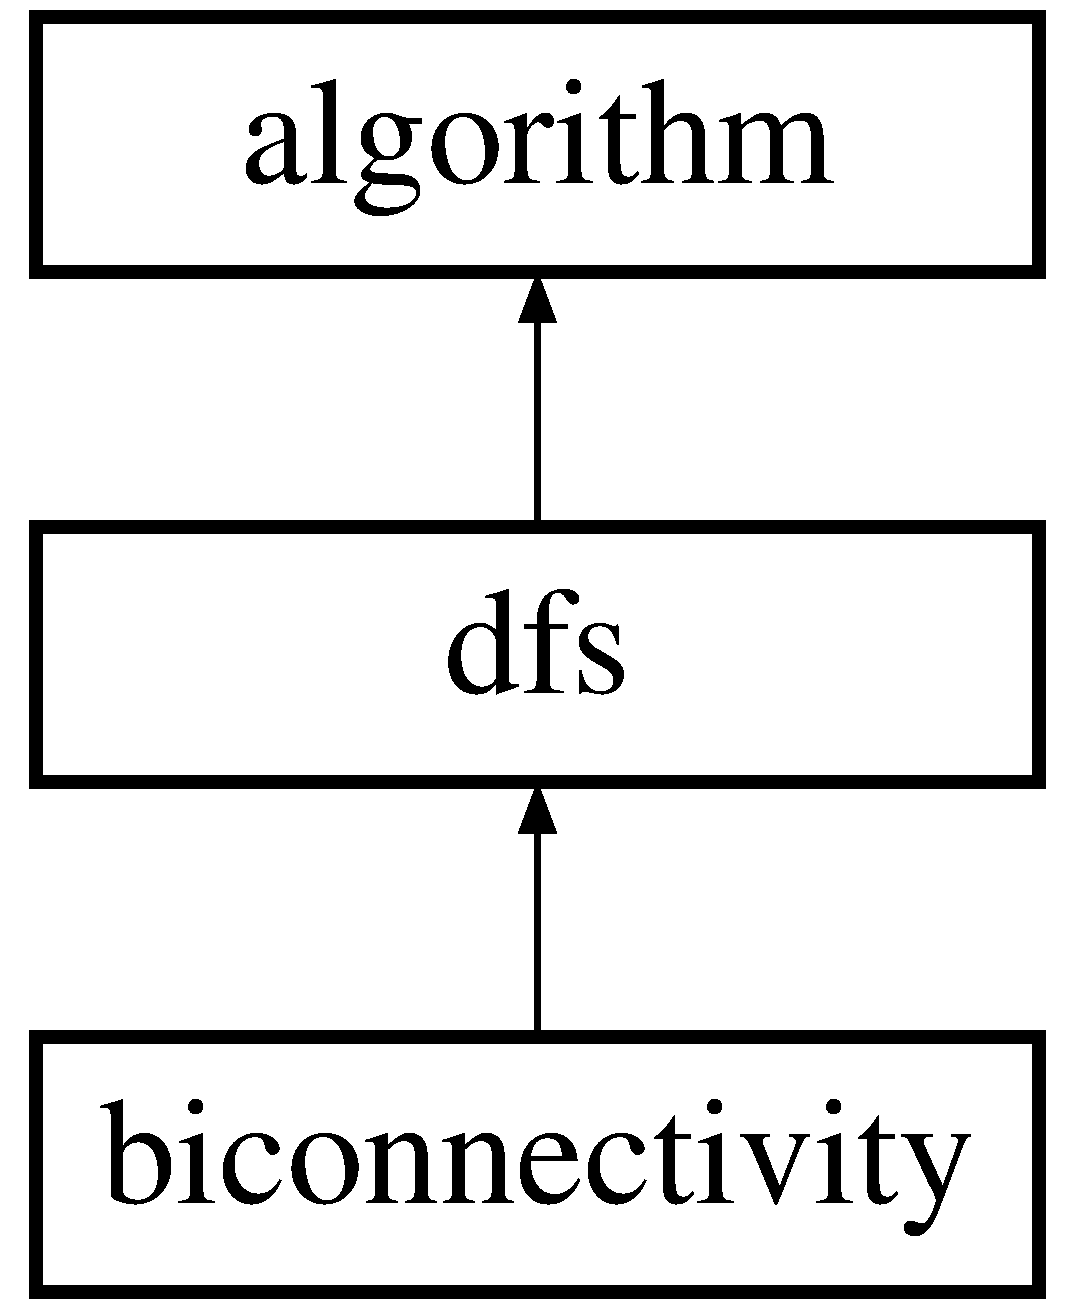
\includegraphics[height=3.000000cm]{classbiconnectivity}
\end{center}
\end{figure}
\subsection*{Public Types}
\begin{DoxyCompactItemize}
\item 
\mbox{\Hypertarget{classbiconnectivity_ad3823f78779cb1f2d4cf2117667f5ce7}\label{classbiconnectivity_ad3823f78779cb1f2d4cf2117667f5ce7}} 
typedef list$<$ \mbox{\hyperlink{classnode}{node}} $>$\+::iterator {\bfseries cutpoint\+\_\+iterator}
\item 
\mbox{\Hypertarget{classbiconnectivity_acf09990ddb220487655b4f57ccc5226f}\label{classbiconnectivity_acf09990ddb220487655b4f57ccc5226f}} 
typedef list$<$ pair$<$ list$<$ \mbox{\hyperlink{classnode}{node}} $>$, list$<$ \mbox{\hyperlink{classedge}{edge}} $>$ $>$ $>$\+::iterator {\bfseries component\+\_\+iterator}
\end{DoxyCompactItemize}
\subsection*{Public Member Functions}
\begin{DoxyCompactItemize}
\item 
\mbox{\hyperlink{classbiconnectivity_aec8c11afda486322b872f468cabd1f56}{biconnectivity}} ()
\begin{DoxyCompactList}\small\item\em Creates biconnectivity algorithm object. \end{DoxyCompactList}\item 
virtual \mbox{\hyperlink{classbiconnectivity_af8e2bb061de4a08f95a2a3a94fdbd797}{$\sim$biconnectivity}} ()
\begin{DoxyCompactList}\small\item\em Destroys biconnectivity algorithm object. \end{DoxyCompactList}\item 
virtual int \mbox{\hyperlink{classbiconnectivity_a65e0e821f5e9ce8d210648d462fd2cfa}{check}} (\mbox{\hyperlink{classgraph}{graph}} \&G)
\begin{DoxyCompactList}\small\item\em Checks whether the algorithm can be applied. \end{DoxyCompactList}\item 
virtual void \mbox{\hyperlink{classbiconnectivity_a4393dd1e626887472f6967722349abc6}{reset}} ()
\begin{DoxyCompactList}\small\item\em Resets algorithm. \end{DoxyCompactList}\item 
int \mbox{\hyperlink{classbiconnectivity_ab61a092bfc7cf9e9b27210d339186327}{low\+\_\+number}} (const \mbox{\hyperlink{classnode}{node}} \&n) const
\begin{DoxyCompactList}\small\item\em low-\/number. \end{DoxyCompactList}\item 
bool \mbox{\hyperlink{classbiconnectivity_a50e7cee997b6d56ccbb9ae3fd039d9cd}{is\+\_\+biconnected}} () const
\begin{DoxyCompactList}\small\item\em Biconnectivity-\/test. \end{DoxyCompactList}\item 
bool \mbox{\hyperlink{classbiconnectivity_a1234e7a70f50fd60c855529fe6fa4acb}{store\+\_\+components}} () const
\begin{DoxyCompactList}\small\item\em Returns whether the storing of components is enabled. \end{DoxyCompactList}\item 
void \mbox{\hyperlink{classbiconnectivity_ab7c9e256a4d7a4ffea33b20f014e1f69}{store\+\_\+components}} (bool set)
\begin{DoxyCompactList}\small\item\em Enables or disables the storing of biconnected components. \end{DoxyCompactList}\item 
void \mbox{\hyperlink{classbiconnectivity_a774fd08203a6d164605afc4cdc8b9201}{make\+\_\+biconnected}} (bool set)
\begin{DoxyCompactList}\small\item\em If enabled edges will be added to the graph in order to make it biconnected, if cutpoints are discovered. \end{DoxyCompactList}\item 
bool \mbox{\hyperlink{classbiconnectivity_a9ca9632a7fc398edb5b505dd0fe706c9}{make\+\_\+biconnected}} () const
\begin{DoxyCompactList}\small\item\em Returns whether addition of edges neccessary to make graph biconnected is enabled. \end{DoxyCompactList}\item 
list$<$ \mbox{\hyperlink{classedge}{edge}} $>$\+::iterator \mbox{\hyperlink{classbiconnectivity_ac5295da180114bffbbfd621d644d4c58}{additional\+\_\+begin}} ()
\begin{DoxyCompactList}\small\item\em Begin of edges added to make graph biconnected. \end{DoxyCompactList}\item 
list$<$ \mbox{\hyperlink{classedge}{edge}} $>$\+::iterator \mbox{\hyperlink{classbiconnectivity_a447a86f387efd181b25b8bacf3365e75}{additional\+\_\+end}} ()
\begin{DoxyCompactList}\small\item\em End of edges added to make graph biconnected. \end{DoxyCompactList}\item 
cutpoint\+\_\+iterator \mbox{\hyperlink{classbiconnectivity_a473197552874aaf148e847838144eed7}{cut\+\_\+points\+\_\+begin}} ()
\begin{DoxyCompactList}\small\item\em Start iteration over all cutpoints found. \end{DoxyCompactList}\item 
cutpoint\+\_\+iterator \mbox{\hyperlink{classbiconnectivity_a78cb06c1d056b9519622a67a92e85b6e}{cut\+\_\+points\+\_\+end}} ()
\begin{DoxyCompactList}\small\item\em End of iteration over all cutpoints. \end{DoxyCompactList}\item 
component\+\_\+iterator \mbox{\hyperlink{classbiconnectivity_ac0b7253533edc3f1412f771cb35bf04a}{components\+\_\+begin}} ()
\begin{DoxyCompactList}\small\item\em Start iteration over all biconnected components (if enabled during last call to run). \end{DoxyCompactList}\item 
component\+\_\+iterator \mbox{\hyperlink{classbiconnectivity_a0bd1c70975e664174e591efd64f8dc71}{components\+\_\+end}} ()
\begin{DoxyCompactList}\small\item\em End of iteration over all biconnected components. \end{DoxyCompactList}\item 
int \mbox{\hyperlink{classbiconnectivity_ad77634a59ac6a08fae43c1c38540d5f0}{number\+\_\+of\+\_\+components}} () const
\begin{DoxyCompactList}\small\item\em Number von biconnected components detected during the last run. \end{DoxyCompactList}\item 
virtual void \mbox{\hyperlink{classbiconnectivity_a64adab869e0080e3a1f8479e70010317}{init\+\_\+handler}} (\mbox{\hyperlink{classgraph}{graph}} \&)
\begin{DoxyCompactList}\small\item\em Handler called before the start of D\+FS. \end{DoxyCompactList}\item 
virtual void \mbox{\hyperlink{classbiconnectivity_acb402f2d144f84429b3cd009121245b0}{entry\+\_\+handler}} (\mbox{\hyperlink{classgraph}{graph}} \&, \mbox{\hyperlink{classnode}{node}} \&, \mbox{\hyperlink{classnode}{node}} \&)
\begin{DoxyCompactList}\small\item\em Handler called when touching node {\itshape n}. \end{DoxyCompactList}\item 
virtual void \mbox{\hyperlink{classbiconnectivity_a19261e91eef3f7d6b8586fa1eae9f277}{before\+\_\+recursive\+\_\+call\+\_\+handler}} (\mbox{\hyperlink{classgraph}{graph}} \&, \mbox{\hyperlink{classedge}{edge}} \&, \mbox{\hyperlink{classnode}{node}} \&)
\begin{DoxyCompactList}\small\item\em Handler called when a unused node {\itshape n} connected to the actual node by {\itshape e} is found. \end{DoxyCompactList}\item 
virtual void \mbox{\hyperlink{classbiconnectivity_a69ca91409485b57c486b188596080d7a}{after\+\_\+recursive\+\_\+call\+\_\+handler}} (\mbox{\hyperlink{classgraph}{graph}} \&, \mbox{\hyperlink{classedge}{edge}} \&, \mbox{\hyperlink{classnode}{node}} \&)
\begin{DoxyCompactList}\small\item\em Handler called after the algorithm returns from the subtree starting at {\itshape n} connected to the actual node by {\itshape e}. \end{DoxyCompactList}\item 
virtual void \mbox{\hyperlink{classbiconnectivity_a92228b87472140374dffea7d9f7ee20d}{old\+\_\+adj\+\_\+node\+\_\+handler}} (\mbox{\hyperlink{classgraph}{graph}} \&, \mbox{\hyperlink{classedge}{edge}} \&, \mbox{\hyperlink{classnode}{node}} \&)
\begin{DoxyCompactList}\small\item\em Handler called when a already marked node {\itshape n} connected to the actual node by {\itshape e} is found during the search of all adjacent edges of the actual node. \end{DoxyCompactList}\item 
virtual void \mbox{\hyperlink{classbiconnectivity_ae94213830755f1f4d477ec6bff0f25b8}{new\+\_\+start\+\_\+handler}} (\mbox{\hyperlink{classgraph}{graph}} \&, \mbox{\hyperlink{classnode}{node}} \&)
\begin{DoxyCompactList}\small\item\em Called when D\+FS is started with start-\/node {\itshape n}. \end{DoxyCompactList}\item 
virtual void \mbox{\hyperlink{classbiconnectivity_a868587fdc4dbb3bf80899d1c7d49b558}{leave\+\_\+handler}} (\mbox{\hyperlink{classgraph}{graph}} \&, \mbox{\hyperlink{classnode}{node}} \&, \mbox{\hyperlink{classnode}{node}} \&)
\begin{DoxyCompactList}\small\item\em Handler called after all the adjacent edges of {\itshape n} have been examined. \end{DoxyCompactList}\item 
virtual void \mbox{\hyperlink{classbiconnectivity_a2583331a4561f3db221ab674d2e5d75e}{end\+\_\+handler}} (\mbox{\hyperlink{classgraph}{graph}} \&)
\begin{DoxyCompactList}\small\item\em Handler called at the end of D\+FS. \end{DoxyCompactList}\end{DoxyCompactItemize}
\subsection*{Protected Attributes}
\begin{DoxyCompactItemize}
\item 
\mbox{\Hypertarget{classbiconnectivity_ab32b1a6264c24c6eec564cf082e980a1}\label{classbiconnectivity_ab32b1a6264c24c6eec564cf082e980a1}} 
list$<$ \mbox{\hyperlink{classedge}{edge}} $>$ {\bfseries self\+\_\+loops}
\item 
\mbox{\Hypertarget{classbiconnectivity_a487da69817fa89ab3d1523ad9846ae8e}\label{classbiconnectivity_a487da69817fa89ab3d1523ad9846ae8e}} 
\mbox{\hyperlink{classnode__map}{node\+\_\+map}}$<$ component\+\_\+iterator $>$ {\bfseries in\+\_\+component}
\item 
\mbox{\Hypertarget{classbiconnectivity_ac5817e2122477ed591ef229c081745f3}\label{classbiconnectivity_ac5817e2122477ed591ef229c081745f3}} 
\mbox{\hyperlink{classnode__map}{node\+\_\+map}}$<$ int $>$ {\bfseries low\+\_\+num}
\item 
\mbox{\Hypertarget{classbiconnectivity_a89fbd540b8a61aad150020be657ddfb7}\label{classbiconnectivity_a89fbd540b8a61aad150020be657ddfb7}} 
int {\bfseries num\+\_\+of\+\_\+components}
\item 
\mbox{\Hypertarget{classbiconnectivity_a989307b07f4a976649bd7551173bd564}\label{classbiconnectivity_a989307b07f4a976649bd7551173bd564}} 
bool {\bfseries store\+\_\+comp}
\item 
\mbox{\Hypertarget{classbiconnectivity_a70c1310b4ba83dbe10594f3a33f94763}\label{classbiconnectivity_a70c1310b4ba83dbe10594f3a33f94763}} 
bool {\bfseries add\+\_\+edges}
\item 
\mbox{\Hypertarget{classbiconnectivity_a6f2e474efeb8ccb023d9b84385798193}\label{classbiconnectivity_a6f2e474efeb8ccb023d9b84385798193}} 
\mbox{\hyperlink{classnode}{node}} {\bfseries last}
\item 
\mbox{\Hypertarget{classbiconnectivity_a6b33fabd4da60c573adfb0538f28e0ed}\label{classbiconnectivity_a6b33fabd4da60c573adfb0538f28e0ed}} 
stack$<$ \mbox{\hyperlink{classnode}{node}} $>$ {\bfseries node\+\_\+stack}
\item 
\mbox{\Hypertarget{classbiconnectivity_aaf715d6044028c456515389e879dd5d8}\label{classbiconnectivity_aaf715d6044028c456515389e879dd5d8}} 
stack$<$ \mbox{\hyperlink{classedge}{edge}} $>$ {\bfseries edge\+\_\+stack}
\item 
\mbox{\Hypertarget{classbiconnectivity_a1d484917f1822478d148647cfae05605}\label{classbiconnectivity_a1d484917f1822478d148647cfae05605}} 
list$<$ pair$<$ list$<$ \mbox{\hyperlink{classnode}{node}} $>$, list$<$ \mbox{\hyperlink{classedge}{edge}} $>$ $>$ $>$ {\bfseries components}
\item 
\mbox{\Hypertarget{classbiconnectivity_a1591f1872a681e0dce0066ea00763c67}\label{classbiconnectivity_a1591f1872a681e0dce0066ea00763c67}} 
list$<$ \mbox{\hyperlink{classnode}{node}} $>$ {\bfseries cut\+\_\+points}
\item 
\mbox{\Hypertarget{classbiconnectivity_a67756de28954d13df615d8f2a93b22da}\label{classbiconnectivity_a67756de28954d13df615d8f2a93b22da}} 
\mbox{\hyperlink{classnode__map}{node\+\_\+map}}$<$ int $>$ {\bfseries cut\+\_\+count}
\item 
\mbox{\Hypertarget{classbiconnectivity_a14148f2d705d6ed29f1b2370104a41b1}\label{classbiconnectivity_a14148f2d705d6ed29f1b2370104a41b1}} 
list$<$ \mbox{\hyperlink{classedge}{edge}} $>$ {\bfseries additional}
\item 
\mbox{\Hypertarget{classbiconnectivity_a3292c5b6bf3b91947509a380cf779706}\label{classbiconnectivity_a3292c5b6bf3b91947509a380cf779706}} 
\mbox{\hyperlink{classnode__map}{node\+\_\+map}}$<$ \mbox{\hyperlink{classnode}{node}} $>$ {\bfseries first\+\_\+child}
\end{DoxyCompactItemize}


\subsection{Detailed Description}
Biconnectivity-\/test and low-\/numbers. 

\begin{DoxyParagraph}{Date}
2019/05/07 13\+:37\+:14 
\end{DoxyParagraph}
\begin{DoxyParagraph}{Revision}
1.\+18 
\end{DoxyParagraph}


Obviously there is a close relationship between D\+FS and the testing of biconnectivity. Thus this test takes advantage of the possibility to add pieces of code to the D\+F\+S-\/class in order to calculate the low-\/numbers.

As default no biconnected components will be stored and no edges will be added to make the graph biconnected. The test will run on the whole graph, even if it is not connected. 

\subsection{Constructor \& Destructor Documentation}
\mbox{\Hypertarget{classbiconnectivity_aec8c11afda486322b872f468cabd1f56}\label{classbiconnectivity_aec8c11afda486322b872f468cabd1f56}} 
\index{biconnectivity@{biconnectivity}!biconnectivity@{biconnectivity}}
\index{biconnectivity@{biconnectivity}!biconnectivity@{biconnectivity}}
\subsubsection{\texorpdfstring{biconnectivity()}{biconnectivity()}}
{\footnotesize\ttfamily \+\_\+\+\_\+\+K\+G\+L\+\_\+\+B\+E\+G\+I\+N\+\_\+\+N\+A\+M\+E\+S\+P\+A\+CE biconnectivity\+::biconnectivity (\begin{DoxyParamCaption}{ }\end{DoxyParamCaption})}



Creates biconnectivity algorithm object. 

\begin{DoxySeeAlso}{See also}
\mbox{\hyperlink{classdfs_a5232bc41ab202b6278a84bd97c803a0d}{dfs\+::dfs}} 
\end{DoxySeeAlso}
\mbox{\Hypertarget{classbiconnectivity_af8e2bb061de4a08f95a2a3a94fdbd797}\label{classbiconnectivity_af8e2bb061de4a08f95a2a3a94fdbd797}} 
\index{biconnectivity@{biconnectivity}!````~biconnectivity@{$\sim$biconnectivity}}
\index{````~biconnectivity@{$\sim$biconnectivity}!biconnectivity@{biconnectivity}}
\subsubsection{\texorpdfstring{$\sim$biconnectivity()}{~biconnectivity()}}
{\footnotesize\ttfamily virtual biconnectivity\+::$\sim$biconnectivity (\begin{DoxyParamCaption}{ }\end{DoxyParamCaption})\hspace{0.3cm}{\ttfamily [inline]}, {\ttfamily [virtual]}}



Destroys biconnectivity algorithm object. 

\begin{DoxySeeAlso}{See also}
\mbox{\hyperlink{classdfs_aff2e95c12935221a94551393f7e36c6e}{dfs\+::$\sim$dfs}} 
\end{DoxySeeAlso}


\subsection{Member Function Documentation}
\mbox{\Hypertarget{classbiconnectivity_ac5295da180114bffbbfd621d644d4c58}\label{classbiconnectivity_ac5295da180114bffbbfd621d644d4c58}} 
\index{biconnectivity@{biconnectivity}!additional\+\_\+begin@{additional\+\_\+begin}}
\index{additional\+\_\+begin@{additional\+\_\+begin}!biconnectivity@{biconnectivity}}
\subsubsection{\texorpdfstring{additional\+\_\+begin()}{additional\_begin()}}
{\footnotesize\ttfamily list$<$\mbox{\hyperlink{classedge}{edge}}$>$\+::iterator biconnectivity\+::additional\+\_\+begin (\begin{DoxyParamCaption}{ }\end{DoxyParamCaption})\hspace{0.3cm}{\ttfamily [inline]}}



Begin of edges added to make graph biconnected. 

\begin{DoxyReturn}{Returns}
begin of additional edges 
\end{DoxyReturn}
\begin{DoxySeeAlso}{See also}
\mbox{\hyperlink{classbiconnectivity_a774fd08203a6d164605afc4cdc8b9201}{biconnectivity\+::make\+\_\+biconnected}} 
\end{DoxySeeAlso}
\mbox{\Hypertarget{classbiconnectivity_a447a86f387efd181b25b8bacf3365e75}\label{classbiconnectivity_a447a86f387efd181b25b8bacf3365e75}} 
\index{biconnectivity@{biconnectivity}!additional\+\_\+end@{additional\+\_\+end}}
\index{additional\+\_\+end@{additional\+\_\+end}!biconnectivity@{biconnectivity}}
\subsubsection{\texorpdfstring{additional\+\_\+end()}{additional\_end()}}
{\footnotesize\ttfamily list$<$\mbox{\hyperlink{classedge}{edge}}$>$\+::iterator biconnectivity\+::additional\+\_\+end (\begin{DoxyParamCaption}{ }\end{DoxyParamCaption})\hspace{0.3cm}{\ttfamily [inline]}}



End of edges added to make graph biconnected. 

\begin{DoxyReturn}{Returns}
end of additional edges 
\end{DoxyReturn}
\begin{DoxySeeAlso}{See also}
\mbox{\hyperlink{classbiconnectivity_a774fd08203a6d164605afc4cdc8b9201}{biconnectivity\+::make\+\_\+biconnected}} 
\end{DoxySeeAlso}
\mbox{\Hypertarget{classbiconnectivity_a69ca91409485b57c486b188596080d7a}\label{classbiconnectivity_a69ca91409485b57c486b188596080d7a}} 
\index{biconnectivity@{biconnectivity}!after\+\_\+recursive\+\_\+call\+\_\+handler@{after\+\_\+recursive\+\_\+call\+\_\+handler}}
\index{after\+\_\+recursive\+\_\+call\+\_\+handler@{after\+\_\+recursive\+\_\+call\+\_\+handler}!biconnectivity@{biconnectivity}}
\subsubsection{\texorpdfstring{after\+\_\+recursive\+\_\+call\+\_\+handler()}{after\_recursive\_call\_handler()}}
{\footnotesize\ttfamily void biconnectivity\+::after\+\_\+recursive\+\_\+call\+\_\+handler (\begin{DoxyParamCaption}\item[{\mbox{\hyperlink{classgraph}{graph}} \&}]{G,  }\item[{\mbox{\hyperlink{classedge}{edge}} \&}]{e,  }\item[{\mbox{\hyperlink{classnode}{node}} \&}]{n }\end{DoxyParamCaption})\hspace{0.3cm}{\ttfamily [virtual]}}



Handler called after the algorithm returns from the subtree starting at {\itshape n} connected to the actual node by {\itshape e}. 


\begin{DoxyParams}{Parameters}
{\em G} & graph for which D\+FS was invoked. \\
\hline
{\em e} & edge connecting the actual node to the unused one. \\
\hline
{\em n} & unused node. \\
\hline
\end{DoxyParams}


Reimplemented from \mbox{\hyperlink{classdfs_a25ae75fe08f1d8c0fedcf9dcae09d092}{dfs}}.

\mbox{\Hypertarget{classbiconnectivity_a19261e91eef3f7d6b8586fa1eae9f277}\label{classbiconnectivity_a19261e91eef3f7d6b8586fa1eae9f277}} 
\index{biconnectivity@{biconnectivity}!before\+\_\+recursive\+\_\+call\+\_\+handler@{before\+\_\+recursive\+\_\+call\+\_\+handler}}
\index{before\+\_\+recursive\+\_\+call\+\_\+handler@{before\+\_\+recursive\+\_\+call\+\_\+handler}!biconnectivity@{biconnectivity}}
\subsubsection{\texorpdfstring{before\+\_\+recursive\+\_\+call\+\_\+handler()}{before\_recursive\_call\_handler()}}
{\footnotesize\ttfamily void biconnectivity\+::before\+\_\+recursive\+\_\+call\+\_\+handler (\begin{DoxyParamCaption}\item[{\mbox{\hyperlink{classgraph}{graph}} \&}]{G,  }\item[{\mbox{\hyperlink{classedge}{edge}} \&}]{e,  }\item[{\mbox{\hyperlink{classnode}{node}} \&}]{n }\end{DoxyParamCaption})\hspace{0.3cm}{\ttfamily [virtual]}}



Handler called when a unused node {\itshape n} connected to the actual node by {\itshape e} is found. 


\begin{DoxyParams}{Parameters}
{\em G} & graph for which D\+FS was invoked. \\
\hline
{\em e} & edge connecting the actual node to the unused one. \\
\hline
{\em n} & unused node. \\
\hline
\end{DoxyParams}


Reimplemented from \mbox{\hyperlink{classdfs_ae3f095c9fe6106e82c24543da4844ea3}{dfs}}.

\mbox{\Hypertarget{classbiconnectivity_a65e0e821f5e9ce8d210648d462fd2cfa}\label{classbiconnectivity_a65e0e821f5e9ce8d210648d462fd2cfa}} 
\index{biconnectivity@{biconnectivity}!check@{check}}
\index{check@{check}!biconnectivity@{biconnectivity}}
\subsubsection{\texorpdfstring{check()}{check()}}
{\footnotesize\ttfamily int biconnectivity\+::check (\begin{DoxyParamCaption}\item[{\mbox{\hyperlink{classgraph}{graph}} \&}]{G }\end{DoxyParamCaption})\hspace{0.3cm}{\ttfamily [virtual]}}



Checks whether the algorithm can be applied. 

Necessary preconditions\+:
\begin{DoxyItemize}
\item G is undirected.
\item storing of predecessors is enabled.
\item D\+FS may be applied
\end{DoxyItemize}


\begin{DoxyParams}{Parameters}
{\em G} & graph. \\
\hline
\end{DoxyParams}
\begin{DoxyReturn}{Returns}
\mbox{\hyperlink{classalgorithm_af1a0078e153aa99c24f9bdf0d97f6710aae4c1cd7fe8d8cf4b143241a6e7c31cf}{algorithm\+::\+K\+G\+L\+\_\+\+OK}} if binconnectivity-\/test can be applied to {\itshape G}. 
\end{DoxyReturn}
\begin{DoxySeeAlso}{See also}
\mbox{\hyperlink{classdfs_aa7c864a6f3a120720138b187b3ed95b5}{dfs\+::scan\+\_\+whole\+\_\+graph}}, \mbox{\hyperlink{classdfs_a7043f46eb3887cbcbb1391fc783407a4}{dfs\+::store\+\_\+preds}} 
\end{DoxySeeAlso}


Reimplemented from \mbox{\hyperlink{classdfs_a1af70060897529e67910f589b047e576}{dfs}}.

\mbox{\Hypertarget{classbiconnectivity_ac0b7253533edc3f1412f771cb35bf04a}\label{classbiconnectivity_ac0b7253533edc3f1412f771cb35bf04a}} 
\index{biconnectivity@{biconnectivity}!components\+\_\+begin@{components\+\_\+begin}}
\index{components\+\_\+begin@{components\+\_\+begin}!biconnectivity@{biconnectivity}}
\subsubsection{\texorpdfstring{components\+\_\+begin()}{components\_begin()}}
{\footnotesize\ttfamily component\+\_\+iterator biconnectivity\+::components\+\_\+begin (\begin{DoxyParamCaption}{ }\end{DoxyParamCaption})\hspace{0.3cm}{\ttfamily [inline]}}



Start iteration over all biconnected components (if enabled during last call to run). 

Components are represented as a pair consisting of a list of nodes and a list of edges, i.\+e. if it is of type component\+\_\+iterator then $\ast$it is of type pair$<$list$<$node$>$,list$<$edge$>$ $>$.

\begin{DoxyReturn}{Returns}
iterator to first component 
\end{DoxyReturn}
\begin{DoxySeeAlso}{See also}
\mbox{\hyperlink{classbiconnectivity_a1234e7a70f50fd60c855529fe6fa4acb}{biconnectivity\+::store\+\_\+components}} 
\end{DoxySeeAlso}
\mbox{\Hypertarget{classbiconnectivity_a0bd1c70975e664174e591efd64f8dc71}\label{classbiconnectivity_a0bd1c70975e664174e591efd64f8dc71}} 
\index{biconnectivity@{biconnectivity}!components\+\_\+end@{components\+\_\+end}}
\index{components\+\_\+end@{components\+\_\+end}!biconnectivity@{biconnectivity}}
\subsubsection{\texorpdfstring{components\+\_\+end()}{components\_end()}}
{\footnotesize\ttfamily component\+\_\+iterator biconnectivity\+::components\+\_\+end (\begin{DoxyParamCaption}{ }\end{DoxyParamCaption})\hspace{0.3cm}{\ttfamily [inline]}}



End of iteration over all biconnected components. 

\begin{DoxyReturn}{Returns}
end of iteration over biconnected components 
\end{DoxyReturn}
\begin{DoxySeeAlso}{See also}
\mbox{\hyperlink{classbiconnectivity_a1234e7a70f50fd60c855529fe6fa4acb}{biconnectivity\+::store\+\_\+components}} 
\end{DoxySeeAlso}
\mbox{\Hypertarget{classbiconnectivity_a473197552874aaf148e847838144eed7}\label{classbiconnectivity_a473197552874aaf148e847838144eed7}} 
\index{biconnectivity@{biconnectivity}!cut\+\_\+points\+\_\+begin@{cut\+\_\+points\+\_\+begin}}
\index{cut\+\_\+points\+\_\+begin@{cut\+\_\+points\+\_\+begin}!biconnectivity@{biconnectivity}}
\subsubsection{\texorpdfstring{cut\+\_\+points\+\_\+begin()}{cut\_points\_begin()}}
{\footnotesize\ttfamily cutpoint\+\_\+iterator biconnectivity\+::cut\+\_\+points\+\_\+begin (\begin{DoxyParamCaption}{ }\end{DoxyParamCaption})\hspace{0.3cm}{\ttfamily [inline]}}



Start iteration over all cutpoints found. 

A cutpoints is a node whose removal will disconnect the graph, thus a graph with no cutpoints is biconnected and vice versa.

\begin{DoxyReturn}{Returns}
iterator to first cutpoint. 
\end{DoxyReturn}
\begin{DoxySeeAlso}{See also}
\mbox{\hyperlink{classbiconnectivity_a78cb06c1d056b9519622a67a92e85b6e}{biconnectivity\+::cut\+\_\+points\+\_\+end}} 
\end{DoxySeeAlso}
\mbox{\Hypertarget{classbiconnectivity_a78cb06c1d056b9519622a67a92e85b6e}\label{classbiconnectivity_a78cb06c1d056b9519622a67a92e85b6e}} 
\index{biconnectivity@{biconnectivity}!cut\+\_\+points\+\_\+end@{cut\+\_\+points\+\_\+end}}
\index{cut\+\_\+points\+\_\+end@{cut\+\_\+points\+\_\+end}!biconnectivity@{biconnectivity}}
\subsubsection{\texorpdfstring{cut\+\_\+points\+\_\+end()}{cut\_points\_end()}}
{\footnotesize\ttfamily cutpoint\+\_\+iterator biconnectivity\+::cut\+\_\+points\+\_\+end (\begin{DoxyParamCaption}{ }\end{DoxyParamCaption})\hspace{0.3cm}{\ttfamily [inline]}}



End of iteration over all cutpoints. 

\begin{DoxyReturn}{Returns}
one-\/past-\/the-\/end iterator. 
\end{DoxyReturn}
\begin{DoxySeeAlso}{See also}
\mbox{\hyperlink{classbiconnectivity_a473197552874aaf148e847838144eed7}{biconnectivity\+::cut\+\_\+points\+\_\+begin}} 
\end{DoxySeeAlso}
\mbox{\Hypertarget{classbiconnectivity_a2583331a4561f3db221ab674d2e5d75e}\label{classbiconnectivity_a2583331a4561f3db221ab674d2e5d75e}} 
\index{biconnectivity@{biconnectivity}!end\+\_\+handler@{end\+\_\+handler}}
\index{end\+\_\+handler@{end\+\_\+handler}!biconnectivity@{biconnectivity}}
\subsubsection{\texorpdfstring{end\+\_\+handler()}{end\_handler()}}
{\footnotesize\ttfamily void biconnectivity\+::end\+\_\+handler (\begin{DoxyParamCaption}\item[{\mbox{\hyperlink{classgraph}{graph}} \&}]{G }\end{DoxyParamCaption})\hspace{0.3cm}{\ttfamily [virtual]}}



Handler called at the end of D\+FS. 


\begin{DoxyParams}{Parameters}
{\em G} & graph for which D\+FS was invoked. \\
\hline
\end{DoxyParams}


Reimplemented from \mbox{\hyperlink{classdfs_ab96c7c6183856dd9e356fdcf50835b32}{dfs}}.

\mbox{\Hypertarget{classbiconnectivity_acb402f2d144f84429b3cd009121245b0}\label{classbiconnectivity_acb402f2d144f84429b3cd009121245b0}} 
\index{biconnectivity@{biconnectivity}!entry\+\_\+handler@{entry\+\_\+handler}}
\index{entry\+\_\+handler@{entry\+\_\+handler}!biconnectivity@{biconnectivity}}
\subsubsection{\texorpdfstring{entry\+\_\+handler()}{entry\_handler()}}
{\footnotesize\ttfamily void biconnectivity\+::entry\+\_\+handler (\begin{DoxyParamCaption}\item[{\mbox{\hyperlink{classgraph}{graph}} \&}]{G,  }\item[{\mbox{\hyperlink{classnode}{node}} \&}]{n,  }\item[{\mbox{\hyperlink{classnode}{node}} \&}]{f }\end{DoxyParamCaption})\hspace{0.3cm}{\ttfamily [virtual]}}



Handler called when touching node {\itshape n}. 


\begin{DoxyParams}{Parameters}
{\em G} & graph for which D\+FS was invoked. \\
\hline
{\em n} & actual node. \\
\hline
{\em f} & predecessor. \\
\hline
\end{DoxyParams}


Reimplemented from \mbox{\hyperlink{classdfs_a73dabe5882226b53494a487b7c34f1d1}{dfs}}.

\mbox{\Hypertarget{classbiconnectivity_a64adab869e0080e3a1f8479e70010317}\label{classbiconnectivity_a64adab869e0080e3a1f8479e70010317}} 
\index{biconnectivity@{biconnectivity}!init\+\_\+handler@{init\+\_\+handler}}
\index{init\+\_\+handler@{init\+\_\+handler}!biconnectivity@{biconnectivity}}
\subsubsection{\texorpdfstring{init\+\_\+handler()}{init\_handler()}}
{\footnotesize\ttfamily void biconnectivity\+::init\+\_\+handler (\begin{DoxyParamCaption}\item[{\mbox{\hyperlink{classgraph}{graph}} \&}]{G }\end{DoxyParamCaption})\hspace{0.3cm}{\ttfamily [virtual]}}



Handler called before the start of D\+FS. 


\begin{DoxyParams}{Parameters}
{\em G} & graph for which D\+FS was invoked. \\
\hline
\end{DoxyParams}


Reimplemented from \mbox{\hyperlink{classdfs_acc82574cd42ab8256e685374bee5fabb}{dfs}}.

\mbox{\Hypertarget{classbiconnectivity_a50e7cee997b6d56ccbb9ae3fd039d9cd}\label{classbiconnectivity_a50e7cee997b6d56ccbb9ae3fd039d9cd}} 
\index{biconnectivity@{biconnectivity}!is\+\_\+biconnected@{is\+\_\+biconnected}}
\index{is\+\_\+biconnected@{is\+\_\+biconnected}!biconnectivity@{biconnectivity}}
\subsubsection{\texorpdfstring{is\+\_\+biconnected()}{is\_biconnected()}}
{\footnotesize\ttfamily bool biconnectivity\+::is\+\_\+biconnected (\begin{DoxyParamCaption}{ }\end{DoxyParamCaption}) const\hspace{0.3cm}{\ttfamily [inline]}}



Biconnectivity-\/test. 

\begin{DoxyReturn}{Returns}
true iff graph is biconnected. 
\end{DoxyReturn}
\mbox{\Hypertarget{classbiconnectivity_a868587fdc4dbb3bf80899d1c7d49b558}\label{classbiconnectivity_a868587fdc4dbb3bf80899d1c7d49b558}} 
\index{biconnectivity@{biconnectivity}!leave\+\_\+handler@{leave\+\_\+handler}}
\index{leave\+\_\+handler@{leave\+\_\+handler}!biconnectivity@{biconnectivity}}
\subsubsection{\texorpdfstring{leave\+\_\+handler()}{leave\_handler()}}
{\footnotesize\ttfamily void biconnectivity\+::leave\+\_\+handler (\begin{DoxyParamCaption}\item[{\mbox{\hyperlink{classgraph}{graph}} \&}]{G,  }\item[{\mbox{\hyperlink{classnode}{node}} \&}]{n,  }\item[{\mbox{\hyperlink{classnode}{node}} \&}]{f }\end{DoxyParamCaption})\hspace{0.3cm}{\ttfamily [virtual]}}



Handler called after all the adjacent edges of {\itshape n} have been examined. 


\begin{DoxyParams}{Parameters}
{\em G} & graph for which D\+FS was invoked. \\
\hline
{\em n} & actual node. \\
\hline
{\em f} & predecessor. \\
\hline
\end{DoxyParams}


Reimplemented from \mbox{\hyperlink{classdfs_a8071fc4e82deff7ceb2790cd4eb42280}{dfs}}.

\mbox{\Hypertarget{classbiconnectivity_ab61a092bfc7cf9e9b27210d339186327}\label{classbiconnectivity_ab61a092bfc7cf9e9b27210d339186327}} 
\index{biconnectivity@{biconnectivity}!low\+\_\+number@{low\+\_\+number}}
\index{low\+\_\+number@{low\+\_\+number}!biconnectivity@{biconnectivity}}
\subsubsection{\texorpdfstring{low\+\_\+number()}{low\_number()}}
{\footnotesize\ttfamily int biconnectivity\+::low\+\_\+number (\begin{DoxyParamCaption}\item[{const \mbox{\hyperlink{classnode}{node}} \&}]{n }\end{DoxyParamCaption}) const\hspace{0.3cm}{\ttfamily [inline]}}



low-\/number. 


\begin{DoxyParams}{Parameters}
{\em n} & node. \\
\hline
\end{DoxyParams}
\begin{DoxyReturn}{Returns}
low-\/number of n. 
\end{DoxyReturn}
\mbox{\Hypertarget{classbiconnectivity_a774fd08203a6d164605afc4cdc8b9201}\label{classbiconnectivity_a774fd08203a6d164605afc4cdc8b9201}} 
\index{biconnectivity@{biconnectivity}!make\+\_\+biconnected@{make\+\_\+biconnected}}
\index{make\+\_\+biconnected@{make\+\_\+biconnected}!biconnectivity@{biconnectivity}}
\subsubsection{\texorpdfstring{make\+\_\+biconnected()}{make\_biconnected()}\hspace{0.1cm}{\footnotesize\ttfamily [1/2]}}
{\footnotesize\ttfamily void biconnectivity\+::make\+\_\+biconnected (\begin{DoxyParamCaption}\item[{bool}]{set }\end{DoxyParamCaption})\hspace{0.3cm}{\ttfamily [inline]}}



If enabled edges will be added to the graph in order to make it biconnected, if cutpoints are discovered. 

The list of added edges can be accessed via additional\+\_\+begin and additional\+\_\+end.


\begin{DoxyParams}{Parameters}
{\em set} & if true additional edges will we inserted to make the graph biconnected. \\
\hline
\end{DoxyParams}
\begin{DoxySeeAlso}{See also}
\mbox{\hyperlink{classbiconnectivity_ac5295da180114bffbbfd621d644d4c58}{biconnectivity\+::additional\+\_\+begin}}, \mbox{\hyperlink{classbiconnectivity_a447a86f387efd181b25b8bacf3365e75}{biconnectivity\+::additional\+\_\+end}} 
\end{DoxySeeAlso}
\mbox{\Hypertarget{classbiconnectivity_a9ca9632a7fc398edb5b505dd0fe706c9}\label{classbiconnectivity_a9ca9632a7fc398edb5b505dd0fe706c9}} 
\index{biconnectivity@{biconnectivity}!make\+\_\+biconnected@{make\+\_\+biconnected}}
\index{make\+\_\+biconnected@{make\+\_\+biconnected}!biconnectivity@{biconnectivity}}
\subsubsection{\texorpdfstring{make\+\_\+biconnected()}{make\_biconnected()}\hspace{0.1cm}{\footnotesize\ttfamily [2/2]}}
{\footnotesize\ttfamily bool biconnectivity\+::make\+\_\+biconnected (\begin{DoxyParamCaption}{ }\end{DoxyParamCaption}) const\hspace{0.3cm}{\ttfamily [inline]}}



Returns whether addition of edges neccessary to make graph biconnected is enabled. 

\begin{DoxyReturn}{Returns}
true iff addition edges is enabled. 
\end{DoxyReturn}
\begin{DoxySeeAlso}{See also}
\mbox{\hyperlink{classbiconnectivity_ac5295da180114bffbbfd621d644d4c58}{biconnectivity\+::additional\+\_\+begin}}, \mbox{\hyperlink{classbiconnectivity_a447a86f387efd181b25b8bacf3365e75}{biconnectivity\+::additional\+\_\+end}} 
\end{DoxySeeAlso}
\mbox{\Hypertarget{classbiconnectivity_ae94213830755f1f4d477ec6bff0f25b8}\label{classbiconnectivity_ae94213830755f1f4d477ec6bff0f25b8}} 
\index{biconnectivity@{biconnectivity}!new\+\_\+start\+\_\+handler@{new\+\_\+start\+\_\+handler}}
\index{new\+\_\+start\+\_\+handler@{new\+\_\+start\+\_\+handler}!biconnectivity@{biconnectivity}}
\subsubsection{\texorpdfstring{new\+\_\+start\+\_\+handler()}{new\_start\_handler()}}
{\footnotesize\ttfamily void biconnectivity\+::new\+\_\+start\+\_\+handler (\begin{DoxyParamCaption}\item[{\mbox{\hyperlink{classgraph}{graph}} \&}]{G,  }\item[{\mbox{\hyperlink{classnode}{node}} \&}]{n }\end{DoxyParamCaption})\hspace{0.3cm}{\ttfamily [virtual]}}



Called when D\+FS is started with start-\/node {\itshape n}. 

This is particularly useful when D\+FS was invoked with the \mbox{\hyperlink{classdfs_aa7c864a6f3a120720138b187b3ed95b5}{scan\+\_\+whole\+\_\+graph}} option.


\begin{DoxyParams}{Parameters}
{\em G} & graph for which D\+FS was invoked. \\
\hline
{\em n} & start-\/node. \\
\hline
\end{DoxyParams}


Reimplemented from \mbox{\hyperlink{classdfs_a3b5fbea7a7baed9946cfb4444a7f20ea}{dfs}}.

\mbox{\Hypertarget{classbiconnectivity_ad77634a59ac6a08fae43c1c38540d5f0}\label{classbiconnectivity_ad77634a59ac6a08fae43c1c38540d5f0}} 
\index{biconnectivity@{biconnectivity}!number\+\_\+of\+\_\+components@{number\+\_\+of\+\_\+components}}
\index{number\+\_\+of\+\_\+components@{number\+\_\+of\+\_\+components}!biconnectivity@{biconnectivity}}
\subsubsection{\texorpdfstring{number\+\_\+of\+\_\+components()}{number\_of\_components()}}
{\footnotesize\ttfamily int biconnectivity\+::number\+\_\+of\+\_\+components (\begin{DoxyParamCaption}{ }\end{DoxyParamCaption}) const\hspace{0.3cm}{\ttfamily [inline]}}



Number von biconnected components detected during the last run. 

\begin{DoxyReturn}{Returns}
number of biconnected components. 
\end{DoxyReturn}
\mbox{\Hypertarget{classbiconnectivity_a92228b87472140374dffea7d9f7ee20d}\label{classbiconnectivity_a92228b87472140374dffea7d9f7ee20d}} 
\index{biconnectivity@{biconnectivity}!old\+\_\+adj\+\_\+node\+\_\+handler@{old\+\_\+adj\+\_\+node\+\_\+handler}}
\index{old\+\_\+adj\+\_\+node\+\_\+handler@{old\+\_\+adj\+\_\+node\+\_\+handler}!biconnectivity@{biconnectivity}}
\subsubsection{\texorpdfstring{old\+\_\+adj\+\_\+node\+\_\+handler()}{old\_adj\_node\_handler()}}
{\footnotesize\ttfamily void biconnectivity\+::old\+\_\+adj\+\_\+node\+\_\+handler (\begin{DoxyParamCaption}\item[{\mbox{\hyperlink{classgraph}{graph}} \&}]{G,  }\item[{\mbox{\hyperlink{classedge}{edge}} \&}]{e,  }\item[{\mbox{\hyperlink{classnode}{node}} \&}]{n }\end{DoxyParamCaption})\hspace{0.3cm}{\ttfamily [virtual]}}



Handler called when a already marked node {\itshape n} connected to the actual node by {\itshape e} is found during the search of all adjacent edges of the actual node. 


\begin{DoxyParams}{Parameters}
{\em G} & graph for which D\+FS was invoked. \\
\hline
{\em e} & edge connecting the actual node to the old one. \\
\hline
{\em n} & used node. \\
\hline
\end{DoxyParams}


Reimplemented from \mbox{\hyperlink{classdfs_adf1c667188e632761c63f529537c544c}{dfs}}.

\mbox{\Hypertarget{classbiconnectivity_a4393dd1e626887472f6967722349abc6}\label{classbiconnectivity_a4393dd1e626887472f6967722349abc6}} 
\index{biconnectivity@{biconnectivity}!reset@{reset}}
\index{reset@{reset}!biconnectivity@{biconnectivity}}
\subsubsection{\texorpdfstring{reset()}{reset()}}
{\footnotesize\ttfamily void biconnectivity\+::reset (\begin{DoxyParamCaption}{ }\end{DoxyParamCaption})\hspace{0.3cm}{\ttfamily [virtual]}}



Resets algorithm. 

Prepares the algorithm to be applied to another graph. {\itshape Please} {\itshape note\+:} The options an algorithm may support do {\itshape not} get reset by this. It is just to reset internally used datastructures. 

Reimplemented from \mbox{\hyperlink{classdfs_affaffda8be8418d6dbf396c5b1d6b81a}{dfs}}.

\mbox{\Hypertarget{classbiconnectivity_a1234e7a70f50fd60c855529fe6fa4acb}\label{classbiconnectivity_a1234e7a70f50fd60c855529fe6fa4acb}} 
\index{biconnectivity@{biconnectivity}!store\+\_\+components@{store\+\_\+components}}
\index{store\+\_\+components@{store\+\_\+components}!biconnectivity@{biconnectivity}}
\subsubsection{\texorpdfstring{store\+\_\+components()}{store\_components()}\hspace{0.1cm}{\footnotesize\ttfamily [1/2]}}
{\footnotesize\ttfamily bool biconnectivity\+::store\+\_\+components (\begin{DoxyParamCaption}{ }\end{DoxyParamCaption}) const\hspace{0.3cm}{\ttfamily [inline]}}



Returns whether the storing of components is enabled. 

\begin{DoxyReturn}{Returns}
true iff storing of components is enabled. 
\end{DoxyReturn}
\begin{DoxySeeAlso}{See also}
\mbox{\hyperlink{classbiconnectivity_ac0b7253533edc3f1412f771cb35bf04a}{biconnectivity\+::components\+\_\+begin}}, \mbox{\hyperlink{classbiconnectivity_a0bd1c70975e664174e591efd64f8dc71}{biconnectivity\+::components\+\_\+end}} 
\end{DoxySeeAlso}
\mbox{\Hypertarget{classbiconnectivity_ab7c9e256a4d7a4ffea33b20f014e1f69}\label{classbiconnectivity_ab7c9e256a4d7a4ffea33b20f014e1f69}} 
\index{biconnectivity@{biconnectivity}!store\+\_\+components@{store\+\_\+components}}
\index{store\+\_\+components@{store\+\_\+components}!biconnectivity@{biconnectivity}}
\subsubsection{\texorpdfstring{store\+\_\+components()}{store\_components()}\hspace{0.1cm}{\footnotesize\ttfamily [2/2]}}
{\footnotesize\ttfamily void biconnectivity\+::store\+\_\+components (\begin{DoxyParamCaption}\item[{bool}]{set }\end{DoxyParamCaption})\hspace{0.3cm}{\ttfamily [inline]}}



Enables or disables the storing of biconnected components. 

If this feature is enabled, the whole graph will be scanned in order to get all the biconnected components even if the graph isn\textquotesingle{}t connected. By default this feature is disabled.


\begin{DoxyParams}{Parameters}
{\em set} & if true each biconnected component will be stored. \\
\hline
\end{DoxyParams}
\begin{DoxySeeAlso}{See also}
\mbox{\hyperlink{classbiconnectivity_ac0b7253533edc3f1412f771cb35bf04a}{biconnectivity\+::components\+\_\+begin}}, \mbox{\hyperlink{classbiconnectivity_a0bd1c70975e664174e591efd64f8dc71}{biconnectivity\+::components\+\_\+end}} 
\end{DoxySeeAlso}


The documentation for this class was generated from the following files\+:\begin{DoxyCompactItemize}
\item 
include/\+K\+G\+L/biconnectivity.\+h\item 
src/biconnectivity.\+cpp\end{DoxyCompactItemize}

\hypertarget{classbid__dijkstra}{}\section{bid\+\_\+dijkstra Class Reference}
\label{classbid__dijkstra}\index{bid\+\_\+dijkstra@{bid\+\_\+dijkstra}}


Dijkstra\textquotesingle{}s Algorithm for computing a shortest path from a single source to a single target.  




{\ttfamily \#include $<$bid\+\_\+dijkstra.\+h$>$}

Inheritance diagram for bid\+\_\+dijkstra\+:\begin{figure}[H]
\begin{center}
\leavevmode
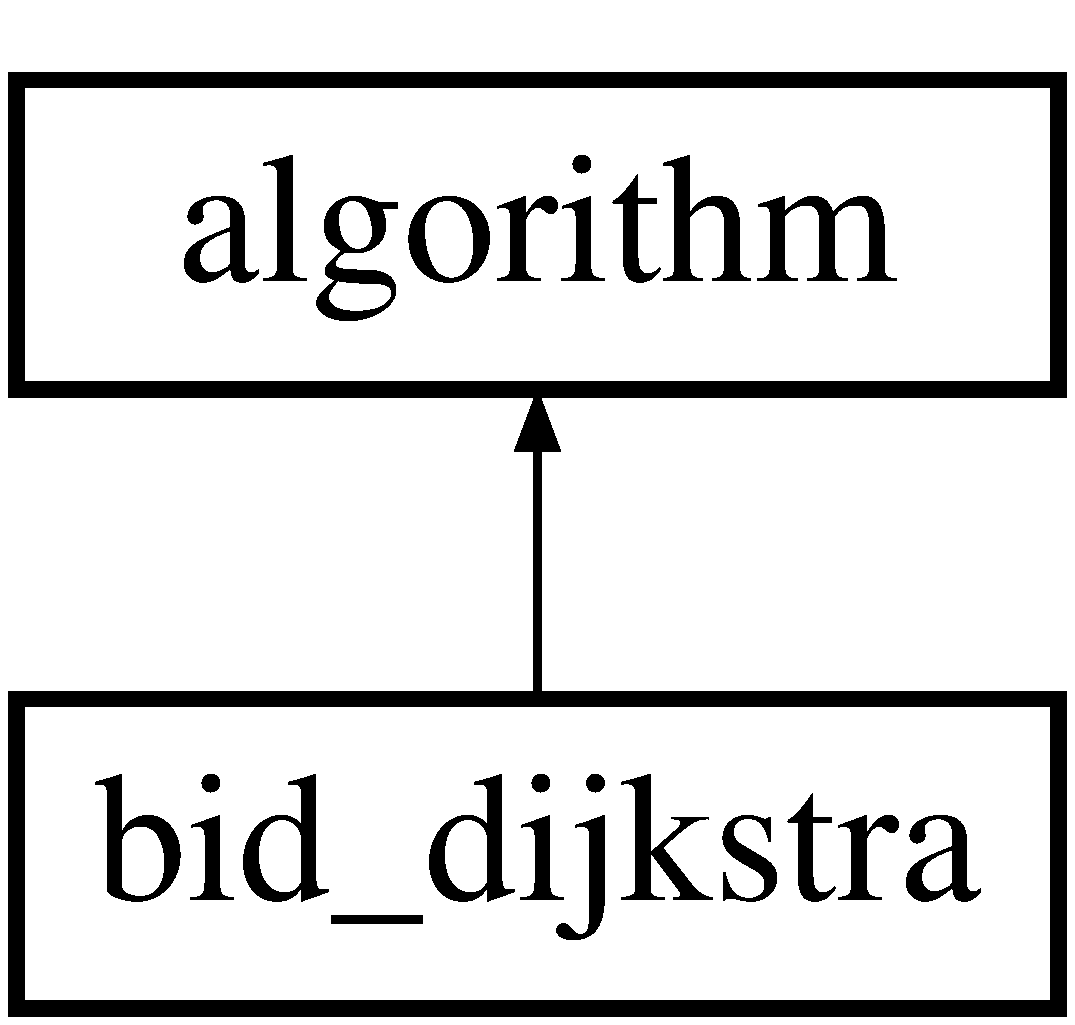
\includegraphics[height=2.000000cm]{classbid__dijkstra}
\end{center}
\end{figure}
\subsection*{Public Types}
\begin{DoxyCompactItemize}
\item 
\mbox{\Hypertarget{classbid__dijkstra_a8b7dcccc9fab2ec5edc8da01029c09d5}\label{classbid__dijkstra_a8b7dcccc9fab2ec5edc8da01029c09d5}} 
enum {\bfseries node\+\_\+color} \{ {\bfseries white}, 
{\bfseries grey}, 
{\bfseries black}
 \}
\item 
\mbox{\Hypertarget{classbid__dijkstra_ada2e642d9f0582d30fe1dd51c4aa1899}\label{classbid__dijkstra_ada2e642d9f0582d30fe1dd51c4aa1899}} 
typedef list$<$ \mbox{\hyperlink{classnode}{node}} $>$\+::const\+\_\+iterator \mbox{\hyperlink{classbid__dijkstra_ada2e642d9f0582d30fe1dd51c4aa1899}{shortest\+\_\+path\+\_\+node\+\_\+iterator}}
\begin{DoxyCompactList}\small\item\em Iterator type for traversing nodes on one shortest path. \end{DoxyCompactList}\item 
\mbox{\Hypertarget{classbid__dijkstra_a703d0faf9568bc25a9305faa61412fe1}\label{classbid__dijkstra_a703d0faf9568bc25a9305faa61412fe1}} 
typedef list$<$ \mbox{\hyperlink{classedge}{edge}} $>$\+::const\+\_\+iterator \mbox{\hyperlink{classbid__dijkstra_a703d0faf9568bc25a9305faa61412fe1}{shortest\+\_\+path\+\_\+edge\+\_\+iterator}}
\begin{DoxyCompactList}\small\item\em Iterator type for traversing edges on one shortest path. \end{DoxyCompactList}\end{DoxyCompactItemize}
\subsection*{Public Member Functions}
\begin{DoxyCompactItemize}
\item 
\mbox{\hyperlink{classbid__dijkstra_a1f9ddd95b88b24f45afe0966c2ae181b}{bid\+\_\+dijkstra}} ()
\begin{DoxyCompactList}\small\item\em Default constructor. \end{DoxyCompactList}\item 
virtual \mbox{\hyperlink{classbid__dijkstra_a3d46b327a3a87ac874e3930227a13757}{$\sim$bid\+\_\+dijkstra}} ()
\begin{DoxyCompactList}\small\item\em Destructor. \end{DoxyCompactList}\item 
void \mbox{\hyperlink{classbid__dijkstra_a25dfbd432043e2e642e4dc71f4cb3208}{source\+\_\+target}} (const \mbox{\hyperlink{classnode}{node}} \&s, const \mbox{\hyperlink{classnode}{node}} \&t)
\begin{DoxyCompactList}\small\item\em Sets source and target node. \end{DoxyCompactList}\item 
void \mbox{\hyperlink{classbid__dijkstra_a33dd3a1cc5eb156b56a72235c9140e7d}{weights}} (const \mbox{\hyperlink{classedge__map}{edge\+\_\+map}}$<$ double $>$ \&weight)
\begin{DoxyCompactList}\small\item\em Sets weights of the edges. \end{DoxyCompactList}\item 
void \mbox{\hyperlink{classbid__dijkstra_a0032d9b44c8b3f6f5733ff3ef94cf169}{store\+\_\+path}} (bool set)
\begin{DoxyCompactList}\small\item\em Enables or disables the storing of the shortest path. \end{DoxyCompactList}\item 
virtual int \mbox{\hyperlink{classbid__dijkstra_a504aa04d114f27f2f886ee3b025ad95b}{check}} (\mbox{\hyperlink{classgraph}{graph}} \&G)
\begin{DoxyCompactList}\small\item\em Checks whether the preconditions for bidirectional Dijkstra are satisfied. \end{DoxyCompactList}\item 
int \mbox{\hyperlink{classbid__dijkstra_a1d2f36d3977ef90285442a269a03b919}{run}} (\mbox{\hyperlink{classgraph}{graph}} \&G)
\begin{DoxyCompactList}\small\item\em Runs shortest path algorithm on {\ttfamily G}. \end{DoxyCompactList}\item 
\mbox{\hyperlink{classnode}{node}} \mbox{\hyperlink{classbid__dijkstra_ae8f5268e008b003e38f25c83ed3fd138}{source}} () const
\begin{DoxyCompactList}\small\item\em Returns source node. \end{DoxyCompactList}\item 
\mbox{\hyperlink{classnode}{node}} \mbox{\hyperlink{classbid__dijkstra_a5d32d74a93c1be5581f56ba3a2839ff5}{target}} () const
\begin{DoxyCompactList}\small\item\em Returns target node if set, {\ttfamily \mbox{\hyperlink{classnode_ad603259398d5667e3b97a6322a2bcc20}{node\+::node()}}} else. \end{DoxyCompactList}\item 
bool \mbox{\hyperlink{classbid__dijkstra_ad9716d8f542f07e5696aba778417cc12}{store\+\_\+path}} () const
\begin{DoxyCompactList}\small\item\em Returns whether the storing of the shortest path is enabled. \end{DoxyCompactList}\item 
bool \mbox{\hyperlink{classbid__dijkstra_a97f599b54fe9b030d87474898ff4a64c}{reached}} () const
\begin{DoxyCompactList}\small\item\em Returns whether target is reachable from source. \end{DoxyCompactList}\item 
double \mbox{\hyperlink{classbid__dijkstra_a6150beb75d59f16d0332f42d5ff7e3f3}{distance}} () const
\begin{DoxyCompactList}\small\item\em Returns the distance from source node to target node. \end{DoxyCompactList}\item 
\mbox{\hyperlink{classbid__dijkstra_ada2e642d9f0582d30fe1dd51c4aa1899}{shortest\+\_\+path\+\_\+node\+\_\+iterator}} \mbox{\hyperlink{classbid__dijkstra_a03807bf76c9a75f0e17e79d20d73f48d}{shortest\+\_\+path\+\_\+nodes\+\_\+begin}} ()
\begin{DoxyCompactList}\small\item\em Returns an iterator to the beginning (to the source node) of the shortest node path to target node. \end{DoxyCompactList}\item 
\mbox{\hyperlink{classbid__dijkstra_ada2e642d9f0582d30fe1dd51c4aa1899}{shortest\+\_\+path\+\_\+node\+\_\+iterator}} \mbox{\hyperlink{classbid__dijkstra_af06035d39e06a70a1c44f1c60c347c5a}{shortest\+\_\+path\+\_\+nodes\+\_\+end}} ()
\begin{DoxyCompactList}\small\item\em Returns an iterator one after the end (one after target node) of the shortest node path to target node. \end{DoxyCompactList}\item 
\mbox{\hyperlink{classbid__dijkstra_a703d0faf9568bc25a9305faa61412fe1}{shortest\+\_\+path\+\_\+edge\+\_\+iterator}} \mbox{\hyperlink{classbid__dijkstra_a177bf7ffd4bf83ce364076ab5183dc3e}{shortest\+\_\+path\+\_\+edges\+\_\+begin}} ()
\begin{DoxyCompactList}\small\item\em Returns an iterator to the beginning edge of the shortest edge path to target node. \end{DoxyCompactList}\item 
\mbox{\hyperlink{classbid__dijkstra_a703d0faf9568bc25a9305faa61412fe1}{shortest\+\_\+path\+\_\+edge\+\_\+iterator}} \mbox{\hyperlink{classbid__dijkstra_a0c31fda13205cd7905ff2400c60bb5e2}{shortest\+\_\+path\+\_\+edges\+\_\+end}} ()
\begin{DoxyCompactList}\small\item\em Returns an iterator one after the end of a shortest edge path to target node. \end{DoxyCompactList}\item 
virtual void \mbox{\hyperlink{classbid__dijkstra_a6df2769941bc73fc5626b084745a2258}{reset}} ()
\begin{DoxyCompactList}\small\item\em Resets Dijkstra\textquotesingle{}s bidirectional algorithm. \end{DoxyCompactList}\end{DoxyCompactItemize}


\subsection{Detailed Description}
Dijkstra\textquotesingle{}s Algorithm for computing a shortest path from a single source to a single target. 

\begin{DoxyParagraph}{Date}
2019/05/07 15\+:58\+:54 
\end{DoxyParagraph}
\begin{DoxyParagraph}{Revision}
1.\+3 
\end{DoxyParagraph}


This class implements Dijkstra\textquotesingle{}s algorithm in a bidirectional manner for computing a shortest path from a single source to a single target in $\mathcal{O}((|V| + |E|) log |V|)$ worst case.

\begin{DoxySeeAlso}{See also}
\mbox{\hyperlink{classdijkstra}{dijkstra}} 

\mbox{\hyperlink{classbellman__ford}{bellman\+\_\+ford}}
\end{DoxySeeAlso}
\begin{DoxyAuthor}{Author}
Stf Kolev \href{mailto:inkyzfx@gmail.com}{\tt inkyzfx@gmail.\+com} 
\end{DoxyAuthor}


\subsection{Constructor \& Destructor Documentation}
\mbox{\Hypertarget{classbid__dijkstra_a1f9ddd95b88b24f45afe0966c2ae181b}\label{classbid__dijkstra_a1f9ddd95b88b24f45afe0966c2ae181b}} 
\index{bid\+\_\+dijkstra@{bid\+\_\+dijkstra}!bid\+\_\+dijkstra@{bid\+\_\+dijkstra}}
\index{bid\+\_\+dijkstra@{bid\+\_\+dijkstra}!bid\+\_\+dijkstra@{bid\+\_\+dijkstra}}
\subsubsection{\texorpdfstring{bid\+\_\+dijkstra()}{bid\_dijkstra()}}
{\footnotesize\ttfamily bid\+\_\+dijkstra\+::bid\+\_\+dijkstra (\begin{DoxyParamCaption}{ }\end{DoxyParamCaption})}



Default constructor. 

Enables only the calculation of shortest paths.

\begin{DoxySeeAlso}{See also}
\mbox{\hyperlink{classalgorithm_ab79e1ddec2f2afdf4b36b10724db8b15}{algorithm\+::algorithm}} 
\end{DoxySeeAlso}
\mbox{\Hypertarget{classbid__dijkstra_a3d46b327a3a87ac874e3930227a13757}\label{classbid__dijkstra_a3d46b327a3a87ac874e3930227a13757}} 
\index{bid\+\_\+dijkstra@{bid\+\_\+dijkstra}!````~bid\+\_\+dijkstra@{$\sim$bid\+\_\+dijkstra}}
\index{````~bid\+\_\+dijkstra@{$\sim$bid\+\_\+dijkstra}!bid\+\_\+dijkstra@{bid\+\_\+dijkstra}}
\subsubsection{\texorpdfstring{$\sim$bid\+\_\+dijkstra()}{~bid\_dijkstra()}}
{\footnotesize\ttfamily bid\+\_\+dijkstra\+::$\sim$bid\+\_\+dijkstra (\begin{DoxyParamCaption}{ }\end{DoxyParamCaption})\hspace{0.3cm}{\ttfamily [virtual]}}



Destructor. 

\begin{DoxySeeAlso}{See also}
\mbox{\hyperlink{classalgorithm_adca9b1e7fa3afd914519a9dbb44e9fd5}{algorithm\+::$\sim$algorithm}} 
\end{DoxySeeAlso}


\subsection{Member Function Documentation}
\mbox{\Hypertarget{classbid__dijkstra_a504aa04d114f27f2f886ee3b025ad95b}\label{classbid__dijkstra_a504aa04d114f27f2f886ee3b025ad95b}} 
\index{bid\+\_\+dijkstra@{bid\+\_\+dijkstra}!check@{check}}
\index{check@{check}!bid\+\_\+dijkstra@{bid\+\_\+dijkstra}}
\subsubsection{\texorpdfstring{check()}{check()}}
{\footnotesize\ttfamily int bid\+\_\+dijkstra\+::check (\begin{DoxyParamCaption}\item[{\mbox{\hyperlink{classgraph}{graph}} \&}]{G }\end{DoxyParamCaption})\hspace{0.3cm}{\ttfamily [virtual]}}



Checks whether the preconditions for bidirectional Dijkstra are satisfied. 

The Precondition are that the weights of the edges have been set and that the graph has at least one node. Additionally all edge weights must be $\ge 0$ and and source and target nodes must be found in {\ttfamily G}.


\begin{DoxyParams}{Parameters}
{\em G} & graph\\
\hline
\end{DoxyParams}

\begin{DoxyRetVals}{Return values}
{\em \mbox{\hyperlink{classalgorithm_af1a0078e153aa99c24f9bdf0d97f6710aae4c1cd7fe8d8cf4b143241a6e7c31cf}{algorithm\+::\+K\+G\+L\+\_\+\+OK}}} & if algorithm can be applied \\
\hline
{\em \mbox{\hyperlink{classalgorithm_af1a0078e153aa99c24f9bdf0d97f6710ae67bf27b2ef31f73e545a7f9f4a69556}{algorithm\+::\+K\+G\+L\+\_\+\+E\+R\+R\+OR}}} & otherwise\\
\hline
\end{DoxyRetVals}
\begin{DoxySeeAlso}{See also}
\mbox{\hyperlink{classdijkstra_a9689f2628f76ddb3747ea18c91bd7041}{dijkstra\+::source}} 

dijkstra\+::weigths 

\mbox{\hyperlink{classalgorithm_a76361fb03ad1cf643affc51821e43bed}{algorithm\+::check}} 
\end{DoxySeeAlso}


Implements \mbox{\hyperlink{classalgorithm_a76361fb03ad1cf643affc51821e43bed}{algorithm}}.

\mbox{\Hypertarget{classbid__dijkstra_a6150beb75d59f16d0332f42d5ff7e3f3}\label{classbid__dijkstra_a6150beb75d59f16d0332f42d5ff7e3f3}} 
\index{bid\+\_\+dijkstra@{bid\+\_\+dijkstra}!distance@{distance}}
\index{distance@{distance}!bid\+\_\+dijkstra@{bid\+\_\+dijkstra}}
\subsubsection{\texorpdfstring{distance()}{distance()}}
{\footnotesize\ttfamily double bid\+\_\+dijkstra\+::distance (\begin{DoxyParamCaption}{ }\end{DoxyParamCaption}) const}



Returns the distance from source node to target node. 

\begin{DoxyReturn}{Returns}
distance if target is \mbox{\hyperlink{classbid__dijkstra_a97f599b54fe9b030d87474898ff4a64c}{bid\+\_\+dijkstra\+::reached}}, {\ttfamily -\/1.\+0} else 
\end{DoxyReturn}
\mbox{\Hypertarget{classbid__dijkstra_a97f599b54fe9b030d87474898ff4a64c}\label{classbid__dijkstra_a97f599b54fe9b030d87474898ff4a64c}} 
\index{bid\+\_\+dijkstra@{bid\+\_\+dijkstra}!reached@{reached}}
\index{reached@{reached}!bid\+\_\+dijkstra@{bid\+\_\+dijkstra}}
\subsubsection{\texorpdfstring{reached()}{reached()}}
{\footnotesize\ttfamily bool bid\+\_\+dijkstra\+::reached (\begin{DoxyParamCaption}{ }\end{DoxyParamCaption}) const}



Returns whether target is reachable from source. 

\begin{DoxyReturn}{Returns}
{\ttfamily true} iff target was reached from source 
\end{DoxyReturn}
\mbox{\Hypertarget{classbid__dijkstra_a6df2769941bc73fc5626b084745a2258}\label{classbid__dijkstra_a6df2769941bc73fc5626b084745a2258}} 
\index{bid\+\_\+dijkstra@{bid\+\_\+dijkstra}!reset@{reset}}
\index{reset@{reset}!bid\+\_\+dijkstra@{bid\+\_\+dijkstra}}
\subsubsection{\texorpdfstring{reset()}{reset()}}
{\footnotesize\ttfamily void bid\+\_\+dijkstra\+::reset (\begin{DoxyParamCaption}{ }\end{DoxyParamCaption})\hspace{0.3cm}{\ttfamily [virtual]}}



Resets Dijkstra\textquotesingle{}s bidirectional algorithm. 

It prepares the algorithm to be applied again, possibly to another graph.

\begin{DoxyNote}{Note}
The weights are not reset. You can apply this algorithms
\end{DoxyNote}
\begin{DoxySeeAlso}{See also}
\mbox{\hyperlink{classalgorithm_a21aba63d066ae7897de6ca7d8425c408}{algorithm\+::reset}} 
\end{DoxySeeAlso}


Implements \mbox{\hyperlink{classalgorithm_a21aba63d066ae7897de6ca7d8425c408}{algorithm}}.

\mbox{\Hypertarget{classbid__dijkstra_a1d2f36d3977ef90285442a269a03b919}\label{classbid__dijkstra_a1d2f36d3977ef90285442a269a03b919}} 
\index{bid\+\_\+dijkstra@{bid\+\_\+dijkstra}!run@{run}}
\index{run@{run}!bid\+\_\+dijkstra@{bid\+\_\+dijkstra}}
\subsubsection{\texorpdfstring{run()}{run()}}
{\footnotesize\ttfamily int bid\+\_\+dijkstra\+::run (\begin{DoxyParamCaption}\item[{\mbox{\hyperlink{classgraph}{graph}} \&}]{G }\end{DoxyParamCaption})\hspace{0.3cm}{\ttfamily [virtual]}}



Runs shortest path algorithm on {\ttfamily G}. 

This should return always \mbox{\hyperlink{classalgorithm_af1a0078e153aa99c24f9bdf0d97f6710aae4c1cd7fe8d8cf4b143241a6e7c31cf}{algorithm\+::\+K\+G\+L\+\_\+\+OK}}. The return value only tracks errors that might occur. Afterwards the result of the test can be accessed via access methods.


\begin{DoxyParams}{Parameters}
{\em G} & graph\\
\hline
\end{DoxyParams}

\begin{DoxyRetVals}{Return values}
{\em \mbox{\hyperlink{classalgorithm_af1a0078e153aa99c24f9bdf0d97f6710aae4c1cd7fe8d8cf4b143241a6e7c31cf}{algorithm\+::\+K\+G\+L\+\_\+\+OK}}} & on success \\
\hline
{\em \mbox{\hyperlink{classalgorithm_af1a0078e153aa99c24f9bdf0d97f6710ae67bf27b2ef31f73e545a7f9f4a69556}{algorithm\+::\+K\+G\+L\+\_\+\+E\+R\+R\+OR}}} & otherwise\\
\hline
\end{DoxyRetVals}
\begin{DoxySeeAlso}{See also}
\mbox{\hyperlink{classalgorithm_a734b189509a8d6b56b65f8ff772d43ca}{algorithm\+::run}} 
\end{DoxySeeAlso}


Implements \mbox{\hyperlink{classalgorithm_a734b189509a8d6b56b65f8ff772d43ca}{algorithm}}.

\mbox{\Hypertarget{classbid__dijkstra_a177bf7ffd4bf83ce364076ab5183dc3e}\label{classbid__dijkstra_a177bf7ffd4bf83ce364076ab5183dc3e}} 
\index{bid\+\_\+dijkstra@{bid\+\_\+dijkstra}!shortest\+\_\+path\+\_\+edges\+\_\+begin@{shortest\+\_\+path\+\_\+edges\+\_\+begin}}
\index{shortest\+\_\+path\+\_\+edges\+\_\+begin@{shortest\+\_\+path\+\_\+edges\+\_\+begin}!bid\+\_\+dijkstra@{bid\+\_\+dijkstra}}
\subsubsection{\texorpdfstring{shortest\+\_\+path\+\_\+edges\+\_\+begin()}{shortest\_path\_edges\_begin()}}
{\footnotesize\ttfamily \mbox{\hyperlink{classbid__dijkstra_a703d0faf9568bc25a9305faa61412fe1}{bid\+\_\+dijkstra\+::shortest\+\_\+path\+\_\+edge\+\_\+iterator}} bid\+\_\+dijkstra\+::shortest\+\_\+path\+\_\+edges\+\_\+begin (\begin{DoxyParamCaption}{ }\end{DoxyParamCaption})}



Returns an iterator to the beginning edge of the shortest edge path to target node. 

\begin{DoxySeeAlso}{See also}
\mbox{\hyperlink{classbid__dijkstra_a0032d9b44c8b3f6f5733ff3ef94cf169}{bid\+\_\+dijkstra\+::store\+\_\+path}}
\end{DoxySeeAlso}
\begin{DoxyReturn}{Returns}
beginning edge iterator of the shortest path
\end{DoxyReturn}
\begin{DoxyNote}{Note}
The method requires that path calculation option was enabled during last run. 
\end{DoxyNote}
\mbox{\Hypertarget{classbid__dijkstra_a0c31fda13205cd7905ff2400c60bb5e2}\label{classbid__dijkstra_a0c31fda13205cd7905ff2400c60bb5e2}} 
\index{bid\+\_\+dijkstra@{bid\+\_\+dijkstra}!shortest\+\_\+path\+\_\+edges\+\_\+end@{shortest\+\_\+path\+\_\+edges\+\_\+end}}
\index{shortest\+\_\+path\+\_\+edges\+\_\+end@{shortest\+\_\+path\+\_\+edges\+\_\+end}!bid\+\_\+dijkstra@{bid\+\_\+dijkstra}}
\subsubsection{\texorpdfstring{shortest\+\_\+path\+\_\+edges\+\_\+end()}{shortest\_path\_edges\_end()}}
{\footnotesize\ttfamily \mbox{\hyperlink{classbid__dijkstra_a703d0faf9568bc25a9305faa61412fe1}{bid\+\_\+dijkstra\+::shortest\+\_\+path\+\_\+edge\+\_\+iterator}} bid\+\_\+dijkstra\+::shortest\+\_\+path\+\_\+edges\+\_\+end (\begin{DoxyParamCaption}{ }\end{DoxyParamCaption})}



Returns an iterator one after the end of a shortest edge path to target node. 

\begin{DoxySeeAlso}{See also}
\mbox{\hyperlink{classbid__dijkstra_a0032d9b44c8b3f6f5733ff3ef94cf169}{bid\+\_\+dijkstra\+::store\+\_\+path}}
\end{DoxySeeAlso}
\begin{DoxyReturn}{Returns}
shortest path end edge iterator
\end{DoxyReturn}
\begin{DoxyNote}{Note}
The method requires that predecessor calculation option was enabled during last run. 
\end{DoxyNote}
\mbox{\Hypertarget{classbid__dijkstra_a03807bf76c9a75f0e17e79d20d73f48d}\label{classbid__dijkstra_a03807bf76c9a75f0e17e79d20d73f48d}} 
\index{bid\+\_\+dijkstra@{bid\+\_\+dijkstra}!shortest\+\_\+path\+\_\+nodes\+\_\+begin@{shortest\+\_\+path\+\_\+nodes\+\_\+begin}}
\index{shortest\+\_\+path\+\_\+nodes\+\_\+begin@{shortest\+\_\+path\+\_\+nodes\+\_\+begin}!bid\+\_\+dijkstra@{bid\+\_\+dijkstra}}
\subsubsection{\texorpdfstring{shortest\+\_\+path\+\_\+nodes\+\_\+begin()}{shortest\_path\_nodes\_begin()}}
{\footnotesize\ttfamily \mbox{\hyperlink{classbid__dijkstra_ada2e642d9f0582d30fe1dd51c4aa1899}{bid\+\_\+dijkstra\+::shortest\+\_\+path\+\_\+node\+\_\+iterator}} bid\+\_\+dijkstra\+::shortest\+\_\+path\+\_\+nodes\+\_\+begin (\begin{DoxyParamCaption}{ }\end{DoxyParamCaption})}



Returns an iterator to the beginning (to the source node) of the shortest node path to target node. 

\begin{DoxyReturn}{Returns}
beginning node iterator of the shortest path
\end{DoxyReturn}
\begin{DoxySeeAlso}{See also}
\mbox{\hyperlink{classbid__dijkstra_a0032d9b44c8b3f6f5733ff3ef94cf169}{bid\+\_\+dijkstra\+::store\+\_\+path}}
\end{DoxySeeAlso}
\begin{DoxyNote}{Note}
The method requires that path calculation option was enabled during last run. 
\end{DoxyNote}
\mbox{\Hypertarget{classbid__dijkstra_af06035d39e06a70a1c44f1c60c347c5a}\label{classbid__dijkstra_af06035d39e06a70a1c44f1c60c347c5a}} 
\index{bid\+\_\+dijkstra@{bid\+\_\+dijkstra}!shortest\+\_\+path\+\_\+nodes\+\_\+end@{shortest\+\_\+path\+\_\+nodes\+\_\+end}}
\index{shortest\+\_\+path\+\_\+nodes\+\_\+end@{shortest\+\_\+path\+\_\+nodes\+\_\+end}!bid\+\_\+dijkstra@{bid\+\_\+dijkstra}}
\subsubsection{\texorpdfstring{shortest\+\_\+path\+\_\+nodes\+\_\+end()}{shortest\_path\_nodes\_end()}}
{\footnotesize\ttfamily \mbox{\hyperlink{classbid__dijkstra_ada2e642d9f0582d30fe1dd51c4aa1899}{bid\+\_\+dijkstra\+::shortest\+\_\+path\+\_\+node\+\_\+iterator}} bid\+\_\+dijkstra\+::shortest\+\_\+path\+\_\+nodes\+\_\+end (\begin{DoxyParamCaption}{ }\end{DoxyParamCaption})}



Returns an iterator one after the end (one after target node) of the shortest node path to target node. 

\begin{DoxyReturn}{Returns}
shortest path end node iterator
\end{DoxyReturn}
\begin{DoxySeeAlso}{See also}
\mbox{\hyperlink{classbid__dijkstra_a0032d9b44c8b3f6f5733ff3ef94cf169}{bid\+\_\+dijkstra\+::store\+\_\+path}}
\end{DoxySeeAlso}
\begin{DoxyNote}{Note}
The method requires that path calculation option was enabled during last run. 
\end{DoxyNote}
\mbox{\Hypertarget{classbid__dijkstra_ae8f5268e008b003e38f25c83ed3fd138}\label{classbid__dijkstra_ae8f5268e008b003e38f25c83ed3fd138}} 
\index{bid\+\_\+dijkstra@{bid\+\_\+dijkstra}!source@{source}}
\index{source@{source}!bid\+\_\+dijkstra@{bid\+\_\+dijkstra}}
\subsubsection{\texorpdfstring{source()}{source()}}
{\footnotesize\ttfamily \mbox{\hyperlink{classnode}{node}} bid\+\_\+dijkstra\+::source (\begin{DoxyParamCaption}{ }\end{DoxyParamCaption}) const}



Returns source node. 

\begin{DoxyReturn}{Returns}
source node 
\end{DoxyReturn}
\mbox{\Hypertarget{classbid__dijkstra_a25dfbd432043e2e642e4dc71f4cb3208}\label{classbid__dijkstra_a25dfbd432043e2e642e4dc71f4cb3208}} 
\index{bid\+\_\+dijkstra@{bid\+\_\+dijkstra}!source\+\_\+target@{source\+\_\+target}}
\index{source\+\_\+target@{source\+\_\+target}!bid\+\_\+dijkstra@{bid\+\_\+dijkstra}}
\subsubsection{\texorpdfstring{source\+\_\+target()}{source\_target()}}
{\footnotesize\ttfamily void bid\+\_\+dijkstra\+::source\+\_\+target (\begin{DoxyParamCaption}\item[{const \mbox{\hyperlink{classnode}{node}} \&}]{s,  }\item[{const \mbox{\hyperlink{classnode}{node}} \&}]{t }\end{DoxyParamCaption})}



Sets source and target node. 

Must be executed every time before check and run of this algorithm.


\begin{DoxyParams}{Parameters}
{\em s} & source node \\
\hline
{\em t} & target node \\
\hline
\end{DoxyParams}
\mbox{\Hypertarget{classbid__dijkstra_a0032d9b44c8b3f6f5733ff3ef94cf169}\label{classbid__dijkstra_a0032d9b44c8b3f6f5733ff3ef94cf169}} 
\index{bid\+\_\+dijkstra@{bid\+\_\+dijkstra}!store\+\_\+path@{store\+\_\+path}}
\index{store\+\_\+path@{store\+\_\+path}!bid\+\_\+dijkstra@{bid\+\_\+dijkstra}}
\subsubsection{\texorpdfstring{store\+\_\+path()}{store\_path()}\hspace{0.1cm}{\footnotesize\ttfamily [1/2]}}
{\footnotesize\ttfamily void bid\+\_\+dijkstra\+::store\+\_\+path (\begin{DoxyParamCaption}\item[{bool}]{set }\end{DoxyParamCaption})}



Enables or disables the storing of the shortest path. 

If enabled for every node and edge on the shortest path from source to target will be stored.


\begin{DoxyParams}{Parameters}
{\em set} & true if path should be stored\\
\hline
\end{DoxyParams}
\begin{DoxySeeAlso}{See also}
\mbox{\hyperlink{classdijkstra_a99c17ee7c2b55574ea8c2952fac09faf}{dijkstra\+::predecessor\+\_\+node}} 

\mbox{\hyperlink{classdijkstra_aa3ef1a7d7dfc33e4a39aff309f873929}{dijkstra\+::predecessor\+\_\+edge}} 
\end{DoxySeeAlso}
\mbox{\Hypertarget{classbid__dijkstra_ad9716d8f542f07e5696aba778417cc12}\label{classbid__dijkstra_ad9716d8f542f07e5696aba778417cc12}} 
\index{bid\+\_\+dijkstra@{bid\+\_\+dijkstra}!store\+\_\+path@{store\+\_\+path}}
\index{store\+\_\+path@{store\+\_\+path}!bid\+\_\+dijkstra@{bid\+\_\+dijkstra}}
\subsubsection{\texorpdfstring{store\+\_\+path()}{store\_path()}\hspace{0.1cm}{\footnotesize\ttfamily [2/2]}}
{\footnotesize\ttfamily bool bid\+\_\+dijkstra\+::store\+\_\+path (\begin{DoxyParamCaption}{ }\end{DoxyParamCaption}) const}



Returns whether the storing of the shortest path is enabled. 

\begin{DoxyReturn}{Returns}
{\ttfamily true} iff the storing of path is enabled.
\end{DoxyReturn}
\begin{DoxySeeAlso}{See also}
dijkstra\+::predecessor 
\end{DoxySeeAlso}
\mbox{\Hypertarget{classbid__dijkstra_a5d32d74a93c1be5581f56ba3a2839ff5}\label{classbid__dijkstra_a5d32d74a93c1be5581f56ba3a2839ff5}} 
\index{bid\+\_\+dijkstra@{bid\+\_\+dijkstra}!target@{target}}
\index{target@{target}!bid\+\_\+dijkstra@{bid\+\_\+dijkstra}}
\subsubsection{\texorpdfstring{target()}{target()}}
{\footnotesize\ttfamily \mbox{\hyperlink{classnode}{node}} bid\+\_\+dijkstra\+::target (\begin{DoxyParamCaption}{ }\end{DoxyParamCaption}) const}



Returns target node if set, {\ttfamily \mbox{\hyperlink{classnode_ad603259398d5667e3b97a6322a2bcc20}{node\+::node()}}} else. 

\begin{DoxyReturn}{Returns}
target node 
\end{DoxyReturn}
\mbox{\Hypertarget{classbid__dijkstra_a33dd3a1cc5eb156b56a72235c9140e7d}\label{classbid__dijkstra_a33dd3a1cc5eb156b56a72235c9140e7d}} 
\index{bid\+\_\+dijkstra@{bid\+\_\+dijkstra}!weights@{weights}}
\index{weights@{weights}!bid\+\_\+dijkstra@{bid\+\_\+dijkstra}}
\subsubsection{\texorpdfstring{weights()}{weights()}}
{\footnotesize\ttfamily void bid\+\_\+dijkstra\+::weights (\begin{DoxyParamCaption}\item[{const \mbox{\hyperlink{classedge__map}{edge\+\_\+map}}$<$ double $>$ \&}]{weight }\end{DoxyParamCaption})}



Sets weights of the edges. 

This method {\bfseries must} be called before check and run.


\begin{DoxyParams}{Parameters}
{\em weight} & weights of the edges \\
\hline
\end{DoxyParams}


The documentation for this class was generated from the following files\+:\begin{DoxyCompactItemize}
\item 
include/\+K\+G\+L/bid\+\_\+dijkstra.\+h\item 
src/bid\+\_\+dijkstra.\+cpp\end{DoxyCompactItemize}

\hypertarget{classbin__heap}{}\section{bin\+\_\+heap$<$ T, Pred $>$ Class Template Reference}
\label{classbin__heap}\index{bin\+\_\+heap$<$ T, Pred $>$@{bin\+\_\+heap$<$ T, Pred $>$}}


Binary heap.  




{\ttfamily \#include $<$bin\+\_\+heap.\+h$>$}

\subsection*{Public Member Functions}
\begin{DoxyCompactItemize}
\item 
\mbox{\hyperlink{classbin__heap_a9de42b60fac4b0d38aa738522eb7c4cd}{bin\+\_\+heap}} (const Pred \&prd)
\begin{DoxyCompactList}\small\item\em Creates empty binary heap. \end{DoxyCompactList}\item 
\mbox{\hyperlink{classbin__heap_ab911dd559d9d9fd665b9fdf2d8202bb8}{bin\+\_\+heap}} (const Pred \&prd, const int est\+\_\+size)
\begin{DoxyCompactList}\small\item\em Creates empty binary heap. \end{DoxyCompactList}\item 
\mbox{\hyperlink{classbin__heap_a19bd4241e097852ffda83b72557ffbdc}{bin\+\_\+heap}} (const \mbox{\hyperlink{classbin__heap}{bin\+\_\+heap}}$<$ T, Pred $>$ \&bh)
\begin{DoxyCompactList}\small\item\em Copy constructor. \end{DoxyCompactList}\item 
\mbox{\hyperlink{classbin__heap}{bin\+\_\+heap}}$<$ T, Pred $>$ \& \mbox{\hyperlink{classbin__heap_ad31b6806316a272686015fcbf5f633cd}{operator=}} (const \mbox{\hyperlink{classbin__heap}{bin\+\_\+heap}}$<$ T, Pred $>$ \&bh)
\begin{DoxyCompactList}\small\item\em Assigns {\ttfamily bh} to this binary heap. \end{DoxyCompactList}\item 
\mbox{\Hypertarget{classbin__heap_a5283db56783a84ee28dea9d393acf905}\label{classbin__heap_a5283db56783a84ee28dea9d393acf905}} 
\mbox{\hyperlink{classbin__heap_a5283db56783a84ee28dea9d393acf905}{$\sim$bin\+\_\+heap}} ()
\begin{DoxyCompactList}\small\item\em Destructor. \end{DoxyCompactList}\item 
void \mbox{\hyperlink{classbin__heap_a6d658d61533e66cf83dce2f8e35bed17}{push}} (const T \&ins)
\begin{DoxyCompactList}\small\item\em Inserts {\ttfamily ins} in heap. \end{DoxyCompactList}\item 
\mbox{\Hypertarget{classbin__heap_ab463bc655b2f46cd5ff021cab28b1210}\label{classbin__heap_ab463bc655b2f46cd5ff021cab28b1210}} 
void \mbox{\hyperlink{classbin__heap_ab463bc655b2f46cd5ff021cab28b1210}{pop}} ()
\begin{DoxyCompactList}\small\item\em Removes the element on top of the heap. \end{DoxyCompactList}\item 
const T \& \mbox{\hyperlink{classbin__heap_acd711ddeafe82630f153906da7e8fa1c}{top}} () const
\begin{DoxyCompactList}\small\item\em Returns a reference to the element at the top of the heap. \end{DoxyCompactList}\item 
void \mbox{\hyperlink{classbin__heap_ab1353fe40c5cfc1205314a4db6334f1b}{change\+Key}} (const T \&cha)
\begin{DoxyCompactList}\small\item\em Reconstructs heap condition after changing key value of {\ttfamily cha} externally. \end{DoxyCompactList}\item 
bool \mbox{\hyperlink{classbin__heap_a2bbb9cf5cc5cda265c8603c561b796a5}{is\+\_\+empty}} () const
\begin{DoxyCompactList}\small\item\em Checks if heap is empty. \end{DoxyCompactList}\item 
\mbox{\Hypertarget{classbin__heap_abf7a6189fcb48e435fc156f764e38f1d}\label{classbin__heap_abf7a6189fcb48e435fc156f764e38f1d}} 
void {\bfseries clear} ()
\end{DoxyCompactItemize}


\subsection{Detailed Description}
\subsubsection*{template$<$class T, class Pred$>$\newline
class bin\+\_\+heap$<$ T, Pred $>$}

Binary heap. 

\begin{DoxyAuthor}{Author}
Stf Kolev \href{mailto:inkyzfx@gmail.com}{\tt inkyzfx@gmail.\+com} 
\end{DoxyAuthor}


\subsection{Constructor \& Destructor Documentation}
\mbox{\Hypertarget{classbin__heap_a9de42b60fac4b0d38aa738522eb7c4cd}\label{classbin__heap_a9de42b60fac4b0d38aa738522eb7c4cd}} 
\index{bin\+\_\+heap@{bin\+\_\+heap}!bin\+\_\+heap@{bin\+\_\+heap}}
\index{bin\+\_\+heap@{bin\+\_\+heap}!bin\+\_\+heap@{bin\+\_\+heap}}
\subsubsection{\texorpdfstring{bin\+\_\+heap()}{bin\_heap()}\hspace{0.1cm}{\footnotesize\ttfamily [1/3]}}
{\footnotesize\ttfamily template$<$class T , class Pred $>$ \\
\mbox{\hyperlink{classbin__heap}{bin\+\_\+heap}}$<$ T, Pred $>$\+::\mbox{\hyperlink{classbin__heap}{bin\+\_\+heap}} (\begin{DoxyParamCaption}\item[{const Pred \&}]{prd }\end{DoxyParamCaption})}



Creates empty binary heap. 


\begin{DoxyParams}{Parameters}
{\em prd} & binary predicate to compare two {\ttfamily T}s \\
\hline
\end{DoxyParams}
\mbox{\Hypertarget{classbin__heap_ab911dd559d9d9fd665b9fdf2d8202bb8}\label{classbin__heap_ab911dd559d9d9fd665b9fdf2d8202bb8}} 
\index{bin\+\_\+heap@{bin\+\_\+heap}!bin\+\_\+heap@{bin\+\_\+heap}}
\index{bin\+\_\+heap@{bin\+\_\+heap}!bin\+\_\+heap@{bin\+\_\+heap}}
\subsubsection{\texorpdfstring{bin\+\_\+heap()}{bin\_heap()}\hspace{0.1cm}{\footnotesize\ttfamily [2/3]}}
{\footnotesize\ttfamily template$<$class T , class Pred $>$ \\
\mbox{\hyperlink{classbin__heap}{bin\+\_\+heap}}$<$ T, Pred $>$\+::\mbox{\hyperlink{classbin__heap}{bin\+\_\+heap}} (\begin{DoxyParamCaption}\item[{const Pred \&}]{prd,  }\item[{const int}]{est\+\_\+size }\end{DoxyParamCaption})}



Creates empty binary heap. 


\begin{DoxyParams}{Parameters}
{\em prd} & binary predicate to compare two {\ttfamily Ts} \\
\hline
{\em est\+\_\+size} & estimated maximal size of heap \\
\hline
\end{DoxyParams}
\mbox{\Hypertarget{classbin__heap_a19bd4241e097852ffda83b72557ffbdc}\label{classbin__heap_a19bd4241e097852ffda83b72557ffbdc}} 
\index{bin\+\_\+heap@{bin\+\_\+heap}!bin\+\_\+heap@{bin\+\_\+heap}}
\index{bin\+\_\+heap@{bin\+\_\+heap}!bin\+\_\+heap@{bin\+\_\+heap}}
\subsubsection{\texorpdfstring{bin\+\_\+heap()}{bin\_heap()}\hspace{0.1cm}{\footnotesize\ttfamily [3/3]}}
{\footnotesize\ttfamily template$<$class T , class Pred $>$ \\
\mbox{\hyperlink{classbin__heap}{bin\+\_\+heap}}$<$ T, Pred $>$\+::\mbox{\hyperlink{classbin__heap}{bin\+\_\+heap}} (\begin{DoxyParamCaption}\item[{const \mbox{\hyperlink{classbin__heap}{bin\+\_\+heap}}$<$ T, Pred $>$ \&}]{bh }\end{DoxyParamCaption})}



Copy constructor. 


\begin{DoxyParams}{Parameters}
{\em bh} & binary heap to copy \\
\hline
\end{DoxyParams}


\subsection{Member Function Documentation}
\mbox{\Hypertarget{classbin__heap_ab1353fe40c5cfc1205314a4db6334f1b}\label{classbin__heap_ab1353fe40c5cfc1205314a4db6334f1b}} 
\index{bin\+\_\+heap@{bin\+\_\+heap}!change\+Key@{change\+Key}}
\index{change\+Key@{change\+Key}!bin\+\_\+heap@{bin\+\_\+heap}}
\subsubsection{\texorpdfstring{change\+Key()}{changeKey()}}
{\footnotesize\ttfamily template$<$class T , class Pred $>$ \\
void \mbox{\hyperlink{classbin__heap}{bin\+\_\+heap}}$<$ T, Pred $>$\+::change\+Key (\begin{DoxyParamCaption}\item[{const T \&}]{cha }\end{DoxyParamCaption})}



Reconstructs heap condition after changing key value of {\ttfamily cha} externally. 


\begin{DoxyParams}{Parameters}
{\em cha} & element with changed key value\\
\hline
\end{DoxyParams}
\begin{DoxyNote}{Note}
{\ttfamily change\+Key} doesn\textquotesingle{}t operate if {\ttfamily cha} is a primitive data structure, because it represents its key value itself, or if one object is stored more than once in the data structure.
\end{DoxyNote}
\begin{DoxySeeAlso}{See also}
\mbox{\hyperlink{classdijkstra}{dijkstra}} 
\end{DoxySeeAlso}
\mbox{\Hypertarget{classbin__heap_a2bbb9cf5cc5cda265c8603c561b796a5}\label{classbin__heap_a2bbb9cf5cc5cda265c8603c561b796a5}} 
\index{bin\+\_\+heap@{bin\+\_\+heap}!is\+\_\+empty@{is\+\_\+empty}}
\index{is\+\_\+empty@{is\+\_\+empty}!bin\+\_\+heap@{bin\+\_\+heap}}
\subsubsection{\texorpdfstring{is\+\_\+empty()}{is\_empty()}}
{\footnotesize\ttfamily template$<$class T , class Pred $>$ \\
bool \mbox{\hyperlink{classbin__heap}{bin\+\_\+heap}}$<$ T, Pred $>$\+::is\+\_\+empty (\begin{DoxyParamCaption}{ }\end{DoxyParamCaption}) const}



Checks if heap is empty. 

\begin{DoxyReturn}{Returns}
{\ttfamily true} iff empty 
\end{DoxyReturn}
\mbox{\Hypertarget{classbin__heap_ad31b6806316a272686015fcbf5f633cd}\label{classbin__heap_ad31b6806316a272686015fcbf5f633cd}} 
\index{bin\+\_\+heap@{bin\+\_\+heap}!operator=@{operator=}}
\index{operator=@{operator=}!bin\+\_\+heap@{bin\+\_\+heap}}
\subsubsection{\texorpdfstring{operator=()}{operator=()}}
{\footnotesize\ttfamily template$<$class T , class Pred $>$ \\
\mbox{\hyperlink{classbin__heap}{bin\+\_\+heap}}$<$ T, Pred $>$ \& \mbox{\hyperlink{classbin__heap}{bin\+\_\+heap}}$<$ T, Pred $>$\+::operator= (\begin{DoxyParamCaption}\item[{const \mbox{\hyperlink{classbin__heap}{bin\+\_\+heap}}$<$ T, Pred $>$ \&}]{bh }\end{DoxyParamCaption})}



Assigns {\ttfamily bh} to this binary heap. 

All elements in this heap will be deleted. The predicate of this heap must be physically the same as the one of {\ttfamily bh}.


\begin{DoxyParams}{Parameters}
{\em bh} & binary heap\\
\hline
\end{DoxyParams}
\begin{DoxyReturn}{Returns}
this heap 
\end{DoxyReturn}
\mbox{\Hypertarget{classbin__heap_a6d658d61533e66cf83dce2f8e35bed17}\label{classbin__heap_a6d658d61533e66cf83dce2f8e35bed17}} 
\index{bin\+\_\+heap@{bin\+\_\+heap}!push@{push}}
\index{push@{push}!bin\+\_\+heap@{bin\+\_\+heap}}
\subsubsection{\texorpdfstring{push()}{push()}}
{\footnotesize\ttfamily template$<$class T , class Pred $>$ \\
void \mbox{\hyperlink{classbin__heap}{bin\+\_\+heap}}$<$ T, Pred $>$\+::push (\begin{DoxyParamCaption}\item[{const T \&}]{ins }\end{DoxyParamCaption})}



Inserts {\ttfamily ins} in heap. 


\begin{DoxyParams}{Parameters}
{\em ins} & data element to be inserted \\
\hline
\end{DoxyParams}
\mbox{\Hypertarget{classbin__heap_acd711ddeafe82630f153906da7e8fa1c}\label{classbin__heap_acd711ddeafe82630f153906da7e8fa1c}} 
\index{bin\+\_\+heap@{bin\+\_\+heap}!top@{top}}
\index{top@{top}!bin\+\_\+heap@{bin\+\_\+heap}}
\subsubsection{\texorpdfstring{top()}{top()}}
{\footnotesize\ttfamily template$<$class T , class Pred $>$ \\
const T \& \mbox{\hyperlink{classbin__heap}{bin\+\_\+heap}}$<$ T, Pred $>$\+::top (\begin{DoxyParamCaption}{ }\end{DoxyParamCaption}) const}



Returns a reference to the element at the top of the heap. 

\begin{DoxyReturn}{Returns}
top element of the heap 
\end{DoxyReturn}


The documentation for this class was generated from the following file\+:\begin{DoxyCompactItemize}
\item 
include/\+K\+G\+L/bin\+\_\+heap.\+h\end{DoxyCompactItemize}

\hypertarget{classcomponents}{}\section{components Class Reference}
\label{classcomponents}\index{components@{components}}


Connected components algorithm.  




{\ttfamily \#include $<$components.\+h$>$}

Inheritance diagram for components\+:\begin{figure}[H]
\begin{center}
\leavevmode
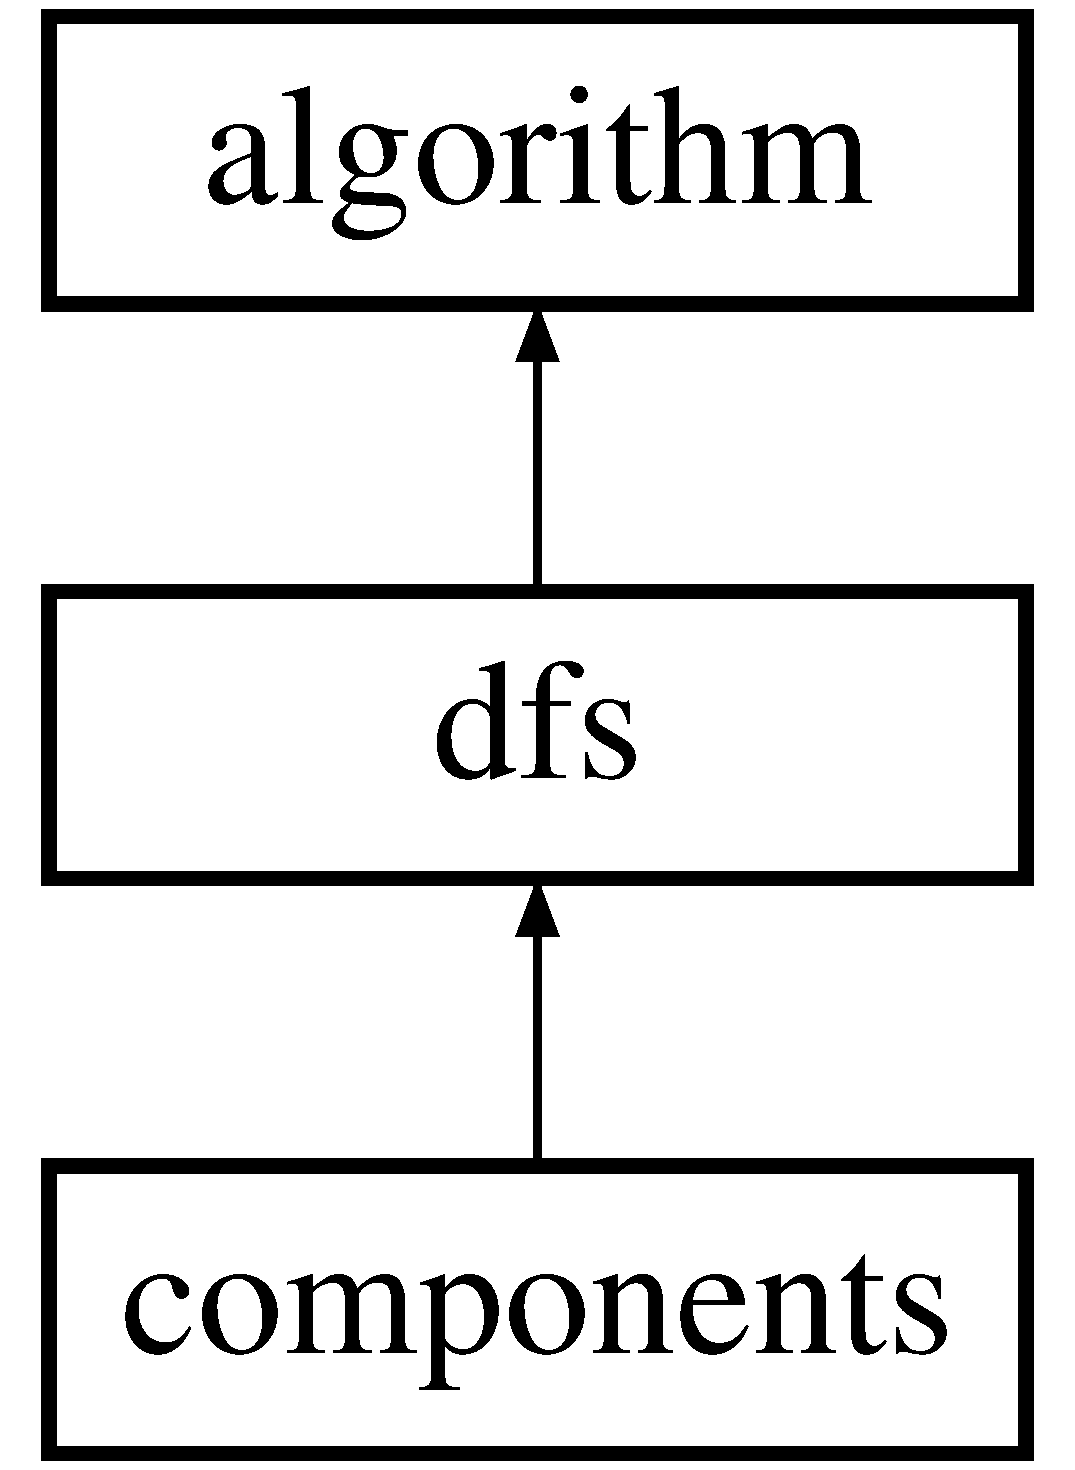
\includegraphics[height=3.000000cm]{classcomponents}
\end{center}
\end{figure}
\subsection*{Public Types}
\begin{DoxyCompactItemize}
\item 
\mbox{\Hypertarget{classcomponents_a5f9e3d26b8f7bc14b8f482754a38cb61}\label{classcomponents_a5f9e3d26b8f7bc14b8f482754a38cb61}} 
typedef list$<$ pair$<$ list$<$ \mbox{\hyperlink{classnode}{node}} $>$, list$<$ \mbox{\hyperlink{classedge}{edge}} $>$ $>$ $>$\+::iterator {\bfseries component\+\_\+iterator}
\end{DoxyCompactItemize}
\subsection*{Public Member Functions}
\begin{DoxyCompactItemize}
\item 
\mbox{\hyperlink{classcomponents_a41b8782301c7985dfa202a04df76712d}{components}} ()
\begin{DoxyCompactList}\small\item\em Creates connected components algorithm object. \end{DoxyCompactList}\item 
virtual \mbox{\hyperlink{classcomponents_aa38e55d08dd484dad3175617264056a5}{$\sim$components}} ()
\begin{DoxyCompactList}\small\item\em Destroys connected components algorithm object. \end{DoxyCompactList}\item 
virtual int \mbox{\hyperlink{classcomponents_aeeda901d02c65d6c31c8b6148540d7c1}{check}} (\mbox{\hyperlink{classgraph}{graph}} \&G)
\begin{DoxyCompactList}\small\item\em Checks whether the connected components algorithm can be applied. \end{DoxyCompactList}\item 
virtual void \mbox{\hyperlink{classcomponents_a07b6bab5962524ae26ccb478b35cd76c}{reset}} ()
\begin{DoxyCompactList}\small\item\em Resets algorithm. \end{DoxyCompactList}\item 
component\+\_\+iterator \mbox{\hyperlink{classcomponents_a8a645639044375cdaefabffda3ae70e0}{components\+\_\+begin}} ()
\begin{DoxyCompactList}\small\item\em Start iteration over all components (if enabled during last call to run). \end{DoxyCompactList}\item 
component\+\_\+iterator \mbox{\hyperlink{classcomponents_a8537c6e4c6a29a4ae05a937b5fda1fb9}{components\+\_\+end}} ()
\begin{DoxyCompactList}\small\item\em End of iteration over all components. \end{DoxyCompactList}\item 
int \mbox{\hyperlink{classcomponents_ad3206d2d050ed7719f7140ea3bee81f8}{number\+\_\+of\+\_\+components}} () const
\begin{DoxyCompactList}\small\item\em Number of components detected during the last run. \end{DoxyCompactList}\item 
virtual void \mbox{\hyperlink{classcomponents_a587a9c44a80deb4260ccd0728bfeab0f}{before\+\_\+recursive\+\_\+call\+\_\+handler}} (\mbox{\hyperlink{classgraph}{graph}} \&, \mbox{\hyperlink{classedge}{edge}} \&, \mbox{\hyperlink{classnode}{node}} \&)
\begin{DoxyCompactList}\small\item\em Handler called when a unused node {\itshape n} connected to the actual node by {\itshape e} is found. \end{DoxyCompactList}\item 
virtual void \mbox{\hyperlink{classcomponents_afcf7a0bee5104bba7986039a9d6bd1ee}{old\+\_\+adj\+\_\+node\+\_\+handler}} (\mbox{\hyperlink{classgraph}{graph}} \&, \mbox{\hyperlink{classedge}{edge}} \&, \mbox{\hyperlink{classnode}{node}} \&)
\begin{DoxyCompactList}\small\item\em Handler called when a already marked node {\itshape n} connected to the actual node by {\itshape e} is found during the search of all adjacent edges of the actual node. \end{DoxyCompactList}\item 
virtual void \mbox{\hyperlink{classcomponents_af53365bd737b34cf63e4a6b10879ffcc}{new\+\_\+start\+\_\+handler}} (\mbox{\hyperlink{classgraph}{graph}} \&, \mbox{\hyperlink{classnode}{node}} \&)
\begin{DoxyCompactList}\small\item\em Called when D\+FS is started with start-\/node {\itshape n}. \end{DoxyCompactList}\end{DoxyCompactItemize}
\subsection*{Protected Attributes}
\begin{DoxyCompactItemize}
\item 
\mbox{\Hypertarget{classcomponents_ad5a54d7313e23f8c6a2c6347e6ee70a0}\label{classcomponents_ad5a54d7313e23f8c6a2c6347e6ee70a0}} 
int {\bfseries num\+\_\+of\+\_\+components}
\item 
\mbox{\Hypertarget{classcomponents_a8ea32e0ef95a2d707b88cfa80209d357}\label{classcomponents_a8ea32e0ef95a2d707b88cfa80209d357}} 
list$<$ pair$<$ list$<$ \mbox{\hyperlink{classnode}{node}} $>$, list$<$ \mbox{\hyperlink{classedge}{edge}} $>$ $>$ $>$ {\bfseries comp}
\item 
\mbox{\Hypertarget{classcomponents_ae88ffb062b1ea4931ecfaa53e871825f}\label{classcomponents_ae88ffb062b1ea4931ecfaa53e871825f}} 
component\+\_\+iterator {\bfseries li}
\end{DoxyCompactItemize}


\subsection{Detailed Description}
Connected components algorithm. 

\subsection{Constructor \& Destructor Documentation}
\mbox{\Hypertarget{classcomponents_a41b8782301c7985dfa202a04df76712d}\label{classcomponents_a41b8782301c7985dfa202a04df76712d}} 
\index{components@{components}!components@{components}}
\index{components@{components}!components@{components}}
\subsubsection{\texorpdfstring{components()}{components()}}
{\footnotesize\ttfamily \+\_\+\+\_\+\+K\+G\+L\+\_\+\+B\+E\+G\+I\+N\+\_\+\+N\+A\+M\+E\+S\+P\+A\+CE components\+::components (\begin{DoxyParamCaption}{ }\end{DoxyParamCaption})}



Creates connected components algorithm object. 

\begin{DoxySeeAlso}{See also}
\mbox{\hyperlink{classdfs_a5232bc41ab202b6278a84bd97c803a0d}{dfs\+::dfs}} 
\end{DoxySeeAlso}
\mbox{\Hypertarget{classcomponents_aa38e55d08dd484dad3175617264056a5}\label{classcomponents_aa38e55d08dd484dad3175617264056a5}} 
\index{components@{components}!````~components@{$\sim$components}}
\index{````~components@{$\sim$components}!components@{components}}
\subsubsection{\texorpdfstring{$\sim$components()}{~components()}}
{\footnotesize\ttfamily virtual components\+::$\sim$components (\begin{DoxyParamCaption}{ }\end{DoxyParamCaption})\hspace{0.3cm}{\ttfamily [inline]}, {\ttfamily [virtual]}}



Destroys connected components algorithm object. 

\begin{DoxySeeAlso}{See also}
\mbox{\hyperlink{classdfs_aff2e95c12935221a94551393f7e36c6e}{dfs\+::$\sim$dfs}} 
\end{DoxySeeAlso}


\subsection{Member Function Documentation}
\mbox{\Hypertarget{classcomponents_a587a9c44a80deb4260ccd0728bfeab0f}\label{classcomponents_a587a9c44a80deb4260ccd0728bfeab0f}} 
\index{components@{components}!before\+\_\+recursive\+\_\+call\+\_\+handler@{before\+\_\+recursive\+\_\+call\+\_\+handler}}
\index{before\+\_\+recursive\+\_\+call\+\_\+handler@{before\+\_\+recursive\+\_\+call\+\_\+handler}!components@{components}}
\subsubsection{\texorpdfstring{before\+\_\+recursive\+\_\+call\+\_\+handler()}{before\_recursive\_call\_handler()}}
{\footnotesize\ttfamily void components\+::before\+\_\+recursive\+\_\+call\+\_\+handler (\begin{DoxyParamCaption}\item[{\mbox{\hyperlink{classgraph}{graph}} \&}]{G,  }\item[{\mbox{\hyperlink{classedge}{edge}} \&}]{e,  }\item[{\mbox{\hyperlink{classnode}{node}} \&}]{n }\end{DoxyParamCaption})\hspace{0.3cm}{\ttfamily [virtual]}}



Handler called when a unused node {\itshape n} connected to the actual node by {\itshape e} is found. 


\begin{DoxyParams}{Parameters}
{\em G} & graph for which D\+FS was invoked. \\
\hline
{\em e} & edge connecting the actual node to the unused one. \\
\hline
{\em n} & unused node. \\
\hline
\end{DoxyParams}


Reimplemented from \mbox{\hyperlink{classdfs_ae3f095c9fe6106e82c24543da4844ea3}{dfs}}.

\mbox{\Hypertarget{classcomponents_aeeda901d02c65d6c31c8b6148540d7c1}\label{classcomponents_aeeda901d02c65d6c31c8b6148540d7c1}} 
\index{components@{components}!check@{check}}
\index{check@{check}!components@{components}}
\subsubsection{\texorpdfstring{check()}{check()}}
{\footnotesize\ttfamily int components\+::check (\begin{DoxyParamCaption}\item[{\mbox{\hyperlink{classgraph}{graph}} \&}]{G }\end{DoxyParamCaption})\hspace{0.3cm}{\ttfamily [virtual]}}



Checks whether the connected components algorithm can be applied. 

Necessary preconditions\+:
\begin{DoxyItemize}
\item G is undirected.
\item scanning of whole graph is enabled.
\item D\+FS may be applied
\end{DoxyItemize}


\begin{DoxyParams}{Parameters}
{\em G} & graph. \\
\hline
\end{DoxyParams}
\begin{DoxyReturn}{Returns}
\mbox{\hyperlink{classalgorithm_af1a0078e153aa99c24f9bdf0d97f6710aae4c1cd7fe8d8cf4b143241a6e7c31cf}{algorithm\+::\+K\+G\+L\+\_\+\+OK}} if connected components can be computed for G. 
\end{DoxyReturn}
\begin{DoxySeeAlso}{See also}
\mbox{\hyperlink{classdfs_aa7c864a6f3a120720138b187b3ed95b5}{dfs\+::scan\+\_\+whole\+\_\+graph}} 
\end{DoxySeeAlso}


Reimplemented from \mbox{\hyperlink{classdfs_a1af70060897529e67910f589b047e576}{dfs}}.

\mbox{\Hypertarget{classcomponents_a8a645639044375cdaefabffda3ae70e0}\label{classcomponents_a8a645639044375cdaefabffda3ae70e0}} 
\index{components@{components}!components\+\_\+begin@{components\+\_\+begin}}
\index{components\+\_\+begin@{components\+\_\+begin}!components@{components}}
\subsubsection{\texorpdfstring{components\+\_\+begin()}{components\_begin()}}
{\footnotesize\ttfamily component\+\_\+iterator components\+::components\+\_\+begin (\begin{DoxyParamCaption}{ }\end{DoxyParamCaption})\hspace{0.3cm}{\ttfamily [inline]}}



Start iteration over all components (if enabled during last call to run). 

Components are represented as a pair consisting of a list of nodes and a list of edges, i.\+e. if {\ttfamily it} is of type {\ttfamily component\+\_\+iterator} then {\ttfamily $\ast$it} is of type {\ttfamily pair$<$list$<$node$>$},list$<$edge$>$~$>$.

\begin{DoxyReturn}{Returns}
iterator to first component 
\end{DoxyReturn}
\mbox{\Hypertarget{classcomponents_a8537c6e4c6a29a4ae05a937b5fda1fb9}\label{classcomponents_a8537c6e4c6a29a4ae05a937b5fda1fb9}} 
\index{components@{components}!components\+\_\+end@{components\+\_\+end}}
\index{components\+\_\+end@{components\+\_\+end}!components@{components}}
\subsubsection{\texorpdfstring{components\+\_\+end()}{components\_end()}}
{\footnotesize\ttfamily component\+\_\+iterator components\+::components\+\_\+end (\begin{DoxyParamCaption}{ }\end{DoxyParamCaption})\hspace{0.3cm}{\ttfamily [inline]}}



End of iteration over all components. 

\begin{DoxyReturn}{Returns}
end of iteration over biconnected components 
\end{DoxyReturn}
\begin{DoxySeeAlso}{See also}
\mbox{\hyperlink{classbiconnectivity_a40e723d97cd42613470ab38baed18c78}{biconnectivity\+::store\+\_\+components}} 
\end{DoxySeeAlso}
\mbox{\Hypertarget{classcomponents_af53365bd737b34cf63e4a6b10879ffcc}\label{classcomponents_af53365bd737b34cf63e4a6b10879ffcc}} 
\index{components@{components}!new\+\_\+start\+\_\+handler@{new\+\_\+start\+\_\+handler}}
\index{new\+\_\+start\+\_\+handler@{new\+\_\+start\+\_\+handler}!components@{components}}
\subsubsection{\texorpdfstring{new\+\_\+start\+\_\+handler()}{new\_start\_handler()}}
{\footnotesize\ttfamily void components\+::new\+\_\+start\+\_\+handler (\begin{DoxyParamCaption}\item[{\mbox{\hyperlink{classgraph}{graph}} \&}]{G,  }\item[{\mbox{\hyperlink{classnode}{node}} \&}]{n }\end{DoxyParamCaption})\hspace{0.3cm}{\ttfamily [virtual]}}



Called when D\+FS is started with start-\/node {\itshape n}. 

This is particularly useful when D\+FS was invoked with the \mbox{\hyperlink{classdfs_aa7c864a6f3a120720138b187b3ed95b5}{scan\+\_\+whole\+\_\+graph}} option.


\begin{DoxyParams}{Parameters}
{\em G} & graph for which D\+FS was invoked. \\
\hline
{\em n} & start-\/node. \\
\hline
\end{DoxyParams}


Reimplemented from \mbox{\hyperlink{classdfs_a3b5fbea7a7baed9946cfb4444a7f20ea}{dfs}}.

\mbox{\Hypertarget{classcomponents_ad3206d2d050ed7719f7140ea3bee81f8}\label{classcomponents_ad3206d2d050ed7719f7140ea3bee81f8}} 
\index{components@{components}!number\+\_\+of\+\_\+components@{number\+\_\+of\+\_\+components}}
\index{number\+\_\+of\+\_\+components@{number\+\_\+of\+\_\+components}!components@{components}}
\subsubsection{\texorpdfstring{number\+\_\+of\+\_\+components()}{number\_of\_components()}}
{\footnotesize\ttfamily int components\+::number\+\_\+of\+\_\+components (\begin{DoxyParamCaption}{ }\end{DoxyParamCaption}) const\hspace{0.3cm}{\ttfamily [inline]}}



Number of components detected during the last run. 

\begin{DoxyReturn}{Returns}
number of components. 
\end{DoxyReturn}
\mbox{\Hypertarget{classcomponents_afcf7a0bee5104bba7986039a9d6bd1ee}\label{classcomponents_afcf7a0bee5104bba7986039a9d6bd1ee}} 
\index{components@{components}!old\+\_\+adj\+\_\+node\+\_\+handler@{old\+\_\+adj\+\_\+node\+\_\+handler}}
\index{old\+\_\+adj\+\_\+node\+\_\+handler@{old\+\_\+adj\+\_\+node\+\_\+handler}!components@{components}}
\subsubsection{\texorpdfstring{old\+\_\+adj\+\_\+node\+\_\+handler()}{old\_adj\_node\_handler()}}
{\footnotesize\ttfamily void components\+::old\+\_\+adj\+\_\+node\+\_\+handler (\begin{DoxyParamCaption}\item[{\mbox{\hyperlink{classgraph}{graph}} \&}]{G,  }\item[{\mbox{\hyperlink{classedge}{edge}} \&}]{e,  }\item[{\mbox{\hyperlink{classnode}{node}} \&}]{n }\end{DoxyParamCaption})\hspace{0.3cm}{\ttfamily [virtual]}}



Handler called when a already marked node {\itshape n} connected to the actual node by {\itshape e} is found during the search of all adjacent edges of the actual node. 


\begin{DoxyParams}{Parameters}
{\em G} & graph for which D\+FS was invoked. \\
\hline
{\em e} & edge connecting the actual node to the old one. \\
\hline
{\em n} & used node. \\
\hline
\end{DoxyParams}


Reimplemented from \mbox{\hyperlink{classdfs_adf1c667188e632761c63f529537c544c}{dfs}}.

\mbox{\Hypertarget{classcomponents_a07b6bab5962524ae26ccb478b35cd76c}\label{classcomponents_a07b6bab5962524ae26ccb478b35cd76c}} 
\index{components@{components}!reset@{reset}}
\index{reset@{reset}!components@{components}}
\subsubsection{\texorpdfstring{reset()}{reset()}}
{\footnotesize\ttfamily void components\+::reset (\begin{DoxyParamCaption}{ }\end{DoxyParamCaption})\hspace{0.3cm}{\ttfamily [virtual]}}



Resets algorithm. 

Prepares the algorithm to be applied to another graph. {\itshape Please} {\itshape note\+:} The options an algorithm may support do {\itshape not} get reset by this. It is just to reset internally used datastructures. 

Reimplemented from \mbox{\hyperlink{classdfs_affaffda8be8418d6dbf396c5b1d6b81a}{dfs}}.



The documentation for this class was generated from the following files\+:\begin{DoxyCompactItemize}
\item 
include/\+K\+G\+L/components.\+h\item 
src/components.\+cpp\end{DoxyCompactItemize}

\hypertarget{classpathfinder_1_1const__iterator}{}\section{pathfinder\+:\+:const\+\_\+iterator Class Reference}
\label{classpathfinder_1_1const__iterator}\index{pathfinder\+::const\+\_\+iterator@{pathfinder\+::const\+\_\+iterator}}
\subsection*{Public Member Functions}
\begin{DoxyCompactItemize}
\item 
\mbox{\Hypertarget{classpathfinder_1_1const__iterator_a8766a7016c300cbbe9c5f8fa61ec44d1}\label{classpathfinder_1_1const__iterator_a8766a7016c300cbbe9c5f8fa61ec44d1}} 
{\bfseries const\+\_\+iterator} (\mbox{\hyperlink{classpathfinder}{pathfinder}} \&\+\_\+pf)
\item 
\mbox{\Hypertarget{classpathfinder_1_1const__iterator_acbaabfa04503076ff34db02d03c2e05e}\label{classpathfinder_1_1const__iterator_acbaabfa04503076ff34db02d03c2e05e}} 
{\bfseries const\+\_\+iterator} (\mbox{\hyperlink{classpathfinder}{pathfinder}} \&\+\_\+pf, \mbox{\hyperlink{classnode}{node}} n)
\item 
\mbox{\Hypertarget{classpathfinder_1_1const__iterator_acc71bfba7f3318446d97cf058871b015}\label{classpathfinder_1_1const__iterator_acc71bfba7f3318446d97cf058871b015}} 
\mbox{\hyperlink{classpathfinder_1_1const__iterator}{const\+\_\+iterator}} \& {\bfseries operator++} ()
\item 
\mbox{\Hypertarget{classpathfinder_1_1const__iterator_a1ed8257e9acb6d55cfc49753a134ac9f}\label{classpathfinder_1_1const__iterator_a1ed8257e9acb6d55cfc49753a134ac9f}} 
\mbox{\hyperlink{classpathfinder_1_1const__iterator}{const\+\_\+iterator}} {\bfseries operator++} (int)
\item 
\mbox{\Hypertarget{classpathfinder_1_1const__iterator_a71d37d3c7f9e5301eaa5fe995877613a}\label{classpathfinder_1_1const__iterator_a71d37d3c7f9e5301eaa5fe995877613a}} 
const \mbox{\hyperlink{classnode}{node}} \& {\bfseries operator$\ast$} () const
\item 
\mbox{\Hypertarget{classpathfinder_1_1const__iterator_aa4ed66f83b966672c7beb112d1266459}\label{classpathfinder_1_1const__iterator_aa4ed66f83b966672c7beb112d1266459}} 
bool {\bfseries operator==} (const \mbox{\hyperlink{classpathfinder_1_1const__iterator}{const\+\_\+iterator}} \&it)
\item 
\mbox{\Hypertarget{classpathfinder_1_1const__iterator_a350c813ed1fbaa12cb90e459819894d0}\label{classpathfinder_1_1const__iterator_a350c813ed1fbaa12cb90e459819894d0}} 
bool {\bfseries operator!=} (const \mbox{\hyperlink{classpathfinder_1_1const__iterator}{const\+\_\+iterator}} \&it)
\end{DoxyCompactItemize}


The documentation for this class was generated from the following files\+:\begin{DoxyCompactItemize}
\item 
include/\+K\+G\+L/st\+\_\+number.\+h\item 
src/st\+\_\+number.\+cpp\end{DoxyCompactItemize}

\hypertarget{classdfs}{}\section{dfs Class Reference}
\label{classdfs}\index{dfs@{dfs}}


Depth-\/\+First-\/\+Search (D\+FS) algorithm.  




{\ttfamily \#include $<$dfs.\+h$>$}

Inheritance diagram for dfs\+:\begin{figure}[H]
\begin{center}
\leavevmode
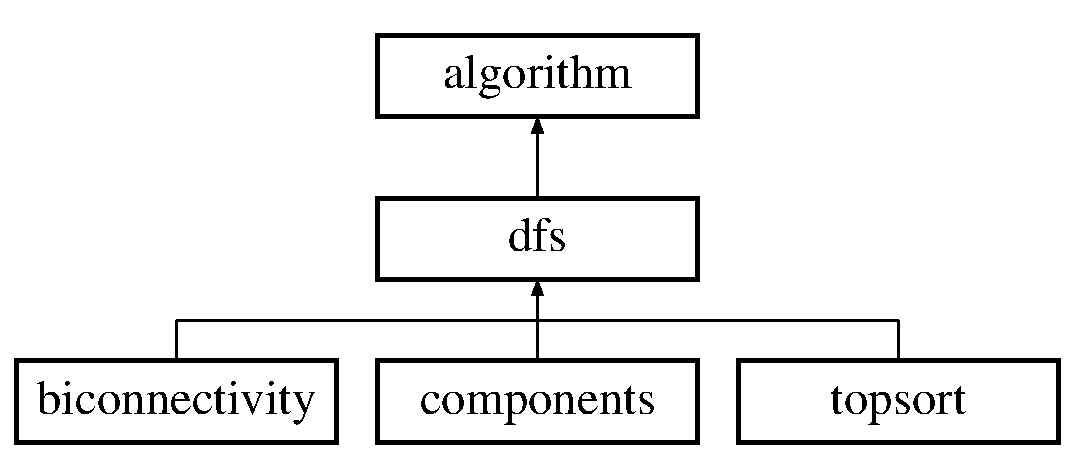
\includegraphics[height=3.000000cm]{classdfs}
\end{center}
\end{figure}
\subsection*{Public Types}
\begin{DoxyCompactItemize}
\item 
\mbox{\Hypertarget{classdfs_a0eee0ddec5343c05f617d6d7aabb6d19}\label{classdfs_a0eee0ddec5343c05f617d6d7aabb6d19}} 
typedef list$<$ \mbox{\hyperlink{classedge}{edge}} $>$\+::const\+\_\+iterator \mbox{\hyperlink{classdfs_a0eee0ddec5343c05f617d6d7aabb6d19}{tree\+\_\+edges\+\_\+iterator}}
\begin{DoxyCompactList}\small\item\em Iterator for the tree edges of the D\+F\+S-\/tree. \end{DoxyCompactList}\item 
\mbox{\Hypertarget{classdfs_ad040ddae37492e18c8e029406d667bd9}\label{classdfs_ad040ddae37492e18c8e029406d667bd9}} 
typedef list$<$ \mbox{\hyperlink{classnode}{node}} $>$\+::const\+\_\+iterator \mbox{\hyperlink{classdfs_ad040ddae37492e18c8e029406d667bd9}{dfs\+\_\+iterator}}
\begin{DoxyCompactList}\small\item\em Iterator for the (reached) nodes in D\+F\+S-\/order. \end{DoxyCompactList}\item 
\mbox{\Hypertarget{classdfs_ae7301f3d4417e60fb3a499180375194e}\label{classdfs_ae7301f3d4417e60fb3a499180375194e}} 
typedef list$<$ \mbox{\hyperlink{classedge}{edge}} $>$\+::const\+\_\+iterator \mbox{\hyperlink{classdfs_ae7301f3d4417e60fb3a499180375194e}{non\+\_\+tree\+\_\+edges\+\_\+iterator}}
\begin{DoxyCompactList}\small\item\em Iterator for the non-\/tree-\/edges. \end{DoxyCompactList}\item 
\mbox{\Hypertarget{classdfs_a17cb59c8a1fead11fa6b0c85cf5a478e}\label{classdfs_a17cb59c8a1fead11fa6b0c85cf5a478e}} 
typedef list$<$ \mbox{\hyperlink{classdfs_ad040ddae37492e18c8e029406d667bd9}{dfs\+\_\+iterator}} $>$\+::const\+\_\+iterator \mbox{\hyperlink{classdfs_a17cb59c8a1fead11fa6b0c85cf5a478e}{roots\+\_\+iterator}}
\begin{DoxyCompactList}\small\item\em Iterator for the roots of the D\+F\+S-\/forest. \end{DoxyCompactList}\end{DoxyCompactItemize}
\subsection*{Public Member Functions}
\begin{DoxyCompactItemize}
\item 
\mbox{\Hypertarget{classdfs_a5232bc41ab202b6278a84bd97c803a0d}\label{classdfs_a5232bc41ab202b6278a84bd97c803a0d}} 
\mbox{\hyperlink{classdfs_a5232bc41ab202b6278a84bd97c803a0d}{dfs}} ()
\begin{DoxyCompactList}\small\item\em Constructor. \end{DoxyCompactList}\item 
\mbox{\Hypertarget{classdfs_aff2e95c12935221a94551393f7e36c6e}\label{classdfs_aff2e95c12935221a94551393f7e36c6e}} 
virtual \mbox{\hyperlink{classdfs_aff2e95c12935221a94551393f7e36c6e}{$\sim$dfs}} ()
\begin{DoxyCompactList}\small\item\em Destructor. \end{DoxyCompactList}\item 
int \mbox{\hyperlink{classdfs_af0863b8974d5fd58cd0375c78ed8163b}{run}} (\mbox{\hyperlink{classgraph}{graph}} \&G)
\begin{DoxyCompactList}\small\item\em Applies algorithm to graph g. \end{DoxyCompactList}\item 
virtual int \mbox{\hyperlink{classdfs_a1af70060897529e67910f589b047e576}{check}} (\mbox{\hyperlink{classgraph}{graph}} \&G)
\begin{DoxyCompactList}\small\item\em Checks whether the preconditions for D\+FS are satisfied. \end{DoxyCompactList}\item 
virtual void \mbox{\hyperlink{classdfs_affaffda8be8418d6dbf396c5b1d6b81a}{reset}} ()
\begin{DoxyCompactList}\small\item\em Resets algorithm. \end{DoxyCompactList}\item 
void \mbox{\hyperlink{classdfs_aad21fd0d3036350fd341f877d5747852}{start\+\_\+node}} (const \mbox{\hyperlink{classnode}{node}} \&n)
\begin{DoxyCompactList}\small\item\em Sets start-\/node for D\+FS. \end{DoxyCompactList}\item 
\mbox{\hyperlink{classnode}{node}} \mbox{\hyperlink{classdfs_a7688d8eaf1308438820fec2ffe21257c}{start\+\_\+node}} () const
\begin{DoxyCompactList}\small\item\em Returns start-\/node for D\+FS. \end{DoxyCompactList}\item 
void \mbox{\hyperlink{classdfs_aa7c864a6f3a120720138b187b3ed95b5}{scan\+\_\+whole\+\_\+graph}} (bool set)
\begin{DoxyCompactList}\small\item\em Enables or disables scanning of the whole graph. \end{DoxyCompactList}\item 
bool \mbox{\hyperlink{classdfs_a025ed2d6101a7b9f72578a52b484ef50}{scan\+\_\+whole\+\_\+graph}} () const
\begin{DoxyCompactList}\small\item\em Returns true iff the whole graph will be scanned. \end{DoxyCompactList}\item 
void \mbox{\hyperlink{classdfs_a70862ea715c52eb95fb704afd3a6e676}{calc\+\_\+comp\+\_\+num}} (bool set)
\begin{DoxyCompactList}\small\item\em Enables or Disables the calculation of the completion number. \end{DoxyCompactList}\item 
bool \mbox{\hyperlink{classdfs_aba80ac24a78448f10b32473633cd2a5d}{calc\+\_\+comp\+\_\+num}} () const
\begin{DoxyCompactList}\small\item\em Returns true iff completion-\/numbers will be calculated. \end{DoxyCompactList}\item 
void \mbox{\hyperlink{classdfs_a7043f46eb3887cbcbb1391fc783407a4}{store\+\_\+preds}} (bool set)
\begin{DoxyCompactList}\small\item\em Enables or disables the storing of predecessors. \end{DoxyCompactList}\item 
bool \mbox{\hyperlink{classdfs_ad0233128f2958d630102096aa6f3b9ef}{store\+\_\+preds}} () const
\begin{DoxyCompactList}\small\item\em Returns true iff the storing of predecessors is enabled. \end{DoxyCompactList}\item 
void \mbox{\hyperlink{classdfs_a6f54f1c4339eacc8961e795439d4593d}{store\+\_\+non\+\_\+tree\+\_\+edges}} (bool set)
\begin{DoxyCompactList}\small\item\em Enables the storing of back-\/edges. \end{DoxyCompactList}\item 
bool \mbox{\hyperlink{classdfs_a6ac1f01ff594fbbc6e8d6b5bd03fc9ab}{store\+\_\+non\+\_\+tree\+\_\+edges}} () const
\begin{DoxyCompactList}\small\item\em Returns true iff the storing of non-\/tree-\/edges is enabled. \end{DoxyCompactList}\item 
bool \mbox{\hyperlink{classdfs_a2948061eb1ea02f57614f9044c8e63cf}{reached}} (const \mbox{\hyperlink{classnode}{node}} \&n) const
\begin{DoxyCompactList}\small\item\em Checks whether node {\itshape n} was reached in last D\+FS. \end{DoxyCompactList}\item 
int \mbox{\hyperlink{classdfs_a315f16831a0bd333960e87e045cb37c8}{dfs\+\_\+num}} (const \mbox{\hyperlink{classnode}{node}} \&n) const
\begin{DoxyCompactList}\small\item\em D\+F\+S-\/\+Number of {\itshape n}. \end{DoxyCompactList}\item 
int \mbox{\hyperlink{classdfs_a014b90894a47fa5abb7f4e5030be2c3e}{operator\mbox{[}$\,$\mbox{]}}} (const \mbox{\hyperlink{classnode}{node}} \&n) const
\begin{DoxyCompactList}\small\item\em D\+F\+S-\/\+Number of {\itshape n}. \end{DoxyCompactList}\item 
int \mbox{\hyperlink{classdfs_aceb066c806cb0beb5688b167a17387c7}{comp\+\_\+num}} (const \mbox{\hyperlink{classnode}{node}} \&n) const
\begin{DoxyCompactList}\small\item\em Completion-\/number of node {\itshape n}, if enabled in last run. \end{DoxyCompactList}\item 
\mbox{\hyperlink{classnode}{node}} \mbox{\hyperlink{classdfs_a3012717ce541b3e56943e2c2c50efdf6}{father}} (const \mbox{\hyperlink{classnode}{node}} \&n) const
\begin{DoxyCompactList}\small\item\em Returns father of node {\itshape n} in D\+F\+S-\/forest. \end{DoxyCompactList}\item 
\mbox{\hyperlink{classdfs_a0eee0ddec5343c05f617d6d7aabb6d19}{tree\+\_\+edges\+\_\+iterator}} \mbox{\hyperlink{classdfs_afe193938a05b114870c19163731273c8}{tree\+\_\+edges\+\_\+begin}} () const
\begin{DoxyCompactList}\small\item\em Iterate through all edges picked in last D\+FS. \end{DoxyCompactList}\item 
\mbox{\hyperlink{classdfs_a0eee0ddec5343c05f617d6d7aabb6d19}{tree\+\_\+edges\+\_\+iterator}} \mbox{\hyperlink{classdfs_ad1b9f759569cb52ba7ee415862c79831}{tree\+\_\+edges\+\_\+end}} () const
\begin{DoxyCompactList}\small\item\em End-\/iterator for iteration through all edges picked in last D\+FS. \end{DoxyCompactList}\item 
\mbox{\hyperlink{classdfs_ad040ddae37492e18c8e029406d667bd9}{dfs\+\_\+iterator}} \mbox{\hyperlink{classdfs_ab06650dd8cbd5e76b0c73b71458ec5ec}{begin}} () const
\begin{DoxyCompactList}\small\item\em Iterate through all (reached) nodes in D\+F\+S-\/order. \end{DoxyCompactList}\item 
\mbox{\hyperlink{classdfs_ad040ddae37492e18c8e029406d667bd9}{dfs\+\_\+iterator}} \mbox{\hyperlink{classdfs_af847633fa642258d3522e8deb26aef37}{end}} () const
\begin{DoxyCompactList}\small\item\em End-\/\+Iterator for iteration through all (reached) nodes in D\+F\+S-\/order. \end{DoxyCompactList}\item 
\mbox{\hyperlink{classdfs_ae7301f3d4417e60fb3a499180375194e}{non\+\_\+tree\+\_\+edges\+\_\+iterator}} \mbox{\hyperlink{classdfs_a4efe5bb72d00305e6b226e67c2b2ef6e}{non\+\_\+tree\+\_\+edges\+\_\+begin}} () const
\begin{DoxyCompactList}\small\item\em Iterate through all non-\/tree-\/edges (if enabled). \end{DoxyCompactList}\item 
\mbox{\hyperlink{classdfs_ae7301f3d4417e60fb3a499180375194e}{non\+\_\+tree\+\_\+edges\+\_\+iterator}} \mbox{\hyperlink{classdfs_ad9cd92a18bda23edca8ab3ac60a15ef4}{non\+\_\+tree\+\_\+edges\+\_\+end}} () const
\begin{DoxyCompactList}\small\item\em End-\/iterator for iteration through all non-\/tree-\/edges (if enabled). \end{DoxyCompactList}\item 
\mbox{\hyperlink{classdfs_a17cb59c8a1fead11fa6b0c85cf5a478e}{roots\+\_\+iterator}} \mbox{\hyperlink{classdfs_af56fa2b736f0b924dba1257e18ba4b61}{roots\+\_\+begin}} () const
\begin{DoxyCompactList}\small\item\em Iterator pointing towards the first root in the D\+F\+S-\/forest. \end{DoxyCompactList}\item 
\mbox{\hyperlink{classdfs_a17cb59c8a1fead11fa6b0c85cf5a478e}{roots\+\_\+iterator}} \mbox{\hyperlink{classdfs_ae1a61d8c2d8d99059cab410f766ec73f}{roots\+\_\+end}} () const
\begin{DoxyCompactList}\small\item\em Iterator pointing to the end of all roots. \end{DoxyCompactList}\item 
int \mbox{\hyperlink{classdfs_ae8849a552721ad4af5d9a81c6da35822}{number\+\_\+of\+\_\+reached\+\_\+nodes}} () const
\begin{DoxyCompactList}\small\item\em Number of nodes reached in last D\+FS. \end{DoxyCompactList}\item 
virtual void \mbox{\hyperlink{classdfs_acc82574cd42ab8256e685374bee5fabb}{init\+\_\+handler}} (\mbox{\hyperlink{classgraph}{graph}} \&G)
\begin{DoxyCompactList}\small\item\em Handler called before the start of D\+FS. \end{DoxyCompactList}\item 
virtual void \mbox{\hyperlink{classdfs_ab96c7c6183856dd9e356fdcf50835b32}{end\+\_\+handler}} (\mbox{\hyperlink{classgraph}{graph}} \&G)
\begin{DoxyCompactList}\small\item\em Handler called at the end of D\+FS. \end{DoxyCompactList}\item 
virtual void \mbox{\hyperlink{classdfs_a73dabe5882226b53494a487b7c34f1d1}{entry\+\_\+handler}} (\mbox{\hyperlink{classgraph}{graph}} \&G, \mbox{\hyperlink{classnode}{node}} \&n, \mbox{\hyperlink{classnode}{node}} \&f)
\begin{DoxyCompactList}\small\item\em Handler called when touching node {\itshape n}. \end{DoxyCompactList}\item 
virtual void \mbox{\hyperlink{classdfs_a8071fc4e82deff7ceb2790cd4eb42280}{leave\+\_\+handler}} (\mbox{\hyperlink{classgraph}{graph}} \&G, \mbox{\hyperlink{classnode}{node}} \&n, \mbox{\hyperlink{classnode}{node}} \&f)
\begin{DoxyCompactList}\small\item\em Handler called after all the adjacent edges of {\itshape n} have been examined. \end{DoxyCompactList}\item 
virtual void \mbox{\hyperlink{classdfs_ae3f095c9fe6106e82c24543da4844ea3}{before\+\_\+recursive\+\_\+call\+\_\+handler}} (\mbox{\hyperlink{classgraph}{graph}} \&G, \mbox{\hyperlink{classedge}{edge}} \&e, \mbox{\hyperlink{classnode}{node}} \&n)
\begin{DoxyCompactList}\small\item\em Handler called when a unused node {\itshape n} connected to the actual node by {\itshape e} is found. \end{DoxyCompactList}\item 
virtual void \mbox{\hyperlink{classdfs_a25ae75fe08f1d8c0fedcf9dcae09d092}{after\+\_\+recursive\+\_\+call\+\_\+handler}} (\mbox{\hyperlink{classgraph}{graph}} \&G, \mbox{\hyperlink{classedge}{edge}} \&e, \mbox{\hyperlink{classnode}{node}} \&n)
\begin{DoxyCompactList}\small\item\em Handler called after the algorithm returns from the subtree starting at {\itshape n} connected to the actual node by {\itshape e}. \end{DoxyCompactList}\item 
virtual void \mbox{\hyperlink{classdfs_adf1c667188e632761c63f529537c544c}{old\+\_\+adj\+\_\+node\+\_\+handler}} (\mbox{\hyperlink{classgraph}{graph}} \&G, \mbox{\hyperlink{classedge}{edge}} \&e, \mbox{\hyperlink{classnode}{node}} \&n)
\begin{DoxyCompactList}\small\item\em Handler called when a already marked node {\itshape n} connected to the actual node by {\itshape e} is found during the search of all adjacent edges of the actual node. \end{DoxyCompactList}\item 
virtual void \mbox{\hyperlink{classdfs_a3b5fbea7a7baed9946cfb4444a7f20ea}{new\+\_\+start\+\_\+handler}} (\mbox{\hyperlink{classgraph}{graph}} \&G, \mbox{\hyperlink{classnode}{node}} \&n)
\begin{DoxyCompactList}\small\item\em Called when D\+FS is started with start-\/node {\itshape n}. \end{DoxyCompactList}\end{DoxyCompactItemize}
\subsection*{Protected Attributes}
\begin{DoxyCompactItemize}
\item 
\mbox{\Hypertarget{classdfs_aedaf2b485ff83150b1de6c305922473b}\label{classdfs_aedaf2b485ff83150b1de6c305922473b}} 
int {\bfseries act\+\_\+dfs\+\_\+num}
\item 
\mbox{\Hypertarget{classdfs_ab0251ac30adfd569e214a64db7f3a905}\label{classdfs_ab0251ac30adfd569e214a64db7f3a905}} 
int {\bfseries act\+\_\+comp\+\_\+num}
\item 
\mbox{\Hypertarget{classdfs_ac1f76ebbcb2489fb6456abf6791aa2f2}\label{classdfs_ac1f76ebbcb2489fb6456abf6791aa2f2}} 
list$<$ \mbox{\hyperlink{classedge}{edge}} $>$ {\bfseries tree}
\item 
\mbox{\Hypertarget{classdfs_a7654d7b912b2c66cc5c483774e224803}\label{classdfs_a7654d7b912b2c66cc5c483774e224803}} 
list$<$ \mbox{\hyperlink{classnode}{node}} $>$ {\bfseries dfs\+\_\+order}
\item 
\mbox{\Hypertarget{classdfs_a99727f2274d6af63daae4f0518f3adbe}\label{classdfs_a99727f2274d6af63daae4f0518f3adbe}} 
\mbox{\hyperlink{classnode__map}{node\+\_\+map}}$<$ int $>$ {\bfseries dfs\+\_\+number}
\item 
\mbox{\Hypertarget{classdfs_acb11186a1a2a2a1f38cdc0674340ba37}\label{classdfs_acb11186a1a2a2a1f38cdc0674340ba37}} 
int {\bfseries reached\+\_\+nodes}
\item 
\mbox{\Hypertarget{classdfs_afc18288747491be301d6d8d85d8f220b}\label{classdfs_afc18288747491be301d6d8d85d8f220b}} 
\mbox{\hyperlink{classedge__map}{edge\+\_\+map}}$<$ int $>$ $\ast$ {\bfseries used}
\item 
\mbox{\Hypertarget{classdfs_a85b090809ab552355cbb2722558eccd4}\label{classdfs_a85b090809ab552355cbb2722558eccd4}} 
list$<$ \mbox{\hyperlink{classdfs_ad040ddae37492e18c8e029406d667bd9}{dfs\+\_\+iterator}} $>$ {\bfseries roots}
\item 
\mbox{\Hypertarget{classdfs_a00db016ac7eab69045cae408008890c1}\label{classdfs_a00db016ac7eab69045cae408008890c1}} 
\mbox{\hyperlink{classnode__map}{node\+\_\+map}}$<$ int $>$ $\ast$ {\bfseries comp\+\_\+number}
\item 
\mbox{\Hypertarget{classdfs_a3fdeb5a211a1bc1753b2a637258c5355}\label{classdfs_a3fdeb5a211a1bc1753b2a637258c5355}} 
\mbox{\hyperlink{classnode__map}{node\+\_\+map}}$<$ \mbox{\hyperlink{classnode}{node}} $>$ $\ast$ {\bfseries preds}
\item 
\mbox{\Hypertarget{classdfs_a109335d8c9e025a427177b30e25a18d5}\label{classdfs_a109335d8c9e025a427177b30e25a18d5}} 
list$<$ \mbox{\hyperlink{classedge}{edge}} $>$ $\ast$ {\bfseries back\+\_\+edges}
\item 
\mbox{\Hypertarget{classdfs_af677cfc31fe06a18dd3a3aae7f7d112b}\label{classdfs_af677cfc31fe06a18dd3a3aae7f7d112b}} 
\mbox{\hyperlink{classnode}{node}} {\bfseries start}
\item 
\mbox{\Hypertarget{classdfs_ab8342c80ab208ef0e0d781f0769d0d95}\label{classdfs_ab8342c80ab208ef0e0d781f0769d0d95}} 
bool {\bfseries whole\+\_\+graph}
\end{DoxyCompactItemize}


\subsection{Detailed Description}
Depth-\/\+First-\/\+Search (D\+FS) algorithm. 

\begin{DoxyParagraph}{Date}
2019/05/07 15\+:58\+:54 
\end{DoxyParagraph}
\begin{DoxyParagraph}{Revision}
1.\+25 
\end{DoxyParagraph}


Encapsulates the D\+FS algoritm together with all the data produced by a run of D\+FS. Since there exits so much different things which one might want to calculate during a D\+FS this class provides basically two different customization features. First it is possible to take influence on the behaviour of this algortihm by changing some of the following options\+:
\begin{DoxyItemize}
\item \mbox{\hyperlink{classdfs_aad21fd0d3036350fd341f877d5747852}{dfs\+::start\+\_\+node}} (default\+: an arbitrary node will be chosen)
\item \mbox{\hyperlink{classdfs_aa7c864a6f3a120720138b187b3ed95b5}{dfs\+::scan\+\_\+whole\+\_\+graph}} states whether B\+FS will be continued in the unused part of the graph, if not all nodes were touched at the end of D\+FS started at the start-\/node. (default\+: disabled)
\item \mbox{\hyperlink{classdfs_a70862ea715c52eb95fb704afd3a6e676}{dfs\+::calc\+\_\+comp\+\_\+num}} toggle storing of completion-\/numbers for each node, i.\+e. a numbering which reflects the order in which nodes were {\itshape finished}. (default\+: disabled)
\item \mbox{\hyperlink{classdfs_a7043f46eb3887cbcbb1391fc783407a4}{dfs\+::store\+\_\+preds}} toggle storing the predecessor of each node, i.\+e. the father in D\+F\+S-\/tree. (default\+: disabled)
\item \mbox{\hyperlink{classdfs_a6f54f1c4339eacc8961e795439d4593d}{dfs\+::store\+\_\+non\+\_\+tree\+\_\+edges}} toggle storing of all non-\/tree-\/edges (tree-\/edges are always stored) in a list and thus enable or disable iteration through all non-\/tree-\/edges. (default\+: disabled)
\end{DoxyItemize}

But the trouble with most D\+F\+S-\/algorithm is that one always wants to add a little bit of code somewhere in the algorithm. And then there are only two ways to get this done. The more efficient one (in terms of runtime) is to implement the D\+FS anew and add the new code where necessary. The other way (which is more efficient in terms of code-\/writing) is to take the algorithm as provided and run through the list of nodes it returns (resulting in an extra factor of 2).

Our D\+F\+S-\/algoritm class provides a new method to add small pieces of code to the algorithm\+: Handler. These are virtual functions called at well-\/defined, important states of the algorithm (e.\+g. before a new recursive call). So the only thing to do is to derive your extended D\+FS from this class and to override the handlers where needed. In detail there are the following handler supported (have a look at the source code for details)\+:
\begin{DoxyItemize}
\item \mbox{\hyperlink{classdfs_acc82574cd42ab8256e685374bee5fabb}{dfs\+::init\+\_\+handler}}
\item \mbox{\hyperlink{classdfs_ab96c7c6183856dd9e356fdcf50835b32}{dfs\+::end\+\_\+handler}}
\item \mbox{\hyperlink{classdfs_a73dabe5882226b53494a487b7c34f1d1}{dfs\+::entry\+\_\+handler}}
\item \mbox{\hyperlink{classdfs_a8071fc4e82deff7ceb2790cd4eb42280}{dfs\+::leave\+\_\+handler}}
\item \mbox{\hyperlink{classdfs_ae3f095c9fe6106e82c24543da4844ea3}{dfs\+::before\+\_\+recursive\+\_\+call\+\_\+handler}}
\item \mbox{\hyperlink{classdfs_a25ae75fe08f1d8c0fedcf9dcae09d092}{dfs\+::after\+\_\+recursive\+\_\+call\+\_\+handler}}
\item \mbox{\hyperlink{classdfs_adf1c667188e632761c63f529537c544c}{dfs\+::old\+\_\+adj\+\_\+node\+\_\+handler}}
\item \mbox{\hyperlink{classdfs_a3b5fbea7a7baed9946cfb4444a7f20ea}{dfs\+::new\+\_\+start\+\_\+handler}}
\end{DoxyItemize}

{\itshape Please} {\itshape note\+:} We do {\itshape not} claim that this set of handlers is sufficient in any way. So if you believe that some new handler is needed urgently please let us know.

There is a lot of information stored during D\+FS (e.\+g. nodes in dfs-\/order, list of non-\/tree-\/edges). Some of it can be obtained directly by using the corresponding member-\/function (e.\+g. \mbox{\hyperlink{classdfs_a315f16831a0bd333960e87e045cb37c8}{dfs\+::dfs\+\_\+num}}), but all information that can be thought of as a list (e.\+g. nodes in dfs-\/order) can be accessed through iterators. In detail these are (of course depending on what options are chosen!)\+:
\begin{DoxyItemize}
\item \mbox{\hyperlink{classdfs_ad040ddae37492e18c8e029406d667bd9}{dfs\+::dfs\+\_\+iterator}}
\item \mbox{\hyperlink{classdfs_a0eee0ddec5343c05f617d6d7aabb6d19}{dfs\+::tree\+\_\+edges\+\_\+iterator}}
\item \mbox{\hyperlink{classdfs_ae7301f3d4417e60fb3a499180375194e}{dfs\+::non\+\_\+tree\+\_\+edges\+\_\+iterator}}
\item \mbox{\hyperlink{classdfs_a17cb59c8a1fead11fa6b0c85cf5a478e}{dfs\+::roots\+\_\+iterator}} 
\end{DoxyItemize}

\subsection{Member Function Documentation}
\mbox{\Hypertarget{classdfs_a25ae75fe08f1d8c0fedcf9dcae09d092}\label{classdfs_a25ae75fe08f1d8c0fedcf9dcae09d092}} 
\index{dfs@{dfs}!after\+\_\+recursive\+\_\+call\+\_\+handler@{after\+\_\+recursive\+\_\+call\+\_\+handler}}
\index{after\+\_\+recursive\+\_\+call\+\_\+handler@{after\+\_\+recursive\+\_\+call\+\_\+handler}!dfs@{dfs}}
\subsubsection{\texorpdfstring{after\+\_\+recursive\+\_\+call\+\_\+handler()}{after\_recursive\_call\_handler()}}
{\footnotesize\ttfamily virtual void dfs\+::after\+\_\+recursive\+\_\+call\+\_\+handler (\begin{DoxyParamCaption}\item[{\mbox{\hyperlink{classgraph}{graph}} \&}]{G,  }\item[{\mbox{\hyperlink{classedge}{edge}} \&}]{e,  }\item[{\mbox{\hyperlink{classnode}{node}} \&}]{n }\end{DoxyParamCaption})\hspace{0.3cm}{\ttfamily [inline]}, {\ttfamily [virtual]}}



Handler called after the algorithm returns from the subtree starting at {\itshape n} connected to the actual node by {\itshape e}. 


\begin{DoxyParams}{Parameters}
{\em G} & graph for which D\+FS was invoked. \\
\hline
{\em e} & edge connecting the actual node to the unused one. \\
\hline
{\em n} & unused node. \\
\hline
\end{DoxyParams}


Reimplemented in \mbox{\hyperlink{classbiconnectivity_a69ca91409485b57c486b188596080d7a}{biconnectivity}}.

\mbox{\Hypertarget{classdfs_ae3f095c9fe6106e82c24543da4844ea3}\label{classdfs_ae3f095c9fe6106e82c24543da4844ea3}} 
\index{dfs@{dfs}!before\+\_\+recursive\+\_\+call\+\_\+handler@{before\+\_\+recursive\+\_\+call\+\_\+handler}}
\index{before\+\_\+recursive\+\_\+call\+\_\+handler@{before\+\_\+recursive\+\_\+call\+\_\+handler}!dfs@{dfs}}
\subsubsection{\texorpdfstring{before\+\_\+recursive\+\_\+call\+\_\+handler()}{before\_recursive\_call\_handler()}}
{\footnotesize\ttfamily virtual void dfs\+::before\+\_\+recursive\+\_\+call\+\_\+handler (\begin{DoxyParamCaption}\item[{\mbox{\hyperlink{classgraph}{graph}} \&}]{G,  }\item[{\mbox{\hyperlink{classedge}{edge}} \&}]{e,  }\item[{\mbox{\hyperlink{classnode}{node}} \&}]{n }\end{DoxyParamCaption})\hspace{0.3cm}{\ttfamily [inline]}, {\ttfamily [virtual]}}



Handler called when a unused node {\itshape n} connected to the actual node by {\itshape e} is found. 


\begin{DoxyParams}{Parameters}
{\em G} & graph for which D\+FS was invoked. \\
\hline
{\em e} & edge connecting the actual node to the unused one. \\
\hline
{\em n} & unused node. \\
\hline
\end{DoxyParams}


Reimplemented in \mbox{\hyperlink{classbiconnectivity_a19261e91eef3f7d6b8586fa1eae9f277}{biconnectivity}}, and \mbox{\hyperlink{classcomponents_a587a9c44a80deb4260ccd0728bfeab0f}{components}}.

\mbox{\Hypertarget{classdfs_ab06650dd8cbd5e76b0c73b71458ec5ec}\label{classdfs_ab06650dd8cbd5e76b0c73b71458ec5ec}} 
\index{dfs@{dfs}!begin@{begin}}
\index{begin@{begin}!dfs@{dfs}}
\subsubsection{\texorpdfstring{begin()}{begin()}}
{\footnotesize\ttfamily \mbox{\hyperlink{classdfs_ad040ddae37492e18c8e029406d667bd9}{dfs\+\_\+iterator}} dfs\+::begin (\begin{DoxyParamCaption}{ }\end{DoxyParamCaption}) const\hspace{0.3cm}{\ttfamily [inline]}}



Iterate through all (reached) nodes in D\+F\+S-\/order. 

\begin{DoxyReturn}{Returns}
start for iteration through all nodes in D\+F\+S-\/order. 
\end{DoxyReturn}
\mbox{\Hypertarget{classdfs_a70862ea715c52eb95fb704afd3a6e676}\label{classdfs_a70862ea715c52eb95fb704afd3a6e676}} 
\index{dfs@{dfs}!calc\+\_\+comp\+\_\+num@{calc\+\_\+comp\+\_\+num}}
\index{calc\+\_\+comp\+\_\+num@{calc\+\_\+comp\+\_\+num}!dfs@{dfs}}
\subsubsection{\texorpdfstring{calc\+\_\+comp\+\_\+num()}{calc\_comp\_num()}\hspace{0.1cm}{\footnotesize\ttfamily [1/2]}}
{\footnotesize\ttfamily void dfs\+::calc\+\_\+comp\+\_\+num (\begin{DoxyParamCaption}\item[{bool}]{set }\end{DoxyParamCaption})}



Enables or Disables the calculation of the completion number. 


\begin{DoxyParams}{Parameters}
{\em set} & if true completion-\/numbers will be calculated. \\
\hline
\end{DoxyParams}
\begin{DoxySeeAlso}{See also}
\mbox{\hyperlink{classdfs_aceb066c806cb0beb5688b167a17387c7}{dfs\+::comp\+\_\+num}} 
\end{DoxySeeAlso}
\mbox{\Hypertarget{classdfs_aba80ac24a78448f10b32473633cd2a5d}\label{classdfs_aba80ac24a78448f10b32473633cd2a5d}} 
\index{dfs@{dfs}!calc\+\_\+comp\+\_\+num@{calc\+\_\+comp\+\_\+num}}
\index{calc\+\_\+comp\+\_\+num@{calc\+\_\+comp\+\_\+num}!dfs@{dfs}}
\subsubsection{\texorpdfstring{calc\+\_\+comp\+\_\+num()}{calc\_comp\_num()}\hspace{0.1cm}{\footnotesize\ttfamily [2/2]}}
{\footnotesize\ttfamily bool dfs\+::calc\+\_\+comp\+\_\+num (\begin{DoxyParamCaption}{ }\end{DoxyParamCaption}) const\hspace{0.3cm}{\ttfamily [inline]}}



Returns true iff completion-\/numbers will be calculated. 


\begin{DoxyRetVals}{Return values}
{\em true} & iff completion-\/numbers will be calculated. \\
\hline
\end{DoxyRetVals}
\begin{DoxySeeAlso}{See also}
\mbox{\hyperlink{classdfs_aceb066c806cb0beb5688b167a17387c7}{dfs\+::comp\+\_\+num}} 
\end{DoxySeeAlso}
\mbox{\Hypertarget{classdfs_a1af70060897529e67910f589b047e576}\label{classdfs_a1af70060897529e67910f589b047e576}} 
\index{dfs@{dfs}!check@{check}}
\index{check@{check}!dfs@{dfs}}
\subsubsection{\texorpdfstring{check()}{check()}}
{\footnotesize\ttfamily int dfs\+::check (\begin{DoxyParamCaption}\item[{\mbox{\hyperlink{classgraph}{graph}} \&}]{G }\end{DoxyParamCaption})\hspace{0.3cm}{\ttfamily [virtual]}}



Checks whether the preconditions for D\+FS are satisfied. 

Currently there aren\textquotesingle{}t any restricitions for the D\+FS algorithm.


\begin{DoxyParams}{Parameters}
{\em G} & graph. \\
\hline
\end{DoxyParams}

\begin{DoxyRetVals}{Return values}
{\em \mbox{\hyperlink{classalgorithm_af1a0078e153aa99c24f9bdf0d97f6710aae4c1cd7fe8d8cf4b143241a6e7c31cf}{algorithm\+::\+K\+G\+L\+\_\+\+OK}}} & if algorithm can be applied \\
\hline
{\em \mbox{\hyperlink{classalgorithm_af1a0078e153aa99c24f9bdf0d97f6710ae67bf27b2ef31f73e545a7f9f4a69556}{algorithm\+::\+K\+G\+L\+\_\+\+E\+R\+R\+OR}}} & otherwise. \\
\hline
\end{DoxyRetVals}


Implements \mbox{\hyperlink{classalgorithm_a76361fb03ad1cf643affc51821e43bed}{algorithm}}.



Reimplemented in \mbox{\hyperlink{classtopsort_a777a9a68c4081d22e7b698ed3c515343}{topsort}}, \mbox{\hyperlink{classbiconnectivity_a65e0e821f5e9ce8d210648d462fd2cfa}{biconnectivity}}, and \mbox{\hyperlink{classcomponents_aeeda901d02c65d6c31c8b6148540d7c1}{components}}.

\mbox{\Hypertarget{classdfs_aceb066c806cb0beb5688b167a17387c7}\label{classdfs_aceb066c806cb0beb5688b167a17387c7}} 
\index{dfs@{dfs}!comp\+\_\+num@{comp\+\_\+num}}
\index{comp\+\_\+num@{comp\+\_\+num}!dfs@{dfs}}
\subsubsection{\texorpdfstring{comp\+\_\+num()}{comp\_num()}}
{\footnotesize\ttfamily int dfs\+::comp\+\_\+num (\begin{DoxyParamCaption}\item[{const \mbox{\hyperlink{classnode}{node}} \&}]{n }\end{DoxyParamCaption}) const\hspace{0.3cm}{\ttfamily [inline]}}



Completion-\/number of node {\itshape n}, if enabled in last run. 


\begin{DoxyParams}{Parameters}
{\em n} & node. \\
\hline
\end{DoxyParams}
\begin{DoxyReturn}{Returns}
Completion-\/number of {\itshape n}. 
\end{DoxyReturn}
\begin{DoxySeeAlso}{See also}
\mbox{\hyperlink{classdfs_a70862ea715c52eb95fb704afd3a6e676}{dfs\+::calc\+\_\+comp\+\_\+num}} 
\end{DoxySeeAlso}
\mbox{\Hypertarget{classdfs_a315f16831a0bd333960e87e045cb37c8}\label{classdfs_a315f16831a0bd333960e87e045cb37c8}} 
\index{dfs@{dfs}!dfs\+\_\+num@{dfs\+\_\+num}}
\index{dfs\+\_\+num@{dfs\+\_\+num}!dfs@{dfs}}
\subsubsection{\texorpdfstring{dfs\+\_\+num()}{dfs\_num()}}
{\footnotesize\ttfamily int dfs\+::dfs\+\_\+num (\begin{DoxyParamCaption}\item[{const \mbox{\hyperlink{classnode}{node}} \&}]{n }\end{DoxyParamCaption}) const\hspace{0.3cm}{\ttfamily [inline]}}



D\+F\+S-\/\+Number of {\itshape n}. 

Please note that D\+F\+S-\/\+Number 0 means that this node wasn\textquotesingle{}t reached.


\begin{DoxyParams}{Parameters}
{\em n} & node. \\
\hline
\end{DoxyParams}
\begin{DoxyReturn}{Returns}
D\+F\+S-\/\+Number of {\itshape n}. 
\end{DoxyReturn}
\mbox{\Hypertarget{classdfs_af847633fa642258d3522e8deb26aef37}\label{classdfs_af847633fa642258d3522e8deb26aef37}} 
\index{dfs@{dfs}!end@{end}}
\index{end@{end}!dfs@{dfs}}
\subsubsection{\texorpdfstring{end()}{end()}}
{\footnotesize\ttfamily \mbox{\hyperlink{classdfs_ad040ddae37492e18c8e029406d667bd9}{dfs\+\_\+iterator}} dfs\+::end (\begin{DoxyParamCaption}{ }\end{DoxyParamCaption}) const\hspace{0.3cm}{\ttfamily [inline]}}



End-\/\+Iterator for iteration through all (reached) nodes in D\+F\+S-\/order. 

\begin{DoxyReturn}{Returns}
end for iteration through all (reached) nodes 
\end{DoxyReturn}
\mbox{\Hypertarget{classdfs_ab96c7c6183856dd9e356fdcf50835b32}\label{classdfs_ab96c7c6183856dd9e356fdcf50835b32}} 
\index{dfs@{dfs}!end\+\_\+handler@{end\+\_\+handler}}
\index{end\+\_\+handler@{end\+\_\+handler}!dfs@{dfs}}
\subsubsection{\texorpdfstring{end\+\_\+handler()}{end\_handler()}}
{\footnotesize\ttfamily virtual void dfs\+::end\+\_\+handler (\begin{DoxyParamCaption}\item[{\mbox{\hyperlink{classgraph}{graph}} \&}]{G }\end{DoxyParamCaption})\hspace{0.3cm}{\ttfamily [inline]}, {\ttfamily [virtual]}}



Handler called at the end of D\+FS. 


\begin{DoxyParams}{Parameters}
{\em G} & graph for which D\+FS was invoked. \\
\hline
\end{DoxyParams}


Reimplemented in \mbox{\hyperlink{classbiconnectivity_a2583331a4561f3db221ab674d2e5d75e}{biconnectivity}}.

\mbox{\Hypertarget{classdfs_a73dabe5882226b53494a487b7c34f1d1}\label{classdfs_a73dabe5882226b53494a487b7c34f1d1}} 
\index{dfs@{dfs}!entry\+\_\+handler@{entry\+\_\+handler}}
\index{entry\+\_\+handler@{entry\+\_\+handler}!dfs@{dfs}}
\subsubsection{\texorpdfstring{entry\+\_\+handler()}{entry\_handler()}}
{\footnotesize\ttfamily virtual void dfs\+::entry\+\_\+handler (\begin{DoxyParamCaption}\item[{\mbox{\hyperlink{classgraph}{graph}} \&}]{G,  }\item[{\mbox{\hyperlink{classnode}{node}} \&}]{n,  }\item[{\mbox{\hyperlink{classnode}{node}} \&}]{f }\end{DoxyParamCaption})\hspace{0.3cm}{\ttfamily [inline]}, {\ttfamily [virtual]}}



Handler called when touching node {\itshape n}. 


\begin{DoxyParams}{Parameters}
{\em G} & graph for which D\+FS was invoked. \\
\hline
{\em n} & actual node. \\
\hline
{\em f} & predecessor. \\
\hline
\end{DoxyParams}


Reimplemented in \mbox{\hyperlink{classbiconnectivity_acb402f2d144f84429b3cd009121245b0}{biconnectivity}}.

\mbox{\Hypertarget{classdfs_a3012717ce541b3e56943e2c2c50efdf6}\label{classdfs_a3012717ce541b3e56943e2c2c50efdf6}} 
\index{dfs@{dfs}!father@{father}}
\index{father@{father}!dfs@{dfs}}
\subsubsection{\texorpdfstring{father()}{father()}}
{\footnotesize\ttfamily \mbox{\hyperlink{classnode}{node}} dfs\+::father (\begin{DoxyParamCaption}\item[{const \mbox{\hyperlink{classnode}{node}} \&}]{n }\end{DoxyParamCaption}) const\hspace{0.3cm}{\ttfamily [inline]}}



Returns father of node {\itshape n} in D\+F\+S-\/forest. 

If {\itshape n} is a root in the forest or wasn\textquotesingle{}t reached the return value is {\ttfamily \mbox{\hyperlink{classnode}{node()}}}.


\begin{DoxyParams}{Parameters}
{\em n} & node. \\
\hline
\end{DoxyParams}
\begin{DoxyReturn}{Returns}
Father of {\itshape n}. 
\end{DoxyReturn}
\begin{DoxySeeAlso}{See also}
\mbox{\hyperlink{classdfs_a7043f46eb3887cbcbb1391fc783407a4}{dfs\+::store\+\_\+preds}} 
\end{DoxySeeAlso}
\mbox{\Hypertarget{classdfs_acc82574cd42ab8256e685374bee5fabb}\label{classdfs_acc82574cd42ab8256e685374bee5fabb}} 
\index{dfs@{dfs}!init\+\_\+handler@{init\+\_\+handler}}
\index{init\+\_\+handler@{init\+\_\+handler}!dfs@{dfs}}
\subsubsection{\texorpdfstring{init\+\_\+handler()}{init\_handler()}}
{\footnotesize\ttfamily virtual void dfs\+::init\+\_\+handler (\begin{DoxyParamCaption}\item[{\mbox{\hyperlink{classgraph}{graph}} \&}]{G }\end{DoxyParamCaption})\hspace{0.3cm}{\ttfamily [inline]}, {\ttfamily [virtual]}}



Handler called before the start of D\+FS. 


\begin{DoxyParams}{Parameters}
{\em G} & graph for which D\+FS was invoked. \\
\hline
\end{DoxyParams}


Reimplemented in \mbox{\hyperlink{classbiconnectivity_a64adab869e0080e3a1f8479e70010317}{biconnectivity}}, and \mbox{\hyperlink{classtopsort_a21aaf28fc280094ed43288e58d8e3ae1}{topsort}}.

\mbox{\Hypertarget{classdfs_a8071fc4e82deff7ceb2790cd4eb42280}\label{classdfs_a8071fc4e82deff7ceb2790cd4eb42280}} 
\index{dfs@{dfs}!leave\+\_\+handler@{leave\+\_\+handler}}
\index{leave\+\_\+handler@{leave\+\_\+handler}!dfs@{dfs}}
\subsubsection{\texorpdfstring{leave\+\_\+handler()}{leave\_handler()}}
{\footnotesize\ttfamily virtual void dfs\+::leave\+\_\+handler (\begin{DoxyParamCaption}\item[{\mbox{\hyperlink{classgraph}{graph}} \&}]{G,  }\item[{\mbox{\hyperlink{classnode}{node}} \&}]{n,  }\item[{\mbox{\hyperlink{classnode}{node}} \&}]{f }\end{DoxyParamCaption})\hspace{0.3cm}{\ttfamily [inline]}, {\ttfamily [virtual]}}



Handler called after all the adjacent edges of {\itshape n} have been examined. 


\begin{DoxyParams}{Parameters}
{\em G} & graph for which D\+FS was invoked. \\
\hline
{\em n} & actual node. \\
\hline
{\em f} & predecessor. \\
\hline
\end{DoxyParams}


Reimplemented in \mbox{\hyperlink{classbiconnectivity_a868587fdc4dbb3bf80899d1c7d49b558}{biconnectivity}}, and \mbox{\hyperlink{classtopsort_afd27bb676fd3987456bf71d83c05acb8}{topsort}}.

\mbox{\Hypertarget{classdfs_a3b5fbea7a7baed9946cfb4444a7f20ea}\label{classdfs_a3b5fbea7a7baed9946cfb4444a7f20ea}} 
\index{dfs@{dfs}!new\+\_\+start\+\_\+handler@{new\+\_\+start\+\_\+handler}}
\index{new\+\_\+start\+\_\+handler@{new\+\_\+start\+\_\+handler}!dfs@{dfs}}
\subsubsection{\texorpdfstring{new\+\_\+start\+\_\+handler()}{new\_start\_handler()}}
{\footnotesize\ttfamily virtual void dfs\+::new\+\_\+start\+\_\+handler (\begin{DoxyParamCaption}\item[{\mbox{\hyperlink{classgraph}{graph}} \&}]{G,  }\item[{\mbox{\hyperlink{classnode}{node}} \&}]{n }\end{DoxyParamCaption})\hspace{0.3cm}{\ttfamily [inline]}, {\ttfamily [virtual]}}



Called when D\+FS is started with start-\/node {\itshape n}. 

This is particularly useful when D\+FS was invoked with the \mbox{\hyperlink{classdfs_aa7c864a6f3a120720138b187b3ed95b5}{scan\+\_\+whole\+\_\+graph}} option.


\begin{DoxyParams}{Parameters}
{\em G} & graph for which D\+FS was invoked. \\
\hline
{\em n} & start-\/node. \\
\hline
\end{DoxyParams}


Reimplemented in \mbox{\hyperlink{classbiconnectivity_ae94213830755f1f4d477ec6bff0f25b8}{biconnectivity}}, and \mbox{\hyperlink{classcomponents_af53365bd737b34cf63e4a6b10879ffcc}{components}}.

\mbox{\Hypertarget{classdfs_a4efe5bb72d00305e6b226e67c2b2ef6e}\label{classdfs_a4efe5bb72d00305e6b226e67c2b2ef6e}} 
\index{dfs@{dfs}!non\+\_\+tree\+\_\+edges\+\_\+begin@{non\+\_\+tree\+\_\+edges\+\_\+begin}}
\index{non\+\_\+tree\+\_\+edges\+\_\+begin@{non\+\_\+tree\+\_\+edges\+\_\+begin}!dfs@{dfs}}
\subsubsection{\texorpdfstring{non\+\_\+tree\+\_\+edges\+\_\+begin()}{non\_tree\_edges\_begin()}}
{\footnotesize\ttfamily \mbox{\hyperlink{classdfs_ae7301f3d4417e60fb3a499180375194e}{non\+\_\+tree\+\_\+edges\+\_\+iterator}} dfs\+::non\+\_\+tree\+\_\+edges\+\_\+begin (\begin{DoxyParamCaption}{ }\end{DoxyParamCaption}) const\hspace{0.3cm}{\ttfamily [inline]}}



Iterate through all non-\/tree-\/edges (if enabled). 

\begin{DoxyReturn}{Returns}
start for iteration through all non-\/tree-\/edges. 
\end{DoxyReturn}
\begin{DoxySeeAlso}{See also}
\mbox{\hyperlink{classdfs_a6f54f1c4339eacc8961e795439d4593d}{dfs\+::store\+\_\+non\+\_\+tree\+\_\+edges}} 
\end{DoxySeeAlso}
\mbox{\Hypertarget{classdfs_ad9cd92a18bda23edca8ab3ac60a15ef4}\label{classdfs_ad9cd92a18bda23edca8ab3ac60a15ef4}} 
\index{dfs@{dfs}!non\+\_\+tree\+\_\+edges\+\_\+end@{non\+\_\+tree\+\_\+edges\+\_\+end}}
\index{non\+\_\+tree\+\_\+edges\+\_\+end@{non\+\_\+tree\+\_\+edges\+\_\+end}!dfs@{dfs}}
\subsubsection{\texorpdfstring{non\+\_\+tree\+\_\+edges\+\_\+end()}{non\_tree\_edges\_end()}}
{\footnotesize\ttfamily \mbox{\hyperlink{classdfs_ae7301f3d4417e60fb3a499180375194e}{non\+\_\+tree\+\_\+edges\+\_\+iterator}} dfs\+::non\+\_\+tree\+\_\+edges\+\_\+end (\begin{DoxyParamCaption}{ }\end{DoxyParamCaption}) const\hspace{0.3cm}{\ttfamily [inline]}}



End-\/iterator for iteration through all non-\/tree-\/edges (if enabled). 

\begin{DoxyReturn}{Returns}
end for iteration through all non-\/tree-\/edges. 
\end{DoxyReturn}
\begin{DoxySeeAlso}{See also}
\mbox{\hyperlink{classdfs_a6f54f1c4339eacc8961e795439d4593d}{dfs\+::store\+\_\+non\+\_\+tree\+\_\+edges}} 
\end{DoxySeeAlso}
\mbox{\Hypertarget{classdfs_ae8849a552721ad4af5d9a81c6da35822}\label{classdfs_ae8849a552721ad4af5d9a81c6da35822}} 
\index{dfs@{dfs}!number\+\_\+of\+\_\+reached\+\_\+nodes@{number\+\_\+of\+\_\+reached\+\_\+nodes}}
\index{number\+\_\+of\+\_\+reached\+\_\+nodes@{number\+\_\+of\+\_\+reached\+\_\+nodes}!dfs@{dfs}}
\subsubsection{\texorpdfstring{number\+\_\+of\+\_\+reached\+\_\+nodes()}{number\_of\_reached\_nodes()}}
{\footnotesize\ttfamily int dfs\+::number\+\_\+of\+\_\+reached\+\_\+nodes (\begin{DoxyParamCaption}{ }\end{DoxyParamCaption}) const\hspace{0.3cm}{\ttfamily [inline]}}



Number of nodes reached in last D\+FS. 

\begin{DoxyReturn}{Returns}
number of reached nodes. 
\end{DoxyReturn}
\begin{DoxySeeAlso}{See also}
\mbox{\hyperlink{classdfs_aa7c864a6f3a120720138b187b3ed95b5}{dfs\+::scan\+\_\+whole\+\_\+graph}} 
\end{DoxySeeAlso}
\mbox{\Hypertarget{classdfs_adf1c667188e632761c63f529537c544c}\label{classdfs_adf1c667188e632761c63f529537c544c}} 
\index{dfs@{dfs}!old\+\_\+adj\+\_\+node\+\_\+handler@{old\+\_\+adj\+\_\+node\+\_\+handler}}
\index{old\+\_\+adj\+\_\+node\+\_\+handler@{old\+\_\+adj\+\_\+node\+\_\+handler}!dfs@{dfs}}
\subsubsection{\texorpdfstring{old\+\_\+adj\+\_\+node\+\_\+handler()}{old\_adj\_node\_handler()}}
{\footnotesize\ttfamily virtual void dfs\+::old\+\_\+adj\+\_\+node\+\_\+handler (\begin{DoxyParamCaption}\item[{\mbox{\hyperlink{classgraph}{graph}} \&}]{G,  }\item[{\mbox{\hyperlink{classedge}{edge}} \&}]{e,  }\item[{\mbox{\hyperlink{classnode}{node}} \&}]{n }\end{DoxyParamCaption})\hspace{0.3cm}{\ttfamily [inline]}, {\ttfamily [virtual]}}



Handler called when a already marked node {\itshape n} connected to the actual node by {\itshape e} is found during the search of all adjacent edges of the actual node. 


\begin{DoxyParams}{Parameters}
{\em G} & graph for which D\+FS was invoked. \\
\hline
{\em e} & edge connecting the actual node to the old one. \\
\hline
{\em n} & used node. \\
\hline
\end{DoxyParams}


Reimplemented in \mbox{\hyperlink{classbiconnectivity_a92228b87472140374dffea7d9f7ee20d}{biconnectivity}}, \mbox{\hyperlink{classtopsort_ab42587b5a1e776be5106502dfeb6b0b1}{topsort}}, and \mbox{\hyperlink{classcomponents_afcf7a0bee5104bba7986039a9d6bd1ee}{components}}.

\mbox{\Hypertarget{classdfs_a014b90894a47fa5abb7f4e5030be2c3e}\label{classdfs_a014b90894a47fa5abb7f4e5030be2c3e}} 
\index{dfs@{dfs}!operator\mbox{[}\mbox{]}@{operator[]}}
\index{operator\mbox{[}\mbox{]}@{operator[]}!dfs@{dfs}}
\subsubsection{\texorpdfstring{operator[]()}{operator[]()}}
{\footnotesize\ttfamily int dfs\+::operator\mbox{[}$\,$\mbox{]} (\begin{DoxyParamCaption}\item[{const \mbox{\hyperlink{classnode}{node}} \&}]{n }\end{DoxyParamCaption}) const\hspace{0.3cm}{\ttfamily [inline]}}



D\+F\+S-\/\+Number of {\itshape n}. 

Please note that D\+F\+S-\/\+Number 0 means that this node wasn\textquotesingle{}t reached.


\begin{DoxyParams}{Parameters}
{\em n} & node. \\
\hline
\end{DoxyParams}
\begin{DoxyReturn}{Returns}
D\+F\+S-\/\+Number of {\itshape n}. 
\end{DoxyReturn}
\mbox{\Hypertarget{classdfs_a2948061eb1ea02f57614f9044c8e63cf}\label{classdfs_a2948061eb1ea02f57614f9044c8e63cf}} 
\index{dfs@{dfs}!reached@{reached}}
\index{reached@{reached}!dfs@{dfs}}
\subsubsection{\texorpdfstring{reached()}{reached()}}
{\footnotesize\ttfamily bool dfs\+::reached (\begin{DoxyParamCaption}\item[{const \mbox{\hyperlink{classnode}{node}} \&}]{n }\end{DoxyParamCaption}) const\hspace{0.3cm}{\ttfamily [inline]}}



Checks whether node {\itshape n} was reached in last D\+FS. 


\begin{DoxyParams}{Parameters}
{\em n} & node to be checked. \\
\hline
\end{DoxyParams}
\begin{DoxyReturn}{Returns}
true iff {\itshape n} was reached. 
\end{DoxyReturn}
\mbox{\Hypertarget{classdfs_affaffda8be8418d6dbf396c5b1d6b81a}\label{classdfs_affaffda8be8418d6dbf396c5b1d6b81a}} 
\index{dfs@{dfs}!reset@{reset}}
\index{reset@{reset}!dfs@{dfs}}
\subsubsection{\texorpdfstring{reset()}{reset()}}
{\footnotesize\ttfamily void dfs\+::reset (\begin{DoxyParamCaption}{ }\end{DoxyParamCaption})\hspace{0.3cm}{\ttfamily [virtual]}}



Resets algorithm. 

Prepares the algorithm to be applied to another graph. {\itshape Please} {\itshape note\+:} The options an algorithm may support do {\itshape not} get reset by this. It is just to reset internally used datastructures. 

Implements \mbox{\hyperlink{classalgorithm_a21aba63d066ae7897de6ca7d8425c408}{algorithm}}.



Reimplemented in \mbox{\hyperlink{classtopsort_af93d2f617ceae83ee2a4f9106fbc32c3}{topsort}}, \mbox{\hyperlink{classbiconnectivity_a4393dd1e626887472f6967722349abc6}{biconnectivity}}, and \mbox{\hyperlink{classcomponents_a07b6bab5962524ae26ccb478b35cd76c}{components}}.

\mbox{\Hypertarget{classdfs_af56fa2b736f0b924dba1257e18ba4b61}\label{classdfs_af56fa2b736f0b924dba1257e18ba4b61}} 
\index{dfs@{dfs}!roots\+\_\+begin@{roots\+\_\+begin}}
\index{roots\+\_\+begin@{roots\+\_\+begin}!dfs@{dfs}}
\subsubsection{\texorpdfstring{roots\+\_\+begin()}{roots\_begin()}}
{\footnotesize\ttfamily \mbox{\hyperlink{classdfs_a17cb59c8a1fead11fa6b0c85cf5a478e}{roots\+\_\+iterator}} dfs\+::roots\+\_\+begin (\begin{DoxyParamCaption}{ }\end{DoxyParamCaption}) const\hspace{0.3cm}{\ttfamily [inline]}}



Iterator pointing towards the first root in the D\+F\+S-\/forest. 

{\itshape Please note} that intstead of pointing directly towards the node (i.\+e. {\ttfamily $\ast$it} is of type node) the iterator points towards a \mbox{\hyperlink{classdfs_ad040ddae37492e18c8e029406d667bd9}{dfs\+\_\+iterator}}, which represents the root (i.\+e. {\ttfamily $\ast$it} is of type \mbox{\hyperlink{classdfs_ad040ddae37492e18c8e029406d667bd9}{dfs\+\_\+iterator}}).

Using this technique makes it possible not only to obtain all the roots in the forest, but also the whole trees associated with each one. This can be achieved because a \#root\+\_\+iterator specifies the exact position of the root in the D\+F\+S-\/ordering and by definition of D\+FS all the descendents of the root, i.\+e. the whole tree, will come later in D\+FS, such that by incrementing the \mbox{\hyperlink{classdfs_ad040ddae37492e18c8e029406d667bd9}{dfs\+\_\+iterator}}, a \mbox{\hyperlink{classdfs_a17cb59c8a1fead11fa6b0c85cf5a478e}{roots\+\_\+iterator}} points at, one can traverse the whole tree with this given root.

Of course if the root isn\textquotesingle{}t the last node in the D\+F\+S-\/forest on will also traverse all following trees, but since the first node of such a tree one will discover is its root, the successor of the \mbox{\hyperlink{classdfs_a17cb59c8a1fead11fa6b0c85cf5a478e}{roots\+\_\+iterator}} can be used as end-\/iterator.

\begin{DoxyReturn}{Returns}
start for iteration through all roots in D\+F\+S-\/forest. 
\end{DoxyReturn}
\begin{DoxySeeAlso}{See also}
\mbox{\hyperlink{classdfs_aa7c864a6f3a120720138b187b3ed95b5}{dfs\+::scan\+\_\+whole\+\_\+graph}} 
\end{DoxySeeAlso}
\mbox{\Hypertarget{classdfs_ae1a61d8c2d8d99059cab410f766ec73f}\label{classdfs_ae1a61d8c2d8d99059cab410f766ec73f}} 
\index{dfs@{dfs}!roots\+\_\+end@{roots\+\_\+end}}
\index{roots\+\_\+end@{roots\+\_\+end}!dfs@{dfs}}
\subsubsection{\texorpdfstring{roots\+\_\+end()}{roots\_end()}}
{\footnotesize\ttfamily \mbox{\hyperlink{classdfs_a17cb59c8a1fead11fa6b0c85cf5a478e}{roots\+\_\+iterator}} dfs\+::roots\+\_\+end (\begin{DoxyParamCaption}{ }\end{DoxyParamCaption}) const\hspace{0.3cm}{\ttfamily [inline]}}



Iterator pointing to the end of all roots. 

\begin{DoxyReturn}{Returns}
end for iteration through all roots in D\+F\+S-\/forest. 
\end{DoxyReturn}
\begin{DoxySeeAlso}{See also}
\mbox{\hyperlink{classdfs_aa7c864a6f3a120720138b187b3ed95b5}{dfs\+::scan\+\_\+whole\+\_\+graph}} 
\end{DoxySeeAlso}
\mbox{\Hypertarget{classdfs_af0863b8974d5fd58cd0375c78ed8163b}\label{classdfs_af0863b8974d5fd58cd0375c78ed8163b}} 
\index{dfs@{dfs}!run@{run}}
\index{run@{run}!dfs@{dfs}}
\subsubsection{\texorpdfstring{run()}{run()}}
{\footnotesize\ttfamily int dfs\+::run (\begin{DoxyParamCaption}\item[{\mbox{\hyperlink{classgraph}{graph}} \&}]{g }\end{DoxyParamCaption})\hspace{0.3cm}{\ttfamily [virtual]}}



Applies algorithm to graph g. 


\begin{DoxyParams}{Parameters}
{\em g} & graph \\
\hline
\end{DoxyParams}

\begin{DoxyRetVals}{Return values}
{\em \mbox{\hyperlink{classalgorithm_af1a0078e153aa99c24f9bdf0d97f6710aae4c1cd7fe8d8cf4b143241a6e7c31cf}{algorithm\+::\+K\+G\+L\+\_\+\+OK}}} & on success \\
\hline
{\em \mbox{\hyperlink{classalgorithm_af1a0078e153aa99c24f9bdf0d97f6710ae67bf27b2ef31f73e545a7f9f4a69556}{algorithm\+::\+K\+G\+L\+\_\+\+E\+R\+R\+OR}}} & otherwise \\
\hline
\end{DoxyRetVals}


Implements \mbox{\hyperlink{classalgorithm_a734b189509a8d6b56b65f8ff772d43ca}{algorithm}}.

\mbox{\Hypertarget{classdfs_aa7c864a6f3a120720138b187b3ed95b5}\label{classdfs_aa7c864a6f3a120720138b187b3ed95b5}} 
\index{dfs@{dfs}!scan\+\_\+whole\+\_\+graph@{scan\+\_\+whole\+\_\+graph}}
\index{scan\+\_\+whole\+\_\+graph@{scan\+\_\+whole\+\_\+graph}!dfs@{dfs}}
\subsubsection{\texorpdfstring{scan\+\_\+whole\+\_\+graph()}{scan\_whole\_graph()}\hspace{0.1cm}{\footnotesize\ttfamily [1/2]}}
{\footnotesize\ttfamily void dfs\+::scan\+\_\+whole\+\_\+graph (\begin{DoxyParamCaption}\item[{bool}]{set }\end{DoxyParamCaption})\hspace{0.3cm}{\ttfamily [inline]}}



Enables or disables scanning of the whole graph. 

If enabled and the D\+FS started at the given start-\/node stops without having touched all nodes, it will be continued with the next unused node, and so on until all nodes were used. This makes sure that for every node \#dfs\+\_\+number is defined.

On the other hand, if this feature is disabled, one will be able to check what nodes can be reached, when starting a D\+FS at the start-\/node, because for those not reached \#dfs\+\_\+number will be 0.


\begin{DoxyParams}{Parameters}
{\em set} & if true enable scanning the whole graph. \\
\hline
\end{DoxyParams}
\begin{DoxySeeAlso}{See also}
\mbox{\hyperlink{classdfs_af56fa2b736f0b924dba1257e18ba4b61}{dfs\+::roots\+\_\+begin}} 

\mbox{\hyperlink{classdfs_ae1a61d8c2d8d99059cab410f766ec73f}{dfs\+::roots\+\_\+end}} 
\end{DoxySeeAlso}
\mbox{\Hypertarget{classdfs_a025ed2d6101a7b9f72578a52b484ef50}\label{classdfs_a025ed2d6101a7b9f72578a52b484ef50}} 
\index{dfs@{dfs}!scan\+\_\+whole\+\_\+graph@{scan\+\_\+whole\+\_\+graph}}
\index{scan\+\_\+whole\+\_\+graph@{scan\+\_\+whole\+\_\+graph}!dfs@{dfs}}
\subsubsection{\texorpdfstring{scan\+\_\+whole\+\_\+graph()}{scan\_whole\_graph()}\hspace{0.1cm}{\footnotesize\ttfamily [2/2]}}
{\footnotesize\ttfamily bool dfs\+::scan\+\_\+whole\+\_\+graph (\begin{DoxyParamCaption}{ }\end{DoxyParamCaption}) const\hspace{0.3cm}{\ttfamily [inline]}}



Returns true iff the whole graph will be scanned. 


\begin{DoxyRetVals}{Return values}
{\em true} & iff the whole graph will be scanned. \\
\hline
\end{DoxyRetVals}
\begin{DoxySeeAlso}{See also}
\mbox{\hyperlink{classdfs_af56fa2b736f0b924dba1257e18ba4b61}{dfs\+::roots\+\_\+begin}} 

\mbox{\hyperlink{classdfs_ae1a61d8c2d8d99059cab410f766ec73f}{dfs\+::roots\+\_\+end}} 
\end{DoxySeeAlso}
\mbox{\Hypertarget{classdfs_aad21fd0d3036350fd341f877d5747852}\label{classdfs_aad21fd0d3036350fd341f877d5747852}} 
\index{dfs@{dfs}!start\+\_\+node@{start\+\_\+node}}
\index{start\+\_\+node@{start\+\_\+node}!dfs@{dfs}}
\subsubsection{\texorpdfstring{start\+\_\+node()}{start\_node()}\hspace{0.1cm}{\footnotesize\ttfamily [1/2]}}
{\footnotesize\ttfamily void dfs\+::start\+\_\+node (\begin{DoxyParamCaption}\item[{const \mbox{\hyperlink{classnode}{node}} \&}]{n }\end{DoxyParamCaption})\hspace{0.3cm}{\ttfamily [inline]}}



Sets start-\/node for D\+FS. 


\begin{DoxyParams}{Parameters}
{\em n} & start-\/node. \\
\hline
\end{DoxyParams}
\mbox{\Hypertarget{classdfs_a7688d8eaf1308438820fec2ffe21257c}\label{classdfs_a7688d8eaf1308438820fec2ffe21257c}} 
\index{dfs@{dfs}!start\+\_\+node@{start\+\_\+node}}
\index{start\+\_\+node@{start\+\_\+node}!dfs@{dfs}}
\subsubsection{\texorpdfstring{start\+\_\+node()}{start\_node()}\hspace{0.1cm}{\footnotesize\ttfamily [2/2]}}
{\footnotesize\ttfamily \mbox{\hyperlink{classnode}{node}} dfs\+::start\+\_\+node (\begin{DoxyParamCaption}{ }\end{DoxyParamCaption}) const\hspace{0.3cm}{\ttfamily [inline]}}



Returns start-\/node for D\+FS. 

\begin{DoxyReturn}{Returns}
start-\/node. 
\end{DoxyReturn}
\mbox{\Hypertarget{classdfs_a6f54f1c4339eacc8961e795439d4593d}\label{classdfs_a6f54f1c4339eacc8961e795439d4593d}} 
\index{dfs@{dfs}!store\+\_\+non\+\_\+tree\+\_\+edges@{store\+\_\+non\+\_\+tree\+\_\+edges}}
\index{store\+\_\+non\+\_\+tree\+\_\+edges@{store\+\_\+non\+\_\+tree\+\_\+edges}!dfs@{dfs}}
\subsubsection{\texorpdfstring{store\+\_\+non\+\_\+tree\+\_\+edges()}{store\_non\_tree\_edges()}\hspace{0.1cm}{\footnotesize\ttfamily [1/2]}}
{\footnotesize\ttfamily void dfs\+::store\+\_\+non\+\_\+tree\+\_\+edges (\begin{DoxyParamCaption}\item[{bool}]{set }\end{DoxyParamCaption})}



Enables the storing of back-\/edges. 

If enabled the list of non-\/tree-\/edges can be traversed in the order they occured using \mbox{\hyperlink{classdfs_ae7301f3d4417e60fb3a499180375194e}{non\+\_\+tree\+\_\+edges\+\_\+iterator}}.


\begin{DoxyParams}{Parameters}
{\em set} & if true non\+\_\+tree\+\_\+edges will be stored. \\
\hline
\end{DoxyParams}
\begin{DoxySeeAlso}{See also}
\mbox{\hyperlink{classdfs_a4efe5bb72d00305e6b226e67c2b2ef6e}{dfs\+::non\+\_\+tree\+\_\+edges\+\_\+begin}} 

\mbox{\hyperlink{classdfs_ad9cd92a18bda23edca8ab3ac60a15ef4}{dfs\+::non\+\_\+tree\+\_\+edges\+\_\+end}} 
\end{DoxySeeAlso}
\mbox{\Hypertarget{classdfs_a6ac1f01ff594fbbc6e8d6b5bd03fc9ab}\label{classdfs_a6ac1f01ff594fbbc6e8d6b5bd03fc9ab}} 
\index{dfs@{dfs}!store\+\_\+non\+\_\+tree\+\_\+edges@{store\+\_\+non\+\_\+tree\+\_\+edges}}
\index{store\+\_\+non\+\_\+tree\+\_\+edges@{store\+\_\+non\+\_\+tree\+\_\+edges}!dfs@{dfs}}
\subsubsection{\texorpdfstring{store\+\_\+non\+\_\+tree\+\_\+edges()}{store\_non\_tree\_edges()}\hspace{0.1cm}{\footnotesize\ttfamily [2/2]}}
{\footnotesize\ttfamily bool dfs\+::store\+\_\+non\+\_\+tree\+\_\+edges (\begin{DoxyParamCaption}{ }\end{DoxyParamCaption}) const\hspace{0.3cm}{\ttfamily [inline]}}



Returns true iff the storing of non-\/tree-\/edges is enabled. 

\begin{DoxyReturn}{Returns}
true iff the storing of non-\/tree-\/edges is enabled. 
\end{DoxyReturn}
\begin{DoxySeeAlso}{See also}
\mbox{\hyperlink{classdfs_a4efe5bb72d00305e6b226e67c2b2ef6e}{dfs\+::non\+\_\+tree\+\_\+edges\+\_\+begin}} 

\mbox{\hyperlink{classdfs_ad9cd92a18bda23edca8ab3ac60a15ef4}{dfs\+::non\+\_\+tree\+\_\+edges\+\_\+end}} 
\end{DoxySeeAlso}
\mbox{\Hypertarget{classdfs_a7043f46eb3887cbcbb1391fc783407a4}\label{classdfs_a7043f46eb3887cbcbb1391fc783407a4}} 
\index{dfs@{dfs}!store\+\_\+preds@{store\+\_\+preds}}
\index{store\+\_\+preds@{store\+\_\+preds}!dfs@{dfs}}
\subsubsection{\texorpdfstring{store\+\_\+preds()}{store\_preds()}\hspace{0.1cm}{\footnotesize\ttfamily [1/2]}}
{\footnotesize\ttfamily void dfs\+::store\+\_\+preds (\begin{DoxyParamCaption}\item[{bool}]{set }\end{DoxyParamCaption})}



Enables or disables the storing of predecessors. 

If enabled for every node the predecessor in D\+FS will be stored.


\begin{DoxyParams}{Parameters}
{\em set} & if true predecessors will be stored. \\
\hline
\end{DoxyParams}
\begin{DoxySeeAlso}{See also}
\mbox{\hyperlink{classdfs_a3012717ce541b3e56943e2c2c50efdf6}{dfs\+::father}} 
\end{DoxySeeAlso}
\mbox{\Hypertarget{classdfs_ad0233128f2958d630102096aa6f3b9ef}\label{classdfs_ad0233128f2958d630102096aa6f3b9ef}} 
\index{dfs@{dfs}!store\+\_\+preds@{store\+\_\+preds}}
\index{store\+\_\+preds@{store\+\_\+preds}!dfs@{dfs}}
\subsubsection{\texorpdfstring{store\+\_\+preds()}{store\_preds()}\hspace{0.1cm}{\footnotesize\ttfamily [2/2]}}
{\footnotesize\ttfamily bool dfs\+::store\+\_\+preds (\begin{DoxyParamCaption}{ }\end{DoxyParamCaption}) const\hspace{0.3cm}{\ttfamily [inline]}}



Returns true iff the storing of predecessors is enabled. 


\begin{DoxyRetVals}{Return values}
{\em true} & iff the storing of predecessors is enabled. \\
\hline
\end{DoxyRetVals}
\begin{DoxySeeAlso}{See also}
\mbox{\hyperlink{classdfs_a3012717ce541b3e56943e2c2c50efdf6}{dfs\+::father}} 
\end{DoxySeeAlso}
\mbox{\Hypertarget{classdfs_afe193938a05b114870c19163731273c8}\label{classdfs_afe193938a05b114870c19163731273c8}} 
\index{dfs@{dfs}!tree\+\_\+edges\+\_\+begin@{tree\+\_\+edges\+\_\+begin}}
\index{tree\+\_\+edges\+\_\+begin@{tree\+\_\+edges\+\_\+begin}!dfs@{dfs}}
\subsubsection{\texorpdfstring{tree\+\_\+edges\+\_\+begin()}{tree\_edges\_begin()}}
{\footnotesize\ttfamily \mbox{\hyperlink{classdfs_a0eee0ddec5343c05f617d6d7aabb6d19}{tree\+\_\+edges\+\_\+iterator}} dfs\+::tree\+\_\+edges\+\_\+begin (\begin{DoxyParamCaption}{ }\end{DoxyParamCaption}) const\hspace{0.3cm}{\ttfamily [inline]}}



Iterate through all edges picked in last D\+FS. 

Please note that this edges not always form a tree. In case the graph is not (strongly) connected they form a forest.

\begin{DoxyReturn}{Returns}
start for iteration through all edges followed in D\+FS. 
\end{DoxyReturn}
\mbox{\Hypertarget{classdfs_ad1b9f759569cb52ba7ee415862c79831}\label{classdfs_ad1b9f759569cb52ba7ee415862c79831}} 
\index{dfs@{dfs}!tree\+\_\+edges\+\_\+end@{tree\+\_\+edges\+\_\+end}}
\index{tree\+\_\+edges\+\_\+end@{tree\+\_\+edges\+\_\+end}!dfs@{dfs}}
\subsubsection{\texorpdfstring{tree\+\_\+edges\+\_\+end()}{tree\_edges\_end()}}
{\footnotesize\ttfamily \mbox{\hyperlink{classdfs_a0eee0ddec5343c05f617d6d7aabb6d19}{tree\+\_\+edges\+\_\+iterator}} dfs\+::tree\+\_\+edges\+\_\+end (\begin{DoxyParamCaption}{ }\end{DoxyParamCaption}) const\hspace{0.3cm}{\ttfamily [inline]}}



End-\/iterator for iteration through all edges picked in last D\+FS. 

\begin{DoxyReturn}{Returns}
end for iteration through all edges followed in D\+FS. 
\end{DoxyReturn}


The documentation for this class was generated from the following files\+:\begin{DoxyCompactItemize}
\item 
include/\+K\+G\+L/dfs.\+h\item 
src/dfs.\+cpp\end{DoxyCompactItemize}

\hypertarget{classdijkstra}{}\section{dijkstra Class Reference}
\label{classdijkstra}\index{dijkstra@{dijkstra}}


Dijkstra\textquotesingle{}s Algorithm for computing single source shortest path.  




{\ttfamily \#include $<$dijkstra.\+h$>$}

Inheritance diagram for dijkstra\+:\begin{figure}[H]
\begin{center}
\leavevmode
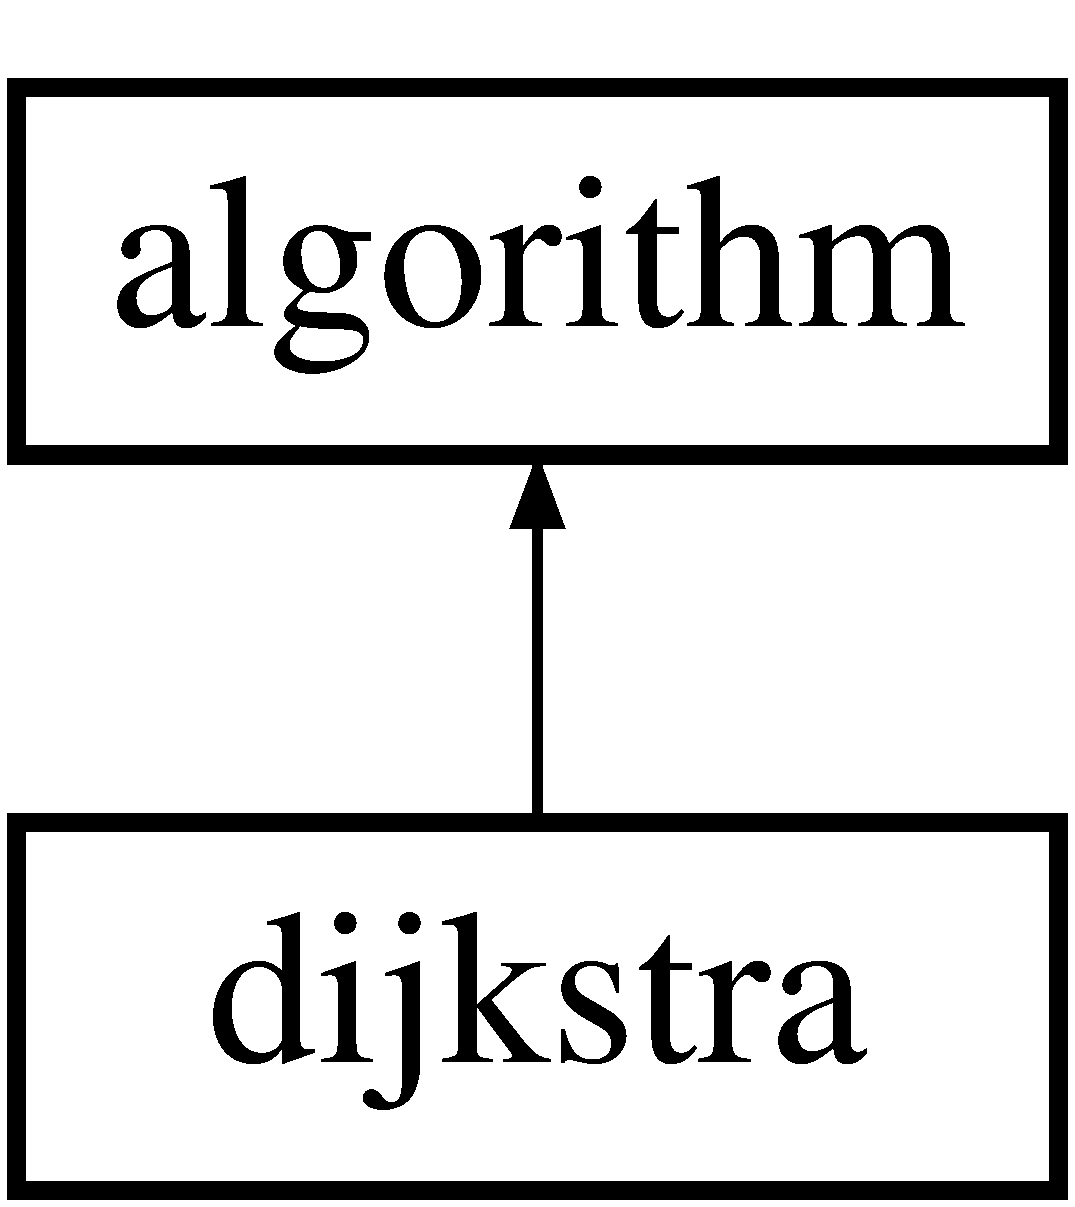
\includegraphics[height=2.000000cm]{classdijkstra}
\end{center}
\end{figure}
\subsection*{Public Types}
\begin{DoxyCompactItemize}
\item 
\mbox{\Hypertarget{classdijkstra_a2bdd8d3b57860b5715d01e65664e810f}\label{classdijkstra_a2bdd8d3b57860b5715d01e65664e810f}} 
enum {\bfseries node\+\_\+color} \{ {\bfseries white}, 
{\bfseries grey}, 
{\bfseries black}
 \}
\item 
\mbox{\Hypertarget{classdijkstra_a5062e9a8339848666efcf2143c4c1881}\label{classdijkstra_a5062e9a8339848666efcf2143c4c1881}} 
typedef list$<$ \mbox{\hyperlink{classnode}{node}} $>$\+::const\+\_\+iterator \mbox{\hyperlink{classdijkstra_a5062e9a8339848666efcf2143c4c1881}{shortest\+\_\+path\+\_\+node\+\_\+iterator}}
\begin{DoxyCompactList}\small\item\em Iterator type for traversing nodes on one shortest path. \end{DoxyCompactList}\item 
\mbox{\Hypertarget{classdijkstra_ad35d95d4ed7a4202a5d048a63aa115b9}\label{classdijkstra_ad35d95d4ed7a4202a5d048a63aa115b9}} 
typedef list$<$ \mbox{\hyperlink{classedge}{edge}} $>$\+::const\+\_\+iterator \mbox{\hyperlink{classdijkstra_ad35d95d4ed7a4202a5d048a63aa115b9}{shortest\+\_\+path\+\_\+edge\+\_\+iterator}}
\begin{DoxyCompactList}\small\item\em Iterator type for traversing edges on one shortest path. \end{DoxyCompactList}\end{DoxyCompactItemize}
\subsection*{Public Member Functions}
\begin{DoxyCompactItemize}
\item 
\mbox{\hyperlink{classdijkstra_a64a1fcb9cca32ff932b9b98a08cff106}{dijkstra}} ()
\begin{DoxyCompactList}\small\item\em Default constructor. \end{DoxyCompactList}\item 
virtual \mbox{\hyperlink{classdijkstra_a871e3c8097b7f0bc17358473b1149515}{$\sim$dijkstra}} ()
\begin{DoxyCompactList}\small\item\em Destructor. \end{DoxyCompactList}\item 
void \mbox{\hyperlink{classdijkstra_a9689f2628f76ddb3747ea18c91bd7041}{source}} (const \mbox{\hyperlink{classnode}{node}} \&n)
\begin{DoxyCompactList}\small\item\em Sets source node. \end{DoxyCompactList}\item 
void \mbox{\hyperlink{classdijkstra_a1e9971d767046306574551a461aa2238}{target}} (const \mbox{\hyperlink{classnode}{node}} \&n)
\begin{DoxyCompactList}\small\item\em Sets target node. \end{DoxyCompactList}\item 
void \mbox{\hyperlink{classdijkstra_a92f4394b757f6ffcb372535114a6cbf6}{weights}} (const \mbox{\hyperlink{classedge__map}{edge\+\_\+map}}$<$ double $>$ \&weight)
\begin{DoxyCompactList}\small\item\em Sets weights of the edges. \end{DoxyCompactList}\item 
void \mbox{\hyperlink{classdijkstra_af79383dbbb6b737afcefd8e32350192d}{store\+\_\+preds}} (bool set)
\begin{DoxyCompactList}\small\item\em Enables or disables the storing of predecessors. \end{DoxyCompactList}\item 
virtual int \mbox{\hyperlink{classdijkstra_a51ff4657e0ddb1ca5231a21e6dea1808}{check}} (\mbox{\hyperlink{classgraph}{graph}} \&G)
\begin{DoxyCompactList}\small\item\em Checks whether the preconditions for Dijkstra are satisfied. \end{DoxyCompactList}\item 
int \mbox{\hyperlink{classdijkstra_a7b30f3d8ad42baae27989bc14befe0d0}{run}} (\mbox{\hyperlink{classgraph}{graph}} \&G)
\begin{DoxyCompactList}\small\item\em Runs shortest path algorithm on {\ttfamily G}. \end{DoxyCompactList}\item 
\mbox{\hyperlink{classnode}{node}} \mbox{\hyperlink{classdijkstra_a69772d19321b5e4deac66174ec546caa}{source}} () const
\begin{DoxyCompactList}\small\item\em Returns source node. \end{DoxyCompactList}\item 
\mbox{\hyperlink{classnode}{node}} \mbox{\hyperlink{classdijkstra_a4957ef4369386ef2153359ea97da9d88}{target}} () const
\begin{DoxyCompactList}\small\item\em Returns target node if set, {\ttfamily \mbox{\hyperlink{classnode_ad603259398d5667e3b97a6322a2bcc20}{node\+::node()}}} else. \end{DoxyCompactList}\item 
bool \mbox{\hyperlink{classdijkstra_a8ef3ee087994a56b774f48fd331725a3}{store\+\_\+preds}} () const
\begin{DoxyCompactList}\small\item\em Returns whether the storing of predecessors is enabled. \end{DoxyCompactList}\item 
bool \mbox{\hyperlink{classdijkstra_a405ff80abfc9ad98668534032eed6a5b}{reached}} (const \mbox{\hyperlink{classnode}{node}} \&n) const
\begin{DoxyCompactList}\small\item\em Returns whether {\ttfamily n} is reachable from source node. \end{DoxyCompactList}\item 
double \mbox{\hyperlink{classdijkstra_ae350a266dd47091d7f620a7328619426}{distance}} (const \mbox{\hyperlink{classnode}{node}} \&n) const
\begin{DoxyCompactList}\small\item\em Returns the distance from source node to node {\ttfamily n}. \end{DoxyCompactList}\item 
\mbox{\hyperlink{classnode}{node}} \mbox{\hyperlink{classdijkstra_a99c17ee7c2b55574ea8c2952fac09faf}{predecessor\+\_\+node}} (const \mbox{\hyperlink{classnode}{node}} \&n) const
\begin{DoxyCompactList}\small\item\em Predecessor node of node {\ttfamily n} on the shortest path from the source node. \end{DoxyCompactList}\item 
\mbox{\hyperlink{classedge}{edge}} \mbox{\hyperlink{classdijkstra_aa3ef1a7d7dfc33e4a39aff309f873929}{predecessor\+\_\+edge}} (const \mbox{\hyperlink{classnode}{node}} \&n) const
\begin{DoxyCompactList}\small\item\em Predecessor edge of node {\ttfamily n} on the shortest path from the source node. \end{DoxyCompactList}\item 
\mbox{\hyperlink{classdijkstra_a5062e9a8339848666efcf2143c4c1881}{shortest\+\_\+path\+\_\+node\+\_\+iterator}} \mbox{\hyperlink{classdijkstra_ae30c66319d925387ed858aab9ce419ae}{shortest\+\_\+path\+\_\+nodes\+\_\+begin}} (const \mbox{\hyperlink{classnode}{node}} \&dest)
\begin{DoxyCompactList}\small\item\em Returns an iterator to the beginning (to the source node) of a shortest node path to node {\ttfamily dest}. \end{DoxyCompactList}\item 
\mbox{\hyperlink{classdijkstra_a5062e9a8339848666efcf2143c4c1881}{shortest\+\_\+path\+\_\+node\+\_\+iterator}} \mbox{\hyperlink{classdijkstra_ae9846beeabd53a8cf0c0c1af328235b2}{shortest\+\_\+path\+\_\+nodes\+\_\+end}} (const \mbox{\hyperlink{classnode}{node}} \&dest)
\begin{DoxyCompactList}\small\item\em Returns an iterator one after the end (one after node {\ttfamily dest}) of a shortest node path to node {\ttfamily dest}. \end{DoxyCompactList}\item 
\mbox{\hyperlink{classdijkstra_ad35d95d4ed7a4202a5d048a63aa115b9}{shortest\+\_\+path\+\_\+edge\+\_\+iterator}} \mbox{\hyperlink{classdijkstra_ad7ef6f747b68f8951322b265844dbb8a}{shortest\+\_\+path\+\_\+edges\+\_\+begin}} (const \mbox{\hyperlink{classnode}{node}} \&dest)
\begin{DoxyCompactList}\small\item\em Returns an iterator to the beginning edge of a shortest edge path to node {\ttfamily dest}. \end{DoxyCompactList}\item 
\mbox{\hyperlink{classdijkstra_ad35d95d4ed7a4202a5d048a63aa115b9}{shortest\+\_\+path\+\_\+edge\+\_\+iterator}} \mbox{\hyperlink{classdijkstra_a031e6fef10aa40aad10edc1053ad9cf0}{shortest\+\_\+path\+\_\+edges\+\_\+end}} (const \mbox{\hyperlink{classnode}{node}} \&dest)
\begin{DoxyCompactList}\small\item\em Returns an iterator one after the end of a shortest edge path to node {\ttfamily dest}. \end{DoxyCompactList}\item 
virtual void \mbox{\hyperlink{classdijkstra_a444c288b3a49ec1c2973459dad55ffb3}{reset}} ()
\begin{DoxyCompactList}\small\item\em Resets Dijkstra\textquotesingle{}s algorithm. \end{DoxyCompactList}\end{DoxyCompactItemize}


\subsection{Detailed Description}
Dijkstra\textquotesingle{}s Algorithm for computing single source shortest path. 

This class implements Dijkstra\textquotesingle{}s algorithm for computing single source shortest path in $\mathcal{O}((|V| + |E|) log |V|)$ worst case.

\begin{DoxySeeAlso}{See also}
\mbox{\hyperlink{classbellman__ford}{bellman\+\_\+ford}}
\end{DoxySeeAlso}
\begin{DoxyAuthor}{Author}
Stf Kolev \href{mailto:inkyzfx@gmail.com}{\tt inkyzfx@gmail.\+com} 
\end{DoxyAuthor}


\subsection{Constructor \& Destructor Documentation}
\mbox{\Hypertarget{classdijkstra_a64a1fcb9cca32ff932b9b98a08cff106}\label{classdijkstra_a64a1fcb9cca32ff932b9b98a08cff106}} 
\index{dijkstra@{dijkstra}!dijkstra@{dijkstra}}
\index{dijkstra@{dijkstra}!dijkstra@{dijkstra}}
\subsubsection{\texorpdfstring{dijkstra()}{dijkstra()}}
{\footnotesize\ttfamily dijkstra\+::dijkstra (\begin{DoxyParamCaption}{ }\end{DoxyParamCaption})}



Default constructor. 

Enables only the calculation of shortest paths.

\begin{DoxySeeAlso}{See also}
\mbox{\hyperlink{classalgorithm_ab79e1ddec2f2afdf4b36b10724db8b15}{algorithm\+::algorithm}} 
\end{DoxySeeAlso}
\mbox{\Hypertarget{classdijkstra_a871e3c8097b7f0bc17358473b1149515}\label{classdijkstra_a871e3c8097b7f0bc17358473b1149515}} 
\index{dijkstra@{dijkstra}!````~dijkstra@{$\sim$dijkstra}}
\index{````~dijkstra@{$\sim$dijkstra}!dijkstra@{dijkstra}}
\subsubsection{\texorpdfstring{$\sim$dijkstra()}{~dijkstra()}}
{\footnotesize\ttfamily dijkstra\+::$\sim$dijkstra (\begin{DoxyParamCaption}{ }\end{DoxyParamCaption})\hspace{0.3cm}{\ttfamily [virtual]}}



Destructor. 

\begin{DoxySeeAlso}{See also}
\mbox{\hyperlink{classalgorithm_adca9b1e7fa3afd914519a9dbb44e9fd5}{algorithm\+::$\sim$algorithm}} 
\end{DoxySeeAlso}


\subsection{Member Function Documentation}
\mbox{\Hypertarget{classdijkstra_a51ff4657e0ddb1ca5231a21e6dea1808}\label{classdijkstra_a51ff4657e0ddb1ca5231a21e6dea1808}} 
\index{dijkstra@{dijkstra}!check@{check}}
\index{check@{check}!dijkstra@{dijkstra}}
\subsubsection{\texorpdfstring{check()}{check()}}
{\footnotesize\ttfamily int dijkstra\+::check (\begin{DoxyParamCaption}\item[{\mbox{\hyperlink{classgraph}{graph}} \&}]{G }\end{DoxyParamCaption})\hspace{0.3cm}{\ttfamily [virtual]}}



Checks whether the preconditions for Dijkstra are satisfied. 

Necessary preconditions are\+:
\begin{DoxyItemize}
\item the weights of the edges are set
\item the graph {\ttfamily G} has at least one node
\item all edge weights must be $\ge 0$
\item the source node and (if set) target node must be found in {\ttfamily G} 
\end{DoxyItemize}


\begin{DoxyParams}{Parameters}
{\em G} & graph\\
\hline
\end{DoxyParams}

\begin{DoxyRetVals}{Return values}
{\em \mbox{\hyperlink{classalgorithm_af1a0078e153aa99c24f9bdf0d97f6710aae4c1cd7fe8d8cf4b143241a6e7c31cf}{algorithm\+::\+K\+G\+L\+\_\+\+OK}}} & if algorithm can be applied \\
\hline
{\em \mbox{\hyperlink{classalgorithm_af1a0078e153aa99c24f9bdf0d97f6710ae67bf27b2ef31f73e545a7f9f4a69556}{algorithm\+::\+K\+G\+L\+\_\+\+E\+R\+R\+OR}}} & otherwise\\
\hline
\end{DoxyRetVals}
\begin{DoxySeeAlso}{See also}
\mbox{\hyperlink{classdijkstra_a9689f2628f76ddb3747ea18c91bd7041}{dijkstra\+::source}} 

\mbox{\hyperlink{classdijkstra_a92f4394b757f6ffcb372535114a6cbf6}{dijkstra\+::weights}} 

\mbox{\hyperlink{classalgorithm_a76361fb03ad1cf643affc51821e43bed}{algorithm\+::check}} 
\end{DoxySeeAlso}


Implements \mbox{\hyperlink{classalgorithm_a76361fb03ad1cf643affc51821e43bed}{algorithm}}.

\mbox{\Hypertarget{classdijkstra_ae350a266dd47091d7f620a7328619426}\label{classdijkstra_ae350a266dd47091d7f620a7328619426}} 
\index{dijkstra@{dijkstra}!distance@{distance}}
\index{distance@{distance}!dijkstra@{dijkstra}}
\subsubsection{\texorpdfstring{distance()}{distance()}}
{\footnotesize\ttfamily double dijkstra\+::distance (\begin{DoxyParamCaption}\item[{const \mbox{\hyperlink{classnode}{node}} \&}]{n }\end{DoxyParamCaption}) const}



Returns the distance from source node to node {\ttfamily n}. 


\begin{DoxyParams}{Parameters}
{\em n} & node\\
\hline
\end{DoxyParams}
\begin{DoxyReturn}{Returns}
distance if {\ttfamily n} is \mbox{\hyperlink{classdijkstra_a405ff80abfc9ad98668534032eed6a5b}{dijkstra\+::reached}}, {\ttfamily -\/1.\+0} else 
\end{DoxyReturn}
\mbox{\Hypertarget{classdijkstra_aa3ef1a7d7dfc33e4a39aff309f873929}\label{classdijkstra_aa3ef1a7d7dfc33e4a39aff309f873929}} 
\index{dijkstra@{dijkstra}!predecessor\+\_\+edge@{predecessor\+\_\+edge}}
\index{predecessor\+\_\+edge@{predecessor\+\_\+edge}!dijkstra@{dijkstra}}
\subsubsection{\texorpdfstring{predecessor\+\_\+edge()}{predecessor\_edge()}}
{\footnotesize\ttfamily \mbox{\hyperlink{classedge}{edge}} dijkstra\+::predecessor\+\_\+edge (\begin{DoxyParamCaption}\item[{const \mbox{\hyperlink{classnode}{node}} \&}]{n }\end{DoxyParamCaption}) const}



Predecessor edge of node {\ttfamily n} on the shortest path from the source node. 

If {\ttfamily n} is a root or wasn\textquotesingle{}t reached the return value is the invalid edge \mbox{\hyperlink{classedge_a41859d2473a15e24255d7bc0de1f49b4}{edge\+::edge()}}.


\begin{DoxyParams}{Parameters}
{\em n} & node\\
\hline
\end{DoxyParams}
\begin{DoxyReturn}{Returns}
predecessor edge of {\ttfamily n} 
\end{DoxyReturn}
\begin{DoxySeeAlso}{See also}
\mbox{\hyperlink{classdijkstra_af79383dbbb6b737afcefd8e32350192d}{dijkstra\+::store\+\_\+preds}} 

\mbox{\hyperlink{classdijkstra_a99c17ee7c2b55574ea8c2952fac09faf}{dijkstra\+::predecessor\+\_\+node}}
\end{DoxySeeAlso}
\begin{DoxyNote}{Note}
The method requires that predecessor calculation option was enabled during last run. 
\end{DoxyNote}
\mbox{\Hypertarget{classdijkstra_a99c17ee7c2b55574ea8c2952fac09faf}\label{classdijkstra_a99c17ee7c2b55574ea8c2952fac09faf}} 
\index{dijkstra@{dijkstra}!predecessor\+\_\+node@{predecessor\+\_\+node}}
\index{predecessor\+\_\+node@{predecessor\+\_\+node}!dijkstra@{dijkstra}}
\subsubsection{\texorpdfstring{predecessor\+\_\+node()}{predecessor\_node()}}
{\footnotesize\ttfamily \mbox{\hyperlink{classnode}{node}} dijkstra\+::predecessor\+\_\+node (\begin{DoxyParamCaption}\item[{const \mbox{\hyperlink{classnode}{node}} \&}]{n }\end{DoxyParamCaption}) const}



Predecessor node of node {\ttfamily n} on the shortest path from the source node. 

If {\ttfamily n} is a root or wasn\textquotesingle{}t reached the return value is the invalid node \mbox{\hyperlink{classnode_ad603259398d5667e3b97a6322a2bcc20}{node\+::node()}}.


\begin{DoxyParams}{Parameters}
{\em n} & node\\
\hline
\end{DoxyParams}
\begin{DoxyReturn}{Returns}
predecessor node of {\ttfamily n} 
\end{DoxyReturn}
\begin{DoxySeeAlso}{See also}
\mbox{\hyperlink{classdijkstra_af79383dbbb6b737afcefd8e32350192d}{dijkstra\+::store\+\_\+preds}} 

\mbox{\hyperlink{classdijkstra_aa3ef1a7d7dfc33e4a39aff309f873929}{dijkstra\+::predecessor\+\_\+edge}}
\end{DoxySeeAlso}
\begin{DoxyNote}{Note}
The method requires that predecessor calculation option was enabled during last run. 
\end{DoxyNote}
\mbox{\Hypertarget{classdijkstra_a405ff80abfc9ad98668534032eed6a5b}\label{classdijkstra_a405ff80abfc9ad98668534032eed6a5b}} 
\index{dijkstra@{dijkstra}!reached@{reached}}
\index{reached@{reached}!dijkstra@{dijkstra}}
\subsubsection{\texorpdfstring{reached()}{reached()}}
{\footnotesize\ttfamily bool dijkstra\+::reached (\begin{DoxyParamCaption}\item[{const \mbox{\hyperlink{classnode}{node}} \&}]{n }\end{DoxyParamCaption}) const}



Returns whether {\ttfamily n} is reachable from source node. 


\begin{DoxyParams}{Parameters}
{\em n} & node\\
\hline
\end{DoxyParams}
\begin{DoxyReturn}{Returns}
{\ttfamily true} iff {\ttfamily n} was reached from source 
\end{DoxyReturn}
\mbox{\Hypertarget{classdijkstra_a444c288b3a49ec1c2973459dad55ffb3}\label{classdijkstra_a444c288b3a49ec1c2973459dad55ffb3}} 
\index{dijkstra@{dijkstra}!reset@{reset}}
\index{reset@{reset}!dijkstra@{dijkstra}}
\subsubsection{\texorpdfstring{reset()}{reset()}}
{\footnotesize\ttfamily void dijkstra\+::reset (\begin{DoxyParamCaption}{ }\end{DoxyParamCaption})\hspace{0.3cm}{\ttfamily [virtual]}}



Resets Dijkstra\textquotesingle{}s algorithm. 

It prepares the algorithm to be applied again, possibly to another graph.

\begin{DoxyNote}{Note}
The weights are not reset. You can apply this algorithms
\end{DoxyNote}
\begin{DoxySeeAlso}{See also}
\mbox{\hyperlink{classalgorithm_a21aba63d066ae7897de6ca7d8425c408}{algorithm\+::reset}} 
\end{DoxySeeAlso}


Implements \mbox{\hyperlink{classalgorithm_a21aba63d066ae7897de6ca7d8425c408}{algorithm}}.

\mbox{\Hypertarget{classdijkstra_a7b30f3d8ad42baae27989bc14befe0d0}\label{classdijkstra_a7b30f3d8ad42baae27989bc14befe0d0}} 
\index{dijkstra@{dijkstra}!run@{run}}
\index{run@{run}!dijkstra@{dijkstra}}
\subsubsection{\texorpdfstring{run()}{run()}}
{\footnotesize\ttfamily int dijkstra\+::run (\begin{DoxyParamCaption}\item[{\mbox{\hyperlink{classgraph}{graph}} \&}]{G }\end{DoxyParamCaption})\hspace{0.3cm}{\ttfamily [virtual]}}



Runs shortest path algorithm on {\ttfamily G}. 

This should return always \mbox{\hyperlink{classalgorithm_af1a0078e153aa99c24f9bdf0d97f6710aae4c1cd7fe8d8cf4b143241a6e7c31cf}{algorithm\+::\+K\+G\+L\+\_\+\+OK}}. The return value only tracks errors that might occur. Afterwards the result of the test can be accessed via access methods.


\begin{DoxyParams}{Parameters}
{\em G} & graph\\
\hline
\end{DoxyParams}

\begin{DoxyRetVals}{Return values}
{\em \mbox{\hyperlink{classalgorithm_af1a0078e153aa99c24f9bdf0d97f6710aae4c1cd7fe8d8cf4b143241a6e7c31cf}{algorithm\+::\+K\+G\+L\+\_\+\+OK}}} & on success \\
\hline
{\em \mbox{\hyperlink{classalgorithm_af1a0078e153aa99c24f9bdf0d97f6710ae67bf27b2ef31f73e545a7f9f4a69556}{algorithm\+::\+K\+G\+L\+\_\+\+E\+R\+R\+OR}}} & otherwise\\
\hline
\end{DoxyRetVals}
\begin{DoxySeeAlso}{See also}
\mbox{\hyperlink{classalgorithm_a734b189509a8d6b56b65f8ff772d43ca}{algorithm\+::run}} 
\end{DoxySeeAlso}


Implements \mbox{\hyperlink{classalgorithm_a734b189509a8d6b56b65f8ff772d43ca}{algorithm}}.

\mbox{\Hypertarget{classdijkstra_ad7ef6f747b68f8951322b265844dbb8a}\label{classdijkstra_ad7ef6f747b68f8951322b265844dbb8a}} 
\index{dijkstra@{dijkstra}!shortest\+\_\+path\+\_\+edges\+\_\+begin@{shortest\+\_\+path\+\_\+edges\+\_\+begin}}
\index{shortest\+\_\+path\+\_\+edges\+\_\+begin@{shortest\+\_\+path\+\_\+edges\+\_\+begin}!dijkstra@{dijkstra}}
\subsubsection{\texorpdfstring{shortest\+\_\+path\+\_\+edges\+\_\+begin()}{shortest\_path\_edges\_begin()}}
{\footnotesize\ttfamily \mbox{\hyperlink{classdijkstra_ad35d95d4ed7a4202a5d048a63aa115b9}{dijkstra\+::shortest\+\_\+path\+\_\+edge\+\_\+iterator}} dijkstra\+::shortest\+\_\+path\+\_\+edges\+\_\+begin (\begin{DoxyParamCaption}\item[{const \mbox{\hyperlink{classnode}{node}} \&}]{dest }\end{DoxyParamCaption})}



Returns an iterator to the beginning edge of a shortest edge path to node {\ttfamily dest}. 


\begin{DoxyParams}{Parameters}
{\em dest} & target node\\
\hline
\end{DoxyParams}
\begin{DoxyReturn}{Returns}
beginning edge iterator of a shortest path
\end{DoxyReturn}
\begin{DoxyNote}{Note}
The method requires that predecessor calculation option was enabled during last run. If this method is called on the shortest path to {\ttfamily dest} for the first time (before \mbox{\hyperlink{classdijkstra_a031e6fef10aa40aad10edc1053ad9cf0}{dijkstra\+::shortest\+\_\+path\+\_\+edges\+\_\+end}}) it needs $\mathcal{O}(\mbox{length of this path})$ time. 
\end{DoxyNote}
\mbox{\Hypertarget{classdijkstra_a031e6fef10aa40aad10edc1053ad9cf0}\label{classdijkstra_a031e6fef10aa40aad10edc1053ad9cf0}} 
\index{dijkstra@{dijkstra}!shortest\+\_\+path\+\_\+edges\+\_\+end@{shortest\+\_\+path\+\_\+edges\+\_\+end}}
\index{shortest\+\_\+path\+\_\+edges\+\_\+end@{shortest\+\_\+path\+\_\+edges\+\_\+end}!dijkstra@{dijkstra}}
\subsubsection{\texorpdfstring{shortest\+\_\+path\+\_\+edges\+\_\+end()}{shortest\_path\_edges\_end()}}
{\footnotesize\ttfamily \mbox{\hyperlink{classdijkstra_ad35d95d4ed7a4202a5d048a63aa115b9}{dijkstra\+::shortest\+\_\+path\+\_\+edge\+\_\+iterator}} dijkstra\+::shortest\+\_\+path\+\_\+edges\+\_\+end (\begin{DoxyParamCaption}\item[{const \mbox{\hyperlink{classnode}{node}} \&}]{dest }\end{DoxyParamCaption})}



Returns an iterator one after the end of a shortest edge path to node {\ttfamily dest}. 


\begin{DoxyParams}{Parameters}
{\em dest} & target node\\
\hline
\end{DoxyParams}
\begin{DoxyReturn}{Returns}
shortest path end edge iterator
\end{DoxyReturn}
\begin{DoxyNote}{Note}
The method requires that predecessor calculation option was enabled during last run. If this method is called on the shortest path to {\ttfamily dest} for the first time (before \mbox{\hyperlink{classdijkstra_ad7ef6f747b68f8951322b265844dbb8a}{dijkstra\+::shortest\+\_\+path\+\_\+edges\+\_\+begin}}) it needs $\mathcal{O}(\mbox{length of this path})$ time. 
\end{DoxyNote}
\mbox{\Hypertarget{classdijkstra_ae30c66319d925387ed858aab9ce419ae}\label{classdijkstra_ae30c66319d925387ed858aab9ce419ae}} 
\index{dijkstra@{dijkstra}!shortest\+\_\+path\+\_\+nodes\+\_\+begin@{shortest\+\_\+path\+\_\+nodes\+\_\+begin}}
\index{shortest\+\_\+path\+\_\+nodes\+\_\+begin@{shortest\+\_\+path\+\_\+nodes\+\_\+begin}!dijkstra@{dijkstra}}
\subsubsection{\texorpdfstring{shortest\+\_\+path\+\_\+nodes\+\_\+begin()}{shortest\_path\_nodes\_begin()}}
{\footnotesize\ttfamily \mbox{\hyperlink{classdijkstra_a5062e9a8339848666efcf2143c4c1881}{dijkstra\+::shortest\+\_\+path\+\_\+node\+\_\+iterator}} dijkstra\+::shortest\+\_\+path\+\_\+nodes\+\_\+begin (\begin{DoxyParamCaption}\item[{const \mbox{\hyperlink{classnode}{node}} \&}]{dest }\end{DoxyParamCaption})}



Returns an iterator to the beginning (to the source node) of a shortest node path to node {\ttfamily dest}. 


\begin{DoxyParams}{Parameters}
{\em dest} & target node\\
\hline
\end{DoxyParams}
\begin{DoxyReturn}{Returns}
beginning node iterator of a shortest path
\end{DoxyReturn}
\begin{DoxyNote}{Note}
The method requires that predecessor calculation option was enabled during last run. If this method is called on the shortest path to {\ttfamily dest} for the first time (before \mbox{\hyperlink{classdijkstra_ae9846beeabd53a8cf0c0c1af328235b2}{dijkstra\+::shortest\+\_\+path\+\_\+nodes\+\_\+end}}) it needs $\mathcal{O}(\mbox{length of this path})$ time. 
\end{DoxyNote}
\mbox{\Hypertarget{classdijkstra_ae9846beeabd53a8cf0c0c1af328235b2}\label{classdijkstra_ae9846beeabd53a8cf0c0c1af328235b2}} 
\index{dijkstra@{dijkstra}!shortest\+\_\+path\+\_\+nodes\+\_\+end@{shortest\+\_\+path\+\_\+nodes\+\_\+end}}
\index{shortest\+\_\+path\+\_\+nodes\+\_\+end@{shortest\+\_\+path\+\_\+nodes\+\_\+end}!dijkstra@{dijkstra}}
\subsubsection{\texorpdfstring{shortest\+\_\+path\+\_\+nodes\+\_\+end()}{shortest\_path\_nodes\_end()}}
{\footnotesize\ttfamily \mbox{\hyperlink{classdijkstra_a5062e9a8339848666efcf2143c4c1881}{dijkstra\+::shortest\+\_\+path\+\_\+node\+\_\+iterator}} dijkstra\+::shortest\+\_\+path\+\_\+nodes\+\_\+end (\begin{DoxyParamCaption}\item[{const \mbox{\hyperlink{classnode}{node}} \&}]{dest }\end{DoxyParamCaption})}



Returns an iterator one after the end (one after node {\ttfamily dest}) of a shortest node path to node {\ttfamily dest}. 


\begin{DoxyParams}{Parameters}
{\em dest} & target node\\
\hline
\end{DoxyParams}
\begin{DoxyReturn}{Returns}
shortest path end node iterator
\end{DoxyReturn}
\begin{DoxyNote}{Note}
The method requires that predecessor calculation option was enabled during last run. If this method is called on the shortest path to {\ttfamily dest} for the first time (before \mbox{\hyperlink{classdijkstra_ae30c66319d925387ed858aab9ce419ae}{dijkstra\+::shortest\+\_\+path\+\_\+nodes\+\_\+begin}}) it needs $\mathcal{O}(\mbox{length of this path})$ time. 
\end{DoxyNote}
\mbox{\Hypertarget{classdijkstra_a9689f2628f76ddb3747ea18c91bd7041}\label{classdijkstra_a9689f2628f76ddb3747ea18c91bd7041}} 
\index{dijkstra@{dijkstra}!source@{source}}
\index{source@{source}!dijkstra@{dijkstra}}
\subsubsection{\texorpdfstring{source()}{source()}\hspace{0.1cm}{\footnotesize\ttfamily [1/2]}}
{\footnotesize\ttfamily void dijkstra\+::source (\begin{DoxyParamCaption}\item[{const \mbox{\hyperlink{classnode}{node}} \&}]{n }\end{DoxyParamCaption})}



Sets source node. 

The default source is the invalid node (\mbox{\hyperlink{classnode_ad603259398d5667e3b97a6322a2bcc20}{node\+::node()}}), in this case an arbitrary node is chosen and stored when this algorithm is run.


\begin{DoxyParams}{Parameters}
{\em n} & source node \\
\hline
\end{DoxyParams}
\mbox{\Hypertarget{classdijkstra_a69772d19321b5e4deac66174ec546caa}\label{classdijkstra_a69772d19321b5e4deac66174ec546caa}} 
\index{dijkstra@{dijkstra}!source@{source}}
\index{source@{source}!dijkstra@{dijkstra}}
\subsubsection{\texorpdfstring{source()}{source()}\hspace{0.1cm}{\footnotesize\ttfamily [2/2]}}
{\footnotesize\ttfamily \mbox{\hyperlink{classnode}{node}} dijkstra\+::source (\begin{DoxyParamCaption}{ }\end{DoxyParamCaption}) const}



Returns source node. 

\begin{DoxyReturn}{Returns}
source node 
\end{DoxyReturn}
\mbox{\Hypertarget{classdijkstra_af79383dbbb6b737afcefd8e32350192d}\label{classdijkstra_af79383dbbb6b737afcefd8e32350192d}} 
\index{dijkstra@{dijkstra}!store\+\_\+preds@{store\+\_\+preds}}
\index{store\+\_\+preds@{store\+\_\+preds}!dijkstra@{dijkstra}}
\subsubsection{\texorpdfstring{store\+\_\+preds()}{store\_preds()}\hspace{0.1cm}{\footnotesize\ttfamily [1/2]}}
{\footnotesize\ttfamily void dijkstra\+::store\+\_\+preds (\begin{DoxyParamCaption}\item[{bool}]{set }\end{DoxyParamCaption})}



Enables or disables the storing of predecessors. 

If enabled for every node the predecessor on the shortest path from will be stored.


\begin{DoxyParams}{Parameters}
{\em set} & {\ttfamily true} if predecessors should be stored\\
\hline
\end{DoxyParams}
\begin{DoxySeeAlso}{See also}
\mbox{\hyperlink{classdijkstra_a99c17ee7c2b55574ea8c2952fac09faf}{dijkstra\+::predecessor\+\_\+node}} 

\mbox{\hyperlink{classdijkstra_aa3ef1a7d7dfc33e4a39aff309f873929}{dijkstra\+::predecessor\+\_\+edge}} 
\end{DoxySeeAlso}
\mbox{\Hypertarget{classdijkstra_a8ef3ee087994a56b774f48fd331725a3}\label{classdijkstra_a8ef3ee087994a56b774f48fd331725a3}} 
\index{dijkstra@{dijkstra}!store\+\_\+preds@{store\+\_\+preds}}
\index{store\+\_\+preds@{store\+\_\+preds}!dijkstra@{dijkstra}}
\subsubsection{\texorpdfstring{store\+\_\+preds()}{store\_preds()}\hspace{0.1cm}{\footnotesize\ttfamily [2/2]}}
{\footnotesize\ttfamily bool dijkstra\+::store\+\_\+preds (\begin{DoxyParamCaption}{ }\end{DoxyParamCaption}) const}



Returns whether the storing of predecessors is enabled. 

\begin{DoxyReturn}{Returns}
{\ttfamily true} iff the storing of predecessors is enabled
\end{DoxyReturn}
\begin{DoxySeeAlso}{See also}
dijkstra\+::predecessor 
\end{DoxySeeAlso}
\mbox{\Hypertarget{classdijkstra_a1e9971d767046306574551a461aa2238}\label{classdijkstra_a1e9971d767046306574551a461aa2238}} 
\index{dijkstra@{dijkstra}!target@{target}}
\index{target@{target}!dijkstra@{dijkstra}}
\subsubsection{\texorpdfstring{target()}{target()}\hspace{0.1cm}{\footnotesize\ttfamily [1/2]}}
{\footnotesize\ttfamily void dijkstra\+::target (\begin{DoxyParamCaption}\item[{const \mbox{\hyperlink{classnode}{node}} \&}]{n }\end{DoxyParamCaption})}



Sets target node. 

If a target is set with this method the algorithm stops if a shortest distance to {\ttfamily n} is found. Ohterwise shortest paths are computed from source to any node in the graph.


\begin{DoxyParams}{Parameters}
{\em n} & target node \\
\hline
\end{DoxyParams}
\mbox{\Hypertarget{classdijkstra_a4957ef4369386ef2153359ea97da9d88}\label{classdijkstra_a4957ef4369386ef2153359ea97da9d88}} 
\index{dijkstra@{dijkstra}!target@{target}}
\index{target@{target}!dijkstra@{dijkstra}}
\subsubsection{\texorpdfstring{target()}{target()}\hspace{0.1cm}{\footnotesize\ttfamily [2/2]}}
{\footnotesize\ttfamily \mbox{\hyperlink{classnode}{node}} dijkstra\+::target (\begin{DoxyParamCaption}{ }\end{DoxyParamCaption}) const}



Returns target node if set, {\ttfamily \mbox{\hyperlink{classnode_ad603259398d5667e3b97a6322a2bcc20}{node\+::node()}}} else. 

\begin{DoxyReturn}{Returns}
target node 
\end{DoxyReturn}
\mbox{\Hypertarget{classdijkstra_a92f4394b757f6ffcb372535114a6cbf6}\label{classdijkstra_a92f4394b757f6ffcb372535114a6cbf6}} 
\index{dijkstra@{dijkstra}!weights@{weights}}
\index{weights@{weights}!dijkstra@{dijkstra}}
\subsubsection{\texorpdfstring{weights()}{weights()}}
{\footnotesize\ttfamily void dijkstra\+::weights (\begin{DoxyParamCaption}\item[{const \mbox{\hyperlink{classedge__map}{edge\+\_\+map}}$<$ double $>$ \&}]{weight }\end{DoxyParamCaption})}



Sets weights of the edges. 

This method {\bfseries must} be called before check run.


\begin{DoxyParams}{Parameters}
{\em weight} & weights of the edges \\
\hline
\end{DoxyParams}


The documentation for this class was generated from the following files\+:\begin{DoxyCompactItemize}
\item 
include/\+K\+G\+L/dijkstra.\+h\item 
src/dijkstra.\+cpp\end{DoxyCompactItemize}

\hypertarget{classdirection__indicator}{}\section{direction\+\_\+indicator Class Reference}
\label{classdirection__indicator}\index{direction\+\_\+indicator@{direction\+\_\+indicator}}
Inheritance diagram for direction\+\_\+indicator\+:\begin{figure}[H]
\begin{center}
\leavevmode
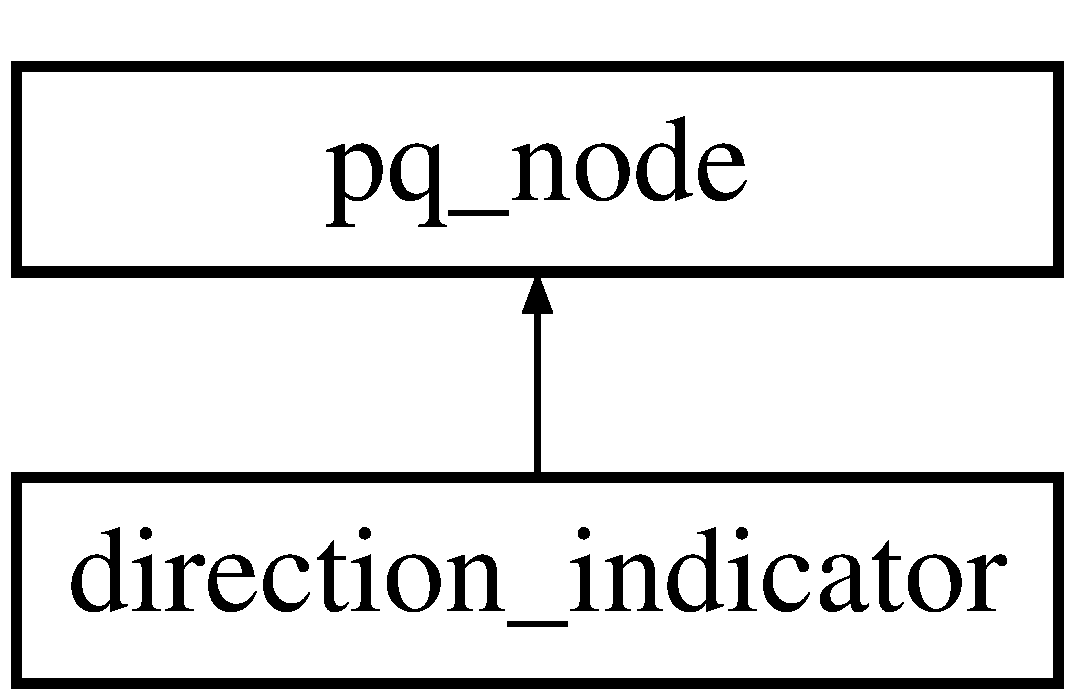
\includegraphics[height=2.000000cm]{classdirection__indicator}
\end{center}
\end{figure}
\subsection*{Friends}
\begin{DoxyCompactItemize}
\item 
\mbox{\Hypertarget{classdirection__indicator_ab6a02224dbc06343d95919289aec77c8}\label{classdirection__indicator_ab6a02224dbc06343d95919289aec77c8}} 
class {\bfseries planarity}
\item 
\mbox{\Hypertarget{classdirection__indicator_a0a5be4bb438c891059fae98f607f2a9c}\label{classdirection__indicator_a0a5be4bb438c891059fae98f607f2a9c}} 
class {\bfseries pq\+\_\+tree}
\end{DoxyCompactItemize}
\subsection*{Additional Inherited Members}


The documentation for this class was generated from the following files\+:\begin{DoxyCompactItemize}
\item 
include/\+K\+G\+L/pq\+\_\+node.\+h\item 
src/pq\+\_\+node.\+cpp\end{DoxyCompactItemize}

\hypertarget{classedge}{}\section{edge Class Reference}
\label{classedge}\index{edge@{edge}}


An edge in a graph.  




{\ttfamily \#include $<$edge.\+h$>$}

\subsection*{Public Member Functions}
\begin{DoxyCompactItemize}
\item 
\mbox{\hyperlink{classedge_a41859d2473a15e24255d7bc0de1f49b4}{edge}} ()
\item 
\mbox{\hyperlink{classnode}{node}} \mbox{\hyperlink{classedge_ae82d5701f7e6f71edc3c8b0e34bcd2b7}{source}} () const
\item 
\mbox{\hyperlink{classnode}{node}} \mbox{\hyperlink{classedge_a97563b611261478ee19c6ce055f1a3ee}{target}} () const
\item 
void \mbox{\hyperlink{classedge_ad62516eb40dbee9f57a2078cfd97b4c9}{reverse}} ()
\item 
void \mbox{\hyperlink{classedge_ad9e615b1a11bbc88aae2b166d377f354}{change\+\_\+source}} (\mbox{\hyperlink{classnode}{node}} n)
\item 
void \mbox{\hyperlink{classedge_a2f797fda0f41412265d793982f2cf953}{change\+\_\+target}} (\mbox{\hyperlink{classnode}{node}} n)
\item 
const \mbox{\hyperlink{classnode}{node}} \& \mbox{\hyperlink{classedge_ab64dc3659c9003337b0c3749a8b879cf}{opposite}} (\mbox{\hyperlink{classnode}{node}} n) const
\item 
\mbox{\Hypertarget{classedge_a01481a54b506f99dfad3ab64bc16715d}\label{classedge_a01481a54b506f99dfad3ab64bc16715d}} 
list$<$ \mbox{\hyperlink{classnode}{node}} $>$ {\bfseries sources} () const
\item 
\mbox{\Hypertarget{classedge_a2f0aa8c08e508f81734e360710237639}\label{classedge_a2f0aa8c08e508f81734e360710237639}} 
list$<$ \mbox{\hyperlink{classnode}{node}} $>$ {\bfseries targets} () const
\item 
\mbox{\Hypertarget{classedge_aa7635988ab396748d6081ae5d273923b}\label{classedge_aa7635988ab396748d6081ae5d273923b}} 
int {\bfseries id} () const
\item 
bool \mbox{\hyperlink{classedge_ab6d6192a90b1cb77ce9dee2de78d9743}{is\+\_\+hidden}} () const
\end{DoxyCompactItemize}
\subsection*{Friends}
\begin{DoxyCompactItemize}
\item 
\mbox{\Hypertarget{classedge_ab8b0dbc1b36724e5e4635ac651c218cb}\label{classedge_ab8b0dbc1b36724e5e4635ac651c218cb}} 
class {\bfseries graph}
\item 
\mbox{\Hypertarget{classedge_a3700a7180235e9a28534b15d5922de12}\label{classedge_a3700a7180235e9a28534b15d5922de12}} 
class {\bfseries node}
\item 
\mbox{\Hypertarget{classedge_a5f37f74566982c3d5a9cef99e3aaee96}\label{classedge_a5f37f74566982c3d5a9cef99e3aaee96}} 
K\+G\+L\+\_\+\+E\+X\+T\+E\+RN friend bool {\bfseries operator==} (\mbox{\hyperlink{classedge}{edge}}, \mbox{\hyperlink{classedge}{edge}})
\item 
\mbox{\Hypertarget{classedge_aadb4c4480975d97b365253a6e835b4cd}\label{classedge_aadb4c4480975d97b365253a6e835b4cd}} 
K\+G\+L\+\_\+\+E\+X\+T\+E\+RN friend bool {\bfseries operator!=} (\mbox{\hyperlink{classedge}{edge}}, \mbox{\hyperlink{classedge}{edge}})
\item 
\mbox{\Hypertarget{classedge_af5dab224b905b68f4314b9e3749ed33a}\label{classedge_af5dab224b905b68f4314b9e3749ed33a}} 
K\+G\+L\+\_\+\+E\+X\+T\+E\+RN friend bool {\bfseries operator$<$} (\mbox{\hyperlink{classedge}{edge}}, \mbox{\hyperlink{classedge}{edge}})
\item 
\mbox{\Hypertarget{classedge_a624b886c3a590296dce64bd09865193e}\label{classedge_a624b886c3a590296dce64bd09865193e}} 
K\+G\+L\+\_\+\+E\+X\+T\+E\+RN friend ostream \& {\bfseries operator$<$$<$} (ostream \&os, const \mbox{\hyperlink{classedge}{edge}} \&e)
\end{DoxyCompactItemize}


\subsection{Detailed Description}
An edge in a graph. 

\subsection{Constructor \& Destructor Documentation}
\mbox{\Hypertarget{classedge_a41859d2473a15e24255d7bc0de1f49b4}\label{classedge_a41859d2473a15e24255d7bc0de1f49b4}} 
\index{edge@{edge}!edge@{edge}}
\index{edge@{edge}!edge@{edge}}
\subsubsection{\texorpdfstring{edge()}{edge()}}
{\footnotesize\ttfamily \+\_\+\+\_\+\+K\+G\+L\+\_\+\+B\+E\+G\+I\+N\+\_\+\+N\+A\+M\+E\+S\+P\+A\+CE edge\+::edge (\begin{DoxyParamCaption}{ }\end{DoxyParamCaption})}

Default constructor. Creates an invalid edge. The only way to obtain a valid edge is through \mbox{\hyperlink{classgraph_a02a0c3a219f75d68caa408ef339d4a1c}{graph\+::new\+\_\+edge}}. Example\+: 
\begin{DoxyPre}
  graph g;
  node n1, n2;
  edge e;\end{DoxyPre}



\begin{DoxyPre}  n1 = g.new\_node();
  n2 = g.new\_node();
  e = g.new\_edge(n1, n2);
\end{DoxyPre}


\begin{DoxySeeAlso}{See also}
\mbox{\hyperlink{classgraph_a02a0c3a219f75d68caa408ef339d4a1c}{graph\+::new\+\_\+edge}} 
\end{DoxySeeAlso}


\subsection{Member Function Documentation}
\mbox{\Hypertarget{classedge_ad9e615b1a11bbc88aae2b166d377f354}\label{classedge_ad9e615b1a11bbc88aae2b166d377f354}} 
\index{edge@{edge}!change\+\_\+source@{change\+\_\+source}}
\index{change\+\_\+source@{change\+\_\+source}!edge@{edge}}
\subsubsection{\texorpdfstring{change\+\_\+source()}{change\_source()}}
{\footnotesize\ttfamily void edge\+::change\+\_\+source (\begin{DoxyParamCaption}\item[{\mbox{\hyperlink{classnode}{node}}}]{n }\end{DoxyParamCaption})}

Makes {\ttfamily n} the source of this edge. Takes O(1) time.


\begin{DoxyParams}{Parameters}
{\em $<$code$>$n$<$/code$>$} & new source \\
\hline
\end{DoxyParams}
\mbox{\Hypertarget{classedge_a2f797fda0f41412265d793982f2cf953}\label{classedge_a2f797fda0f41412265d793982f2cf953}} 
\index{edge@{edge}!change\+\_\+target@{change\+\_\+target}}
\index{change\+\_\+target@{change\+\_\+target}!edge@{edge}}
\subsubsection{\texorpdfstring{change\+\_\+target()}{change\_target()}}
{\footnotesize\ttfamily void edge\+::change\+\_\+target (\begin{DoxyParamCaption}\item[{\mbox{\hyperlink{classnode}{node}}}]{n }\end{DoxyParamCaption})}

Makes {\ttfamily n} the target of this edge. Takes O(1) time.


\begin{DoxyParams}{Parameters}
{\em $<$code$>$n$<$/code$>$} & new target \\
\hline
\end{DoxyParams}
\mbox{\Hypertarget{classedge_ab6d6192a90b1cb77ce9dee2de78d9743}\label{classedge_ab6d6192a90b1cb77ce9dee2de78d9743}} 
\index{edge@{edge}!is\+\_\+hidden@{is\+\_\+hidden}}
\index{is\+\_\+hidden@{is\+\_\+hidden}!edge@{edge}}
\subsubsection{\texorpdfstring{is\+\_\+hidden()}{is\_hidden()}}
{\footnotesize\ttfamily bool edge\+::is\+\_\+hidden (\begin{DoxyParamCaption}{ }\end{DoxyParamCaption}) const}

Returns true iff node is hidden.

\begin{DoxyReturn}{Returns}
true iff node is hidden. 
\end{DoxyReturn}
\begin{DoxySeeAlso}{See also}
\mbox{\hyperlink{classgraph_ab2f8520bcac080d73c55228fecc61825}{graph\+::hide\+\_\+edge}} 

\mbox{\hyperlink{classgraph_a2e5426682a0897b9f9104b019970bedc}{graph\+::restore\+\_\+edge}} 
\end{DoxySeeAlso}
\mbox{\Hypertarget{classedge_ab64dc3659c9003337b0c3749a8b879cf}\label{classedge_ab64dc3659c9003337b0c3749a8b879cf}} 
\index{edge@{edge}!opposite@{opposite}}
\index{opposite@{opposite}!edge@{edge}}
\subsubsection{\texorpdfstring{opposite()}{opposite()}}
{\footnotesize\ttfamily const \mbox{\hyperlink{classnode}{node}} \& edge\+::opposite (\begin{DoxyParamCaption}\item[{\mbox{\hyperlink{classnode}{node}}}]{n }\end{DoxyParamCaption}) const}

Returns the node opposite to {\ttfamily n} referring to this edge.


\begin{DoxyParams}{Parameters}
{\em $<$code$>$n$<$/code$>$} & a node incident to this edge \\
\hline
\end{DoxyParams}
\mbox{\Hypertarget{classedge_ad62516eb40dbee9f57a2078cfd97b4c9}\label{classedge_ad62516eb40dbee9f57a2078cfd97b4c9}} 
\index{edge@{edge}!reverse@{reverse}}
\index{reverse@{reverse}!edge@{edge}}
\subsubsection{\texorpdfstring{reverse()}{reverse()}}
{\footnotesize\ttfamily void edge\+::reverse (\begin{DoxyParamCaption}{ }\end{DoxyParamCaption})}

Changes the direction of this edge. \mbox{\Hypertarget{classedge_ae82d5701f7e6f71edc3c8b0e34bcd2b7}\label{classedge_ae82d5701f7e6f71edc3c8b0e34bcd2b7}} 
\index{edge@{edge}!source@{source}}
\index{source@{source}!edge@{edge}}
\subsubsection{\texorpdfstring{source()}{source()}}
{\footnotesize\ttfamily \mbox{\hyperlink{classnode}{node}} edge\+::source (\begin{DoxyParamCaption}{ }\end{DoxyParamCaption}) const}

Returns the source node of the edge.

\begin{DoxyReturn}{Returns}
source 
\end{DoxyReturn}
\mbox{\Hypertarget{classedge_a97563b611261478ee19c6ce055f1a3ee}\label{classedge_a97563b611261478ee19c6ce055f1a3ee}} 
\index{edge@{edge}!target@{target}}
\index{target@{target}!edge@{edge}}
\subsubsection{\texorpdfstring{target()}{target()}}
{\footnotesize\ttfamily \mbox{\hyperlink{classnode}{node}} edge\+::target (\begin{DoxyParamCaption}{ }\end{DoxyParamCaption}) const}

Returns the target node of the edge.

\begin{DoxyReturn}{Returns}
target 
\end{DoxyReturn}


The documentation for this class was generated from the following files\+:\begin{DoxyCompactItemize}
\item 
include/\+K\+G\+L/edge.\+h\item 
src/edge.\+cpp\end{DoxyCompactItemize}

\hypertarget{classedge__data}{}\section{edge\+\_\+data Class Reference}
\label{classedge__data}\index{edge\+\_\+data@{edge\+\_\+data}}
\subsection*{Public Attributes}
\begin{DoxyCompactItemize}
\item 
\mbox{\Hypertarget{classedge__data_a33597ce417f8d86697b03fc8b6fea526}\label{classedge__data_a33597ce417f8d86697b03fc8b6fea526}} 
int {\bfseries id}
\item 
\mbox{\Hypertarget{classedge__data_a57692abe3b0672d8020e7554a76a0f35}\label{classedge__data_a57692abe3b0672d8020e7554a76a0f35}} 
list$<$ \mbox{\hyperlink{classnode}{node}} $>$ {\bfseries nodes} \mbox{[}2\mbox{]}
\item 
\mbox{\Hypertarget{classedge__data_a49960df0462c61f8830e76c65eb85cce}\label{classedge__data_a49960df0462c61f8830e76c65eb85cce}} 
list$<$ list$<$ \mbox{\hyperlink{classedge}{edge}} $>$\+::iterator $>$ {\bfseries adj\+\_\+pos} \mbox{[}2\mbox{]}
\item 
\mbox{\Hypertarget{classedge__data_acc25b12e22f5568a90b216d4deca90b5}\label{classedge__data_acc25b12e22f5568a90b216d4deca90b5}} 
list$<$ \mbox{\hyperlink{classedge}{edge}} $>$\+::iterator {\bfseries pos}
\item 
\mbox{\Hypertarget{classedge__data_af8dc68051e5fe3336aa31ae1f3e104c3}\label{classedge__data_af8dc68051e5fe3336aa31ae1f3e104c3}} 
bool {\bfseries hidden}
\item 
\mbox{\Hypertarget{classedge__data_a00436f2956a69cd9dc8e5bfa530e0ce9}\label{classedge__data_a00436f2956a69cd9dc8e5bfa530e0ce9}} 
\mbox{\hyperlink{classgraph}{graph}} $\ast$ {\bfseries owner}
\end{DoxyCompactItemize}


The documentation for this class was generated from the following file\+:\begin{DoxyCompactItemize}
\item 
include/\+K\+G\+L/edge\+\_\+data.\+h\end{DoxyCompactItemize}

\hypertarget{classedge__map}{}\section{edge\+\_\+map$<$ T, Alloc $>$ Class Template Reference}
\label{classedge__map}\index{edge\+\_\+map$<$ T, Alloc $>$@{edge\+\_\+map$<$ T, Alloc $>$}}


A specialized map with edges as keys.  




{\ttfamily \#include $<$edge\+\_\+map.\+h$>$}

Inheritance diagram for edge\+\_\+map$<$ T, Alloc $>$\+:\begin{figure}[H]
\begin{center}
\leavevmode
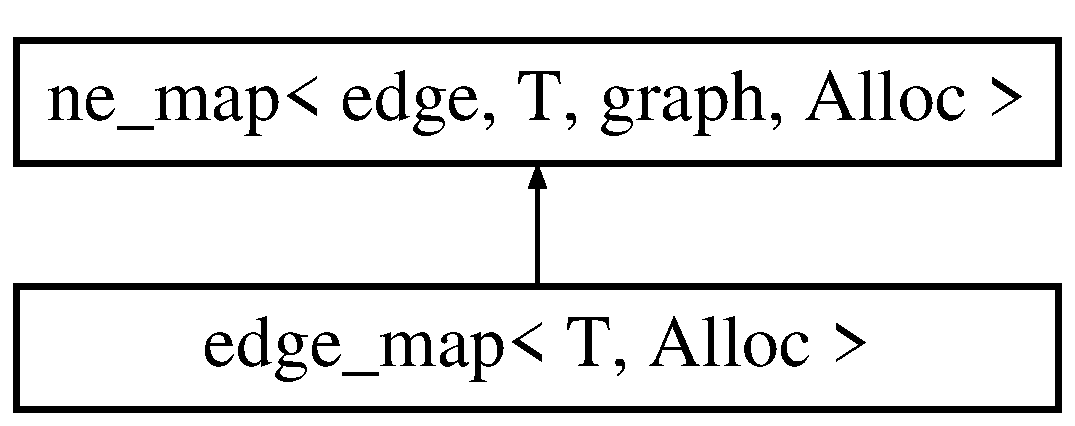
\includegraphics[height=2.000000cm]{classedge__map}
\end{center}
\end{figure}
\subsection*{Public Member Functions}
\begin{DoxyCompactItemize}
\item 
\mbox{\hyperlink{classedge__map_a947fa280ba03fd11b1813d484572e6df}{edge\+\_\+map}} ()
\item 
\mbox{\hyperlink{classedge__map_a30bd07fe13081b22071b721f66bb6796}{edge\+\_\+map}} (const \mbox{\hyperlink{classgraph}{graph}} \&g, T t=T())
\end{DoxyCompactItemize}
\subsection*{Additional Inherited Members}


\subsection{Detailed Description}
\subsubsection*{template$<$class T, class Alloc = allocator$<$\+T$>$$>$\newline
class edge\+\_\+map$<$ T, Alloc $>$}

A specialized map with edges as keys. 

A {\ttfamily \mbox{\hyperlink{classedge__map}{edge\+\_\+map}}} is a specialized and optimized map implementation with edges as keys. Using a {\ttfamily \mbox{\hyperlink{classedge__map}{edge\+\_\+map}}} is the standard way to attach user defined information to the edges of a {\ttfamily graph}.

An example of usage\+: 
\begin{DoxyPre}
  graph g;\end{DoxyPre}



\begin{DoxyPre}  node v1 = g.new\_node();
  node v2 = g.new\_node();
  edge e = g.new\_edge(v1, v2);\end{DoxyPre}



\begin{DoxyPre}  \mbox{\hyperlink{classedge__map}{edge\_map}}<string> label(g, "Default Label");\end{DoxyPre}



\begin{DoxyPre}  label[e] = "An edge";\end{DoxyPre}



\begin{DoxyPre}  assert(label[e] == "An edge");
\end{DoxyPre}


The edges used as keys for a {\ttfamily \mbox{\hyperlink{classedge__map}{edge\+\_\+map}}} M\+U\+ST be edges of the same graph. If you want to use edges from different graphs, use a {\ttfamily map$<$edge,T$>$} instead. A graph and a copy of it are considered to be different.

Most of the functionality of {\ttfamily \mbox{\hyperlink{classedge__map}{edge\+\_\+map}}} is inherited from \mbox{\hyperlink{classne__map}{ne\+\_\+map}}.

\begin{DoxySeeAlso}{See also}
\mbox{\hyperlink{classnode__map}{node\+\_\+map}} 
\end{DoxySeeAlso}


\subsection{Constructor \& Destructor Documentation}
\mbox{\Hypertarget{classedge__map_a947fa280ba03fd11b1813d484572e6df}\label{classedge__map_a947fa280ba03fd11b1813d484572e6df}} 
\index{edge\+\_\+map@{edge\+\_\+map}!edge\+\_\+map@{edge\+\_\+map}}
\index{edge\+\_\+map@{edge\+\_\+map}!edge\+\_\+map@{edge\+\_\+map}}
\subsubsection{\texorpdfstring{edge\+\_\+map()}{edge\_map()}\hspace{0.1cm}{\footnotesize\ttfamily [1/2]}}
{\footnotesize\ttfamily template$<$class T, class Alloc = allocator$<$\+T$>$$>$ \\
\mbox{\hyperlink{classedge__map}{edge\+\_\+map}}$<$ T, Alloc $>$\+::\mbox{\hyperlink{classedge__map}{edge\+\_\+map}} (\begin{DoxyParamCaption}{ }\end{DoxyParamCaption})\hspace{0.3cm}{\ttfamily [inline]}}

Constructs an empty {\ttfamily \mbox{\hyperlink{classedge__map}{edge\+\_\+map}}} not associated with any {\ttfamily graph}. You may (but need not) call {\ttfamily ne\+\_\+map\+::init(const graph \&, T)} to associate it to a {\ttfamily graph}. \mbox{\Hypertarget{classedge__map_a30bd07fe13081b22071b721f66bb6796}\label{classedge__map_a30bd07fe13081b22071b721f66bb6796}} 
\index{edge\+\_\+map@{edge\+\_\+map}!edge\+\_\+map@{edge\+\_\+map}}
\index{edge\+\_\+map@{edge\+\_\+map}!edge\+\_\+map@{edge\+\_\+map}}
\subsubsection{\texorpdfstring{edge\+\_\+map()}{edge\_map()}\hspace{0.1cm}{\footnotesize\ttfamily [2/2]}}
{\footnotesize\ttfamily template$<$class T, class Alloc = allocator$<$\+T$>$$>$ \\
\mbox{\hyperlink{classedge__map}{edge\+\_\+map}}$<$ T, Alloc $>$\+::\mbox{\hyperlink{classedge__map}{edge\+\_\+map}} (\begin{DoxyParamCaption}\item[{const \mbox{\hyperlink{classgraph}{graph}} \&}]{g,  }\item[{T}]{t = {\ttfamily T()} }\end{DoxyParamCaption})\hspace{0.3cm}{\ttfamily [inline]}, {\ttfamily [explicit]}}

Constructs a {\ttfamily \mbox{\hyperlink{classedge__map}{edge\+\_\+map}}} associated to the graph {\ttfamily g}. The value associated to each edge in {\ttfamily g} is set to {\ttfamily t}. 

The documentation for this class was generated from the following file\+:\begin{DoxyCompactItemize}
\item 
include/\+K\+G\+L/edge\+\_\+map.\+h\end{DoxyCompactItemize}

\hypertarget{classfm__partition}{}\section{fm\+\_\+partition Class Reference}
\label{classfm__partition}\index{fm\+\_\+partition@{fm\+\_\+partition}}


Heuristic graph bi-\/partitioning algorithm (Fiduccia-\/\+Mattheyses).  




{\ttfamily \#include $<$fm\+\_\+partition.\+h$>$}

Inheritance diagram for fm\+\_\+partition\+:\begin{figure}[H]
\begin{center}
\leavevmode
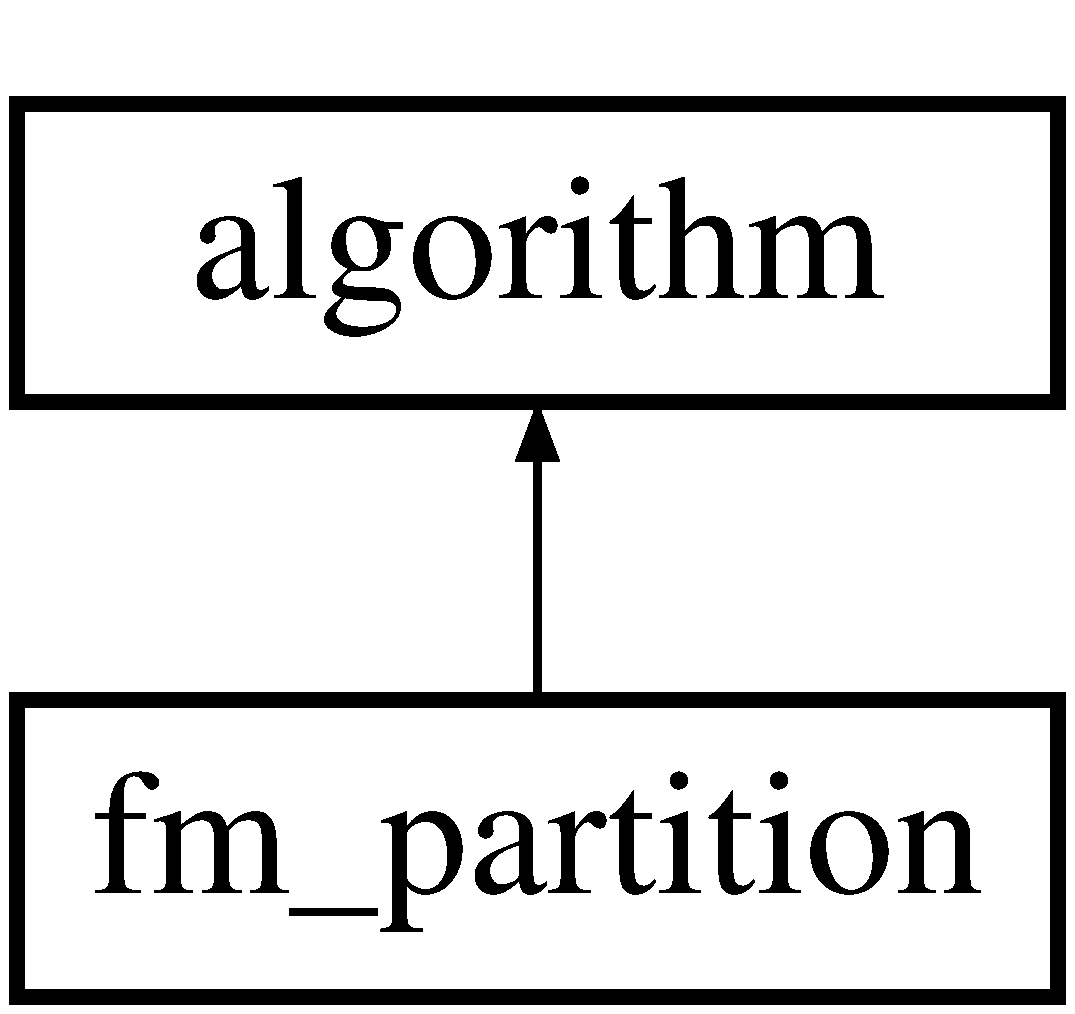
\includegraphics[height=2.000000cm]{classfm__partition}
\end{center}
\end{figure}
\subsection*{Public Types}
\begin{DoxyCompactItemize}
\item 
typedef int \mbox{\hyperlink{classfm__partition_a7cdff1bea3740a287387e8408e16ca79}{side\+\_\+type}}
\item 
typedef short int \mbox{\hyperlink{classfm__partition_a63693cd93d587dca3d1842f831cd1c55}{fix\+\_\+type}}
\item 
typedef list$<$ \mbox{\hyperlink{classedge}{edge}} $>$\+::const\+\_\+iterator \mbox{\hyperlink{classfm__partition_aede10aea3dda6be8014ce60fca728efe}{cut\+\_\+edges\+\_\+iterator}}
\item 
typedef list$<$ \mbox{\hyperlink{classnode}{node}} $>$\+::const\+\_\+iterator \mbox{\hyperlink{classfm__partition_ac8b7b5253476118e5f7bbad2fe8af285}{nodes\+\_\+of\+\_\+one\+\_\+side\+\_\+iterator}}
\end{DoxyCompactItemize}
\subsection*{Public Member Functions}
\begin{DoxyCompactItemize}
\item 
\mbox{\hyperlink{classfm__partition_a69f37c22abf6df5b3778623512240106}{fm\+\_\+partition}} ()
\item 
virtual \mbox{\hyperlink{classfm__partition_ab9d4f12de8f65d42240d94f7924fb319}{$\sim$fm\+\_\+partition}} ()
\item 
void \mbox{\hyperlink{classfm__partition_aa15471da2b6a0f14060b0c4091c6b05c}{set\+\_\+vars}} (const \mbox{\hyperlink{classgraph}{graph}} \&G, const \mbox{\hyperlink{classnode__map}{node\+\_\+map}}$<$ int $>$ \&node\+\_\+weight, const \mbox{\hyperlink{classedge__map}{edge\+\_\+map}}$<$ int $>$ \&edge\+\_\+weight)
\item 
void \mbox{\hyperlink{classfm__partition_af4d1b1275050cc7f4327500cec1f6e88}{set\+\_\+vars}} (const \mbox{\hyperlink{classgraph}{graph}} \&G, const \mbox{\hyperlink{classnode__map}{node\+\_\+map}}$<$ int $>$ \&node\+\_\+weight, const \mbox{\hyperlink{classedge__map}{edge\+\_\+map}}$<$ int $>$ \&edge\+\_\+weight, const \mbox{\hyperlink{classnode__map}{node\+\_\+map}}$<$ \mbox{\hyperlink{classfm__partition_a7cdff1bea3740a287387e8408e16ca79}{side\+\_\+type}} $>$ \&init\+\_\+side)
\item 
void \mbox{\hyperlink{classfm__partition_ad0bebf48731e99fbf7a8c6526ab0f9a6}{set\+\_\+vars}} (const \mbox{\hyperlink{classgraph}{graph}} \&G, const \mbox{\hyperlink{classnode__map}{node\+\_\+map}}$<$ int $>$ \&node\+\_\+weight, const \mbox{\hyperlink{classedge__map}{edge\+\_\+map}}$<$ int $>$ \&edge\+\_\+weight, const \mbox{\hyperlink{classnode__map}{node\+\_\+map}}$<$ \mbox{\hyperlink{classfm__partition_a63693cd93d587dca3d1842f831cd1c55}{fix\+\_\+type}} $>$ \&fixed)
\item 
void \mbox{\hyperlink{classfm__partition_a19ade0d3e19eb40841238c1048c4495b}{set\+\_\+vars}} (const \mbox{\hyperlink{classgraph}{graph}} \&G, const \mbox{\hyperlink{classnode__map}{node\+\_\+map}}$<$ int $>$ \&node\+\_\+weight, const \mbox{\hyperlink{classedge__map}{edge\+\_\+map}}$<$ int $>$ \&edge\+\_\+weight, const \mbox{\hyperlink{classnode__map}{node\+\_\+map}}$<$ \mbox{\hyperlink{classfm__partition_a7cdff1bea3740a287387e8408e16ca79}{side\+\_\+type}} $>$ \&init\+\_\+side, const \mbox{\hyperlink{classnode__map}{node\+\_\+map}}$<$ \mbox{\hyperlink{classfm__partition_a63693cd93d587dca3d1842f831cd1c55}{fix\+\_\+type}} $>$ \&fixed)
\item 
void \mbox{\hyperlink{classfm__partition_ad0870674a1fb8e1c882f6855e32aec09}{store\+\_\+cut\+\_\+edges}} (const bool set)
\item 
void \mbox{\hyperlink{classfm__partition_a8926005b4637055d2acf6f29ad2d9b97}{store\+\_\+nodes\+AB}} (const bool set)
\item 
virtual auto \+\_\+\+\_\+cdecl \mbox{\hyperlink{classfm__partition_a2fadbf126742f659878132159653e102}{check}} (\mbox{\hyperlink{classgraph}{graph}} \&G) -\/$>$ int
\item 
auto \+\_\+\+\_\+cdecl \mbox{\hyperlink{classfm__partition_a509615ef1f11bc2334a96c35adafd28e}{run}} (\mbox{\hyperlink{classgraph}{graph}} \&G) -\/$>$ int
\item 
int \mbox{\hyperlink{classfm__partition_a42fa2e19fb3fde093a1a05d0bd6d8ad1}{get\+\_\+cutsize}} ()
\item 
int \mbox{\hyperlink{classfm__partition_aa8aa84286a6939d17175fbf646ba3176}{get\+\_\+needed\+\_\+passes}} ()
\item 
\mbox{\hyperlink{classfm__partition_a7cdff1bea3740a287387e8408e16ca79}{side\+\_\+type}} \mbox{\hyperlink{classfm__partition_af5f6ad817fe30760f3bc5470bd70c4c9}{get\+\_\+side\+\_\+of\+\_\+node}} (const \mbox{\hyperlink{classnode}{node}} \&n) const
\item 
\mbox{\hyperlink{classfm__partition_a7cdff1bea3740a287387e8408e16ca79}{side\+\_\+type}} \mbox{\hyperlink{classfm__partition_a45ef6bc577ce894ead2c699678e26f1b}{operator\mbox{[}$\,$\mbox{]}}} (const \mbox{\hyperlink{classnode}{node}} \&n) const
\item 
int \mbox{\hyperlink{classfm__partition_a3f1ddcff1ba7a4c4090f947f918b5331}{get\+\_\+weight\+\_\+on\+\_\+sideA}} (const \mbox{\hyperlink{classgraph}{graph}} \&G) const
\item 
int \mbox{\hyperlink{classfm__partition_a9e380da1dc654fcffdf4ac2418c6ef80}{get\+\_\+weight\+\_\+on\+\_\+sideB}} (const \mbox{\hyperlink{classgraph}{graph}} \&G) const
\item 
\mbox{\hyperlink{classfm__partition_aede10aea3dda6be8014ce60fca728efe}{cut\+\_\+edges\+\_\+iterator}} \mbox{\hyperlink{classfm__partition_a36990b62c6d2d9e4948f42d805afc626}{cut\+\_\+edges\+\_\+begin}} () const
\item 
\mbox{\hyperlink{classfm__partition_aede10aea3dda6be8014ce60fca728efe}{cut\+\_\+edges\+\_\+iterator}} \mbox{\hyperlink{classfm__partition_af213672f08e03878183659fa8c2ed61e}{cut\+\_\+edges\+\_\+end}} () const
\item 
\mbox{\hyperlink{classfm__partition_ac8b7b5253476118e5f7bbad2fe8af285}{nodes\+\_\+of\+\_\+one\+\_\+side\+\_\+iterator}} \mbox{\hyperlink{classfm__partition_adad3bf33efb4a2b1b0feadeafb33f5fd}{nodes\+\_\+of\+\_\+side\+A\+\_\+begin}} () const
\item 
\mbox{\hyperlink{classfm__partition_ac8b7b5253476118e5f7bbad2fe8af285}{nodes\+\_\+of\+\_\+one\+\_\+side\+\_\+iterator}} \mbox{\hyperlink{classfm__partition_ac4202d1d929c1700985ad5d452b735fb}{nodes\+\_\+of\+\_\+side\+A\+\_\+end}} () const
\item 
\mbox{\hyperlink{classfm__partition_ac8b7b5253476118e5f7bbad2fe8af285}{nodes\+\_\+of\+\_\+one\+\_\+side\+\_\+iterator}} \mbox{\hyperlink{classfm__partition_a4e433456ed0214c04466c4f1060b0909}{nodes\+\_\+of\+\_\+side\+B\+\_\+begin}} () const
\item 
\mbox{\hyperlink{classfm__partition_ac8b7b5253476118e5f7bbad2fe8af285}{nodes\+\_\+of\+\_\+one\+\_\+side\+\_\+iterator}} \mbox{\hyperlink{classfm__partition_a9682b070cce104bdfe69e576df57f560}{nodes\+\_\+of\+\_\+side\+B\+\_\+end}} () const
\item 
virtual auto \+\_\+\+\_\+cdecl \mbox{\hyperlink{classfm__partition_a05ba0de86d7fe9c2de81b0681d8e0102}{reset}} () -\/$>$ void
\end{DoxyCompactItemize}
\subsection*{Static Public Attributes}
\begin{DoxyCompactItemize}
\item 
static const \mbox{\hyperlink{classfm__partition_a7cdff1bea3740a287387e8408e16ca79}{side\+\_\+type}} \mbox{\hyperlink{classfm__partition_a973d30e9eb0d21f659ef288176cd4791}{A}} = 0
\item 
static const \mbox{\hyperlink{classfm__partition_a7cdff1bea3740a287387e8408e16ca79}{side\+\_\+type}} \mbox{\hyperlink{classfm__partition_a42515c44eecb7ba3e2ec549a877ef238}{B}} = 1
\item 
static const \mbox{\hyperlink{classfm__partition_a63693cd93d587dca3d1842f831cd1c55}{fix\+\_\+type}} \mbox{\hyperlink{classfm__partition_a468a80e072d3ff18e5da33005825bcb1}{F\+I\+XA}} = 0
\item 
static const \mbox{\hyperlink{classfm__partition_a63693cd93d587dca3d1842f831cd1c55}{fix\+\_\+type}} \mbox{\hyperlink{classfm__partition_a0b9a66f0e8093ee83482f93d6aa5b2eb}{F\+I\+XB}} = 1
\item 
static const \mbox{\hyperlink{classfm__partition_a63693cd93d587dca3d1842f831cd1c55}{fix\+\_\+type}} \mbox{\hyperlink{classfm__partition_a24447561db0ea633212c597c5e1fca56}{U\+N\+F\+I\+X\+ED}} = 2
\end{DoxyCompactItemize}
\subsection*{Protected Member Functions}
\begin{DoxyCompactItemize}
\item 
\mbox{\Hypertarget{classfm__partition_ad768579b813500dc2d267aac5668ed48}\label{classfm__partition_ad768579b813500dc2d267aac5668ed48}} 
void {\bfseries divide\+\_\+up} (const \mbox{\hyperlink{classgraph}{graph}} \&G)
\item 
\mbox{\Hypertarget{classfm__partition_a3e3aa22119ff5ff9c406683e22ab6078}\label{classfm__partition_a3e3aa22119ff5ff9c406683e22ab6078}} 
void {\bfseries hide\+\_\+self\+\_\+loops} (\mbox{\hyperlink{classgraph}{graph}} \&G)
\item 
\mbox{\Hypertarget{classfm__partition_aad791ac648a9ff4694c8960f49dcc018}\label{classfm__partition_aad791ac648a9ff4694c8960f49dcc018}} 
void {\bfseries init\+\_\+variables} (const \mbox{\hyperlink{classgraph}{graph}} \&G)
\item 
\mbox{\Hypertarget{classfm__partition_a25ef3fc22bee176abfef64248484e8c0}\label{classfm__partition_a25ef3fc22bee176abfef64248484e8c0}} 
void {\bfseries create\+\_\+initial\+\_\+bipart} (const \mbox{\hyperlink{classgraph}{graph}} \&G)
\item 
\mbox{\Hypertarget{classfm__partition_a2118f4ef46c76ed9863ee8c9cd557a09}\label{classfm__partition_a2118f4ef46c76ed9863ee8c9cd557a09}} 
void {\bfseries shuffle\+\_\+vector} (const int vector\+\_\+size, vector$<$ graph\+::node\+\_\+iterator $>$ \&node\+\_\+vector)
\item 
\mbox{\Hypertarget{classfm__partition_a5d0f409b6b1d554a62d67952236c7ce9}\label{classfm__partition_a5d0f409b6b1d554a62d67952236c7ce9}} 
void {\bfseries compute\+\_\+max\+\_\+vertex\+\_\+degree} (const \mbox{\hyperlink{classgraph}{graph}} \&G)
\item 
\mbox{\Hypertarget{classfm__partition_aec7b2a315bc003fbd98debd5cd879f99}\label{classfm__partition_aec7b2a315bc003fbd98debd5cd879f99}} 
void {\bfseries pass\+\_\+manager} (const \mbox{\hyperlink{classgraph}{graph}} \&G)
\item 
\mbox{\Hypertarget{classfm__partition_a33d1dbba0ce9e398adab753f403deac3}\label{classfm__partition_a33d1dbba0ce9e398adab753f403deac3}} 
void {\bfseries copy\+\_\+side\+\_\+node\+\_\+map} (const \mbox{\hyperlink{classgraph}{graph}} \&G, \mbox{\hyperlink{classnode__map}{node\+\_\+map}}$<$ \mbox{\hyperlink{classfm__partition_a7cdff1bea3740a287387e8408e16ca79}{side\+\_\+type}} $>$ \&dest, const \mbox{\hyperlink{classnode__map}{node\+\_\+map}}$<$ \mbox{\hyperlink{classfm__partition_a7cdff1bea3740a287387e8408e16ca79}{side\+\_\+type}} $>$ source) const
\item 
\mbox{\Hypertarget{classfm__partition_a9aa27d4c97616c0fdbd00d11dc83bc0b}\label{classfm__partition_a9aa27d4c97616c0fdbd00d11dc83bc0b}} 
void {\bfseries init\+\_\+data\+\_\+structure} (const \mbox{\hyperlink{classgraph}{graph}} \&G)
\item 
\mbox{\Hypertarget{classfm__partition_ac510befe1837c646a260a14c110d7a79}\label{classfm__partition_ac510befe1837c646a260a14c110d7a79}} 
void {\bfseries init\+\_\+filling\+\_\+buckets} (const \mbox{\hyperlink{classgraph}{graph}} \&G)
\item 
\mbox{\Hypertarget{classfm__partition_a50c61b9d27e83a98e2e04a47b51670b6}\label{classfm__partition_a50c61b9d27e83a98e2e04a47b51670b6}} 
int {\bfseries inital\+\_\+gain\+\_\+of\+\_\+node\+\_\+on\+\_\+sideA} (const \mbox{\hyperlink{classnode}{node}} cur\+\_\+node)
\item 
\mbox{\Hypertarget{classfm__partition_aa217da6a3c8a736e9e51aa348c951501}\label{classfm__partition_aa217da6a3c8a736e9e51aa348c951501}} 
int {\bfseries inital\+\_\+gain\+\_\+of\+\_\+node\+\_\+on\+\_\+sideB} (const \mbox{\hyperlink{classnode}{node}} cur\+\_\+node)
\item 
\mbox{\Hypertarget{classfm__partition_a91572409b30f0967ea3782079f69b1bb}\label{classfm__partition_a91572409b30f0967ea3782079f69b1bb}} 
void {\bfseries move\+\_\+manager} (const \mbox{\hyperlink{classgraph}{graph}} \&G)
\item 
\mbox{\Hypertarget{classfm__partition_ac1167c6595a9f582ae98c9f555029d9b}\label{classfm__partition_ac1167c6595a9f582ae98c9f555029d9b}} 
bool {\bfseries move\+\_\+vertex} (const \mbox{\hyperlink{classgraph}{graph}} \&G, \mbox{\hyperlink{classnode}{node}} \&moved\+\_\+node)
\item 
\mbox{\Hypertarget{classfm__partition_a6dc702df474c4ce60e80b3e5a93b7f4d}\label{classfm__partition_a6dc702df474c4ce60e80b3e5a93b7f4d}} 
bool {\bfseries balance\+\_\+holds} (const \mbox{\hyperlink{classgraph}{graph}} \&G, const \mbox{\hyperlink{classnode}{node}} cur\+\_\+node)
\item 
\mbox{\Hypertarget{classfm__partition_a8bd7f2715334e9ec95da8001117fdde5}\label{classfm__partition_a8bd7f2715334e9ec95da8001117fdde5}} 
void {\bfseries update\+\_\+data\+\_\+structure\+\_\+\+A2B} (const \mbox{\hyperlink{classnode}{node}} cur\+\_\+node)
\item 
\mbox{\Hypertarget{classfm__partition_a783174f29d49e7e1ae7f6cf71faa82fb}\label{classfm__partition_a783174f29d49e7e1ae7f6cf71faa82fb}} 
void {\bfseries update\+\_\+data\+\_\+structure\+\_\+\+B2A} (const \mbox{\hyperlink{classnode}{node}} cur\+\_\+node)
\item 
\mbox{\Hypertarget{classfm__partition_aa4ec83c52916cc6cac23e7a9987427cd}\label{classfm__partition_aa4ec83c52916cc6cac23e7a9987427cd}} 
void {\bfseries update\+\_\+bucketA} (const \mbox{\hyperlink{classnode}{node}} cur\+\_\+node, const int old\+\_\+gain, const int new\+\_\+gain)
\item 
\mbox{\Hypertarget{classfm__partition_a270d469ca584ed9adff9fced67743679}\label{classfm__partition_a270d469ca584ed9adff9fced67743679}} 
void {\bfseries update\+\_\+bucketB} (const \mbox{\hyperlink{classnode}{node}} cur\+\_\+node, const int old\+\_\+gain, const int new\+\_\+gain)
\item 
\mbox{\Hypertarget{classfm__partition_a335722b73c1d6f02d1083e76a3937b01}\label{classfm__partition_a335722b73c1d6f02d1083e76a3937b01}} 
void {\bfseries update\+\_\+max\+\_\+gain} (const \mbox{\hyperlink{classfm__partition_a7cdff1bea3740a287387e8408e16ca79}{side\+\_\+type}} side)
\item 
\mbox{\Hypertarget{classfm__partition_ac49d477ecbf512fa375b76a472ec54f8}\label{classfm__partition_ac49d477ecbf512fa375b76a472ec54f8}} 
int {\bfseries range\+\_\+up} (const int gain\+\_\+value) const
\item 
\mbox{\Hypertarget{classfm__partition_ab0bfbda97056ac75ab5fbfa6fd20fd03}\label{classfm__partition_ab0bfbda97056ac75ab5fbfa6fd20fd03}} 
int {\bfseries range\+\_\+down} (const int index) const
\item 
\mbox{\Hypertarget{classfm__partition_a15197263e5318f824e0cde66ea9132b7}\label{classfm__partition_a15197263e5318f824e0cde66ea9132b7}} 
void {\bfseries clean\+\_\+pass} (const \mbox{\hyperlink{classgraph}{graph}} \&G)
\item 
\mbox{\Hypertarget{classfm__partition_a03c76998f985593caddc4979a28b9042}\label{classfm__partition_a03c76998f985593caddc4979a28b9042}} 
void {\bfseries compute\+\_\+cut\+\_\+edges} (const \mbox{\hyperlink{classgraph}{graph}} \&G)
\item 
\mbox{\Hypertarget{classfm__partition_aaa8f24af3be860bfa42a171c25420c2c}\label{classfm__partition_aaa8f24af3be860bfa42a171c25420c2c}} 
void {\bfseries compute\+\_\+nodes\+AB} (const \mbox{\hyperlink{classgraph}{graph}} \&G)
\end{DoxyCompactItemize}
\subsection*{Protected Attributes}
\begin{DoxyCompactItemize}
\item 
\mbox{\Hypertarget{classfm__partition_a806c9f5cb781b8ce662d2a3373433777}\label{classfm__partition_a806c9f5cb781b8ce662d2a3373433777}} 
bool {\bfseries enable\+\_\+cut\+\_\+edges\+\_\+storing}
\item 
\mbox{\Hypertarget{classfm__partition_abf5c178fa75d8d723cb7757da60321d6}\label{classfm__partition_abf5c178fa75d8d723cb7757da60321d6}} 
list$<$ \mbox{\hyperlink{classedge}{edge}} $>$ {\bfseries cut\+\_\+edges}
\item 
\mbox{\Hypertarget{classfm__partition_a2e308857dde9405bc3c6b911218bcda1}\label{classfm__partition_a2e308857dde9405bc3c6b911218bcda1}} 
bool {\bfseries enable\+\_\+nodes\+A\+B\+\_\+storing}
\item 
\mbox{\Hypertarget{classfm__partition_a3822e72fc18189cf64955edb33ece653}\label{classfm__partition_a3822e72fc18189cf64955edb33ece653}} 
list$<$ \mbox{\hyperlink{classnode}{node}} $>$ {\bfseries nodesA}
\item 
\mbox{\Hypertarget{classfm__partition_a60552f973cf9b30396c6505b72de4261}\label{classfm__partition_a60552f973cf9b30396c6505b72de4261}} 
list$<$ \mbox{\hyperlink{classnode}{node}} $>$ {\bfseries nodesB}
\item 
\mbox{\Hypertarget{classfm__partition_a58edb78c4da479cd790da1eed1a30eab}\label{classfm__partition_a58edb78c4da479cd790da1eed1a30eab}} 
bool {\bfseries set\+\_\+vars\+\_\+executed}
\item 
\mbox{\Hypertarget{classfm__partition_a38c67abb32d7ade03b68f0a7ed9f1c6d}\label{classfm__partition_a38c67abb32d7ade03b68f0a7ed9f1c6d}} 
bool {\bfseries provided\+\_\+initial\+\_\+part}
\item 
\mbox{\Hypertarget{classfm__partition_a0aca0fa4fcaba284d61c745d17022f8d}\label{classfm__partition_a0aca0fa4fcaba284d61c745d17022f8d}} 
bool {\bfseries provided\+\_\+fix}
\item 
\mbox{\Hypertarget{classfm__partition_a3b04658dbb5b27ddd20194ff74a71082}\label{classfm__partition_a3b04658dbb5b27ddd20194ff74a71082}} 
\mbox{\hyperlink{classnode__map}{node\+\_\+map}}$<$ \mbox{\hyperlink{classfm__partition_a63693cd93d587dca3d1842f831cd1c55}{fix\+\_\+type}} $>$ {\bfseries fixed}
\item 
\mbox{\Hypertarget{classfm__partition_ae1ba643b4bd6721075ab7b608bcf3cd6}\label{classfm__partition_ae1ba643b4bd6721075ab7b608bcf3cd6}} 
\mbox{\hyperlink{classnode__map}{node\+\_\+map}}$<$ int $>$ {\bfseries node\+\_\+weight}
\item 
\mbox{\Hypertarget{classfm__partition_a8591f5eddac01679e1da3d835eae1cf6}\label{classfm__partition_a8591f5eddac01679e1da3d835eae1cf6}} 
int {\bfseries max\+\_\+node\+\_\+weight}
\item 
\mbox{\Hypertarget{classfm__partition_adfe6147ba3f9c785f613b472f950595f}\label{classfm__partition_adfe6147ba3f9c785f613b472f950595f}} 
\mbox{\hyperlink{classedge__map}{edge\+\_\+map}}$<$ int $>$ {\bfseries edge\+\_\+weight}
\item 
\mbox{\Hypertarget{classfm__partition_a5b37b4ac8d96236f274a57a46d653e25}\label{classfm__partition_a5b37b4ac8d96236f274a57a46d653e25}} 
int {\bfseries max\+\_\+edge\+\_\+weight}
\item 
\mbox{\Hypertarget{classfm__partition_a25651e3f78ddbc418ea978ca6b28e0e0}\label{classfm__partition_a25651e3f78ddbc418ea978ca6b28e0e0}} 
int {\bfseries total\+\_\+node\+\_\+weight}
\item 
\mbox{\Hypertarget{classfm__partition_a8a50d15b399c9ed35d6987c8fb68aa2b}\label{classfm__partition_a8a50d15b399c9ed35d6987c8fb68aa2b}} 
int {\bfseries node\+\_\+weight\+\_\+on\+\_\+sideA}
\item 
\mbox{\Hypertarget{classfm__partition_a6dc967e385b31096a85f17c51f1f0824}\label{classfm__partition_a6dc967e385b31096a85f17c51f1f0824}} 
int {\bfseries node\+\_\+weight\+\_\+on\+\_\+sideB}
\item 
\mbox{\Hypertarget{classfm__partition_af83309e781e9658fc0ff923ced087bfc}\label{classfm__partition_af83309e781e9658fc0ff923ced087bfc}} 
\mbox{\hyperlink{classnode__map}{node\+\_\+map}}$<$ \mbox{\hyperlink{classfm__partition_a7cdff1bea3740a287387e8408e16ca79}{side\+\_\+type}} $>$ {\bfseries side}
\item 
\mbox{\Hypertarget{classfm__partition_a7cbed9aeba4dae80047b45849e61bfa5}\label{classfm__partition_a7cbed9aeba4dae80047b45849e61bfa5}} 
\mbox{\hyperlink{classnode__map}{node\+\_\+map}}$<$ list$<$ \mbox{\hyperlink{classnode}{node}} $>$\+::iterator $>$ {\bfseries position\+\_\+in\+\_\+bucket}
\item 
\mbox{\Hypertarget{classfm__partition_ab6a4beaa10548ce9f1a0e8e441492ef9}\label{classfm__partition_ab6a4beaa10548ce9f1a0e8e441492ef9}} 
int {\bfseries max\+\_\+vertex\+\_\+degree}
\item 
\mbox{\Hypertarget{classfm__partition_a14b0aa9a91a6e7fa3035669cf5056275}\label{classfm__partition_a14b0aa9a91a6e7fa3035669cf5056275}} 
\mbox{\hyperlink{classedge__map}{edge\+\_\+map}}$<$ int $>$ {\bfseries aside}
\item 
\mbox{\Hypertarget{classfm__partition_aa75765887173fb06b076b6cae12d4e66}\label{classfm__partition_aa75765887173fb06b076b6cae12d4e66}} 
\mbox{\hyperlink{classedge__map}{edge\+\_\+map}}$<$ int $>$ {\bfseries bside}
\item 
\mbox{\Hypertarget{classfm__partition_a7766d33d004b60c90a95220b2ada12e5}\label{classfm__partition_a7766d33d004b60c90a95220b2ada12e5}} 
\mbox{\hyperlink{classedge__map}{edge\+\_\+map}}$<$ list$<$ \mbox{\hyperlink{classnode}{node}} $>$ $>$ {\bfseries unlockedA}
\item 
\mbox{\Hypertarget{classfm__partition_a8ac9c48ade76692d385dc61fa3ba5f68}\label{classfm__partition_a8ac9c48ade76692d385dc61fa3ba5f68}} 
\mbox{\hyperlink{classedge__map}{edge\+\_\+map}}$<$ list$<$ \mbox{\hyperlink{classnode}{node}} $>$ $>$ {\bfseries unlockedB}
\item 
\mbox{\Hypertarget{classfm__partition_ae8176f4ce82305abfd58e519d2cdd91d}\label{classfm__partition_ae8176f4ce82305abfd58e519d2cdd91d}} 
\mbox{\hyperlink{classnode__map}{node\+\_\+map}}$<$ int $>$ {\bfseries gain\+\_\+value}
\item 
\mbox{\Hypertarget{classfm__partition_a4df2f0f6f4686ba187c2be39ce3b29cc}\label{classfm__partition_a4df2f0f6f4686ba187c2be39ce3b29cc}} 
bool {\bfseries bucket\+A\+\_\+empty}
\item 
\mbox{\Hypertarget{classfm__partition_aef7d0f91cb7c04b4f5b1b14cc9884c37}\label{classfm__partition_aef7d0f91cb7c04b4f5b1b14cc9884c37}} 
bool {\bfseries bucket\+B\+\_\+empty}
\item 
\mbox{\Hypertarget{classfm__partition_a6c6a7a05bebe943e681329d30bb13339}\label{classfm__partition_a6c6a7a05bebe943e681329d30bb13339}} 
int {\bfseries max\+\_\+gainA}
\item 
\mbox{\Hypertarget{classfm__partition_ac230f89828768eaf51374c0bc3b37558}\label{classfm__partition_ac230f89828768eaf51374c0bc3b37558}} 
int {\bfseries max\+\_\+gainB}
\item 
\mbox{\Hypertarget{classfm__partition_ad12e34fc6babe6b4796fb0e5811c844e}\label{classfm__partition_ad12e34fc6babe6b4796fb0e5811c844e}} 
vector$<$ list$<$ \mbox{\hyperlink{classnode}{node}} $>$ $>$ {\bfseries bucketA}
\item 
\mbox{\Hypertarget{classfm__partition_a4c256551909261b6a5bcdaecd2637ba2}\label{classfm__partition_a4c256551909261b6a5bcdaecd2637ba2}} 
vector$<$ list$<$ \mbox{\hyperlink{classnode}{node}} $>$ $>$ {\bfseries bucketB}
\item 
\mbox{\Hypertarget{classfm__partition_abc8f24c354d2a15f8ec8ef9a46252c93}\label{classfm__partition_abc8f24c354d2a15f8ec8ef9a46252c93}} 
int {\bfseries cur\+\_\+cutsize}
\item 
\mbox{\Hypertarget{classfm__partition_af35277f499ad76a979ee33b0cd388dc5}\label{classfm__partition_af35277f499ad76a979ee33b0cd388dc5}} 
int {\bfseries no\+\_\+passes}
\end{DoxyCompactItemize}


\subsection{Detailed Description}
Heuristic graph bi-\/partitioning algorithm (Fiduccia-\/\+Mattheyses). 

This class implements a heuristic graph bi-\/partitioning algorithm, based on iterative movement, proposed by C. M. Fiduccia and R. M. Mattheyses in 1982.

In the case E is the set of edges of the graph, the algorithm needs {\ttfamily O($\vert$\+E$\vert$)} time to proceed.

\begin{DoxySeeAlso}{See also}
\mbox{\hyperlink{classratio__cut__partition}{ratio\+\_\+cut\+\_\+partition}} 
\end{DoxySeeAlso}


\subsection{Member Typedef Documentation}
\mbox{\Hypertarget{classfm__partition_aede10aea3dda6be8014ce60fca728efe}\label{classfm__partition_aede10aea3dda6be8014ce60fca728efe}} 
\index{fm\+\_\+partition@{fm\+\_\+partition}!cut\+\_\+edges\+\_\+iterator@{cut\+\_\+edges\+\_\+iterator}}
\index{cut\+\_\+edges\+\_\+iterator@{cut\+\_\+edges\+\_\+iterator}!fm\+\_\+partition@{fm\+\_\+partition}}
\subsubsection{\texorpdfstring{cut\+\_\+edges\+\_\+iterator}{cut\_edges\_iterator}}
{\footnotesize\ttfamily typedef list$<$\mbox{\hyperlink{classedge}{edge}}$>$\+::const\+\_\+iterator \mbox{\hyperlink{classfm__partition_aede10aea3dda6be8014ce60fca728efe}{fm\+\_\+partition\+::cut\+\_\+edges\+\_\+iterator}}}

Iterator type for edges which belong to the cut. \mbox{\Hypertarget{classfm__partition_a63693cd93d587dca3d1842f831cd1c55}\label{classfm__partition_a63693cd93d587dca3d1842f831cd1c55}} 
\index{fm\+\_\+partition@{fm\+\_\+partition}!fix\+\_\+type@{fix\+\_\+type}}
\index{fix\+\_\+type@{fix\+\_\+type}!fm\+\_\+partition@{fm\+\_\+partition}}
\subsubsection{\texorpdfstring{fix\+\_\+type}{fix\_type}}
{\footnotesize\ttfamily typedef short int \mbox{\hyperlink{classfm__partition_a63693cd93d587dca3d1842f831cd1c55}{fm\+\_\+partition\+::fix\+\_\+type}}}

Fix type of each node (needed with \mbox{\hyperlink{classfm__partition_aa15471da2b6a0f14060b0c4091c6b05c}{fm\+\_\+partition\+::set\+\_\+vars}}).

\begin{DoxySeeAlso}{See also}
\mbox{\hyperlink{classfm__partition_a468a80e072d3ff18e5da33005825bcb1}{fm\+\_\+partition\+::\+F\+I\+XA}} 

\mbox{\hyperlink{classfm__partition_a0b9a66f0e8093ee83482f93d6aa5b2eb}{fm\+\_\+partition\+::\+F\+I\+XB}} 

\mbox{\hyperlink{classfm__partition_a24447561db0ea633212c597c5e1fca56}{fm\+\_\+partition\+::\+U\+N\+F\+I\+X\+ED}} 
\end{DoxySeeAlso}
\mbox{\Hypertarget{classfm__partition_ac8b7b5253476118e5f7bbad2fe8af285}\label{classfm__partition_ac8b7b5253476118e5f7bbad2fe8af285}} 
\index{fm\+\_\+partition@{fm\+\_\+partition}!nodes\+\_\+of\+\_\+one\+\_\+side\+\_\+iterator@{nodes\+\_\+of\+\_\+one\+\_\+side\+\_\+iterator}}
\index{nodes\+\_\+of\+\_\+one\+\_\+side\+\_\+iterator@{nodes\+\_\+of\+\_\+one\+\_\+side\+\_\+iterator}!fm\+\_\+partition@{fm\+\_\+partition}}
\subsubsection{\texorpdfstring{nodes\+\_\+of\+\_\+one\+\_\+side\+\_\+iterator}{nodes\_of\_one\_side\_iterator}}
{\footnotesize\ttfamily typedef list$<$\mbox{\hyperlink{classnode}{node}}$>$\+::const\+\_\+iterator \mbox{\hyperlink{classfm__partition_ac8b7b5253476118e5f7bbad2fe8af285}{fm\+\_\+partition\+::nodes\+\_\+of\+\_\+one\+\_\+side\+\_\+iterator}}}

Iterator type of nodes of a side. \mbox{\Hypertarget{classfm__partition_a7cdff1bea3740a287387e8408e16ca79}\label{classfm__partition_a7cdff1bea3740a287387e8408e16ca79}} 
\index{fm\+\_\+partition@{fm\+\_\+partition}!side\+\_\+type@{side\+\_\+type}}
\index{side\+\_\+type@{side\+\_\+type}!fm\+\_\+partition@{fm\+\_\+partition}}
\subsubsection{\texorpdfstring{side\+\_\+type}{side\_type}}
{\footnotesize\ttfamily typedef int \mbox{\hyperlink{classfm__partition_a7cdff1bea3740a287387e8408e16ca79}{fm\+\_\+partition\+::side\+\_\+type}}}

Return type of \mbox{\hyperlink{classfm__partition_af5f6ad817fe30760f3bc5470bd70c4c9}{fm\+\_\+partition\+::get\+\_\+side\+\_\+of\+\_\+node}}.

\begin{DoxySeeAlso}{See also}
\mbox{\hyperlink{classfm__partition_a973d30e9eb0d21f659ef288176cd4791}{fm\+\_\+partition\+::A}} 

\mbox{\hyperlink{classfm__partition_a42515c44eecb7ba3e2ec549a877ef238}{fm\+\_\+partition\+::B}} 
\end{DoxySeeAlso}


\subsection{Constructor \& Destructor Documentation}
\mbox{\Hypertarget{classfm__partition_a69f37c22abf6df5b3778623512240106}\label{classfm__partition_a69f37c22abf6df5b3778623512240106}} 
\index{fm\+\_\+partition@{fm\+\_\+partition}!fm\+\_\+partition@{fm\+\_\+partition}}
\index{fm\+\_\+partition@{fm\+\_\+partition}!fm\+\_\+partition@{fm\+\_\+partition}}
\subsubsection{\texorpdfstring{fm\+\_\+partition()}{fm\_partition()}}
{\footnotesize\ttfamily fm\+\_\+partition\+::fm\+\_\+partition (\begin{DoxyParamCaption}{ }\end{DoxyParamCaption})}

Default constructor.

\begin{DoxySeeAlso}{See also}
fm\+\_\+partition\+::fixe\+\_\+type 
\end{DoxySeeAlso}
\mbox{\Hypertarget{classfm__partition_ab9d4f12de8f65d42240d94f7924fb319}\label{classfm__partition_ab9d4f12de8f65d42240d94f7924fb319}} 
\index{fm\+\_\+partition@{fm\+\_\+partition}!````~fm\+\_\+partition@{$\sim$fm\+\_\+partition}}
\index{````~fm\+\_\+partition@{$\sim$fm\+\_\+partition}!fm\+\_\+partition@{fm\+\_\+partition}}
\subsubsection{\texorpdfstring{$\sim$fm\+\_\+partition()}{~fm\_partition()}}
{\footnotesize\ttfamily fm\+\_\+partition\+::$\sim$fm\+\_\+partition (\begin{DoxyParamCaption}{ }\end{DoxyParamCaption})\hspace{0.3cm}{\ttfamily [virtual]}}

Destructor.

\begin{DoxySeeAlso}{See also}
\mbox{\hyperlink{classalgorithm_adca9b1e7fa3afd914519a9dbb44e9fd5}{algorithm\+::$\sim$algorithm}} 
\end{DoxySeeAlso}


\subsection{Member Function Documentation}
\mbox{\Hypertarget{classfm__partition_a2fadbf126742f659878132159653e102}\label{classfm__partition_a2fadbf126742f659878132159653e102}} 
\index{fm\+\_\+partition@{fm\+\_\+partition}!check@{check}}
\index{check@{check}!fm\+\_\+partition@{fm\+\_\+partition}}
\subsubsection{\texorpdfstring{check()}{check()}}
{\footnotesize\ttfamily int fm\+\_\+partition\+::check (\begin{DoxyParamCaption}\item[{\mbox{\hyperlink{classgraph}{graph}} \&}]{G }\end{DoxyParamCaption}) -\/$>$ int\hspace{0.3cm}{\ttfamily [virtual]}}

Checks whether following preconditions are satisfied\+: 
\begin{DoxyItemize}
\item \mbox{\hyperlink{classfm__partition_aa15471da2b6a0f14060b0c4091c6b05c}{fm\+\_\+partition\+::set\+\_\+vars}} has been executed before. 
\item graph {\ttfamily G} is undirected. 
\item only node\+\_\+weights $>$= 0 are applied. 
\item only edge\+\_\+weights $>$= 0 are applied. 
\end{DoxyItemize}


\begin{DoxyParams}{Parameters}
{\em G} & graph \\
\hline
\end{DoxyParams}
\begin{DoxyReturn}{Returns}
{\ttfamily \mbox{\hyperlink{classalgorithm_af1a0078e153aa99c24f9bdf0d97f6710aae4c1cd7fe8d8cf4b143241a6e7c31cf}{algorithm\+::\+K\+G\+L\+\_\+\+OK}}} on success, {\ttfamily \mbox{\hyperlink{classalgorithm_af1a0078e153aa99c24f9bdf0d97f6710ae67bf27b2ef31f73e545a7f9f4a69556}{algorithm\+::\+K\+G\+L\+\_\+\+E\+R\+R\+OR}}} otherwise 
\end{DoxyReturn}
\begin{DoxySeeAlso}{See also}
\mbox{\hyperlink{classfm__partition_aa15471da2b6a0f14060b0c4091c6b05c}{fm\+\_\+partition\+::set\+\_\+vars}} 

\mbox{\hyperlink{classalgorithm_a05c0f25463eb35a77b2d73fc06bb2c0e}{algorithm\+::check}} 
\end{DoxySeeAlso}


Implements \mbox{\hyperlink{classalgorithm_a05c0f25463eb35a77b2d73fc06bb2c0e}{algorithm}}.

\mbox{\Hypertarget{classfm__partition_a36990b62c6d2d9e4948f42d805afc626}\label{classfm__partition_a36990b62c6d2d9e4948f42d805afc626}} 
\index{fm\+\_\+partition@{fm\+\_\+partition}!cut\+\_\+edges\+\_\+begin@{cut\+\_\+edges\+\_\+begin}}
\index{cut\+\_\+edges\+\_\+begin@{cut\+\_\+edges\+\_\+begin}!fm\+\_\+partition@{fm\+\_\+partition}}
\subsubsection{\texorpdfstring{cut\+\_\+edges\+\_\+begin()}{cut\_edges\_begin()}}
{\footnotesize\ttfamily \mbox{\hyperlink{classfm__partition_aede10aea3dda6be8014ce60fca728efe}{fm\+\_\+partition\+::cut\+\_\+edges\+\_\+iterator}} fm\+\_\+partition\+::cut\+\_\+edges\+\_\+begin (\begin{DoxyParamCaption}{ }\end{DoxyParamCaption}) const}

Iterate through all edges which belong to the cut, that means all edges with end-\/nodes on different sides. It is only valid if enabled with \mbox{\hyperlink{classfm__partition_ad0870674a1fb8e1c882f6855e32aec09}{fm\+\_\+partition\+::store\+\_\+cut\+\_\+edges}} before.

\begin{DoxyReturn}{Returns}
start for iteration through all cut edges 
\end{DoxyReturn}
\mbox{\Hypertarget{classfm__partition_af213672f08e03878183659fa8c2ed61e}\label{classfm__partition_af213672f08e03878183659fa8c2ed61e}} 
\index{fm\+\_\+partition@{fm\+\_\+partition}!cut\+\_\+edges\+\_\+end@{cut\+\_\+edges\+\_\+end}}
\index{cut\+\_\+edges\+\_\+end@{cut\+\_\+edges\+\_\+end}!fm\+\_\+partition@{fm\+\_\+partition}}
\subsubsection{\texorpdfstring{cut\+\_\+edges\+\_\+end()}{cut\_edges\_end()}}
{\footnotesize\ttfamily \mbox{\hyperlink{classfm__partition_aede10aea3dda6be8014ce60fca728efe}{fm\+\_\+partition\+::cut\+\_\+edges\+\_\+iterator}} fm\+\_\+partition\+::cut\+\_\+edges\+\_\+end (\begin{DoxyParamCaption}{ }\end{DoxyParamCaption}) const}

End-\/\+Iterator for iteration through all edges which belong to the cut. It is only valid if enabled with \mbox{\hyperlink{classfm__partition_ad0870674a1fb8e1c882f6855e32aec09}{fm\+\_\+partition\+::store\+\_\+cut\+\_\+edges}} before.

\begin{DoxyReturn}{Returns}
end for iteration through all cut-\/edges 
\end{DoxyReturn}
\mbox{\Hypertarget{classfm__partition_a42fa2e19fb3fde093a1a05d0bd6d8ad1}\label{classfm__partition_a42fa2e19fb3fde093a1a05d0bd6d8ad1}} 
\index{fm\+\_\+partition@{fm\+\_\+partition}!get\+\_\+cutsize@{get\+\_\+cutsize}}
\index{get\+\_\+cutsize@{get\+\_\+cutsize}!fm\+\_\+partition@{fm\+\_\+partition}}
\subsubsection{\texorpdfstring{get\+\_\+cutsize()}{get\_cutsize()}}
{\footnotesize\ttfamily int fm\+\_\+partition\+::get\+\_\+cutsize (\begin{DoxyParamCaption}{ }\end{DoxyParamCaption})}

Gets the size of the cut after bi-\/partitioning.

\begin{DoxyReturn}{Returns}
cutsize 
\end{DoxyReturn}
\mbox{\Hypertarget{classfm__partition_aa8aa84286a6939d17175fbf646ba3176}\label{classfm__partition_aa8aa84286a6939d17175fbf646ba3176}} 
\index{fm\+\_\+partition@{fm\+\_\+partition}!get\+\_\+needed\+\_\+passes@{get\+\_\+needed\+\_\+passes}}
\index{get\+\_\+needed\+\_\+passes@{get\+\_\+needed\+\_\+passes}!fm\+\_\+partition@{fm\+\_\+partition}}
\subsubsection{\texorpdfstring{get\+\_\+needed\+\_\+passes()}{get\_needed\_passes()}}
{\footnotesize\ttfamily int fm\+\_\+partition\+::get\+\_\+needed\+\_\+passes (\begin{DoxyParamCaption}{ }\end{DoxyParamCaption})}

Gets the number of passes needed to create a bi-\/partition with this heuristic.

\begin{DoxyReturn}{Returns}
number of passes 
\end{DoxyReturn}
\mbox{\Hypertarget{classfm__partition_af5f6ad817fe30760f3bc5470bd70c4c9}\label{classfm__partition_af5f6ad817fe30760f3bc5470bd70c4c9}} 
\index{fm\+\_\+partition@{fm\+\_\+partition}!get\+\_\+side\+\_\+of\+\_\+node@{get\+\_\+side\+\_\+of\+\_\+node}}
\index{get\+\_\+side\+\_\+of\+\_\+node@{get\+\_\+side\+\_\+of\+\_\+node}!fm\+\_\+partition@{fm\+\_\+partition}}
\subsubsection{\texorpdfstring{get\+\_\+side\+\_\+of\+\_\+node()}{get\_side\_of\_node()}}
{\footnotesize\ttfamily \mbox{\hyperlink{classfm__partition_a7cdff1bea3740a287387e8408e16ca79}{fm\+\_\+partition\+::side\+\_\+type}} fm\+\_\+partition\+::get\+\_\+side\+\_\+of\+\_\+node (\begin{DoxyParamCaption}\item[{const \mbox{\hyperlink{classnode}{node}} \&}]{n }\end{DoxyParamCaption}) const}

Gets side of the node after bi-\/partitioning.


\begin{DoxyParams}{Parameters}
{\em n} & node of graph {\ttfamily G} \\
\hline
\end{DoxyParams}
\begin{DoxyReturn}{Returns}
{\ttfamily \mbox{\hyperlink{classfm__partition_a973d30e9eb0d21f659ef288176cd4791}{fm\+\_\+partition\+::A}}} if {\ttfamily n} lies on side {\ttfamily A}, {\ttfamily \mbox{\hyperlink{classfm__partition_a42515c44eecb7ba3e2ec549a877ef238}{fm\+\_\+partition\+::B}}} otherwise 
\end{DoxyReturn}
\mbox{\Hypertarget{classfm__partition_a3f1ddcff1ba7a4c4090f947f918b5331}\label{classfm__partition_a3f1ddcff1ba7a4c4090f947f918b5331}} 
\index{fm\+\_\+partition@{fm\+\_\+partition}!get\+\_\+weight\+\_\+on\+\_\+sideA@{get\+\_\+weight\+\_\+on\+\_\+sideA}}
\index{get\+\_\+weight\+\_\+on\+\_\+sideA@{get\+\_\+weight\+\_\+on\+\_\+sideA}!fm\+\_\+partition@{fm\+\_\+partition}}
\subsubsection{\texorpdfstring{get\+\_\+weight\+\_\+on\+\_\+side\+A()}{get\_weight\_on\_sideA()}}
{\footnotesize\ttfamily int fm\+\_\+partition\+::get\+\_\+weight\+\_\+on\+\_\+sideA (\begin{DoxyParamCaption}\item[{const \mbox{\hyperlink{classgraph}{graph}} \&}]{G }\end{DoxyParamCaption}) const}

Gets the sum of all node weights from nodes on side A.


\begin{DoxyParams}{Parameters}
{\em G} & graph \\
\hline
\end{DoxyParams}
\begin{DoxyReturn}{Returns}
{\ttfamily node\+\_\+weight\+\_\+on\+\_\+sideA} 
\end{DoxyReturn}
\mbox{\Hypertarget{classfm__partition_a9e380da1dc654fcffdf4ac2418c6ef80}\label{classfm__partition_a9e380da1dc654fcffdf4ac2418c6ef80}} 
\index{fm\+\_\+partition@{fm\+\_\+partition}!get\+\_\+weight\+\_\+on\+\_\+sideB@{get\+\_\+weight\+\_\+on\+\_\+sideB}}
\index{get\+\_\+weight\+\_\+on\+\_\+sideB@{get\+\_\+weight\+\_\+on\+\_\+sideB}!fm\+\_\+partition@{fm\+\_\+partition}}
\subsubsection{\texorpdfstring{get\+\_\+weight\+\_\+on\+\_\+side\+B()}{get\_weight\_on\_sideB()}}
{\footnotesize\ttfamily int fm\+\_\+partition\+::get\+\_\+weight\+\_\+on\+\_\+sideB (\begin{DoxyParamCaption}\item[{const \mbox{\hyperlink{classgraph}{graph}} \&}]{G }\end{DoxyParamCaption}) const}

Gets the sum of all node weights from nodes on side B.


\begin{DoxyParams}{Parameters}
{\em G} & graph \\
\hline
\end{DoxyParams}
\begin{DoxyReturn}{Returns}
{\ttfamily node\+\_\+weight\+\_\+on\+\_\+sideB} 
\end{DoxyReturn}
\mbox{\Hypertarget{classfm__partition_adad3bf33efb4a2b1b0feadeafb33f5fd}\label{classfm__partition_adad3bf33efb4a2b1b0feadeafb33f5fd}} 
\index{fm\+\_\+partition@{fm\+\_\+partition}!nodes\+\_\+of\+\_\+side\+A\+\_\+begin@{nodes\+\_\+of\+\_\+side\+A\+\_\+begin}}
\index{nodes\+\_\+of\+\_\+side\+A\+\_\+begin@{nodes\+\_\+of\+\_\+side\+A\+\_\+begin}!fm\+\_\+partition@{fm\+\_\+partition}}
\subsubsection{\texorpdfstring{nodes\+\_\+of\+\_\+side\+A\+\_\+begin()}{nodes\_of\_sideA\_begin()}}
{\footnotesize\ttfamily \mbox{\hyperlink{classfm__partition_ac8b7b5253476118e5f7bbad2fe8af285}{fm\+\_\+partition\+::nodes\+\_\+of\+\_\+one\+\_\+side\+\_\+iterator}} fm\+\_\+partition\+::nodes\+\_\+of\+\_\+side\+A\+\_\+begin (\begin{DoxyParamCaption}{ }\end{DoxyParamCaption}) const}

Iterate through all nodes which belong to side {\ttfamily A}. It is only valid if enabled with \mbox{\hyperlink{classfm__partition_a8926005b4637055d2acf6f29ad2d9b97}{fm\+\_\+partition\+::store\+\_\+nodes\+AB}} before.

\begin{DoxyReturn}{Returns}
start for iteration through all nodes on {\ttfamily A} 
\end{DoxyReturn}
\mbox{\Hypertarget{classfm__partition_ac4202d1d929c1700985ad5d452b735fb}\label{classfm__partition_ac4202d1d929c1700985ad5d452b735fb}} 
\index{fm\+\_\+partition@{fm\+\_\+partition}!nodes\+\_\+of\+\_\+side\+A\+\_\+end@{nodes\+\_\+of\+\_\+side\+A\+\_\+end}}
\index{nodes\+\_\+of\+\_\+side\+A\+\_\+end@{nodes\+\_\+of\+\_\+side\+A\+\_\+end}!fm\+\_\+partition@{fm\+\_\+partition}}
\subsubsection{\texorpdfstring{nodes\+\_\+of\+\_\+side\+A\+\_\+end()}{nodes\_of\_sideA\_end()}}
{\footnotesize\ttfamily \mbox{\hyperlink{classfm__partition_ac8b7b5253476118e5f7bbad2fe8af285}{fm\+\_\+partition\+::nodes\+\_\+of\+\_\+one\+\_\+side\+\_\+iterator}} fm\+\_\+partition\+::nodes\+\_\+of\+\_\+side\+A\+\_\+end (\begin{DoxyParamCaption}{ }\end{DoxyParamCaption}) const}

End-\/\+Iterator for iteration through all nodes which belong to side {\ttfamily A}. It is only valid if enabled with \mbox{\hyperlink{classfm__partition_a8926005b4637055d2acf6f29ad2d9b97}{fm\+\_\+partition\+::store\+\_\+nodes\+AB}} before.

\begin{DoxyReturn}{Returns}
end for iteration through all nodes on {\ttfamily A} 
\end{DoxyReturn}
\mbox{\Hypertarget{classfm__partition_a4e433456ed0214c04466c4f1060b0909}\label{classfm__partition_a4e433456ed0214c04466c4f1060b0909}} 
\index{fm\+\_\+partition@{fm\+\_\+partition}!nodes\+\_\+of\+\_\+side\+B\+\_\+begin@{nodes\+\_\+of\+\_\+side\+B\+\_\+begin}}
\index{nodes\+\_\+of\+\_\+side\+B\+\_\+begin@{nodes\+\_\+of\+\_\+side\+B\+\_\+begin}!fm\+\_\+partition@{fm\+\_\+partition}}
\subsubsection{\texorpdfstring{nodes\+\_\+of\+\_\+side\+B\+\_\+begin()}{nodes\_of\_sideB\_begin()}}
{\footnotesize\ttfamily \mbox{\hyperlink{classfm__partition_ac8b7b5253476118e5f7bbad2fe8af285}{fm\+\_\+partition\+::nodes\+\_\+of\+\_\+one\+\_\+side\+\_\+iterator}} fm\+\_\+partition\+::nodes\+\_\+of\+\_\+side\+B\+\_\+begin (\begin{DoxyParamCaption}{ }\end{DoxyParamCaption}) const}

Iterate through all nodes which belong to side {\ttfamily B}, It is only valid if enabled with \mbox{\hyperlink{classfm__partition_a8926005b4637055d2acf6f29ad2d9b97}{fm\+\_\+partition\+::store\+\_\+nodes\+AB}} before.

\begin{DoxyReturn}{Returns}
start for iteration through all nodes on {\ttfamily B} 
\end{DoxyReturn}
\mbox{\Hypertarget{classfm__partition_a9682b070cce104bdfe69e576df57f560}\label{classfm__partition_a9682b070cce104bdfe69e576df57f560}} 
\index{fm\+\_\+partition@{fm\+\_\+partition}!nodes\+\_\+of\+\_\+side\+B\+\_\+end@{nodes\+\_\+of\+\_\+side\+B\+\_\+end}}
\index{nodes\+\_\+of\+\_\+side\+B\+\_\+end@{nodes\+\_\+of\+\_\+side\+B\+\_\+end}!fm\+\_\+partition@{fm\+\_\+partition}}
\subsubsection{\texorpdfstring{nodes\+\_\+of\+\_\+side\+B\+\_\+end()}{nodes\_of\_sideB\_end()}}
{\footnotesize\ttfamily \mbox{\hyperlink{classfm__partition_ac8b7b5253476118e5f7bbad2fe8af285}{fm\+\_\+partition\+::nodes\+\_\+of\+\_\+one\+\_\+side\+\_\+iterator}} fm\+\_\+partition\+::nodes\+\_\+of\+\_\+side\+B\+\_\+end (\begin{DoxyParamCaption}{ }\end{DoxyParamCaption}) const}

End-\/\+Iterator for iteration through all nodes which belong to side {\ttfamily B}, It is only valid if enabled with \mbox{\hyperlink{classfm__partition_a8926005b4637055d2acf6f29ad2d9b97}{fm\+\_\+partition\+::store\+\_\+nodes\+AB}} before.

\begin{DoxyReturn}{Returns}
end for iteration through all nodes on {\ttfamily B} 
\end{DoxyReturn}
\mbox{\Hypertarget{classfm__partition_a45ef6bc577ce894ead2c699678e26f1b}\label{classfm__partition_a45ef6bc577ce894ead2c699678e26f1b}} 
\index{fm\+\_\+partition@{fm\+\_\+partition}!operator\mbox{[}\mbox{]}@{operator[]}}
\index{operator\mbox{[}\mbox{]}@{operator[]}!fm\+\_\+partition@{fm\+\_\+partition}}
\subsubsection{\texorpdfstring{operator[]()}{operator[]()}}
{\footnotesize\ttfamily \mbox{\hyperlink{classfm__partition_a7cdff1bea3740a287387e8408e16ca79}{fm\+\_\+partition\+::side\+\_\+type}} fm\+\_\+partition\+::operator\mbox{[}$\,$\mbox{]} (\begin{DoxyParamCaption}\item[{const \mbox{\hyperlink{classnode}{node}} \&}]{n }\end{DoxyParamCaption}) const}

Gets side of the node after bi-\/partitioning.


\begin{DoxyParams}{Parameters}
{\em n} & node of graph {\ttfamily G} \\
\hline
\end{DoxyParams}
\begin{DoxyReturn}{Returns}
{\ttfamily \mbox{\hyperlink{classfm__partition_a973d30e9eb0d21f659ef288176cd4791}{fm\+\_\+partition\+::A}}} if {\ttfamily n} lies on side {\ttfamily A}, {\ttfamily \mbox{\hyperlink{classfm__partition_a42515c44eecb7ba3e2ec549a877ef238}{fm\+\_\+partition\+::B}}} otherwise 
\end{DoxyReturn}
\begin{DoxySeeAlso}{See also}
\mbox{\hyperlink{classfm__partition_af5f6ad817fe30760f3bc5470bd70c4c9}{fm\+\_\+partition\+::get\+\_\+side\+\_\+of\+\_\+node}} 
\end{DoxySeeAlso}
\mbox{\Hypertarget{classfm__partition_a05ba0de86d7fe9c2de81b0681d8e0102}\label{classfm__partition_a05ba0de86d7fe9c2de81b0681d8e0102}} 
\index{fm\+\_\+partition@{fm\+\_\+partition}!reset@{reset}}
\index{reset@{reset}!fm\+\_\+partition@{fm\+\_\+partition}}
\subsubsection{\texorpdfstring{reset()}{reset()}}
{\footnotesize\ttfamily void fm\+\_\+partition\+::reset (\begin{DoxyParamCaption}{ }\end{DoxyParamCaption}) -\/$>$ void\hspace{0.3cm}{\ttfamily [virtual]}}

Resets \mbox{\hyperlink{classfm__partition}{fm\+\_\+partition}}, i.\+e. prepares the algorithm to be applied to another graph.

\begin{DoxySeeAlso}{See also}
\mbox{\hyperlink{classalgorithm_aea645f2e39976a477c8f8564656fd1b6}{algorithm\+::reset}} 
\end{DoxySeeAlso}


Implements \mbox{\hyperlink{classalgorithm_aea645f2e39976a477c8f8564656fd1b6}{algorithm}}.

\mbox{\Hypertarget{classfm__partition_a509615ef1f11bc2334a96c35adafd28e}\label{classfm__partition_a509615ef1f11bc2334a96c35adafd28e}} 
\index{fm\+\_\+partition@{fm\+\_\+partition}!run@{run}}
\index{run@{run}!fm\+\_\+partition@{fm\+\_\+partition}}
\subsubsection{\texorpdfstring{run()}{run()}}
{\footnotesize\ttfamily int fm\+\_\+partition\+::run (\begin{DoxyParamCaption}\item[{\mbox{\hyperlink{classgraph}{graph}} \&}]{G }\end{DoxyParamCaption}) -\/$>$ int\hspace{0.3cm}{\ttfamily [virtual]}}

Computes a partitioning with {\ttfamily G}, that means a division of its vertices in two sides {\ttfamily \mbox{\hyperlink{classfm__partition_a973d30e9eb0d21f659ef288176cd4791}{fm\+\_\+partition\+::A}} } and {\ttfamily \mbox{\hyperlink{classfm__partition_a42515c44eecb7ba3e2ec549a877ef238}{fm\+\_\+partition\+::B}}}.


\begin{DoxyParams}{Parameters}
{\em G} & graph \\
\hline
\end{DoxyParams}
\begin{DoxyReturn}{Returns}
{\ttfamily \mbox{\hyperlink{classalgorithm_af1a0078e153aa99c24f9bdf0d97f6710aae4c1cd7fe8d8cf4b143241a6e7c31cf}{algorithm\+::\+K\+G\+L\+\_\+\+OK}}} on success, {\ttfamily \mbox{\hyperlink{classalgorithm_af1a0078e153aa99c24f9bdf0d97f6710ae67bf27b2ef31f73e545a7f9f4a69556}{algorithm\+::\+K\+G\+L\+\_\+\+E\+R\+R\+OR}}} otherwise 
\end{DoxyReturn}
\begin{DoxySeeAlso}{See also}
\mbox{\hyperlink{classalgorithm_a482eb28cacba018b5a86d3a819a50a2f}{algorithm\+::run}} 
\end{DoxySeeAlso}


Implements \mbox{\hyperlink{classalgorithm_a482eb28cacba018b5a86d3a819a50a2f}{algorithm}}.

\mbox{\Hypertarget{classfm__partition_aa15471da2b6a0f14060b0c4091c6b05c}\label{classfm__partition_aa15471da2b6a0f14060b0c4091c6b05c}} 
\index{fm\+\_\+partition@{fm\+\_\+partition}!set\+\_\+vars@{set\+\_\+vars}}
\index{set\+\_\+vars@{set\+\_\+vars}!fm\+\_\+partition@{fm\+\_\+partition}}
\subsubsection{\texorpdfstring{set\+\_\+vars()}{set\_vars()}\hspace{0.1cm}{\footnotesize\ttfamily [1/4]}}
{\footnotesize\ttfamily void fm\+\_\+partition\+::set\+\_\+vars (\begin{DoxyParamCaption}\item[{const \mbox{\hyperlink{classgraph}{graph}} \&}]{G,  }\item[{const \mbox{\hyperlink{classnode__map}{node\+\_\+map}}$<$ int $>$ \&}]{node\+\_\+weight,  }\item[{const \mbox{\hyperlink{classedge__map}{edge\+\_\+map}}$<$ int $>$ \&}]{edge\+\_\+weight }\end{DoxyParamCaption})}

Sets variables. Must be executed before \mbox{\hyperlink{classfm__partition_a2fadbf126742f659878132159653e102}{fm\+\_\+partition\+::check}}!


\begin{DoxyParams}{Parameters}
{\em G} & undirected graph \\
\hline
{\em node\+\_\+weight} & weight of each node \\
\hline
{\em edge\+\_\+weight} & weight of each edge \\
\hline
\end{DoxyParams}
\begin{DoxySeeAlso}{See also}
\mbox{\hyperlink{classfm__partition_a2fadbf126742f659878132159653e102}{fm\+\_\+partition\+::check}} 
\end{DoxySeeAlso}
\mbox{\Hypertarget{classfm__partition_af4d1b1275050cc7f4327500cec1f6e88}\label{classfm__partition_af4d1b1275050cc7f4327500cec1f6e88}} 
\index{fm\+\_\+partition@{fm\+\_\+partition}!set\+\_\+vars@{set\+\_\+vars}}
\index{set\+\_\+vars@{set\+\_\+vars}!fm\+\_\+partition@{fm\+\_\+partition}}
\subsubsection{\texorpdfstring{set\+\_\+vars()}{set\_vars()}\hspace{0.1cm}{\footnotesize\ttfamily [2/4]}}
{\footnotesize\ttfamily void fm\+\_\+partition\+::set\+\_\+vars (\begin{DoxyParamCaption}\item[{const \mbox{\hyperlink{classgraph}{graph}} \&}]{G,  }\item[{const \mbox{\hyperlink{classnode__map}{node\+\_\+map}}$<$ int $>$ \&}]{node\+\_\+weight,  }\item[{const \mbox{\hyperlink{classedge__map}{edge\+\_\+map}}$<$ int $>$ \&}]{edge\+\_\+weight,  }\item[{const \mbox{\hyperlink{classnode__map}{node\+\_\+map}}$<$ \mbox{\hyperlink{classfm__partition_a7cdff1bea3740a287387e8408e16ca79}{side\+\_\+type}} $>$ \&}]{init\+\_\+side }\end{DoxyParamCaption})}

Sets variables. Must be executed before \mbox{\hyperlink{classfm__partition_a2fadbf126742f659878132159653e102}{fm\+\_\+partition\+::check}}! In order to get good results, {\ttfamily init\+\_\+side} should almost be in balance.


\begin{DoxyParams}{Parameters}
{\em G} & undirected graph \\
\hline
{\em node\+\_\+weight} & weight of each node \\
\hline
{\em edge\+\_\+weight} & weight of each edge \\
\hline
{\em init\+\_\+side} & initial bi-\/partitioning \\
\hline
\end{DoxyParams}
\begin{DoxySeeAlso}{See also}
\mbox{\hyperlink{classfm__partition_a2fadbf126742f659878132159653e102}{fm\+\_\+partition\+::check}} 
\end{DoxySeeAlso}
\mbox{\Hypertarget{classfm__partition_ad0bebf48731e99fbf7a8c6526ab0f9a6}\label{classfm__partition_ad0bebf48731e99fbf7a8c6526ab0f9a6}} 
\index{fm\+\_\+partition@{fm\+\_\+partition}!set\+\_\+vars@{set\+\_\+vars}}
\index{set\+\_\+vars@{set\+\_\+vars}!fm\+\_\+partition@{fm\+\_\+partition}}
\subsubsection{\texorpdfstring{set\+\_\+vars()}{set\_vars()}\hspace{0.1cm}{\footnotesize\ttfamily [3/4]}}
{\footnotesize\ttfamily void fm\+\_\+partition\+::set\+\_\+vars (\begin{DoxyParamCaption}\item[{const \mbox{\hyperlink{classgraph}{graph}} \&}]{G,  }\item[{const \mbox{\hyperlink{classnode__map}{node\+\_\+map}}$<$ int $>$ \&}]{node\+\_\+weight,  }\item[{const \mbox{\hyperlink{classedge__map}{edge\+\_\+map}}$<$ int $>$ \&}]{edge\+\_\+weight,  }\item[{const \mbox{\hyperlink{classnode__map}{node\+\_\+map}}$<$ \mbox{\hyperlink{classfm__partition_a63693cd93d587dca3d1842f831cd1c55}{fix\+\_\+type}} $>$ \&}]{fixed }\end{DoxyParamCaption})}

Sets variables. Must be executed before \mbox{\hyperlink{classfm__partition_a2fadbf126742f659878132159653e102}{fm\+\_\+partition\+::check}}!


\begin{DoxyParams}{Parameters}
{\em G} & undirected graph \\
\hline
{\em node\+\_\+weight} & weight of each node \\
\hline
{\em edge\+\_\+weight} & weight of each edge \\
\hline
{\em fixed} & fixed nodes \\
\hline
\end{DoxyParams}
\begin{DoxySeeAlso}{See also}
\mbox{\hyperlink{classfm__partition_a2fadbf126742f659878132159653e102}{fm\+\_\+partition\+::check}} 
\end{DoxySeeAlso}
\mbox{\Hypertarget{classfm__partition_a19ade0d3e19eb40841238c1048c4495b}\label{classfm__partition_a19ade0d3e19eb40841238c1048c4495b}} 
\index{fm\+\_\+partition@{fm\+\_\+partition}!set\+\_\+vars@{set\+\_\+vars}}
\index{set\+\_\+vars@{set\+\_\+vars}!fm\+\_\+partition@{fm\+\_\+partition}}
\subsubsection{\texorpdfstring{set\+\_\+vars()}{set\_vars()}\hspace{0.1cm}{\footnotesize\ttfamily [4/4]}}
{\footnotesize\ttfamily void fm\+\_\+partition\+::set\+\_\+vars (\begin{DoxyParamCaption}\item[{const \mbox{\hyperlink{classgraph}{graph}} \&}]{G,  }\item[{const \mbox{\hyperlink{classnode__map}{node\+\_\+map}}$<$ int $>$ \&}]{node\+\_\+weight,  }\item[{const \mbox{\hyperlink{classedge__map}{edge\+\_\+map}}$<$ int $>$ \&}]{edge\+\_\+weight,  }\item[{const \mbox{\hyperlink{classnode__map}{node\+\_\+map}}$<$ \mbox{\hyperlink{classfm__partition_a7cdff1bea3740a287387e8408e16ca79}{side\+\_\+type}} $>$ \&}]{init\+\_\+side,  }\item[{const \mbox{\hyperlink{classnode__map}{node\+\_\+map}}$<$ \mbox{\hyperlink{classfm__partition_a63693cd93d587dca3d1842f831cd1c55}{fix\+\_\+type}} $>$ \&}]{fixed }\end{DoxyParamCaption})}

Sets variables. Must be executed before \mbox{\hyperlink{classfm__partition_a2fadbf126742f659878132159653e102}{fm\+\_\+partition\+::check}}! In order to get good results, {\ttfamily init\+\_\+side} should almost be in balance. Fixed nodes are on their fix side, their initial side is overwritten then.


\begin{DoxyParams}{Parameters}
{\em G} & undirected graph \\
\hline
{\em node\+\_\+weight} & weight of each node \\
\hline
{\em edge\+\_\+weight} & weight of each edge \\
\hline
{\em init\+\_\+side} & initial bi-\/partitioning \\
\hline
{\em fixed} & fixed nodes \\
\hline
\end{DoxyParams}
\begin{DoxySeeAlso}{See also}
\mbox{\hyperlink{classfm__partition_a2fadbf126742f659878132159653e102}{fm\+\_\+partition\+::check}} 
\end{DoxySeeAlso}
\mbox{\Hypertarget{classfm__partition_ad0870674a1fb8e1c882f6855e32aec09}\label{classfm__partition_ad0870674a1fb8e1c882f6855e32aec09}} 
\index{fm\+\_\+partition@{fm\+\_\+partition}!store\+\_\+cut\+\_\+edges@{store\+\_\+cut\+\_\+edges}}
\index{store\+\_\+cut\+\_\+edges@{store\+\_\+cut\+\_\+edges}!fm\+\_\+partition@{fm\+\_\+partition}}
\subsubsection{\texorpdfstring{store\+\_\+cut\+\_\+edges()}{store\_cut\_edges()}}
{\footnotesize\ttfamily void fm\+\_\+partition\+::store\+\_\+cut\+\_\+edges (\begin{DoxyParamCaption}\item[{const bool}]{set }\end{DoxyParamCaption})}

Enables the storing of cut-\/edges. If enabled the list of cut-\/edges can be traversed using \mbox{\hyperlink{classfm__partition_aede10aea3dda6be8014ce60fca728efe}{fm\+\_\+partition\+::cut\+\_\+edges\+\_\+iterator}}.


\begin{DoxyParams}{Parameters}
{\em set} & if {\ttfamily true} cut\+\_\+edges will be stored \\
\hline
\end{DoxyParams}
\begin{DoxySeeAlso}{See also}
\mbox{\hyperlink{classfm__partition_a36990b62c6d2d9e4948f42d805afc626}{fm\+\_\+partition\+::cut\+\_\+edges\+\_\+begin}} 

\mbox{\hyperlink{classfm__partition_af213672f08e03878183659fa8c2ed61e}{fm\+\_\+partition\+::cut\+\_\+edges\+\_\+end}} 
\end{DoxySeeAlso}
\mbox{\Hypertarget{classfm__partition_a8926005b4637055d2acf6f29ad2d9b97}\label{classfm__partition_a8926005b4637055d2acf6f29ad2d9b97}} 
\index{fm\+\_\+partition@{fm\+\_\+partition}!store\+\_\+nodes\+AB@{store\+\_\+nodes\+AB}}
\index{store\+\_\+nodes\+AB@{store\+\_\+nodes\+AB}!fm\+\_\+partition@{fm\+\_\+partition}}
\subsubsection{\texorpdfstring{store\+\_\+nodes\+A\+B()}{store\_nodesAB()}}
{\footnotesize\ttfamily void fm\+\_\+partition\+::store\+\_\+nodes\+AB (\begin{DoxyParamCaption}\item[{const bool}]{set }\end{DoxyParamCaption})}

Enables the storing of nodes on their side. If enabled the nodes of each side can be traversed using fm\+\_\+partition\+::nodes\+\_\+on\+\_\+one\+\_\+side\+\_\+iterator.


\begin{DoxyParams}{Parameters}
{\em set} & if {\ttfamily true} nodes will be stored on their sides \\
\hline
\end{DoxyParams}
\begin{DoxySeeAlso}{See also}
\mbox{\hyperlink{classfm__partition_adad3bf33efb4a2b1b0feadeafb33f5fd}{fm\+\_\+partition\+::nodes\+\_\+of\+\_\+side\+A\+\_\+begin}} 

\mbox{\hyperlink{classfm__partition_ac4202d1d929c1700985ad5d452b735fb}{fm\+\_\+partition\+::nodes\+\_\+of\+\_\+side\+A\+\_\+end}} 

\mbox{\hyperlink{classfm__partition_a4e433456ed0214c04466c4f1060b0909}{fm\+\_\+partition\+::nodes\+\_\+of\+\_\+side\+B\+\_\+begin}} 

\mbox{\hyperlink{classfm__partition_a9682b070cce104bdfe69e576df57f560}{fm\+\_\+partition\+::nodes\+\_\+of\+\_\+side\+B\+\_\+end}} 
\end{DoxySeeAlso}


\subsection{Member Data Documentation}
\mbox{\Hypertarget{classfm__partition_a973d30e9eb0d21f659ef288176cd4791}\label{classfm__partition_a973d30e9eb0d21f659ef288176cd4791}} 
\index{fm\+\_\+partition@{fm\+\_\+partition}!A@{A}}
\index{A@{A}!fm\+\_\+partition@{fm\+\_\+partition}}
\subsubsection{\texorpdfstring{A}{A}}
{\footnotesize\ttfamily \+\_\+\+\_\+\+K\+G\+L\+\_\+\+B\+E\+G\+I\+N\+\_\+\+N\+A\+M\+E\+S\+P\+A\+CE const \mbox{\hyperlink{classfm__partition_a7cdff1bea3740a287387e8408e16ca79}{fm\+\_\+partition\+::side\+\_\+type}} fm\+\_\+partition\+::A = 0\hspace{0.3cm}{\ttfamily [static]}}

{\ttfamily A} means the node is on side A.

\begin{DoxySeeAlso}{See also}
\mbox{\hyperlink{classfm__partition_a7cdff1bea3740a287387e8408e16ca79}{fm\+\_\+partition\+::side\+\_\+type}} 
\end{DoxySeeAlso}
\mbox{\Hypertarget{classfm__partition_a42515c44eecb7ba3e2ec549a877ef238}\label{classfm__partition_a42515c44eecb7ba3e2ec549a877ef238}} 
\index{fm\+\_\+partition@{fm\+\_\+partition}!B@{B}}
\index{B@{B}!fm\+\_\+partition@{fm\+\_\+partition}}
\subsubsection{\texorpdfstring{B}{B}}
{\footnotesize\ttfamily const \mbox{\hyperlink{classfm__partition_a7cdff1bea3740a287387e8408e16ca79}{fm\+\_\+partition\+::side\+\_\+type}} fm\+\_\+partition\+::B = 1\hspace{0.3cm}{\ttfamily [static]}}

{\ttfamily B} means the node is on side B.

\begin{DoxySeeAlso}{See also}
\mbox{\hyperlink{classfm__partition_a7cdff1bea3740a287387e8408e16ca79}{fm\+\_\+partition\+::side\+\_\+type}} 
\end{DoxySeeAlso}
\mbox{\Hypertarget{classfm__partition_a468a80e072d3ff18e5da33005825bcb1}\label{classfm__partition_a468a80e072d3ff18e5da33005825bcb1}} 
\index{fm\+\_\+partition@{fm\+\_\+partition}!F\+I\+XA@{F\+I\+XA}}
\index{F\+I\+XA@{F\+I\+XA}!fm\+\_\+partition@{fm\+\_\+partition}}
\subsubsection{\texorpdfstring{F\+I\+XA}{FIXA}}
{\footnotesize\ttfamily const \mbox{\hyperlink{classfm__partition_a63693cd93d587dca3d1842f831cd1c55}{fm\+\_\+partition\+::fix\+\_\+type}} fm\+\_\+partition\+::\+F\+I\+XA = 0\hspace{0.3cm}{\ttfamily [static]}}

{\ttfamily F\+I\+XA} means fix node on side {\ttfamily A}.

\begin{DoxySeeAlso}{See also}
\mbox{\hyperlink{classfm__partition_aa15471da2b6a0f14060b0c4091c6b05c}{fm\+\_\+partition\+::set\+\_\+vars}} 
\end{DoxySeeAlso}
\mbox{\Hypertarget{classfm__partition_a0b9a66f0e8093ee83482f93d6aa5b2eb}\label{classfm__partition_a0b9a66f0e8093ee83482f93d6aa5b2eb}} 
\index{fm\+\_\+partition@{fm\+\_\+partition}!F\+I\+XB@{F\+I\+XB}}
\index{F\+I\+XB@{F\+I\+XB}!fm\+\_\+partition@{fm\+\_\+partition}}
\subsubsection{\texorpdfstring{F\+I\+XB}{FIXB}}
{\footnotesize\ttfamily const \mbox{\hyperlink{classfm__partition_a63693cd93d587dca3d1842f831cd1c55}{fm\+\_\+partition\+::fix\+\_\+type}} fm\+\_\+partition\+::\+F\+I\+XB = 1\hspace{0.3cm}{\ttfamily [static]}}

{\ttfamily F\+I\+XB} means fix node on side {\ttfamily B}.

\begin{DoxySeeAlso}{See also}
fm\+\_\+partition\+::fixe\+\_\+type 
\end{DoxySeeAlso}
\mbox{\Hypertarget{classfm__partition_a24447561db0ea633212c597c5e1fca56}\label{classfm__partition_a24447561db0ea633212c597c5e1fca56}} 
\index{fm\+\_\+partition@{fm\+\_\+partition}!U\+N\+F\+I\+X\+ED@{U\+N\+F\+I\+X\+ED}}
\index{U\+N\+F\+I\+X\+ED@{U\+N\+F\+I\+X\+ED}!fm\+\_\+partition@{fm\+\_\+partition}}
\subsubsection{\texorpdfstring{U\+N\+F\+I\+X\+ED}{UNFIXED}}
{\footnotesize\ttfamily const \mbox{\hyperlink{classfm__partition_a63693cd93d587dca3d1842f831cd1c55}{fm\+\_\+partition\+::fix\+\_\+type}} fm\+\_\+partition\+::\+U\+N\+F\+I\+X\+ED = 2\hspace{0.3cm}{\ttfamily [static]}}

{\ttfamily U\+N\+F\+I\+X\+ED} means node is free.

\begin{DoxySeeAlso}{See also}
fm\+\_\+partition\+::fixe\+\_\+type 
\end{DoxySeeAlso}


The documentation for this class was generated from the following files\+:\begin{DoxyCompactItemize}
\item 
include/\+K\+G\+L/fm\+\_\+partition.\+h\item 
src/fm\+\_\+partition.\+cpp\end{DoxyCompactItemize}

\hypertarget{classgraph}{}\section{graph Class Reference}
\label{classgraph}\index{graph@{graph}}


A directed or undirected graph.  




{\ttfamily \#include $<$graph.\+h$>$}

\subsection*{Public Types}
\begin{DoxyCompactItemize}
\item 
\mbox{\Hypertarget{classgraph_af7c0a63239289ac1d6bd6ec1702e1efa}\label{classgraph_af7c0a63239289ac1d6bd6ec1702e1efa}} 
typedef list$<$ \mbox{\hyperlink{classnode}{node}} $>$\+::const\+\_\+iterator {\bfseries node\+\_\+iterator}
\item 
\mbox{\Hypertarget{classgraph_a793123ccbb4234e88b8221c3dc17bf17}\label{classgraph_a793123ccbb4234e88b8221c3dc17bf17}} 
typedef list$<$ \mbox{\hyperlink{classedge}{edge}} $>$\+::const\+\_\+iterator {\bfseries edge\+\_\+iterator}
\end{DoxyCompactItemize}
\subsection*{Public Member Functions}
\begin{DoxyCompactItemize}
\item 
\mbox{\hyperlink{classgraph_a902c372b9d1835d07e0c62248b859356}{graph}} ()
\item 
\mbox{\hyperlink{classgraph_a4339b04667a9977110e59a1326b0e2d5}{graph}} (const \mbox{\hyperlink{classgraph}{graph}} \&G)
\item 
\mbox{\hyperlink{classgraph_a739d58ba54344d5107e7841e34d01243}{graph}} (const \mbox{\hyperlink{classgraph}{graph}} \&G, const list$<$ \mbox{\hyperlink{classnode}{node}} $>$ \&nodes)
\item 
\mbox{\hyperlink{classgraph_aa10c09b6e5c7f6f98432d1c454aefe89}{graph}} (const \mbox{\hyperlink{classgraph}{graph}} \&G, list$<$ \mbox{\hyperlink{classnode}{node}} $>$\+::const\+\_\+iterator it, list$<$ \mbox{\hyperlink{classnode}{node}} $>$\+::const\+\_\+iterator end)
\item 
virtual \mbox{\hyperlink{classgraph_aeb62eaf197cdcb4800fa016eebc3d55a}{$\sim$graph}} ()
\item 
void \mbox{\hyperlink{classgraph_a1615678dee6248d6d8a00c553770b3bd}{make\+\_\+directed}} ()
\item 
void \mbox{\hyperlink{classgraph_a31c8b895bd842f1b9dcc67649956cfc7}{make\+\_\+undirected}} ()
\item 
bool \mbox{\hyperlink{classgraph_afc510be7479fa903fde9e0e615470ab0}{is\+\_\+directed}} () const
\item 
bool \mbox{\hyperlink{classgraph_aba427ff8ba0f70c68416ec1351344cd8}{is\+\_\+undirected}} () const
\item 
bool \mbox{\hyperlink{classgraph_a8014a8073dd640c91cbd4fc1fb6e6071}{is\+\_\+bidirected}} (\mbox{\hyperlink{classedge__map}{edge\+\_\+map}}$<$ \mbox{\hyperlink{classedge}{edge}} $>$ \&rev) const
\item 
bool \mbox{\hyperlink{classgraph_a599e2bf967df8a2052a9892c94db98b7}{is\+\_\+connected}} () const
\item 
bool \mbox{\hyperlink{classgraph_a9b500cb72826fe5bbefa8c71bc4642fa}{is\+\_\+acyclic}} () const
\item 
int \mbox{\hyperlink{classgraph_a42c78e0a9f115655e3ff0efe35ebfc4e}{number\+\_\+of\+\_\+nodes}} () const
\item 
int \mbox{\hyperlink{classgraph_aa4fcbe7bf572dc800068873ccfb4d95a}{number\+\_\+of\+\_\+edges}} () const
\item 
\mbox{\hyperlink{classnode}{node}} \mbox{\hyperlink{classgraph_a351617e023b4b6833ab650a70fc086e7}{center}} () const
\item 
virtual \mbox{\hyperlink{classnode}{node}} \mbox{\hyperlink{classgraph_ab9505335c20558319b6cce25aed23524}{new\+\_\+node}} ()
\item 
virtual \mbox{\hyperlink{classedge}{edge}} \mbox{\hyperlink{classgraph_a02a0c3a219f75d68caa408ef339d4a1c}{new\+\_\+edge}} (\mbox{\hyperlink{classnode}{node}} s, \mbox{\hyperlink{classnode}{node}} t)
\item 
\mbox{\Hypertarget{classgraph_aac84328e22e2c0e55a039e9b689bf574}\label{classgraph_aac84328e22e2c0e55a039e9b689bf574}} 
virtual \mbox{\hyperlink{classedge}{edge}} {\bfseries new\+\_\+edge} (const list$<$ \mbox{\hyperlink{classnode}{node}} $>$ \&sources, const list$<$ \mbox{\hyperlink{classnode}{node}} $>$ \&targets)
\item 
void \mbox{\hyperlink{classgraph_a8bdc09d5b9ac4bd26586b054d8fcbe91}{del\+\_\+node}} (\mbox{\hyperlink{classnode}{node}} n)
\item 
void \mbox{\hyperlink{classgraph_ad0ca1578643a51f96a76a846f14558df}{del\+\_\+all\+\_\+nodes}} ()
\item 
void \mbox{\hyperlink{classgraph_ad9356508c49c542dfd4b7169297387c6}{del\+\_\+edge}} (\mbox{\hyperlink{classedge}{edge}} e)
\item 
void \mbox{\hyperlink{classgraph_aae52be443c5aef001b5f6758855f15ad}{del\+\_\+all\+\_\+edges}} ()
\item 
void \mbox{\hyperlink{classgraph_a9ff5d6af3653e79f87b836701453f55a}{clear}} ()
\item 
node\+\_\+iterator \mbox{\hyperlink{classgraph_aec053a4b509d1be804237a80044c54c0}{nodes\+\_\+begin}} () const
\item 
node\+\_\+iterator \mbox{\hyperlink{classgraph_abbf9c0cb5629e98e1142254911238173}{nodes\+\_\+end}} () const
\item 
edge\+\_\+iterator \mbox{\hyperlink{classgraph_a7ba35a4c4e8343ffb27ed6d9703c6f18}{edges\+\_\+begin}} () const
\item 
edge\+\_\+iterator \mbox{\hyperlink{classgraph_aea8d7f976b85b6137f52d915e26639f6}{edges\+\_\+end}} () const
\item 
list$<$ \mbox{\hyperlink{classnode}{node}} $>$ \mbox{\hyperlink{classgraph_a13155130debfd891efcd132702016bde}{all\+\_\+nodes}} () const
\item 
list$<$ \mbox{\hyperlink{classedge}{edge}} $>$ \mbox{\hyperlink{classgraph_a8d2de5158a430ba21a85871a9657104b}{all\+\_\+edges}} () const
\item 
\mbox{\hyperlink{classnode}{node}} \mbox{\hyperlink{classgraph_aec5c11c90a94ebd145f059a541db860e}{choose\+\_\+node}} () const
\item 
void \mbox{\hyperlink{classgraph_ab2f8520bcac080d73c55228fecc61825}{hide\+\_\+edge}} (\mbox{\hyperlink{classedge}{edge}} e)
\item 
void \mbox{\hyperlink{classgraph_a2e5426682a0897b9f9104b019970bedc}{restore\+\_\+edge}} (\mbox{\hyperlink{classedge}{edge}} e)
\item 
list$<$ \mbox{\hyperlink{classedge}{edge}} $>$ \mbox{\hyperlink{classgraph_a4f0177ffe8eaddd9c5bec73078bed873}{hide\+\_\+node}} (\mbox{\hyperlink{classnode}{node}} n)
\item 
void \mbox{\hyperlink{classgraph_ab57aab79e649cc275052b7decbdd03ec}{restore\+\_\+node}} (\mbox{\hyperlink{classnode}{node}} n)
\item 
void \mbox{\hyperlink{classgraph_ad185dbb16a66777632eb13eec3c54244}{induced\+\_\+subgraph}} (list$<$ \mbox{\hyperlink{classnode}{node}} $>$ \&subgraph\+\_\+nodes)
\item 
void \mbox{\hyperlink{classgraph_a53e2a5505fa6427587e12d66e4a86cec}{restore\+\_\+graph}} ()
\item 
list$<$ \mbox{\hyperlink{classedge}{edge}} $>$ \mbox{\hyperlink{classgraph_a14c2481f74ba9222732accddf01861bc}{insert\+\_\+reverse\+\_\+edges}} ()
\item 
\mbox{\hyperlink{struct_k_m_l__error}{K\+M\+L\+\_\+error}} \mbox{\hyperlink{classgraph_a35749ff66d1acd6bbef9852df4f39c95}{load}} (const string \&filename, bool preserve\+\_\+ids=false)
\item 
\mbox{\hyperlink{struct_k_m_l__error}{K\+M\+L\+\_\+error}} \mbox{\hyperlink{classgraph_a86fd7887c749213b5168d5eadd6228eb}{load}} (const char $\ast$filename, bool preserve\+\_\+ids=false)
\item 
int \mbox{\hyperlink{classgraph_a7bd0712a528249d1585085a64ac3e661}{save}} (const char $\ast$filename) const
\item 
void \mbox{\hyperlink{classgraph_a075a8a97c862b697c76682e35ceceb00}{save}} (ostream $\ast$file=\&cout) const
\item 
virtual void \mbox{\hyperlink{classgraph_afb7606eaa8d673b6599af24437c0546c}{pre\+\_\+new\+\_\+node\+\_\+handler}} ()
\item 
virtual void \mbox{\hyperlink{classgraph_a63b7354fbe3614748cc27340e99ff919}{post\+\_\+new\+\_\+node\+\_\+handler}} (\mbox{\hyperlink{classnode}{node}} n)
\item 
virtual void \mbox{\hyperlink{classgraph_a06f8fe6d5ee6bef9066f78a0b95c083a}{pre\+\_\+del\+\_\+node\+\_\+handler}} (\mbox{\hyperlink{classnode}{node}} n)
\item 
virtual void \mbox{\hyperlink{classgraph_a4e08a559e3f1007a1a16a53c9a15cb0f}{post\+\_\+del\+\_\+node\+\_\+handler}} ()
\item 
virtual void \mbox{\hyperlink{classgraph_a96e6fadc8e77bde74448d4ba4b873628}{pre\+\_\+hide\+\_\+node\+\_\+handler}} (\mbox{\hyperlink{classnode}{node}} n)
\item 
virtual void \mbox{\hyperlink{classgraph_a89cd4d0acb9a82a85ba7845a92a68044}{post\+\_\+hide\+\_\+node\+\_\+handler}} (\mbox{\hyperlink{classnode}{node}} n)
\item 
virtual void \mbox{\hyperlink{classgraph_a7da481e2f363380343a68d52acc8473b}{pre\+\_\+restore\+\_\+node\+\_\+handler}} (\mbox{\hyperlink{classnode}{node}} n)
\item 
virtual void \mbox{\hyperlink{classgraph_ad0fd5fc9618111890b596601b6273713}{post\+\_\+restore\+\_\+node\+\_\+handler}} (\mbox{\hyperlink{classnode}{node}} n)
\item 
virtual void \mbox{\hyperlink{classgraph_ae57c6789ea5945e32fca200163e44d8b}{pre\+\_\+new\+\_\+edge\+\_\+handler}} (\mbox{\hyperlink{classnode}{node}} s, \mbox{\hyperlink{classnode}{node}} t)
\item 
virtual void \mbox{\hyperlink{classgraph_a88f098d412bcbacba975e70be8d1a892}{post\+\_\+new\+\_\+edge\+\_\+handler}} (\mbox{\hyperlink{classedge}{edge}} e)
\item 
virtual void \mbox{\hyperlink{classgraph_a413590984a00770927ba619c409a7b57}{pre\+\_\+del\+\_\+edge\+\_\+handler}} (\mbox{\hyperlink{classedge}{edge}} e)
\item 
virtual void \mbox{\hyperlink{classgraph_ab9ac8bcc7288986de69cd467beb33600}{post\+\_\+del\+\_\+edge\+\_\+handler}} (\mbox{\hyperlink{classnode}{node}}, \mbox{\hyperlink{classnode}{node}})
\item 
virtual void \mbox{\hyperlink{classgraph_ad755188a78a38f733cf362d4e8dd47f8}{pre\+\_\+hide\+\_\+edge\+\_\+handler}} (\mbox{\hyperlink{classedge}{edge}} e)
\item 
virtual void \mbox{\hyperlink{classgraph_a7554deb5a22be446b2b423f2ce481c64}{post\+\_\+hide\+\_\+edge\+\_\+handler}} (\mbox{\hyperlink{classedge}{edge}} e)
\item 
virtual void \mbox{\hyperlink{classgraph_a4c3634093c7d8877b6c229bcbfa4702b}{pre\+\_\+restore\+\_\+edge\+\_\+handler}} (\mbox{\hyperlink{classedge}{edge}} e)
\item 
virtual void \mbox{\hyperlink{classgraph_a8c0f68bcd054fc2736716996bbf56472}{post\+\_\+restore\+\_\+edge\+\_\+handler}} (\mbox{\hyperlink{classedge}{edge}} e)
\item 
virtual void \mbox{\hyperlink{classgraph_a16ccad78837d16be59854549cd2d847a}{pre\+\_\+clear\+\_\+handler}} ()
\item 
virtual void \mbox{\hyperlink{classgraph_a870633528590b7925cd27776bdd2bbd2}{post\+\_\+clear\+\_\+handler}} ()
\item 
virtual void \mbox{\hyperlink{classgraph_a505198f412b1e426e9d09b62ea9811e8}{pre\+\_\+make\+\_\+directed\+\_\+handler}} ()
\item 
virtual void \mbox{\hyperlink{classgraph_a43dc35def3d8125eb8f3841d55e0b1c8}{post\+\_\+make\+\_\+directed\+\_\+handler}} ()
\item 
virtual void \mbox{\hyperlink{classgraph_a8964107991e6f411ba8992f6b1deda21}{pre\+\_\+make\+\_\+undirected\+\_\+handler}} ()
\item 
virtual void \mbox{\hyperlink{classgraph_a3d2bc348d12931aff1d2e97a6b4285c3}{post\+\_\+make\+\_\+undirected\+\_\+handler}} ()
\item 
virtual void \mbox{\hyperlink{classgraph_ab4bf5526925f52aa6967a563b4abbd97}{pre\+\_\+graph\+\_\+save\+\_\+handler}} (ostream $\ast$os) const
\item 
virtual void \mbox{\hyperlink{classgraph_a09d33566f9444f6aabab5c2238aaf760}{save\+\_\+graph\+\_\+info\+\_\+handler}} (ostream $\ast$) const
\item 
virtual void \mbox{\hyperlink{classgraph_a9c7286899f32db62873b8242e90051d7}{save\+\_\+node\+\_\+info\+\_\+handler}} (ostream $\ast$, \mbox{\hyperlink{classnode}{node}}) const
\item 
virtual void \mbox{\hyperlink{classgraph_ad66769013784410f3ff54aac579350b5}{save\+\_\+edge\+\_\+info\+\_\+handler}} (ostream $\ast$, \mbox{\hyperlink{classedge}{edge}}) const
\item 
virtual void \mbox{\hyperlink{classgraph_a4278e47ede82977ee051e88950e5cc6a}{after\+\_\+graph\+\_\+save\+\_\+handler}} (ostream $\ast$) const
\item 
virtual void \mbox{\hyperlink{classgraph_aaac6dc28cddaf9fbff20ddb4228dad9a}{top\+\_\+level\+\_\+key\+\_\+handler}} (\mbox{\hyperlink{struct_k_m_l__pair}{K\+M\+L\+\_\+pair}} $\ast$list)
\item 
virtual void \mbox{\hyperlink{classgraph_a1844866137c51123b05f21be60e1e165}{load\+\_\+node\+\_\+info\+\_\+handler}} (\mbox{\hyperlink{classnode}{node}} n, \mbox{\hyperlink{struct_k_m_l__pair}{K\+M\+L\+\_\+pair}} $\ast$list)
\item 
virtual void \mbox{\hyperlink{classgraph_a5c1adb0ed2098d371174980f6046ccee}{load\+\_\+edge\+\_\+info\+\_\+handler}} (\mbox{\hyperlink{classedge}{edge}} e, \mbox{\hyperlink{struct_k_m_l__pair}{K\+M\+L\+\_\+pair}} $\ast$list)
\item 
virtual void \mbox{\hyperlink{classgraph_a145881c1aa608d940280a88eb372d189}{load\+\_\+graph\+\_\+info\+\_\+handler}} (\mbox{\hyperlink{struct_k_m_l__pair}{K\+M\+L\+\_\+pair}} $\ast$list)
\item 
\mbox{\Hypertarget{classgraph_a82f09714f50dbe41e1a9cbcb12ad0866}\label{classgraph_a82f09714f50dbe41e1a9cbcb12ad0866}} 
int {\bfseries number\+\_\+of\+\_\+ids} (\mbox{\hyperlink{classnode}{node}}) const
\item 
\mbox{\Hypertarget{classgraph_a8db97e43b31c95ac6b0bd1820aa5224b}\label{classgraph_a8db97e43b31c95ac6b0bd1820aa5224b}} 
int {\bfseries number\+\_\+of\+\_\+ids} (\mbox{\hyperlink{classedge}{edge}}) const
\end{DoxyCompactItemize}
\subsection*{Friends}
\begin{DoxyCompactItemize}
\item 
\mbox{\Hypertarget{classgraph_a4f24fd2117ed8b6133a09d244927b74b}\label{classgraph_a4f24fd2117ed8b6133a09d244927b74b}} 
K\+G\+L\+\_\+\+E\+X\+T\+E\+RN friend ostream \& {\bfseries operator$<$$<$} (ostream \&os, const \mbox{\hyperlink{classgraph}{graph}} \&G)
\end{DoxyCompactItemize}


\subsection{Detailed Description}
A directed or undirected graph. 

\begin{DoxyParagraph}{Date}
2019/11/06 08\+:49\+:35 
\end{DoxyParagraph}
\begin{DoxyParagraph}{Revision}
1.\+43 
\end{DoxyParagraph}


A graph G=(V,E) consists of a set of nodes V and a set of edges E , where every edge can be viewed as a (ordered) pair of nodes (u,v) connecting source u with target v . Obviously this implies a direction on the edges, which is why we call these graphs directed (this is the default). A graph can be made undirected by just ignoring the (implicit) direction.

\begin{DoxySeeAlso}{See also}
\mbox{\hyperlink{classnode}{node}} 

\mbox{\hyperlink{classedge}{edge}} 
\end{DoxySeeAlso}


\subsection{Constructor \& Destructor Documentation}
\mbox{\Hypertarget{classgraph_a902c372b9d1835d07e0c62248b859356}\label{classgraph_a902c372b9d1835d07e0c62248b859356}} 
\index{graph@{graph}!graph@{graph}}
\index{graph@{graph}!graph@{graph}}
\subsubsection{\texorpdfstring{graph()}{graph()}\hspace{0.1cm}{\footnotesize\ttfamily [1/4]}}
{\footnotesize\ttfamily \+\_\+\+\_\+\+K\+G\+L\+\_\+\+B\+E\+G\+I\+N\+\_\+\+N\+A\+M\+E\+S\+P\+A\+CE graph\+::graph (\begin{DoxyParamCaption}{ }\end{DoxyParamCaption})}

Generates an empty graph, i.\+e. without any nodes and any edges. \mbox{\Hypertarget{classgraph_a4339b04667a9977110e59a1326b0e2d5}\label{classgraph_a4339b04667a9977110e59a1326b0e2d5}} 
\index{graph@{graph}!graph@{graph}}
\index{graph@{graph}!graph@{graph}}
\subsubsection{\texorpdfstring{graph()}{graph()}\hspace{0.1cm}{\footnotesize\ttfamily [2/4]}}
{\footnotesize\ttfamily graph\+::graph (\begin{DoxyParamCaption}\item[{const \mbox{\hyperlink{classgraph}{graph}} \&}]{G }\end{DoxyParamCaption})}

Copy constructor. {\itshape Please note\+:} This will generate an isomorpic copy of {\ttfamily G}. Although this graph will look like {\ttfamily G} it is not {\itshape physically} the same. Especially it consists of nodes and edges, which of course have counterparts in {\ttfamily G}, but are different. This means that the nodes (edges) in the copy have undefined behaviour if used within a \mbox{\hyperlink{classnode__map}{node\+\_\+map}} (\mbox{\hyperlink{classedge__map}{edge\+\_\+map}} ) of the original graph.


\begin{DoxyParams}{Parameters}
{\em $<$code$>$\+G$<$/code$>$} & graph \\
\hline
\end{DoxyParams}
\mbox{\Hypertarget{classgraph_a739d58ba54344d5107e7841e34d01243}\label{classgraph_a739d58ba54344d5107e7841e34d01243}} 
\index{graph@{graph}!graph@{graph}}
\index{graph@{graph}!graph@{graph}}
\subsubsection{\texorpdfstring{graph()}{graph()}\hspace{0.1cm}{\footnotesize\ttfamily [3/4]}}
{\footnotesize\ttfamily graph\+::graph (\begin{DoxyParamCaption}\item[{const \mbox{\hyperlink{classgraph}{graph}} \&}]{G,  }\item[{const list$<$ \mbox{\hyperlink{classnode}{node}} $>$ \&}]{nodes }\end{DoxyParamCaption})}

Makes new graph isomorphic to the subgraph induced by {\ttfamily nodes}. The same restriction as for the ordinary copy constructor applies to this one.


\begin{DoxyParams}{Parameters}
{\em $<$code$>$\+G$<$/code$>$} & graph \\
\hline
{\em $<$code$>$nodes$<$/code$>$} & nodes of {\ttfamily G}, which form the induced subgraph this graph will be isomorphic to. \\
\hline
\end{DoxyParams}
\mbox{\Hypertarget{classgraph_aa10c09b6e5c7f6f98432d1c454aefe89}\label{classgraph_aa10c09b6e5c7f6f98432d1c454aefe89}} 
\index{graph@{graph}!graph@{graph}}
\index{graph@{graph}!graph@{graph}}
\subsubsection{\texorpdfstring{graph()}{graph()}\hspace{0.1cm}{\footnotesize\ttfamily [4/4]}}
{\footnotesize\ttfamily graph\+::graph (\begin{DoxyParamCaption}\item[{const \mbox{\hyperlink{classgraph}{graph}} \&}]{G,  }\item[{list$<$ \mbox{\hyperlink{classnode}{node}} $>$\+::const\+\_\+iterator}]{it,  }\item[{list$<$ \mbox{\hyperlink{classnode}{node}} $>$\+::const\+\_\+iterator}]{end }\end{DoxyParamCaption})}

Makes new graph isomorphic to the subgraph induced by the nodes in the range from {\ttfamily it} to {\ttfamily end} The same restriction as for the ordinary copy constructor applies to this one.


\begin{DoxyParams}{Parameters}
{\em $<$code$>$\+G$<$/code$>$} & graph \\
\hline
{\em $<$code$>$it$<$/code$>$} & beginning of nodes \\
\hline
{\em $<$code$>$end$<$/code$>$} & end of nodes \\
\hline
\end{DoxyParams}
\mbox{\Hypertarget{classgraph_aeb62eaf197cdcb4800fa016eebc3d55a}\label{classgraph_aeb62eaf197cdcb4800fa016eebc3d55a}} 
\index{graph@{graph}!````~graph@{$\sim$graph}}
\index{````~graph@{$\sim$graph}!graph@{graph}}
\subsubsection{\texorpdfstring{$\sim$graph()}{~graph()}}
{\footnotesize\ttfamily graph\+::$\sim$graph (\begin{DoxyParamCaption}{ }\end{DoxyParamCaption})\hspace{0.3cm}{\ttfamily [virtual]}}

Destructor. Deletes all nodes and edges. 

\subsection{Member Function Documentation}
\mbox{\Hypertarget{classgraph_a4278e47ede82977ee051e88950e5cc6a}\label{classgraph_a4278e47ede82977ee051e88950e5cc6a}} 
\index{graph@{graph}!after\+\_\+graph\+\_\+save\+\_\+handler@{after\+\_\+graph\+\_\+save\+\_\+handler}}
\index{after\+\_\+graph\+\_\+save\+\_\+handler@{after\+\_\+graph\+\_\+save\+\_\+handler}!graph@{graph}}
\subsubsection{\texorpdfstring{after\+\_\+graph\+\_\+save\+\_\+handler()}{after\_graph\_save\_handler()}}
{\footnotesize\ttfamily virtual void graph\+::after\+\_\+graph\+\_\+save\+\_\+handler (\begin{DoxyParamCaption}\item[{ostream $\ast$}]{ }\end{DoxyParamCaption}) const\hspace{0.3cm}{\ttfamily [inline]}, {\ttfamily [virtual]}}

Called after writing the graph key to {\ttfamily os}. This can be used to write top-\/level keys that should appear after the graph in the file.


\begin{DoxyParams}{Parameters}
{\em $<$code$>$os$<$/code$>$} & output stream. \\
\hline
\end{DoxyParams}
\begin{DoxySeeAlso}{See also}
\mbox{\hyperlink{classgraph_a7bd0712a528249d1585085a64ac3e661}{graph\+::save}} 
\end{DoxySeeAlso}
\mbox{\Hypertarget{classgraph_a8d2de5158a430ba21a85871a9657104b}\label{classgraph_a8d2de5158a430ba21a85871a9657104b}} 
\index{graph@{graph}!all\+\_\+edges@{all\+\_\+edges}}
\index{all\+\_\+edges@{all\+\_\+edges}!graph@{graph}}
\subsubsection{\texorpdfstring{all\+\_\+edges()}{all\_edges()}}
{\footnotesize\ttfamily list$<$ \mbox{\hyperlink{classedge}{edge}} $>$ graph\+::all\+\_\+edges (\begin{DoxyParamCaption}{ }\end{DoxyParamCaption}) const}

\begin{DoxyRefDesc}{Deprecated}
\item[\mbox{\hyperlink{deprecated__deprecated000004}{Deprecated}}]\end{DoxyRefDesc}
\begin{DoxyReturn}{Returns}
a list of all edges of the graph 
\end{DoxyReturn}
\mbox{\Hypertarget{classgraph_a13155130debfd891efcd132702016bde}\label{classgraph_a13155130debfd891efcd132702016bde}} 
\index{graph@{graph}!all\+\_\+nodes@{all\+\_\+nodes}}
\index{all\+\_\+nodes@{all\+\_\+nodes}!graph@{graph}}
\subsubsection{\texorpdfstring{all\+\_\+nodes()}{all\_nodes()}}
{\footnotesize\ttfamily list$<$ \mbox{\hyperlink{classnode}{node}} $>$ graph\+::all\+\_\+nodes (\begin{DoxyParamCaption}{ }\end{DoxyParamCaption}) const}

\begin{DoxyRefDesc}{Deprecated}
\item[\mbox{\hyperlink{deprecated__deprecated000003}{Deprecated}}]\end{DoxyRefDesc}
\begin{DoxyReturn}{Returns}
a list of all nodes of the graph 
\end{DoxyReturn}
\mbox{\Hypertarget{classgraph_a351617e023b4b6833ab650a70fc086e7}\label{classgraph_a351617e023b4b6833ab650a70fc086e7}} 
\index{graph@{graph}!center@{center}}
\index{center@{center}!graph@{graph}}
\subsubsection{\texorpdfstring{center()}{center()}}
{\footnotesize\ttfamily \mbox{\hyperlink{classnode}{node}} graph\+::center (\begin{DoxyParamCaption}{ }\end{DoxyParamCaption}) const}

Returns a center of the graph which is defined as a node with maximum excentricity.

\begin{DoxyReturn}{Returns}
one node of the graph center 
\end{DoxyReturn}
\mbox{\Hypertarget{classgraph_aec5c11c90a94ebd145f059a541db860e}\label{classgraph_aec5c11c90a94ebd145f059a541db860e}} 
\index{graph@{graph}!choose\+\_\+node@{choose\+\_\+node}}
\index{choose\+\_\+node@{choose\+\_\+node}!graph@{graph}}
\subsubsection{\texorpdfstring{choose\+\_\+node()}{choose\_node()}}
{\footnotesize\ttfamily \mbox{\hyperlink{classnode}{node}} graph\+::choose\+\_\+node (\begin{DoxyParamCaption}{ }\end{DoxyParamCaption}) const}

\begin{DoxyRefDesc}{Deprecated}
\item[\mbox{\hyperlink{deprecated__deprecated000005}{Deprecated}}]\end{DoxyRefDesc}
\mbox{\Hypertarget{classgraph_a9ff5d6af3653e79f87b836701453f55a}\label{classgraph_a9ff5d6af3653e79f87b836701453f55a}} 
\index{graph@{graph}!clear@{clear}}
\index{clear@{clear}!graph@{graph}}
\subsubsection{\texorpdfstring{clear()}{clear()}}
{\footnotesize\ttfamily void graph\+::clear (\begin{DoxyParamCaption}{ }\end{DoxyParamCaption})}

Deletes all nodes and edges, even the hidden ones \mbox{\Hypertarget{classgraph_aae52be443c5aef001b5f6758855f15ad}\label{classgraph_aae52be443c5aef001b5f6758855f15ad}} 
\index{graph@{graph}!del\+\_\+all\+\_\+edges@{del\+\_\+all\+\_\+edges}}
\index{del\+\_\+all\+\_\+edges@{del\+\_\+all\+\_\+edges}!graph@{graph}}
\subsubsection{\texorpdfstring{del\+\_\+all\+\_\+edges()}{del\_all\_edges()}}
{\footnotesize\ttfamily void graph\+::del\+\_\+all\+\_\+edges (\begin{DoxyParamCaption}{ }\end{DoxyParamCaption})}

\begin{DoxyRefDesc}{Deprecated}
\item[\mbox{\hyperlink{deprecated__deprecated000002}{Deprecated}}]Deletes all visible edges, i.\+e. the hidden ones stay. \end{DoxyRefDesc}
\mbox{\Hypertarget{classgraph_ad0ca1578643a51f96a76a846f14558df}\label{classgraph_ad0ca1578643a51f96a76a846f14558df}} 
\index{graph@{graph}!del\+\_\+all\+\_\+nodes@{del\+\_\+all\+\_\+nodes}}
\index{del\+\_\+all\+\_\+nodes@{del\+\_\+all\+\_\+nodes}!graph@{graph}}
\subsubsection{\texorpdfstring{del\+\_\+all\+\_\+nodes()}{del\_all\_nodes()}}
{\footnotesize\ttfamily void graph\+::del\+\_\+all\+\_\+nodes (\begin{DoxyParamCaption}{ }\end{DoxyParamCaption})}

\begin{DoxyRefDesc}{Deprecated}
\item[\mbox{\hyperlink{deprecated__deprecated000001}{Deprecated}}]Deletes all visible nodes, i.\+e. the hidden ones stay. \end{DoxyRefDesc}
\mbox{\Hypertarget{classgraph_ad9356508c49c542dfd4b7169297387c6}\label{classgraph_ad9356508c49c542dfd4b7169297387c6}} 
\index{graph@{graph}!del\+\_\+edge@{del\+\_\+edge}}
\index{del\+\_\+edge@{del\+\_\+edge}!graph@{graph}}
\subsubsection{\texorpdfstring{del\+\_\+edge()}{del\_edge()}}
{\footnotesize\ttfamily void graph\+::del\+\_\+edge (\begin{DoxyParamCaption}\item[{\mbox{\hyperlink{classedge}{edge}}}]{e }\end{DoxyParamCaption})}

Deletes edge {\ttfamily e}.

{\itshape Precondition\+:} {\ttfamily e} is a valid {\itshape visible} edge in this graph.


\begin{DoxyParams}{Parameters}
{\em $<$code$>$e$<$/code$>$} & edge to be deleted \\
\hline
\end{DoxyParams}
\mbox{\Hypertarget{classgraph_a8bdc09d5b9ac4bd26586b054d8fcbe91}\label{classgraph_a8bdc09d5b9ac4bd26586b054d8fcbe91}} 
\index{graph@{graph}!del\+\_\+node@{del\+\_\+node}}
\index{del\+\_\+node@{del\+\_\+node}!graph@{graph}}
\subsubsection{\texorpdfstring{del\+\_\+node()}{del\_node()}}
{\footnotesize\ttfamily void graph\+::del\+\_\+node (\begin{DoxyParamCaption}\item[{\mbox{\hyperlink{classnode}{node}}}]{n }\end{DoxyParamCaption})}

Deletes node {\ttfamily n}, and thus all edges incident with {\ttfamily n}.

{\itshape Precondition\+:} {\ttfamily n} is a valid {\itshape visible} node in this graph


\begin{DoxyParams}{Parameters}
{\em $<$code$>$n$<$/code$>$} & visible node to be deleted \\
\hline
\end{DoxyParams}
\mbox{\Hypertarget{classgraph_a7ba35a4c4e8343ffb27ed6d9703c6f18}\label{classgraph_a7ba35a4c4e8343ffb27ed6d9703c6f18}} 
\index{graph@{graph}!edges\+\_\+begin@{edges\+\_\+begin}}
\index{edges\+\_\+begin@{edges\+\_\+begin}!graph@{graph}}
\subsubsection{\texorpdfstring{edges\+\_\+begin()}{edges\_begin()}}
{\footnotesize\ttfamily graph\+::edge\+\_\+iterator graph\+::edges\+\_\+begin (\begin{DoxyParamCaption}{ }\end{DoxyParamCaption}) const}

Iterate through all edges in the graph.

\begin{DoxyReturn}{Returns}
start for iteration through all edges in the graph. 
\end{DoxyReturn}
\mbox{\Hypertarget{classgraph_aea8d7f976b85b6137f52d915e26639f6}\label{classgraph_aea8d7f976b85b6137f52d915e26639f6}} 
\index{graph@{graph}!edges\+\_\+end@{edges\+\_\+end}}
\index{edges\+\_\+end@{edges\+\_\+end}!graph@{graph}}
\subsubsection{\texorpdfstring{edges\+\_\+end()}{edges\_end()}}
{\footnotesize\ttfamily graph\+::edge\+\_\+iterator graph\+::edges\+\_\+end (\begin{DoxyParamCaption}{ }\end{DoxyParamCaption}) const}

Iterate through all edges in the graph.

\begin{DoxyReturn}{Returns}
end for iteration through all edges in the graph. 
\end{DoxyReturn}
\mbox{\Hypertarget{classgraph_ab2f8520bcac080d73c55228fecc61825}\label{classgraph_ab2f8520bcac080d73c55228fecc61825}} 
\index{graph@{graph}!hide\+\_\+edge@{hide\+\_\+edge}}
\index{hide\+\_\+edge@{hide\+\_\+edge}!graph@{graph}}
\subsubsection{\texorpdfstring{hide\+\_\+edge()}{hide\_edge()}}
{\footnotesize\ttfamily void graph\+::hide\+\_\+edge (\begin{DoxyParamCaption}\item[{\mbox{\hyperlink{classedge}{edge}}}]{e }\end{DoxyParamCaption})}

Hides an edge.

{\itshape Precondition\+:} {\ttfamily e} is a valid edge in this graph


\begin{DoxyParams}{Parameters}
{\em $<$code$>$e$<$/code$>$} & edge to be hidden \\
\hline
\end{DoxyParams}
\mbox{\Hypertarget{classgraph_a4f0177ffe8eaddd9c5bec73078bed873}\label{classgraph_a4f0177ffe8eaddd9c5bec73078bed873}} 
\index{graph@{graph}!hide\+\_\+node@{hide\+\_\+node}}
\index{hide\+\_\+node@{hide\+\_\+node}!graph@{graph}}
\subsubsection{\texorpdfstring{hide\+\_\+node()}{hide\_node()}}
{\footnotesize\ttfamily list$<$ \mbox{\hyperlink{classedge}{edge}} $>$ graph\+::hide\+\_\+node (\begin{DoxyParamCaption}\item[{\mbox{\hyperlink{classnode}{node}}}]{n }\end{DoxyParamCaption})}

Hides a node. {\itshape Please note\+:} all the edges incident with {\ttfamily n} will be hidden, too. All these edges are returned in a list.

{\itshape Precondition\+:} {\ttfamily n} is a valid node in this graph


\begin{DoxyParams}{Parameters}
{\em $<$code$>$e$<$/code$>$} & node to be hidden \\
\hline
\end{DoxyParams}
\begin{DoxyReturn}{Returns}
list of implicitly hidden, incident edges 
\end{DoxyReturn}
\mbox{\Hypertarget{classgraph_ad185dbb16a66777632eb13eec3c54244}\label{classgraph_ad185dbb16a66777632eb13eec3c54244}} 
\index{graph@{graph}!induced\+\_\+subgraph@{induced\+\_\+subgraph}}
\index{induced\+\_\+subgraph@{induced\+\_\+subgraph}!graph@{graph}}
\subsubsection{\texorpdfstring{induced\+\_\+subgraph()}{induced\_subgraph()}}
{\footnotesize\ttfamily void graph\+::induced\+\_\+subgraph (\begin{DoxyParamCaption}\item[{list$<$ \mbox{\hyperlink{classnode}{node}} $>$ \&}]{subgraph\+\_\+nodes }\end{DoxyParamCaption})}

Hides all nodes {\itshape not} contained in {\ttfamily subgraph\+\_\+nodes}, i.\+e. (the visible part of) the graph is the induced subgraph with respect to the nodes in {\ttfamily subgraph\+\_\+nodes}. It is allowed to apply this function recursively, i.\+e. one may call {\ttfamily induced\+\_\+subgraph} on a graph that is already a induced subgraph.


\begin{DoxyParams}{Parameters}
{\em $<$code$>$subgraph\+\_\+nodes$<$/code$>$} & nodes of subgraph. \\
\hline
\end{DoxyParams}
\begin{DoxySeeAlso}{See also}
\mbox{\hyperlink{classgraph_a53e2a5505fa6427587e12d66e4a86cec}{graph\+::restore\+\_\+graph}} 
\end{DoxySeeAlso}
\mbox{\Hypertarget{classgraph_a14c2481f74ba9222732accddf01861bc}\label{classgraph_a14c2481f74ba9222732accddf01861bc}} 
\index{graph@{graph}!insert\+\_\+reverse\+\_\+edges@{insert\+\_\+reverse\+\_\+edges}}
\index{insert\+\_\+reverse\+\_\+edges@{insert\+\_\+reverse\+\_\+edges}!graph@{graph}}
\subsubsection{\texorpdfstring{insert\+\_\+reverse\+\_\+edges()}{insert\_reverse\_edges()}}
{\footnotesize\ttfamily list$<$ \mbox{\hyperlink{classedge}{edge}} $>$ graph\+::insert\+\_\+reverse\+\_\+edges (\begin{DoxyParamCaption}{ }\end{DoxyParamCaption})}

\begin{DoxyRefDesc}{Deprecated}
\item[\mbox{\hyperlink{deprecated__deprecated000006}{Deprecated}}]inserts for all edges of the graph a reverse edge N\+O\+TE\+: this functions does N\+OT care about existing reverse edges \end{DoxyRefDesc}
\mbox{\Hypertarget{classgraph_a9b500cb72826fe5bbefa8c71bc4642fa}\label{classgraph_a9b500cb72826fe5bbefa8c71bc4642fa}} 
\index{graph@{graph}!is\+\_\+acyclic@{is\+\_\+acyclic}}
\index{is\+\_\+acyclic@{is\+\_\+acyclic}!graph@{graph}}
\subsubsection{\texorpdfstring{is\+\_\+acyclic()}{is\_acyclic()}}
{\footnotesize\ttfamily bool graph\+::is\+\_\+acyclic (\begin{DoxyParamCaption}{ }\end{DoxyParamCaption}) const}

Test whether the graph is acyclic

\begin{DoxyReturn}{Returns}
true iff the graph contains no cycles 
\end{DoxyReturn}
\begin{DoxySeeAlso}{See also}
\mbox{\hyperlink{classtopsort}{topsort}} 
\end{DoxySeeAlso}
\mbox{\Hypertarget{classgraph_a8014a8073dd640c91cbd4fc1fb6e6071}\label{classgraph_a8014a8073dd640c91cbd4fc1fb6e6071}} 
\index{graph@{graph}!is\+\_\+bidirected@{is\+\_\+bidirected}}
\index{is\+\_\+bidirected@{is\+\_\+bidirected}!graph@{graph}}
\subsubsection{\texorpdfstring{is\+\_\+bidirected()}{is\_bidirected()}}
{\footnotesize\ttfamily bool graph\+::is\+\_\+bidirected (\begin{DoxyParamCaption}\item[{\mbox{\hyperlink{classedge__map}{edge\+\_\+map}}$<$ \mbox{\hyperlink{classedge}{edge}} $>$ \&}]{rev }\end{DoxyParamCaption}) const}

Checks if for all edges {\itshape (v, w)} the reverse edge {\itshape (w,v)} is present, too. Additionally the reverse of some edge {\ttfamily e} will be stored as {\ttfamily rev\mbox{[}e\mbox{]}}. If there is no reverse edge of {\ttfamily e} {\ttfamily rev\mbox{[}e\mbox{]}} will be the invalid edge {\ttfamily \mbox{\hyperlink{classedge}{edge()}}}.


\begin{DoxyParams}{Parameters}
{\em $<$code$>$rev$<$/code$>$} & map associating every edge with its reverse edge. \\
\hline
\end{DoxyParams}
\begin{DoxyReturn}{Returns}
true iff every edge has a reverse edge. 
\end{DoxyReturn}
\mbox{\Hypertarget{classgraph_a599e2bf967df8a2052a9892c94db98b7}\label{classgraph_a599e2bf967df8a2052a9892c94db98b7}} 
\index{graph@{graph}!is\+\_\+connected@{is\+\_\+connected}}
\index{is\+\_\+connected@{is\+\_\+connected}!graph@{graph}}
\subsubsection{\texorpdfstring{is\+\_\+connected()}{is\_connected()}}
{\footnotesize\ttfamily bool graph\+::is\+\_\+connected (\begin{DoxyParamCaption}{ }\end{DoxyParamCaption}) const}

Test whether the graph is connected

\begin{DoxyReturn}{Returns}
true iff the graph is connected 
\end{DoxyReturn}
\begin{DoxySeeAlso}{See also}
\mbox{\hyperlink{classdfs}{dfs}} 

\mbox{\hyperlink{classbfs}{bfs}} 
\end{DoxySeeAlso}
\mbox{\Hypertarget{classgraph_afc510be7479fa903fde9e0e615470ab0}\label{classgraph_afc510be7479fa903fde9e0e615470ab0}} 
\index{graph@{graph}!is\+\_\+directed@{is\+\_\+directed}}
\index{is\+\_\+directed@{is\+\_\+directed}!graph@{graph}}
\subsubsection{\texorpdfstring{is\+\_\+directed()}{is\_directed()}}
{\footnotesize\ttfamily bool graph\+::is\+\_\+directed (\begin{DoxyParamCaption}{ }\end{DoxyParamCaption}) const}

Test whether the graph is directed.

\begin{DoxyReturn}{Returns}
true iff the graph is directed. 
\end{DoxyReturn}
\mbox{\Hypertarget{classgraph_aba427ff8ba0f70c68416ec1351344cd8}\label{classgraph_aba427ff8ba0f70c68416ec1351344cd8}} 
\index{graph@{graph}!is\+\_\+undirected@{is\+\_\+undirected}}
\index{is\+\_\+undirected@{is\+\_\+undirected}!graph@{graph}}
\subsubsection{\texorpdfstring{is\+\_\+undirected()}{is\_undirected()}}
{\footnotesize\ttfamily bool graph\+::is\+\_\+undirected (\begin{DoxyParamCaption}{ }\end{DoxyParamCaption}) const}

Test whether the graph is undirected.

\begin{DoxyReturn}{Returns}
true iff the graph is undirected 
\end{DoxyReturn}
\mbox{\Hypertarget{classgraph_a35749ff66d1acd6bbef9852df4f39c95}\label{classgraph_a35749ff66d1acd6bbef9852df4f39c95}} 
\index{graph@{graph}!load@{load}}
\index{load@{load}!graph@{graph}}
\subsubsection{\texorpdfstring{load()}{load()}\hspace{0.1cm}{\footnotesize\ttfamily [1/2]}}
{\footnotesize\ttfamily \mbox{\hyperlink{struct_k_m_l__error}{K\+M\+L\+\_\+error}} graph\+::load (\begin{DoxyParamCaption}\item[{const string \&}]{filename,  }\item[{bool}]{preserve\+\_\+ids = {\ttfamily false} }\end{DoxyParamCaption})\hspace{0.3cm}{\ttfamily [inline]}}

Load graph from a file in K\+M\+L-\/format. The optional parameter {\ttfamily preserve\+\_\+ids} controls whether to give the nodes the same ids as in the K\+ML file. You can enable this for debugging but you should disable it for final releases since it may make {\ttfamily \mbox{\hyperlink{classnode__map}{node\+\_\+map}}} unecessarily large. ~\newline
 
\begin{DoxyParams}{Parameters}
{\em $<$code$>$filename$<$/code$>$} & file in K\+M\+L-\/format. ~\newline
\\
\hline
{\em $<$code$>$preserve\+\_\+ids$<$/code$>$} & if true all the nodes will get the same id as in the K\+ML file. If false (default) the nodes will be numbered consecutively beginning with 0. However the order of the nodes in the K\+ML file will be preserved. \\
\hline
\end{DoxyParams}
\begin{DoxyReturn}{Returns}
detailed error description (hopefully K\+M\+L\+\_\+\+OK). For details see \mbox{\hyperlink{struct_k_m_l__error_af529c360a62a01e2db8ed6b4a9ee0bf2}{K\+M\+L\+\_\+error\+::err\+\_\+num}}. 
\end{DoxyReturn}
\mbox{\Hypertarget{classgraph_a86fd7887c749213b5168d5eadd6228eb}\label{classgraph_a86fd7887c749213b5168d5eadd6228eb}} 
\index{graph@{graph}!load@{load}}
\index{load@{load}!graph@{graph}}
\subsubsection{\texorpdfstring{load()}{load()}\hspace{0.1cm}{\footnotesize\ttfamily [2/2]}}
{\footnotesize\ttfamily \mbox{\hyperlink{struct_k_m_l__error}{K\+M\+L\+\_\+error}} graph\+::load (\begin{DoxyParamCaption}\item[{const char $\ast$}]{filename,  }\item[{bool}]{preserve\+\_\+ids = {\ttfamily false} }\end{DoxyParamCaption})}

Load graph from a file in K\+M\+L-\/format. The optional parameter {\ttfamily preserve\+\_\+ids} controls whether to give the nodes the same ids as in the K\+ML file. You can enable this for debugging but you should disable it for final releases since it may make {\ttfamily \mbox{\hyperlink{classnode__map}{node\+\_\+map}}} unecessarily large. ~\newline
 
\begin{DoxyParams}{Parameters}
{\em $<$code$>$filename$<$/code$>$} & file in K\+M\+L-\/format. \\
\hline
{\em $<$code$>$preserve\+\_\+ids$<$/code$>$} & if true all the nodes will get the same id as in the K\+ML file. If false (default) the nodes will be numbered consecutively beginning with 0. However the order of the nodes in the K\+ML file will be preserved. \\
\hline
\end{DoxyParams}
\begin{DoxyReturn}{Returns}
detailed error description (hopefully K\+M\+L\+\_\+\+OK). For details see \mbox{\hyperlink{struct_k_m_l__error_af529c360a62a01e2db8ed6b4a9ee0bf2}{K\+M\+L\+\_\+error\+::err\+\_\+num}}. 
\end{DoxyReturn}
\mbox{\Hypertarget{classgraph_a5c1adb0ed2098d371174980f6046ccee}\label{classgraph_a5c1adb0ed2098d371174980f6046ccee}} 
\index{graph@{graph}!load\+\_\+edge\+\_\+info\+\_\+handler@{load\+\_\+edge\+\_\+info\+\_\+handler}}
\index{load\+\_\+edge\+\_\+info\+\_\+handler@{load\+\_\+edge\+\_\+info\+\_\+handler}!graph@{graph}}
\subsubsection{\texorpdfstring{load\+\_\+edge\+\_\+info\+\_\+handler()}{load\_edge\_info\_handler()}}
{\footnotesize\ttfamily void graph\+::load\+\_\+edge\+\_\+info\+\_\+handler (\begin{DoxyParamCaption}\item[{\mbox{\hyperlink{classedge}{edge}}}]{e,  }\item[{\mbox{\hyperlink{struct_k_m_l__pair}{K\+M\+L\+\_\+pair}} $\ast$}]{list }\end{DoxyParamCaption})\hspace{0.3cm}{\ttfamily [virtual]}}

Called after an edge is created. The whole list of key-\/value-\/pairs belonging to this edge is passed to this handler together with the edge itself.


\begin{DoxyParams}{Parameters}
{\em $<$code$>$e$<$/code$>$} & edge parsed \\
\hline
{\em $<$code$>$list$<$/code$>$} & pointer to the list of key-\/value-\/pairs of this edge. \\
\hline
\end{DoxyParams}
\begin{DoxySeeAlso}{See also}
\mbox{\hyperlink{classgraph_a35749ff66d1acd6bbef9852df4f39c95}{graph\+::load}} 
\end{DoxySeeAlso}
\mbox{\Hypertarget{classgraph_a145881c1aa608d940280a88eb372d189}\label{classgraph_a145881c1aa608d940280a88eb372d189}} 
\index{graph@{graph}!load\+\_\+graph\+\_\+info\+\_\+handler@{load\+\_\+graph\+\_\+info\+\_\+handler}}
\index{load\+\_\+graph\+\_\+info\+\_\+handler@{load\+\_\+graph\+\_\+info\+\_\+handler}!graph@{graph}}
\subsubsection{\texorpdfstring{load\+\_\+graph\+\_\+info\+\_\+handler()}{load\_graph\_info\_handler()}}
{\footnotesize\ttfamily void graph\+::load\+\_\+graph\+\_\+info\+\_\+handler (\begin{DoxyParamCaption}\item[{\mbox{\hyperlink{struct_k_m_l__pair}{K\+M\+L\+\_\+pair}} $\ast$}]{list }\end{DoxyParamCaption})\hspace{0.3cm}{\ttfamily [virtual]}}

Called after the graph is completely built. The whole list for the graph key used to build this graph is passed to this handler.


\begin{DoxyParams}{Parameters}
{\em $<$code$>$list$<$/code$>$} & pointer to the list of key-\/value-\/pairs of the graph. \\
\hline
\end{DoxyParams}
\begin{DoxySeeAlso}{See also}
\mbox{\hyperlink{classgraph_a35749ff66d1acd6bbef9852df4f39c95}{graph\+::load}} 
\end{DoxySeeAlso}
\mbox{\Hypertarget{classgraph_a1844866137c51123b05f21be60e1e165}\label{classgraph_a1844866137c51123b05f21be60e1e165}} 
\index{graph@{graph}!load\+\_\+node\+\_\+info\+\_\+handler@{load\+\_\+node\+\_\+info\+\_\+handler}}
\index{load\+\_\+node\+\_\+info\+\_\+handler@{load\+\_\+node\+\_\+info\+\_\+handler}!graph@{graph}}
\subsubsection{\texorpdfstring{load\+\_\+node\+\_\+info\+\_\+handler()}{load\_node\_info\_handler()}}
{\footnotesize\ttfamily void graph\+::load\+\_\+node\+\_\+info\+\_\+handler (\begin{DoxyParamCaption}\item[{\mbox{\hyperlink{classnode}{node}}}]{n,  }\item[{\mbox{\hyperlink{struct_k_m_l__pair}{K\+M\+L\+\_\+pair}} $\ast$}]{list }\end{DoxyParamCaption})\hspace{0.3cm}{\ttfamily [virtual]}}

Called after a node is created. The whole list of key-\/value-\/pairs belonging to this node is passed to this handler together with the node itself.


\begin{DoxyParams}{Parameters}
{\em $<$code$>$n$<$/code$>$} & node parsed \\
\hline
{\em $<$code$>$list$<$/code$>$} & pointer to the list of key-\/value-\/pairs of this node. \\
\hline
\end{DoxyParams}
\begin{DoxySeeAlso}{See also}
\mbox{\hyperlink{classgraph_a35749ff66d1acd6bbef9852df4f39c95}{graph\+::load}} 
\end{DoxySeeAlso}
\mbox{\Hypertarget{classgraph_a1615678dee6248d6d8a00c553770b3bd}\label{classgraph_a1615678dee6248d6d8a00c553770b3bd}} 
\index{graph@{graph}!make\+\_\+directed@{make\+\_\+directed}}
\index{make\+\_\+directed@{make\+\_\+directed}!graph@{graph}}
\subsubsection{\texorpdfstring{make\+\_\+directed()}{make\_directed()}}
{\footnotesize\ttfamily void graph\+::make\+\_\+directed (\begin{DoxyParamCaption}{ }\end{DoxyParamCaption})}

Makes graph directed. \mbox{\Hypertarget{classgraph_a31c8b895bd842f1b9dcc67649956cfc7}\label{classgraph_a31c8b895bd842f1b9dcc67649956cfc7}} 
\index{graph@{graph}!make\+\_\+undirected@{make\+\_\+undirected}}
\index{make\+\_\+undirected@{make\+\_\+undirected}!graph@{graph}}
\subsubsection{\texorpdfstring{make\+\_\+undirected()}{make\_undirected()}}
{\footnotesize\ttfamily void graph\+::make\+\_\+undirected (\begin{DoxyParamCaption}{ }\end{DoxyParamCaption})}

Makes graph undirected. \mbox{\Hypertarget{classgraph_a02a0c3a219f75d68caa408ef339d4a1c}\label{classgraph_a02a0c3a219f75d68caa408ef339d4a1c}} 
\index{graph@{graph}!new\+\_\+edge@{new\+\_\+edge}}
\index{new\+\_\+edge@{new\+\_\+edge}!graph@{graph}}
\subsubsection{\texorpdfstring{new\+\_\+edge()}{new\_edge()}}
{\footnotesize\ttfamily \mbox{\hyperlink{classedge}{edge}} graph\+::new\+\_\+edge (\begin{DoxyParamCaption}\item[{\mbox{\hyperlink{classnode}{node}}}]{s,  }\item[{\mbox{\hyperlink{classnode}{node}}}]{t }\end{DoxyParamCaption})\hspace{0.3cm}{\ttfamily [virtual]}}

Adds new edge from {\ttfamily s} to {\ttfamily t}.

{\itshape Precondition\+:} {\ttfamily s,t} are valid nodes in this graph.


\begin{DoxyParams}{Parameters}
{\em $<$code$>$s$<$/code$>$} & source of new edge \\
\hline
{\em $<$code$>$t$<$/code$>$} & target of new edge \\
\hline
\end{DoxyParams}
\begin{DoxyReturn}{Returns}
new edge. 
\end{DoxyReturn}
\mbox{\Hypertarget{classgraph_ab9505335c20558319b6cce25aed23524}\label{classgraph_ab9505335c20558319b6cce25aed23524}} 
\index{graph@{graph}!new\+\_\+node@{new\+\_\+node}}
\index{new\+\_\+node@{new\+\_\+node}!graph@{graph}}
\subsubsection{\texorpdfstring{new\+\_\+node()}{new\_node()}}
{\footnotesize\ttfamily \mbox{\hyperlink{classnode}{node}} graph\+::new\+\_\+node (\begin{DoxyParamCaption}{ }\end{DoxyParamCaption})\hspace{0.3cm}{\ttfamily [virtual]}}

Adds a new node.

\begin{DoxyReturn}{Returns}
new node. 
\end{DoxyReturn}
\mbox{\Hypertarget{classgraph_aec053a4b509d1be804237a80044c54c0}\label{classgraph_aec053a4b509d1be804237a80044c54c0}} 
\index{graph@{graph}!nodes\+\_\+begin@{nodes\+\_\+begin}}
\index{nodes\+\_\+begin@{nodes\+\_\+begin}!graph@{graph}}
\subsubsection{\texorpdfstring{nodes\+\_\+begin()}{nodes\_begin()}}
{\footnotesize\ttfamily graph\+::node\+\_\+iterator graph\+::nodes\+\_\+begin (\begin{DoxyParamCaption}{ }\end{DoxyParamCaption}) const}

Iterate through all nodes in the graph.

\begin{DoxyReturn}{Returns}
start for iteration through all nodes in the graph. 
\end{DoxyReturn}
\mbox{\Hypertarget{classgraph_abbf9c0cb5629e98e1142254911238173}\label{classgraph_abbf9c0cb5629e98e1142254911238173}} 
\index{graph@{graph}!nodes\+\_\+end@{nodes\+\_\+end}}
\index{nodes\+\_\+end@{nodes\+\_\+end}!graph@{graph}}
\subsubsection{\texorpdfstring{nodes\+\_\+end()}{nodes\_end()}}
{\footnotesize\ttfamily graph\+::node\+\_\+iterator graph\+::nodes\+\_\+end (\begin{DoxyParamCaption}{ }\end{DoxyParamCaption}) const}

Iterate through all nodes in the graph.

\begin{DoxyReturn}{Returns}
end for iteration through all nodes in the graph. 
\end{DoxyReturn}
\mbox{\Hypertarget{classgraph_aa4fcbe7bf572dc800068873ccfb4d95a}\label{classgraph_aa4fcbe7bf572dc800068873ccfb4d95a}} 
\index{graph@{graph}!number\+\_\+of\+\_\+edges@{number\+\_\+of\+\_\+edges}}
\index{number\+\_\+of\+\_\+edges@{number\+\_\+of\+\_\+edges}!graph@{graph}}
\subsubsection{\texorpdfstring{number\+\_\+of\+\_\+edges()}{number\_of\_edges()}}
{\footnotesize\ttfamily int graph\+::number\+\_\+of\+\_\+edges (\begin{DoxyParamCaption}{ }\end{DoxyParamCaption}) const}

Returns the number of (visible) edges in the graph

\begin{DoxyReturn}{Returns}
number of edges 
\end{DoxyReturn}
\mbox{\Hypertarget{classgraph_a42c78e0a9f115655e3ff0efe35ebfc4e}\label{classgraph_a42c78e0a9f115655e3ff0efe35ebfc4e}} 
\index{graph@{graph}!number\+\_\+of\+\_\+nodes@{number\+\_\+of\+\_\+nodes}}
\index{number\+\_\+of\+\_\+nodes@{number\+\_\+of\+\_\+nodes}!graph@{graph}}
\subsubsection{\texorpdfstring{number\+\_\+of\+\_\+nodes()}{number\_of\_nodes()}}
{\footnotesize\ttfamily int graph\+::number\+\_\+of\+\_\+nodes (\begin{DoxyParamCaption}{ }\end{DoxyParamCaption}) const}

Returns the number of nodes in the graph.

\begin{DoxyReturn}{Returns}
number of nodes 
\end{DoxyReturn}
\mbox{\Hypertarget{classgraph_a870633528590b7925cd27776bdd2bbd2}\label{classgraph_a870633528590b7925cd27776bdd2bbd2}} 
\index{graph@{graph}!post\+\_\+clear\+\_\+handler@{post\+\_\+clear\+\_\+handler}}
\index{post\+\_\+clear\+\_\+handler@{post\+\_\+clear\+\_\+handler}!graph@{graph}}
\subsubsection{\texorpdfstring{post\+\_\+clear\+\_\+handler()}{post\_clear\_handler()}}
{\footnotesize\ttfamily virtual void graph\+::post\+\_\+clear\+\_\+handler (\begin{DoxyParamCaption}{ }\end{DoxyParamCaption})\hspace{0.3cm}{\ttfamily [inline]}, {\ttfamily [virtual]}}

Virtual function called after the graph was cleared; can be redefined in a derived class for customization {\itshape Please note\+:} Although nodes and edges are deleted during \mbox{\hyperlink{classgraph_a9ff5d6af3653e79f87b836701453f55a}{graph\+::clear}} this is not achieved by calling \mbox{\hyperlink{classgraph_a8bdc09d5b9ac4bd26586b054d8fcbe91}{graph\+::del\+\_\+node}} and \mbox{\hyperlink{classgraph_ad9356508c49c542dfd4b7169297387c6}{graph\+::del\+\_\+edge}}, which is why the correspondig handler will not be called.

\begin{DoxySeeAlso}{See also}
\mbox{\hyperlink{classgraph_a9ff5d6af3653e79f87b836701453f55a}{graph\+::clear}} 
\end{DoxySeeAlso}
\mbox{\Hypertarget{classgraph_ab9ac8bcc7288986de69cd467beb33600}\label{classgraph_ab9ac8bcc7288986de69cd467beb33600}} 
\index{graph@{graph}!post\+\_\+del\+\_\+edge\+\_\+handler@{post\+\_\+del\+\_\+edge\+\_\+handler}}
\index{post\+\_\+del\+\_\+edge\+\_\+handler@{post\+\_\+del\+\_\+edge\+\_\+handler}!graph@{graph}}
\subsubsection{\texorpdfstring{post\+\_\+del\+\_\+edge\+\_\+handler()}{post\_del\_edge\_handler()}}
{\footnotesize\ttfamily virtual void graph\+::post\+\_\+del\+\_\+edge\+\_\+handler (\begin{DoxyParamCaption}\item[{\mbox{\hyperlink{classnode}{node}}}]{,  }\item[{\mbox{\hyperlink{classnode}{node}}}]{ }\end{DoxyParamCaption})\hspace{0.3cm}{\ttfamily [inline]}, {\ttfamily [virtual]}}

Virtual function called after a edge was deleted; can be redefined in a derived class for customization


\begin{DoxyParams}{Parameters}
{\em $<$code$>$s$<$/code$>$} & source of edge deleted \\
\hline
{\em $<$code$>$t$<$/code$>$} & target of edge deleted \\
\hline
\end{DoxyParams}
\begin{DoxySeeAlso}{See also}
\mbox{\hyperlink{classgraph_ad9356508c49c542dfd4b7169297387c6}{graph\+::del\+\_\+edge}} 
\end{DoxySeeAlso}
\mbox{\Hypertarget{classgraph_a4e08a559e3f1007a1a16a53c9a15cb0f}\label{classgraph_a4e08a559e3f1007a1a16a53c9a15cb0f}} 
\index{graph@{graph}!post\+\_\+del\+\_\+node\+\_\+handler@{post\+\_\+del\+\_\+node\+\_\+handler}}
\index{post\+\_\+del\+\_\+node\+\_\+handler@{post\+\_\+del\+\_\+node\+\_\+handler}!graph@{graph}}
\subsubsection{\texorpdfstring{post\+\_\+del\+\_\+node\+\_\+handler()}{post\_del\_node\_handler()}}
{\footnotesize\ttfamily virtual void graph\+::post\+\_\+del\+\_\+node\+\_\+handler (\begin{DoxyParamCaption}{ }\end{DoxyParamCaption})\hspace{0.3cm}{\ttfamily [inline]}, {\ttfamily [virtual]}}

Virtual function called after a node was deleted; can be redefined in a derived class for customization

\begin{DoxySeeAlso}{See also}
\mbox{\hyperlink{classgraph_a8bdc09d5b9ac4bd26586b054d8fcbe91}{graph\+::del\+\_\+node}} 
\end{DoxySeeAlso}
\mbox{\Hypertarget{classgraph_a7554deb5a22be446b2b423f2ce481c64}\label{classgraph_a7554deb5a22be446b2b423f2ce481c64}} 
\index{graph@{graph}!post\+\_\+hide\+\_\+edge\+\_\+handler@{post\+\_\+hide\+\_\+edge\+\_\+handler}}
\index{post\+\_\+hide\+\_\+edge\+\_\+handler@{post\+\_\+hide\+\_\+edge\+\_\+handler}!graph@{graph}}
\subsubsection{\texorpdfstring{post\+\_\+hide\+\_\+edge\+\_\+handler()}{post\_hide\_edge\_handler()}}
{\footnotesize\ttfamily virtual void graph\+::post\+\_\+hide\+\_\+edge\+\_\+handler (\begin{DoxyParamCaption}\item[{\mbox{\hyperlink{classedge}{edge}}}]{e }\end{DoxyParamCaption})\hspace{0.3cm}{\ttfamily [inline]}, {\ttfamily [virtual]}}

Virtual function called after a edge got hidden; can be redefined in a derived class for customization


\begin{DoxyParams}{Parameters}
{\em $<$code$>$e$<$/code$>$} & hidden edge \\
\hline
\end{DoxyParams}
\begin{DoxySeeAlso}{See also}
\mbox{\hyperlink{classgraph_ab2f8520bcac080d73c55228fecc61825}{graph\+::hide\+\_\+edge}} 
\end{DoxySeeAlso}
\mbox{\Hypertarget{classgraph_a89cd4d0acb9a82a85ba7845a92a68044}\label{classgraph_a89cd4d0acb9a82a85ba7845a92a68044}} 
\index{graph@{graph}!post\+\_\+hide\+\_\+node\+\_\+handler@{post\+\_\+hide\+\_\+node\+\_\+handler}}
\index{post\+\_\+hide\+\_\+node\+\_\+handler@{post\+\_\+hide\+\_\+node\+\_\+handler}!graph@{graph}}
\subsubsection{\texorpdfstring{post\+\_\+hide\+\_\+node\+\_\+handler()}{post\_hide\_node\_handler()}}
{\footnotesize\ttfamily virtual void graph\+::post\+\_\+hide\+\_\+node\+\_\+handler (\begin{DoxyParamCaption}\item[{\mbox{\hyperlink{classnode}{node}}}]{n }\end{DoxyParamCaption})\hspace{0.3cm}{\ttfamily [inline]}, {\ttfamily [virtual]}}

Virtual function called after a node got hidden; can be redefined in a derived class for customization


\begin{DoxyParams}{Parameters}
{\em $<$code$>$n$<$/code$>$} & hidden node \\
\hline
\end{DoxyParams}
\begin{DoxySeeAlso}{See also}
\mbox{\hyperlink{classgraph_a4f0177ffe8eaddd9c5bec73078bed873}{graph\+::hide\+\_\+node}} 
\end{DoxySeeAlso}
\mbox{\Hypertarget{classgraph_a43dc35def3d8125eb8f3841d55e0b1c8}\label{classgraph_a43dc35def3d8125eb8f3841d55e0b1c8}} 
\index{graph@{graph}!post\+\_\+make\+\_\+directed\+\_\+handler@{post\+\_\+make\+\_\+directed\+\_\+handler}}
\index{post\+\_\+make\+\_\+directed\+\_\+handler@{post\+\_\+make\+\_\+directed\+\_\+handler}!graph@{graph}}
\subsubsection{\texorpdfstring{post\+\_\+make\+\_\+directed\+\_\+handler()}{post\_make\_directed\_handler()}}
{\footnotesize\ttfamily virtual void graph\+::post\+\_\+make\+\_\+directed\+\_\+handler (\begin{DoxyParamCaption}{ }\end{DoxyParamCaption})\hspace{0.3cm}{\ttfamily [inline]}, {\ttfamily [virtual]}}

Virtual function called after performing make\+\_\+directed; (only if graph was undirected) can be redefined in a derived class for customization

\begin{DoxySeeAlso}{See also}
\mbox{\hyperlink{classgraph_a1615678dee6248d6d8a00c553770b3bd}{graph\+::make\+\_\+directed}} 
\end{DoxySeeAlso}
\mbox{\Hypertarget{classgraph_a3d2bc348d12931aff1d2e97a6b4285c3}\label{classgraph_a3d2bc348d12931aff1d2e97a6b4285c3}} 
\index{graph@{graph}!post\+\_\+make\+\_\+undirected\+\_\+handler@{post\+\_\+make\+\_\+undirected\+\_\+handler}}
\index{post\+\_\+make\+\_\+undirected\+\_\+handler@{post\+\_\+make\+\_\+undirected\+\_\+handler}!graph@{graph}}
\subsubsection{\texorpdfstring{post\+\_\+make\+\_\+undirected\+\_\+handler()}{post\_make\_undirected\_handler()}}
{\footnotesize\ttfamily virtual void graph\+::post\+\_\+make\+\_\+undirected\+\_\+handler (\begin{DoxyParamCaption}{ }\end{DoxyParamCaption})\hspace{0.3cm}{\ttfamily [inline]}, {\ttfamily [virtual]}}

Virtual function called after performing make\+\_\+undirected; (only if graph was directed) can be redefined in a derived class for customization

\begin{DoxySeeAlso}{See also}
\mbox{\hyperlink{classgraph_a31c8b895bd842f1b9dcc67649956cfc7}{graph\+::make\+\_\+undirected}} 
\end{DoxySeeAlso}
\mbox{\Hypertarget{classgraph_a88f098d412bcbacba975e70be8d1a892}\label{classgraph_a88f098d412bcbacba975e70be8d1a892}} 
\index{graph@{graph}!post\+\_\+new\+\_\+edge\+\_\+handler@{post\+\_\+new\+\_\+edge\+\_\+handler}}
\index{post\+\_\+new\+\_\+edge\+\_\+handler@{post\+\_\+new\+\_\+edge\+\_\+handler}!graph@{graph}}
\subsubsection{\texorpdfstring{post\+\_\+new\+\_\+edge\+\_\+handler()}{post\_new\_edge\_handler()}}
{\footnotesize\ttfamily virtual void graph\+::post\+\_\+new\+\_\+edge\+\_\+handler (\begin{DoxyParamCaption}\item[{\mbox{\hyperlink{classedge}{edge}}}]{e }\end{DoxyParamCaption})\hspace{0.3cm}{\ttfamily [inline]}, {\ttfamily [virtual]}}

Virtual function called after a new edge was inserted; can be redefined in a derived class for customization


\begin{DoxyParams}{Parameters}
{\em $<$code$>$e$<$/code$>$} & created edge \\
\hline
\end{DoxyParams}
\begin{DoxySeeAlso}{See also}
\mbox{\hyperlink{classgraph_a02a0c3a219f75d68caa408ef339d4a1c}{graph\+::new\+\_\+edge}} 
\end{DoxySeeAlso}
\mbox{\Hypertarget{classgraph_a63b7354fbe3614748cc27340e99ff919}\label{classgraph_a63b7354fbe3614748cc27340e99ff919}} 
\index{graph@{graph}!post\+\_\+new\+\_\+node\+\_\+handler@{post\+\_\+new\+\_\+node\+\_\+handler}}
\index{post\+\_\+new\+\_\+node\+\_\+handler@{post\+\_\+new\+\_\+node\+\_\+handler}!graph@{graph}}
\subsubsection{\texorpdfstring{post\+\_\+new\+\_\+node\+\_\+handler()}{post\_new\_node\_handler()}}
{\footnotesize\ttfamily virtual void graph\+::post\+\_\+new\+\_\+node\+\_\+handler (\begin{DoxyParamCaption}\item[{\mbox{\hyperlink{classnode}{node}}}]{n }\end{DoxyParamCaption})\hspace{0.3cm}{\ttfamily [inline]}, {\ttfamily [virtual]}}

Virtual function called after a new node was created; can be redefined in a derived class for customization


\begin{DoxyParams}{Parameters}
{\em $<$code$>$n$<$/code$>$} & created node \\
\hline
\end{DoxyParams}
\begin{DoxySeeAlso}{See also}
\mbox{\hyperlink{classgraph_ab9505335c20558319b6cce25aed23524}{graph\+::new\+\_\+node}} 
\end{DoxySeeAlso}
\mbox{\Hypertarget{classgraph_a8c0f68bcd054fc2736716996bbf56472}\label{classgraph_a8c0f68bcd054fc2736716996bbf56472}} 
\index{graph@{graph}!post\+\_\+restore\+\_\+edge\+\_\+handler@{post\+\_\+restore\+\_\+edge\+\_\+handler}}
\index{post\+\_\+restore\+\_\+edge\+\_\+handler@{post\+\_\+restore\+\_\+edge\+\_\+handler}!graph@{graph}}
\subsubsection{\texorpdfstring{post\+\_\+restore\+\_\+edge\+\_\+handler()}{post\_restore\_edge\_handler()}}
{\footnotesize\ttfamily virtual void graph\+::post\+\_\+restore\+\_\+edge\+\_\+handler (\begin{DoxyParamCaption}\item[{\mbox{\hyperlink{classedge}{edge}}}]{e }\end{DoxyParamCaption})\hspace{0.3cm}{\ttfamily [inline]}, {\ttfamily [virtual]}}

Virtual function called after a edge was restored; can be redefined in a derived class for customization


\begin{DoxyParams}{Parameters}
{\em $<$code$>$e$<$/code$>$} & restored edge \\
\hline
\end{DoxyParams}
\begin{DoxySeeAlso}{See also}
\mbox{\hyperlink{classgraph_a2e5426682a0897b9f9104b019970bedc}{graph\+::restore\+\_\+edge}} 
\end{DoxySeeAlso}
\mbox{\Hypertarget{classgraph_ad0fd5fc9618111890b596601b6273713}\label{classgraph_ad0fd5fc9618111890b596601b6273713}} 
\index{graph@{graph}!post\+\_\+restore\+\_\+node\+\_\+handler@{post\+\_\+restore\+\_\+node\+\_\+handler}}
\index{post\+\_\+restore\+\_\+node\+\_\+handler@{post\+\_\+restore\+\_\+node\+\_\+handler}!graph@{graph}}
\subsubsection{\texorpdfstring{post\+\_\+restore\+\_\+node\+\_\+handler()}{post\_restore\_node\_handler()}}
{\footnotesize\ttfamily virtual void graph\+::post\+\_\+restore\+\_\+node\+\_\+handler (\begin{DoxyParamCaption}\item[{\mbox{\hyperlink{classnode}{node}}}]{n }\end{DoxyParamCaption})\hspace{0.3cm}{\ttfamily [inline]}, {\ttfamily [virtual]}}

Virtual function called after a node was restored; can be redefined in a derived class for customization


\begin{DoxyParams}{Parameters}
{\em $<$code$>$n$<$/code$>$} & restored node \\
\hline
\end{DoxyParams}
\begin{DoxySeeAlso}{See also}
\mbox{\hyperlink{classgraph_ab57aab79e649cc275052b7decbdd03ec}{graph\+::restore\+\_\+node}} 
\end{DoxySeeAlso}
\mbox{\Hypertarget{classgraph_a16ccad78837d16be59854549cd2d847a}\label{classgraph_a16ccad78837d16be59854549cd2d847a}} 
\index{graph@{graph}!pre\+\_\+clear\+\_\+handler@{pre\+\_\+clear\+\_\+handler}}
\index{pre\+\_\+clear\+\_\+handler@{pre\+\_\+clear\+\_\+handler}!graph@{graph}}
\subsubsection{\texorpdfstring{pre\+\_\+clear\+\_\+handler()}{pre\_clear\_handler()}}
{\footnotesize\ttfamily virtual void graph\+::pre\+\_\+clear\+\_\+handler (\begin{DoxyParamCaption}{ }\end{DoxyParamCaption})\hspace{0.3cm}{\ttfamily [inline]}, {\ttfamily [virtual]}}

Virtual function called before performing clear; can be redefined in a derived class for customization. {\itshape Please note\+:} Although nodes and edges are deleted during \mbox{\hyperlink{classgraph_a9ff5d6af3653e79f87b836701453f55a}{graph\+::clear}} this is not achieved by calling \mbox{\hyperlink{classgraph_a8bdc09d5b9ac4bd26586b054d8fcbe91}{graph\+::del\+\_\+node}} and \mbox{\hyperlink{classgraph_ad9356508c49c542dfd4b7169297387c6}{graph\+::del\+\_\+edge}}, which is why the correspondig handler will not be called.

\begin{DoxySeeAlso}{See also}
\mbox{\hyperlink{classgraph_a9ff5d6af3653e79f87b836701453f55a}{graph\+::clear}} 
\end{DoxySeeAlso}
\mbox{\Hypertarget{classgraph_a413590984a00770927ba619c409a7b57}\label{classgraph_a413590984a00770927ba619c409a7b57}} 
\index{graph@{graph}!pre\+\_\+del\+\_\+edge\+\_\+handler@{pre\+\_\+del\+\_\+edge\+\_\+handler}}
\index{pre\+\_\+del\+\_\+edge\+\_\+handler@{pre\+\_\+del\+\_\+edge\+\_\+handler}!graph@{graph}}
\subsubsection{\texorpdfstring{pre\+\_\+del\+\_\+edge\+\_\+handler()}{pre\_del\_edge\_handler()}}
{\footnotesize\ttfamily virtual void graph\+::pre\+\_\+del\+\_\+edge\+\_\+handler (\begin{DoxyParamCaption}\item[{\mbox{\hyperlink{classedge}{edge}}}]{e }\end{DoxyParamCaption})\hspace{0.3cm}{\ttfamily [inline]}, {\ttfamily [virtual]}}

Virtual function called before a edge is deleted; can be redefined in a derived class for customization


\begin{DoxyParams}{Parameters}
{\em $<$code$>$e$<$/code$>$} & edge to be deleted \\
\hline
\end{DoxyParams}
\begin{DoxySeeAlso}{See also}
\mbox{\hyperlink{classgraph_ad9356508c49c542dfd4b7169297387c6}{graph\+::del\+\_\+edge}} 
\end{DoxySeeAlso}
\mbox{\Hypertarget{classgraph_a06f8fe6d5ee6bef9066f78a0b95c083a}\label{classgraph_a06f8fe6d5ee6bef9066f78a0b95c083a}} 
\index{graph@{graph}!pre\+\_\+del\+\_\+node\+\_\+handler@{pre\+\_\+del\+\_\+node\+\_\+handler}}
\index{pre\+\_\+del\+\_\+node\+\_\+handler@{pre\+\_\+del\+\_\+node\+\_\+handler}!graph@{graph}}
\subsubsection{\texorpdfstring{pre\+\_\+del\+\_\+node\+\_\+handler()}{pre\_del\_node\_handler()}}
{\footnotesize\ttfamily virtual void graph\+::pre\+\_\+del\+\_\+node\+\_\+handler (\begin{DoxyParamCaption}\item[{\mbox{\hyperlink{classnode}{node}}}]{n }\end{DoxyParamCaption})\hspace{0.3cm}{\ttfamily [inline]}, {\ttfamily [virtual]}}

Virtual function called before a node is deleted; can be redefined in a derived class for customization


\begin{DoxyParams}{Parameters}
{\em $<$code$>$n$<$/code$>$} & node deleted afterwards \\
\hline
\end{DoxyParams}
\begin{DoxySeeAlso}{See also}
\mbox{\hyperlink{classgraph_a8bdc09d5b9ac4bd26586b054d8fcbe91}{graph\+::del\+\_\+node}} 
\end{DoxySeeAlso}
\mbox{\Hypertarget{classgraph_ab4bf5526925f52aa6967a563b4abbd97}\label{classgraph_ab4bf5526925f52aa6967a563b4abbd97}} 
\index{graph@{graph}!pre\+\_\+graph\+\_\+save\+\_\+handler@{pre\+\_\+graph\+\_\+save\+\_\+handler}}
\index{pre\+\_\+graph\+\_\+save\+\_\+handler@{pre\+\_\+graph\+\_\+save\+\_\+handler}!graph@{graph}}
\subsubsection{\texorpdfstring{pre\+\_\+graph\+\_\+save\+\_\+handler()}{pre\_graph\_save\_handler()}}
{\footnotesize\ttfamily virtual void graph\+::pre\+\_\+graph\+\_\+save\+\_\+handler (\begin{DoxyParamCaption}\item[{ostream $\ast$}]{os }\end{DoxyParamCaption}) const\hspace{0.3cm}{\ttfamily [inline]}, {\ttfamily [virtual]}}

Called before writing the graph key to {\ttfamily os}. This can be used to write top-\/level keys that should appear before the graph in the file.


\begin{DoxyParams}{Parameters}
{\em $<$code$>$os$<$/code$>$} & output stream. \\
\hline
\end{DoxyParams}
\begin{DoxySeeAlso}{See also}
\mbox{\hyperlink{classgraph_a7bd0712a528249d1585085a64ac3e661}{graph\+::save}} 
\end{DoxySeeAlso}
\mbox{\Hypertarget{classgraph_ad755188a78a38f733cf362d4e8dd47f8}\label{classgraph_ad755188a78a38f733cf362d4e8dd47f8}} 
\index{graph@{graph}!pre\+\_\+hide\+\_\+edge\+\_\+handler@{pre\+\_\+hide\+\_\+edge\+\_\+handler}}
\index{pre\+\_\+hide\+\_\+edge\+\_\+handler@{pre\+\_\+hide\+\_\+edge\+\_\+handler}!graph@{graph}}
\subsubsection{\texorpdfstring{pre\+\_\+hide\+\_\+edge\+\_\+handler()}{pre\_hide\_edge\_handler()}}
{\footnotesize\ttfamily virtual void graph\+::pre\+\_\+hide\+\_\+edge\+\_\+handler (\begin{DoxyParamCaption}\item[{\mbox{\hyperlink{classedge}{edge}}}]{e }\end{DoxyParamCaption})\hspace{0.3cm}{\ttfamily [inline]}, {\ttfamily [virtual]}}

Virtual function called before a edge gets hidden; can be redefined in a derived class for customization


\begin{DoxyParams}{Parameters}
{\em $<$code$>$e$<$/code$>$} & edge to be hidden \\
\hline
\end{DoxyParams}
\begin{DoxySeeAlso}{See also}
\mbox{\hyperlink{classgraph_ab2f8520bcac080d73c55228fecc61825}{graph\+::hide\+\_\+edge}} 
\end{DoxySeeAlso}
\mbox{\Hypertarget{classgraph_a96e6fadc8e77bde74448d4ba4b873628}\label{classgraph_a96e6fadc8e77bde74448d4ba4b873628}} 
\index{graph@{graph}!pre\+\_\+hide\+\_\+node\+\_\+handler@{pre\+\_\+hide\+\_\+node\+\_\+handler}}
\index{pre\+\_\+hide\+\_\+node\+\_\+handler@{pre\+\_\+hide\+\_\+node\+\_\+handler}!graph@{graph}}
\subsubsection{\texorpdfstring{pre\+\_\+hide\+\_\+node\+\_\+handler()}{pre\_hide\_node\_handler()}}
{\footnotesize\ttfamily virtual void graph\+::pre\+\_\+hide\+\_\+node\+\_\+handler (\begin{DoxyParamCaption}\item[{\mbox{\hyperlink{classnode}{node}}}]{n }\end{DoxyParamCaption})\hspace{0.3cm}{\ttfamily [inline]}, {\ttfamily [virtual]}}

Virtual function called before a node gets hidden; can be redefined in a derived class for customization


\begin{DoxyParams}{Parameters}
{\em $<$code$>$n$<$/code$>$} & node to be hidden \\
\hline
\end{DoxyParams}
\begin{DoxySeeAlso}{See also}
\mbox{\hyperlink{classgraph_a4f0177ffe8eaddd9c5bec73078bed873}{graph\+::hide\+\_\+node}} 
\end{DoxySeeAlso}
\mbox{\Hypertarget{classgraph_a505198f412b1e426e9d09b62ea9811e8}\label{classgraph_a505198f412b1e426e9d09b62ea9811e8}} 
\index{graph@{graph}!pre\+\_\+make\+\_\+directed\+\_\+handler@{pre\+\_\+make\+\_\+directed\+\_\+handler}}
\index{pre\+\_\+make\+\_\+directed\+\_\+handler@{pre\+\_\+make\+\_\+directed\+\_\+handler}!graph@{graph}}
\subsubsection{\texorpdfstring{pre\+\_\+make\+\_\+directed\+\_\+handler()}{pre\_make\_directed\_handler()}}
{\footnotesize\ttfamily virtual void graph\+::pre\+\_\+make\+\_\+directed\+\_\+handler (\begin{DoxyParamCaption}{ }\end{DoxyParamCaption})\hspace{0.3cm}{\ttfamily [inline]}, {\ttfamily [virtual]}}

Virtual function called before performing make\+\_\+directed (only if graph was undirected) can be redefined in a derived class for customization

\begin{DoxySeeAlso}{See also}
\mbox{\hyperlink{classgraph_a1615678dee6248d6d8a00c553770b3bd}{graph\+::make\+\_\+directed}} 
\end{DoxySeeAlso}
\mbox{\Hypertarget{classgraph_a8964107991e6f411ba8992f6b1deda21}\label{classgraph_a8964107991e6f411ba8992f6b1deda21}} 
\index{graph@{graph}!pre\+\_\+make\+\_\+undirected\+\_\+handler@{pre\+\_\+make\+\_\+undirected\+\_\+handler}}
\index{pre\+\_\+make\+\_\+undirected\+\_\+handler@{pre\+\_\+make\+\_\+undirected\+\_\+handler}!graph@{graph}}
\subsubsection{\texorpdfstring{pre\+\_\+make\+\_\+undirected\+\_\+handler()}{pre\_make\_undirected\_handler()}}
{\footnotesize\ttfamily virtual void graph\+::pre\+\_\+make\+\_\+undirected\+\_\+handler (\begin{DoxyParamCaption}{ }\end{DoxyParamCaption})\hspace{0.3cm}{\ttfamily [inline]}, {\ttfamily [virtual]}}

Virtual function called before performing make\+\_\+undirected; (only if graph was directed) can be redefined in a derived class for customization

\begin{DoxySeeAlso}{See also}
\mbox{\hyperlink{classgraph_a31c8b895bd842f1b9dcc67649956cfc7}{graph\+::make\+\_\+undirected}} 
\end{DoxySeeAlso}
\mbox{\Hypertarget{classgraph_ae57c6789ea5945e32fca200163e44d8b}\label{classgraph_ae57c6789ea5945e32fca200163e44d8b}} 
\index{graph@{graph}!pre\+\_\+new\+\_\+edge\+\_\+handler@{pre\+\_\+new\+\_\+edge\+\_\+handler}}
\index{pre\+\_\+new\+\_\+edge\+\_\+handler@{pre\+\_\+new\+\_\+edge\+\_\+handler}!graph@{graph}}
\subsubsection{\texorpdfstring{pre\+\_\+new\+\_\+edge\+\_\+handler()}{pre\_new\_edge\_handler()}}
{\footnotesize\ttfamily virtual void graph\+::pre\+\_\+new\+\_\+edge\+\_\+handler (\begin{DoxyParamCaption}\item[{\mbox{\hyperlink{classnode}{node}}}]{s,  }\item[{\mbox{\hyperlink{classnode}{node}}}]{t }\end{DoxyParamCaption})\hspace{0.3cm}{\ttfamily [inline]}, {\ttfamily [virtual]}}

Virtual function called before a new edge is inserted; can be redefined in a derived class for customization


\begin{DoxyParams}{Parameters}
{\em $<$code$>$s$<$/code$>$} & source of edge created afterwards \\
\hline
{\em $<$code$>$t$<$/code$>$} & target of edge created afterwards \\
\hline
\end{DoxyParams}
\begin{DoxySeeAlso}{See also}
\mbox{\hyperlink{classgraph_a02a0c3a219f75d68caa408ef339d4a1c}{graph\+::new\+\_\+edge}} 
\end{DoxySeeAlso}
\mbox{\Hypertarget{classgraph_afb7606eaa8d673b6599af24437c0546c}\label{classgraph_afb7606eaa8d673b6599af24437c0546c}} 
\index{graph@{graph}!pre\+\_\+new\+\_\+node\+\_\+handler@{pre\+\_\+new\+\_\+node\+\_\+handler}}
\index{pre\+\_\+new\+\_\+node\+\_\+handler@{pre\+\_\+new\+\_\+node\+\_\+handler}!graph@{graph}}
\subsubsection{\texorpdfstring{pre\+\_\+new\+\_\+node\+\_\+handler()}{pre\_new\_node\_handler()}}
{\footnotesize\ttfamily virtual void graph\+::pre\+\_\+new\+\_\+node\+\_\+handler (\begin{DoxyParamCaption}{ }\end{DoxyParamCaption})\hspace{0.3cm}{\ttfamily [inline]}, {\ttfamily [virtual]}}

Virtual function called before a new node is created; can be redefined in a derived class for customization

\begin{DoxySeeAlso}{See also}
\mbox{\hyperlink{classgraph_ab9505335c20558319b6cce25aed23524}{graph\+::new\+\_\+node}} 
\end{DoxySeeAlso}
\mbox{\Hypertarget{classgraph_a4c3634093c7d8877b6c229bcbfa4702b}\label{classgraph_a4c3634093c7d8877b6c229bcbfa4702b}} 
\index{graph@{graph}!pre\+\_\+restore\+\_\+edge\+\_\+handler@{pre\+\_\+restore\+\_\+edge\+\_\+handler}}
\index{pre\+\_\+restore\+\_\+edge\+\_\+handler@{pre\+\_\+restore\+\_\+edge\+\_\+handler}!graph@{graph}}
\subsubsection{\texorpdfstring{pre\+\_\+restore\+\_\+edge\+\_\+handler()}{pre\_restore\_edge\_handler()}}
{\footnotesize\ttfamily virtual void graph\+::pre\+\_\+restore\+\_\+edge\+\_\+handler (\begin{DoxyParamCaption}\item[{\mbox{\hyperlink{classedge}{edge}}}]{e }\end{DoxyParamCaption})\hspace{0.3cm}{\ttfamily [inline]}, {\ttfamily [virtual]}}

Virtual function called before a edge is restored; can be redefined in a derived class for customization


\begin{DoxyParams}{Parameters}
{\em $<$code$>$e$<$/code$>$} & edge to be restored \\
\hline
\end{DoxyParams}
\begin{DoxySeeAlso}{See also}
\mbox{\hyperlink{classgraph_a2e5426682a0897b9f9104b019970bedc}{graph\+::restore\+\_\+edge}} 
\end{DoxySeeAlso}
\mbox{\Hypertarget{classgraph_a7da481e2f363380343a68d52acc8473b}\label{classgraph_a7da481e2f363380343a68d52acc8473b}} 
\index{graph@{graph}!pre\+\_\+restore\+\_\+node\+\_\+handler@{pre\+\_\+restore\+\_\+node\+\_\+handler}}
\index{pre\+\_\+restore\+\_\+node\+\_\+handler@{pre\+\_\+restore\+\_\+node\+\_\+handler}!graph@{graph}}
\subsubsection{\texorpdfstring{pre\+\_\+restore\+\_\+node\+\_\+handler()}{pre\_restore\_node\_handler()}}
{\footnotesize\ttfamily virtual void graph\+::pre\+\_\+restore\+\_\+node\+\_\+handler (\begin{DoxyParamCaption}\item[{\mbox{\hyperlink{classnode}{node}}}]{n }\end{DoxyParamCaption})\hspace{0.3cm}{\ttfamily [inline]}, {\ttfamily [virtual]}}

Virtual function called before a node is restored; can be redefined in a derived class for customization


\begin{DoxyParams}{Parameters}
{\em $<$code$>$n$<$/code$>$} & node to be restored \\
\hline
\end{DoxyParams}
\begin{DoxySeeAlso}{See also}
\mbox{\hyperlink{classgraph_ab57aab79e649cc275052b7decbdd03ec}{graph\+::restore\+\_\+node}} 
\end{DoxySeeAlso}
\mbox{\Hypertarget{classgraph_a2e5426682a0897b9f9104b019970bedc}\label{classgraph_a2e5426682a0897b9f9104b019970bedc}} 
\index{graph@{graph}!restore\+\_\+edge@{restore\+\_\+edge}}
\index{restore\+\_\+edge@{restore\+\_\+edge}!graph@{graph}}
\subsubsection{\texorpdfstring{restore\+\_\+edge()}{restore\_edge()}}
{\footnotesize\ttfamily void graph\+::restore\+\_\+edge (\begin{DoxyParamCaption}\item[{\mbox{\hyperlink{classedge}{edge}}}]{e }\end{DoxyParamCaption})}

Restores a hidden edge

{\itshape Precondition\+:} {\ttfamily e} is a valid edge in this graph


\begin{DoxyParams}{Parameters}
{\em $<$code$>$e$<$/code$>$} & hidden edge \\
\hline
\end{DoxyParams}
\mbox{\Hypertarget{classgraph_a53e2a5505fa6427587e12d66e4a86cec}\label{classgraph_a53e2a5505fa6427587e12d66e4a86cec}} 
\index{graph@{graph}!restore\+\_\+graph@{restore\+\_\+graph}}
\index{restore\+\_\+graph@{restore\+\_\+graph}!graph@{graph}}
\subsubsection{\texorpdfstring{restore\+\_\+graph()}{restore\_graph()}}
{\footnotesize\ttfamily void graph\+::restore\+\_\+graph (\begin{DoxyParamCaption}{ }\end{DoxyParamCaption})}

Restores all hidden nodes and edges This means that, although the nodes and edges got hidden at different times, they will be restored all together.

\begin{DoxySeeAlso}{See also}
\mbox{\hyperlink{classgraph_ad185dbb16a66777632eb13eec3c54244}{graph\+::induced\+\_\+subgraph}} 

\mbox{\hyperlink{classgraph_ab2f8520bcac080d73c55228fecc61825}{graph\+::hide\+\_\+edge}} 

\mbox{\hyperlink{classgraph_a4f0177ffe8eaddd9c5bec73078bed873}{graph\+::hide\+\_\+node}} 
\end{DoxySeeAlso}
\mbox{\Hypertarget{classgraph_ab57aab79e649cc275052b7decbdd03ec}\label{classgraph_ab57aab79e649cc275052b7decbdd03ec}} 
\index{graph@{graph}!restore\+\_\+node@{restore\+\_\+node}}
\index{restore\+\_\+node@{restore\+\_\+node}!graph@{graph}}
\subsubsection{\texorpdfstring{restore\+\_\+node()}{restore\_node()}}
{\footnotesize\ttfamily void graph\+::restore\+\_\+node (\begin{DoxyParamCaption}\item[{\mbox{\hyperlink{classnode}{node}}}]{n }\end{DoxyParamCaption})}

Restores a hidden node. This only restores the node itself. It doesn\textquotesingle{}t restore the incident edges, i.\+e. you will have to restore all the edges you get returned when calling \mbox{\hyperlink{classgraph_a4f0177ffe8eaddd9c5bec73078bed873}{graph\+::hide\+\_\+node}} yourself. ~\newline
 

{\itshape Precondition\+:} {\ttfamily n} is a valid node in this graph 
\begin{DoxyParams}{Parameters}
{\em $<$code$>$n$<$/code$>$} & hidden node \\
\hline
\end{DoxyParams}
\mbox{\Hypertarget{classgraph_a7bd0712a528249d1585085a64ac3e661}\label{classgraph_a7bd0712a528249d1585085a64ac3e661}} 
\index{graph@{graph}!save@{save}}
\index{save@{save}!graph@{graph}}
\subsubsection{\texorpdfstring{save()}{save()}\hspace{0.1cm}{\footnotesize\ttfamily [1/2]}}
{\footnotesize\ttfamily int graph\+::save (\begin{DoxyParamCaption}\item[{const char $\ast$}]{filename }\end{DoxyParamCaption}) const}

Save graph to file {\ttfamily filename} in K\+M\+L-\/format, i.\+e. {\ttfamily graph \mbox{[} node \mbox{[} id \# \mbox{]} ... edge \mbox{[} source \# target \#\mbox{]} ... \mbox{]}}


\begin{DoxyParams}{Parameters}
{\em $<$code$>$filename$<$/code$>$} & \\
\hline
\end{DoxyParams}
\begin{DoxyReturn}{Returns}
0 on error 1 otherwise 
\end{DoxyReturn}
\mbox{\Hypertarget{classgraph_a075a8a97c862b697c76682e35ceceb00}\label{classgraph_a075a8a97c862b697c76682e35ceceb00}} 
\index{graph@{graph}!save@{save}}
\index{save@{save}!graph@{graph}}
\subsubsection{\texorpdfstring{save()}{save()}\hspace{0.1cm}{\footnotesize\ttfamily [2/2]}}
{\footnotesize\ttfamily void graph\+::save (\begin{DoxyParamCaption}\item[{ostream $\ast$}]{file = {\ttfamily \&cout} }\end{DoxyParamCaption}) const}

Saves graph to stream {\ttfamily file} in K\+M\+L-\/format.


\begin{DoxyParams}{Parameters}
{\em $<$code$>$file$<$/code$>$} & output stream defaults to cout. \\
\hline
\end{DoxyParams}
\mbox{\Hypertarget{classgraph_ad66769013784410f3ff54aac579350b5}\label{classgraph_ad66769013784410f3ff54aac579350b5}} 
\index{graph@{graph}!save\+\_\+edge\+\_\+info\+\_\+handler@{save\+\_\+edge\+\_\+info\+\_\+handler}}
\index{save\+\_\+edge\+\_\+info\+\_\+handler@{save\+\_\+edge\+\_\+info\+\_\+handler}!graph@{graph}}
\subsubsection{\texorpdfstring{save\+\_\+edge\+\_\+info\+\_\+handler()}{save\_edge\_info\_handler()}}
{\footnotesize\ttfamily virtual void graph\+::save\+\_\+edge\+\_\+info\+\_\+handler (\begin{DoxyParamCaption}\item[{ostream $\ast$}]{,  }\item[{\mbox{\hyperlink{classedge}{edge}}}]{ }\end{DoxyParamCaption}) const\hspace{0.3cm}{\ttfamily [inline]}, {\ttfamily [virtual]}}

Called before the closing bracket of the list belonging to the key of edge {\ttfamily e} is written. This can be used to write information belonging to the edge {\ttfamily e} and thus should appear within the list associated with this edge.


\begin{DoxyParams}{Parameters}
{\em $<$code$>$os$<$/code$>$} & output stream. \\
\hline
\end{DoxyParams}
\begin{DoxySeeAlso}{See also}
\mbox{\hyperlink{classgraph_a7bd0712a528249d1585085a64ac3e661}{graph\+::save}} 
\end{DoxySeeAlso}
\mbox{\Hypertarget{classgraph_a09d33566f9444f6aabab5c2238aaf760}\label{classgraph_a09d33566f9444f6aabab5c2238aaf760}} 
\index{graph@{graph}!save\+\_\+graph\+\_\+info\+\_\+handler@{save\+\_\+graph\+\_\+info\+\_\+handler}}
\index{save\+\_\+graph\+\_\+info\+\_\+handler@{save\+\_\+graph\+\_\+info\+\_\+handler}!graph@{graph}}
\subsubsection{\texorpdfstring{save\+\_\+graph\+\_\+info\+\_\+handler()}{save\_graph\_info\_handler()}}
{\footnotesize\ttfamily virtual void graph\+::save\+\_\+graph\+\_\+info\+\_\+handler (\begin{DoxyParamCaption}\item[{ostream $\ast$}]{ }\end{DoxyParamCaption}) const\hspace{0.3cm}{\ttfamily [inline]}, {\ttfamily [virtual]}}

Called before the closing bracket of the list belonging to the graph key is written. This can be used to write information that belong to the graph, and thus should appear within the list associated with the graph key.


\begin{DoxyParams}{Parameters}
{\em $<$code$>$os$<$/code$>$} & output stream. \\
\hline
\end{DoxyParams}
\begin{DoxySeeAlso}{See also}
\mbox{\hyperlink{classgraph_a7bd0712a528249d1585085a64ac3e661}{graph\+::save}} 
\end{DoxySeeAlso}
\mbox{\Hypertarget{classgraph_a9c7286899f32db62873b8242e90051d7}\label{classgraph_a9c7286899f32db62873b8242e90051d7}} 
\index{graph@{graph}!save\+\_\+node\+\_\+info\+\_\+handler@{save\+\_\+node\+\_\+info\+\_\+handler}}
\index{save\+\_\+node\+\_\+info\+\_\+handler@{save\+\_\+node\+\_\+info\+\_\+handler}!graph@{graph}}
\subsubsection{\texorpdfstring{save\+\_\+node\+\_\+info\+\_\+handler()}{save\_node\_info\_handler()}}
{\footnotesize\ttfamily virtual void graph\+::save\+\_\+node\+\_\+info\+\_\+handler (\begin{DoxyParamCaption}\item[{ostream $\ast$}]{,  }\item[{\mbox{\hyperlink{classnode}{node}}}]{ }\end{DoxyParamCaption}) const\hspace{0.3cm}{\ttfamily [inline]}, {\ttfamily [virtual]}}

Called before the closing bracket of the list belonging to the key of node {\ttfamily n} is written. This can be used to write information belonging to the node {\ttfamily n} and thus should appear within the list associated with this node.


\begin{DoxyParams}{Parameters}
{\em $<$code$>$os$<$/code$>$} & output stream. \\
\hline
\end{DoxyParams}
\begin{DoxySeeAlso}{See also}
\mbox{\hyperlink{classgraph_a7bd0712a528249d1585085a64ac3e661}{graph\+::save}} 
\end{DoxySeeAlso}
\mbox{\Hypertarget{classgraph_aaac6dc28cddaf9fbff20ddb4228dad9a}\label{classgraph_aaac6dc28cddaf9fbff20ddb4228dad9a}} 
\index{graph@{graph}!top\+\_\+level\+\_\+key\+\_\+handler@{top\+\_\+level\+\_\+key\+\_\+handler}}
\index{top\+\_\+level\+\_\+key\+\_\+handler@{top\+\_\+level\+\_\+key\+\_\+handler}!graph@{graph}}
\subsubsection{\texorpdfstring{top\+\_\+level\+\_\+key\+\_\+handler()}{top\_level\_key\_handler()}}
{\footnotesize\ttfamily void graph\+::top\+\_\+level\+\_\+key\+\_\+handler (\begin{DoxyParamCaption}\item[{\mbox{\hyperlink{struct_k_m_l__pair}{K\+M\+L\+\_\+pair}} $\ast$}]{list }\end{DoxyParamCaption})\hspace{0.3cm}{\ttfamily [virtual]}}

Called after the graph is completely built. The topmost list of key-\/value-\/pairs is passed to this handler. NB\+: This list also contains the graph key, which was used to build the graph.


\begin{DoxyParams}{Parameters}
{\em $<$code$>$list$<$/code$>$} & pointer to the list of key-\/value pairs at top level \\
\hline
\end{DoxyParams}
\begin{DoxySeeAlso}{See also}
\mbox{\hyperlink{classgraph_a35749ff66d1acd6bbef9852df4f39c95}{graph\+::load}} 
\end{DoxySeeAlso}


The documentation for this class was generated from the following files\+:\begin{DoxyCompactItemize}
\item 
include/\+K\+G\+L/graph.\+h\item 
src/graph.\+cpp\end{DoxyCompactItemize}

\hypertarget{classheap__node}{}\section{heap\+\_\+node$<$ T $>$ Class Template Reference}
\label{classheap__node}\index{heap\+\_\+node$<$ T $>$@{heap\+\_\+node$<$ T $>$}}
\subsection*{Public Member Functions}
\begin{DoxyCompactItemize}
\item 
\mbox{\Hypertarget{classheap__node_a5f7209d13a6e95fe84770ea15c6a77b1}\label{classheap__node_a5f7209d13a6e95fe84770ea15c6a77b1}} 
{\bfseries heap\+\_\+node} (const T \&n)
\end{DoxyCompactItemize}
\subsection*{Public Attributes}
\begin{DoxyCompactItemize}
\item 
\mbox{\Hypertarget{classheap__node_ae37815e49df4d367e28ca4615b40e397}\label{classheap__node_ae37815e49df4d367e28ca4615b40e397}} 
T {\bfseries data}
\item 
\mbox{\Hypertarget{classheap__node_a6d6ebca320ede4a2dc3749caf0519534}\label{classheap__node_a6d6ebca320ede4a2dc3749caf0519534}} 
int {\bfseries pos}
\end{DoxyCompactItemize}


The documentation for this class was generated from the following file\+:\begin{DoxyCompactItemize}
\item 
include/\+K\+G\+L/bin\+\_\+heap.\+h\end{DoxyCompactItemize}

\hypertarget{class_k_g_l__debug}{}\section{K\+G\+L\+\_\+debug Class Reference}
\label{class_k_g_l__debug}\index{K\+G\+L\+\_\+debug@{K\+G\+L\+\_\+debug}}
\subsection*{Static Public Member Functions}
\begin{DoxyCompactItemize}
\item 
\mbox{\Hypertarget{class_k_g_l__debug_a7cbf4cf6277600c38582f45fa55935ae}\label{class_k_g_l__debug_a7cbf4cf6277600c38582f45fa55935ae}} 
static void {\bfseries debug\+\_\+message} (const char $\ast$,...)
\item 
\mbox{\Hypertarget{class_k_g_l__debug_afaf31f8cabc48df97b2b66c8fe419f11}\label{class_k_g_l__debug_afaf31f8cabc48df97b2b66c8fe419f11}} 
static void {\bfseries init\+\_\+debug} ()
\item 
\mbox{\Hypertarget{class_k_g_l__debug_ab039ff52c2a2cf31e4c3e15800e80186}\label{class_k_g_l__debug_ab039ff52c2a2cf31e4c3e15800e80186}} 
static void {\bfseries close\+\_\+debug} ()
\item 
\mbox{\Hypertarget{class_k_g_l__debug_a4387b8239448fb5a710633fcde7a2164}\label{class_k_g_l__debug_a4387b8239448fb5a710633fcde7a2164}} 
static ostream \& {\bfseries os} ()
\end{DoxyCompactItemize}


The documentation for this class was generated from the following files\+:\begin{DoxyCompactItemize}
\item 
include/\+K\+G\+L/debug.\+h\item 
src/debug.\+cpp\end{DoxyCompactItemize}

\hypertarget{struct_k_m_l__error}{}\section{K\+M\+L\+\_\+error Struct Reference}
\label{struct_k_m_l__error}\index{K\+M\+L\+\_\+error@{K\+M\+L\+\_\+error}}


Reason and position of an error in a G\+ML file.  




{\ttfamily \#include $<$kml\+\_\+scanner.\+h$>$}

\subsection*{Public Attributes}
\begin{DoxyCompactItemize}
\item 
K\+M\+L\+\_\+error\+\_\+value \mbox{\hyperlink{struct_k_m_l__error_af529c360a62a01e2db8ed6b4a9ee0bf2}{err\+\_\+num}}
\item 
int \mbox{\hyperlink{struct_k_m_l__error_a2598fe26a2482414d4305d3fbcb17929}{line}}
\item 
int \mbox{\hyperlink{struct_k_m_l__error_a8c04fdee854b2dd5e3266776fb6d596f}{column}}
\end{DoxyCompactItemize}


\subsection{Detailed Description}
Reason and position of an error in a G\+ML file. 

When an error occurs while parsing the structure of a G\+ML file {\ttfamily \mbox{\hyperlink{struct_k_m_l__error}{K\+M\+L\+\_\+error}}} is used to return the type and position of the error detected. Position is specified by {\ttfamily line} and {\ttfamily column}, but might be somewhat imprecise. However at least the line number should not differ too much from the real position.

\begin{DoxySeeAlso}{See also}
\mbox{\hyperlink{classgraph_a35749ff66d1acd6bbef9852df4f39c95}{graph\+::load}} 
\end{DoxySeeAlso}


\subsection{Member Data Documentation}
\mbox{\Hypertarget{struct_k_m_l__error_a8c04fdee854b2dd5e3266776fb6d596f}\label{struct_k_m_l__error_a8c04fdee854b2dd5e3266776fb6d596f}} 
\index{K\+M\+L\+\_\+error@{K\+M\+L\+\_\+error}!column@{column}}
\index{column@{column}!K\+M\+L\+\_\+error@{K\+M\+L\+\_\+error}}
\subsubsection{\texorpdfstring{column}{column}}
{\footnotesize\ttfamily int K\+M\+L\+\_\+error\+::column}

Contains the column, where the error was detected. \mbox{\Hypertarget{struct_k_m_l__error_af529c360a62a01e2db8ed6b4a9ee0bf2}\label{struct_k_m_l__error_af529c360a62a01e2db8ed6b4a9ee0bf2}} 
\index{K\+M\+L\+\_\+error@{K\+M\+L\+\_\+error}!err\+\_\+num@{err\+\_\+num}}
\index{err\+\_\+num@{err\+\_\+num}!K\+M\+L\+\_\+error@{K\+M\+L\+\_\+error}}
\subsubsection{\texorpdfstring{err\+\_\+num}{err\_num}}
{\footnotesize\ttfamily K\+M\+L\+\_\+error\+\_\+value K\+M\+L\+\_\+error\+::err\+\_\+num}

Contains the error description as symbolic constant\+: 
\begin{DoxyItemize}
\item {\ttfamily K\+M\+L\+\_\+\+F\+I\+L\+E\+\_\+\+N\+O\+T\+\_\+\+F\+O\+U\+ND}\+: A file with that name doesn\textquotesingle{}t exist. 
\item {\ttfamily K\+M\+L\+\_\+\+OK}\+: No error \+:-\/) 
\item {\ttfamily K\+M\+L\+\_\+\+T\+O\+O\+\_\+\+M\+A\+N\+Y\+\_\+\+B\+R\+A\+C\+K\+E\+TS}\+: A mismatch of brackets was detected, i.\+e. there were too many closing brackets ({\ttfamily \mbox{]}}). 
\item {\ttfamily K\+M\+L\+\_\+\+O\+P\+E\+N\+\_\+\+B\+R\+A\+C\+K\+ET}\+: Now, there were too many opening brackets ({\ttfamily \mbox{[}}) 
\item {\ttfamily K\+M\+L\+\_\+\+T\+O\+O\+\_\+\+M\+A\+N\+Y\+\_\+\+D\+I\+G\+I\+TS}\+: The number of digits a integer or floating point value can have is limited to 1024, this should be enough \+:-\/) 
\item {\ttfamily K\+M\+L\+\_\+\+P\+R\+E\+M\+A\+T\+U\+R\+E\+\_\+\+E\+OF}\+: An E\+OF occured, where it wasn\textquotesingle{}t expected, e.\+g. while scanning a string. 
\item {\ttfamily K\+M\+L\+\_\+\+S\+Y\+N\+T\+AX}\+: The file isn\textquotesingle{}t a valid G\+ML file, e.\+g. a mismatch in the key-\/value pairs. 
\item {\ttfamily K\+M\+L\+\_\+\+U\+N\+E\+X\+P\+E\+C\+T\+ED}\+: A character occured, where it makes no sense, e.\+g. non-\/numerical characters in numbers or keys beginning with numbers 
\end{DoxyItemize}\mbox{\Hypertarget{struct_k_m_l__error_a2598fe26a2482414d4305d3fbcb17929}\label{struct_k_m_l__error_a2598fe26a2482414d4305d3fbcb17929}} 
\index{K\+M\+L\+\_\+error@{K\+M\+L\+\_\+error}!line@{line}}
\index{line@{line}!K\+M\+L\+\_\+error@{K\+M\+L\+\_\+error}}
\subsubsection{\texorpdfstring{line}{line}}
{\footnotesize\ttfamily int K\+M\+L\+\_\+error\+::line}

Contains the line, where the error was detected. This will usually be near the line where the error really is located. 

The documentation for this struct was generated from the following file\+:\begin{DoxyCompactItemize}
\item 
include/\+K\+G\+L/kml\+\_\+scanner.\+h\end{DoxyCompactItemize}

\hypertarget{struct_k_m_l__list__elem}{}\section{K\+M\+L\+\_\+list\+\_\+elem Struct Reference}
\label{struct_k_m_l__list__elem}\index{K\+M\+L\+\_\+list\+\_\+elem@{K\+M\+L\+\_\+list\+\_\+elem}}
\subsection*{Public Attributes}
\begin{DoxyCompactItemize}
\item 
\mbox{\Hypertarget{struct_k_m_l__list__elem_a00c4725ca5d75eb0cbccdbd314cf6365}\label{struct_k_m_l__list__elem_a00c4725ca5d75eb0cbccdbd314cf6365}} 
char $\ast$ {\bfseries key}
\item 
\mbox{\Hypertarget{struct_k_m_l__list__elem_a0d548f3c0aa65a0cb3ec2441ad00a809}\label{struct_k_m_l__list__elem_a0d548f3c0aa65a0cb3ec2441ad00a809}} 
struct \mbox{\hyperlink{struct_k_m_l__list__elem}{K\+M\+L\+\_\+list\+\_\+elem}} $\ast$ {\bfseries next}
\end{DoxyCompactItemize}


The documentation for this struct was generated from the following file\+:\begin{DoxyCompactItemize}
\item 
include/\+K\+G\+L/kml\+\_\+parser.\+h\end{DoxyCompactItemize}

\hypertarget{struct_k_m_l__pair}{}\section{K\+M\+L\+\_\+pair Struct Reference}
\label{struct_k_m_l__pair}\index{K\+M\+L\+\_\+pair@{K\+M\+L\+\_\+pair}}
\subsection*{Public Attributes}
\begin{DoxyCompactItemize}
\item 
\mbox{\Hypertarget{struct_k_m_l__pair_abe3260519067ad778195ebd861f06618}\label{struct_k_m_l__pair_abe3260519067ad778195ebd861f06618}} 
char $\ast$ {\bfseries key}
\item 
\mbox{\Hypertarget{struct_k_m_l__pair_a752b623259b90b2e9af47c840c56469b}\label{struct_k_m_l__pair_a752b623259b90b2e9af47c840c56469b}} 
K\+M\+L\+\_\+value {\bfseries kind}
\item 
\mbox{\Hypertarget{struct_k_m_l__pair_aa4d6772d8aa16f733f7d655253ed38c3}\label{struct_k_m_l__pair_aa4d6772d8aa16f733f7d655253ed38c3}} 
union \mbox{\hyperlink{union_k_m_l__pair__val}{K\+M\+L\+\_\+pair\+\_\+val}} {\bfseries value}
\item 
\mbox{\Hypertarget{struct_k_m_l__pair_a59a036d9ce09cea5618048103ef156eb}\label{struct_k_m_l__pair_a59a036d9ce09cea5618048103ef156eb}} 
struct \mbox{\hyperlink{struct_k_m_l__pair}{K\+M\+L\+\_\+pair}} $\ast$ {\bfseries next}
\end{DoxyCompactItemize}


The documentation for this struct was generated from the following file\+:\begin{DoxyCompactItemize}
\item 
include/\+K\+G\+L/kml\+\_\+parser.\+h\end{DoxyCompactItemize}

\hypertarget{union_k_m_l__pair__val}{}\section{K\+M\+L\+\_\+pair\+\_\+val Union Reference}
\label{union_k_m_l__pair__val}\index{K\+M\+L\+\_\+pair\+\_\+val@{K\+M\+L\+\_\+pair\+\_\+val}}
\subsection*{Public Attributes}
\begin{DoxyCompactItemize}
\item 
\mbox{\Hypertarget{union_k_m_l__pair__val_a58aa8a2b801c691684862a7dd3e9602f}\label{union_k_m_l__pair__val_a58aa8a2b801c691684862a7dd3e9602f}} 
long {\bfseries integer}
\item 
\mbox{\Hypertarget{union_k_m_l__pair__val_a52ac1ab27286edc2c22fbfc9451e0b62}\label{union_k_m_l__pair__val_a52ac1ab27286edc2c22fbfc9451e0b62}} 
double {\bfseries floating}
\item 
\mbox{\Hypertarget{union_k_m_l__pair__val_aa02fd515d1d1b90769106ff9a7d916ea}\label{union_k_m_l__pair__val_aa02fd515d1d1b90769106ff9a7d916ea}} 
char $\ast$ {\bfseries str}
\item 
\mbox{\Hypertarget{union_k_m_l__pair__val_a333cf127a3856c7107b5c78b287ca81f}\label{union_k_m_l__pair__val_a333cf127a3856c7107b5c78b287ca81f}} 
struct \mbox{\hyperlink{struct_k_m_l__pair}{K\+M\+L\+\_\+pair}} $\ast$ {\bfseries list}
\end{DoxyCompactItemize}


The documentation for this union was generated from the following file\+:\begin{DoxyCompactItemize}
\item 
include/\+K\+G\+L/kml\+\_\+parser.\+h\end{DoxyCompactItemize}

\hypertarget{struct_k_m_l__stat}{}\section{K\+M\+L\+\_\+stat Struct Reference}
\label{struct_k_m_l__stat}\index{K\+M\+L\+\_\+stat@{K\+M\+L\+\_\+stat}}
\subsection*{Public Attributes}
\begin{DoxyCompactItemize}
\item 
\mbox{\Hypertarget{struct_k_m_l__stat_a6fe16e9fbe38c313591e5484716c68f4}\label{struct_k_m_l__stat_a6fe16e9fbe38c313591e5484716c68f4}} 
struct \mbox{\hyperlink{struct_k_m_l__error}{K\+M\+L\+\_\+error}} {\bfseries err}
\item 
\mbox{\Hypertarget{struct_k_m_l__stat_a4ca16b69ad4732619d2131dcd28a2384}\label{struct_k_m_l__stat_a4ca16b69ad4732619d2131dcd28a2384}} 
struct \mbox{\hyperlink{struct_k_m_l__list__elem}{K\+M\+L\+\_\+list\+\_\+elem}} $\ast$ {\bfseries key\+\_\+list}
\end{DoxyCompactItemize}


The documentation for this struct was generated from the following file\+:\begin{DoxyCompactItemize}
\item 
include/\+K\+G\+L/kml\+\_\+parser.\+h\end{DoxyCompactItemize}

\hypertarget{union_k_m_l__tok__val}{}\section{K\+M\+L\+\_\+tok\+\_\+val Union Reference}
\label{union_k_m_l__tok__val}\index{K\+M\+L\+\_\+tok\+\_\+val@{K\+M\+L\+\_\+tok\+\_\+val}}
\subsection*{Public Attributes}
\begin{DoxyCompactItemize}
\item 
\mbox{\Hypertarget{union_k_m_l__tok__val_ab224e2f85ef61818d6b5a5a7d213dc66}\label{union_k_m_l__tok__val_ab224e2f85ef61818d6b5a5a7d213dc66}} 
long {\bfseries integer}
\item 
\mbox{\Hypertarget{union_k_m_l__tok__val_accdb3eccf0a7e4c28f8fd1f5b3644dab}\label{union_k_m_l__tok__val_accdb3eccf0a7e4c28f8fd1f5b3644dab}} 
double {\bfseries floating}
\item 
\mbox{\Hypertarget{union_k_m_l__tok__val_ab88e69f40910b205af090ebac0515299}\label{union_k_m_l__tok__val_ab88e69f40910b205af090ebac0515299}} 
char $\ast$ {\bfseries str}
\item 
\mbox{\Hypertarget{union_k_m_l__tok__val_a82a6bcaba701c560846bbae6c287de94}\label{union_k_m_l__tok__val_a82a6bcaba701c560846bbae6c287de94}} 
struct \mbox{\hyperlink{struct_k_m_l__error}{K\+M\+L\+\_\+error}} {\bfseries err}
\end{DoxyCompactItemize}


The documentation for this union was generated from the following file\+:\begin{DoxyCompactItemize}
\item 
include/\+K\+G\+L/kml\+\_\+scanner.\+h\end{DoxyCompactItemize}

\hypertarget{struct_k_m_l__token}{}\section{K\+M\+L\+\_\+token Struct Reference}
\label{struct_k_m_l__token}\index{K\+M\+L\+\_\+token@{K\+M\+L\+\_\+token}}
\subsection*{Public Attributes}
\begin{DoxyCompactItemize}
\item 
\mbox{\Hypertarget{struct_k_m_l__token_a1c047d3b708d7894e075963376ea112f}\label{struct_k_m_l__token_a1c047d3b708d7894e075963376ea112f}} 
K\+M\+L\+\_\+value {\bfseries kind}
\item 
\mbox{\Hypertarget{struct_k_m_l__token_a1e665553539ca31e90fa9c518e48cf7f}\label{struct_k_m_l__token_a1e665553539ca31e90fa9c518e48cf7f}} 
union \mbox{\hyperlink{union_k_m_l__tok__val}{K\+M\+L\+\_\+tok\+\_\+val}} {\bfseries value}
\end{DoxyCompactItemize}


The documentation for this struct was generated from the following file\+:\begin{DoxyCompactItemize}
\item 
include/\+K\+G\+L/kml\+\_\+scanner.\+h\end{DoxyCompactItemize}

\hypertarget{classless__dist}{}\section{less\+\_\+dist Class Reference}
\label{classless__dist}\index{less\+\_\+dist@{less\+\_\+dist}}
Inheritance diagram for less\+\_\+dist\+:\begin{figure}[H]
\begin{center}
\leavevmode
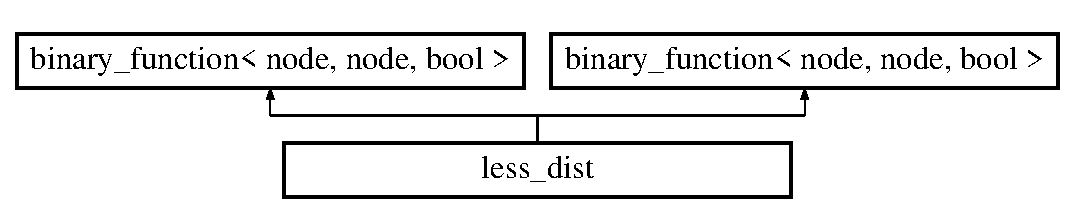
\includegraphics[height=2.000000cm]{classless__dist}
\end{center}
\end{figure}
\subsection*{Public Member Functions}
\begin{DoxyCompactItemize}
\item 
\mbox{\Hypertarget{classless__dist_a103396a9986a15a532b2e5eea09d5ac8}\label{classless__dist_a103396a9986a15a532b2e5eea09d5ac8}} 
{\bfseries less\+\_\+dist} (const \mbox{\hyperlink{classnode__map}{node\+\_\+map}}$<$ double $>$ $\ast$dist, const \mbox{\hyperlink{classnode__map}{node\+\_\+map}}$<$ int $>$ $\ast$mark)
\item 
\mbox{\Hypertarget{classless__dist_ad60cec2a03ca609f0f4af0818ee9caeb}\label{classless__dist_ad60cec2a03ca609f0f4af0818ee9caeb}} 
bool {\bfseries operator()} (const \mbox{\hyperlink{classnode}{node}} n1, const \mbox{\hyperlink{classnode}{node}} n2) const
\item 
\mbox{\Hypertarget{classless__dist_a103396a9986a15a532b2e5eea09d5ac8}\label{classless__dist_a103396a9986a15a532b2e5eea09d5ac8}} 
{\bfseries less\+\_\+dist} (const \mbox{\hyperlink{classnode__map}{node\+\_\+map}}$<$ double $>$ $\ast$dist, const \mbox{\hyperlink{classnode__map}{node\+\_\+map}}$<$ int $>$ $\ast$mark)
\item 
\mbox{\Hypertarget{classless__dist_ad60cec2a03ca609f0f4af0818ee9caeb}\label{classless__dist_ad60cec2a03ca609f0f4af0818ee9caeb}} 
bool {\bfseries operator()} (const \mbox{\hyperlink{classnode}{node}} n1, const \mbox{\hyperlink{classnode}{node}} n2) const
\end{DoxyCompactItemize}


The documentation for this class was generated from the following files\+:\begin{DoxyCompactItemize}
\item 
src/bid\+\_\+dijkstra.\+cpp\item 
src/dijkstra.\+cpp\end{DoxyCompactItemize}

\hypertarget{classmaxflow__ff}{}\section{maxflow\+\_\+ff Class Reference}
\label{classmaxflow__ff}\index{maxflow\+\_\+ff@{maxflow\+\_\+ff}}


Maximum flow algorithm (Edmonds-\/\+Karp).  




{\ttfamily \#include $<$maxflow\+\_\+ff.\+h$>$}

Inheritance diagram for maxflow\+\_\+ff\+:\begin{figure}[H]
\begin{center}
\leavevmode
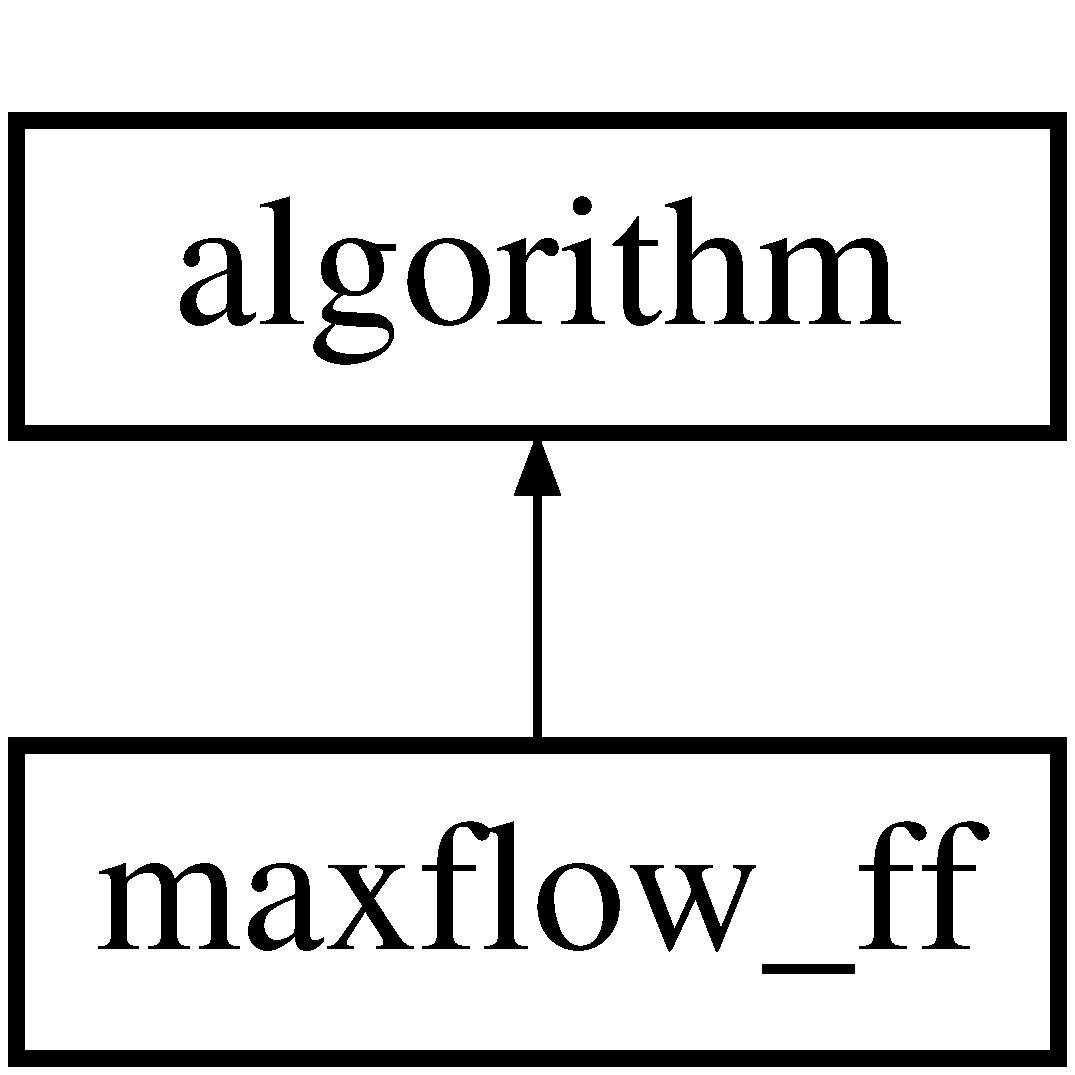
\includegraphics[height=2.000000cm]{classmaxflow__ff}
\end{center}
\end{figure}
\subsection*{Public Member Functions}
\begin{DoxyCompactItemize}
\item 
\mbox{\hyperlink{classmaxflow__ff_a47280ecd91e227e529455249ee390ca3}{maxflow\+\_\+ff}} ()
\item 
virtual \mbox{\hyperlink{classmaxflow__ff_ae1c3c5ba0b8c55cdba429ee906bce7d9}{$\sim$maxflow\+\_\+ff}} ()
\item 
void \mbox{\hyperlink{classmaxflow__ff_ad2485a4c093dbcfa045d1e6e5d78f533}{set\+\_\+vars}} (const \mbox{\hyperlink{classedge__map}{edge\+\_\+map}}$<$ double $>$ \&edge\+\_\+capacity)
\item 
void \mbox{\hyperlink{classmaxflow__ff_a1e715030d70080e0c9ecf118dd81e8f6}{set\+\_\+vars}} (const \mbox{\hyperlink{classedge__map}{edge\+\_\+map}}$<$ double $>$ \&edge\+\_\+capacity, const \mbox{\hyperlink{classnode}{node}} \&net\+\_\+source, const \mbox{\hyperlink{classnode}{node}} \&net\+\_\+target)
\item 
virtual int \mbox{\hyperlink{classmaxflow__ff_a4d0deee7d70bac4c9dad942341d87e37}{check}} (\mbox{\hyperlink{classgraph}{graph}} \&G)
\item 
int \mbox{\hyperlink{classmaxflow__ff_a0a4391b9093d6966b47c023a555099e2}{run}} (\mbox{\hyperlink{classgraph}{graph}} \&G)
\item 
double \mbox{\hyperlink{classmaxflow__ff_a4c120a7ea9be23d908036ebd2fb9298c}{get\+\_\+max\+\_\+flow}} (const \mbox{\hyperlink{classedge}{edge}} \&e) const
\item 
double \mbox{\hyperlink{classmaxflow__ff_a04d1ea509c13e500b62cad061ee8a2b9}{get\+\_\+max\+\_\+flow}} () const
\item 
double \mbox{\hyperlink{classmaxflow__ff_a3b66acf996ff5be94de8b2cfdb3164c3}{get\+\_\+rem\+\_\+cap}} (const \mbox{\hyperlink{classedge}{edge}} \&e) const
\item 
virtual void \mbox{\hyperlink{classmaxflow__ff_a893e5136d4f7f1d4b67ef5b67306d17b}{reset}} ()
\end{DoxyCompactItemize}
\subsection*{Protected Types}
\begin{DoxyCompactItemize}
\item 
\mbox{\Hypertarget{classmaxflow__ff_a08dc6e5c5fe20a9f9d93721f8c273592}\label{classmaxflow__ff_a08dc6e5c5fe20a9f9d93721f8c273592}} 
enum \{ {\bfseries S\+P\+\_\+\+F\+O\+U\+ND} = 2, 
{\bfseries N\+O\+\_\+\+S\+P\+\_\+\+F\+O\+U\+ND} = 3
 \}
\end{DoxyCompactItemize}
\subsection*{Protected Member Functions}
\begin{DoxyCompactItemize}
\item 
\mbox{\Hypertarget{classmaxflow__ff_ad2634e4325012773d793e9cf8f1a3dcf}\label{classmaxflow__ff_ad2634e4325012773d793e9cf8f1a3dcf}} 
void {\bfseries create\+\_\+artif\+\_\+source\+\_\+target} (\mbox{\hyperlink{classgraph}{graph}} \&G)
\item 
\mbox{\Hypertarget{classmaxflow__ff_a8ad20b45a7d30070bb65e68758c2f7d3}\label{classmaxflow__ff_a8ad20b45a7d30070bb65e68758c2f7d3}} 
void {\bfseries prepare\+\_\+run} (const \mbox{\hyperlink{classgraph}{graph}} \&G)
\item 
\mbox{\Hypertarget{classmaxflow__ff_a22a432bb072e0410f20bb418dfd4d3a9}\label{classmaxflow__ff_a22a432bb072e0410f20bb418dfd4d3a9}} 
void {\bfseries comp\+\_\+single\+\_\+flow} (\mbox{\hyperlink{classgraph}{graph}} \&G, \mbox{\hyperlink{classnode__map}{node\+\_\+map}}$<$ \mbox{\hyperlink{classedge}{edge}} $>$ \&last\+\_\+edge)
\item 
\mbox{\Hypertarget{classmaxflow__ff_a532b1285a791d23ab318791bc093fde7}\label{classmaxflow__ff_a532b1285a791d23ab318791bc093fde7}} 
int {\bfseries get\+\_\+sp} (const \mbox{\hyperlink{classgraph}{graph}} \&G, \mbox{\hyperlink{classnode__map}{node\+\_\+map}}$<$ \mbox{\hyperlink{classedge}{edge}} $>$ \&last\+\_\+edge)
\item 
\mbox{\Hypertarget{classmaxflow__ff_a3a9d93d6796ae0846d0137aa46f29c30}\label{classmaxflow__ff_a3a9d93d6796ae0846d0137aa46f29c30}} 
int {\bfseries comp\+\_\+sp} (const \mbox{\hyperlink{classgraph}{graph}} \&G, queue$<$ \mbox{\hyperlink{classnode}{node}} $>$ \&next\+\_\+nodes, \mbox{\hyperlink{classnode__map}{node\+\_\+map}}$<$ bool $>$ \&visited, \mbox{\hyperlink{classnode__map}{node\+\_\+map}}$<$ \mbox{\hyperlink{classedge}{edge}} $>$ \&last\+\_\+edge)
\item 
\mbox{\Hypertarget{classmaxflow__ff_a410a7c5b9b75225ec0a48402dc2f6555}\label{classmaxflow__ff_a410a7c5b9b75225ec0a48402dc2f6555}} 
double {\bfseries extra\+\_\+charge} (const \mbox{\hyperlink{classnode__map}{node\+\_\+map}}$<$ \mbox{\hyperlink{classedge}{edge}} $>$ \&last\+\_\+edge) const
\item 
\mbox{\Hypertarget{classmaxflow__ff_aea04831f46fb86990c9ba21fb19d0382}\label{classmaxflow__ff_aea04831f46fb86990c9ba21fb19d0382}} 
void {\bfseries create\+\_\+back\+\_\+edge} (\mbox{\hyperlink{classgraph}{graph}} \&G, const \mbox{\hyperlink{classedge}{edge}} \&org\+\_\+edge)
\item 
\mbox{\Hypertarget{classmaxflow__ff_a560d27c4c62b46dcb0a36ac60ebc1efb}\label{classmaxflow__ff_a560d27c4c62b46dcb0a36ac60ebc1efb}} 
void {\bfseries comp\+\_\+max\+\_\+flow} (const \mbox{\hyperlink{classgraph}{graph}} \&G)
\item 
\mbox{\Hypertarget{classmaxflow__ff_a31a13c79918964a49fa18b4eb514c584}\label{classmaxflow__ff_a31a13c79918964a49fa18b4eb514c584}} 
void {\bfseries restore\+\_\+graph} (\mbox{\hyperlink{classgraph}{graph}} \&G)
\end{DoxyCompactItemize}
\subsection*{Protected Attributes}
\begin{DoxyCompactItemize}
\item 
\mbox{\Hypertarget{classmaxflow__ff_a1ec31e7053722875a2e90659f79396a3}\label{classmaxflow__ff_a1ec31e7053722875a2e90659f79396a3}} 
bool {\bfseries artif\+\_\+source\+\_\+target}
\item 
\mbox{\Hypertarget{classmaxflow__ff_a2551a00303d9b81ccc6b3d1f575d7956}\label{classmaxflow__ff_a2551a00303d9b81ccc6b3d1f575d7956}} 
bool {\bfseries set\+\_\+vars\+\_\+executed}
\item 
\mbox{\Hypertarget{classmaxflow__ff_a7a2f530f9c95b6f37f4c349427a0f9bb}\label{classmaxflow__ff_a7a2f530f9c95b6f37f4c349427a0f9bb}} 
double {\bfseries max\+\_\+graph\+\_\+flow}
\item 
\mbox{\Hypertarget{classmaxflow__ff_a2e4cc02ce8c9d929f2896525c686d6c1}\label{classmaxflow__ff_a2e4cc02ce8c9d929f2896525c686d6c1}} 
\mbox{\hyperlink{classnode}{node}} {\bfseries net\+\_\+source}
\item 
\mbox{\Hypertarget{classmaxflow__ff_a94d5db73364cf5824ec3d3d530b57319}\label{classmaxflow__ff_a94d5db73364cf5824ec3d3d530b57319}} 
\mbox{\hyperlink{classnode}{node}} {\bfseries net\+\_\+target}
\item 
\mbox{\Hypertarget{classmaxflow__ff_a5798d469fb86dc7635a36dcf327a1906}\label{classmaxflow__ff_a5798d469fb86dc7635a36dcf327a1906}} 
list$<$ \mbox{\hyperlink{classedge}{edge}} $>$ {\bfseries edges\+\_\+not\+\_\+org}
\item 
\mbox{\Hypertarget{classmaxflow__ff_aa9fd46b8da1a67678b132a17e7a41c91}\label{classmaxflow__ff_aa9fd46b8da1a67678b132a17e7a41c91}} 
\mbox{\hyperlink{classedge__map}{edge\+\_\+map}}$<$ bool $>$ {\bfseries edge\+\_\+org}
\item 
\mbox{\Hypertarget{classmaxflow__ff_a686006593b17dfd3ad9a5e02b1ad9e92}\label{classmaxflow__ff_a686006593b17dfd3ad9a5e02b1ad9e92}} 
\mbox{\hyperlink{classedge__map}{edge\+\_\+map}}$<$ bool $>$ {\bfseries back\+\_\+edge\+\_\+exists}
\item 
\mbox{\Hypertarget{classmaxflow__ff_abceef8f9ee5acf7a992301de6d0c80de}\label{classmaxflow__ff_abceef8f9ee5acf7a992301de6d0c80de}} 
\mbox{\hyperlink{classedge__map}{edge\+\_\+map}}$<$ \mbox{\hyperlink{classedge}{edge}} $>$ {\bfseries back\+\_\+edge}
\item 
\mbox{\Hypertarget{classmaxflow__ff_a5b38943e093c77a57eb70f1a4190b8a6}\label{classmaxflow__ff_a5b38943e093c77a57eb70f1a4190b8a6}} 
\mbox{\hyperlink{classedge__map}{edge\+\_\+map}}$<$ double $>$ {\bfseries edge\+\_\+capacity}
\item 
\mbox{\Hypertarget{classmaxflow__ff_a669f36f1fae2dd0f6cfc0172e3ae0e8f}\label{classmaxflow__ff_a669f36f1fae2dd0f6cfc0172e3ae0e8f}} 
\mbox{\hyperlink{classedge__map}{edge\+\_\+map}}$<$ double $>$ {\bfseries edge\+\_\+max\+\_\+flow}
\end{DoxyCompactItemize}
\subsection*{Additional Inherited Members}


\subsection{Detailed Description}
Maximum flow algorithm (Edmonds-\/\+Karp). 

\subsection{Constructor \& Destructor Documentation}
\mbox{\Hypertarget{classmaxflow__ff_a47280ecd91e227e529455249ee390ca3}\label{classmaxflow__ff_a47280ecd91e227e529455249ee390ca3}} 
\index{maxflow\+\_\+ff@{maxflow\+\_\+ff}!maxflow\+\_\+ff@{maxflow\+\_\+ff}}
\index{maxflow\+\_\+ff@{maxflow\+\_\+ff}!maxflow\+\_\+ff@{maxflow\+\_\+ff}}
\subsubsection{\texorpdfstring{maxflow\+\_\+ff()}{maxflow\_ff()}}
{\footnotesize\ttfamily \+\_\+\+\_\+\+K\+G\+L\+\_\+\+B\+E\+G\+I\+N\+\_\+\+N\+A\+M\+E\+S\+P\+A\+CE maxflow\+\_\+ff\+::maxflow\+\_\+ff (\begin{DoxyParamCaption}{ }\end{DoxyParamCaption})}

Default constructor. Enables only the calculation of maximum flow.

\begin{DoxySeeAlso}{See also}
\mbox{\hyperlink{classalgorithm_ab79e1ddec2f2afdf4b36b10724db8b15}{algorithm\+::algorithm}} 
\end{DoxySeeAlso}
\mbox{\Hypertarget{classmaxflow__ff_ae1c3c5ba0b8c55cdba429ee906bce7d9}\label{classmaxflow__ff_ae1c3c5ba0b8c55cdba429ee906bce7d9}} 
\index{maxflow\+\_\+ff@{maxflow\+\_\+ff}!````~maxflow\+\_\+ff@{$\sim$maxflow\+\_\+ff}}
\index{````~maxflow\+\_\+ff@{$\sim$maxflow\+\_\+ff}!maxflow\+\_\+ff@{maxflow\+\_\+ff}}
\subsubsection{\texorpdfstring{$\sim$maxflow\+\_\+ff()}{~maxflow\_ff()}}
{\footnotesize\ttfamily maxflow\+\_\+ff\+::$\sim$maxflow\+\_\+ff (\begin{DoxyParamCaption}{ }\end{DoxyParamCaption})\hspace{0.3cm}{\ttfamily [virtual]}}

Destructor.

\begin{DoxySeeAlso}{See also}
\mbox{\hyperlink{classalgorithm_adca9b1e7fa3afd914519a9dbb44e9fd5}{algorithm\+::$\sim$algorithm}} 
\end{DoxySeeAlso}


\subsection{Member Function Documentation}
\mbox{\Hypertarget{classmaxflow__ff_a4d0deee7d70bac4c9dad942341d87e37}\label{classmaxflow__ff_a4d0deee7d70bac4c9dad942341d87e37}} 
\index{maxflow\+\_\+ff@{maxflow\+\_\+ff}!check@{check}}
\index{check@{check}!maxflow\+\_\+ff@{maxflow\+\_\+ff}}
\subsubsection{\texorpdfstring{check()}{check()}}
{\footnotesize\ttfamily int maxflow\+\_\+ff\+::check (\begin{DoxyParamCaption}\item[{\mbox{\hyperlink{classgraph}{graph}} \&}]{G }\end{DoxyParamCaption})\hspace{0.3cm}{\ttfamily [virtual]}}

Checks whether following preconditions are satisfied\+: 
\begin{DoxyItemize}
\item \mbox{\hyperlink{classmaxflow__ff_ad2485a4c093dbcfa045d1e6e5d78f533}{maxflow\+\_\+ff\+::set\+\_\+vars}} has been executed before. 
\item only edge\+\_\+capacities $>$= 0 are applied. 
\item {\ttfamily G} is directed. 
\item {\ttfamily G} is connected. 
\item {\ttfamily G} has at least one edge and two nodes. 
\item if not applied, start-\/nodes and end-\/nodes exists. 
\item if applied, start-\/node is not the same node as end-\/node. 
\end{DoxyItemize}


\begin{DoxyParams}{Parameters}
{\em G} & graph \\
\hline
\end{DoxyParams}
\begin{DoxyReturn}{Returns}
{\ttfamily \mbox{\hyperlink{classalgorithm_af1a0078e153aa99c24f9bdf0d97f6710aae4c1cd7fe8d8cf4b143241a6e7c31cf}{algorithm\+::\+K\+G\+L\+\_\+\+OK}}} on success {\ttfamily \mbox{\hyperlink{classalgorithm_af1a0078e153aa99c24f9bdf0d97f6710ae67bf27b2ef31f73e545a7f9f4a69556}{algorithm\+::\+K\+G\+L\+\_\+\+E\+R\+R\+OR}}} otherwise 
\end{DoxyReturn}
\begin{DoxySeeAlso}{See also}
\mbox{\hyperlink{classalgorithm_a76361fb03ad1cf643affc51821e43bed}{algorithm\+::check}} 
\end{DoxySeeAlso}


Implements \mbox{\hyperlink{classalgorithm_a76361fb03ad1cf643affc51821e43bed}{algorithm}}.

\mbox{\Hypertarget{classmaxflow__ff_a4c120a7ea9be23d908036ebd2fb9298c}\label{classmaxflow__ff_a4c120a7ea9be23d908036ebd2fb9298c}} 
\index{maxflow\+\_\+ff@{maxflow\+\_\+ff}!get\+\_\+max\+\_\+flow@{get\+\_\+max\+\_\+flow}}
\index{get\+\_\+max\+\_\+flow@{get\+\_\+max\+\_\+flow}!maxflow\+\_\+ff@{maxflow\+\_\+ff}}
\subsubsection{\texorpdfstring{get\+\_\+max\+\_\+flow()}{get\_max\_flow()}\hspace{0.1cm}{\footnotesize\ttfamily [1/2]}}
{\footnotesize\ttfamily double maxflow\+\_\+ff\+::get\+\_\+max\+\_\+flow (\begin{DoxyParamCaption}\item[{const \mbox{\hyperlink{classedge}{edge}} \&}]{e }\end{DoxyParamCaption}) const}

Returns the maximum flow of an edge.


\begin{DoxyParams}{Parameters}
{\em e} & edge of a graph G \\
\hline
\end{DoxyParams}
\begin{DoxyReturn}{Returns}
maximum flow value 
\end{DoxyReturn}
\mbox{\Hypertarget{classmaxflow__ff_a04d1ea509c13e500b62cad061ee8a2b9}\label{classmaxflow__ff_a04d1ea509c13e500b62cad061ee8a2b9}} 
\index{maxflow\+\_\+ff@{maxflow\+\_\+ff}!get\+\_\+max\+\_\+flow@{get\+\_\+max\+\_\+flow}}
\index{get\+\_\+max\+\_\+flow@{get\+\_\+max\+\_\+flow}!maxflow\+\_\+ff@{maxflow\+\_\+ff}}
\subsubsection{\texorpdfstring{get\+\_\+max\+\_\+flow()}{get\_max\_flow()}\hspace{0.1cm}{\footnotesize\ttfamily [2/2]}}
{\footnotesize\ttfamily double maxflow\+\_\+ff\+::get\+\_\+max\+\_\+flow (\begin{DoxyParamCaption}{ }\end{DoxyParamCaption}) const}

Returns the maximum flow of the whole graph G.

\begin{DoxyReturn}{Returns}
maximum flow value 
\end{DoxyReturn}
\mbox{\Hypertarget{classmaxflow__ff_a3b66acf996ff5be94de8b2cfdb3164c3}\label{classmaxflow__ff_a3b66acf996ff5be94de8b2cfdb3164c3}} 
\index{maxflow\+\_\+ff@{maxflow\+\_\+ff}!get\+\_\+rem\+\_\+cap@{get\+\_\+rem\+\_\+cap}}
\index{get\+\_\+rem\+\_\+cap@{get\+\_\+rem\+\_\+cap}!maxflow\+\_\+ff@{maxflow\+\_\+ff}}
\subsubsection{\texorpdfstring{get\+\_\+rem\+\_\+cap()}{get\_rem\_cap()}}
{\footnotesize\ttfamily double maxflow\+\_\+ff\+::get\+\_\+rem\+\_\+cap (\begin{DoxyParamCaption}\item[{const \mbox{\hyperlink{classedge}{edge}} \&}]{e }\end{DoxyParamCaption}) const}

Returns the remaining free capacity of an edge.


\begin{DoxyParams}{Parameters}
{\em e} & edge of a graph G \\
\hline
\end{DoxyParams}
\begin{DoxyReturn}{Returns}
remaining capacity 
\end{DoxyReturn}
\mbox{\Hypertarget{classmaxflow__ff_a893e5136d4f7f1d4b67ef5b67306d17b}\label{classmaxflow__ff_a893e5136d4f7f1d4b67ef5b67306d17b}} 
\index{maxflow\+\_\+ff@{maxflow\+\_\+ff}!reset@{reset}}
\index{reset@{reset}!maxflow\+\_\+ff@{maxflow\+\_\+ff}}
\subsubsection{\texorpdfstring{reset()}{reset()}}
{\footnotesize\ttfamily void maxflow\+\_\+ff\+::reset (\begin{DoxyParamCaption}{ }\end{DoxyParamCaption})\hspace{0.3cm}{\ttfamily [virtual]}}

Resets maximum flow algorithm, i.\+e. prepares the algorithm to be applied to another graph.

\begin{DoxySeeAlso}{See also}
\mbox{\hyperlink{classalgorithm_a21aba63d066ae7897de6ca7d8425c408}{algorithm\+::reset}} 
\end{DoxySeeAlso}


Implements \mbox{\hyperlink{classalgorithm_a21aba63d066ae7897de6ca7d8425c408}{algorithm}}.

\mbox{\Hypertarget{classmaxflow__ff_a0a4391b9093d6966b47c023a555099e2}\label{classmaxflow__ff_a0a4391b9093d6966b47c023a555099e2}} 
\index{maxflow\+\_\+ff@{maxflow\+\_\+ff}!run@{run}}
\index{run@{run}!maxflow\+\_\+ff@{maxflow\+\_\+ff}}
\subsubsection{\texorpdfstring{run()}{run()}}
{\footnotesize\ttfamily int maxflow\+\_\+ff\+::run (\begin{DoxyParamCaption}\item[{\mbox{\hyperlink{classgraph}{graph}} \&}]{G }\end{DoxyParamCaption})\hspace{0.3cm}{\ttfamily [virtual]}}

Computes maximum flow of graph {\ttfamily G}.


\begin{DoxyParams}{Parameters}
{\em G} & graph \\
\hline
\end{DoxyParams}
\begin{DoxyReturn}{Returns}
{\ttfamily \mbox{\hyperlink{classalgorithm_af1a0078e153aa99c24f9bdf0d97f6710aae4c1cd7fe8d8cf4b143241a6e7c31cf}{algorithm\+::\+K\+G\+L\+\_\+\+OK}}} on success {\ttfamily \mbox{\hyperlink{classalgorithm_af1a0078e153aa99c24f9bdf0d97f6710ae67bf27b2ef31f73e545a7f9f4a69556}{algorithm\+::\+K\+G\+L\+\_\+\+E\+R\+R\+OR}}} otherwise 
\end{DoxyReturn}
\begin{DoxySeeAlso}{See also}
\mbox{\hyperlink{classalgorithm_a734b189509a8d6b56b65f8ff772d43ca}{algorithm\+::run}} 
\end{DoxySeeAlso}


Implements \mbox{\hyperlink{classalgorithm_a734b189509a8d6b56b65f8ff772d43ca}{algorithm}}.

\mbox{\Hypertarget{classmaxflow__ff_ad2485a4c093dbcfa045d1e6e5d78f533}\label{classmaxflow__ff_ad2485a4c093dbcfa045d1e6e5d78f533}} 
\index{maxflow\+\_\+ff@{maxflow\+\_\+ff}!set\+\_\+vars@{set\+\_\+vars}}
\index{set\+\_\+vars@{set\+\_\+vars}!maxflow\+\_\+ff@{maxflow\+\_\+ff}}
\subsubsection{\texorpdfstring{set\+\_\+vars()}{set\_vars()}\hspace{0.1cm}{\footnotesize\ttfamily [1/2]}}
{\footnotesize\ttfamily void maxflow\+\_\+ff\+::set\+\_\+vars (\begin{DoxyParamCaption}\item[{const \mbox{\hyperlink{classedge__map}{edge\+\_\+map}}$<$ double $>$ \&}]{edge\+\_\+capacity }\end{DoxyParamCaption})}

Sets capacity of every edge for maximum flow calculation where artificial start-\/node and end\+\_\+node will be computed automatically.


\begin{DoxyParams}{Parameters}
{\em edge\+\_\+capacity} & capacity of every edge \\
\hline
\end{DoxyParams}
\mbox{\Hypertarget{classmaxflow__ff_a1e715030d70080e0c9ecf118dd81e8f6}\label{classmaxflow__ff_a1e715030d70080e0c9ecf118dd81e8f6}} 
\index{maxflow\+\_\+ff@{maxflow\+\_\+ff}!set\+\_\+vars@{set\+\_\+vars}}
\index{set\+\_\+vars@{set\+\_\+vars}!maxflow\+\_\+ff@{maxflow\+\_\+ff}}
\subsubsection{\texorpdfstring{set\+\_\+vars()}{set\_vars()}\hspace{0.1cm}{\footnotesize\ttfamily [2/2]}}
{\footnotesize\ttfamily void maxflow\+\_\+ff\+::set\+\_\+vars (\begin{DoxyParamCaption}\item[{const \mbox{\hyperlink{classedge__map}{edge\+\_\+map}}$<$ double $>$ \&}]{edge\+\_\+capacity,  }\item[{const \mbox{\hyperlink{classnode}{node}} \&}]{net\+\_\+source,  }\item[{const \mbox{\hyperlink{classnode}{node}} \&}]{net\+\_\+target }\end{DoxyParamCaption})}

Sets capacity of every edge for maximum flow calculation


\begin{DoxyParams}{Parameters}
{\em edge\+\_\+capacity} & capacity of every edge \\
\hline
{\em net\+\_\+source} & start-\/node \\
\hline
{\em net\+\_\+target} & end-\/node \\
\hline
\end{DoxyParams}


The documentation for this class was generated from the following files\+:\begin{DoxyCompactItemize}
\item 
include/\+K\+G\+L/maxflow\+\_\+ff.\+h\item 
src/maxflow\+\_\+ff.\+cpp\end{DoxyCompactItemize}

\hypertarget{classmaxflow__pp}{}\section{maxflow\+\_\+pp Class Reference}
\label{classmaxflow__pp}\index{maxflow\+\_\+pp@{maxflow\+\_\+pp}}


Maximum flow algorithm (Malhotra, Kumar, Maheshwari).  




{\ttfamily \#include $<$maxflow\+\_\+pp.\+h$>$}

Inheritance diagram for maxflow\+\_\+pp\+:\begin{figure}[H]
\begin{center}
\leavevmode
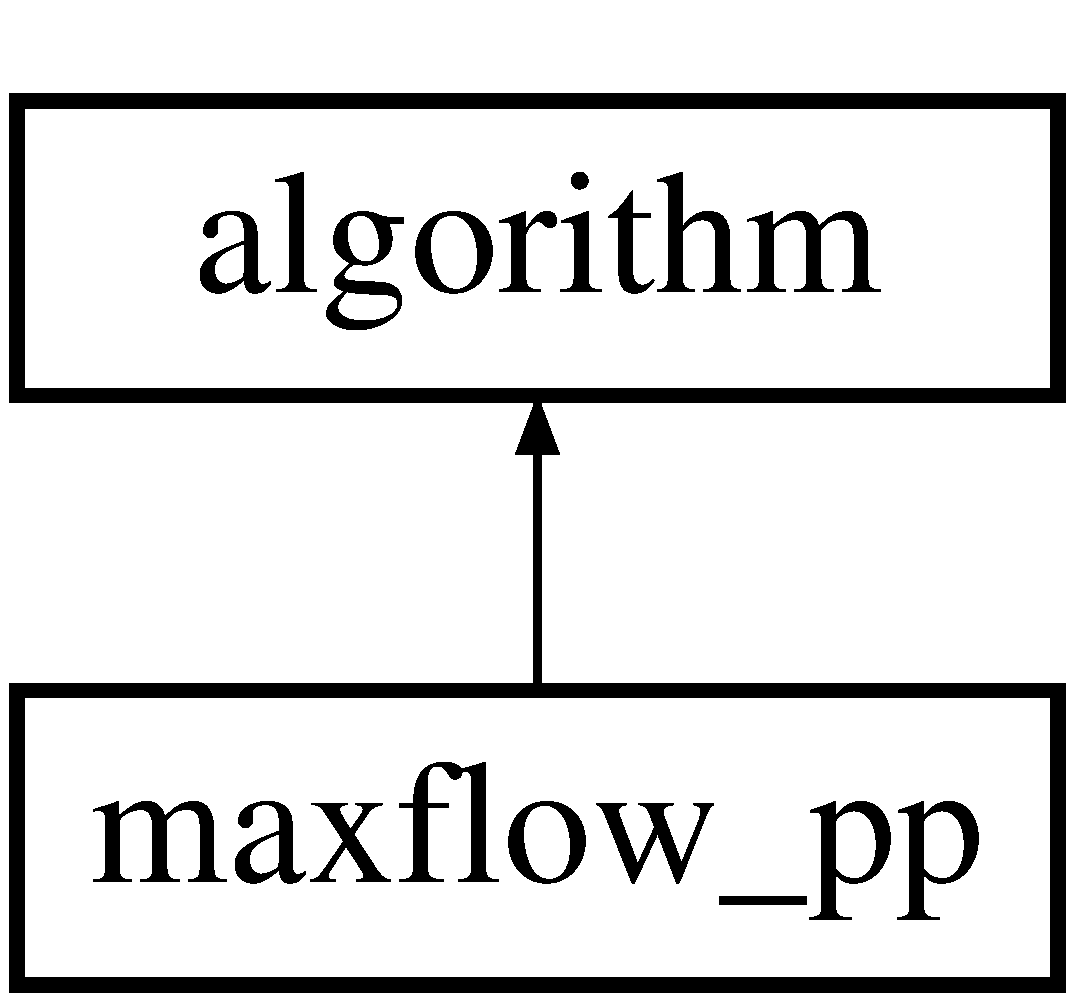
\includegraphics[height=2.000000cm]{classmaxflow__pp}
\end{center}
\end{figure}
\subsection*{Public Member Functions}
\begin{DoxyCompactItemize}
\item 
\mbox{\hyperlink{classmaxflow__pp_a29ec393f72f3289c49a79b0da17e3ccd}{maxflow\+\_\+pp}} ()
\item 
virtual \mbox{\hyperlink{classmaxflow__pp_a2f96bfeea4cb2c044d155d356d72452a}{$\sim$maxflow\+\_\+pp}} ()
\item 
void \mbox{\hyperlink{classmaxflow__pp_ac77f4c613efe7857e053f9bfb103dc3e}{set\+\_\+vars}} (const \mbox{\hyperlink{classedge__map}{edge\+\_\+map}}$<$ double $>$ \&edge\+\_\+capacity)
\item 
void \mbox{\hyperlink{classmaxflow__pp_a13756f76387cc114b88a44e324fc93ae}{set\+\_\+vars}} (const \mbox{\hyperlink{classedge__map}{edge\+\_\+map}}$<$ double $>$ \&edge\+\_\+capacity, const \mbox{\hyperlink{classnode}{node}} \&net\+\_\+source, const \mbox{\hyperlink{classnode}{node}} \&net\+\_\+target)
\item 
virtual auto \+\_\+\+\_\+cdecl \mbox{\hyperlink{classmaxflow__pp_a1535468f547b80ea750432f5e27c338d}{check}} (\mbox{\hyperlink{classgraph}{graph}} \&G) -\/$>$ int
\item 
auto \+\_\+\+\_\+cdecl \mbox{\hyperlink{classmaxflow__pp_a6c6fa792d7f0441048361778697e8e1e}{run}} (\mbox{\hyperlink{classgraph}{graph}} \&G) -\/$>$ int
\item 
double \mbox{\hyperlink{classmaxflow__pp_ac561a61619f363ef5d9b8fc5cfb10a5f}{get\+\_\+max\+\_\+flow}} (const \mbox{\hyperlink{classedge}{edge}} \&e) const
\item 
double \mbox{\hyperlink{classmaxflow__pp_a72210f8ac7aeca0a58e7407681003083}{get\+\_\+max\+\_\+flow}} () const
\item 
double \mbox{\hyperlink{classmaxflow__pp_ab3af0c0568ff2c8295166bfd75736169}{get\+\_\+rem\+\_\+cap}} (const \mbox{\hyperlink{classedge}{edge}} \&e) const
\item 
virtual auto \+\_\+\+\_\+cdecl \mbox{\hyperlink{classmaxflow__pp_a479e6e218f81d20acdc706b5771e38cb}{reset}} () -\/$>$ void
\end{DoxyCompactItemize}
\subsection*{Protected Types}
\begin{DoxyCompactItemize}
\item 
\mbox{\Hypertarget{classmaxflow__pp_abd042f1baa6a6200b5bbed755f400d2d}\label{classmaxflow__pp_abd042f1baa6a6200b5bbed755f400d2d}} 
enum \{ {\bfseries T\+A\+R\+G\+E\+T\+\_\+\+F\+R\+O\+M\+\_\+\+S\+O\+U\+R\+C\+E\+\_\+\+R\+E\+A\+C\+H\+A\+B\+LE} = 2, 
{\bfseries T\+A\+R\+G\+E\+T\+\_\+\+F\+R\+O\+M\+\_\+\+S\+O\+U\+R\+C\+E\+\_\+\+N\+O\+T\+\_\+\+R\+E\+A\+C\+H\+A\+B\+LE} = 3
 \}
\end{DoxyCompactItemize}
\subsection*{Protected Member Functions}
\begin{DoxyCompactItemize}
\item 
\mbox{\Hypertarget{classmaxflow__pp_a02438e89291eeccda0b247d20ffa11e5}\label{classmaxflow__pp_a02438e89291eeccda0b247d20ffa11e5}} 
void {\bfseries create\+\_\+artif\+\_\+source\+\_\+target} (\mbox{\hyperlink{classgraph}{graph}} \&G)
\item 
\mbox{\Hypertarget{classmaxflow__pp_a7a738741f8050df0cb0be0381aef0825}\label{classmaxflow__pp_a7a738741f8050df0cb0be0381aef0825}} 
void {\bfseries prepare\+\_\+run} (const \mbox{\hyperlink{classgraph}{graph}} \&G)
\item 
\mbox{\Hypertarget{classmaxflow__pp_adefb2cdc0145d57efd2d93c17a180896}\label{classmaxflow__pp_adefb2cdc0145d57efd2d93c17a180896}} 
int {\bfseries leveling} (\mbox{\hyperlink{classgraph}{graph}} \&G)
\item 
\mbox{\Hypertarget{classmaxflow__pp_a93bb037fd3fc83c6558b560fc4da2340}\label{classmaxflow__pp_a93bb037fd3fc83c6558b560fc4da2340}} 
void {\bfseries hide\+\_\+unreachable\+\_\+nodes} (\mbox{\hyperlink{classgraph}{graph}} \&G)
\item 
\mbox{\Hypertarget{classmaxflow__pp_abb23812a3e8bca1955b835d3c41836e1}\label{classmaxflow__pp_abb23812a3e8bca1955b835d3c41836e1}} 
void {\bfseries store\+\_\+temp\+\_\+unvisible\+\_\+edges} (const \mbox{\hyperlink{classnode}{node}} \&cur\+\_\+node)
\item 
\mbox{\Hypertarget{classmaxflow__pp_a9f820f51329f0e0ec4d8123547ae6ebd}\label{classmaxflow__pp_a9f820f51329f0e0ec4d8123547ae6ebd}} 
void {\bfseries min\+\_\+throughput\+\_\+node} (const \mbox{\hyperlink{classgraph}{graph}} \&G, \mbox{\hyperlink{classnode}{node}} \&min\+\_\+tp\+\_\+node, double \&min\+\_\+value)
\item 
\mbox{\Hypertarget{classmaxflow__pp_ab1146e40ae2f2405e0ca6ea3ff43a6ff}\label{classmaxflow__pp_ab1146e40ae2f2405e0ca6ea3ff43a6ff}} 
double {\bfseries comp\+\_\+min\+\_\+throughput} (const \mbox{\hyperlink{classnode}{node}} cur\+\_\+node) const
\item 
\mbox{\Hypertarget{classmaxflow__pp_a340e4b9909a44ed7003760017c761e3b}\label{classmaxflow__pp_a340e4b9909a44ed7003760017c761e3b}} 
void {\bfseries get\+\_\+sp\+\_\+ahead} (const \mbox{\hyperlink{classgraph}{graph}} \&G, const \mbox{\hyperlink{classnode}{node}} \&start\+\_\+node, \mbox{\hyperlink{classnode__map}{node\+\_\+map}}$<$ \mbox{\hyperlink{classedge}{edge}} $>$ \&last\+\_\+edge)
\item 
\mbox{\Hypertarget{classmaxflow__pp_a58b7af1b215766e99adcca0994ecfb7a}\label{classmaxflow__pp_a58b7af1b215766e99adcca0994ecfb7a}} 
void {\bfseries get\+\_\+sp\+\_\+backwards} (const \mbox{\hyperlink{classgraph}{graph}} \&G, const \mbox{\hyperlink{classnode}{node}} \&start\+\_\+node, \mbox{\hyperlink{classnode__map}{node\+\_\+map}}$<$ \mbox{\hyperlink{classedge}{edge}} $>$ \&prev\+\_\+edge)
\item 
\mbox{\Hypertarget{classmaxflow__pp_ae7c9ce8d1cad511d70022e2f62567590}\label{classmaxflow__pp_ae7c9ce8d1cad511d70022e2f62567590}} 
void {\bfseries push} (\mbox{\hyperlink{classgraph}{graph}} \&G, const \mbox{\hyperlink{classnode}{node}} \&start\+\_\+node, const double flow\+\_\+value)
\item 
\mbox{\Hypertarget{classmaxflow__pp_aba2aefadd6dde920b8b8aa44af95ad9b}\label{classmaxflow__pp_aba2aefadd6dde920b8b8aa44af95ad9b}} 
void {\bfseries pull} (\mbox{\hyperlink{classgraph}{graph}} \&G, const \mbox{\hyperlink{classnode}{node}} \&start\+\_\+node, const double flow\+\_\+value)
\item 
\mbox{\Hypertarget{classmaxflow__pp_a97612b9517f0f11715610cb8faa81606}\label{classmaxflow__pp_a97612b9517f0f11715610cb8faa81606}} 
void {\bfseries comp\+\_\+rem\+\_\+net} (\mbox{\hyperlink{classgraph}{graph}} \&G)
\item 
\mbox{\Hypertarget{classmaxflow__pp_a3e59652a416d1553f8a1d1229dd2cd38}\label{classmaxflow__pp_a3e59652a416d1553f8a1d1229dd2cd38}} 
void {\bfseries single\+\_\+edge\+\_\+update} (\mbox{\hyperlink{classgraph}{graph}} \&G, \mbox{\hyperlink{classedge}{edge}} cur\+\_\+edge)
\item 
\mbox{\Hypertarget{classmaxflow__pp_af60a96de8ef929ceefd32d387e8e1638}\label{classmaxflow__pp_af60a96de8ef929ceefd32d387e8e1638}} 
double {\bfseries extra\+\_\+charge\+\_\+ahead} (const \mbox{\hyperlink{classnode}{node}} \&start\+\_\+node, const \mbox{\hyperlink{classnode__map}{node\+\_\+map}}$<$ \mbox{\hyperlink{classedge}{edge}} $>$ \&last\+\_\+edge) const
\item 
\mbox{\Hypertarget{classmaxflow__pp_a9d9651e53139201506b22eed1ecbdd51}\label{classmaxflow__pp_a9d9651e53139201506b22eed1ecbdd51}} 
double {\bfseries extra\+\_\+charge\+\_\+backwards} (const \mbox{\hyperlink{classnode}{node}} \&start\+\_\+node, const \mbox{\hyperlink{classnode__map}{node\+\_\+map}}$<$ \mbox{\hyperlink{classedge}{edge}} $>$ \&prev\+\_\+edge) const
\item 
\mbox{\Hypertarget{classmaxflow__pp_a20abf72dadaac19acb027ff5fa62de2a}\label{classmaxflow__pp_a20abf72dadaac19acb027ff5fa62de2a}} 
void {\bfseries create\+\_\+back\+\_\+edge} (\mbox{\hyperlink{classgraph}{graph}} \&G, const \mbox{\hyperlink{classedge}{edge}} \&org\+\_\+edge)
\item 
\mbox{\Hypertarget{classmaxflow__pp_a6a8a301739757493318b1abfbed2698b}\label{classmaxflow__pp_a6a8a301739757493318b1abfbed2698b}} 
void {\bfseries comp\+\_\+max\+\_\+flow} (const \mbox{\hyperlink{classgraph}{graph}} \&G)
\item 
\mbox{\Hypertarget{classmaxflow__pp_a273cc9bde3aeb47c08223da7458ed29d}\label{classmaxflow__pp_a273cc9bde3aeb47c08223da7458ed29d}} 
void {\bfseries restore\+\_\+graph} (\mbox{\hyperlink{classgraph}{graph}} \&G)
\end{DoxyCompactItemize}
\subsection*{Protected Attributes}
\begin{DoxyCompactItemize}
\item 
\mbox{\Hypertarget{classmaxflow__pp_a21263af726420d377e404d816f31ed45}\label{classmaxflow__pp_a21263af726420d377e404d816f31ed45}} 
bool {\bfseries artif\+\_\+source\+\_\+target}
\item 
\mbox{\Hypertarget{classmaxflow__pp_a6642619150b9c12790df2171cfa2c05f}\label{classmaxflow__pp_a6642619150b9c12790df2171cfa2c05f}} 
bool {\bfseries set\+\_\+vars\+\_\+executed}
\item 
\mbox{\Hypertarget{classmaxflow__pp_abdda1871e70fd2de0f2006eff57dc94e}\label{classmaxflow__pp_abdda1871e70fd2de0f2006eff57dc94e}} 
double {\bfseries max\+\_\+graph\+\_\+flow}
\item 
\mbox{\Hypertarget{classmaxflow__pp_a20f2d05465acc2d7b777ea8025d12003}\label{classmaxflow__pp_a20f2d05465acc2d7b777ea8025d12003}} 
\mbox{\hyperlink{classnode}{node}} {\bfseries net\+\_\+source}
\item 
\mbox{\Hypertarget{classmaxflow__pp_a10f0b047011e04cb4816a824da5b7892}\label{classmaxflow__pp_a10f0b047011e04cb4816a824da5b7892}} 
\mbox{\hyperlink{classnode}{node}} {\bfseries net\+\_\+target}
\item 
\mbox{\Hypertarget{classmaxflow__pp_a15710242a1285c21811768ea85855004}\label{classmaxflow__pp_a15710242a1285c21811768ea85855004}} 
list$<$ \mbox{\hyperlink{classedge}{edge}} $>$ {\bfseries edges\+\_\+not\+\_\+org}
\item 
\mbox{\Hypertarget{classmaxflow__pp_aca9ce457300e11b97cec3446315fda1c}\label{classmaxflow__pp_aca9ce457300e11b97cec3446315fda1c}} 
\mbox{\hyperlink{classedge__map}{edge\+\_\+map}}$<$ bool $>$ {\bfseries edge\+\_\+org}
\item 
\mbox{\Hypertarget{classmaxflow__pp_a50e9c82f1e720b8340ea4dc6d438f110}\label{classmaxflow__pp_a50e9c82f1e720b8340ea4dc6d438f110}} 
\mbox{\hyperlink{classedge__map}{edge\+\_\+map}}$<$ bool $>$ {\bfseries back\+\_\+edge\+\_\+exists}
\item 
\mbox{\Hypertarget{classmaxflow__pp_a9fdef5a86459eaf9634737094f3de250}\label{classmaxflow__pp_a9fdef5a86459eaf9634737094f3de250}} 
\mbox{\hyperlink{classedge__map}{edge\+\_\+map}}$<$ \mbox{\hyperlink{classedge}{edge}} $>$ {\bfseries back\+\_\+edge}
\item 
\mbox{\Hypertarget{classmaxflow__pp_af3cdc4999a86322271a80b1855d58629}\label{classmaxflow__pp_af3cdc4999a86322271a80b1855d58629}} 
\mbox{\hyperlink{classedge__map}{edge\+\_\+map}}$<$ double $>$ {\bfseries edge\+\_\+capacity}
\item 
\mbox{\Hypertarget{classmaxflow__pp_a25d5bb2ab6c775a634dacf408ff55a83}\label{classmaxflow__pp_a25d5bb2ab6c775a634dacf408ff55a83}} 
\mbox{\hyperlink{classedge__map}{edge\+\_\+map}}$<$ double $>$ {\bfseries edge\+\_\+max\+\_\+flow}
\item 
\mbox{\Hypertarget{classmaxflow__pp_ad37aff831935b2cfd4b03bc4a6da06ce}\label{classmaxflow__pp_ad37aff831935b2cfd4b03bc4a6da06ce}} 
\mbox{\hyperlink{classedge__map}{edge\+\_\+map}}$<$ double $>$ {\bfseries flow\+\_\+update}
\item 
\mbox{\Hypertarget{classmaxflow__pp_a55e32031f4f54b5cc934bc0307feca42}\label{classmaxflow__pp_a55e32031f4f54b5cc934bc0307feca42}} 
list$<$ \mbox{\hyperlink{classedge}{edge}} $>$ {\bfseries full\+\_\+edges}
\item 
\mbox{\Hypertarget{classmaxflow__pp_adf78e195b91cca1948074d77d535a9a9}\label{classmaxflow__pp_adf78e195b91cca1948074d77d535a9a9}} 
list$<$ \mbox{\hyperlink{classnode}{node}} $>$ {\bfseries temp\+\_\+unvisible\+\_\+nodes}
\item 
\mbox{\Hypertarget{classmaxflow__pp_a5a0ede769352a2f29a261c4ce169cb02}\label{classmaxflow__pp_a5a0ede769352a2f29a261c4ce169cb02}} 
list$<$ \mbox{\hyperlink{classedge}{edge}} $>$ {\bfseries temp\+\_\+unvisible\+\_\+edges}
\end{DoxyCompactItemize}
\subsection*{Additional Inherited Members}


\subsection{Detailed Description}
Maximum flow algorithm (Malhotra, Kumar, Maheshwari). 

\subsection{Constructor \& Destructor Documentation}
\mbox{\Hypertarget{classmaxflow__pp_a29ec393f72f3289c49a79b0da17e3ccd}\label{classmaxflow__pp_a29ec393f72f3289c49a79b0da17e3ccd}} 
\index{maxflow\+\_\+pp@{maxflow\+\_\+pp}!maxflow\+\_\+pp@{maxflow\+\_\+pp}}
\index{maxflow\+\_\+pp@{maxflow\+\_\+pp}!maxflow\+\_\+pp@{maxflow\+\_\+pp}}
\subsubsection{\texorpdfstring{maxflow\+\_\+pp()}{maxflow\_pp()}}
{\footnotesize\ttfamily \+\_\+\+\_\+\+K\+G\+L\+\_\+\+B\+E\+G\+I\+N\+\_\+\+N\+A\+M\+E\+S\+P\+A\+CE maxflow\+\_\+pp\+::maxflow\+\_\+pp (\begin{DoxyParamCaption}{ }\end{DoxyParamCaption})}

Default constructor. Enables only the calculation of maximum flow.

\begin{DoxySeeAlso}{See also}
\mbox{\hyperlink{classalgorithm_ab79e1ddec2f2afdf4b36b10724db8b15}{algorithm\+::algorithm}} 
\end{DoxySeeAlso}
\mbox{\Hypertarget{classmaxflow__pp_a2f96bfeea4cb2c044d155d356d72452a}\label{classmaxflow__pp_a2f96bfeea4cb2c044d155d356d72452a}} 
\index{maxflow\+\_\+pp@{maxflow\+\_\+pp}!````~maxflow\+\_\+pp@{$\sim$maxflow\+\_\+pp}}
\index{````~maxflow\+\_\+pp@{$\sim$maxflow\+\_\+pp}!maxflow\+\_\+pp@{maxflow\+\_\+pp}}
\subsubsection{\texorpdfstring{$\sim$maxflow\+\_\+pp()}{~maxflow\_pp()}}
{\footnotesize\ttfamily maxflow\+\_\+pp\+::$\sim$maxflow\+\_\+pp (\begin{DoxyParamCaption}{ }\end{DoxyParamCaption})\hspace{0.3cm}{\ttfamily [virtual]}}

Destructor.

\begin{DoxySeeAlso}{See also}
\mbox{\hyperlink{classalgorithm_adca9b1e7fa3afd914519a9dbb44e9fd5}{algorithm\+::$\sim$algorithm}} 
\end{DoxySeeAlso}


\subsection{Member Function Documentation}
\mbox{\Hypertarget{classmaxflow__pp_a1535468f547b80ea750432f5e27c338d}\label{classmaxflow__pp_a1535468f547b80ea750432f5e27c338d}} 
\index{maxflow\+\_\+pp@{maxflow\+\_\+pp}!check@{check}}
\index{check@{check}!maxflow\+\_\+pp@{maxflow\+\_\+pp}}
\subsubsection{\texorpdfstring{check()}{check()}}
{\footnotesize\ttfamily int maxflow\+\_\+pp\+::check (\begin{DoxyParamCaption}\item[{\mbox{\hyperlink{classgraph}{graph}} \&}]{G }\end{DoxyParamCaption}) -\/$>$ int\hspace{0.3cm}{\ttfamily [virtual]}}

Checks whether following preconditions are satisfied\+: 
\begin{DoxyItemize}
\item \mbox{\hyperlink{classmaxflow__pp_ac77f4c613efe7857e053f9bfb103dc3e}{maxflow\+\_\+pp\+::set\+\_\+vars}} has been executed before. 
\item only edge\+\_\+capacities $>$= 0 are applied. 
\item {\ttfamily G} is directed. 
\item {\ttfamily G} is connected. 
\item {\ttfamily G} has at least one edge and two nodes. 
\item if not applied, start-\/nodes and end-\/nodes exists. 
\item if applied, start-\/node is not the same node as end-\/node. 
\end{DoxyItemize}


\begin{DoxyParams}{Parameters}
{\em G} & graph \\
\hline
\end{DoxyParams}
\begin{DoxyReturn}{Returns}
{\ttfamily \mbox{\hyperlink{classalgorithm_af1a0078e153aa99c24f9bdf0d97f6710aae4c1cd7fe8d8cf4b143241a6e7c31cf}{algorithm\+::\+K\+G\+L\+\_\+\+OK}}} on success {\ttfamily \mbox{\hyperlink{classalgorithm_af1a0078e153aa99c24f9bdf0d97f6710ae67bf27b2ef31f73e545a7f9f4a69556}{algorithm\+::\+K\+G\+L\+\_\+\+E\+R\+R\+OR}}} otherwise 
\end{DoxyReturn}
\begin{DoxySeeAlso}{See also}
\mbox{\hyperlink{classalgorithm_a05c0f25463eb35a77b2d73fc06bb2c0e}{algorithm\+::check}} 
\end{DoxySeeAlso}


Implements \mbox{\hyperlink{classalgorithm_a05c0f25463eb35a77b2d73fc06bb2c0e}{algorithm}}.

\mbox{\Hypertarget{classmaxflow__pp_ac561a61619f363ef5d9b8fc5cfb10a5f}\label{classmaxflow__pp_ac561a61619f363ef5d9b8fc5cfb10a5f}} 
\index{maxflow\+\_\+pp@{maxflow\+\_\+pp}!get\+\_\+max\+\_\+flow@{get\+\_\+max\+\_\+flow}}
\index{get\+\_\+max\+\_\+flow@{get\+\_\+max\+\_\+flow}!maxflow\+\_\+pp@{maxflow\+\_\+pp}}
\subsubsection{\texorpdfstring{get\+\_\+max\+\_\+flow()}{get\_max\_flow()}\hspace{0.1cm}{\footnotesize\ttfamily [1/2]}}
{\footnotesize\ttfamily double maxflow\+\_\+pp\+::get\+\_\+max\+\_\+flow (\begin{DoxyParamCaption}\item[{const \mbox{\hyperlink{classedge}{edge}} \&}]{e }\end{DoxyParamCaption}) const}

Returns the maximum flow of an edge.


\begin{DoxyParams}{Parameters}
{\em e} & edge of a graph {\ttfamily G} \\
\hline
\end{DoxyParams}
\begin{DoxyReturn}{Returns}
maximum flow value 
\end{DoxyReturn}
\mbox{\Hypertarget{classmaxflow__pp_a72210f8ac7aeca0a58e7407681003083}\label{classmaxflow__pp_a72210f8ac7aeca0a58e7407681003083}} 
\index{maxflow\+\_\+pp@{maxflow\+\_\+pp}!get\+\_\+max\+\_\+flow@{get\+\_\+max\+\_\+flow}}
\index{get\+\_\+max\+\_\+flow@{get\+\_\+max\+\_\+flow}!maxflow\+\_\+pp@{maxflow\+\_\+pp}}
\subsubsection{\texorpdfstring{get\+\_\+max\+\_\+flow()}{get\_max\_flow()}\hspace{0.1cm}{\footnotesize\ttfamily [2/2]}}
{\footnotesize\ttfamily double maxflow\+\_\+pp\+::get\+\_\+max\+\_\+flow (\begin{DoxyParamCaption}{ }\end{DoxyParamCaption}) const}

Returns the maximum flow of the whole graph {\ttfamily G}.

\begin{DoxyReturn}{Returns}
maximum flow value 
\end{DoxyReturn}
\mbox{\Hypertarget{classmaxflow__pp_ab3af0c0568ff2c8295166bfd75736169}\label{classmaxflow__pp_ab3af0c0568ff2c8295166bfd75736169}} 
\index{maxflow\+\_\+pp@{maxflow\+\_\+pp}!get\+\_\+rem\+\_\+cap@{get\+\_\+rem\+\_\+cap}}
\index{get\+\_\+rem\+\_\+cap@{get\+\_\+rem\+\_\+cap}!maxflow\+\_\+pp@{maxflow\+\_\+pp}}
\subsubsection{\texorpdfstring{get\+\_\+rem\+\_\+cap()}{get\_rem\_cap()}}
{\footnotesize\ttfamily double maxflow\+\_\+pp\+::get\+\_\+rem\+\_\+cap (\begin{DoxyParamCaption}\item[{const \mbox{\hyperlink{classedge}{edge}} \&}]{e }\end{DoxyParamCaption}) const}

Returns the remaining free capacity of an edge.


\begin{DoxyParams}{Parameters}
{\em e} & edge of a graph G \\
\hline
\end{DoxyParams}
\begin{DoxyReturn}{Returns}
remaining capacity 
\end{DoxyReturn}
\mbox{\Hypertarget{classmaxflow__pp_a479e6e218f81d20acdc706b5771e38cb}\label{classmaxflow__pp_a479e6e218f81d20acdc706b5771e38cb}} 
\index{maxflow\+\_\+pp@{maxflow\+\_\+pp}!reset@{reset}}
\index{reset@{reset}!maxflow\+\_\+pp@{maxflow\+\_\+pp}}
\subsubsection{\texorpdfstring{reset()}{reset()}}
{\footnotesize\ttfamily void maxflow\+\_\+pp\+::reset (\begin{DoxyParamCaption}{ }\end{DoxyParamCaption}) -\/$>$ void\hspace{0.3cm}{\ttfamily [virtual]}}

Resets maximum flow algorithm, i.\+e. prepares the algorithm to be applied to another graph. \begin{DoxySeeAlso}{See also}
\mbox{\hyperlink{classalgorithm_aea645f2e39976a477c8f8564656fd1b6}{algorithm\+::reset}} 
\end{DoxySeeAlso}


Implements \mbox{\hyperlink{classalgorithm_aea645f2e39976a477c8f8564656fd1b6}{algorithm}}.

\mbox{\Hypertarget{classmaxflow__pp_a6c6fa792d7f0441048361778697e8e1e}\label{classmaxflow__pp_a6c6fa792d7f0441048361778697e8e1e}} 
\index{maxflow\+\_\+pp@{maxflow\+\_\+pp}!run@{run}}
\index{run@{run}!maxflow\+\_\+pp@{maxflow\+\_\+pp}}
\subsubsection{\texorpdfstring{run()}{run()}}
{\footnotesize\ttfamily int maxflow\+\_\+pp\+::run (\begin{DoxyParamCaption}\item[{\mbox{\hyperlink{classgraph}{graph}} \&}]{G }\end{DoxyParamCaption}) -\/$>$ int\hspace{0.3cm}{\ttfamily [virtual]}}

Computes maximum flow of graph {\ttfamily G}.


\begin{DoxyParams}{Parameters}
{\em G} & graph \\
\hline
\end{DoxyParams}
\begin{DoxyReturn}{Returns}
{\ttfamily \mbox{\hyperlink{classalgorithm_af1a0078e153aa99c24f9bdf0d97f6710aae4c1cd7fe8d8cf4b143241a6e7c31cf}{algorithm\+::\+K\+G\+L\+\_\+\+OK}}} on success {\ttfamily \mbox{\hyperlink{classalgorithm_af1a0078e153aa99c24f9bdf0d97f6710ae67bf27b2ef31f73e545a7f9f4a69556}{algorithm\+::\+K\+G\+L\+\_\+\+E\+R\+R\+OR}}} otherwise 
\end{DoxyReturn}
\begin{DoxySeeAlso}{See also}
\mbox{\hyperlink{classalgorithm_a482eb28cacba018b5a86d3a819a50a2f}{algorithm\+::run}} 
\end{DoxySeeAlso}


Implements \mbox{\hyperlink{classalgorithm_a482eb28cacba018b5a86d3a819a50a2f}{algorithm}}.

\mbox{\Hypertarget{classmaxflow__pp_ac77f4c613efe7857e053f9bfb103dc3e}\label{classmaxflow__pp_ac77f4c613efe7857e053f9bfb103dc3e}} 
\index{maxflow\+\_\+pp@{maxflow\+\_\+pp}!set\+\_\+vars@{set\+\_\+vars}}
\index{set\+\_\+vars@{set\+\_\+vars}!maxflow\+\_\+pp@{maxflow\+\_\+pp}}
\subsubsection{\texorpdfstring{set\+\_\+vars()}{set\_vars()}\hspace{0.1cm}{\footnotesize\ttfamily [1/2]}}
{\footnotesize\ttfamily void maxflow\+\_\+pp\+::set\+\_\+vars (\begin{DoxyParamCaption}\item[{const \mbox{\hyperlink{classedge__map}{edge\+\_\+map}}$<$ double $>$ \&}]{edge\+\_\+capacity }\end{DoxyParamCaption})}

Sets capacity of every edge for maximum flow calculation where artificial start-\/node and end\+\_\+node will be computed automatically.


\begin{DoxyParams}{Parameters}
{\em edge\+\_\+capacity} & capacity of every edge \\
\hline
\end{DoxyParams}
\mbox{\Hypertarget{classmaxflow__pp_a13756f76387cc114b88a44e324fc93ae}\label{classmaxflow__pp_a13756f76387cc114b88a44e324fc93ae}} 
\index{maxflow\+\_\+pp@{maxflow\+\_\+pp}!set\+\_\+vars@{set\+\_\+vars}}
\index{set\+\_\+vars@{set\+\_\+vars}!maxflow\+\_\+pp@{maxflow\+\_\+pp}}
\subsubsection{\texorpdfstring{set\+\_\+vars()}{set\_vars()}\hspace{0.1cm}{\footnotesize\ttfamily [2/2]}}
{\footnotesize\ttfamily void maxflow\+\_\+pp\+::set\+\_\+vars (\begin{DoxyParamCaption}\item[{const \mbox{\hyperlink{classedge__map}{edge\+\_\+map}}$<$ double $>$ \&}]{edge\+\_\+capacity,  }\item[{const \mbox{\hyperlink{classnode}{node}} \&}]{net\+\_\+source,  }\item[{const \mbox{\hyperlink{classnode}{node}} \&}]{net\+\_\+target }\end{DoxyParamCaption})}

Sets capacity of every edge for maximum flow calculation


\begin{DoxyParams}{Parameters}
{\em edge\+\_\+capacity} & capacity of every edge \\
\hline
{\em net\+\_\+source} & start-\/node \\
\hline
{\em net\+\_\+target} & end-\/node \\
\hline
\end{DoxyParams}


The documentation for this class was generated from the following files\+:\begin{DoxyCompactItemize}
\item 
include/\+K\+G\+L/maxflow\+\_\+pp.\+h\item 
src/maxflow\+\_\+pp.\+cpp\end{DoxyCompactItemize}

\hypertarget{classmaxflow__sap}{}\section{maxflow\+\_\+sap Class Reference}
\label{classmaxflow__sap}\index{maxflow\+\_\+sap@{maxflow\+\_\+sap}}


Maximum flow algorithm with shortest augmenting paths.  




{\ttfamily \#include $<$maxflow\+\_\+sap.\+h$>$}

Inheritance diagram for maxflow\+\_\+sap\+:\begin{figure}[H]
\begin{center}
\leavevmode
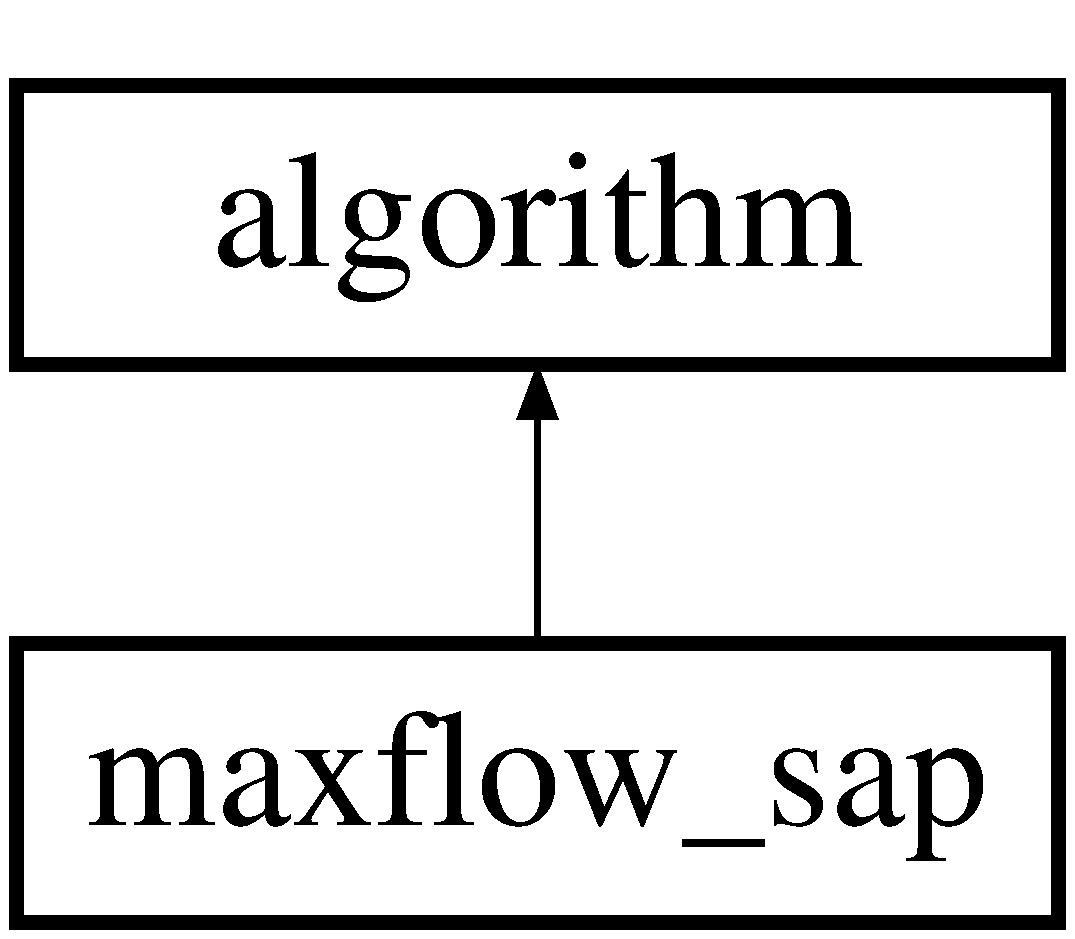
\includegraphics[height=2.000000cm]{classmaxflow__sap}
\end{center}
\end{figure}
\subsection*{Public Member Functions}
\begin{DoxyCompactItemize}
\item 
\mbox{\hyperlink{classmaxflow__sap_affc6e05aaa6d1b1455c99d6b5595a838}{maxflow\+\_\+sap}} ()
\item 
virtual \mbox{\hyperlink{classmaxflow__sap_ab49914afde43ffa0e5c3049cc063a8d2}{$\sim$maxflow\+\_\+sap}} ()
\item 
void \mbox{\hyperlink{classmaxflow__sap_ac50ba0330c169c7ce697947a76702e13}{set\+\_\+vars}} (const \mbox{\hyperlink{classedge__map}{edge\+\_\+map}}$<$ double $>$ \&edge\+\_\+capacity)
\item 
void \mbox{\hyperlink{classmaxflow__sap_a936f6afa25de80046c7bd69dc47fdfa9}{set\+\_\+vars}} (const \mbox{\hyperlink{classedge__map}{edge\+\_\+map}}$<$ double $>$ \&edge\+\_\+capacity, const \mbox{\hyperlink{classnode}{node}} \&net\+\_\+source, const \mbox{\hyperlink{classnode}{node}} \&net\+\_\+target)
\item 
virtual int \mbox{\hyperlink{classmaxflow__sap_aa2974bf25fb597677848fdb23c12d338}{check}} (\mbox{\hyperlink{classgraph}{graph}} \&G)
\item 
int \mbox{\hyperlink{classmaxflow__sap_ab4305a2bb370ad9c43cc68d339b2dda0}{run}} (\mbox{\hyperlink{classgraph}{graph}} \&G)
\item 
double \mbox{\hyperlink{classmaxflow__sap_ae90889b16323a2af0ab13e04c87953a5}{get\+\_\+max\+\_\+flow}} (const \mbox{\hyperlink{classedge}{edge}} \&e) const
\item 
double \mbox{\hyperlink{classmaxflow__sap_a81251d546cbdabc837f24fc3caf9fe0d}{get\+\_\+max\+\_\+flow}} () const
\item 
double \mbox{\hyperlink{classmaxflow__sap_a634835664542d5d181e1b63b99dda36c}{get\+\_\+rem\+\_\+cap}} (const \mbox{\hyperlink{classedge}{edge}} \&e) const
\item 
virtual void \mbox{\hyperlink{classmaxflow__sap_a14574d2f9ce31a3cdeb0888e57fc0616}{reset}} ()
\end{DoxyCompactItemize}
\subsection*{Protected Types}
\begin{DoxyCompactItemize}
\item 
\mbox{\Hypertarget{classmaxflow__sap_ac30ce6f46eb2dc97b557297c48989f8e}\label{classmaxflow__sap_ac30ce6f46eb2dc97b557297c48989f8e}} 
enum \{ {\bfseries A\+P\+\_\+\+F\+O\+U\+ND} = 2, 
{\bfseries N\+O\+\_\+\+A\+P\+\_\+\+F\+O\+U\+ND} = 3
 \}
\end{DoxyCompactItemize}
\subsection*{Protected Member Functions}
\begin{DoxyCompactItemize}
\item 
\mbox{\Hypertarget{classmaxflow__sap_a617016b94a4924fb2574ab87c970d49c}\label{classmaxflow__sap_a617016b94a4924fb2574ab87c970d49c}} 
void {\bfseries create\+\_\+artif\+\_\+source\+\_\+target} (\mbox{\hyperlink{classgraph}{graph}} \&G)
\item 
\mbox{\Hypertarget{classmaxflow__sap_a4504b071456d536371ff6d07055e800d}\label{classmaxflow__sap_a4504b071456d536371ff6d07055e800d}} 
void {\bfseries prepare\+\_\+run} (const \mbox{\hyperlink{classgraph}{graph}} \&G)
\item 
\mbox{\Hypertarget{classmaxflow__sap_a25424721feb100bdc357e2dfaff0f62c}\label{classmaxflow__sap_a25424721feb100bdc357e2dfaff0f62c}} 
void {\bfseries comp\+\_\+dist\+\_\+labels} (const \mbox{\hyperlink{classgraph}{graph}} \&G, vector$<$ int $>$ \&numb)
\item 
\mbox{\Hypertarget{classmaxflow__sap_a4fdfe2e37832ed2e522b5c972aa1ba5f}\label{classmaxflow__sap_a4fdfe2e37832ed2e522b5c972aa1ba5f}} 
bool {\bfseries has\+\_\+an\+\_\+admissible\+\_\+arc} (const \mbox{\hyperlink{classnode}{node}} cur\+\_\+node)
\item 
\mbox{\Hypertarget{classmaxflow__sap_a0eb02b00fa0840cfad87eb6d67c9b849}\label{classmaxflow__sap_a0eb02b00fa0840cfad87eb6d67c9b849}} 
void {\bfseries advance} (\mbox{\hyperlink{classnode}{node}} \&cur\+\_\+node, \mbox{\hyperlink{classnode__map}{node\+\_\+map}}$<$ \mbox{\hyperlink{classedge}{edge}} $>$ \&last\+\_\+edge)
\item 
\mbox{\Hypertarget{classmaxflow__sap_a02f7814313a36b30bb99c40ead6c9ef5}\label{classmaxflow__sap_a02f7814313a36b30bb99c40ead6c9ef5}} 
void {\bfseries augment} (\mbox{\hyperlink{classgraph}{graph}} \&G, const \mbox{\hyperlink{classnode__map}{node\+\_\+map}}$<$ \mbox{\hyperlink{classedge}{edge}} $>$ \&last\+\_\+edge)
\item 
\mbox{\Hypertarget{classmaxflow__sap_a72dc84d0f622655189cb586beb14b02b}\label{classmaxflow__sap_a72dc84d0f622655189cb586beb14b02b}} 
bool {\bfseries retreat} (const int number\+\_\+of\+\_\+nodes, \mbox{\hyperlink{classnode}{node}} \&cur\+\_\+node, const \mbox{\hyperlink{classnode__map}{node\+\_\+map}}$<$ \mbox{\hyperlink{classedge}{edge}} $>$ \&last\+\_\+edge, vector$<$ int $>$ \&numb)
\item 
\mbox{\Hypertarget{classmaxflow__sap_a7cf86463129a569f41883fdad6869fce}\label{classmaxflow__sap_a7cf86463129a569f41883fdad6869fce}} 
int {\bfseries min\+\_\+neighbour\+\_\+label} (const int number\+\_\+of\+\_\+nodes, const \mbox{\hyperlink{classnode}{node}} cur\+\_\+node) const
\item 
\mbox{\Hypertarget{classmaxflow__sap_abd2935db387f32891228291a52d6ad45}\label{classmaxflow__sap_abd2935db387f32891228291a52d6ad45}} 
double {\bfseries free\+\_\+capacity} (const \mbox{\hyperlink{classnode__map}{node\+\_\+map}}$<$ \mbox{\hyperlink{classedge}{edge}} $>$ \&last\+\_\+edge) const
\item 
\mbox{\Hypertarget{classmaxflow__sap_a4278d120bdbc505abb176f5ca6ba02b3}\label{classmaxflow__sap_a4278d120bdbc505abb176f5ca6ba02b3}} 
void {\bfseries create\+\_\+back\+\_\+edge} (\mbox{\hyperlink{classgraph}{graph}} \&G, const \mbox{\hyperlink{classedge}{edge}} \&org\+\_\+edge)
\item 
\mbox{\Hypertarget{classmaxflow__sap_ae5ff08e7b1c5fe5845a2ed584b04ca1b}\label{classmaxflow__sap_ae5ff08e7b1c5fe5845a2ed584b04ca1b}} 
void {\bfseries comp\+\_\+max\+\_\+flow} (const \mbox{\hyperlink{classgraph}{graph}} \&G)
\item 
\mbox{\Hypertarget{classmaxflow__sap_ad1a311df47e4b9936ead7c306d723ed0}\label{classmaxflow__sap_ad1a311df47e4b9936ead7c306d723ed0}} 
void {\bfseries restore\+\_\+graph} (\mbox{\hyperlink{classgraph}{graph}} \&G)
\end{DoxyCompactItemize}
\subsection*{Protected Attributes}
\begin{DoxyCompactItemize}
\item 
\mbox{\Hypertarget{classmaxflow__sap_a5d19d178a861e252c84fc392e19bf0ae}\label{classmaxflow__sap_a5d19d178a861e252c84fc392e19bf0ae}} 
bool {\bfseries artif\+\_\+source\+\_\+target}
\item 
\mbox{\Hypertarget{classmaxflow__sap_aad7f764b9e9732b996f402ffadbf5b70}\label{classmaxflow__sap_aad7f764b9e9732b996f402ffadbf5b70}} 
bool {\bfseries set\+\_\+vars\+\_\+executed}
\item 
\mbox{\Hypertarget{classmaxflow__sap_a77c650fd11632352a1228f2cbd38caf1}\label{classmaxflow__sap_a77c650fd11632352a1228f2cbd38caf1}} 
double {\bfseries max\+\_\+graph\+\_\+flow}
\item 
\mbox{\Hypertarget{classmaxflow__sap_abd4266c76dbd73f7f719d3a4fba2655d}\label{classmaxflow__sap_abd4266c76dbd73f7f719d3a4fba2655d}} 
\mbox{\hyperlink{classnode}{node}} {\bfseries net\+\_\+source}
\item 
\mbox{\Hypertarget{classmaxflow__sap_a8d0e8f448ed29a1329a70c8f4f496c2c}\label{classmaxflow__sap_a8d0e8f448ed29a1329a70c8f4f496c2c}} 
\mbox{\hyperlink{classnode}{node}} {\bfseries net\+\_\+target}
\item 
\mbox{\Hypertarget{classmaxflow__sap_a70cd2190558b44af3a4300256317dca5}\label{classmaxflow__sap_a70cd2190558b44af3a4300256317dca5}} 
list$<$ \mbox{\hyperlink{classedge}{edge}} $>$ {\bfseries edges\+\_\+not\+\_\+org}
\item 
\mbox{\Hypertarget{classmaxflow__sap_a14eef09823ae0ac69348c2b3a60e6ca3}\label{classmaxflow__sap_a14eef09823ae0ac69348c2b3a60e6ca3}} 
\mbox{\hyperlink{classnode__map}{node\+\_\+map}}$<$ int $>$ {\bfseries dist\+\_\+label}
\item 
\mbox{\Hypertarget{classmaxflow__sap_ac445d8c2f7e2080e890a9cdf7413c372}\label{classmaxflow__sap_ac445d8c2f7e2080e890a9cdf7413c372}} 
\mbox{\hyperlink{classedge__map}{edge\+\_\+map}}$<$ bool $>$ {\bfseries edge\+\_\+org}
\item 
\mbox{\Hypertarget{classmaxflow__sap_a13f2b98efc2a4f62fab4ac391ca83a51}\label{classmaxflow__sap_a13f2b98efc2a4f62fab4ac391ca83a51}} 
\mbox{\hyperlink{classedge__map}{edge\+\_\+map}}$<$ bool $>$ {\bfseries back\+\_\+edge\+\_\+exists}
\item 
\mbox{\Hypertarget{classmaxflow__sap_a34793d0909089155a9957deed7c0e1b7}\label{classmaxflow__sap_a34793d0909089155a9957deed7c0e1b7}} 
\mbox{\hyperlink{classedge__map}{edge\+\_\+map}}$<$ \mbox{\hyperlink{classedge}{edge}} $>$ {\bfseries back\+\_\+edge}
\item 
\mbox{\Hypertarget{classmaxflow__sap_acfa95eef5ea5bf7814c4dabd3994bc63}\label{classmaxflow__sap_acfa95eef5ea5bf7814c4dabd3994bc63}} 
\mbox{\hyperlink{classedge__map}{edge\+\_\+map}}$<$ double $>$ {\bfseries edge\+\_\+capacity}
\item 
\mbox{\Hypertarget{classmaxflow__sap_a25820db833a98efc69fc3edb79fc49d3}\label{classmaxflow__sap_a25820db833a98efc69fc3edb79fc49d3}} 
\mbox{\hyperlink{classedge__map}{edge\+\_\+map}}$<$ double $>$ {\bfseries edge\+\_\+max\+\_\+flow}
\end{DoxyCompactItemize}
\subsection*{Additional Inherited Members}


\subsection{Detailed Description}
Maximum flow algorithm with shortest augmenting paths. 

This class implements a maximum flow algorithm with shortest augmenting paths due to Ahuja and Orlin.

In the case V is the set of vertices and E is the set of edges of the graph, the algorithm needs O($\vert$\+V$\vert$ $\ast$ $\vert$\+V$\vert$ $\ast$ $\vert$\+E$\vert$) time to proceed.

\begin{DoxySeeAlso}{See also}
\mbox{\hyperlink{classmaxflow__ff}{maxflow\+\_\+ff}} 

\mbox{\hyperlink{classmaxflow__pp}{maxflow\+\_\+pp}} 
\end{DoxySeeAlso}


\subsection{Constructor \& Destructor Documentation}
\mbox{\Hypertarget{classmaxflow__sap_affc6e05aaa6d1b1455c99d6b5595a838}\label{classmaxflow__sap_affc6e05aaa6d1b1455c99d6b5595a838}} 
\index{maxflow\+\_\+sap@{maxflow\+\_\+sap}!maxflow\+\_\+sap@{maxflow\+\_\+sap}}
\index{maxflow\+\_\+sap@{maxflow\+\_\+sap}!maxflow\+\_\+sap@{maxflow\+\_\+sap}}
\subsubsection{\texorpdfstring{maxflow\+\_\+sap()}{maxflow\_sap()}}
{\footnotesize\ttfamily \+\_\+\+\_\+\+K\+G\+L\+\_\+\+B\+E\+G\+I\+N\+\_\+\+N\+A\+M\+E\+S\+P\+A\+CE maxflow\+\_\+sap\+::maxflow\+\_\+sap (\begin{DoxyParamCaption}{ }\end{DoxyParamCaption})}

Default constructor. Enables only the calculation of maximum flow.

\begin{DoxySeeAlso}{See also}
\mbox{\hyperlink{classalgorithm_ab79e1ddec2f2afdf4b36b10724db8b15}{algorithm\+::algorithm}} 
\end{DoxySeeAlso}
\mbox{\Hypertarget{classmaxflow__sap_ab49914afde43ffa0e5c3049cc063a8d2}\label{classmaxflow__sap_ab49914afde43ffa0e5c3049cc063a8d2}} 
\index{maxflow\+\_\+sap@{maxflow\+\_\+sap}!````~maxflow\+\_\+sap@{$\sim$maxflow\+\_\+sap}}
\index{````~maxflow\+\_\+sap@{$\sim$maxflow\+\_\+sap}!maxflow\+\_\+sap@{maxflow\+\_\+sap}}
\subsubsection{\texorpdfstring{$\sim$maxflow\+\_\+sap()}{~maxflow\_sap()}}
{\footnotesize\ttfamily maxflow\+\_\+sap\+::$\sim$maxflow\+\_\+sap (\begin{DoxyParamCaption}{ }\end{DoxyParamCaption})\hspace{0.3cm}{\ttfamily [virtual]}}

Destructor.

\begin{DoxySeeAlso}{See also}
\mbox{\hyperlink{classalgorithm_adca9b1e7fa3afd914519a9dbb44e9fd5}{algorithm\+::$\sim$algorithm}} 
\end{DoxySeeAlso}


\subsection{Member Function Documentation}
\mbox{\Hypertarget{classmaxflow__sap_aa2974bf25fb597677848fdb23c12d338}\label{classmaxflow__sap_aa2974bf25fb597677848fdb23c12d338}} 
\index{maxflow\+\_\+sap@{maxflow\+\_\+sap}!check@{check}}
\index{check@{check}!maxflow\+\_\+sap@{maxflow\+\_\+sap}}
\subsubsection{\texorpdfstring{check()}{check()}}
{\footnotesize\ttfamily int maxflow\+\_\+sap\+::check (\begin{DoxyParamCaption}\item[{\mbox{\hyperlink{classgraph}{graph}} \&}]{G }\end{DoxyParamCaption})\hspace{0.3cm}{\ttfamily [virtual]}}

Checks whether following preconditions are satisfied\+: 
\begin{DoxyItemize}
\item \mbox{\hyperlink{classmaxflow__sap_ac50ba0330c169c7ce697947a76702e13}{maxflow\+\_\+sap\+::set\+\_\+vars}} has been executed before. 
\item only edge\+\_\+capacities $>$= 0 are applied. 
\item {\ttfamily G} is directed. 
\item {\ttfamily G} is connected. 
\item {\ttfamily G} has at least one edge and two nodes. 
\item if not applied, start-\/nodes and end-\/nodes exists. 
\item if applied, start-\/node is not the same node as end-\/node. 
\end{DoxyItemize}


\begin{DoxyParams}{Parameters}
{\em G} & graph \\
\hline
\end{DoxyParams}
\begin{DoxyReturn}{Returns}
{\ttfamily \mbox{\hyperlink{classalgorithm_af1a0078e153aa99c24f9bdf0d97f6710aae4c1cd7fe8d8cf4b143241a6e7c31cf}{algorithm\+::\+K\+G\+L\+\_\+\+OK}}} on success {\ttfamily \mbox{\hyperlink{classalgorithm_af1a0078e153aa99c24f9bdf0d97f6710ae67bf27b2ef31f73e545a7f9f4a69556}{algorithm\+::\+K\+G\+L\+\_\+\+E\+R\+R\+OR}}} otherwise 
\end{DoxyReturn}
\begin{DoxySeeAlso}{See also}
\mbox{\hyperlink{classalgorithm_a76361fb03ad1cf643affc51821e43bed}{algorithm\+::check}} 
\end{DoxySeeAlso}


Implements \mbox{\hyperlink{classalgorithm_a76361fb03ad1cf643affc51821e43bed}{algorithm}}.

\mbox{\Hypertarget{classmaxflow__sap_ae90889b16323a2af0ab13e04c87953a5}\label{classmaxflow__sap_ae90889b16323a2af0ab13e04c87953a5}} 
\index{maxflow\+\_\+sap@{maxflow\+\_\+sap}!get\+\_\+max\+\_\+flow@{get\+\_\+max\+\_\+flow}}
\index{get\+\_\+max\+\_\+flow@{get\+\_\+max\+\_\+flow}!maxflow\+\_\+sap@{maxflow\+\_\+sap}}
\subsubsection{\texorpdfstring{get\+\_\+max\+\_\+flow()}{get\_max\_flow()}\hspace{0.1cm}{\footnotesize\ttfamily [1/2]}}
{\footnotesize\ttfamily double maxflow\+\_\+sap\+::get\+\_\+max\+\_\+flow (\begin{DoxyParamCaption}\item[{const \mbox{\hyperlink{classedge}{edge}} \&}]{e }\end{DoxyParamCaption}) const}

Returns the maximum flow of an edge.


\begin{DoxyParams}{Parameters}
{\em e} & edge of a graph {\ttfamily G} \\
\hline
\end{DoxyParams}
\begin{DoxyReturn}{Returns}
maximum flow value 
\end{DoxyReturn}
\mbox{\Hypertarget{classmaxflow__sap_a81251d546cbdabc837f24fc3caf9fe0d}\label{classmaxflow__sap_a81251d546cbdabc837f24fc3caf9fe0d}} 
\index{maxflow\+\_\+sap@{maxflow\+\_\+sap}!get\+\_\+max\+\_\+flow@{get\+\_\+max\+\_\+flow}}
\index{get\+\_\+max\+\_\+flow@{get\+\_\+max\+\_\+flow}!maxflow\+\_\+sap@{maxflow\+\_\+sap}}
\subsubsection{\texorpdfstring{get\+\_\+max\+\_\+flow()}{get\_max\_flow()}\hspace{0.1cm}{\footnotesize\ttfamily [2/2]}}
{\footnotesize\ttfamily double maxflow\+\_\+sap\+::get\+\_\+max\+\_\+flow (\begin{DoxyParamCaption}{ }\end{DoxyParamCaption}) const}

Returns the maximum flow of the whole graph G.

\begin{DoxyReturn}{Returns}
maximum flow value 
\end{DoxyReturn}
\mbox{\Hypertarget{classmaxflow__sap_a634835664542d5d181e1b63b99dda36c}\label{classmaxflow__sap_a634835664542d5d181e1b63b99dda36c}} 
\index{maxflow\+\_\+sap@{maxflow\+\_\+sap}!get\+\_\+rem\+\_\+cap@{get\+\_\+rem\+\_\+cap}}
\index{get\+\_\+rem\+\_\+cap@{get\+\_\+rem\+\_\+cap}!maxflow\+\_\+sap@{maxflow\+\_\+sap}}
\subsubsection{\texorpdfstring{get\+\_\+rem\+\_\+cap()}{get\_rem\_cap()}}
{\footnotesize\ttfamily double maxflow\+\_\+sap\+::get\+\_\+rem\+\_\+cap (\begin{DoxyParamCaption}\item[{const \mbox{\hyperlink{classedge}{edge}} \&}]{e }\end{DoxyParamCaption}) const}

Returns the remaining free capacity of an edge.


\begin{DoxyParams}{Parameters}
{\em e} & edge of a graph {\ttfamily G} \\
\hline
\end{DoxyParams}
\begin{DoxyReturn}{Returns}
remaining capacity 
\end{DoxyReturn}
\mbox{\Hypertarget{classmaxflow__sap_a14574d2f9ce31a3cdeb0888e57fc0616}\label{classmaxflow__sap_a14574d2f9ce31a3cdeb0888e57fc0616}} 
\index{maxflow\+\_\+sap@{maxflow\+\_\+sap}!reset@{reset}}
\index{reset@{reset}!maxflow\+\_\+sap@{maxflow\+\_\+sap}}
\subsubsection{\texorpdfstring{reset()}{reset()}}
{\footnotesize\ttfamily void maxflow\+\_\+sap\+::reset (\begin{DoxyParamCaption}{ }\end{DoxyParamCaption})\hspace{0.3cm}{\ttfamily [virtual]}}

Resets maximum flow algorithm, i.\+e. prepares the algorithm to be applied to another graph.

\begin{DoxySeeAlso}{See also}
\mbox{\hyperlink{classalgorithm_a21aba63d066ae7897de6ca7d8425c408}{algorithm\+::reset}} 
\end{DoxySeeAlso}


Implements \mbox{\hyperlink{classalgorithm_a21aba63d066ae7897de6ca7d8425c408}{algorithm}}.

\mbox{\Hypertarget{classmaxflow__sap_ab4305a2bb370ad9c43cc68d339b2dda0}\label{classmaxflow__sap_ab4305a2bb370ad9c43cc68d339b2dda0}} 
\index{maxflow\+\_\+sap@{maxflow\+\_\+sap}!run@{run}}
\index{run@{run}!maxflow\+\_\+sap@{maxflow\+\_\+sap}}
\subsubsection{\texorpdfstring{run()}{run()}}
{\footnotesize\ttfamily int maxflow\+\_\+sap\+::run (\begin{DoxyParamCaption}\item[{\mbox{\hyperlink{classgraph}{graph}} \&}]{G }\end{DoxyParamCaption})\hspace{0.3cm}{\ttfamily [virtual]}}

Computes maximum flow of graph {\ttfamily G}.


\begin{DoxyParams}{Parameters}
{\em G} & graph \\
\hline
\end{DoxyParams}
\begin{DoxyReturn}{Returns}
{\ttfamily \mbox{\hyperlink{classalgorithm_af1a0078e153aa99c24f9bdf0d97f6710aae4c1cd7fe8d8cf4b143241a6e7c31cf}{algorithm\+::\+K\+G\+L\+\_\+\+OK}}} on success {\ttfamily \mbox{\hyperlink{classalgorithm_af1a0078e153aa99c24f9bdf0d97f6710ae67bf27b2ef31f73e545a7f9f4a69556}{algorithm\+::\+K\+G\+L\+\_\+\+E\+R\+R\+OR}}} otherwise 
\end{DoxyReturn}
\begin{DoxySeeAlso}{See also}
\mbox{\hyperlink{classalgorithm_a734b189509a8d6b56b65f8ff772d43ca}{algorithm\+::run}} 
\end{DoxySeeAlso}


Implements \mbox{\hyperlink{classalgorithm_a734b189509a8d6b56b65f8ff772d43ca}{algorithm}}.

\mbox{\Hypertarget{classmaxflow__sap_ac50ba0330c169c7ce697947a76702e13}\label{classmaxflow__sap_ac50ba0330c169c7ce697947a76702e13}} 
\index{maxflow\+\_\+sap@{maxflow\+\_\+sap}!set\+\_\+vars@{set\+\_\+vars}}
\index{set\+\_\+vars@{set\+\_\+vars}!maxflow\+\_\+sap@{maxflow\+\_\+sap}}
\subsubsection{\texorpdfstring{set\+\_\+vars()}{set\_vars()}\hspace{0.1cm}{\footnotesize\ttfamily [1/2]}}
{\footnotesize\ttfamily void maxflow\+\_\+sap\+::set\+\_\+vars (\begin{DoxyParamCaption}\item[{const \mbox{\hyperlink{classedge__map}{edge\+\_\+map}}$<$ double $>$ \&}]{edge\+\_\+capacity }\end{DoxyParamCaption})}

Sets capacity of every edge for maximum flow calculation where artificial start-\/node and end\+\_\+node will be computed automatically.


\begin{DoxyParams}{Parameters}
{\em edge\+\_\+capacity} & capacity of every edge \\
\hline
\end{DoxyParams}
\mbox{\Hypertarget{classmaxflow__sap_a936f6afa25de80046c7bd69dc47fdfa9}\label{classmaxflow__sap_a936f6afa25de80046c7bd69dc47fdfa9}} 
\index{maxflow\+\_\+sap@{maxflow\+\_\+sap}!set\+\_\+vars@{set\+\_\+vars}}
\index{set\+\_\+vars@{set\+\_\+vars}!maxflow\+\_\+sap@{maxflow\+\_\+sap}}
\subsubsection{\texorpdfstring{set\+\_\+vars()}{set\_vars()}\hspace{0.1cm}{\footnotesize\ttfamily [2/2]}}
{\footnotesize\ttfamily void maxflow\+\_\+sap\+::set\+\_\+vars (\begin{DoxyParamCaption}\item[{const \mbox{\hyperlink{classedge__map}{edge\+\_\+map}}$<$ double $>$ \&}]{edge\+\_\+capacity,  }\item[{const \mbox{\hyperlink{classnode}{node}} \&}]{net\+\_\+source,  }\item[{const \mbox{\hyperlink{classnode}{node}} \&}]{net\+\_\+target }\end{DoxyParamCaption})}

Sets capacity of every edge for maximum flow calculation


\begin{DoxyParams}{Parameters}
{\em edge\+\_\+capacity} & capacity of every edge \\
\hline
{\em net\+\_\+source} & start-\/node \\
\hline
{\em net\+\_\+target} & end-\/node \\
\hline
\end{DoxyParams}


The documentation for this class was generated from the following files\+:\begin{DoxyCompactItemize}
\item 
include/\+K\+G\+L/maxflow\+\_\+sap.\+h\item 
src/maxflow\+\_\+sap.\+cpp\end{DoxyCompactItemize}

\hypertarget{classmin__tree}{}\section{min\+\_\+tree Class Reference}
\label{classmin__tree}\index{min\+\_\+tree@{min\+\_\+tree}}


Kruskal\textquotesingle{}s algorithm for finding minimal spanning tree of a graph.  




{\ttfamily \#include $<$min\+\_\+tree.\+h$>$}

Inheritance diagram for min\+\_\+tree\+:\begin{figure}[H]
\begin{center}
\leavevmode
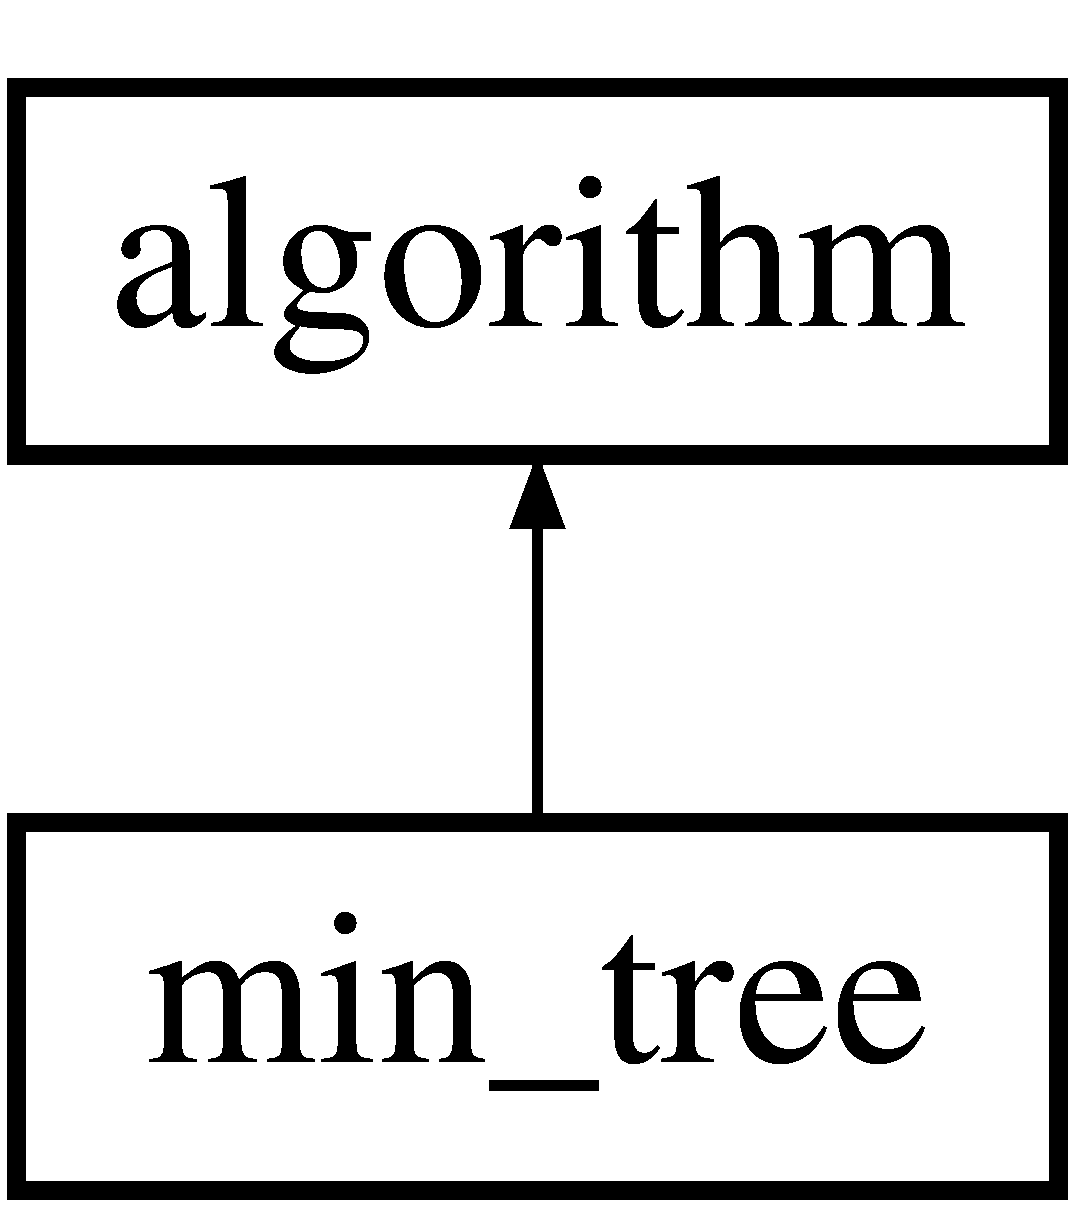
\includegraphics[height=2.000000cm]{classmin__tree}
\end{center}
\end{figure}
\subsection*{Public Member Functions}
\begin{DoxyCompactItemize}
\item 
\mbox{\Hypertarget{classmin__tree_a4be3e62d3ba8237883dcc04419ecd483}\label{classmin__tree_a4be3e62d3ba8237883dcc04419ecd483}} 
\mbox{\hyperlink{classmin__tree_a4be3e62d3ba8237883dcc04419ecd483}{min\+\_\+tree}} ()
\begin{DoxyCompactList}\small\item\em Constructor. \end{DoxyCompactList}\item 
\mbox{\Hypertarget{classmin__tree_a0df992f77a8656121777aa2c0380a67a}\label{classmin__tree_a0df992f77a8656121777aa2c0380a67a}} 
virtual \mbox{\hyperlink{classmin__tree_a0df992f77a8656121777aa2c0380a67a}{$\sim$min\+\_\+tree}} ()
\begin{DoxyCompactList}\small\item\em Destructor. \end{DoxyCompactList}\item 
int \mbox{\hyperlink{classmin__tree_ad87b1bfbc687ad943c07538fa0c3d270}{check}} (\mbox{\hyperlink{classgraph}{graph}} \&g)
\begin{DoxyCompactList}\small\item\em Checks whether algorithm can be applied. \end{DoxyCompactList}\item 
int \mbox{\hyperlink{classmin__tree_ac025e8dad0db7a6a1e0e7b476b547802}{run}} (\mbox{\hyperlink{classgraph}{graph}} \&g)
\begin{DoxyCompactList}\small\item\em Applies algorithm to graph g. \end{DoxyCompactList}\item 
virtual void \mbox{\hyperlink{classmin__tree_a0edbe612424dc5f4de4701b8fd0df931}{reset}} ()
\begin{DoxyCompactList}\small\item\em Resets algorithm. \end{DoxyCompactList}\item 
void \mbox{\hyperlink{classmin__tree_a0f3eb1714b7859576037cf4b991b16cb}{set\+\_\+distances}} (const \mbox{\hyperlink{classedge__map}{edge\+\_\+map}}$<$ int $>$ \&dist)
\begin{DoxyCompactList}\small\item\em Sets edge weights. \end{DoxyCompactList}\item 
set$<$ \mbox{\hyperlink{classedge}{edge}} $>$ \mbox{\hyperlink{classmin__tree_a9feda096e7c32a402fb91702ed3679fc}{get\+\_\+min\+\_\+tree}} ()
\begin{DoxyCompactList}\small\item\em Edges of minimal spanning tree calculated in the last call of \mbox{\hyperlink{classmin__tree_ac025e8dad0db7a6a1e0e7b476b547802}{min\+\_\+tree\+::run}}. \end{DoxyCompactList}\item 
int \mbox{\hyperlink{classmin__tree_a8ca03d32ba55a9eb20b52fcb0e6fa6a5}{get\+\_\+min\+\_\+tree\+\_\+length}} ()
\begin{DoxyCompactList}\small\item\em Weight of minimal spanning tree. \end{DoxyCompactList}\end{DoxyCompactItemize}
\subsection*{Additional Inherited Members}


\subsection{Detailed Description}
Kruskal\textquotesingle{}s algorithm for finding minimal spanning tree of a graph. 

\begin{DoxyAuthor}{Author}
Stf Kolev 
\end{DoxyAuthor}


\subsection{Member Function Documentation}
\mbox{\Hypertarget{classmin__tree_ad87b1bfbc687ad943c07538fa0c3d270}\label{classmin__tree_ad87b1bfbc687ad943c07538fa0c3d270}} 
\index{min\+\_\+tree@{min\+\_\+tree}!check@{check}}
\index{check@{check}!min\+\_\+tree@{min\+\_\+tree}}
\subsubsection{\texorpdfstring{check()}{check()}}
{\footnotesize\ttfamily int min\+\_\+tree\+::check (\begin{DoxyParamCaption}\item[{\mbox{\hyperlink{classgraph}{graph}} \&}]{g }\end{DoxyParamCaption})\hspace{0.3cm}{\ttfamily [virtual]}}



Checks whether algorithm can be applied. 

The graph must
\begin{DoxyItemize}
\item be undirected
\item be connected
\item have more than 2 nodes
\end{DoxyItemize}

Additionally the weights of the edges must have been set in advance using \mbox{\hyperlink{classmin__tree_a0f3eb1714b7859576037cf4b991b16cb}{min\+\_\+tree\+::set\+\_\+distances}}.


\begin{DoxyParams}{Parameters}
{\em g} & graph \\
\hline
\end{DoxyParams}
\begin{DoxyReturn}{Returns}
\mbox{\hyperlink{classalgorithm_af1a0078e153aa99c24f9bdf0d97f6710aae4c1cd7fe8d8cf4b143241a6e7c31cf}{algorithm\+::\+K\+G\+L\+\_\+\+OK}} if algorithm can be applied \mbox{\hyperlink{classalgorithm_af1a0078e153aa99c24f9bdf0d97f6710ae67bf27b2ef31f73e545a7f9f4a69556}{algorithm\+::\+K\+G\+L\+\_\+\+E\+R\+R\+OR}} otherwise. 
\end{DoxyReturn}


Implements \mbox{\hyperlink{classalgorithm_a76361fb03ad1cf643affc51821e43bed}{algorithm}}.

\mbox{\Hypertarget{classmin__tree_a9feda096e7c32a402fb91702ed3679fc}\label{classmin__tree_a9feda096e7c32a402fb91702ed3679fc}} 
\index{min\+\_\+tree@{min\+\_\+tree}!get\+\_\+min\+\_\+tree@{get\+\_\+min\+\_\+tree}}
\index{get\+\_\+min\+\_\+tree@{get\+\_\+min\+\_\+tree}!min\+\_\+tree@{min\+\_\+tree}}
\subsubsection{\texorpdfstring{get\+\_\+min\+\_\+tree()}{get\_min\_tree()}}
{\footnotesize\ttfamily set$<$ \mbox{\hyperlink{classedge}{edge}} $>$ min\+\_\+tree\+::get\+\_\+min\+\_\+tree (\begin{DoxyParamCaption}{ }\end{DoxyParamCaption})}



Edges of minimal spanning tree calculated in the last call of \mbox{\hyperlink{classmin__tree_ac025e8dad0db7a6a1e0e7b476b547802}{min\+\_\+tree\+::run}}. 

\begin{DoxyReturn}{Returns}
Set of edges of representing the minimal spanning tree 
\end{DoxyReturn}
\mbox{\Hypertarget{classmin__tree_a8ca03d32ba55a9eb20b52fcb0e6fa6a5}\label{classmin__tree_a8ca03d32ba55a9eb20b52fcb0e6fa6a5}} 
\index{min\+\_\+tree@{min\+\_\+tree}!get\+\_\+min\+\_\+tree\+\_\+length@{get\+\_\+min\+\_\+tree\+\_\+length}}
\index{get\+\_\+min\+\_\+tree\+\_\+length@{get\+\_\+min\+\_\+tree\+\_\+length}!min\+\_\+tree@{min\+\_\+tree}}
\subsubsection{\texorpdfstring{get\+\_\+min\+\_\+tree\+\_\+length()}{get\_min\_tree\_length()}}
{\footnotesize\ttfamily int min\+\_\+tree\+::get\+\_\+min\+\_\+tree\+\_\+length (\begin{DoxyParamCaption}{ }\end{DoxyParamCaption})}



Weight of minimal spanning tree. 

\begin{DoxyReturn}{Returns}
weight of minimal spanning tree. 
\end{DoxyReturn}
\mbox{\Hypertarget{classmin__tree_a0edbe612424dc5f4de4701b8fd0df931}\label{classmin__tree_a0edbe612424dc5f4de4701b8fd0df931}} 
\index{min\+\_\+tree@{min\+\_\+tree}!reset@{reset}}
\index{reset@{reset}!min\+\_\+tree@{min\+\_\+tree}}
\subsubsection{\texorpdfstring{reset()}{reset()}}
{\footnotesize\ttfamily void min\+\_\+tree\+::reset (\begin{DoxyParamCaption}{ }\end{DoxyParamCaption})\hspace{0.3cm}{\ttfamily [virtual]}}



Resets algorithm. 

Prepares the algorithm to be applied to another graph. {\itshape Please} {\itshape note\+:} The options an algorithm may support do {\itshape not} get reset by this. It is just to reset internally used datastructures. 

Implements \mbox{\hyperlink{classalgorithm_a21aba63d066ae7897de6ca7d8425c408}{algorithm}}.

\mbox{\Hypertarget{classmin__tree_ac025e8dad0db7a6a1e0e7b476b547802}\label{classmin__tree_ac025e8dad0db7a6a1e0e7b476b547802}} 
\index{min\+\_\+tree@{min\+\_\+tree}!run@{run}}
\index{run@{run}!min\+\_\+tree@{min\+\_\+tree}}
\subsubsection{\texorpdfstring{run()}{run()}}
{\footnotesize\ttfamily int min\+\_\+tree\+::run (\begin{DoxyParamCaption}\item[{\mbox{\hyperlink{classgraph}{graph}} \&}]{g }\end{DoxyParamCaption})\hspace{0.3cm}{\ttfamily [virtual]}}



Applies algorithm to graph g. 


\begin{DoxyParams}{Parameters}
{\em g} & graph \\
\hline
\end{DoxyParams}

\begin{DoxyRetVals}{Return values}
{\em \mbox{\hyperlink{classalgorithm_af1a0078e153aa99c24f9bdf0d97f6710aae4c1cd7fe8d8cf4b143241a6e7c31cf}{algorithm\+::\+K\+G\+L\+\_\+\+OK}}} & on success \\
\hline
{\em \mbox{\hyperlink{classalgorithm_af1a0078e153aa99c24f9bdf0d97f6710ae67bf27b2ef31f73e545a7f9f4a69556}{algorithm\+::\+K\+G\+L\+\_\+\+E\+R\+R\+OR}}} & otherwise \\
\hline
\end{DoxyRetVals}


Implements \mbox{\hyperlink{classalgorithm_a734b189509a8d6b56b65f8ff772d43ca}{algorithm}}.

\mbox{\Hypertarget{classmin__tree_a0f3eb1714b7859576037cf4b991b16cb}\label{classmin__tree_a0f3eb1714b7859576037cf4b991b16cb}} 
\index{min\+\_\+tree@{min\+\_\+tree}!set\+\_\+distances@{set\+\_\+distances}}
\index{set\+\_\+distances@{set\+\_\+distances}!min\+\_\+tree@{min\+\_\+tree}}
\subsubsection{\texorpdfstring{set\+\_\+distances()}{set\_distances()}}
{\footnotesize\ttfamily void min\+\_\+tree\+::set\+\_\+distances (\begin{DoxyParamCaption}\item[{const \mbox{\hyperlink{classedge__map}{edge\+\_\+map}}$<$ int $>$ \&}]{dist }\end{DoxyParamCaption})}



Sets edge weights. 

Setting of edge weights must be done before calling \mbox{\hyperlink{classmin__tree_ad87b1bfbc687ad943c07538fa0c3d270}{min\+\_\+tree\+::check}} and \mbox{\hyperlink{classmin__tree_ac025e8dad0db7a6a1e0e7b476b547802}{min\+\_\+tree\+::run}}.


\begin{DoxyParams}{Parameters}
{\em dist} & edge weigths. \\
\hline
\end{DoxyParams}


The documentation for this class was generated from the following files\+:\begin{DoxyCompactItemize}
\item 
include/\+K\+G\+L/min\+\_\+tree.\+h\item 
src/min\+\_\+tree.\+cpp\end{DoxyCompactItemize}

\hypertarget{classne__map}{}\section{ne\+\_\+map$<$ Key, Value, Graph, Alloc $>$ Class Template Reference}
\label{classne__map}\index{ne\+\_\+map$<$ Key, Value, Graph, Alloc $>$@{ne\+\_\+map$<$ Key, Value, Graph, Alloc $>$}}


Baseclass for \mbox{\hyperlink{classnode__map}{node\+\_\+map}} and \mbox{\hyperlink{classedge__map}{edge\+\_\+map}}.  




{\ttfamily \#include $<$ne\+\_\+map.\+h$>$}

\subsection*{Public Types}
\begin{DoxyCompactItemize}
\item 
\mbox{\Hypertarget{classne__map_afd021ff2dd14cd255ec0635af1acde8a}\label{classne__map_afd021ff2dd14cd255ec0635af1acde8a}} 
typedef vector$<$ Value, Alloc $>$\+::reference {\bfseries value\+\_\+reference}
\item 
\mbox{\Hypertarget{classne__map_aab434040b52c0b0477cdfa4639869523}\label{classne__map_aab434040b52c0b0477cdfa4639869523}} 
typedef vector$<$ Value, Alloc $>$\+::const\+\_\+reference {\bfseries const\+\_\+value\+\_\+reference}
\end{DoxyCompactItemize}
\subsection*{Public Member Functions}
\begin{DoxyCompactItemize}
\item 
void \mbox{\hyperlink{classne__map_a4ef2ab4aebcb57a7a101975bf6a88e24}{init}} (const Graph \&, Value def=Value())
\item 
value\+\_\+reference \mbox{\hyperlink{classne__map_a4bcfa7ec2dcbfaa42fab93dfa81e8ab0}{operator\mbox{[}$\,$\mbox{]}}} (Key key)
\item 
const\+\_\+value\+\_\+reference \mbox{\hyperlink{classne__map_ad8d23cc924963ddff8267e625dcbffc6}{operator\mbox{[}$\,$\mbox{]}}} (Key key) const
\item 
void \mbox{\hyperlink{classne__map_aebe555c23769c6dcc869b5ac7fae6a9c}{clear}} ()
\end{DoxyCompactItemize}
\subsection*{Protected Member Functions}
\begin{DoxyCompactItemize}
\item 
\mbox{\hyperlink{classne__map_acbe94c2209408e8af27fb9580251f360}{ne\+\_\+map}} ()
\item 
\mbox{\hyperlink{classne__map_a769ee373d4cd8d3ef2c1577372da149c}{ne\+\_\+map}} (const Graph \&g, Value def=Value())
\end{DoxyCompactItemize}


\subsection{Detailed Description}
\subsubsection*{template$<$class Key, class Value, class Graph, class Alloc = allocator$<$\+Value$>$$>$\newline
class ne\+\_\+map$<$ Key, Value, Graph, Alloc $>$}

Baseclass for \mbox{\hyperlink{classnode__map}{node\+\_\+map}} and \mbox{\hyperlink{classedge__map}{edge\+\_\+map}}. 

\mbox{\hyperlink{classne__map}{ne\+\_\+map}} is the common implementation of {\ttfamily \mbox{\hyperlink{classnode__map}{node\+\_\+map}} } and {\ttfamily \mbox{\hyperlink{classedge__map}{edge\+\_\+map}} } and cannot be used directly. 

\subsection{Constructor \& Destructor Documentation}
\mbox{\Hypertarget{classne__map_acbe94c2209408e8af27fb9580251f360}\label{classne__map_acbe94c2209408e8af27fb9580251f360}} 
\index{ne\+\_\+map@{ne\+\_\+map}!ne\+\_\+map@{ne\+\_\+map}}
\index{ne\+\_\+map@{ne\+\_\+map}!ne\+\_\+map@{ne\+\_\+map}}
\subsubsection{\texorpdfstring{ne\+\_\+map()}{ne\_map()}\hspace{0.1cm}{\footnotesize\ttfamily [1/2]}}
{\footnotesize\ttfamily template$<$class Key , class Value , class Graph , class Alloc $>$ \\
\mbox{\hyperlink{classne__map}{ne\+\_\+map}}$<$ Key, Value, Graph, Alloc $>$\+::\mbox{\hyperlink{classne__map}{ne\+\_\+map}} (\begin{DoxyParamCaption}{ }\end{DoxyParamCaption})\hspace{0.3cm}{\ttfamily [protected]}}

Constructs an empty {\ttfamily \mbox{\hyperlink{classne__map}{ne\+\_\+map}}} not associated to any {\ttfamily graph}. \mbox{\Hypertarget{classne__map_a769ee373d4cd8d3ef2c1577372da149c}\label{classne__map_a769ee373d4cd8d3ef2c1577372da149c}} 
\index{ne\+\_\+map@{ne\+\_\+map}!ne\+\_\+map@{ne\+\_\+map}}
\index{ne\+\_\+map@{ne\+\_\+map}!ne\+\_\+map@{ne\+\_\+map}}
\subsubsection{\texorpdfstring{ne\+\_\+map()}{ne\_map()}\hspace{0.1cm}{\footnotesize\ttfamily [2/2]}}
{\footnotesize\ttfamily template$<$class Key , class Value, class Graph, class Alloc $>$ \\
\mbox{\hyperlink{classne__map}{ne\+\_\+map}}$<$ Key, Value, Graph, Alloc $>$\+::\mbox{\hyperlink{classne__map}{ne\+\_\+map}} (\begin{DoxyParamCaption}\item[{const Graph \&}]{g,  }\item[{Value}]{def = {\ttfamily Value()} }\end{DoxyParamCaption})\hspace{0.3cm}{\ttfamily [explicit]}, {\ttfamily [protected]}}

Constructs a {\ttfamily \mbox{\hyperlink{classne__map}{ne\+\_\+map}}} associated to the {\ttfamily graph g}. The value associated to each key is set to {\ttfamily def}. You may (but need not) call {\ttfamily ne\+\_\+map\+::init(const graph \&, T)} to associate it to a {\ttfamily graph}.


\begin{DoxyParams}{Parameters}
{\em $<$code$>$g$<$/code$>$} & associated {\ttfamily graph} \\
\hline
{\em $<$code$>$def$<$/code$>$} & default value \\
\hline
\end{DoxyParams}


\subsection{Member Function Documentation}
\mbox{\Hypertarget{classne__map_aebe555c23769c6dcc869b5ac7fae6a9c}\label{classne__map_aebe555c23769c6dcc869b5ac7fae6a9c}} 
\index{ne\+\_\+map@{ne\+\_\+map}!clear@{clear}}
\index{clear@{clear}!ne\+\_\+map@{ne\+\_\+map}}
\subsubsection{\texorpdfstring{clear()}{clear()}}
{\footnotesize\ttfamily template$<$class Key , class Value , class Graph , class Alloc $>$ \\
void \mbox{\hyperlink{classne__map}{ne\+\_\+map}}$<$ Key, Value, Graph, Alloc $>$\+::clear (\begin{DoxyParamCaption}{ }\end{DoxyParamCaption})}

Erases a elements of this nodemap \mbox{\Hypertarget{classne__map_a4ef2ab4aebcb57a7a101975bf6a88e24}\label{classne__map_a4ef2ab4aebcb57a7a101975bf6a88e24}} 
\index{ne\+\_\+map@{ne\+\_\+map}!init@{init}}
\index{init@{init}!ne\+\_\+map@{ne\+\_\+map}}
\subsubsection{\texorpdfstring{init()}{init()}}
{\footnotesize\ttfamily template$<$class Key , class Value, class Graph, class Alloc $>$ \\
void \mbox{\hyperlink{classne__map}{ne\+\_\+map}}$<$ Key, Value, Graph, Alloc $>$\+::init (\begin{DoxyParamCaption}\item[{const Graph \&}]{g,  }\item[{Value}]{def = {\ttfamily Value()} }\end{DoxyParamCaption})}

Initializes the \mbox{\hyperlink{classne__map}{ne\+\_\+map}} to hold information for the elements of graph g. def is the value associated with all elements.


\begin{DoxyParams}{Parameters}
{\em $<$code$>$g$<$/code$>$} & associated {\ttfamily graph} \\
\hline
{\em $<$code$>$def$<$/code$>$} & default value \\
\hline
\end{DoxyParams}
\mbox{\Hypertarget{classne__map_a4bcfa7ec2dcbfaa42fab93dfa81e8ab0}\label{classne__map_a4bcfa7ec2dcbfaa42fab93dfa81e8ab0}} 
\index{ne\+\_\+map@{ne\+\_\+map}!operator\mbox{[}\mbox{]}@{operator[]}}
\index{operator\mbox{[}\mbox{]}@{operator[]}!ne\+\_\+map@{ne\+\_\+map}}
\subsubsection{\texorpdfstring{operator[]()}{operator[]()}\hspace{0.1cm}{\footnotesize\ttfamily [1/2]}}
{\footnotesize\ttfamily template$<$class Key, class Value , class Graph , class Alloc $>$ \\
\mbox{\hyperlink{classne__map}{ne\+\_\+map}}$<$ Key, Value, Graph, Alloc $>$\+::value\+\_\+reference \mbox{\hyperlink{classne__map}{ne\+\_\+map}}$<$ Key, Value, Graph, Alloc $>$\+::operator\mbox{[}$\,$\mbox{]} (\begin{DoxyParamCaption}\item[{Key}]{key }\end{DoxyParamCaption})}

Read/write accessor function to the value associated with {\ttfamily key}. Use this function to change the value of an element in the {\ttfamily \mbox{\hyperlink{classne__map}{ne\+\_\+map}}}. Assume that {\ttfamily ne} is a {\ttfamily \mbox{\hyperlink{classne__map}{ne\+\_\+map}}$<$int$>$}. Then you can assign the value 5 to {\ttfamily key} with\+: 
\begin{DoxyPre}
  ne[key] = 5;
\end{DoxyPre}


If there is no entry in the {\ttfamily \mbox{\hyperlink{classne__map}{ne\+\_\+map}}} associated with {\ttfamily key}, one is created.


\begin{DoxyParams}{Parameters}
{\em key} & Key of the Entry to change \\
\hline
\end{DoxyParams}
\begin{DoxyReturn}{Returns}
a reference to the value associated to {\ttfamily key}. 
\end{DoxyReturn}
\mbox{\Hypertarget{classne__map_ad8d23cc924963ddff8267e625dcbffc6}\label{classne__map_ad8d23cc924963ddff8267e625dcbffc6}} 
\index{ne\+\_\+map@{ne\+\_\+map}!operator\mbox{[}\mbox{]}@{operator[]}}
\index{operator\mbox{[}\mbox{]}@{operator[]}!ne\+\_\+map@{ne\+\_\+map}}
\subsubsection{\texorpdfstring{operator[]()}{operator[]()}\hspace{0.1cm}{\footnotesize\ttfamily [2/2]}}
{\footnotesize\ttfamily template$<$class Key, class Value , class Graph , class Alloc $>$ \\
\mbox{\hyperlink{classne__map}{ne\+\_\+map}}$<$ Key, Value, Graph, Alloc $>$\+::const\+\_\+value\+\_\+reference \mbox{\hyperlink{classne__map}{ne\+\_\+map}}$<$ Key, Value, Graph, Alloc $>$\+::operator\mbox{[}$\,$\mbox{]} (\begin{DoxyParamCaption}\item[{Key}]{key }\end{DoxyParamCaption}) const}

Read-\/only accessor function to the value associated with {\ttfamily key}. Use this function to read the value of an element in the {\ttfamily \mbox{\hyperlink{classne__map}{ne\+\_\+map}}}. Assume that {\ttfamily ne} is a {\ttfamily \mbox{\hyperlink{classne__map}{ne\+\_\+map}}$<$int$>$}. Then you can print the value associated with {\ttfamily key} with\+: 
\begin{DoxyPre}
  cout << ne[key];
\end{DoxyPre}



\begin{DoxyParams}{Parameters}
{\em key} & Key of the Entry to look up \\
\hline
\end{DoxyParams}
\begin{DoxyReturn}{Returns}
a const reference to the value associated to {\ttfamily key}. 
\end{DoxyReturn}


The documentation for this class was generated from the following file\+:\begin{DoxyCompactItemize}
\item 
include/\+K\+G\+L/ne\+\_\+map.\+h\end{DoxyCompactItemize}

\hypertarget{classnode}{}\section{node Class Reference}
\label{classnode}\index{node@{node}}


A node in a graph.  




{\ttfamily \#include $<$node.\+h$>$}

Inheritance diagram for node\+:\begin{figure}[H]
\begin{center}
\leavevmode
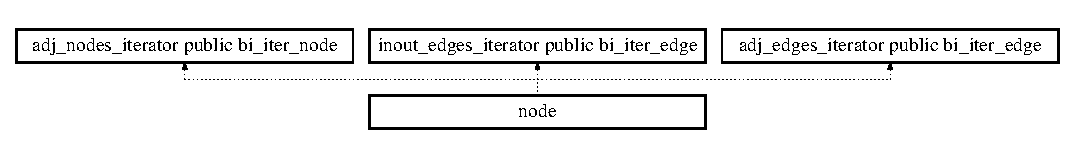
\includegraphics[height=1.499331cm]{classnode}
\end{center}
\end{figure}
\subsection*{Public Types}
\begin{DoxyCompactItemize}
\item 
\mbox{\Hypertarget{classnode_a3576579529747e88ab7d1a8ba3122f2e}\label{classnode_a3576579529747e88ab7d1a8ba3122f2e}} 
typedef list$<$ \mbox{\hyperlink{classedge}{edge}} $>$\+::const\+\_\+iterator {\bfseries in\+\_\+edges\+\_\+iterator}
\item 
\mbox{\Hypertarget{classnode_a4715326ede44c91e24aba42f49089da4}\label{classnode_a4715326ede44c91e24aba42f49089da4}} 
typedef list$<$ \mbox{\hyperlink{classedge}{edge}} $>$\+::const\+\_\+iterator {\bfseries out\+\_\+edges\+\_\+iterator}
\end{DoxyCompactItemize}
\subsection*{Public Member Functions}
\begin{DoxyCompactItemize}
\item 
\mbox{\hyperlink{classnode_ad603259398d5667e3b97a6322a2bcc20}{node}} ()
\item 
int \mbox{\hyperlink{classnode_a1e5e94e426da180a069cf307616e38e3}{degree}} () const
\item 
int \mbox{\hyperlink{classnode_a32adc45c4132e2642ccd2233d79ffe67}{outdeg}} () const
\item 
int \mbox{\hyperlink{classnode_a749bfd1316584b96f8c9b0e44ad512f0}{indeg}} () const
\item 
\mbox{\Hypertarget{classnode_a5d38b4152c3cedb235e45de7eb3f4469}\label{classnode_a5d38b4152c3cedb235e45de7eb3f4469}} 
int {\bfseries id} () const
\item 
const \mbox{\hyperlink{classnode}{node}} \& \mbox{\hyperlink{classnode_a13dbd1809a33a5efede64a359e53a363}{opposite}} (\mbox{\hyperlink{classedge}{edge}} e) const
\item 
\mbox{\Hypertarget{classnode_aa27614c7a557ea4b5b1d621c887e3ca5}\label{classnode_aa27614c7a557ea4b5b1d621c887e3ca5}} 
list$<$ \mbox{\hyperlink{classnode}{node}} $>$ {\bfseries opposites} (\mbox{\hyperlink{classedge}{edge}}) const
\item 
bool \mbox{\hyperlink{classnode_af948e15fd00a31e67928c9061acda582}{is\+\_\+hidden}} () const
\item 
int \mbox{\hyperlink{classnode_aba6b3a48e7b951f08ebbbf3275f0ce9a}{excentricity}} () const
\item 
adj\+\_\+nodes\+\_\+iterator \mbox{\hyperlink{classnode_a6cd2febf910bc6572c4aecba6278b100}{adj\+\_\+nodes\+\_\+begin}} () const
\item 
adj\+\_\+nodes\+\_\+iterator \mbox{\hyperlink{classnode_a2477fa92c56a19d29464082444a3043a}{adj\+\_\+nodes\+\_\+end}} () const
\item 
adj\+\_\+edges\+\_\+iterator \mbox{\hyperlink{classnode_a788d3e932a5c164caa5ec82aa47551b2}{adj\+\_\+edges\+\_\+begin}} () const
\item 
adj\+\_\+edges\+\_\+iterator \mbox{\hyperlink{classnode_aa1e7887d29390297580769454f769ad6}{adj\+\_\+edges\+\_\+end}} () const
\item 
in\+\_\+edges\+\_\+iterator \mbox{\hyperlink{classnode_a0c32377f370ae52ed2134ff8d4dac584}{in\+\_\+edges\+\_\+begin}} () const
\item 
in\+\_\+edges\+\_\+iterator \mbox{\hyperlink{classnode_a785cd330f8b4c5c47d3b6e936a7e744e}{in\+\_\+edges\+\_\+end}} () const
\item 
out\+\_\+edges\+\_\+iterator \mbox{\hyperlink{classnode_a7dcb80df22118cea04f77ca8c952d9c2}{out\+\_\+edges\+\_\+begin}} () const
\item 
out\+\_\+edges\+\_\+iterator \mbox{\hyperlink{classnode_a7ce2ba5195a63d4df6b44299a02a9378}{out\+\_\+edges\+\_\+end}} () const
\item 
inout\+\_\+edges\+\_\+iterator \mbox{\hyperlink{classnode_a8677f4dc2acfb64310de1ea866c17340}{inout\+\_\+edges\+\_\+begin}} () const
\item 
inout\+\_\+edges\+\_\+iterator \mbox{\hyperlink{classnode_ad4eec3efcc3c1e572b0492276e20980c}{inout\+\_\+edges\+\_\+end}} () const
\item 
\mbox{\Hypertarget{classnode_a12cb1a2167f5f03c054de5e707d3156f}\label{classnode_a12cb1a2167f5f03c054de5e707d3156f}} 
{\bfseries adj\+\_\+edges\+\_\+iterator} ()
\item 
\mbox{\Hypertarget{classnode_a1b7aa43ddd3e7f392479c479400ebb75}\label{classnode_a1b7aa43ddd3e7f392479c479400ebb75}} 
{\bfseries adj\+\_\+edges\+\_\+iterator} (\mbox{\hyperlink{classnode}{node}}, bool)
\item 
\mbox{\Hypertarget{classnode_a7ae20e73507364af0c1df22ecd0df444}\label{classnode_a7ae20e73507364af0c1df22ecd0df444}} 
bool {\bfseries operator==} (const adj\+\_\+edges\+\_\+iterator \&) const
\item 
\mbox{\Hypertarget{classnode_aa30fcffcf193cc94d3e1f3fe419ce42a}\label{classnode_aa30fcffcf193cc94d3e1f3fe419ce42a}} 
bool {\bfseries operator!=} (const adj\+\_\+edges\+\_\+iterator \&) const
\item 
\mbox{\Hypertarget{classnode_a5849d021a696f38d1b2e1d3d3372bbe7}\label{classnode_a5849d021a696f38d1b2e1d3d3372bbe7}} 
adj\+\_\+edges\+\_\+iterator \& {\bfseries operator++} ()
\item 
\mbox{\Hypertarget{classnode_ac112a3065e69e4897d38c11980fe1789}\label{classnode_ac112a3065e69e4897d38c11980fe1789}} 
adj\+\_\+edges\+\_\+iterator {\bfseries operator++} (int)
\item 
\mbox{\Hypertarget{classnode_a99fdb299b044facd9cb3f90f18a559fd}\label{classnode_a99fdb299b044facd9cb3f90f18a559fd}} 
adj\+\_\+edges\+\_\+iterator \& {\bfseries operator-\/-\/} ()
\item 
\mbox{\Hypertarget{classnode_a1e5751de7ba220836ffee941707c277b}\label{classnode_a1e5751de7ba220836ffee941707c277b}} 
adj\+\_\+edges\+\_\+iterator {\bfseries operator-\/-\/} (int)
\item 
\mbox{\Hypertarget{classnode_a914c034c6f43029ad9b7f0826dd2614f}\label{classnode_a914c034c6f43029ad9b7f0826dd2614f}} 
const \mbox{\hyperlink{classedge}{edge}} \& {\bfseries operator$\ast$} () const
\item 
\mbox{\Hypertarget{classnode_a71b168f27cc7338906814f6a3ecc176f}\label{classnode_a71b168f27cc7338906814f6a3ecc176f}} 
const \mbox{\hyperlink{classedge}{edge}} $\ast$ {\bfseries operator-\/$>$} () const
\item 
\mbox{\Hypertarget{classnode_a854d596611e6a3342090cce71cedf300}\label{classnode_a854d596611e6a3342090cce71cedf300}} 
{\bfseries inout\+\_\+edges\+\_\+iterator} ()
\item 
\mbox{\Hypertarget{classnode_a2990a550ae39da89f6d18e6b5faf519e}\label{classnode_a2990a550ae39da89f6d18e6b5faf519e}} 
{\bfseries inout\+\_\+edges\+\_\+iterator} (\mbox{\hyperlink{classnode}{node}} n, bool start)
\item 
\mbox{\Hypertarget{classnode_ae6b790b8b1dd9733be73b1d2c84716df}\label{classnode_ae6b790b8b1dd9733be73b1d2c84716df}} 
bool {\bfseries operator==} (const inout\+\_\+edges\+\_\+iterator \&) const
\item 
\mbox{\Hypertarget{classnode_ac4efb2e8423b3502f9d3a1bd6de80e73}\label{classnode_ac4efb2e8423b3502f9d3a1bd6de80e73}} 
bool {\bfseries operator!=} (const inout\+\_\+edges\+\_\+iterator \&) const
\item 
\mbox{\Hypertarget{classnode_a934fd5ac6865ae23f3b2758a573550ec}\label{classnode_a934fd5ac6865ae23f3b2758a573550ec}} 
inout\+\_\+edges\+\_\+iterator \& {\bfseries operator++} ()
\item 
\mbox{\Hypertarget{classnode_a754f5fcf2ab3d5bf26e1e4fdc47cc766}\label{classnode_a754f5fcf2ab3d5bf26e1e4fdc47cc766}} 
inout\+\_\+edges\+\_\+iterator {\bfseries operator++} (int)
\item 
\mbox{\Hypertarget{classnode_a046088eba56244e29945d0197f6b642f}\label{classnode_a046088eba56244e29945d0197f6b642f}} 
inout\+\_\+edges\+\_\+iterator \& {\bfseries operator-\/-\/} ()
\item 
\mbox{\Hypertarget{classnode_a9b906907ed01bb04c06bed300428da11}\label{classnode_a9b906907ed01bb04c06bed300428da11}} 
inout\+\_\+edges\+\_\+iterator {\bfseries operator-\/-\/} (int)
\item 
\mbox{\Hypertarget{classnode_a914c034c6f43029ad9b7f0826dd2614f}\label{classnode_a914c034c6f43029ad9b7f0826dd2614f}} 
const \mbox{\hyperlink{classedge}{edge}} \& {\bfseries operator$\ast$} () const
\item 
\mbox{\Hypertarget{classnode_a71b168f27cc7338906814f6a3ecc176f}\label{classnode_a71b168f27cc7338906814f6a3ecc176f}} 
const \mbox{\hyperlink{classedge}{edge}} $\ast$ {\bfseries operator-\/$>$} () const
\item 
\mbox{\Hypertarget{classnode_a392f19ea6dfa344bdf5c4d5a4b25eb8c}\label{classnode_a392f19ea6dfa344bdf5c4d5a4b25eb8c}} 
{\bfseries adj\+\_\+nodes\+\_\+iterator} ()
\item 
\mbox{\Hypertarget{classnode_ade9ca1b2c63a0467be176756545b3c2c}\label{classnode_ade9ca1b2c63a0467be176756545b3c2c}} 
{\bfseries adj\+\_\+nodes\+\_\+iterator} (const \mbox{\hyperlink{classnode}{node}} \&, bool)
\item 
\mbox{\Hypertarget{classnode_abe20131c7427c6f045ab4c23916efa3c}\label{classnode_abe20131c7427c6f045ab4c23916efa3c}} 
bool {\bfseries operator==} (const adj\+\_\+nodes\+\_\+iterator \&) const
\item 
\mbox{\Hypertarget{classnode_abfcd7e8ce1391bd60f155a5de47419c5}\label{classnode_abfcd7e8ce1391bd60f155a5de47419c5}} 
bool {\bfseries operator!=} (const adj\+\_\+nodes\+\_\+iterator \&) const
\item 
\mbox{\Hypertarget{classnode_a5c9569e6719a8bebd6dd78266a0da533}\label{classnode_a5c9569e6719a8bebd6dd78266a0da533}} 
adj\+\_\+nodes\+\_\+iterator \& {\bfseries operator++} ()
\item 
\mbox{\Hypertarget{classnode_af12ab69bcd07d4d41052b50801690520}\label{classnode_af12ab69bcd07d4d41052b50801690520}} 
adj\+\_\+nodes\+\_\+iterator {\bfseries operator++} (int)
\item 
\mbox{\Hypertarget{classnode_abd4b60efd003b18db13d9fde0a25f91a}\label{classnode_abd4b60efd003b18db13d9fde0a25f91a}} 
adj\+\_\+nodes\+\_\+iterator \& {\bfseries operator-\/-\/} ()
\item 
\mbox{\Hypertarget{classnode_ae7cdb2be553782c2dcf48c6ec8ef9d67}\label{classnode_ae7cdb2be553782c2dcf48c6ec8ef9d67}} 
adj\+\_\+nodes\+\_\+iterator {\bfseries operator-\/-\/} (int)
\item 
\mbox{\Hypertarget{classnode_a59fdf9aff393a47b4c60c3f21a4ccbc8}\label{classnode_a59fdf9aff393a47b4c60c3f21a4ccbc8}} 
const \mbox{\hyperlink{classnode}{node}} \& {\bfseries operator$\ast$} () const
\item 
\mbox{\Hypertarget{classnode_a82d46c8753db26b34382fcfd9f887c12}\label{classnode_a82d46c8753db26b34382fcfd9f887c12}} 
const \mbox{\hyperlink{classnode}{node}} $\ast$ {\bfseries operator-\/$>$} () const
\end{DoxyCompactItemize}
\subsection*{Friends}
\begin{DoxyCompactItemize}
\item 
\mbox{\Hypertarget{classnode_ab8b0dbc1b36724e5e4635ac651c218cb}\label{classnode_ab8b0dbc1b36724e5e4635ac651c218cb}} 
class {\bfseries graph}
\item 
\mbox{\Hypertarget{classnode_a534891c80172dde5e777a3908cc6e2f1}\label{classnode_a534891c80172dde5e777a3908cc6e2f1}} 
class {\bfseries edge}
\item 
\mbox{\Hypertarget{classnode_abdd49248203010f2d5432dfef22d017a}\label{classnode_abdd49248203010f2d5432dfef22d017a}} 
class {\bfseries adj\+\_\+edges\+\_\+iterator}
\item 
\mbox{\Hypertarget{classnode_a19ea521fd5b3813e179997758f1109f0}\label{classnode_a19ea521fd5b3813e179997758f1109f0}} 
K\+G\+L\+\_\+\+E\+X\+T\+E\+RN friend bool {\bfseries operator==} (\mbox{\hyperlink{classnode}{node}}, \mbox{\hyperlink{classnode}{node}})
\item 
\mbox{\Hypertarget{classnode_ac95f53a475a3895dff3f9495ab87bf75}\label{classnode_ac95f53a475a3895dff3f9495ab87bf75}} 
K\+G\+L\+\_\+\+E\+X\+T\+E\+RN friend bool {\bfseries operator!=} (\mbox{\hyperlink{classnode}{node}}, \mbox{\hyperlink{classnode}{node}})
\item 
\mbox{\Hypertarget{classnode_a01896810a81fff14def134f6e9638f99}\label{classnode_a01896810a81fff14def134f6e9638f99}} 
K\+G\+L\+\_\+\+E\+X\+T\+E\+RN friend bool {\bfseries operator$<$} (\mbox{\hyperlink{classnode}{node}}, \mbox{\hyperlink{classnode}{node}})
\item 
\mbox{\Hypertarget{classnode_a6252a93f7623a3554f5b877874639f4e}\label{classnode_a6252a93f7623a3554f5b877874639f4e}} 
K\+G\+L\+\_\+\+E\+X\+T\+E\+RN friend ostream \& {\bfseries operator$<$$<$} (ostream \&os, const \mbox{\hyperlink{classnode}{node}} \&n)
\end{DoxyCompactItemize}


\subsection{Detailed Description}
A node in a graph. 

Iterator for adjacent nodes of a node.

Iterator for all incident edges of a node.

Iterator for adjacent edges of a node. 

\subsection{Constructor \& Destructor Documentation}
\mbox{\Hypertarget{classnode_ad603259398d5667e3b97a6322a2bcc20}\label{classnode_ad603259398d5667e3b97a6322a2bcc20}} 
\index{node@{node}!node@{node}}
\index{node@{node}!node@{node}}
\subsubsection{\texorpdfstring{node()}{node()}}
{\footnotesize\ttfamily \+\_\+\+\_\+\+K\+G\+L\+\_\+\+B\+E\+G\+I\+N\+\_\+\+N\+A\+M\+E\+S\+P\+A\+CE node\+::node (\begin{DoxyParamCaption}{ }\end{DoxyParamCaption})}

Default constructor. Creates an invalid node. The only way to obtain a valid node is through \mbox{\hyperlink{classgraph_ab9505335c20558319b6cce25aed23524}{graph\+::new\+\_\+node}} Example\+: 
\begin{DoxyPre}
  graph g;
  node n;\end{DoxyPre}



\begin{DoxyPre}  n = g.new\_node();
\end{DoxyPre}


\begin{DoxySeeAlso}{See also}
\mbox{\hyperlink{classgraph_ab9505335c20558319b6cce25aed23524}{graph\+::new\+\_\+node}} 
\end{DoxySeeAlso}


\subsection{Member Function Documentation}
\mbox{\Hypertarget{classnode_a788d3e932a5c164caa5ec82aa47551b2}\label{classnode_a788d3e932a5c164caa5ec82aa47551b2}} 
\index{node@{node}!adj\+\_\+edges\+\_\+begin@{adj\+\_\+edges\+\_\+begin}}
\index{adj\+\_\+edges\+\_\+begin@{adj\+\_\+edges\+\_\+begin}!node@{node}}
\subsubsection{\texorpdfstring{adj\+\_\+edges\+\_\+begin()}{adj\_edges\_begin()}}
{\footnotesize\ttfamily node\+::adj\+\_\+edges\+\_\+iterator node\+::adj\+\_\+edges\+\_\+begin (\begin{DoxyParamCaption}{ }\end{DoxyParamCaption}) const}

Iterate through all adjacent edges.

\begin{DoxyReturn}{Returns}
start for iteration through all adjacent edges 
\end{DoxyReturn}
\mbox{\Hypertarget{classnode_aa1e7887d29390297580769454f769ad6}\label{classnode_aa1e7887d29390297580769454f769ad6}} 
\index{node@{node}!adj\+\_\+edges\+\_\+end@{adj\+\_\+edges\+\_\+end}}
\index{adj\+\_\+edges\+\_\+end@{adj\+\_\+edges\+\_\+end}!node@{node}}
\subsubsection{\texorpdfstring{adj\+\_\+edges\+\_\+end()}{adj\_edges\_end()}}
{\footnotesize\ttfamily node\+::adj\+\_\+edges\+\_\+iterator node\+::adj\+\_\+edges\+\_\+end (\begin{DoxyParamCaption}{ }\end{DoxyParamCaption}) const}

Iterate through all adjacent edges.

\begin{DoxyReturn}{Returns}
end for iteration through all adjacent edges 
\end{DoxyReturn}
\mbox{\Hypertarget{classnode_a6cd2febf910bc6572c4aecba6278b100}\label{classnode_a6cd2febf910bc6572c4aecba6278b100}} 
\index{node@{node}!adj\+\_\+nodes\+\_\+begin@{adj\+\_\+nodes\+\_\+begin}}
\index{adj\+\_\+nodes\+\_\+begin@{adj\+\_\+nodes\+\_\+begin}!node@{node}}
\subsubsection{\texorpdfstring{adj\+\_\+nodes\+\_\+begin()}{adj\_nodes\_begin()}}
{\footnotesize\ttfamily node\+::adj\+\_\+nodes\+\_\+iterator node\+::adj\+\_\+nodes\+\_\+begin (\begin{DoxyParamCaption}{ }\end{DoxyParamCaption}) const}

Iterate through all adjacent nodes.

\begin{DoxyReturn}{Returns}
start for iteration through all adjacent nodes 
\end{DoxyReturn}
\mbox{\Hypertarget{classnode_a2477fa92c56a19d29464082444a3043a}\label{classnode_a2477fa92c56a19d29464082444a3043a}} 
\index{node@{node}!adj\+\_\+nodes\+\_\+end@{adj\+\_\+nodes\+\_\+end}}
\index{adj\+\_\+nodes\+\_\+end@{adj\+\_\+nodes\+\_\+end}!node@{node}}
\subsubsection{\texorpdfstring{adj\+\_\+nodes\+\_\+end()}{adj\_nodes\_end()}}
{\footnotesize\ttfamily node\+::adj\+\_\+nodes\+\_\+iterator node\+::adj\+\_\+nodes\+\_\+end (\begin{DoxyParamCaption}{ }\end{DoxyParamCaption}) const}

Iterate through all adjacent nodes.

\begin{DoxyReturn}{Returns}
end for iteration through all adjacent nodes 
\end{DoxyReturn}
\mbox{\Hypertarget{classnode_a1e5e94e426da180a069cf307616e38e3}\label{classnode_a1e5e94e426da180a069cf307616e38e3}} 
\index{node@{node}!degree@{degree}}
\index{degree@{degree}!node@{node}}
\subsubsection{\texorpdfstring{degree()}{degree()}}
{\footnotesize\ttfamily int node\+::degree (\begin{DoxyParamCaption}{ }\end{DoxyParamCaption}) const}

Returns the degree of the node, i. e. \mbox{\hyperlink{classnode_a32adc45c4132e2642ccd2233d79ffe67}{node\+::outdeg}} + \mbox{\hyperlink{classnode_a749bfd1316584b96f8c9b0e44ad512f0}{node\+::indeg}} . \mbox{\Hypertarget{classnode_aba6b3a48e7b951f08ebbbf3275f0ce9a}\label{classnode_aba6b3a48e7b951f08ebbbf3275f0ce9a}} 
\index{node@{node}!excentricity@{excentricity}}
\index{excentricity@{excentricity}!node@{node}}
\subsubsection{\texorpdfstring{excentricity()}{excentricity()}}
{\footnotesize\ttfamily int node\+::excentricity (\begin{DoxyParamCaption}{ }\end{DoxyParamCaption}) const}

Returns the excentricity of the node, i.\+e. the maximum graph-\/theoretic distance to another node

\begin{DoxyReturn}{Returns}
excentricity of node. 
\end{DoxyReturn}
\mbox{\Hypertarget{classnode_a0c32377f370ae52ed2134ff8d4dac584}\label{classnode_a0c32377f370ae52ed2134ff8d4dac584}} 
\index{node@{node}!in\+\_\+edges\+\_\+begin@{in\+\_\+edges\+\_\+begin}}
\index{in\+\_\+edges\+\_\+begin@{in\+\_\+edges\+\_\+begin}!node@{node}}
\subsubsection{\texorpdfstring{in\+\_\+edges\+\_\+begin()}{in\_edges\_begin()}}
{\footnotesize\ttfamily node\+::in\+\_\+edges\+\_\+iterator node\+::in\+\_\+edges\+\_\+begin (\begin{DoxyParamCaption}{ }\end{DoxyParamCaption}) const}

Iterate through all incoming edges.

\begin{DoxyReturn}{Returns}
start for iteration through all incoming edges 
\end{DoxyReturn}
\mbox{\Hypertarget{classnode_a785cd330f8b4c5c47d3b6e936a7e744e}\label{classnode_a785cd330f8b4c5c47d3b6e936a7e744e}} 
\index{node@{node}!in\+\_\+edges\+\_\+end@{in\+\_\+edges\+\_\+end}}
\index{in\+\_\+edges\+\_\+end@{in\+\_\+edges\+\_\+end}!node@{node}}
\subsubsection{\texorpdfstring{in\+\_\+edges\+\_\+end()}{in\_edges\_end()}}
{\footnotesize\ttfamily node\+::in\+\_\+edges\+\_\+iterator node\+::in\+\_\+edges\+\_\+end (\begin{DoxyParamCaption}{ }\end{DoxyParamCaption}) const}

Iterate through all incoming edges.

\begin{DoxyReturn}{Returns}
end for iteration through all incoming edges 
\end{DoxyReturn}
\mbox{\Hypertarget{classnode_a749bfd1316584b96f8c9b0e44ad512f0}\label{classnode_a749bfd1316584b96f8c9b0e44ad512f0}} 
\index{node@{node}!indeg@{indeg}}
\index{indeg@{indeg}!node@{node}}
\subsubsection{\texorpdfstring{indeg()}{indeg()}}
{\footnotesize\ttfamily int node\+::indeg (\begin{DoxyParamCaption}{ }\end{DoxyParamCaption}) const}

Returns the in degree of the node, i. e. the number of incoming edges. \mbox{\Hypertarget{classnode_a8677f4dc2acfb64310de1ea866c17340}\label{classnode_a8677f4dc2acfb64310de1ea866c17340}} 
\index{node@{node}!inout\+\_\+edges\+\_\+begin@{inout\+\_\+edges\+\_\+begin}}
\index{inout\+\_\+edges\+\_\+begin@{inout\+\_\+edges\+\_\+begin}!node@{node}}
\subsubsection{\texorpdfstring{inout\+\_\+edges\+\_\+begin()}{inout\_edges\_begin()}}
{\footnotesize\ttfamily node\+::inout\+\_\+edges\+\_\+iterator node\+::inout\+\_\+edges\+\_\+begin (\begin{DoxyParamCaption}{ }\end{DoxyParamCaption}) const}

Iterate through all incoming {\itshape and} outgoing edges.

\begin{DoxyReturn}{Returns}
start for iteration through all incoming and outgoing edges 
\end{DoxyReturn}
\mbox{\Hypertarget{classnode_ad4eec3efcc3c1e572b0492276e20980c}\label{classnode_ad4eec3efcc3c1e572b0492276e20980c}} 
\index{node@{node}!inout\+\_\+edges\+\_\+end@{inout\+\_\+edges\+\_\+end}}
\index{inout\+\_\+edges\+\_\+end@{inout\+\_\+edges\+\_\+end}!node@{node}}
\subsubsection{\texorpdfstring{inout\+\_\+edges\+\_\+end()}{inout\_edges\_end()}}
{\footnotesize\ttfamily node\+::inout\+\_\+edges\+\_\+iterator node\+::inout\+\_\+edges\+\_\+end (\begin{DoxyParamCaption}{ }\end{DoxyParamCaption}) const}

Iterate through all incoming {\itshape and} outgoing edges.

\begin{DoxyReturn}{Returns}
end for iteration through all incoming and outgoing edges 
\end{DoxyReturn}
\mbox{\Hypertarget{classnode_af948e15fd00a31e67928c9061acda582}\label{classnode_af948e15fd00a31e67928c9061acda582}} 
\index{node@{node}!is\+\_\+hidden@{is\+\_\+hidden}}
\index{is\+\_\+hidden@{is\+\_\+hidden}!node@{node}}
\subsubsection{\texorpdfstring{is\+\_\+hidden()}{is\_hidden()}}
{\footnotesize\ttfamily bool node\+::is\+\_\+hidden (\begin{DoxyParamCaption}{ }\end{DoxyParamCaption}) const}

Returns true iff node is hidden.

\begin{DoxyReturn}{Returns}
true iff node is hidden. 
\end{DoxyReturn}
\begin{DoxySeeAlso}{See also}
\mbox{\hyperlink{classgraph_ab2f8520bcac080d73c55228fecc61825}{graph\+::hide\+\_\+edge}} 

\mbox{\hyperlink{classgraph_a2e5426682a0897b9f9104b019970bedc}{graph\+::restore\+\_\+edge}} 
\end{DoxySeeAlso}
\mbox{\Hypertarget{classnode_a13dbd1809a33a5efede64a359e53a363}\label{classnode_a13dbd1809a33a5efede64a359e53a363}} 
\index{node@{node}!opposite@{opposite}}
\index{opposite@{opposite}!node@{node}}
\subsubsection{\texorpdfstring{opposite()}{opposite()}}
{\footnotesize\ttfamily const \mbox{\hyperlink{classnode}{node}} \& node\+::opposite (\begin{DoxyParamCaption}\item[{\mbox{\hyperlink{classedge}{edge}}}]{e }\end{DoxyParamCaption}) const}

Returns the node on the opposite side of {\ttfamily e}.


\begin{DoxyParams}{Parameters}
{\em e} & an edge incident to the node \\
\hline
\end{DoxyParams}
\mbox{\Hypertarget{classnode_a7dcb80df22118cea04f77ca8c952d9c2}\label{classnode_a7dcb80df22118cea04f77ca8c952d9c2}} 
\index{node@{node}!out\+\_\+edges\+\_\+begin@{out\+\_\+edges\+\_\+begin}}
\index{out\+\_\+edges\+\_\+begin@{out\+\_\+edges\+\_\+begin}!node@{node}}
\subsubsection{\texorpdfstring{out\+\_\+edges\+\_\+begin()}{out\_edges\_begin()}}
{\footnotesize\ttfamily node\+::out\+\_\+edges\+\_\+iterator node\+::out\+\_\+edges\+\_\+begin (\begin{DoxyParamCaption}{ }\end{DoxyParamCaption}) const}

Iterate through all outgoing edges.

\begin{DoxyReturn}{Returns}
start for iteration through all outgoing edges 
\end{DoxyReturn}
\mbox{\Hypertarget{classnode_a7ce2ba5195a63d4df6b44299a02a9378}\label{classnode_a7ce2ba5195a63d4df6b44299a02a9378}} 
\index{node@{node}!out\+\_\+edges\+\_\+end@{out\+\_\+edges\+\_\+end}}
\index{out\+\_\+edges\+\_\+end@{out\+\_\+edges\+\_\+end}!node@{node}}
\subsubsection{\texorpdfstring{out\+\_\+edges\+\_\+end()}{out\_edges\_end()}}
{\footnotesize\ttfamily node\+::out\+\_\+edges\+\_\+iterator node\+::out\+\_\+edges\+\_\+end (\begin{DoxyParamCaption}{ }\end{DoxyParamCaption}) const}

Iterate through all outgoing edges.

\begin{DoxyReturn}{Returns}
end for iteration through all outgoing edges 
\end{DoxyReturn}
\mbox{\Hypertarget{classnode_a32adc45c4132e2642ccd2233d79ffe67}\label{classnode_a32adc45c4132e2642ccd2233d79ffe67}} 
\index{node@{node}!outdeg@{outdeg}}
\index{outdeg@{outdeg}!node@{node}}
\subsubsection{\texorpdfstring{outdeg()}{outdeg()}}
{\footnotesize\ttfamily int node\+::outdeg (\begin{DoxyParamCaption}{ }\end{DoxyParamCaption}) const}

Returns the out degree of the node, i. e. the number of outgoing edges. 

The documentation for this class was generated from the following files\+:\begin{DoxyCompactItemize}
\item 
include/\+K\+G\+L/node.\+h\item 
src/node.\+cpp\end{DoxyCompactItemize}

\hypertarget{classnode__data}{}\section{node\+\_\+data Class Reference}
\label{classnode__data}\index{node\+\_\+data@{node\+\_\+data}}
\subsection*{Public Attributes}
\begin{DoxyCompactItemize}
\item 
\mbox{\Hypertarget{classnode__data_ac87541ac4470e3c17df808ec9a67f6c4}\label{classnode__data_ac87541ac4470e3c17df808ec9a67f6c4}} 
int {\bfseries id}
\item 
\mbox{\Hypertarget{classnode__data_a20acb07c56fa28df6cbdbf3b0a02cb66}\label{classnode__data_a20acb07c56fa28df6cbdbf3b0a02cb66}} 
\mbox{\hyperlink{classgraph}{graph}} $\ast$ {\bfseries owner}
\item 
\mbox{\Hypertarget{classnode__data_a0a1d005ddbb3a1b7a76423297a2cfc85}\label{classnode__data_a0a1d005ddbb3a1b7a76423297a2cfc85}} 
list$<$ \mbox{\hyperlink{classnode}{node}} $>$\+::iterator {\bfseries pos}
\item 
\mbox{\Hypertarget{classnode__data_a91e70d0b1b62c95eca22eb80134b1fa5}\label{classnode__data_a91e70d0b1b62c95eca22eb80134b1fa5}} 
list$<$ \mbox{\hyperlink{classedge}{edge}} $>$ {\bfseries edges} \mbox{[}2\mbox{]}
\item 
\mbox{\Hypertarget{classnode__data_a0a841a84f5038562908d726392ce1b55}\label{classnode__data_a0a841a84f5038562908d726392ce1b55}} 
bool {\bfseries hidden}
\end{DoxyCompactItemize}


The documentation for this class was generated from the following file\+:\begin{DoxyCompactItemize}
\item 
include/\+K\+G\+L/node\+\_\+data.\+h\end{DoxyCompactItemize}

\hypertarget{classnode__map}{}\section{node\+\_\+map$<$ T, Alloc $>$ Class Template Reference}
\label{classnode__map}\index{node\+\_\+map$<$ T, Alloc $>$@{node\+\_\+map$<$ T, Alloc $>$}}


A specialized map with nodes as keys.  




{\ttfamily \#include $<$node\+\_\+map.\+h$>$}

Inheritance diagram for node\+\_\+map$<$ T, Alloc $>$\+:\begin{figure}[H]
\begin{center}
\leavevmode
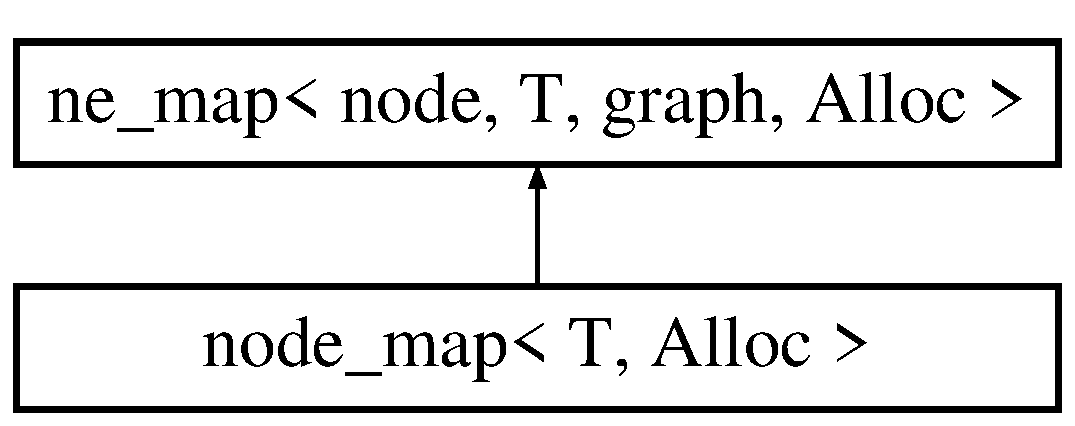
\includegraphics[height=2.000000cm]{classnode__map}
\end{center}
\end{figure}
\subsection*{Public Member Functions}
\begin{DoxyCompactItemize}
\item 
\mbox{\hyperlink{classnode__map_a7a4c767f07f348d31a1004776485d17b}{node\+\_\+map}} ()
\item 
\mbox{\hyperlink{classnode__map_a5bd24349e3a56379592889abbe4c6b09}{node\+\_\+map}} (const \mbox{\hyperlink{classgraph}{graph}} \&g, T t=T())
\end{DoxyCompactItemize}
\subsection*{Additional Inherited Members}


\subsection{Detailed Description}
\subsubsection*{template$<$class T, class Alloc = allocator$<$\+T$>$$>$\newline
class node\+\_\+map$<$ T, Alloc $>$}

A specialized map with nodes as keys. 

A {\ttfamily \mbox{\hyperlink{classnode__map}{node\+\_\+map}}} is a specialized and optimized map implementation with nodes as keys. Using a {\ttfamily \mbox{\hyperlink{classnode__map}{node\+\_\+map}}} is the standard way to attach user defined information to the nodes of a {\ttfamily graph}.

An example of usage\+: 
\begin{DoxyPre}
  graph g;\end{DoxyPre}



\begin{DoxyPre}  node v1 = g.new\_node();
  node v2 = g.new\_node();\end{DoxyPre}



\begin{DoxyPre}  \mbox{\hyperlink{classnode__map}{node\_map}}<string> label(g, "Default Label");\end{DoxyPre}



\begin{DoxyPre}  label[v1] = "v1";
  label[v2] = "v2";\end{DoxyPre}



\begin{DoxyPre}  assert(label[v1] != label[v2]);
\end{DoxyPre}


The nodes used as keys for a {\ttfamily \mbox{\hyperlink{classnode__map}{node\+\_\+map}}} M\+U\+ST be nodes of the same graph. If you want to use nodes from different graphs, use a {\ttfamily map$<$node,T$>$} instead. A graph and a copy of it are considered to be different.

Most of the functionality of {\ttfamily \mbox{\hyperlink{classnode__map}{node\+\_\+map}}} is inherited from \mbox{\hyperlink{classne__map}{ne\+\_\+map}}.

\begin{DoxySeeAlso}{See also}
\mbox{\hyperlink{classedge__map}{edge\+\_\+map}} 
\end{DoxySeeAlso}


\subsection{Constructor \& Destructor Documentation}
\mbox{\Hypertarget{classnode__map_a7a4c767f07f348d31a1004776485d17b}\label{classnode__map_a7a4c767f07f348d31a1004776485d17b}} 
\index{node\+\_\+map@{node\+\_\+map}!node\+\_\+map@{node\+\_\+map}}
\index{node\+\_\+map@{node\+\_\+map}!node\+\_\+map@{node\+\_\+map}}
\subsubsection{\texorpdfstring{node\+\_\+map()}{node\_map()}\hspace{0.1cm}{\footnotesize\ttfamily [1/2]}}
{\footnotesize\ttfamily template$<$class T, class Alloc = allocator$<$\+T$>$$>$ \\
\mbox{\hyperlink{classnode__map}{node\+\_\+map}}$<$ T, Alloc $>$\+::\mbox{\hyperlink{classnode__map}{node\+\_\+map}} (\begin{DoxyParamCaption}{ }\end{DoxyParamCaption})\hspace{0.3cm}{\ttfamily [inline]}}

Constructs an empty {\ttfamily \mbox{\hyperlink{classnode__map}{node\+\_\+map}}} not associated with any {\ttfamily graph}. You may (but need not) call {\ttfamily ne\+\_\+map\+::init(const graph \&, T)} to associate it to a {\ttfamily graph}. \mbox{\Hypertarget{classnode__map_a5bd24349e3a56379592889abbe4c6b09}\label{classnode__map_a5bd24349e3a56379592889abbe4c6b09}} 
\index{node\+\_\+map@{node\+\_\+map}!node\+\_\+map@{node\+\_\+map}}
\index{node\+\_\+map@{node\+\_\+map}!node\+\_\+map@{node\+\_\+map}}
\subsubsection{\texorpdfstring{node\+\_\+map()}{node\_map()}\hspace{0.1cm}{\footnotesize\ttfamily [2/2]}}
{\footnotesize\ttfamily template$<$class T, class Alloc = allocator$<$\+T$>$$>$ \\
\mbox{\hyperlink{classnode__map}{node\+\_\+map}}$<$ T, Alloc $>$\+::\mbox{\hyperlink{classnode__map}{node\+\_\+map}} (\begin{DoxyParamCaption}\item[{const \mbox{\hyperlink{classgraph}{graph}} \&}]{g,  }\item[{T}]{t = {\ttfamily T()} }\end{DoxyParamCaption})\hspace{0.3cm}{\ttfamily [inline]}, {\ttfamily [explicit]}}

Constructs a {\ttfamily \mbox{\hyperlink{classnode__map}{node\+\_\+map}}} associated to the graph {\ttfamily g}. The value associated to each node in {\ttfamily g} is set to {\ttfamily t}. 

The documentation for this class was generated from the following file\+:\begin{DoxyCompactItemize}
\item 
include/\+K\+G\+L/node\+\_\+map.\+h\end{DoxyCompactItemize}

\hypertarget{classp__node}{}\section{p\+\_\+node Class Reference}
\label{classp__node}\index{p\+\_\+node@{p\+\_\+node}}
Inheritance diagram for p\+\_\+node\+:\begin{figure}[H]
\begin{center}
\leavevmode
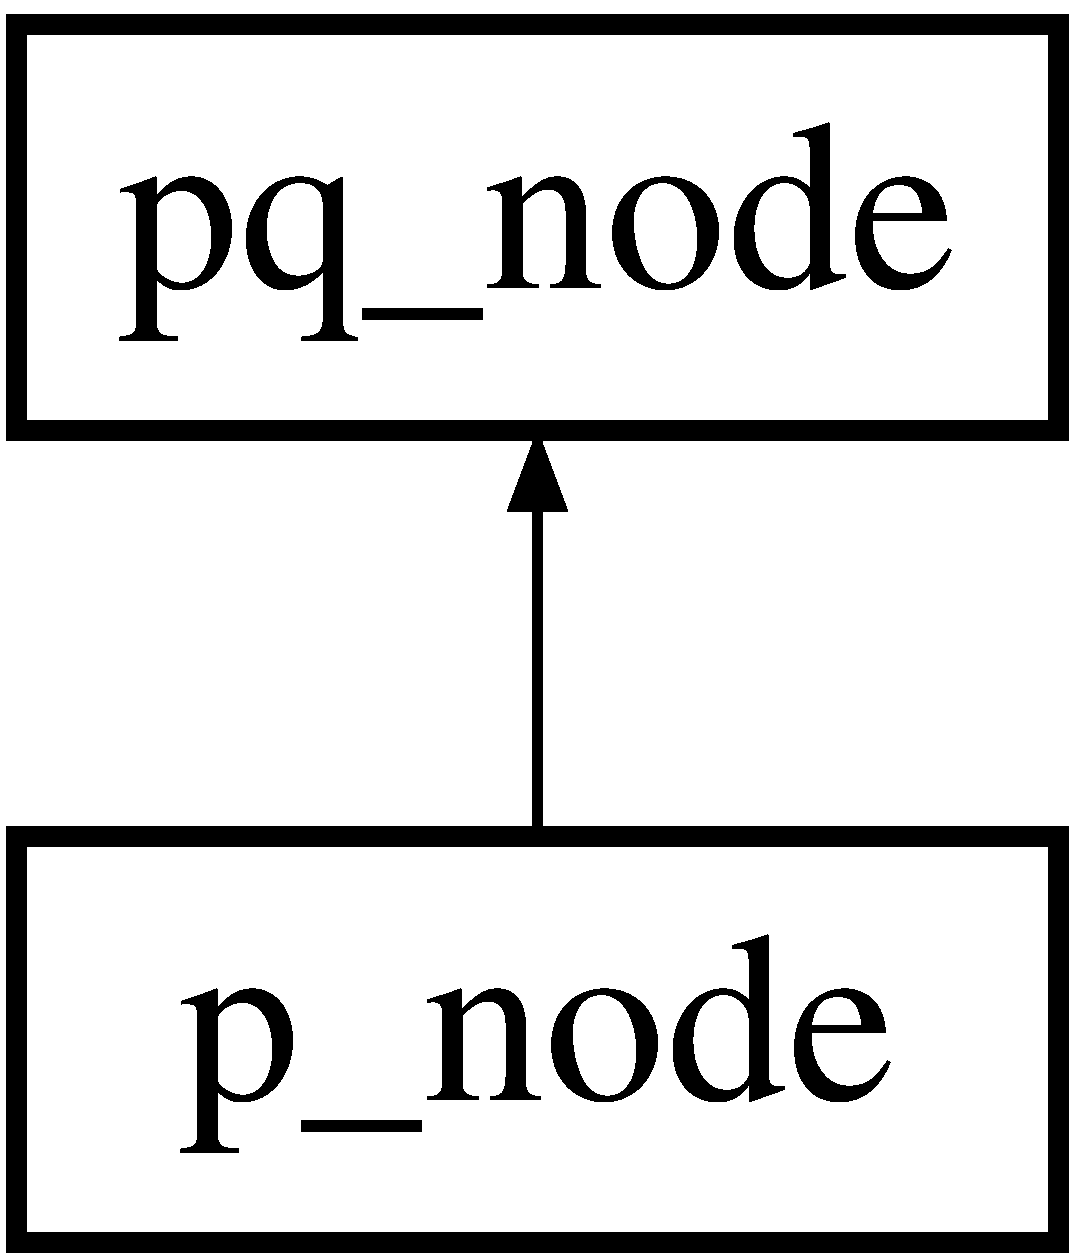
\includegraphics[height=2.000000cm]{classp__node}
\end{center}
\end{figure}
\subsection*{Friends}
\begin{DoxyCompactItemize}
\item 
\mbox{\Hypertarget{classp__node_ab6a02224dbc06343d95919289aec77c8}\label{classp__node_ab6a02224dbc06343d95919289aec77c8}} 
class {\bfseries planarity}
\item 
\mbox{\Hypertarget{classp__node_a0a5be4bb438c891059fae98f607f2a9c}\label{classp__node_a0a5be4bb438c891059fae98f607f2a9c}} 
class {\bfseries pq\+\_\+tree}
\item 
\mbox{\Hypertarget{classp__node_a2e8bee8ed51cc9d2567b69099c4d7cca}\label{classp__node_a2e8bee8ed51cc9d2567b69099c4d7cca}} 
K\+G\+L\+\_\+\+E\+X\+T\+E\+RN friend ostream \& {\bfseries operator$<$$<$} (ostream \&, const \mbox{\hyperlink{classpq__tree}{pq\+\_\+tree}} \&)
\end{DoxyCompactItemize}
\subsection*{Additional Inherited Members}


The documentation for this class was generated from the following files\+:\begin{DoxyCompactItemize}
\item 
include/\+K\+G\+L/pq\+\_\+node.\+h\item 
src/pq\+\_\+node.\+cpp\end{DoxyCompactItemize}

\hypertarget{classpathfinder}{}\section{pathfinder Class Reference}
\label{classpathfinder}\index{pathfinder@{pathfinder}}
\subsection*{Classes}
\begin{DoxyCompactItemize}
\item 
class \mbox{\hyperlink{classpathfinder_1_1const__iterator}{const\+\_\+iterator}}
\end{DoxyCompactItemize}
\subsection*{Public Member Functions}
\begin{DoxyCompactItemize}
\item 
\mbox{\Hypertarget{classpathfinder_ac76b30da32ebf780bf42cdb6da2d2376}\label{classpathfinder_ac76b30da32ebf780bf42cdb6da2d2376}} 
{\bfseries pathfinder} (const \mbox{\hyperlink{classgraph}{graph}} \&G, \mbox{\hyperlink{classedge}{edge}} st, \mbox{\hyperlink{classnode}{node}} s)
\item 
\mbox{\Hypertarget{classpathfinder_a3e595928f8f00bb7b9639f82684f8f05}\label{classpathfinder_a3e595928f8f00bb7b9639f82684f8f05}} 
bool {\bfseries is\+\_\+valid} ()
\item 
\mbox{\Hypertarget{classpathfinder_ab4fffc6da33fb6b1e6badf3a4b3cfed4}\label{classpathfinder_ab4fffc6da33fb6b1e6badf3a4b3cfed4}} 
\mbox{\hyperlink{classpathfinder_1_1const__iterator}{const\+\_\+iterator}} {\bfseries path} (\mbox{\hyperlink{classnode}{node}} n)
\item 
\mbox{\Hypertarget{classpathfinder_a2421f20a6252a46fbc1955322b0f9c55}\label{classpathfinder_a2421f20a6252a46fbc1955322b0f9c55}} 
\mbox{\hyperlink{classpathfinder_1_1const__iterator}{const\+\_\+iterator}} {\bfseries end} ()
\end{DoxyCompactItemize}
\subsection*{Friends}
\begin{DoxyCompactItemize}
\item 
\mbox{\Hypertarget{classpathfinder_ac220ce1c155db1ac44146c12d178056f}\label{classpathfinder_ac220ce1c155db1ac44146c12d178056f}} 
class {\bfseries const\+\_\+iterator}
\end{DoxyCompactItemize}


The documentation for this class was generated from the following files\+:\begin{DoxyCompactItemize}
\item 
include/\+K\+G\+L/st\+\_\+number.\+h\item 
src/st\+\_\+number.\+cpp\end{DoxyCompactItemize}

\hypertarget{classplanar__embedding}{}\section{planar\+\_\+embedding Class Reference}
\label{classplanar__embedding}\index{planar\+\_\+embedding@{planar\+\_\+embedding}}


Ordered adjacency lists as a result of planarity testing.  




{\ttfamily \#include $<$embedding.\+h$>$}

\subsection*{Public Types}
\begin{DoxyCompactItemize}
\item 
\mbox{\Hypertarget{classplanar__embedding_a2f2057ce2f9c23616696042457fd52ff}\label{classplanar__embedding_a2f2057ce2f9c23616696042457fd52ff}} 
typedef \mbox{\hyperlink{classsymlist}{symlist}}$<$ \mbox{\hyperlink{classedge}{edge}} $>$ {\bfseries adj\+\_\+list}
\item 
\mbox{\Hypertarget{classplanar__embedding_a2a2da42b192eb461aad874f0a7e1e430}\label{classplanar__embedding_a2a2da42b192eb461aad874f0a7e1e430}} 
typedef \mbox{\hyperlink{classsymlist}{symlist}}$<$ \mbox{\hyperlink{classedge}{edge}} $>$\+::\mbox{\hyperlink{structsymlist__iterator}{iterator}} {\bfseries iterator}
\end{DoxyCompactItemize}
\subsection*{Public Member Functions}
\begin{DoxyCompactItemize}
\item 
\mbox{\hyperlink{classplanar__embedding_ac3bce79522ec180819470bd0370eda87}{planar\+\_\+embedding}} (const \mbox{\hyperlink{classplanar__embedding}{planar\+\_\+embedding}} \&em)
\item 
virtual \mbox{\hyperlink{classplanar__embedding_ae5605eb5f21346f3f8194dd2db9de117}{$\sim$planar\+\_\+embedding}} ()
\item 
\mbox{\hyperlink{classplanar__embedding}{planar\+\_\+embedding}} \& \mbox{\hyperlink{classplanar__embedding_afb772a5c6a3a03fafa6bbc17a4c42a23}{operator=}} (const \mbox{\hyperlink{classplanar__embedding}{planar\+\_\+embedding}} \&em)
\item 
\mbox{\hyperlink{classsymlist}{adj\+\_\+list}} \& \mbox{\hyperlink{classplanar__embedding_a151a1e7cf6cfbbd0a09c467ec8bc61d1}{adjacency}} (\mbox{\hyperlink{classnode}{node}} n)
\item 
const \mbox{\hyperlink{classsymlist}{adj\+\_\+list}} \& \mbox{\hyperlink{classplanar__embedding_aa52d4454ff761f0130e8739a53efbe83}{adjacency}} (\mbox{\hyperlink{classnode}{node}} n) const
\item 
\mbox{\hyperlink{structsymlist__iterator}{iterator}} \mbox{\hyperlink{classplanar__embedding_ac0b41dd43adb80ed898b597e791230d8}{adj\+\_\+edges\+\_\+begin}} (\mbox{\hyperlink{classnode}{node}} n)
\item 
\mbox{\hyperlink{structsymlist__iterator}{iterator}} \mbox{\hyperlink{classplanar__embedding_a1345ee93995019d81cc78fb2806acc88}{adj\+\_\+edges\+\_\+end}} (\mbox{\hyperlink{classnode}{node}} n)
\item 
\mbox{\hyperlink{classedge}{edge}} \mbox{\hyperlink{classplanar__embedding_a4498733be831e1468044db038452efa4}{cyclic\+\_\+next}} (\mbox{\hyperlink{classnode}{node}} n, \mbox{\hyperlink{classedge}{edge}} e)
\item 
\mbox{\hyperlink{classedge}{edge}} \mbox{\hyperlink{classplanar__embedding_ae4d5e8226c1088c17e15ee6447133383}{cyclic\+\_\+prev}} (\mbox{\hyperlink{classnode}{node}} n, \mbox{\hyperlink{classedge}{edge}} e)
\item 
void \mbox{\hyperlink{classplanar__embedding_ab2870ca51d0df44f8006ab69c3ee74d4}{write\+\_\+st}} (ostream \&os, \mbox{\hyperlink{classst__number}{st\+\_\+number}} \&st)
\item 
list$<$ \mbox{\hyperlink{classedge}{edge}} $>$ \& \mbox{\hyperlink{classplanar__embedding_ab04859be18352bc53a120b0676a499ba}{selfloops}} ()
\item 
const list$<$ \mbox{\hyperlink{classedge}{edge}} $>$ \& \mbox{\hyperlink{classplanar__embedding_a25e47defbdda4552bf1ff98a3e7682e5}{selfloops}} () const
\item 
list$<$ \mbox{\hyperlink{classedge}{edge}} $>$ \& \mbox{\hyperlink{classplanar__embedding_afb50ef8f3b5b2c6690b9d364db21f36f}{multiple\+\_\+edges}} ()
\item 
const list$<$ \mbox{\hyperlink{classedge}{edge}} $>$ \& \mbox{\hyperlink{classplanar__embedding_aebec933f9aac54914ee7439028e37418}{multiple\+\_\+edges}} () const
\item 
bool \mbox{\hyperlink{classplanar__embedding_a6462d40327bf7c4c91523b888bb45cb3}{check}} ()
\end{DoxyCompactItemize}
\subsection*{Friends}
\begin{DoxyCompactItemize}
\item 
\mbox{\Hypertarget{classplanar__embedding_ab6a02224dbc06343d95919289aec77c8}\label{classplanar__embedding_ab6a02224dbc06343d95919289aec77c8}} 
class {\bfseries planarity}
\item 
\mbox{\Hypertarget{classplanar__embedding_a0a5be4bb438c891059fae98f607f2a9c}\label{classplanar__embedding_a0a5be4bb438c891059fae98f607f2a9c}} 
class {\bfseries pq\+\_\+tree}
\item 
\mbox{\Hypertarget{classplanar__embedding_ac972f6f97db38c01e25404f661bc9355}\label{classplanar__embedding_ac972f6f97db38c01e25404f661bc9355}} 
K\+G\+L\+\_\+\+E\+X\+T\+E\+RN friend ostream \& {\bfseries operator$<$$<$} (ostream \&, \mbox{\hyperlink{classplanar__embedding}{planar\+\_\+embedding}} \&)
\end{DoxyCompactItemize}


\subsection{Detailed Description}
Ordered adjacency lists as a result of planarity testing. 

It is known that if a graph is planar the adjacency list of every node can be ordered in such a way that it reflects the order the adjacent edges will have in a planar drawing around the node. Although the tested graph might have been directed the planar embedding one gets will always correspond to the underlying undirected graph, i.\+e. an edge from {\ttfamily n1} to {\ttfamily n2} will occurr in both adjacency lists. 

\subsection{Constructor \& Destructor Documentation}
\mbox{\Hypertarget{classplanar__embedding_ac3bce79522ec180819470bd0370eda87}\label{classplanar__embedding_ac3bce79522ec180819470bd0370eda87}} 
\index{planar\+\_\+embedding@{planar\+\_\+embedding}!planar\+\_\+embedding@{planar\+\_\+embedding}}
\index{planar\+\_\+embedding@{planar\+\_\+embedding}!planar\+\_\+embedding@{planar\+\_\+embedding}}
\subsubsection{\texorpdfstring{planar\+\_\+embedding()}{planar\_embedding()}}
{\footnotesize\ttfamily \+\_\+\+\_\+\+K\+G\+L\+\_\+\+B\+E\+G\+I\+N\+\_\+\+N\+A\+M\+E\+S\+P\+A\+CE planar\+\_\+embedding\+::planar\+\_\+embedding (\begin{DoxyParamCaption}\item[{const \mbox{\hyperlink{classplanar__embedding}{planar\+\_\+embedding}} \&}]{em }\end{DoxyParamCaption})}

Make this object a copy of {\ttfamily em}.


\begin{DoxyParams}{Parameters}
{\em em} & planar embedding \\
\hline
\end{DoxyParams}
\mbox{\Hypertarget{classplanar__embedding_ae5605eb5f21346f3f8194dd2db9de117}\label{classplanar__embedding_ae5605eb5f21346f3f8194dd2db9de117}} 
\index{planar\+\_\+embedding@{planar\+\_\+embedding}!````~planar\+\_\+embedding@{$\sim$planar\+\_\+embedding}}
\index{````~planar\+\_\+embedding@{$\sim$planar\+\_\+embedding}!planar\+\_\+embedding@{planar\+\_\+embedding}}
\subsubsection{\texorpdfstring{$\sim$planar\+\_\+embedding()}{~planar\_embedding()}}
{\footnotesize\ttfamily virtual planar\+\_\+embedding\+::$\sim$planar\+\_\+embedding (\begin{DoxyParamCaption}{ }\end{DoxyParamCaption})\hspace{0.3cm}{\ttfamily [inline]}, {\ttfamily [virtual]}}

Destructor. 

\subsection{Member Function Documentation}
\mbox{\Hypertarget{classplanar__embedding_ac0b41dd43adb80ed898b597e791230d8}\label{classplanar__embedding_ac0b41dd43adb80ed898b597e791230d8}} 
\index{planar\+\_\+embedding@{planar\+\_\+embedding}!adj\+\_\+edges\+\_\+begin@{adj\+\_\+edges\+\_\+begin}}
\index{adj\+\_\+edges\+\_\+begin@{adj\+\_\+edges\+\_\+begin}!planar\+\_\+embedding@{planar\+\_\+embedding}}
\subsubsection{\texorpdfstring{adj\+\_\+edges\+\_\+begin()}{adj\_edges\_begin()}}
{\footnotesize\ttfamily \mbox{\hyperlink{structsymlist__iterator}{iterator}} planar\+\_\+embedding\+::adj\+\_\+edges\+\_\+begin (\begin{DoxyParamCaption}\item[{\mbox{\hyperlink{classnode}{node}}}]{n }\end{DoxyParamCaption})\hspace{0.3cm}{\ttfamily [inline]}}

Start iteration through adjacency list of node {\ttfamily n}.


\begin{DoxyParams}{Parameters}
{\em n} & node\\
\hline
\end{DoxyParams}
\begin{DoxyReturn}{Returns}
start iterator 
\end{DoxyReturn}
\mbox{\Hypertarget{classplanar__embedding_a1345ee93995019d81cc78fb2806acc88}\label{classplanar__embedding_a1345ee93995019d81cc78fb2806acc88}} 
\index{planar\+\_\+embedding@{planar\+\_\+embedding}!adj\+\_\+edges\+\_\+end@{adj\+\_\+edges\+\_\+end}}
\index{adj\+\_\+edges\+\_\+end@{adj\+\_\+edges\+\_\+end}!planar\+\_\+embedding@{planar\+\_\+embedding}}
\subsubsection{\texorpdfstring{adj\+\_\+edges\+\_\+end()}{adj\_edges\_end()}}
{\footnotesize\ttfamily \mbox{\hyperlink{structsymlist__iterator}{iterator}} planar\+\_\+embedding\+::adj\+\_\+edges\+\_\+end (\begin{DoxyParamCaption}\item[{\mbox{\hyperlink{classnode}{node}}}]{n }\end{DoxyParamCaption})\hspace{0.3cm}{\ttfamily [inline]}}

End of iteration through adjacency list of node {\ttfamily n}.


\begin{DoxyParams}{Parameters}
{\em } & \\
\hline
\end{DoxyParams}
\mbox{\Hypertarget{classplanar__embedding_a151a1e7cf6cfbbd0a09c467ec8bc61d1}\label{classplanar__embedding_a151a1e7cf6cfbbd0a09c467ec8bc61d1}} 
\index{planar\+\_\+embedding@{planar\+\_\+embedding}!adjacency@{adjacency}}
\index{adjacency@{adjacency}!planar\+\_\+embedding@{planar\+\_\+embedding}}
\subsubsection{\texorpdfstring{adjacency()}{adjacency()}\hspace{0.1cm}{\footnotesize\ttfamily [1/2]}}
{\footnotesize\ttfamily \mbox{\hyperlink{classsymlist}{adj\+\_\+list}}\& planar\+\_\+embedding\+::adjacency (\begin{DoxyParamCaption}\item[{\mbox{\hyperlink{classnode}{node}}}]{n }\end{DoxyParamCaption})\hspace{0.3cm}{\ttfamily [inline]}}

Returns reference to ordered adjacency list of node {\ttfamily n}.


\begin{DoxyParams}{Parameters}
{\em n} & node\\
\hline
\end{DoxyParams}
\begin{DoxyReturn}{Returns}
ordered adjacency list 
\end{DoxyReturn}
\mbox{\Hypertarget{classplanar__embedding_aa52d4454ff761f0130e8739a53efbe83}\label{classplanar__embedding_aa52d4454ff761f0130e8739a53efbe83}} 
\index{planar\+\_\+embedding@{planar\+\_\+embedding}!adjacency@{adjacency}}
\index{adjacency@{adjacency}!planar\+\_\+embedding@{planar\+\_\+embedding}}
\subsubsection{\texorpdfstring{adjacency()}{adjacency()}\hspace{0.1cm}{\footnotesize\ttfamily [2/2]}}
{\footnotesize\ttfamily const \mbox{\hyperlink{classsymlist}{adj\+\_\+list}}\& planar\+\_\+embedding\+::adjacency (\begin{DoxyParamCaption}\item[{\mbox{\hyperlink{classnode}{node}}}]{n }\end{DoxyParamCaption}) const\hspace{0.3cm}{\ttfamily [inline]}}

Returns reference to ordered adjacency list of node {\ttfamily n}.


\begin{DoxyParams}{Parameters}
{\em n} & node\\
\hline
\end{DoxyParams}
\begin{DoxyReturn}{Returns}
ordered adjacency list 
\end{DoxyReturn}
\mbox{\Hypertarget{classplanar__embedding_a6462d40327bf7c4c91523b888bb45cb3}\label{classplanar__embedding_a6462d40327bf7c4c91523b888bb45cb3}} 
\index{planar\+\_\+embedding@{planar\+\_\+embedding}!check@{check}}
\index{check@{check}!planar\+\_\+embedding@{planar\+\_\+embedding}}
\subsubsection{\texorpdfstring{check()}{check()}}
{\footnotesize\ttfamily bool planar\+\_\+embedding\+::check (\begin{DoxyParamCaption}{ }\end{DoxyParamCaption})}

Used for debugging only. Checks whether this is a correct planar embedding by checking the faces of the graph, i.\+e. at any node starting with an arbitrary adjacent edge and advancing along {\ttfamily cyclic\+\_\+next} the start node must be met through the edge given by {\ttfamily cyclic\+\_\+prev} of the edge we started with.


\begin{DoxyRetVals}{Return values}
{\em true} & iff embedding is correct \\
\hline
\end{DoxyRetVals}
\mbox{\Hypertarget{classplanar__embedding_a4498733be831e1468044db038452efa4}\label{classplanar__embedding_a4498733be831e1468044db038452efa4}} 
\index{planar\+\_\+embedding@{planar\+\_\+embedding}!cyclic\+\_\+next@{cyclic\+\_\+next}}
\index{cyclic\+\_\+next@{cyclic\+\_\+next}!planar\+\_\+embedding@{planar\+\_\+embedding}}
\subsubsection{\texorpdfstring{cyclic\+\_\+next()}{cyclic\_next()}}
{\footnotesize\ttfamily \mbox{\hyperlink{classedge}{edge}} planar\+\_\+embedding\+::cyclic\+\_\+next (\begin{DoxyParamCaption}\item[{\mbox{\hyperlink{classnode}{node}}}]{n,  }\item[{\mbox{\hyperlink{classedge}{edge}}}]{e }\end{DoxyParamCaption})}

Returns the cyclic successor of edge {\ttfamily e} in the adjacency list of node {\ttfamily n}.


\begin{DoxyParams}{Parameters}
{\em n} & node \\
\hline
{\em e} & edge adjacent to {\ttfamily n} \\
\hline
\end{DoxyParams}
\begin{DoxyReturn}{Returns}
edge following {\ttfamily e} in adjacency of {\ttfamily n} 
\end{DoxyReturn}
\mbox{\Hypertarget{classplanar__embedding_ae4d5e8226c1088c17e15ee6447133383}\label{classplanar__embedding_ae4d5e8226c1088c17e15ee6447133383}} 
\index{planar\+\_\+embedding@{planar\+\_\+embedding}!cyclic\+\_\+prev@{cyclic\+\_\+prev}}
\index{cyclic\+\_\+prev@{cyclic\+\_\+prev}!planar\+\_\+embedding@{planar\+\_\+embedding}}
\subsubsection{\texorpdfstring{cyclic\+\_\+prev()}{cyclic\_prev()}}
{\footnotesize\ttfamily \mbox{\hyperlink{classedge}{edge}} planar\+\_\+embedding\+::cyclic\+\_\+prev (\begin{DoxyParamCaption}\item[{\mbox{\hyperlink{classnode}{node}}}]{n,  }\item[{\mbox{\hyperlink{classedge}{edge}}}]{e }\end{DoxyParamCaption})}

Returns the cyclic predecessor of edge {\ttfamily e} in the adjacency list of node {\ttfamily n}.


\begin{DoxyParams}{Parameters}
{\em n} & node \\
\hline
{\em e} & edge adjacent to {\ttfamily n} \\
\hline
\end{DoxyParams}
\begin{DoxyReturn}{Returns}
edge preceding {\ttfamily e} in adjacency of {\ttfamily n} 
\end{DoxyReturn}
\mbox{\Hypertarget{classplanar__embedding_afb50ef8f3b5b2c6690b9d364db21f36f}\label{classplanar__embedding_afb50ef8f3b5b2c6690b9d364db21f36f}} 
\index{planar\+\_\+embedding@{planar\+\_\+embedding}!multiple\+\_\+edges@{multiple\+\_\+edges}}
\index{multiple\+\_\+edges@{multiple\+\_\+edges}!planar\+\_\+embedding@{planar\+\_\+embedding}}
\subsubsection{\texorpdfstring{multiple\+\_\+edges()}{multiple\_edges()}\hspace{0.1cm}{\footnotesize\ttfamily [1/2]}}
{\footnotesize\ttfamily list$<$\mbox{\hyperlink{classedge}{edge}}$>$\& planar\+\_\+embedding\+::multiple\+\_\+edges (\begin{DoxyParamCaption}{ }\end{DoxyParamCaption})\hspace{0.3cm}{\ttfamily [inline]}}

Returns list of multiple edges contained in the graph. These are edges for which there is already another edge connecting the same endpoints is contained in the adjacency lists. Please note that the notion \char`\"{}connecting\char`\"{} is meant in an undirected sense. These edges will not occur it the adjacency lists.


\begin{DoxyRetVals}{Return values}
{\em list} & of multiple edges \\
\hline
\end{DoxyRetVals}
\mbox{\Hypertarget{classplanar__embedding_aebec933f9aac54914ee7439028e37418}\label{classplanar__embedding_aebec933f9aac54914ee7439028e37418}} 
\index{planar\+\_\+embedding@{planar\+\_\+embedding}!multiple\+\_\+edges@{multiple\+\_\+edges}}
\index{multiple\+\_\+edges@{multiple\+\_\+edges}!planar\+\_\+embedding@{planar\+\_\+embedding}}
\subsubsection{\texorpdfstring{multiple\+\_\+edges()}{multiple\_edges()}\hspace{0.1cm}{\footnotesize\ttfamily [2/2]}}
{\footnotesize\ttfamily const list$<$\mbox{\hyperlink{classedge}{edge}}$>$\& planar\+\_\+embedding\+::multiple\+\_\+edges (\begin{DoxyParamCaption}{ }\end{DoxyParamCaption}) const\hspace{0.3cm}{\ttfamily [inline]}}

Returns list of multiple edges contained in the graph. These are edges for which there is already another edge connecting the same endpoints is contained in the adjacency lists. Please note that the notion \char`\"{}connecting\char`\"{} is meant in an undirected sense. These edges will not occur it the adjacency lists.


\begin{DoxyRetVals}{Return values}
{\em list} & of multiple edges \\
\hline
\end{DoxyRetVals}
\mbox{\Hypertarget{classplanar__embedding_afb772a5c6a3a03fafa6bbc17a4c42a23}\label{classplanar__embedding_afb772a5c6a3a03fafa6bbc17a4c42a23}} 
\index{planar\+\_\+embedding@{planar\+\_\+embedding}!operator=@{operator=}}
\index{operator=@{operator=}!planar\+\_\+embedding@{planar\+\_\+embedding}}
\subsubsection{\texorpdfstring{operator=()}{operator=()}}
{\footnotesize\ttfamily \mbox{\hyperlink{classplanar__embedding}{planar\+\_\+embedding}} \& planar\+\_\+embedding\+::operator= (\begin{DoxyParamCaption}\item[{const \mbox{\hyperlink{classplanar__embedding}{planar\+\_\+embedding}} \&}]{em }\end{DoxyParamCaption})}

Assigns {\ttfamily em} to this object. All former information in this object will be deleted.


\begin{DoxyParams}{Parameters}
{\em em} & \\
\hline
\end{DoxyParams}
\begin{DoxyReturn}{Returns}
reference to this object 
\end{DoxyReturn}
\mbox{\Hypertarget{classplanar__embedding_ab04859be18352bc53a120b0676a499ba}\label{classplanar__embedding_ab04859be18352bc53a120b0676a499ba}} 
\index{planar\+\_\+embedding@{planar\+\_\+embedding}!selfloops@{selfloops}}
\index{selfloops@{selfloops}!planar\+\_\+embedding@{planar\+\_\+embedding}}
\subsubsection{\texorpdfstring{selfloops()}{selfloops()}\hspace{0.1cm}{\footnotesize\ttfamily [1/2]}}
{\footnotesize\ttfamily list$<$\mbox{\hyperlink{classedge}{edge}}$>$\& planar\+\_\+embedding\+::selfloops (\begin{DoxyParamCaption}{ }\end{DoxyParamCaption})\hspace{0.3cm}{\ttfamily [inline]}}

Returns list of selfloops contained in the graph. These will not occur in the adjacency lists.


\begin{DoxyRetVals}{Return values}
{\em list} & of selfloops \\
\hline
\end{DoxyRetVals}
\mbox{\Hypertarget{classplanar__embedding_a25e47defbdda4552bf1ff98a3e7682e5}\label{classplanar__embedding_a25e47defbdda4552bf1ff98a3e7682e5}} 
\index{planar\+\_\+embedding@{planar\+\_\+embedding}!selfloops@{selfloops}}
\index{selfloops@{selfloops}!planar\+\_\+embedding@{planar\+\_\+embedding}}
\subsubsection{\texorpdfstring{selfloops()}{selfloops()}\hspace{0.1cm}{\footnotesize\ttfamily [2/2]}}
{\footnotesize\ttfamily const list$<$\mbox{\hyperlink{classedge}{edge}}$>$\& planar\+\_\+embedding\+::selfloops (\begin{DoxyParamCaption}{ }\end{DoxyParamCaption}) const\hspace{0.3cm}{\ttfamily [inline]}}

Returns list of selfloops contained in the graph. These will not occur in the adjacency lists.


\begin{DoxyRetVals}{Return values}
{\em list} & of selfloops \\
\hline
\end{DoxyRetVals}
\mbox{\Hypertarget{classplanar__embedding_ab2870ca51d0df44f8006ab69c3ee74d4}\label{classplanar__embedding_ab2870ca51d0df44f8006ab69c3ee74d4}} 
\index{planar\+\_\+embedding@{planar\+\_\+embedding}!write\+\_\+st@{write\+\_\+st}}
\index{write\+\_\+st@{write\+\_\+st}!planar\+\_\+embedding@{planar\+\_\+embedding}}
\subsubsection{\texorpdfstring{write\+\_\+st()}{write\_st()}}
{\footnotesize\ttfamily void planar\+\_\+embedding\+::write\+\_\+st (\begin{DoxyParamCaption}\item[{ostream \&}]{os,  }\item[{\mbox{\hyperlink{classst__number}{st\+\_\+number}} \&}]{st }\end{DoxyParamCaption})}

Writes embedding with st-\/numbers as given by {\ttfamily st} to {\ttfamily os}.


\begin{DoxyParams}{Parameters}
{\em os} & output stream\\
\hline
{\em st} & st-\/numbers \\
\hline
\end{DoxyParams}


The documentation for this class was generated from the following files\+:\begin{DoxyCompactItemize}
\item 
include/\+K\+G\+L/embedding.\+h\item 
src/embedding.\+cpp\end{DoxyCompactItemize}

\hypertarget{classplanarity}{}\section{planarity Class Reference}
\label{classplanarity}\index{planarity@{planarity}}


Tests if a graph can be drawn on a plane without any edge crossings.  




{\ttfamily \#include $<$planarity.\+h$>$}

Inheritance diagram for planarity\+:\begin{figure}[H]
\begin{center}
\leavevmode
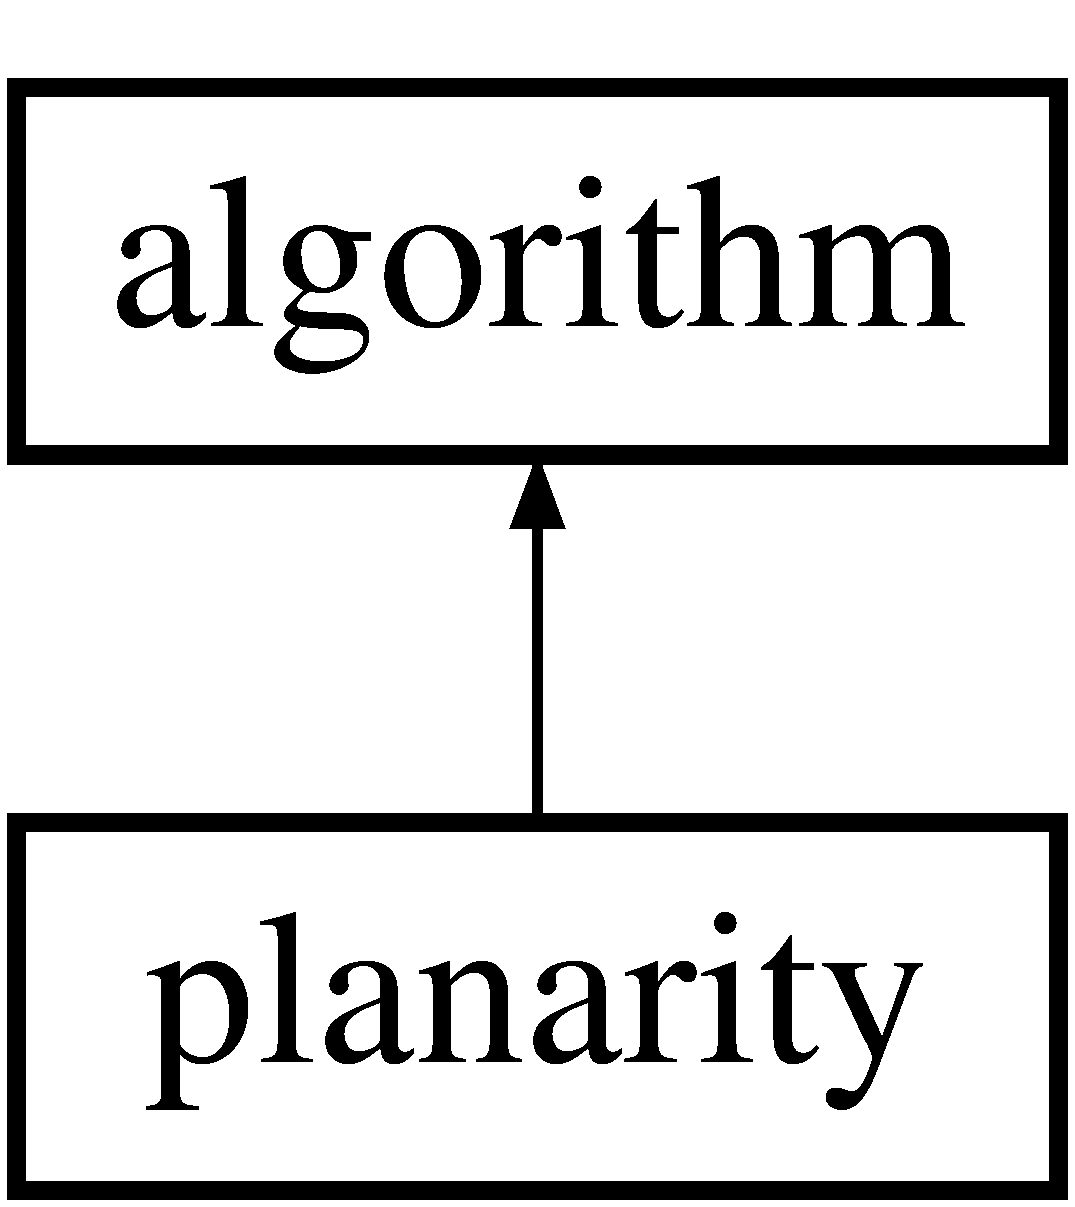
\includegraphics[height=2.000000cm]{classplanarity}
\end{center}
\end{figure}
\subsection*{Public Member Functions}
\begin{DoxyCompactItemize}
\item 
\mbox{\hyperlink{classplanarity_ab0377cf75279277a848f7e2eed507d00}{planarity}} ()
\begin{DoxyCompactList}\small\item\em Creates an object of the planarity test algorithm. \end{DoxyCompactList}\item 
\mbox{\Hypertarget{classplanarity_a3e0c0f1a724191042947dfecc640bf05}\label{classplanarity_a3e0c0f1a724191042947dfecc640bf05}} 
\mbox{\hyperlink{classplanarity_a3e0c0f1a724191042947dfecc640bf05}{$\sim$planarity}} ()
\begin{DoxyCompactList}\small\item\em Destructor. \end{DoxyCompactList}\item 
int \mbox{\hyperlink{classplanarity_ae06c471d957a116aad14e338c341f8b1}{check}} (\mbox{\hyperlink{classgraph}{graph}} \&G)
\begin{DoxyCompactList}\small\item\em Checks whether planarity test can be applied to {\ttfamily G}. \end{DoxyCompactList}\item 
int \mbox{\hyperlink{classplanarity_a93232e765c08dd2a4c00d192bb48b5fc}{run}} (\mbox{\hyperlink{classgraph}{graph}} \&G)
\begin{DoxyCompactList}\small\item\em Runs planarity test on {\ttfamily G}. \end{DoxyCompactList}\item 
void \mbox{\hyperlink{classplanarity_aca500e3d46a99c6231aff86afa2a71b1}{reset}} ()
\begin{DoxyCompactList}\small\item\em Resets algorithm object, such that it can be applied to another graph. \end{DoxyCompactList}\item 
void \mbox{\hyperlink{classplanarity_a1679e285a7135b48b572764f5e8e773d}{calc\+\_\+embedding}} (bool p)
\begin{DoxyCompactList}\small\item\em If {\ttfamily p} is true a planar embedding will be calculated in the next run. \end{DoxyCompactList}\item 
bool \mbox{\hyperlink{classplanarity_aea94b0de2deb46ef774179dd3572bf2d}{calc\+\_\+embedding}} () const
\begin{DoxyCompactList}\small\item\em Returns true if a planar embedding will be calculated in the next run. \end{DoxyCompactList}\item 
void \mbox{\hyperlink{classplanarity_a7b8e8e5414a4eedb0f99253d3b62ffa3}{calc\+\_\+obstruction}} (bool p)
\begin{DoxyCompactList}\small\item\em If {\ttfamily p} is true the obstructions to planarity will be calculated in the next run. \end{DoxyCompactList}\item 
bool \mbox{\hyperlink{classplanarity_a0c520ff8f91336a2dc644f9e4ed8bb2e}{calc\+\_\+obstruction}} () const
\begin{DoxyCompactList}\small\item\em Returns true if the obstructions to planarity will be calculated in the next run. \end{DoxyCompactList}\item 
void \mbox{\hyperlink{classplanarity_af67236533dce559d2670eae581750f54}{make\+\_\+biconnected}} (bool p)
\begin{DoxyCompactList}\small\item\em Determines the strategy used to test a graph which is not biconnected. \end{DoxyCompactList}\item 
bool \mbox{\hyperlink{classplanarity_a822d67100814e1887494e7213e6f0531}{make\+\_\+biconnected}} () const
\begin{DoxyCompactList}\small\item\em Returns strategy for testing graphs, which are not biconnected. \end{DoxyCompactList}\item 
bool \mbox{\hyperlink{classplanarity_af60c3d06cffa7ce3a470797fd758be5f}{is\+\_\+planar}} () const
\begin{DoxyCompactList}\small\item\em Result of last test. \end{DoxyCompactList}\item 
\mbox{\hyperlink{classplanar__embedding}{planar\+\_\+embedding}} \& \mbox{\hyperlink{classplanarity_a9ab79a340e361c3300cc08e82edd4e12}{get\+\_\+embedding}} ()
\begin{DoxyCompactList}\small\item\em If graph in last \mbox{\hyperlink{classplanarity_a93232e765c08dd2a4c00d192bb48b5fc}{run}} was planar a planar embedding is calculated during the reductions. This function gives access to it. \end{DoxyCompactList}\item 
list$<$ \mbox{\hyperlink{classedge}{edge}} $>$ \& \mbox{\hyperlink{classplanarity_ac9021696934cc24afbc36aa307b2919b}{get\+\_\+obstruction\+\_\+edges}} ()
\begin{DoxyCompactList}\small\item\em Returns the edges of a subgraph homeomorphic to either K3,3 or K5 if graph in last run was not planar. \end{DoxyCompactList}\item 
list$<$ \mbox{\hyperlink{classnode}{node}} $>$ \& \mbox{\hyperlink{classplanarity_ac1bee50e38d398f3868a3308164caa31}{get\+\_\+obstruction\+\_\+nodes}} ()
\begin{DoxyCompactList}\small\item\em Returns the nodes of a subgraph homeomorphic to either K3,3 or K5 if graph in last run was not planar. \end{DoxyCompactList}\end{DoxyCompactItemize}
\subsection*{Additional Inherited Members}


\subsection{Detailed Description}
Tests if a graph can be drawn on a plane without any edge crossings. 

\begin{DoxyParagraph}{Date}
2019/05/07 18\+:17\+:08 
\end{DoxyParagraph}
\begin{DoxyParagraph}{Revision}
1.\+22 
\end{DoxyParagraph}


This class implements the Lempel-\/\+Even-\/\+Cederbaum planarity test using P\+Q-\/trees. In case the graph is planar a planar embedding is obtained, i.\+e. for each node in the graph an ordered adjacency list is calculated, such that there exists a planar drawing in which all adjacent edges around a node apply to this order.

If the graph is not planar Kuratowski\textquotesingle{}s famous theorem states that it must contain a subgraph hoemeomorphic to either K5 (the complete graph with five nodes) or K3,3 (the complete bipartite graph with three nodes each side). In this case the nodes and edges of the tested graph that form either of these two are calculated.

In case the graph is planar and has $N$ nodes the algorithm needs $\mathcal{O}(N)$ time for the test (including the planar embedding). In case the graph isn\textquotesingle{}t planar it needs at most $\mathcal{O}(E)$ time if $E$ is the number of edges for both the test and the detection of K5 or K3,3. 

\subsection{Constructor \& Destructor Documentation}
\mbox{\Hypertarget{classplanarity_ab0377cf75279277a848f7e2eed507d00}\label{classplanarity_ab0377cf75279277a848f7e2eed507d00}} 
\index{planarity@{planarity}!planarity@{planarity}}
\index{planarity@{planarity}!planarity@{planarity}}
\subsubsection{\texorpdfstring{planarity()}{planarity()}}
{\footnotesize\ttfamily \+\_\+\+\_\+\+K\+G\+L\+\_\+\+B\+E\+G\+I\+N\+\_\+\+N\+A\+M\+E\+S\+P\+A\+CE planarity\+::planarity (\begin{DoxyParamCaption}{ }\end{DoxyParamCaption})}



Creates an object of the planarity test algorithm. 

\begin{DoxySeeAlso}{See also}
\mbox{\hyperlink{classalgorithm}{algorithm}} 
\end{DoxySeeAlso}


\subsection{Member Function Documentation}
\mbox{\Hypertarget{classplanarity_a1679e285a7135b48b572764f5e8e773d}\label{classplanarity_a1679e285a7135b48b572764f5e8e773d}} 
\index{planarity@{planarity}!calc\+\_\+embedding@{calc\+\_\+embedding}}
\index{calc\+\_\+embedding@{calc\+\_\+embedding}!planarity@{planarity}}
\subsubsection{\texorpdfstring{calc\+\_\+embedding()}{calc\_embedding()}\hspace{0.1cm}{\footnotesize\ttfamily [1/2]}}
{\footnotesize\ttfamily void planarity\+::calc\+\_\+embedding (\begin{DoxyParamCaption}\item[{bool}]{p }\end{DoxyParamCaption})\hspace{0.3cm}{\ttfamily [inline]}}



If {\ttfamily p} is true a planar embedding will be calculated in the next run. 


\begin{DoxyParams}{Parameters}
{\em p} & {\ttfamily true} iff embedding should be calculated\\
\hline
\end{DoxyParams}
\begin{DoxySeeAlso}{See also}
\mbox{\hyperlink{classplanarity_a9ab79a340e361c3300cc08e82edd4e12}{get\+\_\+embedding}} 

\mbox{\hyperlink{classplanar__embedding}{planar\+\_\+embedding}} 
\end{DoxySeeAlso}
\mbox{\Hypertarget{classplanarity_aea94b0de2deb46ef774179dd3572bf2d}\label{classplanarity_aea94b0de2deb46ef774179dd3572bf2d}} 
\index{planarity@{planarity}!calc\+\_\+embedding@{calc\+\_\+embedding}}
\index{calc\+\_\+embedding@{calc\+\_\+embedding}!planarity@{planarity}}
\subsubsection{\texorpdfstring{calc\+\_\+embedding()}{calc\_embedding()}\hspace{0.1cm}{\footnotesize\ttfamily [2/2]}}
{\footnotesize\ttfamily bool planarity\+::calc\+\_\+embedding (\begin{DoxyParamCaption}{ }\end{DoxyParamCaption}) const\hspace{0.3cm}{\ttfamily [inline]}}



Returns true if a planar embedding will be calculated in the next run. 


\begin{DoxyRetVals}{Return values}
{\em true} & iff embedding will be calculated\\
\hline
\end{DoxyRetVals}
\begin{DoxySeeAlso}{See also}
\mbox{\hyperlink{classplanarity_a9ab79a340e361c3300cc08e82edd4e12}{get\+\_\+embedding}} 

\mbox{\hyperlink{classplanar__embedding}{planar\+\_\+embedding}} 
\end{DoxySeeAlso}
\mbox{\Hypertarget{classplanarity_a7b8e8e5414a4eedb0f99253d3b62ffa3}\label{classplanarity_a7b8e8e5414a4eedb0f99253d3b62ffa3}} 
\index{planarity@{planarity}!calc\+\_\+obstruction@{calc\+\_\+obstruction}}
\index{calc\+\_\+obstruction@{calc\+\_\+obstruction}!planarity@{planarity}}
\subsubsection{\texorpdfstring{calc\+\_\+obstruction()}{calc\_obstruction()}\hspace{0.1cm}{\footnotesize\ttfamily [1/2]}}
{\footnotesize\ttfamily void planarity\+::calc\+\_\+obstruction (\begin{DoxyParamCaption}\item[{bool}]{p }\end{DoxyParamCaption})\hspace{0.3cm}{\ttfamily [inline]}}



If {\ttfamily p} is true the obstructions to planarity will be calculated in the next run. 

This implies the calculation of an embedding.


\begin{DoxyParams}{Parameters}
{\em p} & {\ttfamily true} iff obstructions to planarity should be calculated\\
\hline
\end{DoxyParams}
\begin{DoxySeeAlso}{See also}
\mbox{\hyperlink{classplanarity_ac9021696934cc24afbc36aa307b2919b}{get\+\_\+obstruction\+\_\+edges}} 

\mbox{\hyperlink{classplanarity_ac1bee50e38d398f3868a3308164caa31}{get\+\_\+obstruction\+\_\+nodes}} 
\end{DoxySeeAlso}
\mbox{\Hypertarget{classplanarity_a0c520ff8f91336a2dc644f9e4ed8bb2e}\label{classplanarity_a0c520ff8f91336a2dc644f9e4ed8bb2e}} 
\index{planarity@{planarity}!calc\+\_\+obstruction@{calc\+\_\+obstruction}}
\index{calc\+\_\+obstruction@{calc\+\_\+obstruction}!planarity@{planarity}}
\subsubsection{\texorpdfstring{calc\+\_\+obstruction()}{calc\_obstruction()}\hspace{0.1cm}{\footnotesize\ttfamily [2/2]}}
{\footnotesize\ttfamily bool planarity\+::calc\+\_\+obstruction (\begin{DoxyParamCaption}{ }\end{DoxyParamCaption}) const\hspace{0.3cm}{\ttfamily [inline]}}



Returns true if the obstructions to planarity will be calculated in the next run. 


\begin{DoxyRetVals}{Return values}
{\em true} & iff obstructions to planarity will be calculated\\
\hline
\end{DoxyRetVals}
\begin{DoxySeeAlso}{See also}
\mbox{\hyperlink{classplanarity_ac9021696934cc24afbc36aa307b2919b}{get\+\_\+obstruction\+\_\+edges}} 

\mbox{\hyperlink{classplanarity_ac1bee50e38d398f3868a3308164caa31}{get\+\_\+obstruction\+\_\+nodes}} 
\end{DoxySeeAlso}
\mbox{\Hypertarget{classplanarity_ae06c471d957a116aad14e338c341f8b1}\label{classplanarity_ae06c471d957a116aad14e338c341f8b1}} 
\index{planarity@{planarity}!check@{check}}
\index{check@{check}!planarity@{planarity}}
\subsubsection{\texorpdfstring{check()}{check()}}
{\footnotesize\ttfamily int planarity\+::check (\begin{DoxyParamCaption}\item[{\mbox{\hyperlink{classgraph}{graph}} \&}]{G }\end{DoxyParamCaption})\hspace{0.3cm}{\ttfamily [virtual]}}



Checks whether planarity test can be applied to {\ttfamily G}. 

This should return always {\ttfamily K\+G\+L\+\_\+\+OK}. There aren\textquotesingle{}t any restrictions on {\ttfamily G}, even multiple edges and selfloops are tolerated.

\begin{DoxyNote}{Note}
Selfloops and multiple edges will not be added to the planar embedding. \mbox{\hyperlink{classplanar__embedding_ab04859be18352bc53a120b0676a499ba}{planar\+\_\+embedding\+::selfloops}} and \mbox{\hyperlink{classplanar__embedding_afb50ef8f3b5b2c6690b9d364db21f36f}{planar\+\_\+embedding\+::multiple\+\_\+edges}} can be used to get these.
\end{DoxyNote}

\begin{DoxyParams}{Parameters}
{\em G} & arbitrary graph\\
\hline
\end{DoxyParams}

\begin{DoxyRetVals}{Return values}
{\em K\+G\+L\+\_\+\+OK} & if planarity test can be applied \\
\hline
{\em K\+G\+L\+\_\+\+E\+R\+R\+OR} & if not\\
\hline
\end{DoxyRetVals}
\begin{DoxySeeAlso}{See also}
\mbox{\hyperlink{classalgorithm_a76361fb03ad1cf643affc51821e43bed}{algorithm\+::check}} 
\end{DoxySeeAlso}


Implements \mbox{\hyperlink{classalgorithm_a76361fb03ad1cf643affc51821e43bed}{algorithm}}.

\mbox{\Hypertarget{classplanarity_a9ab79a340e361c3300cc08e82edd4e12}\label{classplanarity_a9ab79a340e361c3300cc08e82edd4e12}} 
\index{planarity@{planarity}!get\+\_\+embedding@{get\+\_\+embedding}}
\index{get\+\_\+embedding@{get\+\_\+embedding}!planarity@{planarity}}
\subsubsection{\texorpdfstring{get\+\_\+embedding()}{get\_embedding()}}
{\footnotesize\ttfamily \mbox{\hyperlink{classplanar__embedding}{planar\+\_\+embedding}}\& planarity\+::get\+\_\+embedding (\begin{DoxyParamCaption}{ }\end{DoxyParamCaption})\hspace{0.3cm}{\ttfamily [inline]}}



If graph in last \mbox{\hyperlink{classplanarity_a93232e765c08dd2a4c00d192bb48b5fc}{run}} was planar a planar embedding is calculated during the reductions. This function gives access to it. 

\begin{DoxyReturn}{Returns}
planar embedding of graph in last run
\end{DoxyReturn}
\begin{DoxySeeAlso}{See also}
\mbox{\hyperlink{classplanarity_a1679e285a7135b48b572764f5e8e773d}{calc\+\_\+embedding}} 
\end{DoxySeeAlso}
\mbox{\Hypertarget{classplanarity_ac9021696934cc24afbc36aa307b2919b}\label{classplanarity_ac9021696934cc24afbc36aa307b2919b}} 
\index{planarity@{planarity}!get\+\_\+obstruction\+\_\+edges@{get\+\_\+obstruction\+\_\+edges}}
\index{get\+\_\+obstruction\+\_\+edges@{get\+\_\+obstruction\+\_\+edges}!planarity@{planarity}}
\subsubsection{\texorpdfstring{get\+\_\+obstruction\+\_\+edges()}{get\_obstruction\_edges()}}
{\footnotesize\ttfamily list$<$\mbox{\hyperlink{classedge}{edge}}$>$\& planarity\+::get\+\_\+obstruction\+\_\+edges (\begin{DoxyParamCaption}{ }\end{DoxyParamCaption})\hspace{0.3cm}{\ttfamily [inline]}}



Returns the edges of a subgraph homeomorphic to either K3,3 or K5 if graph in last run was not planar. 

\begin{DoxyReturn}{Returns}
edges of subgraph homeomorphic to either K3,3 or K5
\end{DoxyReturn}
\begin{DoxySeeAlso}{See also}
\mbox{\hyperlink{classplanarity_ac1bee50e38d398f3868a3308164caa31}{get\+\_\+obstruction\+\_\+nodes}} 

\mbox{\hyperlink{classplanarity_a7b8e8e5414a4eedb0f99253d3b62ffa3}{calc\+\_\+obstruction}} 
\end{DoxySeeAlso}
\mbox{\Hypertarget{classplanarity_ac1bee50e38d398f3868a3308164caa31}\label{classplanarity_ac1bee50e38d398f3868a3308164caa31}} 
\index{planarity@{planarity}!get\+\_\+obstruction\+\_\+nodes@{get\+\_\+obstruction\+\_\+nodes}}
\index{get\+\_\+obstruction\+\_\+nodes@{get\+\_\+obstruction\+\_\+nodes}!planarity@{planarity}}
\subsubsection{\texorpdfstring{get\+\_\+obstruction\+\_\+nodes()}{get\_obstruction\_nodes()}}
{\footnotesize\ttfamily list$<$\mbox{\hyperlink{classnode}{node}}$>$\& planarity\+::get\+\_\+obstruction\+\_\+nodes (\begin{DoxyParamCaption}{ }\end{DoxyParamCaption})\hspace{0.3cm}{\ttfamily [inline]}}



Returns the nodes of a subgraph homeomorphic to either K3,3 or K5 if graph in last run was not planar. 

\begin{DoxyReturn}{Returns}
nodes of subgraph homeomorphic to either K3,3 or K5
\end{DoxyReturn}
\begin{DoxySeeAlso}{See also}
\mbox{\hyperlink{classplanarity_ac9021696934cc24afbc36aa307b2919b}{get\+\_\+obstruction\+\_\+edges}} 

\mbox{\hyperlink{classplanarity_a7b8e8e5414a4eedb0f99253d3b62ffa3}{calc\+\_\+obstruction}} 
\end{DoxySeeAlso}
\mbox{\Hypertarget{classplanarity_af60c3d06cffa7ce3a470797fd758be5f}\label{classplanarity_af60c3d06cffa7ce3a470797fd758be5f}} 
\index{planarity@{planarity}!is\+\_\+planar@{is\+\_\+planar}}
\index{is\+\_\+planar@{is\+\_\+planar}!planarity@{planarity}}
\subsubsection{\texorpdfstring{is\+\_\+planar()}{is\_planar()}}
{\footnotesize\ttfamily bool planarity\+::is\+\_\+planar (\begin{DoxyParamCaption}{ }\end{DoxyParamCaption}) const\hspace{0.3cm}{\ttfamily [inline]}}



Result of last test. 


\begin{DoxyRetVals}{Return values}
{\em true} & iff graph in last run was planar. \\
\hline
\end{DoxyRetVals}
\mbox{\Hypertarget{classplanarity_af67236533dce559d2670eae581750f54}\label{classplanarity_af67236533dce559d2670eae581750f54}} 
\index{planarity@{planarity}!make\+\_\+biconnected@{make\+\_\+biconnected}}
\index{make\+\_\+biconnected@{make\+\_\+biconnected}!planarity@{planarity}}
\subsubsection{\texorpdfstring{make\+\_\+biconnected()}{make\_biconnected()}\hspace{0.1cm}{\footnotesize\ttfamily [1/2]}}
{\footnotesize\ttfamily void planarity\+::make\+\_\+biconnected (\begin{DoxyParamCaption}\item[{bool}]{p }\end{DoxyParamCaption})\hspace{0.3cm}{\ttfamily [inline]}}



Determines the strategy used to test a graph which is not biconnected. 

If this is enabled the graph will be made biconnected by adding some new edges. This is usually faster than testing the biconnected components one by one, which is done if this option is disabled. By default this is enabled.

\begin{DoxyNote}{Note}
This is not fully tested, i.\+e. at the moment this feature should be used only for the test without embedding or kuratowski graphs.
\end{DoxyNote}

\begin{DoxyParams}{Parameters}
{\em p} & true iff graph should be made biconnected\\
\hline
\end{DoxyParams}
\begin{DoxySeeAlso}{See also}
\mbox{\hyperlink{classbiconnectivity_a774fd08203a6d164605afc4cdc8b9201}{biconnectivity\+::make\+\_\+biconnected}} 
\end{DoxySeeAlso}
\mbox{\Hypertarget{classplanarity_a822d67100814e1887494e7213e6f0531}\label{classplanarity_a822d67100814e1887494e7213e6f0531}} 
\index{planarity@{planarity}!make\+\_\+biconnected@{make\+\_\+biconnected}}
\index{make\+\_\+biconnected@{make\+\_\+biconnected}!planarity@{planarity}}
\subsubsection{\texorpdfstring{make\+\_\+biconnected()}{make\_biconnected()}\hspace{0.1cm}{\footnotesize\ttfamily [2/2]}}
{\footnotesize\ttfamily bool planarity\+::make\+\_\+biconnected (\begin{DoxyParamCaption}{ }\end{DoxyParamCaption}) const\hspace{0.3cm}{\ttfamily [inline]}}



Returns strategy for testing graphs, which are not biconnected. 


\begin{DoxyRetVals}{Return values}
{\em true} & iff graph will be made biconnected before test\\
\hline
\end{DoxyRetVals}
\begin{DoxySeeAlso}{See also}
\mbox{\hyperlink{classbiconnectivity_a774fd08203a6d164605afc4cdc8b9201}{biconnectivity\+::make\+\_\+biconnected}} 
\end{DoxySeeAlso}
\mbox{\Hypertarget{classplanarity_aca500e3d46a99c6231aff86afa2a71b1}\label{classplanarity_aca500e3d46a99c6231aff86afa2a71b1}} 
\index{planarity@{planarity}!reset@{reset}}
\index{reset@{reset}!planarity@{planarity}}
\subsubsection{\texorpdfstring{reset()}{reset()}}
{\footnotesize\ttfamily void planarity\+::reset (\begin{DoxyParamCaption}{ }\end{DoxyParamCaption})\hspace{0.3cm}{\ttfamily [virtual]}}



Resets algorithm object, such that it can be applied to another graph. 

\begin{DoxySeeAlso}{See also}
\mbox{\hyperlink{classalgorithm_a21aba63d066ae7897de6ca7d8425c408}{algorithm\+::reset}} 
\end{DoxySeeAlso}


Implements \mbox{\hyperlink{classalgorithm_a21aba63d066ae7897de6ca7d8425c408}{algorithm}}.

\mbox{\Hypertarget{classplanarity_a93232e765c08dd2a4c00d192bb48b5fc}\label{classplanarity_a93232e765c08dd2a4c00d192bb48b5fc}} 
\index{planarity@{planarity}!run@{run}}
\index{run@{run}!planarity@{planarity}}
\subsubsection{\texorpdfstring{run()}{run()}}
{\footnotesize\ttfamily int planarity\+::run (\begin{DoxyParamCaption}\item[{\mbox{\hyperlink{classgraph}{graph}} \&}]{G }\end{DoxyParamCaption})\hspace{0.3cm}{\ttfamily [virtual]}}



Runs planarity test on {\ttfamily G}. 

This should return always {\ttfamily K\+G\+L\+\_\+\+OK}. The return value only tracks errors that might occur, it is definitly {\itshape not} the result of the test itself. The result of the test is stored in a member variable and can be accessed via \mbox{\hyperlink{classplanarity_af60c3d06cffa7ce3a470797fd758be5f}{is\+\_\+planar}}.


\begin{DoxyParams}{Parameters}
{\em G} & arbitrary graph\\
\hline
\end{DoxyParams}

\begin{DoxyRetVals}{Return values}
{\em K\+G\+L\+\_\+\+OK} & if planarity test was sucessfully applied \\
\hline
{\em K\+G\+L\+\_\+\+E\+R\+R\+OR} & if not\\
\hline
\end{DoxyRetVals}
\begin{DoxySeeAlso}{See also}
\mbox{\hyperlink{classalgorithm_a734b189509a8d6b56b65f8ff772d43ca}{algorithm\+::run}} 
\end{DoxySeeAlso}


Implements \mbox{\hyperlink{classalgorithm_a734b189509a8d6b56b65f8ff772d43ca}{algorithm}}.



The documentation for this class was generated from the following files\+:\begin{DoxyCompactItemize}
\item 
include/\+K\+G\+L/planarity.\+h\item 
src/planarity.\+cpp\end{DoxyCompactItemize}

\hypertarget{classpq__leaf}{}\section{pq\+\_\+leaf Class Reference}
\label{classpq__leaf}\index{pq\+\_\+leaf@{pq\+\_\+leaf}}
Inheritance diagram for pq\+\_\+leaf\+:\begin{figure}[H]
\begin{center}
\leavevmode
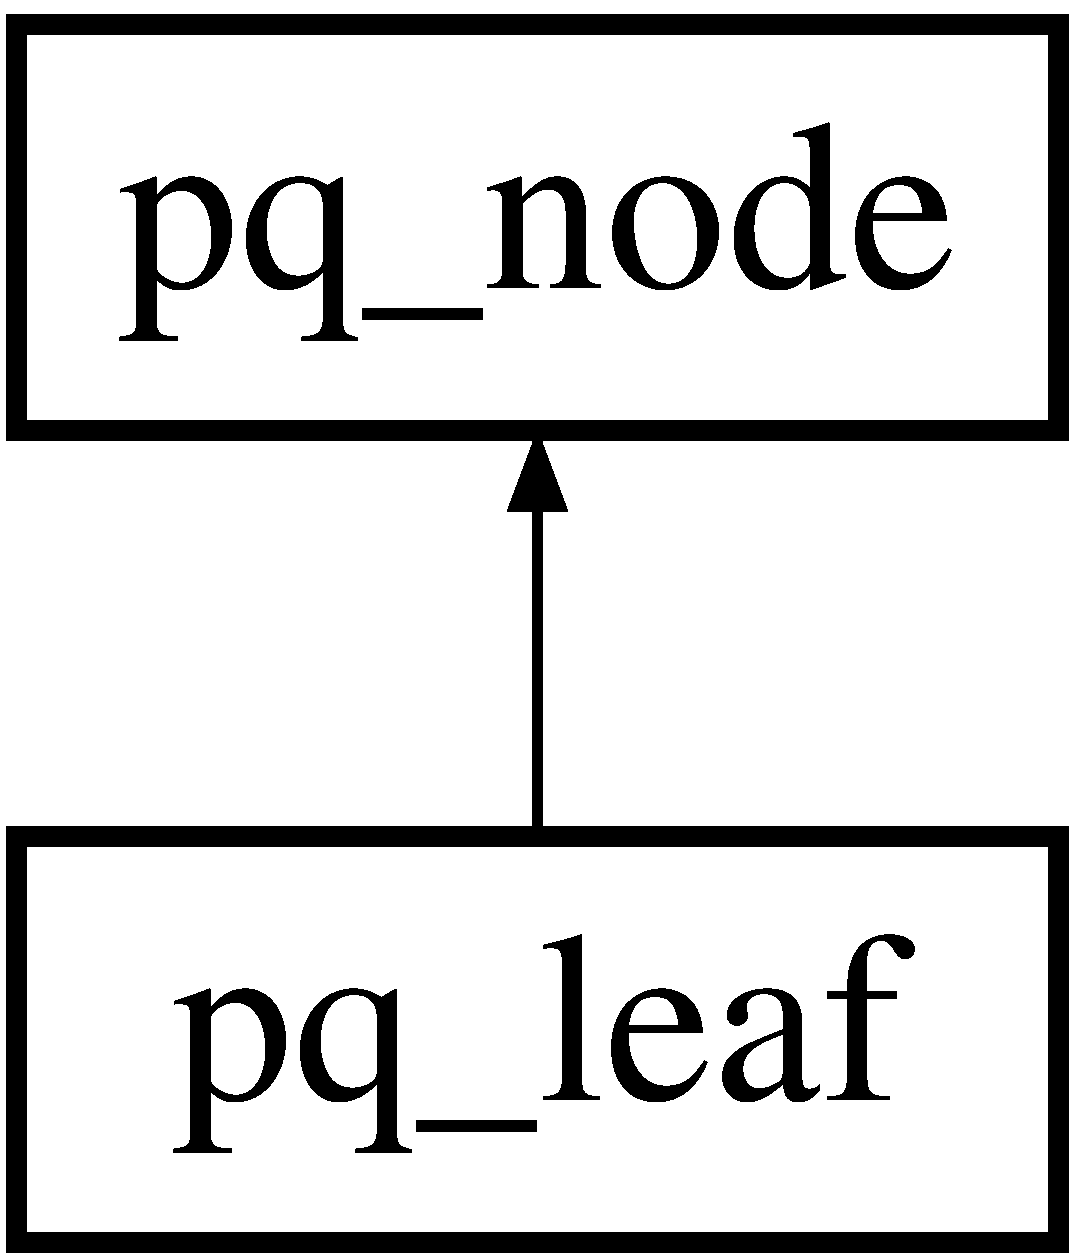
\includegraphics[height=2.000000cm]{classpq__leaf}
\end{center}
\end{figure}
\subsection*{Public Member Functions}
\begin{DoxyCompactItemize}
\item 
\mbox{\Hypertarget{classpq__leaf_a5478f8f28b4661ec404c492a01ac1f34}\label{classpq__leaf_a5478f8f28b4661ec404c492a01ac1f34}} 
{\bfseries pq\+\_\+leaf} (int, int, \mbox{\hyperlink{classedge}{edge}}, \mbox{\hyperlink{classnode}{node}})
\end{DoxyCompactItemize}
\subsection*{Friends}
\begin{DoxyCompactItemize}
\item 
\mbox{\Hypertarget{classpq__leaf_ab6a02224dbc06343d95919289aec77c8}\label{classpq__leaf_ab6a02224dbc06343d95919289aec77c8}} 
class {\bfseries planarity}
\item 
\mbox{\Hypertarget{classpq__leaf_a0a5be4bb438c891059fae98f607f2a9c}\label{classpq__leaf_a0a5be4bb438c891059fae98f607f2a9c}} 
class {\bfseries pq\+\_\+tree}
\end{DoxyCompactItemize}
\subsection*{Additional Inherited Members}


The documentation for this class was generated from the following files\+:\begin{DoxyCompactItemize}
\item 
include/\+K\+G\+L/pq\+\_\+node.\+h\item 
src/pq\+\_\+node.\+cpp\end{DoxyCompactItemize}

\hypertarget{classpq__node}{}\section{pq\+\_\+node Class Reference}
\label{classpq__node}\index{pq\+\_\+node@{pq\+\_\+node}}
Inheritance diagram for pq\+\_\+node\+:\begin{figure}[H]
\begin{center}
\leavevmode
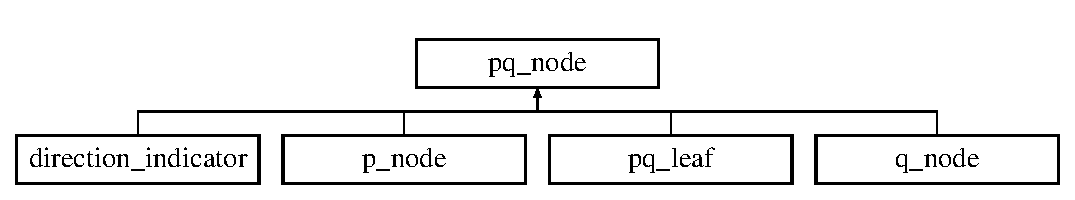
\includegraphics[height=2.000000cm]{classpq__node}
\end{center}
\end{figure}
\subsection*{Protected Types}
\begin{DoxyCompactItemize}
\item 
\mbox{\Hypertarget{classpq__node_a96827bdca8bf81d20213405dd27f8fa6}\label{classpq__node_a96827bdca8bf81d20213405dd27f8fa6}} 
enum {\bfseries P\+Q\+\_\+\+K\+I\+ND} \{ {\bfseries P\+\_\+\+N\+O\+DE}, 
{\bfseries Q\+\_\+\+N\+O\+DE}, 
{\bfseries L\+E\+AF}, 
{\bfseries D\+IR}
 \}
\item 
\mbox{\Hypertarget{classpq__node_a6236b20cd5f6cc02cb5f637ed34c96d9}\label{classpq__node_a6236b20cd5f6cc02cb5f637ed34c96d9}} 
enum {\bfseries P\+Q\+\_\+\+M\+A\+RK} \{ {\bfseries U\+N\+M\+A\+R\+K\+ED}, 
{\bfseries Q\+U\+E\+U\+ED}, 
{\bfseries B\+L\+O\+C\+K\+ED}, 
{\bfseries U\+N\+B\+L\+O\+C\+K\+ED}
 \}
\item 
\mbox{\Hypertarget{classpq__node_a34898c9eb1527787c07e8ebefd6bfba5}\label{classpq__node_a34898c9eb1527787c07e8ebefd6bfba5}} 
typedef \mbox{\hyperlink{classsymlist}{symlist}}$<$ \mbox{\hyperlink{classpq__node}{pq\+\_\+node}} $\ast$ $>$\+::\mbox{\hyperlink{structsymlist__iterator}{iterator}} {\bfseries iterator}
\end{DoxyCompactItemize}
\subsection*{Protected Member Functions}
\begin{DoxyCompactItemize}
\item 
\mbox{\Hypertarget{classpq__node_a75720c94fd6e2865ba24c76ff66b33b2}\label{classpq__node_a75720c94fd6e2865ba24c76ff66b33b2}} 
{\bfseries pq\+\_\+node} (\mbox{\hyperlink{classnode}{node}} n\+\_\+, int id\+\_\+)
\item 
\mbox{\Hypertarget{classpq__node_aa9873c0cfad88bc4404857ce57d422e4}\label{classpq__node_aa9873c0cfad88bc4404857ce57d422e4}} 
virtual P\+Q\+\_\+\+K\+I\+ND {\bfseries kind} () const =0
\item 
\mbox{\Hypertarget{classpq__node_aa6830ab47a280f41fe61b7d2f8b508bb}\label{classpq__node_aa6830ab47a280f41fe61b7d2f8b508bb}} 
virtual void {\bfseries partial} (\mbox{\hyperlink{structsymlist__iterator}{iterator}})
\item 
\mbox{\Hypertarget{classpq__node_af1ba861293e4493dba7cc2c9332fee76}\label{classpq__node_af1ba861293e4493dba7cc2c9332fee76}} 
virtual void {\bfseries full} (\mbox{\hyperlink{structsymlist__iterator}{iterator}})
\item 
\mbox{\Hypertarget{classpq__node_a66e00b01a0f49da14090dd8537b96816}\label{classpq__node_a66e00b01a0f49da14090dd8537b96816}} 
virtual void {\bfseries write} (ostream \&, int)=0
\item 
\mbox{\Hypertarget{classpq__node_a13100e0b030cc047f382d9ddf6a44f4a}\label{classpq__node_a13100e0b030cc047f382d9ddf6a44f4a}} 
virtual void {\bfseries clear} ()
\item 
\mbox{\Hypertarget{classpq__node_a72178a268ee1ece3ac106ac5fea3b12c}\label{classpq__node_a72178a268ee1ece3ac106ac5fea3b12c}} 
virtual \mbox{\hyperlink{classp__node}{p\+\_\+node}} $\ast$ {\bfseries P} ()=0
\item 
\mbox{\Hypertarget{classpq__node_aeeefcfcd19dbe4ca94e190006e8dd484}\label{classpq__node_aeeefcfcd19dbe4ca94e190006e8dd484}} 
virtual \mbox{\hyperlink{classq__node}{q\+\_\+node}} $\ast$ {\bfseries Q} ()=0
\item 
\mbox{\Hypertarget{classpq__node_a5c85bd25c32bb6f18d6d8d1bfd35f260}\label{classpq__node_a5c85bd25c32bb6f18d6d8d1bfd35f260}} 
virtual \mbox{\hyperlink{classdirection__indicator}{direction\+\_\+indicator}} $\ast$ {\bfseries D} ()=0
\item 
\mbox{\Hypertarget{classpq__node_a805b6ef48c847380b47c8ba882ed4ee2}\label{classpq__node_a805b6ef48c847380b47c8ba882ed4ee2}} 
virtual \mbox{\hyperlink{classpq__leaf}{pq\+\_\+leaf}} $\ast$ {\bfseries L} ()=0
\end{DoxyCompactItemize}
\subsection*{Protected Attributes}
\begin{DoxyCompactItemize}
\item 
\mbox{\Hypertarget{classpq__node_a8d8fb7b3059e7aeecf62eeed34076afb}\label{classpq__node_a8d8fb7b3059e7aeecf62eeed34076afb}} 
int {\bfseries pert\+\_\+children}
\item 
\mbox{\Hypertarget{classpq__node_a3fb78609f93f41efd6826ed3169fc312}\label{classpq__node_a3fb78609f93f41efd6826ed3169fc312}} 
int {\bfseries pert\+\_\+leaves}
\item 
\mbox{\Hypertarget{classpq__node_a058dda3d1197dfd2b343d1983d305d79}\label{classpq__node_a058dda3d1197dfd2b343d1983d305d79}} 
bool {\bfseries is\+\_\+endmost}
\item 
\mbox{\Hypertarget{classpq__node_a3e7c886498c76c633f057fb42ff9c435}\label{classpq__node_a3e7c886498c76c633f057fb42ff9c435}} 
\mbox{\hyperlink{classpq__node}{pq\+\_\+node}} $\ast$ {\bfseries father}
\item 
\mbox{\Hypertarget{classpq__node_aee913582a7b268ce2570bee8a8367c50}\label{classpq__node_aee913582a7b268ce2570bee8a8367c50}} 
P\+Q\+\_\+\+M\+A\+RK {\bfseries mark}
\item 
\mbox{\Hypertarget{classpq__node_a2cc030cfa4560872acea8b50ebd0542b}\label{classpq__node_a2cc030cfa4560872acea8b50ebd0542b}} 
\mbox{\hyperlink{classsymlist}{symlist}}$<$ \mbox{\hyperlink{classpq__node}{pq\+\_\+node}} $\ast$ $>$ {\bfseries sons}
\item 
\mbox{\Hypertarget{classpq__node_a5e8a5defa0fec4ff2e82fabee97296b4}\label{classpq__node_a5e8a5defa0fec4ff2e82fabee97296b4}} 
\mbox{\hyperlink{structsymlist__iterator}{iterator}} {\bfseries pos}
\item 
\mbox{\Hypertarget{classpq__node_a7eefcc531576365b720be9a28974b7b9}\label{classpq__node_a7eefcc531576365b720be9a28974b7b9}} 
list$<$ \mbox{\hyperlink{classpq__node}{pq\+\_\+node}} $\ast$ $>$\+::\mbox{\hyperlink{structsymlist__iterator}{iterator}} {\bfseries lpos}
\item 
\mbox{\Hypertarget{classpq__node_a4997fd09a95d9a659b99cea04197740a}\label{classpq__node_a4997fd09a95d9a659b99cea04197740a}} 
\mbox{\hyperlink{classnode}{node}} {\bfseries n}
\item 
\mbox{\Hypertarget{classpq__node_ad0034c1f93c3c77edb6d3a03f25aba06}\label{classpq__node_ad0034c1f93c3c77edb6d3a03f25aba06}} 
int {\bfseries id}
\item 
\mbox{\Hypertarget{classpq__node_ae6d5a236397b9a57159487eac7ec168d}\label{classpq__node_ae6d5a236397b9a57159487eac7ec168d}} 
\mbox{\hyperlink{classnode}{node}} {\bfseries up}
\item 
\mbox{\Hypertarget{classpq__node_a5a7bcdde1f57191a77a6a14994b38a50}\label{classpq__node_a5a7bcdde1f57191a77a6a14994b38a50}} 
int {\bfseries up\+\_\+id}
\end{DoxyCompactItemize}
\subsection*{Friends}
\begin{DoxyCompactItemize}
\item 
\mbox{\Hypertarget{classpq__node_ab10214fc73d6d72fa7ac390344a4fa46}\label{classpq__node_ab10214fc73d6d72fa7ac390344a4fa46}} 
class {\bfseries q\+\_\+node}
\item 
\mbox{\Hypertarget{classpq__node_a97e0a0034637eb5933f88c413aa715c6}\label{classpq__node_a97e0a0034637eb5933f88c413aa715c6}} 
class {\bfseries p\+\_\+node}
\item 
\mbox{\Hypertarget{classpq__node_a0a5be4bb438c891059fae98f607f2a9c}\label{classpq__node_a0a5be4bb438c891059fae98f607f2a9c}} 
class {\bfseries pq\+\_\+tree}
\item 
\mbox{\Hypertarget{classpq__node_ab6a02224dbc06343d95919289aec77c8}\label{classpq__node_ab6a02224dbc06343d95919289aec77c8}} 
class {\bfseries planarity}
\item 
\mbox{\Hypertarget{classpq__node_a2e8bee8ed51cc9d2567b69099c4d7cca}\label{classpq__node_a2e8bee8ed51cc9d2567b69099c4d7cca}} 
K\+G\+L\+\_\+\+E\+X\+T\+E\+RN friend ostream \& {\bfseries operator$<$$<$} (ostream \&, const \mbox{\hyperlink{classpq__tree}{pq\+\_\+tree}} \&)
\end{DoxyCompactItemize}


The documentation for this class was generated from the following files\+:\begin{DoxyCompactItemize}
\item 
include/\+K\+G\+L/pq\+\_\+node.\+h\item 
src/pq\+\_\+node.\+cpp\end{DoxyCompactItemize}

\hypertarget{classpq__tree}{}\section{pq\+\_\+tree Class Reference}
\label{classpq__tree}\index{pq\+\_\+tree@{pq\+\_\+tree}}


P\+Q-\/\+Trees.  




{\ttfamily \#include $<$pq\+\_\+tree.\+h$>$}

\subsection*{Public Types}
\begin{DoxyCompactItemize}
\item 
\mbox{\Hypertarget{classpq__tree_a241e516724fdb5ca21239772164458f3}\label{classpq__tree_a241e516724fdb5ca21239772164458f3}} 
typedef \mbox{\hyperlink{classsymlist}{symlist}}$<$ \mbox{\hyperlink{classpq__node}{pq\+\_\+node}} $\ast$ $>$ {\bfseries sons\+\_\+list}
\item 
\mbox{\Hypertarget{classpq__tree_ab47263066d4b0acc70e00043870d748a}\label{classpq__tree_ab47263066d4b0acc70e00043870d748a}} 
typedef \mbox{\hyperlink{classsymlist}{symlist}}$<$ \mbox{\hyperlink{classpq__node}{pq\+\_\+node}} $\ast$ $>$\+::iterator {\bfseries sons\+\_\+iterator}
\end{DoxyCompactItemize}
\subsection*{Public Member Functions}
\begin{DoxyCompactItemize}
\item 
\mbox{\Hypertarget{classpq__tree_afea06921780eb07ddb36294b109964d0}\label{classpq__tree_afea06921780eb07ddb36294b109964d0}} 
\mbox{\hyperlink{classpq__tree_afea06921780eb07ddb36294b109964d0}{pq\+\_\+tree}} ()
\begin{DoxyCompactList}\small\item\em Creates empty \mbox{\hyperlink{classpq__tree}{pq\+\_\+tree}}. \end{DoxyCompactList}\item 
\mbox{\hyperlink{classpq__tree_a2929a77b0e62274989884fd63db7fbe1}{pq\+\_\+tree}} (int id, \mbox{\hyperlink{classnode}{node}} n, const list$<$ \mbox{\hyperlink{classpq__leaf}{pq\+\_\+leaf}} $\ast$$>$ \&le)
\begin{DoxyCompactList}\small\item\em Creates a P\+Q-\/tree consisting of a single P-\/node whose whose children are the leaves given in list {\ttfamily le}. \end{DoxyCompactList}\item 
\mbox{\Hypertarget{classpq__tree_ae6b44b3a6db8914beb368aee2bf7cc92}\label{classpq__tree_ae6b44b3a6db8914beb368aee2bf7cc92}} 
\mbox{\hyperlink{classpq__tree_ae6b44b3a6db8914beb368aee2bf7cc92}{$\sim$pq\+\_\+tree}} ()
\begin{DoxyCompactList}\small\item\em Deletes P\+Q-\/tree. \end{DoxyCompactList}\item 
bool \mbox{\hyperlink{classpq__tree_a89b995f33c70db329b5e0cdd2ebe12b0}{reduce}} (list$<$ \mbox{\hyperlink{classpq__leaf}{pq\+\_\+leaf}} $\ast$$>$ \&leaves)
\begin{DoxyCompactList}\small\item\em Applies so called template matchings to the tree until either all leaves labeled with {\ttfamily id} are consecutive in all equivalent trees or until it is recognized that this can\textquotesingle{}t be achieved. \end{DoxyCompactList}\item 
void \mbox{\hyperlink{classpq__tree_ae201bdcb7bb1d53f36685c7c35b8d9dd}{replace\+\_\+pert}} (int id, \mbox{\hyperlink{classnode}{node}} n, const list$<$ \mbox{\hyperlink{classpq__leaf}{pq\+\_\+leaf}} $\ast$$>$ \&le, \mbox{\hyperlink{classplanar__embedding}{planar\+\_\+embedding}} $\ast$em=0, list$<$ \mbox{\hyperlink{classdirection__indicator}{direction\+\_\+indicator}} $>$ $\ast$dirs=0)
\begin{DoxyCompactList}\small\item\em Replaces all the pertinent parts of the P\+Q-\/tree after a (successful) reduction by a new P-\/node, whose children are given in {\ttfamily le}. \end{DoxyCompactList}\item 
void \mbox{\hyperlink{classpq__tree_a37f329b20436db734e9a73e3840d7521}{get\+\_\+frontier}} (\mbox{\hyperlink{classplanar__embedding}{planar\+\_\+embedding}} \&em, list$<$ \mbox{\hyperlink{classdirection__indicator}{direction\+\_\+indicator}} $>$ \&dirs)
\begin{DoxyCompactList}\small\item\em Scans whole tree from left to right and stores edges (in the graph) represented by the leaves in {\ttfamily em}. \end{DoxyCompactList}\item 
\mbox{\Hypertarget{classpq__tree_a1e2bdfb9af85972e9254260d74c63651}\label{classpq__tree_a1e2bdfb9af85972e9254260d74c63651}} 
void \mbox{\hyperlink{classpq__tree_a1e2bdfb9af85972e9254260d74c63651}{reset}} ()
\begin{DoxyCompactList}\small\item\em After a (successful) reduction {\ttfamily reset} has to be called in order to prepare the tree for the next reduction. \end{DoxyCompactList}\item 
\mbox{\hyperlink{classpq__node}{pq\+\_\+node}} $\ast$ \mbox{\hyperlink{classpq__tree_ad5788903c1411626e69e49aaa1b6541b}{get\+\_\+fail}} ()
\begin{DoxyCompactList}\small\item\em Returns the (P\+Q-\/) node to which none of the template matchings were applicable. \end{DoxyCompactList}\item 
bool \mbox{\hyperlink{classpq__tree_ab320f9d84cba3198a95cc5f33fde0813}{is\+\_\+fail\+\_\+root}} ()
\begin{DoxyCompactList}\small\item\em Returns true iff fail is the root of the pertinent subtree. \end{DoxyCompactList}\item 
\mbox{\hyperlink{structsymlist__iterator}{sons\+\_\+iterator}} \mbox{\hyperlink{classpq__tree_a68737f5cebd17670d9b73b797ca01a74}{remove\+\_\+dir\+\_\+ind}} (\mbox{\hyperlink{classq__node}{q\+\_\+node}} $\ast$q\+\_\+fail, \mbox{\hyperlink{structsymlist__iterator}{sons\+\_\+iterator}} s\+\_\+it)
\begin{DoxyCompactList}\small\item\em Remove a direction indicator among sons of a Q-\/node. Needed for computation of the obstruction set. \end{DoxyCompactList}\item 
bool \mbox{\hyperlink{classpq__tree_a170813af06d7b02083c3a7785e080de5}{integrity\+\_\+check}} () const
\begin{DoxyCompactList}\small\item\em Checks the structure of the tree. \end{DoxyCompactList}\end{DoxyCompactItemize}
\subsection*{Friends}
\begin{DoxyCompactItemize}
\item 
\mbox{\Hypertarget{classpq__tree_a2e8bee8ed51cc9d2567b69099c4d7cca}\label{classpq__tree_a2e8bee8ed51cc9d2567b69099c4d7cca}} 
K\+G\+L\+\_\+\+E\+X\+T\+E\+RN friend ostream \& {\bfseries operator$<$$<$} (ostream \&, const \mbox{\hyperlink{classpq__tree}{pq\+\_\+tree}} \&)
\end{DoxyCompactItemize}


\subsection{Detailed Description}
P\+Q-\/\+Trees. 

\begin{DoxyParagraph}{Date}
2019/05/07 18\+:17\+:08 
\end{DoxyParagraph}
\begin{DoxyParagraph}{Revision}
1.\+20 
\end{DoxyParagraph}


\subsection{Constructor \& Destructor Documentation}
\mbox{\Hypertarget{classpq__tree_a2929a77b0e62274989884fd63db7fbe1}\label{classpq__tree_a2929a77b0e62274989884fd63db7fbe1}} 
\index{pq\+\_\+tree@{pq\+\_\+tree}!pq\+\_\+tree@{pq\+\_\+tree}}
\index{pq\+\_\+tree@{pq\+\_\+tree}!pq\+\_\+tree@{pq\+\_\+tree}}
\subsubsection{\texorpdfstring{pq\+\_\+tree()}{pq\_tree()}}
{\footnotesize\ttfamily \+\_\+\+\_\+\+K\+G\+L\+\_\+\+B\+E\+G\+I\+N\+\_\+\+N\+A\+M\+E\+S\+P\+A\+CE pq\+\_\+tree\+::pq\+\_\+tree (\begin{DoxyParamCaption}\item[{int}]{id,  }\item[{\mbox{\hyperlink{classnode}{node}}}]{n,  }\item[{const list$<$ \mbox{\hyperlink{classpq__leaf}{pq\+\_\+leaf}} $\ast$$>$ \&}]{le }\end{DoxyParamCaption})}



Creates a P\+Q-\/tree consisting of a single P-\/node whose whose children are the leaves given in list {\ttfamily le}. 


\begin{DoxyParams}{Parameters}
{\em id} & st-\/number of {\ttfamily n} \\
\hline
{\em n} & node in the graph to which the P-\/node refers \\
\hline
{\em le} & list of children \\
\hline
\end{DoxyParams}


\subsection{Member Function Documentation}
\mbox{\Hypertarget{classpq__tree_ad5788903c1411626e69e49aaa1b6541b}\label{classpq__tree_ad5788903c1411626e69e49aaa1b6541b}} 
\index{pq\+\_\+tree@{pq\+\_\+tree}!get\+\_\+fail@{get\+\_\+fail}}
\index{get\+\_\+fail@{get\+\_\+fail}!pq\+\_\+tree@{pq\+\_\+tree}}
\subsubsection{\texorpdfstring{get\+\_\+fail()}{get\_fail()}}
{\footnotesize\ttfamily \mbox{\hyperlink{classpq__node}{pq\+\_\+node}}$\ast$ pq\+\_\+tree\+::get\+\_\+fail (\begin{DoxyParamCaption}{ }\end{DoxyParamCaption})\hspace{0.3cm}{\ttfamily [inline]}}



Returns the (P\+Q-\/) node to which none of the template matchings were applicable. 

\begin{DoxyReturn}{Returns}
P\+Q-\/node at which the reduction failed 
\end{DoxyReturn}
\mbox{\Hypertarget{classpq__tree_a37f329b20436db734e9a73e3840d7521}\label{classpq__tree_a37f329b20436db734e9a73e3840d7521}} 
\index{pq\+\_\+tree@{pq\+\_\+tree}!get\+\_\+frontier@{get\+\_\+frontier}}
\index{get\+\_\+frontier@{get\+\_\+frontier}!pq\+\_\+tree@{pq\+\_\+tree}}
\subsubsection{\texorpdfstring{get\+\_\+frontier()}{get\_frontier()}}
{\footnotesize\ttfamily void pq\+\_\+tree\+::get\+\_\+frontier (\begin{DoxyParamCaption}\item[{\mbox{\hyperlink{classplanar__embedding}{planar\+\_\+embedding}} \&}]{em,  }\item[{list$<$ \mbox{\hyperlink{classdirection__indicator}{direction\+\_\+indicator}} $>$ \&}]{dirs }\end{DoxyParamCaption})}



Scans whole tree from left to right and stores edges (in the graph) represented by the leaves in {\ttfamily em}. 

All direction indicators in the tree are stored in {\ttfamily dirs}. This is used in planarity test to get the upward embedding of the last node, because no reduction is needed in this case since all leaves are labeled with the same number.


\begin{DoxyParams}{Parameters}
{\em em} & planar embedding \\
\hline
{\em dirs} & direction indicators in tree \\
\hline
\end{DoxyParams}
\mbox{\Hypertarget{classpq__tree_a170813af06d7b02083c3a7785e080de5}\label{classpq__tree_a170813af06d7b02083c3a7785e080de5}} 
\index{pq\+\_\+tree@{pq\+\_\+tree}!integrity\+\_\+check@{integrity\+\_\+check}}
\index{integrity\+\_\+check@{integrity\+\_\+check}!pq\+\_\+tree@{pq\+\_\+tree}}
\subsubsection{\texorpdfstring{integrity\+\_\+check()}{integrity\_check()}}
{\footnotesize\ttfamily bool pq\+\_\+tree\+::integrity\+\_\+check (\begin{DoxyParamCaption}{ }\end{DoxyParamCaption}) const}



Checks the structure of the tree. 

\begin{DoxyNote}{Note}
Use this only for debugging since it scans the whole tree, which isn\textquotesingle{}t acceptable in terms of performance in most cases.
\end{DoxyNote}

\begin{DoxyRetVals}{Return values}
{\em true} & iff tree passes checks \\
\hline
\end{DoxyRetVals}
\mbox{\Hypertarget{classpq__tree_ab320f9d84cba3198a95cc5f33fde0813}\label{classpq__tree_ab320f9d84cba3198a95cc5f33fde0813}} 
\index{pq\+\_\+tree@{pq\+\_\+tree}!is\+\_\+fail\+\_\+root@{is\+\_\+fail\+\_\+root}}
\index{is\+\_\+fail\+\_\+root@{is\+\_\+fail\+\_\+root}!pq\+\_\+tree@{pq\+\_\+tree}}
\subsubsection{\texorpdfstring{is\+\_\+fail\+\_\+root()}{is\_fail\_root()}}
{\footnotesize\ttfamily bool pq\+\_\+tree\+::is\+\_\+fail\+\_\+root (\begin{DoxyParamCaption}{ }\end{DoxyParamCaption})\hspace{0.3cm}{\ttfamily [inline]}}



Returns true iff fail is the root of the pertinent subtree. 


\begin{DoxyRetVals}{Return values}
{\em true} & iff reduction failed at the root of the pertinent subtree. \\
\hline
\end{DoxyRetVals}
\mbox{\Hypertarget{classpq__tree_a89b995f33c70db329b5e0cdd2ebe12b0}\label{classpq__tree_a89b995f33c70db329b5e0cdd2ebe12b0}} 
\index{pq\+\_\+tree@{pq\+\_\+tree}!reduce@{reduce}}
\index{reduce@{reduce}!pq\+\_\+tree@{pq\+\_\+tree}}
\subsubsection{\texorpdfstring{reduce()}{reduce()}}
{\footnotesize\ttfamily bool pq\+\_\+tree\+::reduce (\begin{DoxyParamCaption}\item[{list$<$ \mbox{\hyperlink{classpq__leaf}{pq\+\_\+leaf}} $\ast$$>$ \&}]{leaves }\end{DoxyParamCaption})}



Applies so called template matchings to the tree until either all leaves labeled with {\ttfamily id} are consecutive in all equivalent trees or until it is recognized that this can\textquotesingle{}t be achieved. 

This operation is guaranteed to perform in O(\+P\+P\+T), where P\+PT is the size of the so called {\itshape pruned} {\itshape pertinent} {\itshape subtree}, which can be constructed, by cutting away all the parts of the P\+Q-\/tree, that do not contain a leaf labeled with {\ttfamily id}.


\begin{DoxyParams}{Parameters}
{\em leaves} & list of full leaves\\
\hline
\end{DoxyParams}

\begin{DoxyRetVals}{Return values}
{\em true} & if tree was successfully reduced \\
\hline
{\em false} & if reduction failed \\
\hline
\end{DoxyRetVals}
\mbox{\Hypertarget{classpq__tree_a68737f5cebd17670d9b73b797ca01a74}\label{classpq__tree_a68737f5cebd17670d9b73b797ca01a74}} 
\index{pq\+\_\+tree@{pq\+\_\+tree}!remove\+\_\+dir\+\_\+ind@{remove\+\_\+dir\+\_\+ind}}
\index{remove\+\_\+dir\+\_\+ind@{remove\+\_\+dir\+\_\+ind}!pq\+\_\+tree@{pq\+\_\+tree}}
\subsubsection{\texorpdfstring{remove\+\_\+dir\+\_\+ind()}{remove\_dir\_ind()}}
{\footnotesize\ttfamily \mbox{\hyperlink{structsymlist__iterator}{pq\+\_\+tree\+::sons\+\_\+iterator}} pq\+\_\+tree\+::remove\+\_\+dir\+\_\+ind (\begin{DoxyParamCaption}\item[{\mbox{\hyperlink{classq__node}{q\+\_\+node}} $\ast$}]{q\+\_\+fail,  }\item[{\mbox{\hyperlink{structsymlist__iterator}{sons\+\_\+iterator}}}]{s\+\_\+it }\end{DoxyParamCaption})}



Remove a direction indicator among sons of a Q-\/node. Needed for computation of the obstruction set. 


\begin{DoxyParams}{Parameters}
{\em q\+\_\+fail} & the Q-\/node on which the reduction failed \\
\hline
{\em the} & position of the direction indicator among the sons\\
\hline
\end{DoxyParams}

\begin{DoxyRetVals}{Return values}
{\em next} & valid sons iterator \\
\hline
\end{DoxyRetVals}
\mbox{\Hypertarget{classpq__tree_ae201bdcb7bb1d53f36685c7c35b8d9dd}\label{classpq__tree_ae201bdcb7bb1d53f36685c7c35b8d9dd}} 
\index{pq\+\_\+tree@{pq\+\_\+tree}!replace\+\_\+pert@{replace\+\_\+pert}}
\index{replace\+\_\+pert@{replace\+\_\+pert}!pq\+\_\+tree@{pq\+\_\+tree}}
\subsubsection{\texorpdfstring{replace\+\_\+pert()}{replace\_pert()}}
{\footnotesize\ttfamily void pq\+\_\+tree\+::replace\+\_\+pert (\begin{DoxyParamCaption}\item[{int}]{id,  }\item[{\mbox{\hyperlink{classnode}{node}}}]{n,  }\item[{const list$<$ \mbox{\hyperlink{classpq__leaf}{pq\+\_\+leaf}} $\ast$$>$ \&}]{le,  }\item[{\mbox{\hyperlink{classplanar__embedding}{planar\+\_\+embedding}} $\ast$}]{em = {\ttfamily 0},  }\item[{list$<$ \mbox{\hyperlink{classdirection__indicator}{direction\+\_\+indicator}} $>$ $\ast$}]{dirs = {\ttfamily 0} }\end{DoxyParamCaption})}



Replaces all the pertinent parts of the P\+Q-\/tree after a (successful) reduction by a new P-\/node, whose children are given in {\ttfamily le}. 

The edges (in the graph), represented by the leaves are stored in left to right order in {\ttfamily em}\mbox{[}n\mbox{]} They form (up to reversion) the so called upward-\/embedding. A direction indicator representing the direction in which the leaves were scanned is added to the sons of the root of the pertinent subtree (if neccessary). All direction indicators in the pertinent subtree are stored in {\ttfamily dirs}.


\begin{DoxyParams}{Parameters}
{\em id} & st-\/number of {\ttfamily n} \\
\hline
{\em n} & node in the graph to which the new P-\/node refers \\
\hline
{\em le} & list of children \\
\hline
{\em em} & planar embedding \\
\hline
{\em dirs} & direction indicators in pertinent subtree \\
\hline
\end{DoxyParams}


The documentation for this class was generated from the following files\+:\begin{DoxyCompactItemize}
\item 
include/\+K\+G\+L/pq\+\_\+tree.\+h\item 
src/pq\+\_\+tree.\+cpp\end{DoxyCompactItemize}

\hypertarget{classq__node}{}\section{q\+\_\+node Class Reference}
\label{classq__node}\index{q\+\_\+node@{q\+\_\+node}}
Inheritance diagram for q\+\_\+node\+:\begin{figure}[H]
\begin{center}
\leavevmode
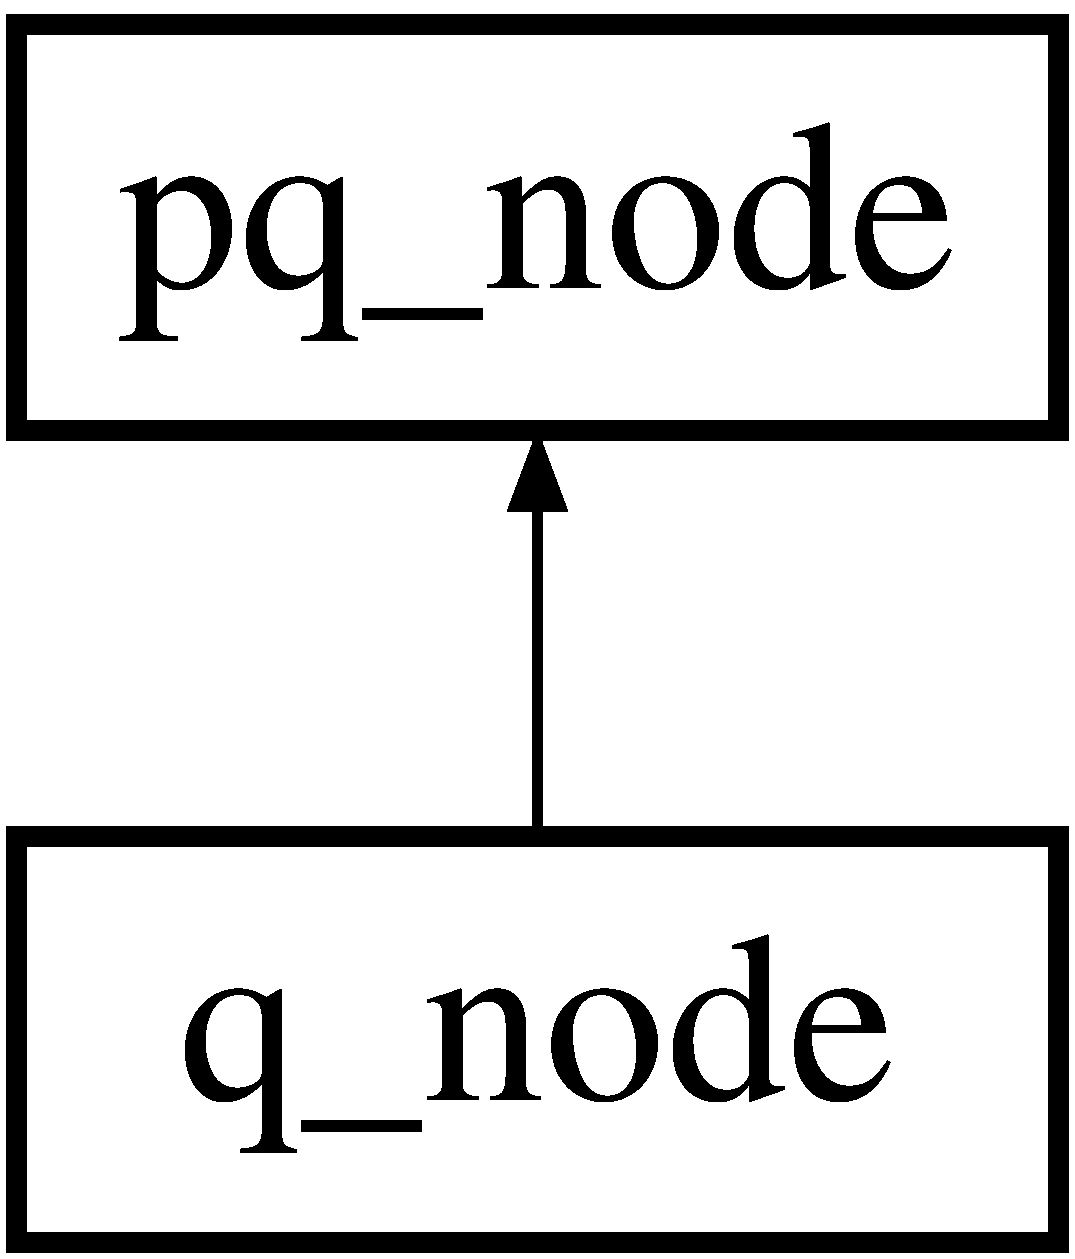
\includegraphics[height=2.000000cm]{classq__node}
\end{center}
\end{figure}
\subsection*{Friends}
\begin{DoxyCompactItemize}
\item 
\mbox{\Hypertarget{classq__node_ab6a02224dbc06343d95919289aec77c8}\label{classq__node_ab6a02224dbc06343d95919289aec77c8}} 
class {\bfseries planarity}
\item 
\mbox{\Hypertarget{classq__node_a0a5be4bb438c891059fae98f607f2a9c}\label{classq__node_a0a5be4bb438c891059fae98f607f2a9c}} 
class {\bfseries pq\+\_\+tree}
\end{DoxyCompactItemize}
\subsection*{Additional Inherited Members}


The documentation for this class was generated from the following files\+:\begin{DoxyCompactItemize}
\item 
include/\+K\+G\+L/pq\+\_\+node.\+h\item 
src/pq\+\_\+node.\+cpp\end{DoxyCompactItemize}

\hypertarget{classratio__cut__partition}{}\section{ratio\+\_\+cut\+\_\+partition Class Reference}
\label{classratio__cut__partition}\index{ratio\+\_\+cut\+\_\+partition@{ratio\+\_\+cut\+\_\+partition}}


Heuristic graph bi-\/partitioning algorithm (Wei-\/\+Cheng).  




{\ttfamily \#include $<$ratio\+\_\+cut\+\_\+partition.\+h$>$}

Inheritance diagram for ratio\+\_\+cut\+\_\+partition\+:\begin{figure}[H]
\begin{center}
\leavevmode
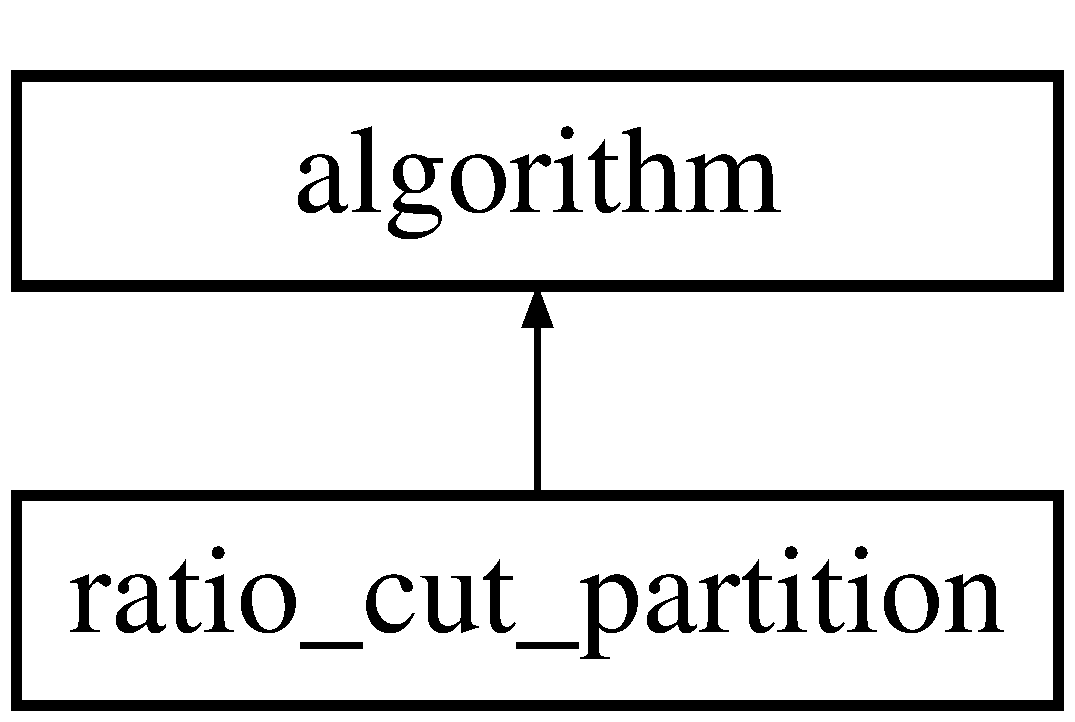
\includegraphics[height=2.000000cm]{classratio__cut__partition}
\end{center}
\end{figure}
\subsection*{Public Types}
\begin{DoxyCompactItemize}
\item 
typedef int \mbox{\hyperlink{classratio__cut__partition_ace53442bd0c1e21fbf00858ec6f6b456}{side\+\_\+type}}
\item 
typedef short int \mbox{\hyperlink{classratio__cut__partition_a558dda40abda8ab03edb4605dbb81e36}{fix\+\_\+type}}
\item 
typedef list$<$ \mbox{\hyperlink{classedge}{edge}} $>$\+::const\+\_\+iterator \mbox{\hyperlink{classratio__cut__partition_a5269af60e49810067411b085a1341adc}{cut\+\_\+edges\+\_\+iterator}}
\item 
typedef list$<$ \mbox{\hyperlink{classnode}{node}} $>$\+::const\+\_\+iterator \mbox{\hyperlink{classratio__cut__partition_a4f667099b56ded1bfef8f1fb4d09f81c}{nodes\+\_\+of\+\_\+one\+\_\+side\+\_\+iterator}}
\end{DoxyCompactItemize}
\subsection*{Public Member Functions}
\begin{DoxyCompactItemize}
\item 
\mbox{\hyperlink{classratio__cut__partition_a56e283d4ec5a06115146982e86c65878}{ratio\+\_\+cut\+\_\+partition}} ()
\item 
virtual \mbox{\hyperlink{classratio__cut__partition_a5fe4f3a926fd07a1af46cce9acdbb849}{$\sim$ratio\+\_\+cut\+\_\+partition}} ()
\item 
void \mbox{\hyperlink{classratio__cut__partition_a4c143f82aac5fee3b955414ab7d6ce19}{set\+\_\+vars}} (const \mbox{\hyperlink{classgraph}{graph}} \&G, const \mbox{\hyperlink{classnode__map}{node\+\_\+map}}$<$ int $>$ \&node\+\_\+weight, const \mbox{\hyperlink{classedge__map}{edge\+\_\+map}}$<$ int $>$ \&edge\+\_\+weight)
\item 
void \mbox{\hyperlink{classratio__cut__partition_aacd519cdb1760af792e22d57e746c07f}{set\+\_\+vars}} (const \mbox{\hyperlink{classgraph}{graph}} \&G, const \mbox{\hyperlink{classnode__map}{node\+\_\+map}}$<$ int $>$ \&node\+\_\+weight, const \mbox{\hyperlink{classedge__map}{edge\+\_\+map}}$<$ int $>$ \&edge\+\_\+weight, const \mbox{\hyperlink{classnode}{node}} source\+\_\+node, const \mbox{\hyperlink{classnode}{node}} target\+\_\+node)
\item 
void \mbox{\hyperlink{classratio__cut__partition_a67ea2ccb8b5cce2e4acd8e10e112a962}{set\+\_\+vars}} (const \mbox{\hyperlink{classgraph}{graph}} \&G, const \mbox{\hyperlink{classnode__map}{node\+\_\+map}}$<$ int $>$ \&node\+\_\+weight, const \mbox{\hyperlink{classedge__map}{edge\+\_\+map}}$<$ int $>$ \&edge\+\_\+weight, const \mbox{\hyperlink{classnode}{node}} source\+\_\+node, const \mbox{\hyperlink{classnode}{node}} target\+\_\+node, const \mbox{\hyperlink{classnode__map}{node\+\_\+map}}$<$ \mbox{\hyperlink{classratio__cut__partition_ace53442bd0c1e21fbf00858ec6f6b456}{side\+\_\+type}} $>$ \&init\+\_\+side)
\item 
void \mbox{\hyperlink{classratio__cut__partition_a2c09504b727a1b1d1e2f99a3a42de05b}{set\+\_\+vars}} (const \mbox{\hyperlink{classgraph}{graph}} \&G, const \mbox{\hyperlink{classnode__map}{node\+\_\+map}}$<$ int $>$ \&node\+\_\+weight, const \mbox{\hyperlink{classedge__map}{edge\+\_\+map}}$<$ int $>$ \&edge\+\_\+weight, const \mbox{\hyperlink{classnode}{node}} source\+\_\+node, const \mbox{\hyperlink{classnode}{node}} target\+\_\+node, const \mbox{\hyperlink{classnode__map}{node\+\_\+map}}$<$ \mbox{\hyperlink{classratio__cut__partition_a558dda40abda8ab03edb4605dbb81e36}{fix\+\_\+type}} $>$ \&fixed)
\item 
void \mbox{\hyperlink{classratio__cut__partition_a0ed59d80c7e15d2865d6aa4657ae3f78}{set\+\_\+vars}} (const \mbox{\hyperlink{classgraph}{graph}} \&G, const \mbox{\hyperlink{classnode__map}{node\+\_\+map}}$<$ int $>$ \&node\+\_\+weight, const \mbox{\hyperlink{classedge__map}{edge\+\_\+map}}$<$ int $>$ \&edge\+\_\+weight, const \mbox{\hyperlink{classnode}{node}} source\+\_\+node, const \mbox{\hyperlink{classnode}{node}} target\+\_\+node, const \mbox{\hyperlink{classnode__map}{node\+\_\+map}}$<$ \mbox{\hyperlink{classratio__cut__partition_ace53442bd0c1e21fbf00858ec6f6b456}{side\+\_\+type}} $>$ \&init\+\_\+side, const \mbox{\hyperlink{classnode__map}{node\+\_\+map}}$<$ \mbox{\hyperlink{classratio__cut__partition_a558dda40abda8ab03edb4605dbb81e36}{fix\+\_\+type}} $>$ \&fixed)
\item 
void \mbox{\hyperlink{classratio__cut__partition_af5a76fa0ecaf2c75792cc2c1574994c7}{store\+\_\+cut\+\_\+edges}} (const bool set)
\item 
void \mbox{\hyperlink{classratio__cut__partition_af0efdeab02cb235df47e2339c196051f}{store\+\_\+nodes\+AB}} (const bool set)
\item 
virtual int \mbox{\hyperlink{classratio__cut__partition_a469c613c69db19cb63e492075346fea2}{check}} (\mbox{\hyperlink{classgraph}{graph}} \&G)
\item 
int \mbox{\hyperlink{classratio__cut__partition_a4ab180ca4cf57c811e3478c3de4c4dc3}{run}} (\mbox{\hyperlink{classgraph}{graph}} \&G)
\item 
int \mbox{\hyperlink{classratio__cut__partition_a4fc9beab107546850974ffd5a47c1e7f}{get\+\_\+cutsize}} ()
\item 
double \mbox{\hyperlink{classratio__cut__partition_a9a61b2be36953d57e36fbb511cf1aa96}{get\+\_\+cutratio}} ()
\item 
\mbox{\hyperlink{classratio__cut__partition_ace53442bd0c1e21fbf00858ec6f6b456}{side\+\_\+type}} \mbox{\hyperlink{classratio__cut__partition_a3b0a7dcc26c9ca25016abf2cebf250fe}{get\+\_\+side\+\_\+of\+\_\+node}} (const \mbox{\hyperlink{classnode}{node}} \&n) const
\item 
\mbox{\hyperlink{classratio__cut__partition_ace53442bd0c1e21fbf00858ec6f6b456}{side\+\_\+type}} \mbox{\hyperlink{classratio__cut__partition_a47358935eb416c38969b66fbf3f095b5}{operator\mbox{[}$\,$\mbox{]}}} (const \mbox{\hyperlink{classnode}{node}} \&n) const
\item 
int \mbox{\hyperlink{classratio__cut__partition_af68528cd0b199718e6b2f5fe8182e779}{get\+\_\+weight\+\_\+on\+\_\+sideA}} (const \mbox{\hyperlink{classgraph}{graph}} \&G) const
\item 
int \mbox{\hyperlink{classratio__cut__partition_abd0835eeaec80f5ba56de5428985259f}{get\+\_\+weight\+\_\+on\+\_\+sideB}} (const \mbox{\hyperlink{classgraph}{graph}} \&G) const
\item 
\mbox{\hyperlink{classratio__cut__partition_a5269af60e49810067411b085a1341adc}{cut\+\_\+edges\+\_\+iterator}} \mbox{\hyperlink{classratio__cut__partition_a657a1d77b3b39037a52e6688674ad760}{cut\+\_\+edges\+\_\+begin}} () const
\item 
\mbox{\hyperlink{classratio__cut__partition_a5269af60e49810067411b085a1341adc}{cut\+\_\+edges\+\_\+iterator}} \mbox{\hyperlink{classratio__cut__partition_a8609d76a4d74cb3b2596ac370c839fce}{cut\+\_\+edges\+\_\+end}} () const
\item 
\mbox{\hyperlink{classratio__cut__partition_a4f667099b56ded1bfef8f1fb4d09f81c}{nodes\+\_\+of\+\_\+one\+\_\+side\+\_\+iterator}} \mbox{\hyperlink{classratio__cut__partition_a0c569bb7bd0a94269bd8938a2e0fce85}{nodes\+\_\+of\+\_\+side\+A\+\_\+begin}} () const
\item 
\mbox{\hyperlink{classratio__cut__partition_a4f667099b56ded1bfef8f1fb4d09f81c}{nodes\+\_\+of\+\_\+one\+\_\+side\+\_\+iterator}} \mbox{\hyperlink{classratio__cut__partition_a497d63a55cf326f62b97d0c77be094c7}{nodes\+\_\+of\+\_\+side\+A\+\_\+end}} () const
\item 
\mbox{\hyperlink{classratio__cut__partition_a4f667099b56ded1bfef8f1fb4d09f81c}{nodes\+\_\+of\+\_\+one\+\_\+side\+\_\+iterator}} \mbox{\hyperlink{classratio__cut__partition_ae36c08387ff6eae1236076cdbabf4fa5}{nodes\+\_\+of\+\_\+side\+B\+\_\+begin}} () const
\item 
\mbox{\hyperlink{classratio__cut__partition_a4f667099b56ded1bfef8f1fb4d09f81c}{nodes\+\_\+of\+\_\+one\+\_\+side\+\_\+iterator}} \mbox{\hyperlink{classratio__cut__partition_a838e3ab6d00155c1f3868cc920a4a8f6}{nodes\+\_\+of\+\_\+side\+B\+\_\+end}} () const
\item 
virtual void \mbox{\hyperlink{classratio__cut__partition_ad017eaf98f9ae4ca9dbe6b3eda9fc94d}{reset}} ()
\end{DoxyCompactItemize}
\subsection*{Static Public Attributes}
\begin{DoxyCompactItemize}
\item 
static const \mbox{\hyperlink{classratio__cut__partition_ace53442bd0c1e21fbf00858ec6f6b456}{side\+\_\+type}} \mbox{\hyperlink{classratio__cut__partition_ae1a3cd1c2ede82023f9a229e40909139}{A}} = 0
\item 
static const \mbox{\hyperlink{classratio__cut__partition_ace53442bd0c1e21fbf00858ec6f6b456}{side\+\_\+type}} \mbox{\hyperlink{classratio__cut__partition_adf075987228d8adc7950d5b1ba332daa}{B}} = 1
\item 
static const \mbox{\hyperlink{classratio__cut__partition_a558dda40abda8ab03edb4605dbb81e36}{fix\+\_\+type}} \mbox{\hyperlink{classratio__cut__partition_a2fe155c63de19dc08c16bcb382f0dcbc}{F\+I\+XA}} = 0
\item 
static const \mbox{\hyperlink{classratio__cut__partition_a558dda40abda8ab03edb4605dbb81e36}{fix\+\_\+type}} \mbox{\hyperlink{classratio__cut__partition_aea621a2460229773cbc095814942963a}{F\+I\+XB}} = 1
\item 
static const \mbox{\hyperlink{classratio__cut__partition_a558dda40abda8ab03edb4605dbb81e36}{fix\+\_\+type}} \mbox{\hyperlink{classratio__cut__partition_a153cc7e51ac5d72a00671b6bdbcc6fa5}{U\+N\+F\+I\+X\+ED}} = 2
\end{DoxyCompactItemize}
\subsection*{Protected Types}
\begin{DoxyCompactItemize}
\item 
\mbox{\Hypertarget{classratio__cut__partition_a8e2de20fc9f5cbe941aefa1c21c9b5ca}\label{classratio__cut__partition_a8e2de20fc9f5cbe941aefa1c21c9b5ca}} 
enum {\bfseries direction\+\_\+type} \{ {\bfseries L\+E\+F\+T\+\_\+\+S\+H\+I\+FT} = 2, 
{\bfseries R\+I\+G\+H\+T\+\_\+\+S\+H\+I\+FT} = 3
 \}
\end{DoxyCompactItemize}
\subsection*{Protected Member Functions}
\begin{DoxyCompactItemize}
\item 
\mbox{\Hypertarget{classratio__cut__partition_a04bea9656188ed01612106d797d1fd47}\label{classratio__cut__partition_a04bea9656188ed01612106d797d1fd47}} 
void {\bfseries divide\+\_\+up} (const \mbox{\hyperlink{classgraph}{graph}} \&G)
\item 
\mbox{\Hypertarget{classratio__cut__partition_a20a50609115998baaa361627a5a1ca79}\label{classratio__cut__partition_a20a50609115998baaa361627a5a1ca79}} 
void {\bfseries make\+\_\+connected} (\mbox{\hyperlink{classgraph}{graph}} \&G, list$<$ \mbox{\hyperlink{classedge}{edge}} $>$ \&artificial\+\_\+edges)
\item 
\mbox{\Hypertarget{classratio__cut__partition_afe0ee5301d84ba30787cffaf66583537}\label{classratio__cut__partition_afe0ee5301d84ba30787cffaf66583537}} 
void {\bfseries restore} (\mbox{\hyperlink{classgraph}{graph}} \&G, list$<$ \mbox{\hyperlink{classedge}{edge}} $>$ \&artificial\+\_\+edges)
\item 
\mbox{\Hypertarget{classratio__cut__partition_af4723810ece28284c79001b9ccf42ca4}\label{classratio__cut__partition_af4723810ece28284c79001b9ccf42ca4}} 
void {\bfseries initialization} (const \mbox{\hyperlink{classgraph}{graph}} \&G)
\item 
\mbox{\Hypertarget{classratio__cut__partition_a53b8ad2845ed39cc2677721c747bdce6}\label{classratio__cut__partition_a53b8ad2845ed39cc2677721c747bdce6}} 
void {\bfseries init\+\_\+data\+\_\+structure} (const \mbox{\hyperlink{classgraph}{graph}} \&G)
\item 
\mbox{\Hypertarget{classratio__cut__partition_a19fc538dbdaf8b1e0810a5bcde348c38}\label{classratio__cut__partition_a19fc538dbdaf8b1e0810a5bcde348c38}} 
void {\bfseries init\+\_\+filling\+\_\+buckets} (const \mbox{\hyperlink{classgraph}{graph}} \&G)
\item 
\mbox{\Hypertarget{classratio__cut__partition_a0f2caf60f5a9be58c983c84655537d51}\label{classratio__cut__partition_a0f2caf60f5a9be58c983c84655537d51}} 
int {\bfseries inital\+\_\+gain\+\_\+of\+\_\+node\+\_\+on\+\_\+sideA} (const \mbox{\hyperlink{classnode}{node}} cur\+\_\+node)
\item 
\mbox{\Hypertarget{classratio__cut__partition_ab1c602d2c984844f9fe51c4a889327c4}\label{classratio__cut__partition_ab1c602d2c984844f9fe51c4a889327c4}} 
int {\bfseries inital\+\_\+gain\+\_\+of\+\_\+node\+\_\+on\+\_\+sideB} (const \mbox{\hyperlink{classnode}{node}} cur\+\_\+node)
\item 
\mbox{\Hypertarget{classratio__cut__partition_ab3054dcfbcd012aba57218fa6d0c471b}\label{classratio__cut__partition_ab3054dcfbcd012aba57218fa6d0c471b}} 
void {\bfseries init\+\_\+variables} (const \mbox{\hyperlink{classgraph}{graph}} \&G)
\item 
\mbox{\Hypertarget{classratio__cut__partition_af83d8fc26a0836f4852af5f1db1aff5b}\label{classratio__cut__partition_af83d8fc26a0836f4852af5f1db1aff5b}} 
void {\bfseries compute\+\_\+max\+\_\+vertex\+\_\+degree} (const \mbox{\hyperlink{classgraph}{graph}} \&G)
\item 
\mbox{\Hypertarget{classratio__cut__partition_a7d3397f85318f781fbae287037e0ae33}\label{classratio__cut__partition_a7d3397f85318f781fbae287037e0ae33}} 
void {\bfseries determine\+\_\+source\+\_\+node} (const \mbox{\hyperlink{classgraph}{graph}} \&G)
\item 
\mbox{\Hypertarget{classratio__cut__partition_ae9a09532c706835e47ee4f02c24c82af}\label{classratio__cut__partition_ae9a09532c706835e47ee4f02c24c82af}} 
void {\bfseries compute\+\_\+target\+\_\+node} (const \mbox{\hyperlink{classgraph}{graph}} \&G)
\item 
\mbox{\Hypertarget{classratio__cut__partition_a9b2ac474cfdeabd8a2c5cb42fcc97d26}\label{classratio__cut__partition_a9b2ac474cfdeabd8a2c5cb42fcc97d26}} 
void {\bfseries right\+\_\+shift\+\_\+op} (const \mbox{\hyperlink{classgraph}{graph}} \&G)
\item 
\mbox{\Hypertarget{classratio__cut__partition_af736bd4e468935c1b1642f78d3df665d}\label{classratio__cut__partition_af736bd4e468935c1b1642f78d3df665d}} 
void {\bfseries left\+\_\+shift\+\_\+op} (const \mbox{\hyperlink{classgraph}{graph}} \&G)
\item 
\mbox{\Hypertarget{classratio__cut__partition_a8988d72cd456e79243f0e1c1b03ed501}\label{classratio__cut__partition_a8988d72cd456e79243f0e1c1b03ed501}} 
bool {\bfseries move\+\_\+vertex\+\_\+\+A2B} (const \mbox{\hyperlink{classgraph}{graph}} \&G, \mbox{\hyperlink{classnode}{node}} \&moved\+\_\+node)
\item 
\mbox{\Hypertarget{classratio__cut__partition_ab192d7130a80b6acf7da704162c51e6c}\label{classratio__cut__partition_ab192d7130a80b6acf7da704162c51e6c}} 
bool {\bfseries move\+\_\+vertex\+\_\+\+B2A} (const \mbox{\hyperlink{classgraph}{graph}} \&G, \mbox{\hyperlink{classnode}{node}} \&moved\+\_\+node)
\item 
\mbox{\Hypertarget{classratio__cut__partition_a24a11a8c3a090c0022583108b9e08c07}\label{classratio__cut__partition_a24a11a8c3a090c0022583108b9e08c07}} 
\mbox{\hyperlink{classnode}{node}} {\bfseries compute\+\_\+highest\+\_\+ratio\+\_\+node} (list$<$ \mbox{\hyperlink{classnode}{node}} $>$ node\+\_\+list)
\item 
\mbox{\Hypertarget{classratio__cut__partition_a0adcba3c7847fcb62b607eebc334c503}\label{classratio__cut__partition_a0adcba3c7847fcb62b607eebc334c503}} 
double {\bfseries cutratio} ()
\item 
\mbox{\Hypertarget{classratio__cut__partition_add7d355bd4df2cf6fa77ddc791692c88}\label{classratio__cut__partition_add7d355bd4df2cf6fa77ddc791692c88}} 
double {\bfseries ratio\+\_\+of\+\_\+node\+\_\+\+A2B} (const \mbox{\hyperlink{classnode}{node}} cur\+\_\+node)
\item 
\mbox{\Hypertarget{classratio__cut__partition_a094de379f453978db56695d53f6bc536}\label{classratio__cut__partition_a094de379f453978db56695d53f6bc536}} 
double {\bfseries ratio\+\_\+of\+\_\+node\+\_\+\+B2A} (const \mbox{\hyperlink{classnode}{node}} cur\+\_\+node)
\item 
\mbox{\Hypertarget{classratio__cut__partition_a5cda26b908793b59881798d88b07344c}\label{classratio__cut__partition_a5cda26b908793b59881798d88b07344c}} 
int {\bfseries range\+\_\+up} (const int gain\+\_\+value) const
\item 
\mbox{\Hypertarget{classratio__cut__partition_a3933d3829218a58cfc8eef84981034a8}\label{classratio__cut__partition_a3933d3829218a58cfc8eef84981034a8}} 
int {\bfseries range\+\_\+down} (const int index) const
\item 
\mbox{\Hypertarget{classratio__cut__partition_acdb4b69b6c94f06f6997ccec296a281f}\label{classratio__cut__partition_acdb4b69b6c94f06f6997ccec296a281f}} 
void {\bfseries update\+\_\+data\+\_\+structure\+\_\+\+A2B} (const \mbox{\hyperlink{classnode}{node}} cur\+\_\+node, const bool init\+\_\+mode)
\item 
\mbox{\Hypertarget{classratio__cut__partition_a942a3a035f59f2ab0d1d62da3c878eb8}\label{classratio__cut__partition_a942a3a035f59f2ab0d1d62da3c878eb8}} 
void {\bfseries update\+\_\+data\+\_\+structure\+\_\+\+B2A} (const \mbox{\hyperlink{classnode}{node}} cur\+\_\+node, const bool init\+\_\+mode)
\item 
\mbox{\Hypertarget{classratio__cut__partition_acbd0608a7e5560a52c447711cb59a644}\label{classratio__cut__partition_acbd0608a7e5560a52c447711cb59a644}} 
void {\bfseries update\+\_\+bucketA} (const \mbox{\hyperlink{classnode}{node}} cur\+\_\+node, const int old\+\_\+gain, const int new\+\_\+gain, const bool init\+\_\+mode)
\item 
\mbox{\Hypertarget{classratio__cut__partition_abe5d474e6d99c7bb200071d6484b5358}\label{classratio__cut__partition_abe5d474e6d99c7bb200071d6484b5358}} 
void {\bfseries update\+\_\+bucketB} (const \mbox{\hyperlink{classnode}{node}} cur\+\_\+node, const int old\+\_\+gain, const int new\+\_\+gain, const bool init\+\_\+mode)
\item 
\mbox{\Hypertarget{classratio__cut__partition_afbe33417996a8e040d4d802a1116e134}\label{classratio__cut__partition_afbe33417996a8e040d4d802a1116e134}} 
void {\bfseries update\+\_\+max\+\_\+gain} (const \mbox{\hyperlink{classratio__cut__partition_ace53442bd0c1e21fbf00858ec6f6b456}{side\+\_\+type}} side)
\item 
\mbox{\Hypertarget{classratio__cut__partition_aa8e1c0cce3f126e1aa4a3aa8489986fa}\label{classratio__cut__partition_aa8e1c0cce3f126e1aa4a3aa8489986fa}} 
void {\bfseries clean\+\_\+step} (const \mbox{\hyperlink{classgraph}{graph}} \&G)
\item 
\mbox{\Hypertarget{classratio__cut__partition_a8662bd1471d93d270de1c99d32ff3534}\label{classratio__cut__partition_a8662bd1471d93d270de1c99d32ff3534}} 
void {\bfseries copy\+\_\+side\+\_\+node\+\_\+map} (const \mbox{\hyperlink{classgraph}{graph}} \&G, \mbox{\hyperlink{classnode__map}{node\+\_\+map}}$<$ \mbox{\hyperlink{classratio__cut__partition_ace53442bd0c1e21fbf00858ec6f6b456}{side\+\_\+type}} $>$ \&dest, const \mbox{\hyperlink{classnode__map}{node\+\_\+map}}$<$ \mbox{\hyperlink{classratio__cut__partition_ace53442bd0c1e21fbf00858ec6f6b456}{side\+\_\+type}} $>$ source) const
\item 
\mbox{\Hypertarget{classratio__cut__partition_a758382177ff8be996d0be78a3cca069b}\label{classratio__cut__partition_a758382177ff8be996d0be78a3cca069b}} 
void {\bfseries iterative\+\_\+shifting} (const \mbox{\hyperlink{classgraph}{graph}} \&G)
\item 
\mbox{\Hypertarget{classratio__cut__partition_ae257dadc6cea5aef11badb68eadba0a5}\label{classratio__cut__partition_ae257dadc6cea5aef11badb68eadba0a5}} 
void {\bfseries group\+\_\+swapping} (const \mbox{\hyperlink{classgraph}{graph}} \&G)
\item 
\mbox{\Hypertarget{classratio__cut__partition_a16997844577ee3284a2b6fddbbea8c37}\label{classratio__cut__partition_a16997844577ee3284a2b6fddbbea8c37}} 
bool {\bfseries move\+\_\+manager} (const \mbox{\hyperlink{classgraph}{graph}} \&G)
\item 
\mbox{\Hypertarget{classratio__cut__partition_a2dbe8b4e73ac88fe6a9a2403ca35eb3f}\label{classratio__cut__partition_a2dbe8b4e73ac88fe6a9a2403ca35eb3f}} 
bool {\bfseries move\+\_\+vertex} (const \mbox{\hyperlink{classgraph}{graph}} \&G, \mbox{\hyperlink{classnode}{node}} \&moved\+\_\+node)
\item 
\mbox{\Hypertarget{classratio__cut__partition_a5588508593940888323121b340b40477}\label{classratio__cut__partition_a5588508593940888323121b340b40477}} 
void {\bfseries compute\+\_\+cut\+\_\+edges} (const \mbox{\hyperlink{classgraph}{graph}} \&G)
\item 
\mbox{\Hypertarget{classratio__cut__partition_a39341e2459485a3f5367081ff208e769}\label{classratio__cut__partition_a39341e2459485a3f5367081ff208e769}} 
void {\bfseries compute\+\_\+nodes\+AB} (const \mbox{\hyperlink{classgraph}{graph}} \&G)
\end{DoxyCompactItemize}
\subsection*{Protected Attributes}
\begin{DoxyCompactItemize}
\item 
\mbox{\Hypertarget{classratio__cut__partition_a7f2ddebc25563a35cb6424f7a5d4b549}\label{classratio__cut__partition_a7f2ddebc25563a35cb6424f7a5d4b549}} 
bool {\bfseries enable\+\_\+cut\+\_\+edges\+\_\+storing}
\item 
\mbox{\Hypertarget{classratio__cut__partition_a6ab3992e4d1ca3c90f300b755b446a4a}\label{classratio__cut__partition_a6ab3992e4d1ca3c90f300b755b446a4a}} 
list$<$ \mbox{\hyperlink{classedge}{edge}} $>$ {\bfseries cut\+\_\+edges}
\item 
\mbox{\Hypertarget{classratio__cut__partition_a6dff7e2e6cecdc63147fdee71d876a34}\label{classratio__cut__partition_a6dff7e2e6cecdc63147fdee71d876a34}} 
bool {\bfseries enable\+\_\+nodes\+A\+B\+\_\+storing}
\item 
\mbox{\Hypertarget{classratio__cut__partition_af0d2db1c18136863b147b60b3dcdc98d}\label{classratio__cut__partition_af0d2db1c18136863b147b60b3dcdc98d}} 
list$<$ \mbox{\hyperlink{classnode}{node}} $>$ {\bfseries nodesA}
\item 
\mbox{\Hypertarget{classratio__cut__partition_aa70e7fe023b5bfe97797ac0c53980eb8}\label{classratio__cut__partition_aa70e7fe023b5bfe97797ac0c53980eb8}} 
list$<$ \mbox{\hyperlink{classnode}{node}} $>$ {\bfseries nodesB}
\item 
\mbox{\Hypertarget{classratio__cut__partition_abb18c3acafc590e258453d7a8d86bb49}\label{classratio__cut__partition_abb18c3acafc590e258453d7a8d86bb49}} 
\mbox{\hyperlink{classnode}{node}} {\bfseries source\+\_\+node}
\item 
\mbox{\Hypertarget{classratio__cut__partition_a343ba76869e64141fb795010e388744b}\label{classratio__cut__partition_a343ba76869e64141fb795010e388744b}} 
\mbox{\hyperlink{classnode}{node}} {\bfseries target\+\_\+node}
\item 
\mbox{\Hypertarget{classratio__cut__partition_aa722d032cb59664894c6301ceee86729}\label{classratio__cut__partition_aa722d032cb59664894c6301ceee86729}} 
bool {\bfseries set\+\_\+vars\+\_\+executed}
\item 
\mbox{\Hypertarget{classratio__cut__partition_a248512624766f0b21d154b4841c95a1d}\label{classratio__cut__partition_a248512624766f0b21d154b4841c95a1d}} 
bool {\bfseries provided\+\_\+st}
\item 
\mbox{\Hypertarget{classratio__cut__partition_a963258b950f7142e3cac714353b1b21e}\label{classratio__cut__partition_a963258b950f7142e3cac714353b1b21e}} 
bool {\bfseries provided\+\_\+initial\+\_\+part}
\item 
\mbox{\Hypertarget{classratio__cut__partition_a5f1f85feae589f7d39da48a412c90376}\label{classratio__cut__partition_a5f1f85feae589f7d39da48a412c90376}} 
bool {\bfseries provided\+\_\+fix}
\item 
\mbox{\Hypertarget{classratio__cut__partition_ad77023b9f60e88274bf54f2019404768}\label{classratio__cut__partition_ad77023b9f60e88274bf54f2019404768}} 
\mbox{\hyperlink{classnode__map}{node\+\_\+map}}$<$ \mbox{\hyperlink{classratio__cut__partition_a558dda40abda8ab03edb4605dbb81e36}{fix\+\_\+type}} $>$ {\bfseries fixed}
\item 
\mbox{\Hypertarget{classratio__cut__partition_a11141cdf8705dbb4331315591a3759d6}\label{classratio__cut__partition_a11141cdf8705dbb4331315591a3759d6}} 
direction\+\_\+type {\bfseries direction}
\item 
\mbox{\Hypertarget{classratio__cut__partition_a4d9d2a9317a062f839ea7155c37b173f}\label{classratio__cut__partition_a4d9d2a9317a062f839ea7155c37b173f}} 
\mbox{\hyperlink{classnode__map}{node\+\_\+map}}$<$ int $>$ {\bfseries node\+\_\+weight}
\item 
\mbox{\Hypertarget{classratio__cut__partition_a48a85c82fb09b83c9d494d6d1232fab2}\label{classratio__cut__partition_a48a85c82fb09b83c9d494d6d1232fab2}} 
\mbox{\hyperlink{classedge__map}{edge\+\_\+map}}$<$ int $>$ {\bfseries edge\+\_\+weight}
\item 
\mbox{\Hypertarget{classratio__cut__partition_a74193c82e8dc7d997780613378919106}\label{classratio__cut__partition_a74193c82e8dc7d997780613378919106}} 
int {\bfseries max\+\_\+edge\+\_\+weight}
\item 
\mbox{\Hypertarget{classratio__cut__partition_af1b839e48e498cf8ca93c8ec5df8a686}\label{classratio__cut__partition_af1b839e48e498cf8ca93c8ec5df8a686}} 
int {\bfseries node\+\_\+weight\+\_\+on\+\_\+sideA}
\item 
\mbox{\Hypertarget{classratio__cut__partition_aa16d1b508db86eb0ba4824642394999a}\label{classratio__cut__partition_aa16d1b508db86eb0ba4824642394999a}} 
int {\bfseries node\+\_\+weight\+\_\+on\+\_\+sideB}
\item 
\mbox{\Hypertarget{classratio__cut__partition_a7de51193b63e241afe263345479580ee}\label{classratio__cut__partition_a7de51193b63e241afe263345479580ee}} 
int {\bfseries nodes\+\_\+on\+\_\+sideA}
\item 
\mbox{\Hypertarget{classratio__cut__partition_a6b797912a7653537473e0e583a3f245a}\label{classratio__cut__partition_a6b797912a7653537473e0e583a3f245a}} 
int {\bfseries nodes\+\_\+on\+\_\+sideB}
\item 
\mbox{\Hypertarget{classratio__cut__partition_a2bf913d1d8607747885177a3b585e611}\label{classratio__cut__partition_a2bf913d1d8607747885177a3b585e611}} 
\mbox{\hyperlink{classnode__map}{node\+\_\+map}}$<$ \mbox{\hyperlink{classratio__cut__partition_ace53442bd0c1e21fbf00858ec6f6b456}{side\+\_\+type}} $>$ {\bfseries side}
\item 
\mbox{\Hypertarget{classratio__cut__partition_af22e9f52fdde7bfecbadd5446dc523a3}\label{classratio__cut__partition_af22e9f52fdde7bfecbadd5446dc523a3}} 
\mbox{\hyperlink{classnode__map}{node\+\_\+map}}$<$ list$<$ \mbox{\hyperlink{classnode}{node}} $>$\+::iterator $>$ {\bfseries position\+\_\+in\+\_\+bucket}
\item 
\mbox{\Hypertarget{classratio__cut__partition_ab07041983ab24ac059e8c98192c146e4}\label{classratio__cut__partition_ab07041983ab24ac059e8c98192c146e4}} 
int {\bfseries max\+\_\+vertex\+\_\+degree}
\item 
\mbox{\Hypertarget{classratio__cut__partition_a112bfcfb9d05d5bbdeb29576a61399e1}\label{classratio__cut__partition_a112bfcfb9d05d5bbdeb29576a61399e1}} 
\mbox{\hyperlink{classedge__map}{edge\+\_\+map}}$<$ int $>$ {\bfseries aside}
\item 
\mbox{\Hypertarget{classratio__cut__partition_ab9c1166efb1cbb65ff6c55bb6e3c9e6d}\label{classratio__cut__partition_ab9c1166efb1cbb65ff6c55bb6e3c9e6d}} 
\mbox{\hyperlink{classedge__map}{edge\+\_\+map}}$<$ int $>$ {\bfseries bside}
\item 
\mbox{\Hypertarget{classratio__cut__partition_a45966fb7dc3624c3829c8b0f7a389379}\label{classratio__cut__partition_a45966fb7dc3624c3829c8b0f7a389379}} 
\mbox{\hyperlink{classedge__map}{edge\+\_\+map}}$<$ list$<$ \mbox{\hyperlink{classnode}{node}} $>$ $>$ {\bfseries unlockedA}
\item 
\mbox{\Hypertarget{classratio__cut__partition_a6a3e407a15a02ddfc39ca42399f7b54a}\label{classratio__cut__partition_a6a3e407a15a02ddfc39ca42399f7b54a}} 
\mbox{\hyperlink{classedge__map}{edge\+\_\+map}}$<$ list$<$ \mbox{\hyperlink{classnode}{node}} $>$ $>$ {\bfseries unlockedB}
\item 
\mbox{\Hypertarget{classratio__cut__partition_af24ff191abbb0578f0bfc54fef5f6d45}\label{classratio__cut__partition_af24ff191abbb0578f0bfc54fef5f6d45}} 
\mbox{\hyperlink{classnode__map}{node\+\_\+map}}$<$ int $>$ {\bfseries gain\+\_\+value}
\item 
\mbox{\Hypertarget{classratio__cut__partition_a2e3f25066f798f28e9e5646f866ffc1c}\label{classratio__cut__partition_a2e3f25066f798f28e9e5646f866ffc1c}} 
bool {\bfseries bucket\+A\+\_\+empty}
\item 
\mbox{\Hypertarget{classratio__cut__partition_af4bbd571d19340f92519240b96b52702}\label{classratio__cut__partition_af4bbd571d19340f92519240b96b52702}} 
bool {\bfseries bucket\+B\+\_\+empty}
\item 
\mbox{\Hypertarget{classratio__cut__partition_ae69ef6876be68d5752d247564a524c6a}\label{classratio__cut__partition_ae69ef6876be68d5752d247564a524c6a}} 
int {\bfseries max\+\_\+gainA}
\item 
\mbox{\Hypertarget{classratio__cut__partition_af184ffdb46e49b1fc95faa1e6a91cc8e}\label{classratio__cut__partition_af184ffdb46e49b1fc95faa1e6a91cc8e}} 
int {\bfseries max\+\_\+gainB}
\item 
\mbox{\Hypertarget{classratio__cut__partition_ae344fc28ce1d559c793bc7cc113843b6}\label{classratio__cut__partition_ae344fc28ce1d559c793bc7cc113843b6}} 
vector$<$ list$<$ \mbox{\hyperlink{classnode}{node}} $>$ $>$ {\bfseries bucketA}
\item 
\mbox{\Hypertarget{classratio__cut__partition_abf8e49d7032714f10aac12cf635dcf77}\label{classratio__cut__partition_abf8e49d7032714f10aac12cf635dcf77}} 
vector$<$ list$<$ \mbox{\hyperlink{classnode}{node}} $>$ $>$ {\bfseries bucketB}
\item 
\mbox{\Hypertarget{classratio__cut__partition_aa01f2d6257fff28739e2431fe826ef71}\label{classratio__cut__partition_aa01f2d6257fff28739e2431fe826ef71}} 
int {\bfseries cur\+\_\+cutsize}
\item 
\mbox{\Hypertarget{classratio__cut__partition_a9dad324884cef5bcdd50122fc98e0860}\label{classratio__cut__partition_a9dad324884cef5bcdd50122fc98e0860}} 
double {\bfseries cur\+\_\+cutratio}
\end{DoxyCompactItemize}


\subsection{Detailed Description}
Heuristic graph bi-\/partitioning algorithm (Wei-\/\+Cheng). 

This class implements a heuristic graph bi-\/partitioning algorithm using the ratio cut method proposed by Y. C. Wei and C. K. Cheng in 1991.

In the case E is the set of edges of the graph, the algorithm needs {\ttfamily O($\vert$\+E$\vert$)} time to proceed.

\begin{DoxySeeAlso}{See also}
\mbox{\hyperlink{classfm__partition}{fm\+\_\+partition}} 
\end{DoxySeeAlso}


\subsection{Member Typedef Documentation}
\mbox{\Hypertarget{classratio__cut__partition_a5269af60e49810067411b085a1341adc}\label{classratio__cut__partition_a5269af60e49810067411b085a1341adc}} 
\index{ratio\+\_\+cut\+\_\+partition@{ratio\+\_\+cut\+\_\+partition}!cut\+\_\+edges\+\_\+iterator@{cut\+\_\+edges\+\_\+iterator}}
\index{cut\+\_\+edges\+\_\+iterator@{cut\+\_\+edges\+\_\+iterator}!ratio\+\_\+cut\+\_\+partition@{ratio\+\_\+cut\+\_\+partition}}
\subsubsection{\texorpdfstring{cut\+\_\+edges\+\_\+iterator}{cut\_edges\_iterator}}
{\footnotesize\ttfamily typedef list$<$\mbox{\hyperlink{classedge}{edge}}$>$\+::const\+\_\+iterator \mbox{\hyperlink{classratio__cut__partition_a5269af60e49810067411b085a1341adc}{ratio\+\_\+cut\+\_\+partition\+::cut\+\_\+edges\+\_\+iterator}}}

Iterator type for edges which belong to the cut. \mbox{\Hypertarget{classratio__cut__partition_a558dda40abda8ab03edb4605dbb81e36}\label{classratio__cut__partition_a558dda40abda8ab03edb4605dbb81e36}} 
\index{ratio\+\_\+cut\+\_\+partition@{ratio\+\_\+cut\+\_\+partition}!fix\+\_\+type@{fix\+\_\+type}}
\index{fix\+\_\+type@{fix\+\_\+type}!ratio\+\_\+cut\+\_\+partition@{ratio\+\_\+cut\+\_\+partition}}
\subsubsection{\texorpdfstring{fix\+\_\+type}{fix\_type}}
{\footnotesize\ttfamily typedef short int \mbox{\hyperlink{classratio__cut__partition_a558dda40abda8ab03edb4605dbb81e36}{ratio\+\_\+cut\+\_\+partition\+::fix\+\_\+type}}}

Fix type of each node (needed with \mbox{\hyperlink{classratio__cut__partition_a4c143f82aac5fee3b955414ab7d6ce19}{ratio\+\_\+cut\+\_\+partition\+::set\+\_\+vars}}).

\begin{DoxySeeAlso}{See also}
\mbox{\hyperlink{classratio__cut__partition_a2fe155c63de19dc08c16bcb382f0dcbc}{ratio\+\_\+cut\+\_\+partition\+::\+F\+I\+XA}} 

\mbox{\hyperlink{classratio__cut__partition_aea621a2460229773cbc095814942963a}{ratio\+\_\+cut\+\_\+partition\+::\+F\+I\+XB}} 

\mbox{\hyperlink{classratio__cut__partition_a153cc7e51ac5d72a00671b6bdbcc6fa5}{ratio\+\_\+cut\+\_\+partition\+::\+U\+N\+F\+I\+X\+ED}} 
\end{DoxySeeAlso}
\mbox{\Hypertarget{classratio__cut__partition_a4f667099b56ded1bfef8f1fb4d09f81c}\label{classratio__cut__partition_a4f667099b56ded1bfef8f1fb4d09f81c}} 
\index{ratio\+\_\+cut\+\_\+partition@{ratio\+\_\+cut\+\_\+partition}!nodes\+\_\+of\+\_\+one\+\_\+side\+\_\+iterator@{nodes\+\_\+of\+\_\+one\+\_\+side\+\_\+iterator}}
\index{nodes\+\_\+of\+\_\+one\+\_\+side\+\_\+iterator@{nodes\+\_\+of\+\_\+one\+\_\+side\+\_\+iterator}!ratio\+\_\+cut\+\_\+partition@{ratio\+\_\+cut\+\_\+partition}}
\subsubsection{\texorpdfstring{nodes\+\_\+of\+\_\+one\+\_\+side\+\_\+iterator}{nodes\_of\_one\_side\_iterator}}
{\footnotesize\ttfamily typedef list$<$\mbox{\hyperlink{classnode}{node}}$>$\+::const\+\_\+iterator \mbox{\hyperlink{classratio__cut__partition_a4f667099b56ded1bfef8f1fb4d09f81c}{ratio\+\_\+cut\+\_\+partition\+::nodes\+\_\+of\+\_\+one\+\_\+side\+\_\+iterator}}}

Iterator type for nodes of a side. \mbox{\Hypertarget{classratio__cut__partition_ace53442bd0c1e21fbf00858ec6f6b456}\label{classratio__cut__partition_ace53442bd0c1e21fbf00858ec6f6b456}} 
\index{ratio\+\_\+cut\+\_\+partition@{ratio\+\_\+cut\+\_\+partition}!side\+\_\+type@{side\+\_\+type}}
\index{side\+\_\+type@{side\+\_\+type}!ratio\+\_\+cut\+\_\+partition@{ratio\+\_\+cut\+\_\+partition}}
\subsubsection{\texorpdfstring{side\+\_\+type}{side\_type}}
{\footnotesize\ttfamily typedef int \mbox{\hyperlink{classratio__cut__partition_ace53442bd0c1e21fbf00858ec6f6b456}{ratio\+\_\+cut\+\_\+partition\+::side\+\_\+type}}}

Return type of \mbox{\hyperlink{classratio__cut__partition_a3b0a7dcc26c9ca25016abf2cebf250fe}{ratio\+\_\+cut\+\_\+partition\+::get\+\_\+side\+\_\+of\+\_\+node}}.

\begin{DoxySeeAlso}{See also}
\mbox{\hyperlink{classratio__cut__partition_ae1a3cd1c2ede82023f9a229e40909139}{ratio\+\_\+cut\+\_\+partition\+::A}} 

\mbox{\hyperlink{classratio__cut__partition_adf075987228d8adc7950d5b1ba332daa}{ratio\+\_\+cut\+\_\+partition\+::B}} 
\end{DoxySeeAlso}


\subsection{Constructor \& Destructor Documentation}
\mbox{\Hypertarget{classratio__cut__partition_a56e283d4ec5a06115146982e86c65878}\label{classratio__cut__partition_a56e283d4ec5a06115146982e86c65878}} 
\index{ratio\+\_\+cut\+\_\+partition@{ratio\+\_\+cut\+\_\+partition}!ratio\+\_\+cut\+\_\+partition@{ratio\+\_\+cut\+\_\+partition}}
\index{ratio\+\_\+cut\+\_\+partition@{ratio\+\_\+cut\+\_\+partition}!ratio\+\_\+cut\+\_\+partition@{ratio\+\_\+cut\+\_\+partition}}
\subsubsection{\texorpdfstring{ratio\+\_\+cut\+\_\+partition()}{ratio\_cut\_partition()}}
{\footnotesize\ttfamily ratio\+\_\+cut\+\_\+partition\+::ratio\+\_\+cut\+\_\+partition (\begin{DoxyParamCaption}{ }\end{DoxyParamCaption})}

Default constructor.

\begin{DoxySeeAlso}{See also}
\mbox{\hyperlink{classalgorithm_ab79e1ddec2f2afdf4b36b10724db8b15}{algorithm\+::algorithm}} 
\end{DoxySeeAlso}
\mbox{\Hypertarget{classratio__cut__partition_a5fe4f3a926fd07a1af46cce9acdbb849}\label{classratio__cut__partition_a5fe4f3a926fd07a1af46cce9acdbb849}} 
\index{ratio\+\_\+cut\+\_\+partition@{ratio\+\_\+cut\+\_\+partition}!````~ratio\+\_\+cut\+\_\+partition@{$\sim$ratio\+\_\+cut\+\_\+partition}}
\index{````~ratio\+\_\+cut\+\_\+partition@{$\sim$ratio\+\_\+cut\+\_\+partition}!ratio\+\_\+cut\+\_\+partition@{ratio\+\_\+cut\+\_\+partition}}
\subsubsection{\texorpdfstring{$\sim$ratio\+\_\+cut\+\_\+partition()}{~ratio\_cut\_partition()}}
{\footnotesize\ttfamily ratio\+\_\+cut\+\_\+partition\+::$\sim$ratio\+\_\+cut\+\_\+partition (\begin{DoxyParamCaption}{ }\end{DoxyParamCaption})\hspace{0.3cm}{\ttfamily [virtual]}}

Destructor.

\begin{DoxySeeAlso}{See also}
\mbox{\hyperlink{classalgorithm_adca9b1e7fa3afd914519a9dbb44e9fd5}{algorithm\+::$\sim$algorithm}} 
\end{DoxySeeAlso}


\subsection{Member Function Documentation}
\mbox{\Hypertarget{classratio__cut__partition_a469c613c69db19cb63e492075346fea2}\label{classratio__cut__partition_a469c613c69db19cb63e492075346fea2}} 
\index{ratio\+\_\+cut\+\_\+partition@{ratio\+\_\+cut\+\_\+partition}!check@{check}}
\index{check@{check}!ratio\+\_\+cut\+\_\+partition@{ratio\+\_\+cut\+\_\+partition}}
\subsubsection{\texorpdfstring{check()}{check()}}
{\footnotesize\ttfamily int ratio\+\_\+cut\+\_\+partition\+::check (\begin{DoxyParamCaption}\item[{\mbox{\hyperlink{classgraph}{graph}} \&}]{G }\end{DoxyParamCaption})\hspace{0.3cm}{\ttfamily [virtual]}}

Checks whether following preconditions are satisfied\+: 
\begin{DoxyItemize}
\item One of the \mbox{\hyperlink{classratio__cut__partition_a4c143f82aac5fee3b955414ab7d6ce19}{ratio\+\_\+cut\+\_\+partition\+::set\+\_\+vars}} procedures has been executed before. 
\item graph {\ttfamily G} is undirected. 
\item if applied, {\ttfamily source\+\_\+node} and {\ttfamily target\+\_\+node } are 2 distinct nodes with node weights $>$ 0. 
\item only node\+\_\+weights $>$= 0 are applied. 
\item only edge\+\_\+weights $>$= 0 are applied. 
\item if {\ttfamily G} has more than 2 nodes, then at least two of them have a weight $>$ 0. 
\item if applied fixed source node, {\ttfamily fixed\mbox{[}source\+\_\+node\mbox{]} } is {\ttfamily F\+I\+XA}. 
\item if applied fixed target node, {\ttfamily fixed\mbox{[}target\+\_\+node\mbox{]} } is {\ttfamily F\+I\+XB}. 
\end{DoxyItemize}


\begin{DoxyParams}{Parameters}
{\em G} & graph \\
\hline
\end{DoxyParams}
\begin{DoxyReturn}{Returns}
{\ttfamily \mbox{\hyperlink{classalgorithm_af1a0078e153aa99c24f9bdf0d97f6710aae4c1cd7fe8d8cf4b143241a6e7c31cf}{algorithm\+::\+K\+G\+L\+\_\+\+OK}}} on success, {\ttfamily \mbox{\hyperlink{classalgorithm_af1a0078e153aa99c24f9bdf0d97f6710ae67bf27b2ef31f73e545a7f9f4a69556}{algorithm\+::\+K\+G\+L\+\_\+\+E\+R\+R\+OR}}} otherwise 
\end{DoxyReturn}
\begin{DoxySeeAlso}{See also}
\mbox{\hyperlink{classratio__cut__partition_a4c143f82aac5fee3b955414ab7d6ce19}{ratio\+\_\+cut\+\_\+partition\+::set\+\_\+vars}} 

\mbox{\hyperlink{classalgorithm_a76361fb03ad1cf643affc51821e43bed}{algorithm\+::check}} 
\end{DoxySeeAlso}


Implements \mbox{\hyperlink{classalgorithm_a76361fb03ad1cf643affc51821e43bed}{algorithm}}.

\mbox{\Hypertarget{classratio__cut__partition_a657a1d77b3b39037a52e6688674ad760}\label{classratio__cut__partition_a657a1d77b3b39037a52e6688674ad760}} 
\index{ratio\+\_\+cut\+\_\+partition@{ratio\+\_\+cut\+\_\+partition}!cut\+\_\+edges\+\_\+begin@{cut\+\_\+edges\+\_\+begin}}
\index{cut\+\_\+edges\+\_\+begin@{cut\+\_\+edges\+\_\+begin}!ratio\+\_\+cut\+\_\+partition@{ratio\+\_\+cut\+\_\+partition}}
\subsubsection{\texorpdfstring{cut\+\_\+edges\+\_\+begin()}{cut\_edges\_begin()}}
{\footnotesize\ttfamily \mbox{\hyperlink{classratio__cut__partition_a5269af60e49810067411b085a1341adc}{ratio\+\_\+cut\+\_\+partition\+::cut\+\_\+edges\+\_\+iterator}} ratio\+\_\+cut\+\_\+partition\+::cut\+\_\+edges\+\_\+begin (\begin{DoxyParamCaption}{ }\end{DoxyParamCaption}) const}

Iterate through all edges which belong to the cut, that means all edges with end-\/nodes on different sides. It is only valid if enabled with \mbox{\hyperlink{classratio__cut__partition_af5a76fa0ecaf2c75792cc2c1574994c7}{ratio\+\_\+cut\+\_\+partition\+::store\+\_\+cut\+\_\+edges}} before.

\begin{DoxyReturn}{Returns}
start for iteration through all cut edges 
\end{DoxyReturn}
\mbox{\Hypertarget{classratio__cut__partition_a8609d76a4d74cb3b2596ac370c839fce}\label{classratio__cut__partition_a8609d76a4d74cb3b2596ac370c839fce}} 
\index{ratio\+\_\+cut\+\_\+partition@{ratio\+\_\+cut\+\_\+partition}!cut\+\_\+edges\+\_\+end@{cut\+\_\+edges\+\_\+end}}
\index{cut\+\_\+edges\+\_\+end@{cut\+\_\+edges\+\_\+end}!ratio\+\_\+cut\+\_\+partition@{ratio\+\_\+cut\+\_\+partition}}
\subsubsection{\texorpdfstring{cut\+\_\+edges\+\_\+end()}{cut\_edges\_end()}}
{\footnotesize\ttfamily \mbox{\hyperlink{classratio__cut__partition_a5269af60e49810067411b085a1341adc}{ratio\+\_\+cut\+\_\+partition\+::cut\+\_\+edges\+\_\+iterator}} ratio\+\_\+cut\+\_\+partition\+::cut\+\_\+edges\+\_\+end (\begin{DoxyParamCaption}{ }\end{DoxyParamCaption}) const}

End-\/\+Iterator for iteration through all edges which belong to the cut. It is only valid if enabled with \mbox{\hyperlink{classratio__cut__partition_af5a76fa0ecaf2c75792cc2c1574994c7}{ratio\+\_\+cut\+\_\+partition\+::store\+\_\+cut\+\_\+edges}} before.

\begin{DoxyReturn}{Returns}
end for iteration through all cut-\/edges 
\end{DoxyReturn}
\mbox{\Hypertarget{classratio__cut__partition_a9a61b2be36953d57e36fbb511cf1aa96}\label{classratio__cut__partition_a9a61b2be36953d57e36fbb511cf1aa96}} 
\index{ratio\+\_\+cut\+\_\+partition@{ratio\+\_\+cut\+\_\+partition}!get\+\_\+cutratio@{get\+\_\+cutratio}}
\index{get\+\_\+cutratio@{get\+\_\+cutratio}!ratio\+\_\+cut\+\_\+partition@{ratio\+\_\+cut\+\_\+partition}}
\subsubsection{\texorpdfstring{get\+\_\+cutratio()}{get\_cutratio()}}
{\footnotesize\ttfamily double ratio\+\_\+cut\+\_\+partition\+::get\+\_\+cutratio (\begin{DoxyParamCaption}{ }\end{DoxyParamCaption})}

Gets the ratio of the cut after bi-\/partitioning as defined in \mbox{[}Wei\+Che91\mbox{]}.

\begin{DoxyReturn}{Returns}
cutratio 
\end{DoxyReturn}
\mbox{\Hypertarget{classratio__cut__partition_a4fc9beab107546850974ffd5a47c1e7f}\label{classratio__cut__partition_a4fc9beab107546850974ffd5a47c1e7f}} 
\index{ratio\+\_\+cut\+\_\+partition@{ratio\+\_\+cut\+\_\+partition}!get\+\_\+cutsize@{get\+\_\+cutsize}}
\index{get\+\_\+cutsize@{get\+\_\+cutsize}!ratio\+\_\+cut\+\_\+partition@{ratio\+\_\+cut\+\_\+partition}}
\subsubsection{\texorpdfstring{get\+\_\+cutsize()}{get\_cutsize()}}
{\footnotesize\ttfamily int ratio\+\_\+cut\+\_\+partition\+::get\+\_\+cutsize (\begin{DoxyParamCaption}{ }\end{DoxyParamCaption})}

Gets the size of the cut after bi-\/partitioning.

\begin{DoxyReturn}{Returns}
cutsize 
\end{DoxyReturn}
\mbox{\Hypertarget{classratio__cut__partition_a3b0a7dcc26c9ca25016abf2cebf250fe}\label{classratio__cut__partition_a3b0a7dcc26c9ca25016abf2cebf250fe}} 
\index{ratio\+\_\+cut\+\_\+partition@{ratio\+\_\+cut\+\_\+partition}!get\+\_\+side\+\_\+of\+\_\+node@{get\+\_\+side\+\_\+of\+\_\+node}}
\index{get\+\_\+side\+\_\+of\+\_\+node@{get\+\_\+side\+\_\+of\+\_\+node}!ratio\+\_\+cut\+\_\+partition@{ratio\+\_\+cut\+\_\+partition}}
\subsubsection{\texorpdfstring{get\+\_\+side\+\_\+of\+\_\+node()}{get\_side\_of\_node()}}
{\footnotesize\ttfamily \mbox{\hyperlink{classratio__cut__partition_ace53442bd0c1e21fbf00858ec6f6b456}{ratio\+\_\+cut\+\_\+partition\+::side\+\_\+type}} ratio\+\_\+cut\+\_\+partition\+::get\+\_\+side\+\_\+of\+\_\+node (\begin{DoxyParamCaption}\item[{const \mbox{\hyperlink{classnode}{node}} \&}]{n }\end{DoxyParamCaption}) const}

Gets side of the node after bi-\/partitioning.


\begin{DoxyParams}{Parameters}
{\em n} & node of graph G \\
\hline
\end{DoxyParams}
\begin{DoxyReturn}{Returns}
{\ttfamily \mbox{\hyperlink{classratio__cut__partition_ae1a3cd1c2ede82023f9a229e40909139}{ratio\+\_\+cut\+\_\+partition\+::A}}} if {\ttfamily n} lies on side {\ttfamily A}, {\ttfamily \mbox{\hyperlink{classratio__cut__partition_adf075987228d8adc7950d5b1ba332daa}{ratio\+\_\+cut\+\_\+partition\+::B}}} otherwise 
\end{DoxyReturn}
\mbox{\Hypertarget{classratio__cut__partition_af68528cd0b199718e6b2f5fe8182e779}\label{classratio__cut__partition_af68528cd0b199718e6b2f5fe8182e779}} 
\index{ratio\+\_\+cut\+\_\+partition@{ratio\+\_\+cut\+\_\+partition}!get\+\_\+weight\+\_\+on\+\_\+sideA@{get\+\_\+weight\+\_\+on\+\_\+sideA}}
\index{get\+\_\+weight\+\_\+on\+\_\+sideA@{get\+\_\+weight\+\_\+on\+\_\+sideA}!ratio\+\_\+cut\+\_\+partition@{ratio\+\_\+cut\+\_\+partition}}
\subsubsection{\texorpdfstring{get\+\_\+weight\+\_\+on\+\_\+side\+A()}{get\_weight\_on\_sideA()}}
{\footnotesize\ttfamily int ratio\+\_\+cut\+\_\+partition\+::get\+\_\+weight\+\_\+on\+\_\+sideA (\begin{DoxyParamCaption}\item[{const \mbox{\hyperlink{classgraph}{graph}} \&}]{G }\end{DoxyParamCaption}) const}

Gets the sum of all node weights from nodes on side {\ttfamily A }.


\begin{DoxyParams}{Parameters}
{\em G} & graph \\
\hline
\end{DoxyParams}
\begin{DoxyReturn}{Returns}
{\ttfamily node\+\_\+weight\+\_\+on\+\_\+sideA} 
\end{DoxyReturn}
\mbox{\Hypertarget{classratio__cut__partition_abd0835eeaec80f5ba56de5428985259f}\label{classratio__cut__partition_abd0835eeaec80f5ba56de5428985259f}} 
\index{ratio\+\_\+cut\+\_\+partition@{ratio\+\_\+cut\+\_\+partition}!get\+\_\+weight\+\_\+on\+\_\+sideB@{get\+\_\+weight\+\_\+on\+\_\+sideB}}
\index{get\+\_\+weight\+\_\+on\+\_\+sideB@{get\+\_\+weight\+\_\+on\+\_\+sideB}!ratio\+\_\+cut\+\_\+partition@{ratio\+\_\+cut\+\_\+partition}}
\subsubsection{\texorpdfstring{get\+\_\+weight\+\_\+on\+\_\+side\+B()}{get\_weight\_on\_sideB()}}
{\footnotesize\ttfamily int ratio\+\_\+cut\+\_\+partition\+::get\+\_\+weight\+\_\+on\+\_\+sideB (\begin{DoxyParamCaption}\item[{const \mbox{\hyperlink{classgraph}{graph}} \&}]{G }\end{DoxyParamCaption}) const}

Gets the sum of all node weights from nodes on side {\ttfamily B }.


\begin{DoxyParams}{Parameters}
{\em G} & graph \\
\hline
\end{DoxyParams}
\begin{DoxyReturn}{Returns}
{\ttfamily node\+\_\+weight\+\_\+on\+\_\+sideB} 
\end{DoxyReturn}
\mbox{\Hypertarget{classratio__cut__partition_a0c569bb7bd0a94269bd8938a2e0fce85}\label{classratio__cut__partition_a0c569bb7bd0a94269bd8938a2e0fce85}} 
\index{ratio\+\_\+cut\+\_\+partition@{ratio\+\_\+cut\+\_\+partition}!nodes\+\_\+of\+\_\+side\+A\+\_\+begin@{nodes\+\_\+of\+\_\+side\+A\+\_\+begin}}
\index{nodes\+\_\+of\+\_\+side\+A\+\_\+begin@{nodes\+\_\+of\+\_\+side\+A\+\_\+begin}!ratio\+\_\+cut\+\_\+partition@{ratio\+\_\+cut\+\_\+partition}}
\subsubsection{\texorpdfstring{nodes\+\_\+of\+\_\+side\+A\+\_\+begin()}{nodes\_of\_sideA\_begin()}}
{\footnotesize\ttfamily \mbox{\hyperlink{classratio__cut__partition_a4f667099b56ded1bfef8f1fb4d09f81c}{ratio\+\_\+cut\+\_\+partition\+::nodes\+\_\+of\+\_\+one\+\_\+side\+\_\+iterator}} ratio\+\_\+cut\+\_\+partition\+::nodes\+\_\+of\+\_\+side\+A\+\_\+begin (\begin{DoxyParamCaption}{ }\end{DoxyParamCaption}) const}

Iterate through all nodes which belong to side {\ttfamily A}, It is only valid if enabled with \mbox{\hyperlink{classratio__cut__partition_af0efdeab02cb235df47e2339c196051f}{ratio\+\_\+cut\+\_\+partition\+::store\+\_\+nodes\+AB}} before.

\begin{DoxyReturn}{Returns}
start for iteration through all nodes on {\ttfamily A} 
\end{DoxyReturn}
\mbox{\Hypertarget{classratio__cut__partition_a497d63a55cf326f62b97d0c77be094c7}\label{classratio__cut__partition_a497d63a55cf326f62b97d0c77be094c7}} 
\index{ratio\+\_\+cut\+\_\+partition@{ratio\+\_\+cut\+\_\+partition}!nodes\+\_\+of\+\_\+side\+A\+\_\+end@{nodes\+\_\+of\+\_\+side\+A\+\_\+end}}
\index{nodes\+\_\+of\+\_\+side\+A\+\_\+end@{nodes\+\_\+of\+\_\+side\+A\+\_\+end}!ratio\+\_\+cut\+\_\+partition@{ratio\+\_\+cut\+\_\+partition}}
\subsubsection{\texorpdfstring{nodes\+\_\+of\+\_\+side\+A\+\_\+end()}{nodes\_of\_sideA\_end()}}
{\footnotesize\ttfamily \mbox{\hyperlink{classratio__cut__partition_a4f667099b56ded1bfef8f1fb4d09f81c}{ratio\+\_\+cut\+\_\+partition\+::nodes\+\_\+of\+\_\+one\+\_\+side\+\_\+iterator}} ratio\+\_\+cut\+\_\+partition\+::nodes\+\_\+of\+\_\+side\+A\+\_\+end (\begin{DoxyParamCaption}{ }\end{DoxyParamCaption}) const}

End-\/\+Iterator for iteration through all nodes which belong to side {\ttfamily A}, It is only valid if enabled with \mbox{\hyperlink{classratio__cut__partition_af0efdeab02cb235df47e2339c196051f}{ratio\+\_\+cut\+\_\+partition\+::store\+\_\+nodes\+AB}} before.

\begin{DoxyReturn}{Returns}
end for iteration through all nodes on {\ttfamily A} 
\end{DoxyReturn}
\mbox{\Hypertarget{classratio__cut__partition_ae36c08387ff6eae1236076cdbabf4fa5}\label{classratio__cut__partition_ae36c08387ff6eae1236076cdbabf4fa5}} 
\index{ratio\+\_\+cut\+\_\+partition@{ratio\+\_\+cut\+\_\+partition}!nodes\+\_\+of\+\_\+side\+B\+\_\+begin@{nodes\+\_\+of\+\_\+side\+B\+\_\+begin}}
\index{nodes\+\_\+of\+\_\+side\+B\+\_\+begin@{nodes\+\_\+of\+\_\+side\+B\+\_\+begin}!ratio\+\_\+cut\+\_\+partition@{ratio\+\_\+cut\+\_\+partition}}
\subsubsection{\texorpdfstring{nodes\+\_\+of\+\_\+side\+B\+\_\+begin()}{nodes\_of\_sideB\_begin()}}
{\footnotesize\ttfamily \mbox{\hyperlink{classratio__cut__partition_a4f667099b56ded1bfef8f1fb4d09f81c}{ratio\+\_\+cut\+\_\+partition\+::nodes\+\_\+of\+\_\+one\+\_\+side\+\_\+iterator}} ratio\+\_\+cut\+\_\+partition\+::nodes\+\_\+of\+\_\+side\+B\+\_\+begin (\begin{DoxyParamCaption}{ }\end{DoxyParamCaption}) const}

Iterate through all nodes which belong to side {\ttfamily B}, It is only valid if enabled with \mbox{\hyperlink{classratio__cut__partition_af0efdeab02cb235df47e2339c196051f}{ratio\+\_\+cut\+\_\+partition\+::store\+\_\+nodes\+AB}} before.

\begin{DoxyReturn}{Returns}
start for iteration through all nodes on {\ttfamily B} 
\end{DoxyReturn}
\mbox{\Hypertarget{classratio__cut__partition_a838e3ab6d00155c1f3868cc920a4a8f6}\label{classratio__cut__partition_a838e3ab6d00155c1f3868cc920a4a8f6}} 
\index{ratio\+\_\+cut\+\_\+partition@{ratio\+\_\+cut\+\_\+partition}!nodes\+\_\+of\+\_\+side\+B\+\_\+end@{nodes\+\_\+of\+\_\+side\+B\+\_\+end}}
\index{nodes\+\_\+of\+\_\+side\+B\+\_\+end@{nodes\+\_\+of\+\_\+side\+B\+\_\+end}!ratio\+\_\+cut\+\_\+partition@{ratio\+\_\+cut\+\_\+partition}}
\subsubsection{\texorpdfstring{nodes\+\_\+of\+\_\+side\+B\+\_\+end()}{nodes\_of\_sideB\_end()}}
{\footnotesize\ttfamily \mbox{\hyperlink{classratio__cut__partition_a4f667099b56ded1bfef8f1fb4d09f81c}{ratio\+\_\+cut\+\_\+partition\+::nodes\+\_\+of\+\_\+one\+\_\+side\+\_\+iterator}} ratio\+\_\+cut\+\_\+partition\+::nodes\+\_\+of\+\_\+side\+B\+\_\+end (\begin{DoxyParamCaption}{ }\end{DoxyParamCaption}) const}

End-\/\+Iterator for iteration through all nodes which belong to side {\ttfamily B}, It is only valid if enabled with \mbox{\hyperlink{classratio__cut__partition_af0efdeab02cb235df47e2339c196051f}{ratio\+\_\+cut\+\_\+partition\+::store\+\_\+nodes\+AB}} before.

\begin{DoxyReturn}{Returns}
end for iteration through all nodes on {\ttfamily B} 
\end{DoxyReturn}
\mbox{\Hypertarget{classratio__cut__partition_a47358935eb416c38969b66fbf3f095b5}\label{classratio__cut__partition_a47358935eb416c38969b66fbf3f095b5}} 
\index{ratio\+\_\+cut\+\_\+partition@{ratio\+\_\+cut\+\_\+partition}!operator\mbox{[}\mbox{]}@{operator[]}}
\index{operator\mbox{[}\mbox{]}@{operator[]}!ratio\+\_\+cut\+\_\+partition@{ratio\+\_\+cut\+\_\+partition}}
\subsubsection{\texorpdfstring{operator[]()}{operator[]()}}
{\footnotesize\ttfamily \mbox{\hyperlink{classratio__cut__partition_ace53442bd0c1e21fbf00858ec6f6b456}{ratio\+\_\+cut\+\_\+partition\+::side\+\_\+type}} ratio\+\_\+cut\+\_\+partition\+::operator\mbox{[}$\,$\mbox{]} (\begin{DoxyParamCaption}\item[{const \mbox{\hyperlink{classnode}{node}} \&}]{n }\end{DoxyParamCaption}) const}

Gets side of the node after bi-\/partitioning.


\begin{DoxyParams}{Parameters}
{\em n} & node of graph G \\
\hline
\end{DoxyParams}
\begin{DoxyReturn}{Returns}
{\ttfamily \mbox{\hyperlink{classratio__cut__partition_ae1a3cd1c2ede82023f9a229e40909139}{ratio\+\_\+cut\+\_\+partition\+::A}}} if {\ttfamily n} lies on side {\ttfamily A}, {\ttfamily \mbox{\hyperlink{classratio__cut__partition_adf075987228d8adc7950d5b1ba332daa}{ratio\+\_\+cut\+\_\+partition\+::B}}} otherwise 
\end{DoxyReturn}
\begin{DoxySeeAlso}{See also}
\mbox{\hyperlink{classratio__cut__partition_a3b0a7dcc26c9ca25016abf2cebf250fe}{ratio\+\_\+cut\+\_\+partition\+::get\+\_\+side\+\_\+of\+\_\+node}} 
\end{DoxySeeAlso}
\mbox{\Hypertarget{classratio__cut__partition_ad017eaf98f9ae4ca9dbe6b3eda9fc94d}\label{classratio__cut__partition_ad017eaf98f9ae4ca9dbe6b3eda9fc94d}} 
\index{ratio\+\_\+cut\+\_\+partition@{ratio\+\_\+cut\+\_\+partition}!reset@{reset}}
\index{reset@{reset}!ratio\+\_\+cut\+\_\+partition@{ratio\+\_\+cut\+\_\+partition}}
\subsubsection{\texorpdfstring{reset()}{reset()}}
{\footnotesize\ttfamily void ratio\+\_\+cut\+\_\+partition\+::reset (\begin{DoxyParamCaption}{ }\end{DoxyParamCaption})\hspace{0.3cm}{\ttfamily [virtual]}}

Resets \mbox{\hyperlink{classratio__cut__partition}{ratio\+\_\+cut\+\_\+partition}}, i.\+e. prepares the algorithm to be applied to another graph.

\begin{DoxySeeAlso}{See also}
\mbox{\hyperlink{classalgorithm_a21aba63d066ae7897de6ca7d8425c408}{algorithm\+::reset}} 
\end{DoxySeeAlso}


Implements \mbox{\hyperlink{classalgorithm_a21aba63d066ae7897de6ca7d8425c408}{algorithm}}.

\mbox{\Hypertarget{classratio__cut__partition_a4ab180ca4cf57c811e3478c3de4c4dc3}\label{classratio__cut__partition_a4ab180ca4cf57c811e3478c3de4c4dc3}} 
\index{ratio\+\_\+cut\+\_\+partition@{ratio\+\_\+cut\+\_\+partition}!run@{run}}
\index{run@{run}!ratio\+\_\+cut\+\_\+partition@{ratio\+\_\+cut\+\_\+partition}}
\subsubsection{\texorpdfstring{run()}{run()}}
{\footnotesize\ttfamily int ratio\+\_\+cut\+\_\+partition\+::run (\begin{DoxyParamCaption}\item[{\mbox{\hyperlink{classgraph}{graph}} \&}]{G }\end{DoxyParamCaption})\hspace{0.3cm}{\ttfamily [virtual]}}

Computes a partitioning of {\ttfamily G}, that means a division of its vertices in two sides {\ttfamily \mbox{\hyperlink{classratio__cut__partition_ae1a3cd1c2ede82023f9a229e40909139}{ratio\+\_\+cut\+\_\+partition\+::A}}} and {\ttfamily \mbox{\hyperlink{classratio__cut__partition_adf075987228d8adc7950d5b1ba332daa}{ratio\+\_\+cut\+\_\+partition\+::B}}}.


\begin{DoxyParams}{Parameters}
{\em G} & graph \\
\hline
\end{DoxyParams}
\begin{DoxyReturn}{Returns}
{\ttfamily \mbox{\hyperlink{classalgorithm_af1a0078e153aa99c24f9bdf0d97f6710aae4c1cd7fe8d8cf4b143241a6e7c31cf}{algorithm\+::\+K\+G\+L\+\_\+\+OK}}} on success, {\ttfamily \mbox{\hyperlink{classalgorithm_af1a0078e153aa99c24f9bdf0d97f6710ae67bf27b2ef31f73e545a7f9f4a69556}{algorithm\+::\+K\+G\+L\+\_\+\+E\+R\+R\+OR}}} otherwise 
\end{DoxyReturn}
\begin{DoxySeeAlso}{See also}
\mbox{\hyperlink{classalgorithm_a734b189509a8d6b56b65f8ff772d43ca}{algorithm\+::run}} 
\end{DoxySeeAlso}


Implements \mbox{\hyperlink{classalgorithm_a734b189509a8d6b56b65f8ff772d43ca}{algorithm}}.

\mbox{\Hypertarget{classratio__cut__partition_a4c143f82aac5fee3b955414ab7d6ce19}\label{classratio__cut__partition_a4c143f82aac5fee3b955414ab7d6ce19}} 
\index{ratio\+\_\+cut\+\_\+partition@{ratio\+\_\+cut\+\_\+partition}!set\+\_\+vars@{set\+\_\+vars}}
\index{set\+\_\+vars@{set\+\_\+vars}!ratio\+\_\+cut\+\_\+partition@{ratio\+\_\+cut\+\_\+partition}}
\subsubsection{\texorpdfstring{set\+\_\+vars()}{set\_vars()}\hspace{0.1cm}{\footnotesize\ttfamily [1/5]}}
{\footnotesize\ttfamily void ratio\+\_\+cut\+\_\+partition\+::set\+\_\+vars (\begin{DoxyParamCaption}\item[{const \mbox{\hyperlink{classgraph}{graph}} \&}]{G,  }\item[{const \mbox{\hyperlink{classnode__map}{node\+\_\+map}}$<$ int $>$ \&}]{node\+\_\+weight,  }\item[{const \mbox{\hyperlink{classedge__map}{edge\+\_\+map}}$<$ int $>$ \&}]{edge\+\_\+weight }\end{DoxyParamCaption})}

Sets variables. Must be executed before \mbox{\hyperlink{classratio__cut__partition_a469c613c69db19cb63e492075346fea2}{ratio\+\_\+cut\+\_\+partition\+::check}}! {\ttfamily source\+\_\+node} and {\ttfamily target\+\_\+node} will be determined automatically.


\begin{DoxyParams}{Parameters}
{\em G} & undirected graph \\
\hline
{\em node\+\_\+weight} & weight of each node \\
\hline
{\em edge\+\_\+weight} & weight of each edge. \\
\hline
\end{DoxyParams}
\begin{DoxySeeAlso}{See also}
\mbox{\hyperlink{classratio__cut__partition_a469c613c69db19cb63e492075346fea2}{ratio\+\_\+cut\+\_\+partition\+::check}} 
\end{DoxySeeAlso}
\mbox{\Hypertarget{classratio__cut__partition_aacd519cdb1760af792e22d57e746c07f}\label{classratio__cut__partition_aacd519cdb1760af792e22d57e746c07f}} 
\index{ratio\+\_\+cut\+\_\+partition@{ratio\+\_\+cut\+\_\+partition}!set\+\_\+vars@{set\+\_\+vars}}
\index{set\+\_\+vars@{set\+\_\+vars}!ratio\+\_\+cut\+\_\+partition@{ratio\+\_\+cut\+\_\+partition}}
\subsubsection{\texorpdfstring{set\+\_\+vars()}{set\_vars()}\hspace{0.1cm}{\footnotesize\ttfamily [2/5]}}
{\footnotesize\ttfamily void ratio\+\_\+cut\+\_\+partition\+::set\+\_\+vars (\begin{DoxyParamCaption}\item[{const \mbox{\hyperlink{classgraph}{graph}} \&}]{G,  }\item[{const \mbox{\hyperlink{classnode__map}{node\+\_\+map}}$<$ int $>$ \&}]{node\+\_\+weight,  }\item[{const \mbox{\hyperlink{classedge__map}{edge\+\_\+map}}$<$ int $>$ \&}]{edge\+\_\+weight,  }\item[{const \mbox{\hyperlink{classnode}{node}}}]{source\+\_\+node,  }\item[{const \mbox{\hyperlink{classnode}{node}}}]{target\+\_\+node }\end{DoxyParamCaption})}

Sets variables. Must be executed before \mbox{\hyperlink{classratio__cut__partition_a469c613c69db19cb63e492075346fea2}{ratio\+\_\+cut\+\_\+partition\+::check}}! In order to get good results, you should take two graph theoretically far away nodes as source and target.


\begin{DoxyParams}{Parameters}
{\em G} & undirected graph \\
\hline
{\em node\+\_\+weight} & weight of each node \\
\hline
{\em edge\+\_\+weight} & weight of each edge \\
\hline
{\em source\+\_\+node} & start-\/node, remains on side {\ttfamily A} \\
\hline
{\em target\+\_\+node} & end-\/node, remains on side {\ttfamily B} \\
\hline
\end{DoxyParams}
\begin{DoxySeeAlso}{See also}
\mbox{\hyperlink{classratio__cut__partition_a469c613c69db19cb63e492075346fea2}{ratio\+\_\+cut\+\_\+partition\+::check}} 
\end{DoxySeeAlso}
\mbox{\Hypertarget{classratio__cut__partition_a67ea2ccb8b5cce2e4acd8e10e112a962}\label{classratio__cut__partition_a67ea2ccb8b5cce2e4acd8e10e112a962}} 
\index{ratio\+\_\+cut\+\_\+partition@{ratio\+\_\+cut\+\_\+partition}!set\+\_\+vars@{set\+\_\+vars}}
\index{set\+\_\+vars@{set\+\_\+vars}!ratio\+\_\+cut\+\_\+partition@{ratio\+\_\+cut\+\_\+partition}}
\subsubsection{\texorpdfstring{set\+\_\+vars()}{set\_vars()}\hspace{0.1cm}{\footnotesize\ttfamily [3/5]}}
{\footnotesize\ttfamily void ratio\+\_\+cut\+\_\+partition\+::set\+\_\+vars (\begin{DoxyParamCaption}\item[{const \mbox{\hyperlink{classgraph}{graph}} \&}]{G,  }\item[{const \mbox{\hyperlink{classnode__map}{node\+\_\+map}}$<$ int $>$ \&}]{node\+\_\+weight,  }\item[{const \mbox{\hyperlink{classedge__map}{edge\+\_\+map}}$<$ int $>$ \&}]{edge\+\_\+weight,  }\item[{const \mbox{\hyperlink{classnode}{node}}}]{source\+\_\+node,  }\item[{const \mbox{\hyperlink{classnode}{node}}}]{target\+\_\+node,  }\item[{const \mbox{\hyperlink{classnode__map}{node\+\_\+map}}$<$ \mbox{\hyperlink{classratio__cut__partition_ace53442bd0c1e21fbf00858ec6f6b456}{side\+\_\+type}} $>$ \&}]{init\+\_\+side }\end{DoxyParamCaption})}

Sets variables. Must be executed before \mbox{\hyperlink{classratio__cut__partition_a469c613c69db19cb63e492075346fea2}{ratio\+\_\+cut\+\_\+partition\+::check}}! In order to get good results, you should take two graph theoretically far away nodes as source and target. Additionally {\ttfamily init\+\_\+side} should nearly be in balance. {\ttfamily source\+\_\+node} must be on side {\ttfamily A} in {\ttfamily  init\+\_\+side} and {\ttfamily target\+\_\+node} on side {\ttfamily B } respectively.


\begin{DoxyParams}{Parameters}
{\em G} & undirected graph \\
\hline
{\em node\+\_\+weight} & weight of each node \\
\hline
{\em edge\+\_\+weight} & weight of each edge \\
\hline
{\em source\+\_\+node} & start-\/node, remains on side {\ttfamily A} \\
\hline
{\em target\+\_\+node} & end-\/node, remains on side {\ttfamily B} \\
\hline
{\em init\+\_\+side} & initial bi-\/partitioning \\
\hline
\end{DoxyParams}
\begin{DoxySeeAlso}{See also}
\mbox{\hyperlink{classratio__cut__partition_a469c613c69db19cb63e492075346fea2}{ratio\+\_\+cut\+\_\+partition\+::check}} 
\end{DoxySeeAlso}
\mbox{\Hypertarget{classratio__cut__partition_a2c09504b727a1b1d1e2f99a3a42de05b}\label{classratio__cut__partition_a2c09504b727a1b1d1e2f99a3a42de05b}} 
\index{ratio\+\_\+cut\+\_\+partition@{ratio\+\_\+cut\+\_\+partition}!set\+\_\+vars@{set\+\_\+vars}}
\index{set\+\_\+vars@{set\+\_\+vars}!ratio\+\_\+cut\+\_\+partition@{ratio\+\_\+cut\+\_\+partition}}
\subsubsection{\texorpdfstring{set\+\_\+vars()}{set\_vars()}\hspace{0.1cm}{\footnotesize\ttfamily [4/5]}}
{\footnotesize\ttfamily void ratio\+\_\+cut\+\_\+partition\+::set\+\_\+vars (\begin{DoxyParamCaption}\item[{const \mbox{\hyperlink{classgraph}{graph}} \&}]{G,  }\item[{const \mbox{\hyperlink{classnode__map}{node\+\_\+map}}$<$ int $>$ \&}]{node\+\_\+weight,  }\item[{const \mbox{\hyperlink{classedge__map}{edge\+\_\+map}}$<$ int $>$ \&}]{edge\+\_\+weight,  }\item[{const \mbox{\hyperlink{classnode}{node}}}]{source\+\_\+node,  }\item[{const \mbox{\hyperlink{classnode}{node}}}]{target\+\_\+node,  }\item[{const \mbox{\hyperlink{classnode__map}{node\+\_\+map}}$<$ \mbox{\hyperlink{classratio__cut__partition_a558dda40abda8ab03edb4605dbb81e36}{fix\+\_\+type}} $>$ \&}]{fixed }\end{DoxyParamCaption})}

Sets variables. Must be executed before \mbox{\hyperlink{classratio__cut__partition_a469c613c69db19cb63e492075346fea2}{ratio\+\_\+cut\+\_\+partition\+::check}}! In order to get good results, you should take two graph theoretically far away nodes as source and target. {\ttfamily source\+\_\+node} must not be fixed on side {\ttfamily B }. {\ttfamily target\+\_\+node} must not be fixed on side {\ttfamily A }.


\begin{DoxyParams}{Parameters}
{\em G} & undirected graph \\
\hline
{\em node\+\_\+weight} & weight of each node \\
\hline
{\em edge\+\_\+weight} & weight of each edge \\
\hline
{\em source\+\_\+node} & start-\/node, remains on side {\ttfamily A} \\
\hline
{\em target\+\_\+node} & end-\/node, remains on side {\ttfamily B} \\
\hline
{\em fixed} & fixed nodes \\
\hline
\end{DoxyParams}
\begin{DoxySeeAlso}{See also}
\mbox{\hyperlink{classratio__cut__partition_a469c613c69db19cb63e492075346fea2}{ratio\+\_\+cut\+\_\+partition\+::check}} 
\end{DoxySeeAlso}
\mbox{\Hypertarget{classratio__cut__partition_a0ed59d80c7e15d2865d6aa4657ae3f78}\label{classratio__cut__partition_a0ed59d80c7e15d2865d6aa4657ae3f78}} 
\index{ratio\+\_\+cut\+\_\+partition@{ratio\+\_\+cut\+\_\+partition}!set\+\_\+vars@{set\+\_\+vars}}
\index{set\+\_\+vars@{set\+\_\+vars}!ratio\+\_\+cut\+\_\+partition@{ratio\+\_\+cut\+\_\+partition}}
\subsubsection{\texorpdfstring{set\+\_\+vars()}{set\_vars()}\hspace{0.1cm}{\footnotesize\ttfamily [5/5]}}
{\footnotesize\ttfamily void ratio\+\_\+cut\+\_\+partition\+::set\+\_\+vars (\begin{DoxyParamCaption}\item[{const \mbox{\hyperlink{classgraph}{graph}} \&}]{G,  }\item[{const \mbox{\hyperlink{classnode__map}{node\+\_\+map}}$<$ int $>$ \&}]{node\+\_\+weight,  }\item[{const \mbox{\hyperlink{classedge__map}{edge\+\_\+map}}$<$ int $>$ \&}]{edge\+\_\+weight,  }\item[{const \mbox{\hyperlink{classnode}{node}}}]{source\+\_\+node,  }\item[{const \mbox{\hyperlink{classnode}{node}}}]{target\+\_\+node,  }\item[{const \mbox{\hyperlink{classnode__map}{node\+\_\+map}}$<$ \mbox{\hyperlink{classratio__cut__partition_ace53442bd0c1e21fbf00858ec6f6b456}{side\+\_\+type}} $>$ \&}]{init\+\_\+side,  }\item[{const \mbox{\hyperlink{classnode__map}{node\+\_\+map}}$<$ \mbox{\hyperlink{classratio__cut__partition_a558dda40abda8ab03edb4605dbb81e36}{fix\+\_\+type}} $>$ \&}]{fixed }\end{DoxyParamCaption})}

Sets variables. Must be executed before \mbox{\hyperlink{classratio__cut__partition_a469c613c69db19cb63e492075346fea2}{ratio\+\_\+cut\+\_\+partition\+::check}}! In order to get good results, you should take two graph theoretically far away nodes as source and target. Additionally {\ttfamily init\+\_\+side} should nearly be in balance. Fixed nodes are on their fix side, their initial side is overwritten then. {\ttfamily source\+\_\+node} must be on side A in {\ttfamily init\+\_\+side } and {\ttfamily target\+\_\+node} on side B respectively. {\ttfamily source\+\_\+node} must not be fixed on side {\ttfamily B }. {\ttfamily target\+\_\+node} must not be fixed on side {\ttfamily A }.


\begin{DoxyParams}{Parameters}
{\em G} & undirected graph \\
\hline
{\em node\+\_\+weight} & weight of each node \\
\hline
{\em edge\+\_\+weight} & weight of each edge \\
\hline
{\em source\+\_\+node} & start-\/node, remains on side {\ttfamily A} \\
\hline
{\em target\+\_\+node} & end-\/node, remains on side {\ttfamily B} \\
\hline
{\em init\+\_\+side} & initial bi-\/partitioning \\
\hline
{\em fixed} & fixed nodes \\
\hline
\end{DoxyParams}
\begin{DoxySeeAlso}{See also}
\mbox{\hyperlink{classratio__cut__partition_a469c613c69db19cb63e492075346fea2}{ratio\+\_\+cut\+\_\+partition\+::check}} 
\end{DoxySeeAlso}
\mbox{\Hypertarget{classratio__cut__partition_af5a76fa0ecaf2c75792cc2c1574994c7}\label{classratio__cut__partition_af5a76fa0ecaf2c75792cc2c1574994c7}} 
\index{ratio\+\_\+cut\+\_\+partition@{ratio\+\_\+cut\+\_\+partition}!store\+\_\+cut\+\_\+edges@{store\+\_\+cut\+\_\+edges}}
\index{store\+\_\+cut\+\_\+edges@{store\+\_\+cut\+\_\+edges}!ratio\+\_\+cut\+\_\+partition@{ratio\+\_\+cut\+\_\+partition}}
\subsubsection{\texorpdfstring{store\+\_\+cut\+\_\+edges()}{store\_cut\_edges()}}
{\footnotesize\ttfamily void ratio\+\_\+cut\+\_\+partition\+::store\+\_\+cut\+\_\+edges (\begin{DoxyParamCaption}\item[{const bool}]{set }\end{DoxyParamCaption})}

Enables the storing of cut-\/edges. If enabled the list of cut-\/edges can be traversed using \mbox{\hyperlink{classratio__cut__partition_a5269af60e49810067411b085a1341adc}{ratio\+\_\+cut\+\_\+partition\+::cut\+\_\+edges\+\_\+iterator}}.


\begin{DoxyParams}{Parameters}
{\em set} & if {\ttfamily true} cut\+\_\+edges will be stored \\
\hline
\end{DoxyParams}
\begin{DoxySeeAlso}{See also}
\mbox{\hyperlink{classratio__cut__partition_a657a1d77b3b39037a52e6688674ad760}{ratio\+\_\+cut\+\_\+partition\+::cut\+\_\+edges\+\_\+begin}} 

\mbox{\hyperlink{classratio__cut__partition_a8609d76a4d74cb3b2596ac370c839fce}{ratio\+\_\+cut\+\_\+partition\+::cut\+\_\+edges\+\_\+end}} 
\end{DoxySeeAlso}
\mbox{\Hypertarget{classratio__cut__partition_af0efdeab02cb235df47e2339c196051f}\label{classratio__cut__partition_af0efdeab02cb235df47e2339c196051f}} 
\index{ratio\+\_\+cut\+\_\+partition@{ratio\+\_\+cut\+\_\+partition}!store\+\_\+nodes\+AB@{store\+\_\+nodes\+AB}}
\index{store\+\_\+nodes\+AB@{store\+\_\+nodes\+AB}!ratio\+\_\+cut\+\_\+partition@{ratio\+\_\+cut\+\_\+partition}}
\subsubsection{\texorpdfstring{store\+\_\+nodes\+A\+B()}{store\_nodesAB()}}
{\footnotesize\ttfamily void ratio\+\_\+cut\+\_\+partition\+::store\+\_\+nodes\+AB (\begin{DoxyParamCaption}\item[{const bool}]{set }\end{DoxyParamCaption})}

Enables the storing of nodes on their side. If enabled the nodes of each side can be traversed using \mbox{\hyperlink{classratio__cut__partition_a4f667099b56ded1bfef8f1fb4d09f81c}{ratio\+\_\+cut\+\_\+partition\+::nodes\+\_\+of\+\_\+one\+\_\+side\+\_\+iterator}}.


\begin{DoxyParams}{Parameters}
{\em set} & if {\ttfamily true} nodes on their side will be stored \\
\hline
\end{DoxyParams}
\begin{DoxySeeAlso}{See also}
\mbox{\hyperlink{classratio__cut__partition_a0c569bb7bd0a94269bd8938a2e0fce85}{ratio\+\_\+cut\+\_\+partition\+::nodes\+\_\+of\+\_\+side\+A\+\_\+begin}} 

\mbox{\hyperlink{classratio__cut__partition_a497d63a55cf326f62b97d0c77be094c7}{ratio\+\_\+cut\+\_\+partition\+::nodes\+\_\+of\+\_\+side\+A\+\_\+end}} 

\mbox{\hyperlink{classratio__cut__partition_ae36c08387ff6eae1236076cdbabf4fa5}{ratio\+\_\+cut\+\_\+partition\+::nodes\+\_\+of\+\_\+side\+B\+\_\+begin}} 

\mbox{\hyperlink{classratio__cut__partition_a838e3ab6d00155c1f3868cc920a4a8f6}{ratio\+\_\+cut\+\_\+partition\+::nodes\+\_\+of\+\_\+side\+B\+\_\+end}} 
\end{DoxySeeAlso}


\subsection{Member Data Documentation}
\mbox{\Hypertarget{classratio__cut__partition_ae1a3cd1c2ede82023f9a229e40909139}\label{classratio__cut__partition_ae1a3cd1c2ede82023f9a229e40909139}} 
\index{ratio\+\_\+cut\+\_\+partition@{ratio\+\_\+cut\+\_\+partition}!A@{A}}
\index{A@{A}!ratio\+\_\+cut\+\_\+partition@{ratio\+\_\+cut\+\_\+partition}}
\subsubsection{\texorpdfstring{A}{A}}
{\footnotesize\ttfamily \+\_\+\+\_\+\+K\+G\+L\+\_\+\+B\+E\+G\+I\+N\+\_\+\+N\+A\+M\+E\+S\+P\+A\+CE const \mbox{\hyperlink{classratio__cut__partition_ace53442bd0c1e21fbf00858ec6f6b456}{ratio\+\_\+cut\+\_\+partition\+::side\+\_\+type}} ratio\+\_\+cut\+\_\+partition\+::A = 0\hspace{0.3cm}{\ttfamily [static]}}

{\ttfamily A} means the node is on side A.

\begin{DoxySeeAlso}{See also}
\mbox{\hyperlink{classratio__cut__partition_ace53442bd0c1e21fbf00858ec6f6b456}{ratio\+\_\+cut\+\_\+partition\+::side\+\_\+type}} 
\end{DoxySeeAlso}
\mbox{\Hypertarget{classratio__cut__partition_adf075987228d8adc7950d5b1ba332daa}\label{classratio__cut__partition_adf075987228d8adc7950d5b1ba332daa}} 
\index{ratio\+\_\+cut\+\_\+partition@{ratio\+\_\+cut\+\_\+partition}!B@{B}}
\index{B@{B}!ratio\+\_\+cut\+\_\+partition@{ratio\+\_\+cut\+\_\+partition}}
\subsubsection{\texorpdfstring{B}{B}}
{\footnotesize\ttfamily const \mbox{\hyperlink{classratio__cut__partition_ace53442bd0c1e21fbf00858ec6f6b456}{ratio\+\_\+cut\+\_\+partition\+::side\+\_\+type}} ratio\+\_\+cut\+\_\+partition\+::B = 1\hspace{0.3cm}{\ttfamily [static]}}

{\ttfamily B} means the node is on side B.

\begin{DoxySeeAlso}{See also}
\mbox{\hyperlink{classratio__cut__partition_ace53442bd0c1e21fbf00858ec6f6b456}{ratio\+\_\+cut\+\_\+partition\+::side\+\_\+type}} 
\end{DoxySeeAlso}
\mbox{\Hypertarget{classratio__cut__partition_a2fe155c63de19dc08c16bcb382f0dcbc}\label{classratio__cut__partition_a2fe155c63de19dc08c16bcb382f0dcbc}} 
\index{ratio\+\_\+cut\+\_\+partition@{ratio\+\_\+cut\+\_\+partition}!F\+I\+XA@{F\+I\+XA}}
\index{F\+I\+XA@{F\+I\+XA}!ratio\+\_\+cut\+\_\+partition@{ratio\+\_\+cut\+\_\+partition}}
\subsubsection{\texorpdfstring{F\+I\+XA}{FIXA}}
{\footnotesize\ttfamily const \mbox{\hyperlink{classratio__cut__partition_a558dda40abda8ab03edb4605dbb81e36}{ratio\+\_\+cut\+\_\+partition\+::fix\+\_\+type}} ratio\+\_\+cut\+\_\+partition\+::\+F\+I\+XA = 0\hspace{0.3cm}{\ttfamily [static]}}

{\ttfamily F\+I\+XA} means fix node on side {\ttfamily A}.

\begin{DoxySeeAlso}{See also}
\mbox{\hyperlink{classratio__cut__partition_a4c143f82aac5fee3b955414ab7d6ce19}{ratio\+\_\+cut\+\_\+partition\+::set\+\_\+vars}} 
\end{DoxySeeAlso}
\mbox{\Hypertarget{classratio__cut__partition_aea621a2460229773cbc095814942963a}\label{classratio__cut__partition_aea621a2460229773cbc095814942963a}} 
\index{ratio\+\_\+cut\+\_\+partition@{ratio\+\_\+cut\+\_\+partition}!F\+I\+XB@{F\+I\+XB}}
\index{F\+I\+XB@{F\+I\+XB}!ratio\+\_\+cut\+\_\+partition@{ratio\+\_\+cut\+\_\+partition}}
\subsubsection{\texorpdfstring{F\+I\+XB}{FIXB}}
{\footnotesize\ttfamily const \mbox{\hyperlink{classratio__cut__partition_a558dda40abda8ab03edb4605dbb81e36}{ratio\+\_\+cut\+\_\+partition\+::fix\+\_\+type}} ratio\+\_\+cut\+\_\+partition\+::\+F\+I\+XB = 1\hspace{0.3cm}{\ttfamily [static]}}

{\ttfamily F\+I\+XB} means fix node on side {\ttfamily B}.

\begin{DoxySeeAlso}{See also}
ratio\+\_\+cut\+\_\+partition\+::fixe\+\_\+type 
\end{DoxySeeAlso}
\mbox{\Hypertarget{classratio__cut__partition_a153cc7e51ac5d72a00671b6bdbcc6fa5}\label{classratio__cut__partition_a153cc7e51ac5d72a00671b6bdbcc6fa5}} 
\index{ratio\+\_\+cut\+\_\+partition@{ratio\+\_\+cut\+\_\+partition}!U\+N\+F\+I\+X\+ED@{U\+N\+F\+I\+X\+ED}}
\index{U\+N\+F\+I\+X\+ED@{U\+N\+F\+I\+X\+ED}!ratio\+\_\+cut\+\_\+partition@{ratio\+\_\+cut\+\_\+partition}}
\subsubsection{\texorpdfstring{U\+N\+F\+I\+X\+ED}{UNFIXED}}
{\footnotesize\ttfamily const \mbox{\hyperlink{classratio__cut__partition_a558dda40abda8ab03edb4605dbb81e36}{ratio\+\_\+cut\+\_\+partition\+::fix\+\_\+type}} ratio\+\_\+cut\+\_\+partition\+::\+U\+N\+F\+I\+X\+ED = 2\hspace{0.3cm}{\ttfamily [static]}}

{\ttfamily U\+N\+F\+I\+X\+ED} means node is free.

\begin{DoxySeeAlso}{See also}
ratio\+\_\+cut\+\_\+partition\+::fixe\+\_\+type 
\end{DoxySeeAlso}


The documentation for this class was generated from the following files\+:\begin{DoxyCompactItemize}
\item 
include/\+K\+G\+L/ratio\+\_\+cut\+\_\+partition.\+h\item 
src/ratio\+\_\+cut\+\_\+partition.\+cpp\end{DoxyCompactItemize}

\hypertarget{classst__number}{}\section{st\+\_\+number Class Reference}
\label{classst__number}\index{st\+\_\+number@{st\+\_\+number}}


S\+T-\/number algorithm.  




{\ttfamily \#include $<$st\+\_\+number.\+h$>$}

Inheritance diagram for st\+\_\+number\+:\begin{figure}[H]
\begin{center}
\leavevmode
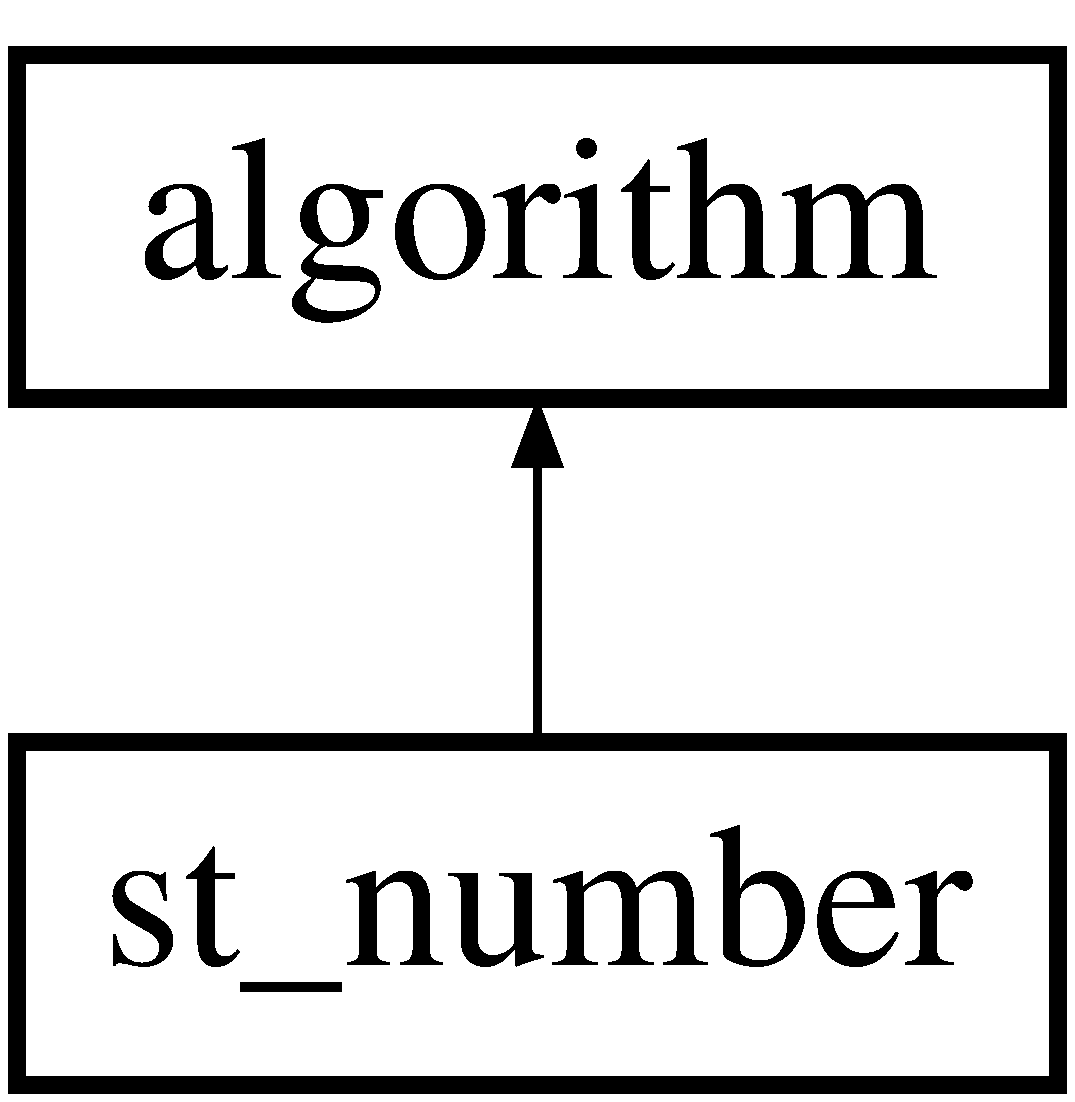
\includegraphics[height=2.000000cm]{classst__number}
\end{center}
\end{figure}
\subsection*{Public Types}
\begin{DoxyCompactItemize}
\item 
\mbox{\Hypertarget{classst__number_aaed068377f71f1901942f623086c6106}\label{classst__number_aaed068377f71f1901942f623086c6106}} 
typedef list$<$ \mbox{\hyperlink{classnode}{node}} $>$\+::iterator {\bfseries iterator}
\item 
\mbox{\Hypertarget{classst__number_a2029accd27725f982c898b0220e625af}\label{classst__number_a2029accd27725f982c898b0220e625af}} 
typedef list$<$ \mbox{\hyperlink{classnode}{node}} $>$\+::reverse\+\_\+iterator {\bfseries reverse\+\_\+iterator}
\end{DoxyCompactItemize}
\subsection*{Public Member Functions}
\begin{DoxyCompactItemize}
\item 
\mbox{\Hypertarget{classst__number_a07532323fbcc643dfc419809385b64a7}\label{classst__number_a07532323fbcc643dfc419809385b64a7}} 
\mbox{\hyperlink{classst__number_a07532323fbcc643dfc419809385b64a7}{st\+\_\+number}} ()
\begin{DoxyCompactList}\small\item\em Default constructor. Creates st-\/number object. Please note that there are no reasonable default settings for the parameters, i.\+e. the edge  st connecting the lowest with highest numbers node and which of its endpoints should get number 1 (= node {\itshape s}) has to be specified always. \end{DoxyCompactList}\item 
\mbox{\Hypertarget{classst__number_a4f3a2a6ceab39d106c920ee3546c259d}\label{classst__number_a4f3a2a6ceab39d106c920ee3546c259d}} 
virtual \mbox{\hyperlink{classst__number_a4f3a2a6ceab39d106c920ee3546c259d}{$\sim$st\+\_\+number}} ()
\begin{DoxyCompactList}\small\item\em Destructor. \end{DoxyCompactList}\item 
void \mbox{\hyperlink{classst__number_a1564af6f603160105643f22bf2f6955b}{st\+\_\+edge}} (\mbox{\hyperlink{classedge}{edge}} e)
\begin{DoxyCompactList}\small\item\em Sets edge {\itshape st} for the next run. \end{DoxyCompactList}\item 
\mbox{\hyperlink{classedge}{edge}} \mbox{\hyperlink{classst__number_a8938bab7883ff4194d1a7b4c6d8fb471}{st\+\_\+edge}} () const
\begin{DoxyCompactList}\small\item\em Get edge {\itshape st}. \end{DoxyCompactList}\item 
void \mbox{\hyperlink{classst__number_aa607c9aaa5a4d9c45e5854ce672f0fda}{s\+\_\+node}} (\mbox{\hyperlink{classnode}{node}} n)
\begin{DoxyCompactList}\small\item\em Sets node {\itshape s} for next run. \end{DoxyCompactList}\item 
\mbox{\hyperlink{classnode}{node}} \mbox{\hyperlink{classst__number_aba061fba83eb63b7a23dd685e1db663c}{s\+\_\+node}} () const
\begin{DoxyCompactList}\small\item\em Get node {\itshape s}. \end{DoxyCompactList}\item 
int \& \mbox{\hyperlink{classst__number_a969162a10da5daba4219419d45c4be51}{operator\mbox{[}$\,$\mbox{]}}} (const \mbox{\hyperlink{classnode}{node}} \&n)
\begin{DoxyCompactList}\small\item\em Returns st-\/number of node {\ttfamily n} as determined in the last run. \end{DoxyCompactList}\item 
iterator \mbox{\hyperlink{classst__number_a1eddb2577b16109d22cde98a8ffde057}{begin}} ()
\begin{DoxyCompactList}\small\item\em Iteration through the nodes of graph st-\/numbered in last run in st-\/number order, i.\+e. from 1 to highest st-\/number. \end{DoxyCompactList}\item 
iterator \mbox{\hyperlink{classst__number_a3912b83a8cbddcb1fc804d20be528d52}{end}} ()
\begin{DoxyCompactList}\small\item\em Iteration through nodes of graph in st-\/number order. \end{DoxyCompactList}\item 
reverse\+\_\+iterator \mbox{\hyperlink{classst__number_a56f2c67e9b49362947fe0c99278f6d31}{rbegin}} ()
\begin{DoxyCompactList}\small\item\em Iteration through the nodes of graph st-\/numbered in last run in reverse st-\/number order, i.\+e. from highest st-\/number down to 1. \end{DoxyCompactList}\item 
reverse\+\_\+iterator \mbox{\hyperlink{classst__number_a4c5fdce6ab2be7ee9ddbb09e8d5c8560}{rend}} ()
\begin{DoxyCompactList}\small\item\em End of iteration through nodes of graph in reverse st-\/number order. \end{DoxyCompactList}\item 
int \mbox{\hyperlink{classst__number_a2aad4550b821c52d6998bff35fd8648f}{check}} (\mbox{\hyperlink{classgraph}{graph}} \&G)
\begin{DoxyCompactList}\small\item\em Checks whether st-\/number algorithm can be applied to {\ttfamily G}. \end{DoxyCompactList}\item 
int \mbox{\hyperlink{classst__number_af902a0c05d07d47b587e8f7a6b7beaa1}{run}} (\mbox{\hyperlink{classgraph}{graph}} \&G)
\begin{DoxyCompactList}\small\item\em Runs st-\/number algorithm on graph {\ttfamily G}. \end{DoxyCompactList}\item 
void \mbox{\hyperlink{classst__number_ae6f86706b8ae3495d3794b8c684fff0f}{reset}} ()
\begin{DoxyCompactList}\small\item\em Resets algorithm in order to be applied to the next graph. \end{DoxyCompactList}\end{DoxyCompactItemize}
\subsection*{Protected Attributes}
\begin{DoxyCompactItemize}
\item 
\mbox{\Hypertarget{classst__number_a58fe3a128f0d06ce17742b62d8eff1a8}\label{classst__number_a58fe3a128f0d06ce17742b62d8eff1a8}} 
\mbox{\hyperlink{classedge}{edge}} {\bfseries st}
\item 
\mbox{\Hypertarget{classst__number_a1ada73c04f88b70b2392aa9ab0d1a6b0}\label{classst__number_a1ada73c04f88b70b2392aa9ab0d1a6b0}} 
\mbox{\hyperlink{classnode}{node}} {\bfseries s}
\item 
\mbox{\Hypertarget{classst__number_a2aa9c83b684379d86c4e620f0a3e5703}\label{classst__number_a2aa9c83b684379d86c4e620f0a3e5703}} 
\mbox{\hyperlink{classpathfinder}{pathfinder}} $\ast$ {\bfseries pf}
\item 
\mbox{\Hypertarget{classst__number_a01e08e56e7251800233b16eb6140c156}\label{classst__number_a01e08e56e7251800233b16eb6140c156}} 
list$<$ \mbox{\hyperlink{classnode}{node}} $>$ {\bfseries st\+\_\+ord}
\item 
\mbox{\Hypertarget{classst__number_ac3443aa6c9d11b990357d8ac1342cabc}\label{classst__number_ac3443aa6c9d11b990357d8ac1342cabc}} 
\mbox{\hyperlink{classnode__map}{node\+\_\+map}}$<$ int $>$ {\bfseries st\+\_\+num}
\end{DoxyCompactItemize}


\subsection{Detailed Description}
S\+T-\/number algorithm. 

Encapsulates the st-\/number algorithm together with all the data produced by it. 

Assigns an integer {\ttfamily st\mbox{[}n\mbox{]}} to each node {\ttfamily n} of a undirected, biconnected graph, such that each node is connected with at least one node having a smaller and with at least one having a larger number than itself. The only exception to this rule are the endpoints of edge {\itshape st} connecting nodes {\itshape s} (st-\/number 1) and {\ttfamily t} (highest st-\/number). 

The following options are supported\+:
\begin{DoxyItemize}
\item \mbox{\hyperlink{classst__number_a1564af6f603160105643f22bf2f6955b}{st\+\_\+edge}} sets/retrieves the edge that connects the node with the lowest number to that with the highest.
\item \mbox{\hyperlink{classst__number_aa607c9aaa5a4d9c45e5854ce672f0fda}{s\+\_\+node}} sets/retrieves that endpoints of the {\itshape st\+\_\+edge}, which gets number 1. 
\end{DoxyItemize}

\subsection{Member Function Documentation}
\mbox{\Hypertarget{classst__number_a1eddb2577b16109d22cde98a8ffde057}\label{classst__number_a1eddb2577b16109d22cde98a8ffde057}} 
\index{st\+\_\+number@{st\+\_\+number}!begin@{begin}}
\index{begin@{begin}!st\+\_\+number@{st\+\_\+number}}
\subsubsection{\texorpdfstring{begin()}{begin()}}
{\footnotesize\ttfamily iterator st\+\_\+number\+::begin (\begin{DoxyParamCaption}{ }\end{DoxyParamCaption})\hspace{0.3cm}{\ttfamily [inline]}}



Iteration through the nodes of graph st-\/numbered in last run in st-\/number order, i.\+e. from 1 to highest st-\/number. 

\begin{DoxyReturn}{Returns}
start of iteration through nodes in st-\/number order 
\end{DoxyReturn}
\mbox{\Hypertarget{classst__number_a2aad4550b821c52d6998bff35fd8648f}\label{classst__number_a2aad4550b821c52d6998bff35fd8648f}} 
\index{st\+\_\+number@{st\+\_\+number}!check@{check}}
\index{check@{check}!st\+\_\+number@{st\+\_\+number}}
\subsubsection{\texorpdfstring{check()}{check()}}
{\footnotesize\ttfamily int st\+\_\+number\+::check (\begin{DoxyParamCaption}\item[{\mbox{\hyperlink{classgraph}{graph}} \&}]{G }\end{DoxyParamCaption})\hspace{0.3cm}{\ttfamily [virtual]}}



Checks whether st-\/number algorithm can be applied to {\ttfamily G}. 

Besides from the trivial preconditions that edge {\itshape st} and node {\itshape s} lie in {\ttfamily G} and {\itshape s} is really an endpoint of {\itshape st} (which isn\textquotesingle{}t checked), {\ttfamily G} must be undirected and biconnected. \begin{DoxyNote}{Note}
As for all algorithms in K\+G\+L\+\_\+, \mbox{\hyperlink{classst__number_a2aad4550b821c52d6998bff35fd8648f}{check}} must be called, because it might do some initialization.
\end{DoxyNote}

\begin{DoxyParams}{Parameters}
{\em G} & graph\\
\hline
\end{DoxyParams}

\begin{DoxyRetVals}{Return values}
{\em \mbox{\hyperlink{classalgorithm_af1a0078e153aa99c24f9bdf0d97f6710aae4c1cd7fe8d8cf4b143241a6e7c31cf}{algorithm\+::\+K\+G\+L\+\_\+\+OK}}} & iff st-\/number algorithm may be applied\\
\hline
\end{DoxyRetVals}
\begin{DoxySeeAlso}{See also}
\mbox{\hyperlink{classalgorithm_a76361fb03ad1cf643affc51821e43bed}{algorithm\+::check}} 
\end{DoxySeeAlso}


Implements \mbox{\hyperlink{classalgorithm_a76361fb03ad1cf643affc51821e43bed}{algorithm}}.

\mbox{\Hypertarget{classst__number_a3912b83a8cbddcb1fc804d20be528d52}\label{classst__number_a3912b83a8cbddcb1fc804d20be528d52}} 
\index{st\+\_\+number@{st\+\_\+number}!end@{end}}
\index{end@{end}!st\+\_\+number@{st\+\_\+number}}
\subsubsection{\texorpdfstring{end()}{end()}}
{\footnotesize\ttfamily iterator st\+\_\+number\+::end (\begin{DoxyParamCaption}{ }\end{DoxyParamCaption})\hspace{0.3cm}{\ttfamily [inline]}}



Iteration through nodes of graph in st-\/number order. 

\begin{DoxyReturn}{Returns}
end of iteration through nodes of graph in st-\/number order 
\end{DoxyReturn}
\mbox{\Hypertarget{classst__number_a969162a10da5daba4219419d45c4be51}\label{classst__number_a969162a10da5daba4219419d45c4be51}} 
\index{st\+\_\+number@{st\+\_\+number}!operator\mbox{[}\mbox{]}@{operator[]}}
\index{operator\mbox{[}\mbox{]}@{operator[]}!st\+\_\+number@{st\+\_\+number}}
\subsubsection{\texorpdfstring{operator[]()}{operator[]()}}
{\footnotesize\ttfamily int\& st\+\_\+number\+::operator\mbox{[}$\,$\mbox{]} (\begin{DoxyParamCaption}\item[{const \mbox{\hyperlink{classnode}{node}} \&}]{n }\end{DoxyParamCaption})\hspace{0.3cm}{\ttfamily [inline]}}



Returns st-\/number of node {\ttfamily n} as determined in the last run. 


\begin{DoxyParams}{Parameters}
{\em n} & node\\
\hline
\end{DoxyParams}
\begin{DoxyReturn}{Returns}
st-\/number of {\ttfamily n} 
\end{DoxyReturn}
\mbox{\Hypertarget{classst__number_a56f2c67e9b49362947fe0c99278f6d31}\label{classst__number_a56f2c67e9b49362947fe0c99278f6d31}} 
\index{st\+\_\+number@{st\+\_\+number}!rbegin@{rbegin}}
\index{rbegin@{rbegin}!st\+\_\+number@{st\+\_\+number}}
\subsubsection{\texorpdfstring{rbegin()}{rbegin()}}
{\footnotesize\ttfamily reverse\+\_\+iterator st\+\_\+number\+::rbegin (\begin{DoxyParamCaption}{ }\end{DoxyParamCaption})\hspace{0.3cm}{\ttfamily [inline]}}



Iteration through the nodes of graph st-\/numbered in last run in reverse st-\/number order, i.\+e. from highest st-\/number down to 1. 

\begin{DoxyReturn}{Returns}
start of iteration through nodes in reverse st-\/number order 
\end{DoxyReturn}
\mbox{\Hypertarget{classst__number_a4c5fdce6ab2be7ee9ddbb09e8d5c8560}\label{classst__number_a4c5fdce6ab2be7ee9ddbb09e8d5c8560}} 
\index{st\+\_\+number@{st\+\_\+number}!rend@{rend}}
\index{rend@{rend}!st\+\_\+number@{st\+\_\+number}}
\subsubsection{\texorpdfstring{rend()}{rend()}}
{\footnotesize\ttfamily reverse\+\_\+iterator st\+\_\+number\+::rend (\begin{DoxyParamCaption}{ }\end{DoxyParamCaption})\hspace{0.3cm}{\ttfamily [inline]}}



End of iteration through nodes of graph in reverse st-\/number order. 

\begin{DoxyReturn}{Returns}
end of iteration through nodes in reverse st-\/number order 
\end{DoxyReturn}
\mbox{\Hypertarget{classst__number_ae6f86706b8ae3495d3794b8c684fff0f}\label{classst__number_ae6f86706b8ae3495d3794b8c684fff0f}} 
\index{st\+\_\+number@{st\+\_\+number}!reset@{reset}}
\index{reset@{reset}!st\+\_\+number@{st\+\_\+number}}
\subsubsection{\texorpdfstring{reset()}{reset()}}
{\footnotesize\ttfamily void st\+\_\+number\+::reset (\begin{DoxyParamCaption}{ }\end{DoxyParamCaption})\hspace{0.3cm}{\ttfamily [inline]}, {\ttfamily [virtual]}}



Resets algorithm in order to be applied to the next graph. 

This will delete most of the information obtained in the last run.

\begin{DoxySeeAlso}{See also}
\mbox{\hyperlink{classalgorithm_a21aba63d066ae7897de6ca7d8425c408}{algorithm\+::reset}} 
\end{DoxySeeAlso}


Implements \mbox{\hyperlink{classalgorithm_a21aba63d066ae7897de6ca7d8425c408}{algorithm}}.

\mbox{\Hypertarget{classst__number_af902a0c05d07d47b587e8f7a6b7beaa1}\label{classst__number_af902a0c05d07d47b587e8f7a6b7beaa1}} 
\index{st\+\_\+number@{st\+\_\+number}!run@{run}}
\index{run@{run}!st\+\_\+number@{st\+\_\+number}}
\subsubsection{\texorpdfstring{run()}{run()}}
{\footnotesize\ttfamily int st\+\_\+number\+::run (\begin{DoxyParamCaption}\item[{\mbox{\hyperlink{classgraph}{graph}} \&}]{G }\end{DoxyParamCaption})\hspace{0.3cm}{\ttfamily [virtual]}}



Runs st-\/number algorithm on graph {\ttfamily G}. 

It is assumed that \mbox{\hyperlink{classst__number_a2aad4550b821c52d6998bff35fd8648f}{check}} was called previously and returned \mbox{\hyperlink{classalgorithm_af1a0078e153aa99c24f9bdf0d97f6710aae4c1cd7fe8d8cf4b143241a6e7c31cf}{algorithm\+::\+K\+G\+L\+\_\+\+OK}}.


\begin{DoxyParams}{Parameters}
{\em G} & graph\\
\hline
\end{DoxyParams}
\begin{DoxyReturn}{Returns}
\mbox{\hyperlink{classalgorithm_af1a0078e153aa99c24f9bdf0d97f6710aae4c1cd7fe8d8cf4b143241a6e7c31cf}{algorithm\+::\+K\+G\+L\+\_\+\+OK}} iff {\ttfamily G} could be correctly st-\/numbered
\end{DoxyReturn}
\begin{DoxySeeAlso}{See also}
\mbox{\hyperlink{classalgorithm_a734b189509a8d6b56b65f8ff772d43ca}{algorithm\+::run}} 
\end{DoxySeeAlso}


Implements \mbox{\hyperlink{classalgorithm_a734b189509a8d6b56b65f8ff772d43ca}{algorithm}}.

\mbox{\Hypertarget{classst__number_aa607c9aaa5a4d9c45e5854ce672f0fda}\label{classst__number_aa607c9aaa5a4d9c45e5854ce672f0fda}} 
\index{st\+\_\+number@{st\+\_\+number}!s\+\_\+node@{s\+\_\+node}}
\index{s\+\_\+node@{s\+\_\+node}!st\+\_\+number@{st\+\_\+number}}
\subsubsection{\texorpdfstring{s\+\_\+node()}{s\_node()}\hspace{0.1cm}{\footnotesize\ttfamily [1/2]}}
{\footnotesize\ttfamily void st\+\_\+number\+::s\+\_\+node (\begin{DoxyParamCaption}\item[{\mbox{\hyperlink{classnode}{node}}}]{n }\end{DoxyParamCaption})\hspace{0.3cm}{\ttfamily [inline]}}



Sets node {\itshape s} for next run. 

This must be one of the endpoints of edge {\itshape st}. This node will get st-\/number 1 and thus the other endpoint will get the highest st-\/number.


\begin{DoxyParams}{Parameters}
{\em n} & node {\itshape s} \\
\hline
\end{DoxyParams}
\mbox{\Hypertarget{classst__number_aba061fba83eb63b7a23dd685e1db663c}\label{classst__number_aba061fba83eb63b7a23dd685e1db663c}} 
\index{st\+\_\+number@{st\+\_\+number}!s\+\_\+node@{s\+\_\+node}}
\index{s\+\_\+node@{s\+\_\+node}!st\+\_\+number@{st\+\_\+number}}
\subsubsection{\texorpdfstring{s\+\_\+node()}{s\_node()}\hspace{0.1cm}{\footnotesize\ttfamily [2/2]}}
{\footnotesize\ttfamily \mbox{\hyperlink{classnode}{node}} st\+\_\+number\+::s\+\_\+node (\begin{DoxyParamCaption}{ }\end{DoxyParamCaption}) const\hspace{0.3cm}{\ttfamily [inline]}}



Get node {\itshape s}. 


\begin{DoxyRetVals}{Return values}
{\em node} & {\itshape s} \\
\hline
\end{DoxyRetVals}
\mbox{\Hypertarget{classst__number_a1564af6f603160105643f22bf2f6955b}\label{classst__number_a1564af6f603160105643f22bf2f6955b}} 
\index{st\+\_\+number@{st\+\_\+number}!st\+\_\+edge@{st\+\_\+edge}}
\index{st\+\_\+edge@{st\+\_\+edge}!st\+\_\+number@{st\+\_\+number}}
\subsubsection{\texorpdfstring{st\+\_\+edge()}{st\_edge()}\hspace{0.1cm}{\footnotesize\ttfamily [1/2]}}
{\footnotesize\ttfamily void st\+\_\+number\+::st\+\_\+edge (\begin{DoxyParamCaption}\item[{\mbox{\hyperlink{classedge}{edge}}}]{e }\end{DoxyParamCaption})\hspace{0.3cm}{\ttfamily [inline]}}



Sets edge {\itshape st} for the next run. 


\begin{DoxyParams}{Parameters}
{\em e} & edge {\itshape st} \\
\hline
\end{DoxyParams}
\mbox{\Hypertarget{classst__number_a8938bab7883ff4194d1a7b4c6d8fb471}\label{classst__number_a8938bab7883ff4194d1a7b4c6d8fb471}} 
\index{st\+\_\+number@{st\+\_\+number}!st\+\_\+edge@{st\+\_\+edge}}
\index{st\+\_\+edge@{st\+\_\+edge}!st\+\_\+number@{st\+\_\+number}}
\subsubsection{\texorpdfstring{st\+\_\+edge()}{st\_edge()}\hspace{0.1cm}{\footnotesize\ttfamily [2/2]}}
{\footnotesize\ttfamily \mbox{\hyperlink{classedge}{edge}} st\+\_\+number\+::st\+\_\+edge (\begin{DoxyParamCaption}{ }\end{DoxyParamCaption}) const\hspace{0.3cm}{\ttfamily [inline]}}



Get edge {\itshape st}. 


\begin{DoxyRetVals}{Return values}
{\em edge} & {\itshape st} \\
\hline
\end{DoxyRetVals}


The documentation for this class was generated from the following files\+:\begin{DoxyCompactItemize}
\item 
include/\+K\+G\+L/st\+\_\+number.\+h\item 
src/st\+\_\+number.\+cpp\end{DoxyCompactItemize}

\hypertarget{classsymlist}{}\section{symlist$<$ T $>$ Class Template Reference}
\label{classsymlist}\index{symlist$<$ T $>$@{symlist$<$ T $>$}}


List which can be reversed in $\mathcal{O}(1)$.  




{\ttfamily \#include $<$symlist.\+h$>$}

\subsection*{Public Types}
\begin{DoxyCompactItemize}
\item 
\mbox{\Hypertarget{classsymlist_a66045fbe3d98975e5537092ede8b50df}\label{classsymlist_a66045fbe3d98975e5537092ede8b50df}} 
typedef \mbox{\hyperlink{structsymlist__iterator}{symlist\+\_\+iterator}}$<$ T, T \& $>$ {\bfseries iterator}
\item 
\mbox{\Hypertarget{classsymlist_af15c0ca931299054f83d17a1580a5159}\label{classsymlist_af15c0ca931299054f83d17a1580a5159}} 
typedef \mbox{\hyperlink{structsymlist__iterator}{symlist\+\_\+iterator}}$<$ T, const T \& $>$ {\bfseries const\+\_\+iterator}
\end{DoxyCompactItemize}
\subsection*{Public Member Functions}
\begin{DoxyCompactItemize}
\item 
\mbox{\Hypertarget{classsymlist_a678dc0ddb02994195a2359a361ee0ea6}\label{classsymlist_a678dc0ddb02994195a2359a361ee0ea6}} 
\mbox{\hyperlink{classsymlist_a678dc0ddb02994195a2359a361ee0ea6}{symlist}} ()
\begin{DoxyCompactList}\small\item\em Creates empty symlist. \end{DoxyCompactList}\item 
\mbox{\hyperlink{classsymlist_a5c17d54592dac03b2c4d940a10153797}{symlist}} (const \mbox{\hyperlink{classsymlist}{symlist}}$<$ T $>$ \&li)
\begin{DoxyCompactList}\small\item\em Makes the created list a copy of {\ttfamily li}. \end{DoxyCompactList}\item 
\mbox{\hyperlink{classsymlist}{symlist}}$<$ T $>$ \& \mbox{\hyperlink{classsymlist_aab326eda0f6d3a78f193a249342670bc}{operator=}} (const \mbox{\hyperlink{classsymlist}{symlist}}$<$ T $>$ \&li)
\begin{DoxyCompactList}\small\item\em Assignes {\ttfamily li} to this list. \end{DoxyCompactList}\item 
\mbox{\Hypertarget{classsymlist_a45c3a0b7f0e996998037fb876effefd4}\label{classsymlist_a45c3a0b7f0e996998037fb876effefd4}} 
\mbox{\hyperlink{classsymlist_a45c3a0b7f0e996998037fb876effefd4}{$\sim$symlist}} ()
\begin{DoxyCompactList}\small\item\em Destructor. \end{DoxyCompactList}\item 
bool \mbox{\hyperlink{classsymlist_aca11cd6c621376bc52a18828ef92e753}{empty}} () const
\begin{DoxyCompactList}\small\item\em Checks whether list is empty. \end{DoxyCompactList}\item 
T \& \mbox{\hyperlink{classsymlist_afd4b55616fc20033d4a47684551866e8}{front}} ()
\begin{DoxyCompactList}\small\item\em First element in list. \end{DoxyCompactList}\item 
T \& \mbox{\hyperlink{classsymlist_abc0570ff78ded9210ac26865519d36e3}{back}} ()
\begin{DoxyCompactList}\small\item\em Last element in list. \end{DoxyCompactList}\item 
\mbox{\hyperlink{structsymlist__iterator}{iterator}} \mbox{\hyperlink{classsymlist_a525b8d44af5d771fe15916372515cce0}{begin}} ()
\begin{DoxyCompactList}\small\item\em Start iteration through elements of list. \end{DoxyCompactList}\item 
\mbox{\hyperlink{structsymlist__iterator}{iterator}} \mbox{\hyperlink{classsymlist_a7283589fa01f79d722f8256d7a6a7883}{end}} ()
\begin{DoxyCompactList}\small\item\em End of iteration through elements of list. \end{DoxyCompactList}\item 
\mbox{\hyperlink{structsymlist__iterator}{const\+\_\+iterator}} \mbox{\hyperlink{classsymlist_a843d2df09f34079f6547f338b50823cd}{begin}} () const
\begin{DoxyCompactList}\small\item\em Start iteration through elements of list. \end{DoxyCompactList}\item 
\mbox{\hyperlink{structsymlist__iterator}{const\+\_\+iterator}} \mbox{\hyperlink{classsymlist_a189c41a13b3dd377c113d802258ef418}{end}} () const
\begin{DoxyCompactList}\small\item\em End of iteration through elements of list. \end{DoxyCompactList}\item 
\mbox{\hyperlink{structsymlist__iterator}{iterator}} \mbox{\hyperlink{classsymlist_ae5250e0c0c2bedee285f72584ddce29d}{rbegin}} ()
\begin{DoxyCompactList}\small\item\em Start iteration through element of list in reverse order. \end{DoxyCompactList}\item 
\mbox{\hyperlink{structsymlist__iterator}{iterator}} \mbox{\hyperlink{classsymlist_a421fc482e62f257a9081e9e1c29d66a6}{rend}} ()
\begin{DoxyCompactList}\small\item\em End of iteration through elements of list in reverse order. \end{DoxyCompactList}\item 
\mbox{\hyperlink{structsymlist__iterator}{const\+\_\+iterator}} \mbox{\hyperlink{classsymlist_a3779415d5588f9621494f40789841caf}{rbegin}} () const
\begin{DoxyCompactList}\small\item\em Start iteration through element of list in reverse order. \end{DoxyCompactList}\item 
\mbox{\hyperlink{structsymlist__iterator}{const\+\_\+iterator}} \mbox{\hyperlink{classsymlist_a42379ebaa07ddb1160d785fec701712d}{rend}} () const
\begin{DoxyCompactList}\small\item\em End of iteration through elements of list in reverse order. \end{DoxyCompactList}\item 
\mbox{\hyperlink{structsymlist__iterator}{iterator}} \mbox{\hyperlink{classsymlist_a8b3327b8a33b180bf1eb802856f755c3}{insert}} (\mbox{\hyperlink{structsymlist__iterator}{iterator}} pos, const T \&data)
\begin{DoxyCompactList}\small\item\em Inserts {\ttfamily data} before {\ttfamily pos} in list. \end{DoxyCompactList}\item 
void \mbox{\hyperlink{classsymlist_ac2bd4d9db62ea6a3282662c62a97c3b2}{splice}} (\mbox{\hyperlink{structsymlist__iterator}{iterator}} pos, \mbox{\hyperlink{structsymlist__iterator}{iterator}} it)
\begin{DoxyCompactList}\small\item\em Inserts the element {\ttfamily it} points to before {\ttfamily pos} into this list. \end{DoxyCompactList}\item 
void \mbox{\hyperlink{classsymlist_a27889c85e97c1e8dec7a871987a12b29}{splice}} (\mbox{\hyperlink{structsymlist__iterator}{iterator}} pos, \mbox{\hyperlink{structsymlist__iterator}{iterator}} it, \mbox{\hyperlink{structsymlist__iterator}{iterator}} \mbox{\hyperlink{classsymlist_a7283589fa01f79d722f8256d7a6a7883}{end}})
\begin{DoxyCompactList}\small\item\em Inserts the elements {\ttfamily \mbox{[}it,end)} refers to before {\ttfamily pos} into this list. \end{DoxyCompactList}\item 
\mbox{\hyperlink{structsymlist__iterator}{iterator}} \mbox{\hyperlink{classsymlist_a75fc1fc7db7b20cc430ddb8577608904}{erase}} (\mbox{\hyperlink{structsymlist__iterator}{iterator}} pos)
\begin{DoxyCompactList}\small\item\em Deletes element at position {\ttfamily pos} from list. \end{DoxyCompactList}\item 
\mbox{\hyperlink{structsymlist__iterator}{iterator}} \mbox{\hyperlink{classsymlist_a53128defa9aedb016affcfa27bf201da}{erase}} (\mbox{\hyperlink{structsymlist__iterator}{iterator}} it, \mbox{\hyperlink{structsymlist__iterator}{iterator}} \mbox{\hyperlink{classsymlist_a7283589fa01f79d722f8256d7a6a7883}{end}})
\begin{DoxyCompactList}\small\item\em Deletes the elements {\ttfamily \mbox{[}it, end)} from list. \end{DoxyCompactList}\item 
\mbox{\Hypertarget{classsymlist_a526206a1d6fd2f2cef9f73ec499b6315}\label{classsymlist_a526206a1d6fd2f2cef9f73ec499b6315}} 
void {\bfseries attach\+\_\+sublist} (\mbox{\hyperlink{structsymlist__iterator}{iterator}}, \mbox{\hyperlink{structsymlist__iterator}{iterator}})
\item 
\mbox{\Hypertarget{classsymlist_a784f81bf9dfbfc1865f188a82681779f}\label{classsymlist_a784f81bf9dfbfc1865f188a82681779f}} 
void {\bfseries detach\+\_\+sublist} ()
\item 
void \mbox{\hyperlink{classsymlist_ae22b65101604c694e96974cc9579ab78}{reverse}} ()
\begin{DoxyCompactList}\small\item\em Change the direction of list. \end{DoxyCompactList}\end{DoxyCompactItemize}


\subsection{Detailed Description}
\subsubsection*{template$<$class T$>$\newline
class symlist$<$ T $>$}

List which can be reversed in $\mathcal{O}(1)$. 

The problem with the S\+TL class list -\/ as with most doubly linked lists -- is that isn\textquotesingle{}t possible to turn it in constant time, because each entry in the list contains next and prev pointer and turning the list means to switch these two in {\itshape each} element in the list. Another point is the splice operation in S\+TL lists, which is constant time, but for the same reason as mentioned above it is not possible to splice a list in reverse order into another in constant time. 

The problems arise from the fact that each element \char`\"{}knows\char`\"{} what its next and previous elements are. An element in a symlist only knows what its neighbors are, what is next and what previous depends on the direction of iteration. This of course imposes some overhead in iteration (one if-\/statement) but allows reversion and a splice in reversed order in constant time. 

\subsection{Constructor \& Destructor Documentation}
\mbox{\Hypertarget{classsymlist_a5c17d54592dac03b2c4d940a10153797}\label{classsymlist_a5c17d54592dac03b2c4d940a10153797}} 
\index{symlist@{symlist}!symlist@{symlist}}
\index{symlist@{symlist}!symlist@{symlist}}
\subsubsection{\texorpdfstring{symlist()}{symlist()}}
{\footnotesize\ttfamily template$<$class T$>$ \\
\mbox{\hyperlink{classsymlist}{symlist}}$<$ T $>$\+::\mbox{\hyperlink{classsymlist}{symlist}} (\begin{DoxyParamCaption}\item[{const \mbox{\hyperlink{classsymlist}{symlist}}$<$ T $>$ \&}]{li }\end{DoxyParamCaption})}



Makes the created list a copy of {\ttfamily li}. 


\begin{DoxyParams}{Parameters}
{\em li} & symlist. \\
\hline
\end{DoxyParams}


\subsection{Member Function Documentation}
\mbox{\Hypertarget{classsymlist_abc0570ff78ded9210ac26865519d36e3}\label{classsymlist_abc0570ff78ded9210ac26865519d36e3}} 
\index{symlist@{symlist}!back@{back}}
\index{back@{back}!symlist@{symlist}}
\subsubsection{\texorpdfstring{back()}{back()}}
{\footnotesize\ttfamily template$<$class T$>$ \\
T\& \mbox{\hyperlink{classsymlist}{symlist}}$<$ T $>$\+::back (\begin{DoxyParamCaption}{ }\end{DoxyParamCaption})\hspace{0.3cm}{\ttfamily [inline]}}



Last element in list. 

Assumes that list ins\textquotesingle{}t empty.

\begin{DoxyReturn}{Returns}
last element 
\end{DoxyReturn}
\mbox{\Hypertarget{classsymlist_a525b8d44af5d771fe15916372515cce0}\label{classsymlist_a525b8d44af5d771fe15916372515cce0}} 
\index{symlist@{symlist}!begin@{begin}}
\index{begin@{begin}!symlist@{symlist}}
\subsubsection{\texorpdfstring{begin()}{begin()}\hspace{0.1cm}{\footnotesize\ttfamily [1/2]}}
{\footnotesize\ttfamily template$<$class T$>$ \\
\mbox{\hyperlink{structsymlist__iterator}{iterator}} \mbox{\hyperlink{classsymlist}{symlist}}$<$ T $>$\+::begin (\begin{DoxyParamCaption}{ }\end{DoxyParamCaption})\hspace{0.3cm}{\ttfamily [inline]}}



Start iteration through elements of list. 

\begin{DoxyReturn}{Returns}
start iterator 
\end{DoxyReturn}
\mbox{\Hypertarget{classsymlist_a843d2df09f34079f6547f338b50823cd}\label{classsymlist_a843d2df09f34079f6547f338b50823cd}} 
\index{symlist@{symlist}!begin@{begin}}
\index{begin@{begin}!symlist@{symlist}}
\subsubsection{\texorpdfstring{begin()}{begin()}\hspace{0.1cm}{\footnotesize\ttfamily [2/2]}}
{\footnotesize\ttfamily template$<$class T$>$ \\
\mbox{\hyperlink{structsymlist__iterator}{const\+\_\+iterator}} \mbox{\hyperlink{classsymlist}{symlist}}$<$ T $>$\+::begin (\begin{DoxyParamCaption}{ }\end{DoxyParamCaption}) const\hspace{0.3cm}{\ttfamily [inline]}}



Start iteration through elements of list. 

\begin{DoxyReturn}{Returns}
start iterator 
\end{DoxyReturn}
\mbox{\Hypertarget{classsymlist_aca11cd6c621376bc52a18828ef92e753}\label{classsymlist_aca11cd6c621376bc52a18828ef92e753}} 
\index{symlist@{symlist}!empty@{empty}}
\index{empty@{empty}!symlist@{symlist}}
\subsubsection{\texorpdfstring{empty()}{empty()}}
{\footnotesize\ttfamily template$<$class T$>$ \\
bool \mbox{\hyperlink{classsymlist}{symlist}}$<$ T $>$\+::empty (\begin{DoxyParamCaption}{ }\end{DoxyParamCaption}) const\hspace{0.3cm}{\ttfamily [inline]}}



Checks whether list is empty. 

Takes constant time.


\begin{DoxyRetVals}{Return values}
{\em true} & iff list is empty \\
\hline
\end{DoxyRetVals}
\mbox{\Hypertarget{classsymlist_a7283589fa01f79d722f8256d7a6a7883}\label{classsymlist_a7283589fa01f79d722f8256d7a6a7883}} 
\index{symlist@{symlist}!end@{end}}
\index{end@{end}!symlist@{symlist}}
\subsubsection{\texorpdfstring{end()}{end()}\hspace{0.1cm}{\footnotesize\ttfamily [1/2]}}
{\footnotesize\ttfamily template$<$class T$>$ \\
\mbox{\hyperlink{structsymlist__iterator}{iterator}} \mbox{\hyperlink{classsymlist}{symlist}}$<$ T $>$\+::end (\begin{DoxyParamCaption}{ }\end{DoxyParamCaption})\hspace{0.3cm}{\ttfamily [inline]}}



End of iteration through elements of list. 

\begin{DoxyReturn}{Returns}
end iterator 
\end{DoxyReturn}
\mbox{\Hypertarget{classsymlist_a189c41a13b3dd377c113d802258ef418}\label{classsymlist_a189c41a13b3dd377c113d802258ef418}} 
\index{symlist@{symlist}!end@{end}}
\index{end@{end}!symlist@{symlist}}
\subsubsection{\texorpdfstring{end()}{end()}\hspace{0.1cm}{\footnotesize\ttfamily [2/2]}}
{\footnotesize\ttfamily template$<$class T$>$ \\
\mbox{\hyperlink{structsymlist__iterator}{const\+\_\+iterator}} \mbox{\hyperlink{classsymlist}{symlist}}$<$ T $>$\+::end (\begin{DoxyParamCaption}{ }\end{DoxyParamCaption}) const\hspace{0.3cm}{\ttfamily [inline]}}



End of iteration through elements of list. 

\begin{DoxyReturn}{Returns}
end iterator 
\end{DoxyReturn}
\mbox{\Hypertarget{classsymlist_a75fc1fc7db7b20cc430ddb8577608904}\label{classsymlist_a75fc1fc7db7b20cc430ddb8577608904}} 
\index{symlist@{symlist}!erase@{erase}}
\index{erase@{erase}!symlist@{symlist}}
\subsubsection{\texorpdfstring{erase()}{erase()}\hspace{0.1cm}{\footnotesize\ttfamily [1/2]}}
{\footnotesize\ttfamily template$<$class T$>$ \\
\mbox{\hyperlink{structsymlist__iterator}{iterator}} \mbox{\hyperlink{classsymlist}{symlist}}$<$ T $>$\+::erase (\begin{DoxyParamCaption}\item[{\mbox{\hyperlink{structsymlist__iterator}{iterator}}}]{pos }\end{DoxyParamCaption})}



Deletes element at position {\ttfamily pos} from list. 


\begin{DoxyParams}{Parameters}
{\em pos} & position to be deleted\\
\hline
\end{DoxyParams}
\begin{DoxyReturn}{Returns}
position of next element 
\end{DoxyReturn}
\mbox{\Hypertarget{classsymlist_a53128defa9aedb016affcfa27bf201da}\label{classsymlist_a53128defa9aedb016affcfa27bf201da}} 
\index{symlist@{symlist}!erase@{erase}}
\index{erase@{erase}!symlist@{symlist}}
\subsubsection{\texorpdfstring{erase()}{erase()}\hspace{0.1cm}{\footnotesize\ttfamily [2/2]}}
{\footnotesize\ttfamily template$<$class T$>$ \\
\mbox{\hyperlink{structsymlist__iterator}{iterator}} \mbox{\hyperlink{classsymlist}{symlist}}$<$ T $>$\+::erase (\begin{DoxyParamCaption}\item[{\mbox{\hyperlink{structsymlist__iterator}{iterator}}}]{it,  }\item[{\mbox{\hyperlink{structsymlist__iterator}{iterator}}}]{end }\end{DoxyParamCaption})}



Deletes the elements {\ttfamily \mbox{[}it, end)} from list. 


\begin{DoxyParams}{Parameters}
{\em it} & first position to be deleted \\
\hline
{\em end} & one-\/past the last position to be deleted\\
\hline
\end{DoxyParams}
\begin{DoxyReturn}{Returns}
position of next element. 
\end{DoxyReturn}
\mbox{\Hypertarget{classsymlist_afd4b55616fc20033d4a47684551866e8}\label{classsymlist_afd4b55616fc20033d4a47684551866e8}} 
\index{symlist@{symlist}!front@{front}}
\index{front@{front}!symlist@{symlist}}
\subsubsection{\texorpdfstring{front()}{front()}}
{\footnotesize\ttfamily template$<$class T$>$ \\
T\& \mbox{\hyperlink{classsymlist}{symlist}}$<$ T $>$\+::front (\begin{DoxyParamCaption}{ }\end{DoxyParamCaption})\hspace{0.3cm}{\ttfamily [inline]}}



First element in list. 

Assumes that list ins\textquotesingle{}t empty.

\begin{DoxyReturn}{Returns}
first element 
\end{DoxyReturn}
\mbox{\Hypertarget{classsymlist_a8b3327b8a33b180bf1eb802856f755c3}\label{classsymlist_a8b3327b8a33b180bf1eb802856f755c3}} 
\index{symlist@{symlist}!insert@{insert}}
\index{insert@{insert}!symlist@{symlist}}
\subsubsection{\texorpdfstring{insert()}{insert()}}
{\footnotesize\ttfamily template$<$class T$>$ \\
\mbox{\hyperlink{structsymlist__iterator}{symlist\+\_\+iterator}}$<$ T, T \& $>$ \mbox{\hyperlink{classsymlist}{symlist}}$<$ T $>$\+::insert (\begin{DoxyParamCaption}\item[{\mbox{\hyperlink{structsymlist__iterator}{iterator}}}]{pos,  }\item[{const T \&}]{data }\end{DoxyParamCaption})}



Inserts {\ttfamily data} before {\ttfamily pos} in list. 


\begin{DoxyParams}{Parameters}
{\em pos} & position \\
\hline
{\em data} & element to be inserted\\
\hline
\end{DoxyParams}
\begin{DoxyReturn}{Returns}
position of insertion 
\end{DoxyReturn}
\mbox{\Hypertarget{classsymlist_aab326eda0f6d3a78f193a249342670bc}\label{classsymlist_aab326eda0f6d3a78f193a249342670bc}} 
\index{symlist@{symlist}!operator=@{operator=}}
\index{operator=@{operator=}!symlist@{symlist}}
\subsubsection{\texorpdfstring{operator=()}{operator=()}}
{\footnotesize\ttfamily template$<$class T$>$ \\
\mbox{\hyperlink{classsymlist}{symlist}}$<$ T $>$ \& \mbox{\hyperlink{classsymlist}{symlist}}$<$ T $>$\+::operator= (\begin{DoxyParamCaption}\item[{const \mbox{\hyperlink{classsymlist}{symlist}}$<$ T $>$ \&}]{li }\end{DoxyParamCaption})}



Assignes {\ttfamily li} to this list. 

\begin{DoxyNote}{Note}
All elements in this list will be deleted.
\end{DoxyNote}

\begin{DoxyParams}{Parameters}
{\em li} & \\
\hline
\end{DoxyParams}
\begin{DoxyReturn}{Returns}
this list 
\end{DoxyReturn}
\mbox{\Hypertarget{classsymlist_ae5250e0c0c2bedee285f72584ddce29d}\label{classsymlist_ae5250e0c0c2bedee285f72584ddce29d}} 
\index{symlist@{symlist}!rbegin@{rbegin}}
\index{rbegin@{rbegin}!symlist@{symlist}}
\subsubsection{\texorpdfstring{rbegin()}{rbegin()}\hspace{0.1cm}{\footnotesize\ttfamily [1/2]}}
{\footnotesize\ttfamily template$<$class T$>$ \\
\mbox{\hyperlink{structsymlist__iterator}{iterator}} \mbox{\hyperlink{classsymlist}{symlist}}$<$ T $>$\+::rbegin (\begin{DoxyParamCaption}{ }\end{DoxyParamCaption})\hspace{0.3cm}{\ttfamily [inline]}}



Start iteration through element of list in reverse order. 

\begin{DoxyReturn}{Returns}
start iterator 
\end{DoxyReturn}
\mbox{\Hypertarget{classsymlist_a3779415d5588f9621494f40789841caf}\label{classsymlist_a3779415d5588f9621494f40789841caf}} 
\index{symlist@{symlist}!rbegin@{rbegin}}
\index{rbegin@{rbegin}!symlist@{symlist}}
\subsubsection{\texorpdfstring{rbegin()}{rbegin()}\hspace{0.1cm}{\footnotesize\ttfamily [2/2]}}
{\footnotesize\ttfamily template$<$class T$>$ \\
\mbox{\hyperlink{structsymlist__iterator}{const\+\_\+iterator}} \mbox{\hyperlink{classsymlist}{symlist}}$<$ T $>$\+::rbegin (\begin{DoxyParamCaption}{ }\end{DoxyParamCaption}) const\hspace{0.3cm}{\ttfamily [inline]}}



Start iteration through element of list in reverse order. 

\begin{DoxyReturn}{Returns}
start iterator 
\end{DoxyReturn}
\mbox{\Hypertarget{classsymlist_a421fc482e62f257a9081e9e1c29d66a6}\label{classsymlist_a421fc482e62f257a9081e9e1c29d66a6}} 
\index{symlist@{symlist}!rend@{rend}}
\index{rend@{rend}!symlist@{symlist}}
\subsubsection{\texorpdfstring{rend()}{rend()}\hspace{0.1cm}{\footnotesize\ttfamily [1/2]}}
{\footnotesize\ttfamily template$<$class T$>$ \\
\mbox{\hyperlink{structsymlist__iterator}{iterator}} \mbox{\hyperlink{classsymlist}{symlist}}$<$ T $>$\+::rend (\begin{DoxyParamCaption}{ }\end{DoxyParamCaption})\hspace{0.3cm}{\ttfamily [inline]}}



End of iteration through elements of list in reverse order. 

\begin{DoxyReturn}{Returns}
end iterator 
\end{DoxyReturn}
\mbox{\Hypertarget{classsymlist_a42379ebaa07ddb1160d785fec701712d}\label{classsymlist_a42379ebaa07ddb1160d785fec701712d}} 
\index{symlist@{symlist}!rend@{rend}}
\index{rend@{rend}!symlist@{symlist}}
\subsubsection{\texorpdfstring{rend()}{rend()}\hspace{0.1cm}{\footnotesize\ttfamily [2/2]}}
{\footnotesize\ttfamily template$<$class T$>$ \\
\mbox{\hyperlink{structsymlist__iterator}{const\+\_\+iterator}} \mbox{\hyperlink{classsymlist}{symlist}}$<$ T $>$\+::rend (\begin{DoxyParamCaption}{ }\end{DoxyParamCaption}) const\hspace{0.3cm}{\ttfamily [inline]}}



End of iteration through elements of list in reverse order. 

\begin{DoxyReturn}{Returns}
end iterator 
\end{DoxyReturn}
\mbox{\Hypertarget{classsymlist_ae22b65101604c694e96974cc9579ab78}\label{classsymlist_ae22b65101604c694e96974cc9579ab78}} 
\index{symlist@{symlist}!reverse@{reverse}}
\index{reverse@{reverse}!symlist@{symlist}}
\subsubsection{\texorpdfstring{reverse()}{reverse()}}
{\footnotesize\ttfamily template$<$class T $>$ \\
void \mbox{\hyperlink{classsymlist}{symlist}}$<$ T $>$\+::reverse (\begin{DoxyParamCaption}{ }\end{DoxyParamCaption})\hspace{0.3cm}{\ttfamily [inline]}}



Change the direction of list. 

Takes constant time. \mbox{\Hypertarget{classsymlist_ac2bd4d9db62ea6a3282662c62a97c3b2}\label{classsymlist_ac2bd4d9db62ea6a3282662c62a97c3b2}} 
\index{symlist@{symlist}!splice@{splice}}
\index{splice@{splice}!symlist@{symlist}}
\subsubsection{\texorpdfstring{splice()}{splice()}\hspace{0.1cm}{\footnotesize\ttfamily [1/2]}}
{\footnotesize\ttfamily template$<$class T$>$ \\
void \mbox{\hyperlink{classsymlist}{symlist}}$<$ T $>$\+::splice (\begin{DoxyParamCaption}\item[{\mbox{\hyperlink{structsymlist__iterator}{iterator}}}]{pos,  }\item[{\mbox{\hyperlink{structsymlist__iterator}{iterator}}}]{it }\end{DoxyParamCaption})}



Inserts the element {\ttfamily it} points to before {\ttfamily pos} into this list. 

It is assumed that the element {\ttfamily it} refers lies in a different list. All iterators to elements in either of the two lists stay valid. Takes constant time.


\begin{DoxyParams}{Parameters}
{\em pos} & position \\
\hline
{\em it} & position of element to be inserted \\
\hline
\end{DoxyParams}
\mbox{\Hypertarget{classsymlist_a27889c85e97c1e8dec7a871987a12b29}\label{classsymlist_a27889c85e97c1e8dec7a871987a12b29}} 
\index{symlist@{symlist}!splice@{splice}}
\index{splice@{splice}!symlist@{symlist}}
\subsubsection{\texorpdfstring{splice()}{splice()}\hspace{0.1cm}{\footnotesize\ttfamily [2/2]}}
{\footnotesize\ttfamily template$<$class T$>$ \\
void \mbox{\hyperlink{classsymlist}{symlist}}$<$ T $>$\+::splice (\begin{DoxyParamCaption}\item[{\mbox{\hyperlink{structsymlist__iterator}{iterator}}}]{pos,  }\item[{\mbox{\hyperlink{structsymlist__iterator}{iterator}}}]{it,  }\item[{\mbox{\hyperlink{structsymlist__iterator}{iterator}}}]{end }\end{DoxyParamCaption})}



Inserts the elements {\ttfamily \mbox{[}it,end)} refers to before {\ttfamily pos} into this list. 

It is assumed that {\ttfamily \mbox{[}it,end)} lies in a different list. All iterators to elements in either of the two lists stay valid. Takes constant time.


\begin{DoxyParams}{Parameters}
{\em pos} & position \\
\hline
{\em it} & position of first element to be inserted \\
\hline
{\em end} & position of one-\/past the last element to be inserted \\
\hline
\end{DoxyParams}


The documentation for this class was generated from the following file\+:\begin{DoxyCompactItemize}
\item 
include/\+K\+G\+L/symlist.\+h\end{DoxyCompactItemize}

\hypertarget{structsymlist__iterator}{}\section{symlist\+\_\+iterator$<$ T, Ref $>$ Struct Template Reference}
\label{structsymlist__iterator}\index{symlist\+\_\+iterator$<$ T, Ref $>$@{symlist\+\_\+iterator$<$ T, Ref $>$}}
\subsection*{Public Types}
\begin{DoxyCompactItemize}
\item 
\mbox{\Hypertarget{structsymlist__iterator_ae1426e0085d4c88445c0a84675ee7d38}\label{structsymlist__iterator_ae1426e0085d4c88445c0a84675ee7d38}} 
typedef \mbox{\hyperlink{structsymlist__iterator}{symlist\+\_\+iterator}}$<$ T, Ref $>$ {\bfseries self}
\item 
\mbox{\Hypertarget{structsymlist__iterator_ad9462ba519f8ca01ea64e04e25ee3750}\label{structsymlist__iterator_ad9462ba519f8ca01ea64e04e25ee3750}} 
typedef \mbox{\hyperlink{structsymnode}{symnode}}$<$ T $>$ $\ast$ {\bfseries linktype}
\end{DoxyCompactItemize}
\subsection*{Public Member Functions}
\begin{DoxyCompactItemize}
\item 
\mbox{\Hypertarget{structsymlist__iterator_ad2bfdc772635fde5f302c197e3aecb3a}\label{structsymlist__iterator_ad2bfdc772635fde5f302c197e3aecb3a}} 
{\bfseries symlist\+\_\+iterator} (const \mbox{\hyperlink{structsymlist__iterator}{self}} \&it)
\item 
\mbox{\Hypertarget{structsymlist__iterator_addbd9bd7f755bf6272b0f4cc0c37cd5e}\label{structsymlist__iterator_addbd9bd7f755bf6272b0f4cc0c37cd5e}} 
{\bfseries symlist\+\_\+iterator} (\mbox{\hyperlink{structsymnode}{linktype}} \+\_\+act, int \+\_\+dir)
\item 
\mbox{\Hypertarget{structsymlist__iterator_a747f066c9c718ffc91688c5c4ed96f59}\label{structsymlist__iterator_a747f066c9c718ffc91688c5c4ed96f59}} 
{\bfseries symlist\+\_\+iterator} (\mbox{\hyperlink{structsymnode}{linktype}} \+\_\+act, \mbox{\hyperlink{structsymnode}{linktype}} \+\_\+prev)
\item 
\mbox{\Hypertarget{structsymlist__iterator_a06f2e1a93beb87afd09795b7f3898bdd}\label{structsymlist__iterator_a06f2e1a93beb87afd09795b7f3898bdd}} 
\mbox{\hyperlink{structsymlist__iterator}{self}} \& {\bfseries operator=} (const \mbox{\hyperlink{structsymlist__iterator}{self}} \&it)
\item 
\mbox{\Hypertarget{structsymlist__iterator_ace4bd4255b49937b7ee77d2f726ccf0b}\label{structsymlist__iterator_ace4bd4255b49937b7ee77d2f726ccf0b}} 
bool {\bfseries operator==} (const \mbox{\hyperlink{structsymlist__iterator}{self}} \&it) const
\item 
\mbox{\Hypertarget{structsymlist__iterator_ac440e4e4d3f66483a699eebc8ba1ed6e}\label{structsymlist__iterator_ac440e4e4d3f66483a699eebc8ba1ed6e}} 
bool {\bfseries operator!=} (const \mbox{\hyperlink{structsymlist__iterator}{self}} \&it) const
\item 
\mbox{\Hypertarget{structsymlist__iterator_adcb398097fb58caeb6c55ef78744bccf}\label{structsymlist__iterator_adcb398097fb58caeb6c55ef78744bccf}} 
Ref {\bfseries operator$\ast$} ()
\item 
\mbox{\Hypertarget{structsymlist__iterator_a04939591b3f553d3e59b004d07cc8598}\label{structsymlist__iterator_a04939591b3f553d3e59b004d07cc8598}} 
\mbox{\hyperlink{structsymlist__iterator}{self}} \& {\bfseries operator++} ()
\item 
\mbox{\Hypertarget{structsymlist__iterator_a510c633d2c7d830afa57acfa36434e52}\label{structsymlist__iterator_a510c633d2c7d830afa57acfa36434e52}} 
\mbox{\hyperlink{structsymlist__iterator}{self}} \& {\bfseries operator-\/-\/} ()
\item 
\mbox{\Hypertarget{structsymlist__iterator_a4135864290fda971467e41869b20e904}\label{structsymlist__iterator_a4135864290fda971467e41869b20e904}} 
void {\bfseries reverse} ()
\item 
\mbox{\Hypertarget{structsymlist__iterator_ad363a9756ff599c960668320a93532ed}\label{structsymlist__iterator_ad363a9756ff599c960668320a93532ed}} 
\mbox{\hyperlink{structsymnode}{linktype}} \& {\bfseries next} ()
\item 
\mbox{\Hypertarget{structsymlist__iterator_a30f1c0a962713ded0c24871093089fb0}\label{structsymlist__iterator_a30f1c0a962713ded0c24871093089fb0}} 
\mbox{\hyperlink{structsymnode}{linktype}} \& {\bfseries prev} ()
\end{DoxyCompactItemize}
\subsection*{Static Public Member Functions}
\begin{DoxyCompactItemize}
\item 
\mbox{\Hypertarget{structsymlist__iterator_a260b63ae284e3f07ae510105c7edd6a0}\label{structsymlist__iterator_a260b63ae284e3f07ae510105c7edd6a0}} 
static int {\bfseries where} (\mbox{\hyperlink{structsymnode}{linktype}} \+\_\+act, \mbox{\hyperlink{structsymnode}{linktype}} \+\_\+prev)
\item 
\mbox{\Hypertarget{structsymlist__iterator_abeee238d3bfff557cdbf08a05b632fa8}\label{structsymlist__iterator_abeee238d3bfff557cdbf08a05b632fa8}} 
static int {\bfseries where\+\_\+not} (\mbox{\hyperlink{structsymnode}{linktype}} \+\_\+act, \mbox{\hyperlink{structsymnode}{linktype}} \+\_\+prev)
\end{DoxyCompactItemize}
\subsection*{Public Attributes}
\begin{DoxyCompactItemize}
\item 
\mbox{\Hypertarget{structsymlist__iterator_a1c7a0193ab85baa7705070975d841fc8}\label{structsymlist__iterator_a1c7a0193ab85baa7705070975d841fc8}} 
\mbox{\hyperlink{structsymnode}{linktype}} {\bfseries act}
\item 
\mbox{\Hypertarget{structsymlist__iterator_a8433e558ceb6b17b225414ef46b4a3e2}\label{structsymlist__iterator_a8433e558ceb6b17b225414ef46b4a3e2}} 
int {\bfseries dir}
\end{DoxyCompactItemize}


The documentation for this struct was generated from the following file\+:\begin{DoxyCompactItemize}
\item 
include/\+K\+G\+L/symlist.\+h\end{DoxyCompactItemize}

\hypertarget{structsymnode}{}\section{symnode$<$ T $>$ Struct Template Reference}
\label{structsymnode}\index{symnode$<$ T $>$@{symnode$<$ T $>$}}
\subsection*{Public Member Functions}
\begin{DoxyCompactItemize}
\item 
\mbox{\Hypertarget{structsymnode_a30bcafe2d065258082d937d9879a6e5b}\label{structsymnode_a30bcafe2d065258082d937d9879a6e5b}} 
{\bfseries symnode} (const T \&n)
\end{DoxyCompactItemize}
\subsection*{Public Attributes}
\begin{DoxyCompactItemize}
\item 
\mbox{\Hypertarget{structsymnode_aba7e8f525fb4d85417384a6ccff59241}\label{structsymnode_aba7e8f525fb4d85417384a6ccff59241}} 
\mbox{\hyperlink{structsymnode}{symnode}} $\ast$ {\bfseries adj} \mbox{[}2\mbox{]}
\item 
\mbox{\Hypertarget{structsymnode_a079c4145d1af3d5ddab2cc9c7b3e0563}\label{structsymnode_a079c4145d1af3d5ddab2cc9c7b3e0563}} 
T {\bfseries data}
\end{DoxyCompactItemize}


The documentation for this struct was generated from the following file\+:\begin{DoxyCompactItemize}
\item 
include/\+K\+G\+L/symlist.\+h\end{DoxyCompactItemize}

\hypertarget{classtopsort}{}\section{topsort Class Reference}
\label{classtopsort}\index{topsort@{topsort}}


Topological sorting.  




{\ttfamily \#include $<$topsort.\+h$>$}

Inheritance diagram for topsort\+:\begin{figure}[H]
\begin{center}
\leavevmode
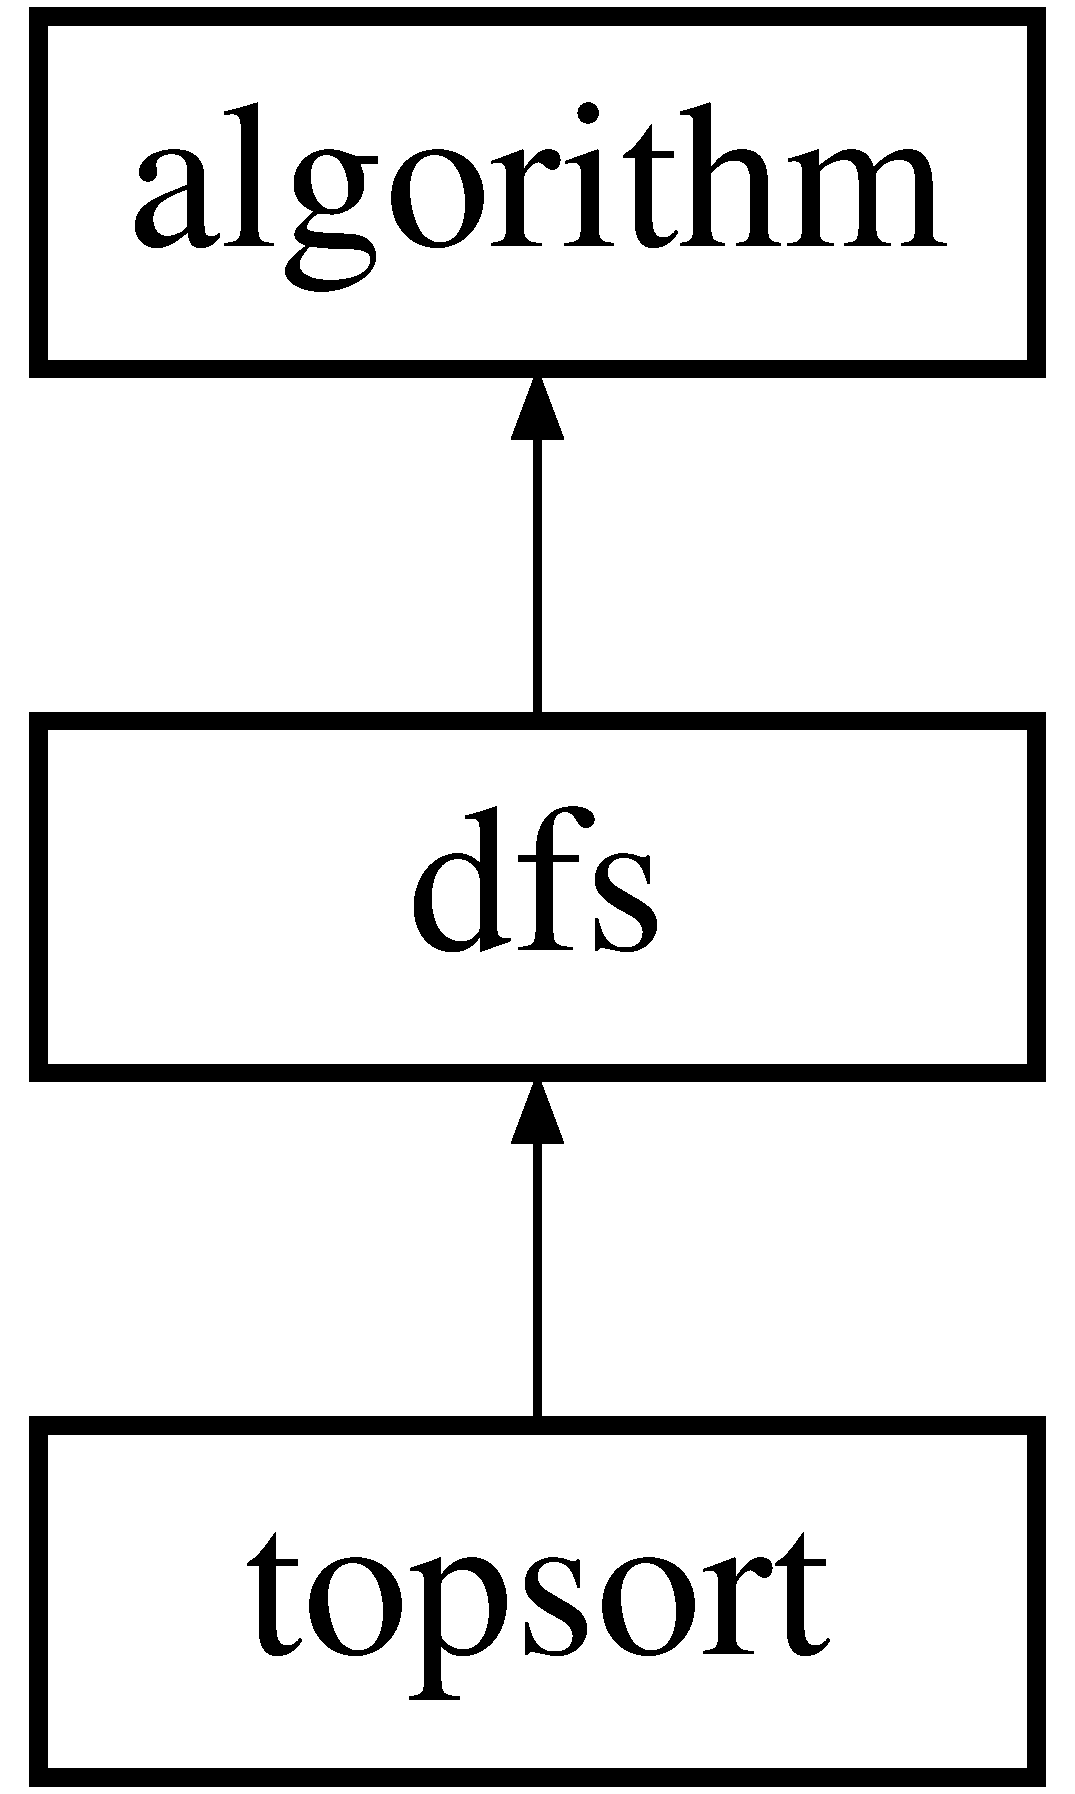
\includegraphics[height=3.000000cm]{classtopsort}
\end{center}
\end{figure}
\subsection*{Public Types}
\begin{DoxyCompactItemize}
\item 
\mbox{\Hypertarget{classtopsort_aaaa250b99c25e7d045b8adf72707fc32}\label{classtopsort_aaaa250b99c25e7d045b8adf72707fc32}} 
typedef list$<$ \mbox{\hyperlink{classnode}{node}} $>$\+::const\+\_\+iterator {\bfseries topsort\+\_\+iterator}
\end{DoxyCompactItemize}
\subsection*{Public Member Functions}
\begin{DoxyCompactItemize}
\item 
\mbox{\hyperlink{classtopsort_a76a9055969b9dbf006320040be9fd5e6}{topsort}} ()
\item 
int \mbox{\hyperlink{classtopsort_a0f0b52c54ffa4d1056ef96f16489f30f}{top\+\_\+num}} (const \mbox{\hyperlink{classnode}{node}} \&n) const
\item 
bool \mbox{\hyperlink{classtopsort_a05a4cb00bbd60859f4939355b23c25f1}{is\+\_\+acyclic}} () const
\item 
topsort\+\_\+iterator \mbox{\hyperlink{classtopsort_ab220dcce845e001b0f737d0dc7751abc}{top\+\_\+order\+\_\+begin}} () const
\item 
topsort\+\_\+iterator \mbox{\hyperlink{classtopsort_ac9b784654ae0c4e9736931d63d03291b}{top\+\_\+order\+\_\+end}} () const
\item 
virtual int \mbox{\hyperlink{classtopsort_a777a9a68c4081d22e7b698ed3c515343}{check}} (\mbox{\hyperlink{classgraph}{graph}} \&G)
\item 
virtual void \mbox{\hyperlink{classtopsort_af93d2f617ceae83ee2a4f9106fbc32c3}{reset}} ()
\item 
virtual void \mbox{\hyperlink{classtopsort_a21aaf28fc280094ed43288e58d8e3ae1}{init\+\_\+handler}} (\mbox{\hyperlink{classgraph}{graph}} \&G)
\begin{DoxyCompactList}\small\item\em Handler called before the start of D\+FS. \end{DoxyCompactList}\item 
virtual void \mbox{\hyperlink{classtopsort_afd27bb676fd3987456bf71d83c05acb8}{leave\+\_\+handler}} (\mbox{\hyperlink{classgraph}{graph}} \&, \mbox{\hyperlink{classnode}{node}} \&, \mbox{\hyperlink{classnode}{node}} \&)
\begin{DoxyCompactList}\small\item\em Handler called after all the adjacent edges of {\itshape n} have been examined. \end{DoxyCompactList}\item 
virtual void \mbox{\hyperlink{classtopsort_ab42587b5a1e776be5106502dfeb6b0b1}{old\+\_\+adj\+\_\+node\+\_\+handler}} (\mbox{\hyperlink{classgraph}{graph}} \&, \mbox{\hyperlink{classedge}{edge}} \&, \mbox{\hyperlink{classnode}{node}} \&)
\begin{DoxyCompactList}\small\item\em Handler called when a already marked node {\itshape n} connected to the actual node by {\itshape e} is found during the search of all adjacent edges of the actual node. \end{DoxyCompactList}\end{DoxyCompactItemize}
\subsection*{Protected Attributes}
\begin{DoxyCompactItemize}
\item 
\mbox{\Hypertarget{classtopsort_ae04dea9ee7f97be6e0e9673afb601f96}\label{classtopsort_ae04dea9ee7f97be6e0e9673afb601f96}} 
int {\bfseries act\+\_\+top\+\_\+num}
\item 
\mbox{\Hypertarget{classtopsort_ae57da1aae22ed92acd0d84c737a1da2b}\label{classtopsort_ae57da1aae22ed92acd0d84c737a1da2b}} 
\mbox{\hyperlink{classnode__map}{node\+\_\+map}}$<$ int $>$ {\bfseries top\+\_\+numbers}
\item 
\mbox{\Hypertarget{classtopsort_aaff79afb24dd71820c936be2b88027ee}\label{classtopsort_aaff79afb24dd71820c936be2b88027ee}} 
list$<$ \mbox{\hyperlink{classnode}{node}} $>$ {\bfseries top\+\_\+order}
\item 
\mbox{\Hypertarget{classtopsort_a01d94e7627a5660836cc0765ec15727a}\label{classtopsort_a01d94e7627a5660836cc0765ec15727a}} 
bool {\bfseries acyclic}
\end{DoxyCompactItemize}


\subsection{Detailed Description}
Topological sorting. 

Assigns to each node {\ttfamily n} a number {\ttfamily top\+\_\+num} such that for every edge {\ttfamily (u,v)} {\ttfamily top\+\_\+num\mbox{[}u\mbox{]}} $<$ {\ttfamily top\+\_\+num\mbox{[}v\mbox{]}}, if possible, i.\+e. iff the directed graph is acyclic. ~\newline
 

Similar to the testing of biconnectivity, which extends D\+FS to calculate low-\/numbers, the topsort-\/algorithm extends D\+FS to calculate the new numbering (and thus to test whether such a numbering is possible).

In order to traverse all the nodes in the order of its top-\/numbers, a new iterator, {\ttfamily topsort\+\_\+iterator} is provided. 

\subsection{Constructor \& Destructor Documentation}
\mbox{\Hypertarget{classtopsort_a76a9055969b9dbf006320040be9fd5e6}\label{classtopsort_a76a9055969b9dbf006320040be9fd5e6}} 
\index{topsort@{topsort}!topsort@{topsort}}
\index{topsort@{topsort}!topsort@{topsort}}
\subsubsection{\texorpdfstring{topsort()}{topsort()}}
{\footnotesize\ttfamily topsort\+::topsort (\begin{DoxyParamCaption}{ }\end{DoxyParamCaption})\hspace{0.3cm}{\ttfamily [inline]}}

default constructor; enables scanning of the whole\+\_\+graph.

\begin{DoxySeeAlso}{See also}
\mbox{\hyperlink{classdfs_a5232bc41ab202b6278a84bd97c803a0d}{dfs\+::dfs}} 
\end{DoxySeeAlso}


\subsection{Member Function Documentation}
\mbox{\Hypertarget{classtopsort_a777a9a68c4081d22e7b698ed3c515343}\label{classtopsort_a777a9a68c4081d22e7b698ed3c515343}} 
\index{topsort@{topsort}!check@{check}}
\index{check@{check}!topsort@{topsort}}
\subsubsection{\texorpdfstring{check()}{check()}}
{\footnotesize\ttfamily int topsort\+::check (\begin{DoxyParamCaption}\item[{\mbox{\hyperlink{classgraph}{graph}} \&}]{G }\end{DoxyParamCaption})\hspace{0.3cm}{\ttfamily [virtual]}}

Preconditions\+: 
\begin{DoxyItemize}
\item {\ttfamily G} is directed. 
\item D\+FS may be applied 
\end{DoxyItemize}


\begin{DoxyParams}{Parameters}
{\em $<$code$>$\+G$<$/code$>$} & graph. \\
\hline
\end{DoxyParams}
\begin{DoxyReturn}{Returns}
{\ttfamily \mbox{\hyperlink{classalgorithm_af1a0078e153aa99c24f9bdf0d97f6710aae4c1cd7fe8d8cf4b143241a6e7c31cf}{algorithm\+::\+K\+G\+L\+\_\+\+OK}}} if topsort may be applied to {\ttfamily G}. 
\end{DoxyReturn}
\begin{DoxySeeAlso}{See also}
\mbox{\hyperlink{classdfs_a1af70060897529e67910f589b047e576}{dfs\+::check}} 
\end{DoxySeeAlso}


Reimplemented from \mbox{\hyperlink{classdfs_a1af70060897529e67910f589b047e576}{dfs}}.

\mbox{\Hypertarget{classtopsort_a21aaf28fc280094ed43288e58d8e3ae1}\label{classtopsort_a21aaf28fc280094ed43288e58d8e3ae1}} 
\index{topsort@{topsort}!init\+\_\+handler@{init\+\_\+handler}}
\index{init\+\_\+handler@{init\+\_\+handler}!topsort@{topsort}}
\subsubsection{\texorpdfstring{init\+\_\+handler()}{init\_handler()}}
{\footnotesize\ttfamily void topsort\+::init\+\_\+handler (\begin{DoxyParamCaption}\item[{\mbox{\hyperlink{classgraph}{graph}} \&}]{G }\end{DoxyParamCaption})\hspace{0.3cm}{\ttfamily [virtual]}}



Handler called before the start of D\+FS. 


\begin{DoxyParams}{Parameters}
{\em G} & graph for which D\+FS was invoked. \\
\hline
\end{DoxyParams}


Reimplemented from \mbox{\hyperlink{classdfs_acc82574cd42ab8256e685374bee5fabb}{dfs}}.

\mbox{\Hypertarget{classtopsort_a05a4cb00bbd60859f4939355b23c25f1}\label{classtopsort_a05a4cb00bbd60859f4939355b23c25f1}} 
\index{topsort@{topsort}!is\+\_\+acyclic@{is\+\_\+acyclic}}
\index{is\+\_\+acyclic@{is\+\_\+acyclic}!topsort@{topsort}}
\subsubsection{\texorpdfstring{is\+\_\+acyclic()}{is\_acyclic()}}
{\footnotesize\ttfamily bool topsort\+::is\+\_\+acyclic (\begin{DoxyParamCaption}{ }\end{DoxyParamCaption}) const\hspace{0.3cm}{\ttfamily [inline]}}

Tests if graph was acyclic.

\begin{DoxyReturn}{Returns}
true iff graph was acyclic. 
\end{DoxyReturn}
\mbox{\Hypertarget{classtopsort_afd27bb676fd3987456bf71d83c05acb8}\label{classtopsort_afd27bb676fd3987456bf71d83c05acb8}} 
\index{topsort@{topsort}!leave\+\_\+handler@{leave\+\_\+handler}}
\index{leave\+\_\+handler@{leave\+\_\+handler}!topsort@{topsort}}
\subsubsection{\texorpdfstring{leave\+\_\+handler()}{leave\_handler()}}
{\footnotesize\ttfamily void topsort\+::leave\+\_\+handler (\begin{DoxyParamCaption}\item[{\mbox{\hyperlink{classgraph}{graph}} \&}]{G,  }\item[{\mbox{\hyperlink{classnode}{node}} \&}]{n,  }\item[{\mbox{\hyperlink{classnode}{node}} \&}]{f }\end{DoxyParamCaption})\hspace{0.3cm}{\ttfamily [virtual]}}



Handler called after all the adjacent edges of {\itshape n} have been examined. 


\begin{DoxyParams}{Parameters}
{\em G} & graph for which D\+FS was invoked. \\
\hline
{\em n} & actual node. \\
\hline
{\em f} & predecessor. \\
\hline
\end{DoxyParams}


Reimplemented from \mbox{\hyperlink{classdfs_a8071fc4e82deff7ceb2790cd4eb42280}{dfs}}.

\mbox{\Hypertarget{classtopsort_ab42587b5a1e776be5106502dfeb6b0b1}\label{classtopsort_ab42587b5a1e776be5106502dfeb6b0b1}} 
\index{topsort@{topsort}!old\+\_\+adj\+\_\+node\+\_\+handler@{old\+\_\+adj\+\_\+node\+\_\+handler}}
\index{old\+\_\+adj\+\_\+node\+\_\+handler@{old\+\_\+adj\+\_\+node\+\_\+handler}!topsort@{topsort}}
\subsubsection{\texorpdfstring{old\+\_\+adj\+\_\+node\+\_\+handler()}{old\_adj\_node\_handler()}}
{\footnotesize\ttfamily void topsort\+::old\+\_\+adj\+\_\+node\+\_\+handler (\begin{DoxyParamCaption}\item[{\mbox{\hyperlink{classgraph}{graph}} \&}]{G,  }\item[{\mbox{\hyperlink{classedge}{edge}} \&}]{e,  }\item[{\mbox{\hyperlink{classnode}{node}} \&}]{n }\end{DoxyParamCaption})\hspace{0.3cm}{\ttfamily [virtual]}}



Handler called when a already marked node {\itshape n} connected to the actual node by {\itshape e} is found during the search of all adjacent edges of the actual node. 


\begin{DoxyParams}{Parameters}
{\em G} & graph for which D\+FS was invoked. \\
\hline
{\em e} & edge connecting the actual node to the old one. \\
\hline
{\em n} & used node. \\
\hline
\end{DoxyParams}


Reimplemented from \mbox{\hyperlink{classdfs_adf1c667188e632761c63f529537c544c}{dfs}}.

\mbox{\Hypertarget{classtopsort_af93d2f617ceae83ee2a4f9106fbc32c3}\label{classtopsort_af93d2f617ceae83ee2a4f9106fbc32c3}} 
\index{topsort@{topsort}!reset@{reset}}
\index{reset@{reset}!topsort@{topsort}}
\subsubsection{\texorpdfstring{reset()}{reset()}}
{\footnotesize\ttfamily \+\_\+\+\_\+\+K\+G\+L\+\_\+\+B\+E\+G\+I\+N\+\_\+\+N\+A\+M\+E\+S\+P\+A\+CE void topsort\+::reset (\begin{DoxyParamCaption}{ }\end{DoxyParamCaption})\hspace{0.3cm}{\ttfamily [virtual]}}

Reset \begin{DoxySeeAlso}{See also}
\mbox{\hyperlink{classdfs_affaffda8be8418d6dbf396c5b1d6b81a}{dfs\+::reset}} 
\end{DoxySeeAlso}


Reimplemented from \mbox{\hyperlink{classdfs_affaffda8be8418d6dbf396c5b1d6b81a}{dfs}}.

\mbox{\Hypertarget{classtopsort_a0f0b52c54ffa4d1056ef96f16489f30f}\label{classtopsort_a0f0b52c54ffa4d1056ef96f16489f30f}} 
\index{topsort@{topsort}!top\+\_\+num@{top\+\_\+num}}
\index{top\+\_\+num@{top\+\_\+num}!topsort@{topsort}}
\subsubsection{\texorpdfstring{top\+\_\+num()}{top\_num()}}
{\footnotesize\ttfamily int topsort\+::top\+\_\+num (\begin{DoxyParamCaption}\item[{const \mbox{\hyperlink{classnode}{node}} \&}]{n }\end{DoxyParamCaption}) const\hspace{0.3cm}{\ttfamily [inline]}}

Number in topological order.


\begin{DoxyParams}{Parameters}
{\em $<$code$>$n$<$/code$>$} & node. \\
\hline
\end{DoxyParams}
\begin{DoxyReturn}{Returns}
number in topological order. 
\end{DoxyReturn}
\mbox{\Hypertarget{classtopsort_ab220dcce845e001b0f737d0dc7751abc}\label{classtopsort_ab220dcce845e001b0f737d0dc7751abc}} 
\index{topsort@{topsort}!top\+\_\+order\+\_\+begin@{top\+\_\+order\+\_\+begin}}
\index{top\+\_\+order\+\_\+begin@{top\+\_\+order\+\_\+begin}!topsort@{topsort}}
\subsubsection{\texorpdfstring{top\+\_\+order\+\_\+begin()}{top\_order\_begin()}}
{\footnotesize\ttfamily topsort\+\_\+iterator topsort\+::top\+\_\+order\+\_\+begin (\begin{DoxyParamCaption}{ }\end{DoxyParamCaption}) const\hspace{0.3cm}{\ttfamily [inline]}}

Iterate through nodes in topsort-\/order.

\begin{DoxyReturn}{Returns}
start-\/iterator. 
\end{DoxyReturn}
\mbox{\Hypertarget{classtopsort_ac9b784654ae0c4e9736931d63d03291b}\label{classtopsort_ac9b784654ae0c4e9736931d63d03291b}} 
\index{topsort@{topsort}!top\+\_\+order\+\_\+end@{top\+\_\+order\+\_\+end}}
\index{top\+\_\+order\+\_\+end@{top\+\_\+order\+\_\+end}!topsort@{topsort}}
\subsubsection{\texorpdfstring{top\+\_\+order\+\_\+end()}{top\_order\_end()}}
{\footnotesize\ttfamily topsort\+\_\+iterator topsort\+::top\+\_\+order\+\_\+end (\begin{DoxyParamCaption}{ }\end{DoxyParamCaption}) const\hspace{0.3cm}{\ttfamily [inline]}}

Iterate through nodes in topsort-\/order.

\begin{DoxyReturn}{Returns}
end-\/iterator. 
\end{DoxyReturn}


The documentation for this class was generated from the following files\+:\begin{DoxyCompactItemize}
\item 
include/\+K\+G\+L/topsort.\+h\item 
src/topsort.\+cpp\end{DoxyCompactItemize}

%--- End generated contents ---

% Index
\backmatter
\newpage
\phantomsection
\clearemptydoublepage
\addcontentsline{toc}{chapter}{Index}
\printindex

\end{document}
